\documentclass[twoside]{tufte-book}

%\hypersetup{colorlinks}% uncomment this line if you prefer colored hyperlinks (e.g., for onscreen viewing)

%%
% Book metadata
\title{Vision-Based 
       Estimation and 
       Control of 
       Multirotor and 
       Winged-VTOL Systems}
\author{Randal W. Beard}
\publisher{Brigham Young University}

%%%%%%%%%%%%%%%%%%%%%%%%%%%%%%%%%%%%%%%%%%%%%%%%%%%%%%%%%
%                tufte-book style
%%%%%%%%%%%%%%%%%%%%%%%%%%%%%%%%%%%%%%%%%%%%%%%%%%%%%%%%%

%%
% If they're installed, use Bergamo and Chantilly from www.fontsite.com.
% They're clones of Bembo and Gill Sans, respectively.
%\IfFileExists{bergamo.sty}{\usepackage[osf]{bergamo}}{}% Bembo
%\IfFileExists{chantill.sty}{\usepackage{chantill}}{}% Gill Sans

%\usepackage{microtype}

%%
% Just some sample text
\usepackage{lipsum}

%%
% For nicely typeset tabular material
\usepackage{booktabs}

%%
% For graphics / images
\usepackage[pdftex]{graphicx}
\setkeys{Gin}{width=\linewidth,totalheight=\textheight,keepaspectratio}
  \graphicspath{{./figures/}}
  \DeclareGraphicsExtensions{.pdf,.jpg,.png}

% The fancyvrb package lets us customize the formatting of verbatim
% environments.  We use a slightly smaller font.
\usepackage{fancyvrb}
\fvset{fontsize=\normalsize}

%%
% Prints argument within hanging parentheses (i.e., parentheses that take
% up no horizontal space).  Useful in tabular environments.
\newcommand{\hangp}[1]{\makebox[0pt][r]{(}#1\makebox[0pt][l]{)}}

%%
% Prints an asterisk that takes up no horizontal space.
% Useful in tabular environments.
\newcommand{\hangstar}{\makebox[0pt][l]{*}}

%%
% Prints a trailing space in a smart way.
\usepackage{xspace}

%%
% Some shortcuts for Tufte's book titles.  The lowercase commands will
% produce the initials of the book title in italics.  The all-caps commands
% will print out the full title of the book in italics.
\newcommand{\vdqi}{\textit{VDQI}\xspace}
\newcommand{\ei}{\textit{EI}\xspace}
\newcommand{\ve}{\textit{VE}\xspace}
\newcommand{\be}{\textit{BE}\xspace}
\newcommand{\VDQI}{\textit{The Visual Display of Quantitative Information}\xspace}
\newcommand{\EI}{\textit{Envisioning Information}\xspace}
\newcommand{\VE}{\textit{Visual Explanations}\xspace}
\newcommand{\BE}{\textit{Beautiful Evidence}\xspace}

\newcommand{\TL}{Tufte-\LaTeX\xspace}

% Prints the month name (e.g., January) and the year (e.g., 2008)
\newcommand{\monthyear}{%
  \ifcase\month\or January\or February\or March\or April\or May\or June\or
  July\or August\or September\or October\or November\or
  December\fi\space\number\year
}


% Prints an epigraph and speaker in sans serif, all-caps type.
\newcommand{\openepigraph}[2]{%
  %\sffamily\fontsize{14}{16}\selectfont
  \begin{fullwidth}
  \sffamily\large
  \begin{doublespace}
  \noindent\allcaps{#1}\\% epigraph
  \noindent\allcaps{#2}% author
  \end{doublespace}
  \end{fullwidth}
}

% Inserts a blank page
\newcommand{\blankpage}{\newpage\hbox{}\thispagestyle{empty}\newpage}

\usepackage{units}

% Typesets the font size, leading, and measure in the form of 10/12x26 pc.
\newcommand{\measure}[3]{#1/#2$\times$\unit[#3]{pc}}

% Macros for typesetting the documentation
\newcommand{\hlred}[1]{\textcolor{Maroon}{#1}}% prints in red
\newcommand{\hangleft}[1]{\makebox[0pt][r]{#1}}
\newcommand{\hairsp}{\hspace{1pt}}% hair space
\newcommand{\hquad}{\hskip0.5em\relax}% half quad space
\newcommand{\TODO}{\textcolor{red}{\bf TODO!}\xspace}
\newcommand{\na}{\quad--}% used in tables for N/A cells
\providecommand{\XeLaTeX}{X\lower.5ex\hbox{\kern-0.15em\reflectbox{E}}\kern-0.1em\LaTeX}
\newcommand{\tXeLaTeX}{\XeLaTeX\index{XeLaTeX@\protect\XeLaTeX}}
% \index{\texttt{\textbackslash xyz}@\hangleft{\texttt{\textbackslash}}\texttt{xyz}}
\newcommand{\tuftebs}{\symbol{'134}}% a backslash in tt type in OT1/T1
\newcommand{\doccmdnoindex}[2][]{\texttt{\tuftebs#2}}% command name -- adds backslash automatically (and doesn't add cmd to the index)
\newcommand{\doccmddef}[2][]{%
  \hlred{\texttt{\tuftebs#2}}\label{cmd:#2}%
  \ifthenelse{\isempty{#1}}%
    {% add the command to the index
      \index{#2 command@\protect\hangleft{\texttt{\tuftebs}}\texttt{#2}}% command name
    }%
    {% add the command and package to the index
      \index{#2 command@\protect\hangleft{\texttt{\tuftebs}}\texttt{#2} (\texttt{#1} package)}% command name
      \index{#1 package@\texttt{#1} package}\index{packages!#1@\texttt{#1}}% package name
    }%
}% command name -- adds backslash automatically
\newcommand{\doccmd}[2][]{%
  \texttt{\tuftebs#2}%
  \ifthenelse{\isempty{#1}}%
    {% add the command to the index
      \index{#2 command@\protect\hangleft{\texttt{\tuftebs}}\texttt{#2}}% command name
    }%
    {% add the command and package to the index
      \index{#2 command@\protect\hangleft{\texttt{\tuftebs}}\texttt{#2} (\texttt{#1} package)}% command name
      \index{#1 package@\texttt{#1} package}\index{packages!#1@\texttt{#1}}% package name
    }%
}% command name -- adds backslash automatically
\newcommand{\docopt}[1]{\ensuremath{\langle}\textrm{\textit{#1}}\ensuremath{\rangle}}% optional command argument
\newcommand{\docarg}[1]{\textrm{\textit{#1}}}% (required) command argument
\newenvironment{docspec}{\begin{quotation}\ttfamily\parskip0pt\parindent0pt\ignorespaces}{\end{quotation}}% command specification environment
\newcommand{\docenv}[1]{\texttt{#1}\index{#1 environment@\texttt{#1} environment}\index{environments!#1@\texttt{#1}}}% environment name
\newcommand{\docenvdef}[1]{\hlred{\texttt{#1}}\label{env:#1}\index{#1 environment@\texttt{#1} environment}\index{environments!#1@\texttt{#1}}}% environment name
\newcommand{\docpkg}[1]{\texttt{#1}\index{#1 package@\texttt{#1} package}\index{packages!#1@\texttt{#1}}}% package name
\newcommand{\doccls}[1]{\texttt{#1}}% document class name
\newcommand{\docclsopt}[1]{\texttt{#1}\index{#1 class option@\texttt{#1} class option}\index{class options!#1@\texttt{#1}}}% document class option name
\newcommand{\docclsoptdef}[1]{\hlred{\texttt{#1}}\label{clsopt:#1}\index{#1 class option@\texttt{#1} class option}\index{class options!#1@\texttt{#1}}}% document class option name defined
\newcommand{\docmsg}[2]{\bigskip\begin{fullwidth}\noindent\ttfamily#1\end{fullwidth}\medskip\par\noindent#2}
\newcommand{\docfilehook}[2]{\texttt{#1}\index{file hooks!#2}\index{#1@\texttt{#1}}}
\newcommand{\doccounter}[1]{\texttt{#1}\index{#1 counter@\texttt{#1} counter}}



%%%%%%%%%%%%%%%%%%%%%%%%%%%%%%%%%%%%%%%%%%%%%%%%%%%%%%%%%
%                Packages
%%%%%%%%%%%%%%%%%%%%%%%%%%%%%%%%%%%%%%%%%%%%%%%%%%%%%%%%%
\usepackage{amsmath,amssymb,amstext,amsfonts}

\usepackage[T1]{fontenc}
\usepackage[latin9]{inputenc}
\usepackage{lmodern}
\usepackage{latexsym}
%\usepackage[pdftex]{graphicx}
%  \graphicspath{{./figures/}}
%  \DeclareGraphicsExtensions{.pdf,.jpg,.png}
\usepackage{color}
\usepackage{subfigmat}
%\usepackage{keyval,times}
\usepackage{fancyhdr}
	\pagestyle{fancy}
	\fancyhead[LE,RO]{} % make is so nothing appears in header on left for even and right for odd pages
\usepackage{theorem}
\usepackage{nicefrac}
\usepackage{listings}  % for code
\usepackage[small,bf]{caption}  % for better figure captions
\usepackage{makeidx}  % for making an index
\usepackage{longtable}
\usepackage{units}
\usepackage{algorithmic,algorithm}
\usepackage{hyperref}
\hypersetup{%
   pdftitle={quadrotorbook},
   pdfauthor={R. Beard, T. McLain},
   pdfkeywords={Multi-rotors, attitude estimation, control.},
   bookmarksnumbered,
   pdfstartview={FitH},
   colorlinks=true,
   breaklinks=true,
   citecolor=blue,
   linkcolor=blue,
}%
\usepackage{pdfpages}
%\usepackage{tocloft}  % change spacing in table of contents
%	\setlength\cftparskip{-2pt}
%	\setlength\cftbeforechapskip{0pt}
\usepackage{cancel} % cancel marks
\usepackage{fancybox}  % oval boxes in tables

% Generates the index
\usepackage{makeidx}
\makeindex

\setcounter{secnumdepth}{3}  % defines which sections are numbered


%%%%%%%%%%%%%%%%%%%%%%%%%%%%%%%%%%%%%%%%%%%%%%%%%%%%%%%%%
%                Macros
%%%%%%%%%%%%%%%%%%%%%%%%%%%%%%%%%%%%%%%%%%%%%%%%%%%%%%%%%
\newcommand{\OMIT}[1]{{}}
%\newcommand{\TODO}[1]{{\color{green} To do: #1}}
\newcommand{\rwbcomment}[1]{{\color{red} RWB: #1}}
\newcommand{\twmcomment}[1]{{\color{blue} TWM: #1}}
\newcommand{\jbwcomment}[1]{{\color{red} JBW: #1}}
\newcommand{\pde}[2]{\frac{\partial#1}{\partial#2}}
\newcommand{\trace}[1]{\text{tr}\left(#1\right)}
\newcommand{\rank}[1]{\text{rank}\left(#1\right)}
\renewcommand{\ss}[1]{\left\lfloor#1\right\rfloor_{\times}}
%\renewcommand{\ss}[1]{{#1^\wedge}}
\newcommand{\cov}{\text{\em cov}}
\newcommand{\var}{\text{\em var}}
\newcommand{\stdev}{\text{\em stdev}}
\newcommand{\defeq}{\stackrel{\triangle}{=}}
\newcommand{\norm}[1]{\left\|#1\right\|}
\newcommand{\abs}[1]{\left|#1\right|}
\newcommand{\re}{{\mathbb{R}}}
\newcommand{\tr}{\top}
\newcommand{\half}{\frac{1}{2}}
%\newcommand{\Vair}{V_{\text{air}}}
%\newcommand{\Vgrd}{V_{\text{grd}}}
\newcommand{\mass}{\mathsf{m}}
\newcommand{\Acal}{{\mathcal{A}}}
\newcommand{\Ccal}{{\mathcal{C}}}
\newcommand{\Gcal}{{\mathcal{G}}}
\newcommand{\Hcal}{{\mathcal{H}}}
\newcommand{\Jcal}{{\mathcal{J}}}
\newcommand{\Lcal}{{\mathcal{L}}}
\newcommand{\Rcal}{{\mathcal{R}}}
\newcommand{\Scal}{{\mathcal{S}}}
\newcommand{\Ucal}{{\mathcal{U}}}
\newcommand{\Xcal}{\mathcal{X}}
\newcommand{\abf}{\mathbf{a}}
\newcommand{\bbf}{\mathbf{b}}
\newcommand{\cbf}{\mathbf{c}}
\newcommand{\dbf}{\mathbf{d}}
\newcommand{\ebf}{\mathbf{e}}
\newcommand{\fbf}{\mathbf{f}}
\newcommand{\gbf}{\mathbf{g}}
\newcommand{\hbf}{\mathbf{h}}
\newcommand{\ibf}{\mathbf{i}}
\newcommand{\jbf}{\mathbf{j}}
\newcommand{\kbf}{\mathbf{k}}
\newcommand{\lbf}{\boldsymbol{\ell}}
\newcommand{\mbf}{\mathbf{m}}
\newcommand{\nbf}{\mathbf{n}}
\newcommand{\pbf}{\mathbf{p}}
\newcommand{\qbf}{\mathbf{q}}
\newcommand{\rbf}{\mathbf{r}}
\newcommand{\sbf}{\mathbf{s}}
\newcommand{\tbf}{\mathbf{t}}
\newcommand{\ubf}{\mathbf{u}}
\newcommand{\vbf}{\mathbf{v}}
\newcommand{\wbf}{\mathbf{w}}
\newcommand{\xbf}{\mathbf{x}}
\newcommand{\ybf}{\mathbf{y}}
\newcommand{\zbf}{\mathbf{z}}
\newcommand{\Fbf}{\mathbf{F}}
\newcommand{\Ibf}{\mathbf{I}}
\newcommand{\Jbf}{\mathbf{J}}
\newcommand{\Mbf}{\mathbf{M}}
\newcommand{\Tbf}{\mathbf{T}}
\newcommand{\Vbf}{\mathbf{V}}
\newcommand{\sth}{\text{s}_\theta}
\newcommand{\cth}{\text{c}_\theta}
\newcommand{\sph}{\text{s}_\phi}
\newcommand{\cph}{\text{c}_\phi}
\newcommand{\sps}{\text{s}_\psi}
\newcommand{\cps}{\text{c}_\psi}
\newcommand{\deltabf}{\boldsymbol{\delta}}
\newcommand{\omegabf}{\boldsymbol{\omega}}
\newcommand{\Omegabf}{\boldsymbol{\Omega}}
\newcommand{\Taubf}{\mathbf{\mathcal{T}}}
\newcommand{\zetabf}{\boldsymbol{\zeta}}
\newcommand{\zerobf}{\mathbf{0}}
\newcommand{\taubf}{\boldsymbol{\tau}}
\newcommand{\nubf}{\boldsymbol{\nu}}
\newcommand{\mubf}{\boldsymbol{\mu}}
\newcommand{\epsilonbf}{\boldsymbol{\epsilon}}
\newcommand{\ellbf}{\boldsymbol{\ell}}
\newcommand{\degrees}[1]{{#1}^\circ}
\newcommand{\cross}{\times}
\newcommand{\oneyear}{\rule{10mm}{3mm}}
\newcommand{\twoyears}{\multicolumn{2}{|c|}{\rule{26mm}{3mm}}}
\newcommand{\threeyears}{\multicolumn{3}{|c|}{\rule{44mm}{3mm}}}
\newcommand{\ith}{$i^{\text{th}}~$}
\newtheorem{theorem}{Theorem}[section]
\newtheorem{corollary}[theorem]{Corollary}
\newtheorem{definition}[theorem]{Definition}
\newtheorem{lemma}[theorem]{Lemma}
\newtheorem{property}[theorem]{Property}
\def\proof{\hspace{1em}{\it Proof: }}
\def\endproof{\hspace*{\fill}~$\blacksquare$\par\endtrivlist\unskip}
\newcommand{\subsubsubsection}[1]{{\par\noindent\it #1:}}
\def\proof{\hspace{1em}{\it Proof: }}
\def\endproof{\hspace*{\fill}~$\blacksquare$\par\endtrivlist\unskip}
\DeclareMathOperator{\sign}{sign}
\DeclareMathOperator{\sinc}{sinc}
\DeclareMathOperator{\atan2}{atan2}
\DeclareMathOperator{\asin}{asin}
\hyphenation{pseudo-range}

% define greybox:  for text in a grey box use \greybox{stuff}.
\long\def\greybox#1{%
    \newbox\contentbox%
    \newbox\bkgdbox%
    \setbox\contentbox\hbox to \hsize{%
        \vtop{
            \kern\columnsep
            \hbox to \hsize{%
                \kern\columnsep%
                \advance\hsize by -2\columnsep%
                \setlength{\textwidth}{\hsize}%
                \vbox{
                    \parskip=\baselineskip
                    \parindent=0bp
                    #1
                }%
                \kern\columnsep%
            }%
            \kern\columnsep%
        }%
    }%
    \setbox\bkgdbox\vbox{
        \pdfliteral{0.85 0.85 0.85 rg}
        \hrule width  \wd\contentbox %
               height \ht\contentbox %
               depth  \dp\contentbox
        \pdfliteral{0 0 0 rg}
    }%
    \wd\bkgdbox=0bp%
    \vbox{\hbox to \hsize{\box\bkgdbox\box\contentbox}}%
    \vskip\baselineskip%
}
% end definition of greybox

%%%%%%%%%%%%%%%%%%%%%%%%%%%%%%%%%%%%%%%%%%%%%%%%%%%%%%%%%
%                End Macros
%%%%%%%%%%%%%%%%%%%%%%%%%%%%%%%%%%%%%%%%%%%%%%%%%%%%%%%%%

%%%%%%%%%%%%%%%%%%%%%%%%%%%%%%%%%%%%%%%%%%%%%%%%%%%%%%%%%
%                James Jackson Macros
%%%%%%%%%%%%%%%%%%%%%%%%%%%%%%%%%%%%%%%%%%%%%%%%%%%%%%%%%

%\global\long\def\v{\mathbf{v}}%
%
%\global\long\def\u{\mathbf{u}}%
%
%\global\long\def\a{\mathbf{a}}%
%
%\global\long\def\b{\mathbf{b}}%
%
%\global\long\def\c{\mathbf{c}}%
%
%\global\long\def\w{\boldsymbol{\omega}}%
%
%\global\long\def\p{\mathbf{p}}%
%
%\global\long\def\t{\mathbf{t}}%
%
%\global\long\def\i{\mathbf{i}}%
%
%\global\long\def\j{\mathbf{j}}%
%
%\global\long\def\e{\mathbf{e}}%
%
%\global\long\def\k{\mathbf{k}}%
%
%\global\long\def\r{\mathbf{r}}%
%
%\global\long\def\d{\mathbf{d}}%
%
%\global\long\def\x{\mathbf{x}}%
%
%\global\long\def\y{\mathbf{y}}%
%
%\global\long\def\q{\mathbf{q}}%
%
%\global\long\def\qq{\Gamma}%
%
%\global\long\def\qr{\q_{r}}%
%
%\global\long\def\qd{\q_{d}}%
%
%\global\long\def\SO{\mathit{SO}}%
%
%\global\long\def\SE{\mathit{SE}}%
%
%\global\long\def\skew#1{\left\lfloor #1\right\rfloor _{\times}}%
%
%\global\long\def\norm#1{\left\Vert #1\right\Vert }%
%
%\global\long\def\grey#1{\textcolor{gray}{#1}}%
%
%\global\long\def\abs#1{\left|#1\right|}%
%
%\global\long\def\S{\mathcal{S}}%
%
%\global\long\def\dd{\boldsymbol{\delta}}%
%
%\global\long\def\Ad{\textrm{Ad}}%
\newcommand{\Ad}{\textnormal{Ad}}
%
%\global\long\def\SU{\mathit{SU}}%
%
%\global\long\def\R{\mathbb{R}}%
%
%\global\long\def\so{\mathfrak{so}}%
%
%\global\long\def\se{\mathfrak{se}}%
%
%\global\long\def\su{\mathfrak{su}}%
\newcommand{\so}{\mathfrak{so}}
\newcommand{\su}{\mathfrak{su}}
\newcommand{\se}{\mathfrak{se}}

%%%%%%%%%%%%%%%%%%%%%%%%%%%%%%%%%%%%%%%%%%%%%%%%%%%%%%%%%
%                End James Jackson Macros
%%%%%%%%%%%%%%%%%%%%%%%%%%%%%%%%%%%%%%%%%%%%%%%%%%%%%%%%%


%%%%%%%%%%%%%%%%%%%%%%%%%%%%%%%%%%%%%%%%%%%%%%%%%%%%%%%%%
%                Begin Formatting
%%%%%%%%%%%%%%%%%%%%%%%%%%%%%%%%%%%%%%%%%%%%%%%%%%%%%%%%%

%%% Commented these lines out for PUP
%\oddsidemargin 0.0in \evensidemargin 0.0in \marginparwidth 0pt
%\marginparsep 0pt \topmargin 0pt \headsep 0.25in \footskip 0.4in
%\textheight 8.5in \textwidth 6.5in \hoffset 0pt \voffset 0pt
%\paperheight 11in \paperwidth 8.5in \headheight 14pt
%\renewcommand{\baselinestretch}{1.2}

%\pagestyle{fancy}
%\renewcommand{\headrulewidth}{0pt}
%\renewcommand{\headsep}{30pt}
%\renewcommand{\chaptermark}[1]{\markboth{#1}{}}
%%\renewcommand{\sectionmark}[1]{\markright{\thesection\ #1}}
%\lhead[\fancyplain{}{\textsf{\bfseries\small\thepage}}]{\fancyplain{}{\textsf{\small\leftmark}}}
%%\rhead[\fancyplain{}{\bfseries\small\rightmark}]{\fancyplain{}{\bfseries\small\thepage}}
%\rhead[\fancyplain{}{\textsf{\small{Chapter}}~\textsf{\small\thechapter}}]{\fancyplain{}{\textsf{\bfseries\small\thepage}}}
%\cfoot{}
%
%\makeatletter
%\newenvironment{hw}{%
%  \renewcommand{\labelenumi}{\thechapter.\theenumi}%
%  \renewcommand{\p@enumi}{\thechapter.}%
%     \begin{enumerate}}{\end{enumerate}}
%\makeatother

%%%%%%%%%%%%%%%%%%%%%%%%%%%%%%%%%%%%%%%%%%%%%%%%%%%%%%%%%
%                End Formatting
%%%%%%%%%%%%%%%%%%%%%%%%%%%%%%%%%%%%%%%%%%%%%%%%%%%%%%%%%


%\includeonly{chap2_preliminaries/preliminaries}
%\includeonly{chap4_trajectory_following/trajectory_following}
%\includeonly{chap5_trajectory_planning/trajectory_planning}
%\includeonly{chap6_camera_features/camera_features}
%\includeonly{chap7_optical_flow/optical_flow}
%\includeonly{chap8_scene_reconstruction/scene_reconstruction}
%\includeonly{chap9_visual_servoing/visual_servoing}
%\includeonly{chap10_tracking/tracking}
\begin{document}

% Front matter
\frontmatter


\maketitle


% v.4 copyright page
\newpage
\begin{fullwidth}
~\vfill
\thispagestyle{empty}
\setlength{\parindent}{0pt}
\setlength{\parskip}{\baselineskip}
Copyright \copyright\ 2020 Randal W. Beard

\par\smallcaps{Published by \thanklesspublisher}

\par\smallcaps{Typeset using tufte-latex.github.io/tufte-latex/}

\par\textit{Current version: \monthyear}
\end{fullwidth}

%\tableofcontents
%\listoffigures
%\listoftables
%\hypertarget{contents}{}

\cleardoublepage
~\vfill
\begin{doublespace}
\noindent\fontsize{18}{22}\selectfont\itshape
\nohyphenation
Dedicated to ...
\end{doublespace}
\vfill
\vfill

\cleardoublepage

%%%%%%%%%%%%%%%%%%%%%%%%%%%%%%%%%%%%%%%%%%%%%%%%%%%%%%%%%%%%%%%%%%%%
\mainmatter

\setcounter{tocdepth}{2}
\tableofcontents
%\hypertarget{contents}{}
{\Huge 
\par\noindent{\em Contents}
}

\vspace{1cm}

{\Large
\par\indent {\em Chapter 1.} \nameref{chap:introduction}
}

\vspace{1cm}

{\huge
\par\noindent{\em Part I.  Models \& Control}
}

{\Large
\par\indent {\em Chapter 2.} \nameref{chap:preliminaries}
\par\indent {\em Chapter 3.} \nameref{chap:multirotor}
\par\indent {\em Chapter 4.} \nameref{chap:trajectory_following}
\par\indent {\em Chapter 5.} \nameref{chap:trajectory_planning}
}
                 
\vspace{1cm}

{\huge
\par\noindent{\em Part II.  Vision Based Flight}
}
{\Large
\par\indent {\em Chapter 6.} \nameref{chap:camera_features}
\par\indent {\em Chapter 7.} \nameref{chap:optical_flow}
\par\indent {\em Chapter 8.} \nameref{chap:scene_reconstruction}
\par\indent {\em Chapter 9.} \nameref{chap:visual_servoing}
\par\indent {\em Chapter 10.} \nameref{chap:tracking}
}

\vspace{1cm}

{\huge
\par\noindent{\em Part III.  Vision Based Estimation}
}
{\Large
\par\indent {\em Chapter 11.} \nameref{chap:attitude_estimation}
\par\indent {\em Chapter 12.} \nameref{chap:trajectory_estimation}
\par\indent {\em Chapter 13.} \nameref{chap:visual_odometry}
\par\indent {\em Chapter 14.} \nameref{chap:visual_SLAM}
}

\vspace{1cm}

{\huge
\par\noindent{\em Appendices}
}
{\Large
%\par\indent {\em Appendix A.} \nameref{app:holodeck}
%\par\indent {\em Appendix B.} \nameref{app:rosflight}
}




\fancypagestyle{plain}{% for chapter starting pages
  %\fancyhf{}% clears header fields
  \rfoot{\hyperlink{contents}{TOC}}
  }
\rfoot{\hyperlink{contents}{TOC}}

\chapter*{Contributors}

The following individuals have contributed section to this book.  Their assistance and insight have been invaluable, and their contributions are gratefully acknowledged.


\begin{tabular}{l|r}
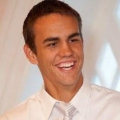
\includegraphics[width=.25\linewidth]{contributors/james_jackson} & 
\begin{minipage}{0.75\linewidth}
	James Jackson was a PhD student at BYU from 2014--2018.  He is currently at Aurora Innovation.
\end{minipage} \\
%
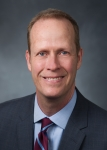
\includegraphics[width=.25\linewidth]{contributors/tim_mclain} & 
\begin{minipage}{0.75\linewidth}
		Tim McLain is a professor in the Department of Mechanical Engineering at Brigham Young University.
\end{minipage} \\
%
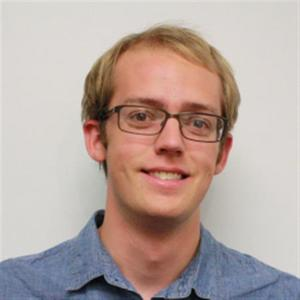
\includegraphics[width=.25\linewidth]{contributors/jacob_willis} & 
\begin{minipage}{0.75\linewidth}
	Jacob Willis is currently a graduate student in the Electrical and Computer Engineering Department at Brigham Young University.
\end{minipage} \\	
%
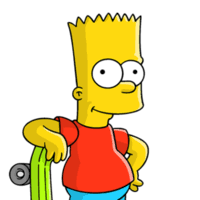
\includegraphics[width=.25\linewidth]{contributors/jake_johnson} & 
\begin{minipage}{0.75\linewidth}
	Jake Johnson is currently a graduate student in the Electrical and Computer Engineering Department at Brigham Young University.
\end{minipage} \\	
	

\end{tabular}

%!TEX root =../quadrotorbook.tex
\chapter{Introduction}
\label{chap:introduction}


The book will be organized around the architecture shown in Figure~\ref{fig:intro_architecture}.

\begin{figure*}[h]
   \centering
   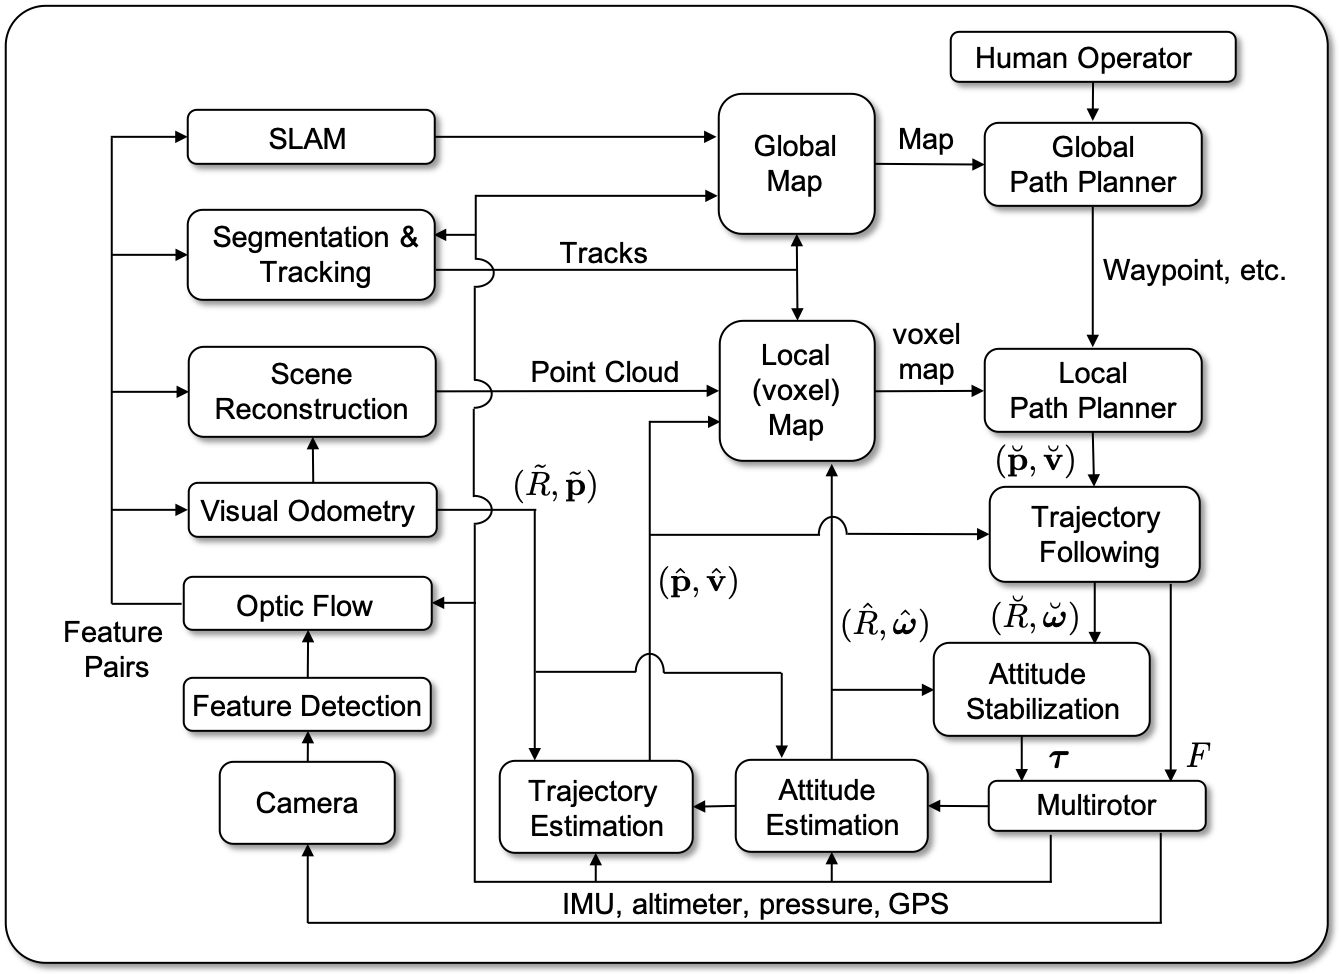
\includegraphics[width=\linewidth]{chap1_intro/figures/architecture} 
   \caption{Software architecture for multirotor estimation and control.}
   \label{fig:intro_architecture}
\end{figure*}

In the bottom right corner is the {\em Multirotor} block representing both the physical flying vehicle and the onboard sensors, including IMU, altimeter, pressure sensors, and possibly a GNSS receiver.  We also assume that the platform has a camera, which we have drawn in its own block.  The equations of motion for the multirotor and the mathematical models for the sensors will be described in Chapter~\ref{chap:multirotor}.  The commanded inputs to the multirotor will be assumed to be the force in the body $z$-axis $F$, and the torque applied to the body $\taubf$.  
%
The {\em Attitude Stabilization} block is discussed in Chapter~\ref{chap:attitude_control}.  In the literature, three different representations for attitude are commonly used, namely Euler angles, quaternions, and rotation matrices.  We will describe attitude stabilization schemes for each representation.  The output of the attitude stabilization block is the applied torque $\taubf$.  The input is the desired attitude $\breve{R}$ and the desired angular rate $\breve{\omegabf}$
%
The {\em Trajectory Following} block is discussed in Chapter~\ref{chap:trajectory_following}.  The input to the trajectory follower is the desired position $\breve{\pbf}$ and the desired velocity $\breve{\vbf}$.  

The second part of the book is concerned with cameras, computer vision, and state estimation.  The {\em Camera} and {\em Feature Detection} blocks shown in Figure~\ref{fig:intro_architecture} are described in Chaper~\ref{chap:camera_features}.  {\em Optical Flow} is discussed in Chapter~\ref{chap:optical_flow}, both how optic flow is computed, as well as how it can be used to navigate a multirotor through urban canyons.  
%
{\em Visual Odometry} is discussed in Chapter~\ref{chap:visual_odometry}.  We then return to the important task of state estimation.  {\em Attitude Estimation} is described in Chapter~\ref{chap:attitude_estimation}, where we include estimation schemes that use feature matching, optic flow, and visual odometry.  In a similar way, {\em Trajectory Estimation} is described in Chapter~\ref{chap:trajectory_estimation}. 

The final part of the book focuses on mapping and planning.  {\em Scene Reconstruction} using a {\em Local Voxel Map} is detailed in Chapter~\ref{chap:scene_reconstruction}.  {\em Segmentation and Tracking} is discussed in Chapter~\ref{chap:tracking}.  The {\em Local Path Planner} is then described in Chapter~\ref{chap:local_planner} where we describe differential flatness, spline-based planning, and visual servoing.  One particular implementation of Simultaneous Localization and Mapping ({\em SLAM}) is then described in Chapter~\ref{chap:SLAM}, and global path planning using the global map created by SLAM is described in Chapter~\ref{chap:global_planner}.







% part I
\part{Models \& Control \& Planning}
%!TEX root =../quadrotorbook.tex
\chapter{Preliminaries}
\label{chap:preliminaries}

Author: RWB, James Jackson

This chapter motivates and derives many commonly-used formulae used
when performing coordinate transformations in robotics and computer
vision. There are a many great resources on this topic
\cite[-2in]{Barfoot2019}\cite[-1in]{Drummond2014}\cite[1in]{Ethan2019}\cite[2in]{Sola2019}.

%
%and I do not pretend to be adding anything particularly novel to the
%field of knowledge in this area. However, this has personally been
%a source of great confusion to me over the years and I wanted to derive
%these concepts from basics, highlighting the gotchas that I have encountered
%along the way. I hope that this ends up being useful to people new
%to the field of robotics or computer vision. 

%As many of my fellow graduate students and I used to say, ``The two
%hardest problems in robotics are coordinate frames and naming things.''
%While this won't help you much with the second problem, this will
%hopefully help dispel a lot of the confusion I encountered at first.

One difference with this document when compared with others is the
use of extra notation throughout. This notation is much more verbose
than a lot of other literature on robotics or computer vision, but
the extra syntax clarifies what is going on, and makes it easier 
%for
%someone like me (who likes to think of these ideas in terms of physical
%relationships, rather than abstract mathematical ideas) 
to visualize
and understand what is going on. 
%The extra notation has also allowed
%me to make distinctions between different fields of research that
%may have different conventions when it comes to transformations.


%-------------------------------------------------------------
\section{Notation}

Throughout the book we will use lower case symbols to represent scalars, bold lower case to represent vectors, and upper case to represent matrices. Hence
\begin{align*}
A &= \begin{pmatrix} \abf_1 & \abf_2 & \dots & \abf_n\end{pmatrix} \\
  &= \begin{pmatrix} a_{11} & a_{12} & \dots & a_{1n} \\
                     a_{21} & a_{22} & \dots & a_{2n} \\
                     \vdots & & & \vdots \\
                     a_{n1} & a_{n2} & \dots & a_{nn}	
 	 \end{pmatrix}.
\end{align*}
A coordinate frame is denoted by $\mathcal{F} = \{\ibf, \jbf, \kbf\}$ where the unit vectors $\ibf$, $\jbf$, $\kbf$ are mutually orthogonal and form a right handed coordinate system, i.e., $\ibf\times\jbf=\kbf$.  Coordinate frames are identified using a superscript notation.  For example $\mathcal{F}^i=\{\ibf_i, \jbf_i, \kbf_i\}$ will denote an inertially defined frame, $\mathcal{F}^b=\{\ibf_b, \jbf_b, \kbf_b\}$ will denote the multirotor body frame, $\mathcal{F}^c=\{\ibf_c, \jbf_c, \kbf_c\}$ will denote the camera frame.  When we say that a vector $\rbf$ is expressed with respect to frame $b$, we mean that $\rbf=\alpha\ibf^b + \beta\jbf^b + \gamma\kbf^b$, and we typically write 
\[
\rbf^b = \begin{pmatrix} \alpha \\ \beta \\ \gamma \end{pmatrix}.
\]
When coordinate vectors are expressed with respect to their own frames we have $\ibf_a^a=\ebf_1$, $\jbf_a^a=\ebf_2$, $\kbf_a^a=\ebf_3$, where
\[
\ebf_1 = \begin{pmatrix}1 \\ 0 \\ 0 \end{pmatrix}, \qquad \ebf_2 = \begin{pmatrix}0 \\ 1 \\ 0 \end{pmatrix}, \qquad \ebf_3 = \begin{pmatrix}0 \\ 0 \\ 1
    \end{pmatrix}.
\]

We use the notation $\rbf_{a/b}^{c}$ to represents a vector of the physical quantity $\rbf$ (e.g. position, velocity, etc) of point $a$ with respect to point $b$, expressed in frame $c$.  $R_{a}^{b}$ is a transformation or rotation that executes a change of basis from frame $a$ to frame $b$. 
Given a vector $\abf\in\mathbb{R}^3$, the skew symmetric matrix associated with $\abf$ is defined using the ``wedge'' operator
\begin{equation}\label{eq:wedge}
\ss{\abf} \doteq \begin{pmatrix} 0 & -c & b \\ c & 0 & -a \\ -b & a & 0 \end{pmatrix}.
\end{equation}
It is straight forward to show that for any $\abf,\bbf\in\mathbb{R}^3$, 
\[
\ss{\abf} \bbf = \abf\times\bbf.
\]
Therefore $\ss{\abf}$ is a matrix implementation of the cross product operation.  We will also use the ``wedge'' operator to mean the same thing, i.e., $\abf\in\mathbb{R}^3$, $\abf^{\wedge} \defeq \ss{\abf}$.
The ``vee'' operator goes in the other direction:
\begin{equation}\label{eq:vee_so_3}
\begin{pmatrix} 0 & -c & b \\ c & 0 & -a \\ -b & a & 0 \end{pmatrix}^\vee = \begin{pmatrix} a \\ b \\ c \end{pmatrix}
\end{equation}

%-------------------------------------------------------------
\section{Vectors}

Consider the illustration in Figure \ref{fig:notation}.
We have some frame $\mathcal{F}^a$ and another frame $\mathcal{F}^b$. Let $\rbf_{a/b}$ be
the vector which describes the position of center of frame $b$ with respect to the center of frame $a$.
Note that we could flip the vector around by negating the quantity,
which means that for any arbitrary frame of reference
\[
\rbf_{b/a}=-\rbf_{a/b}.
\]
\begin{marginfigure}
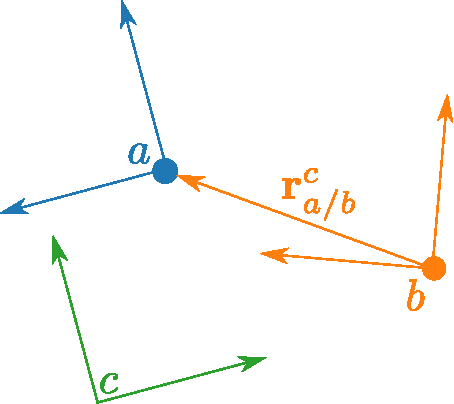
\includegraphics[width=\linewidth]{chap2_preliminaries/figures/frame}
\caption{Illustration of a vector with notation}
\label{fig:notation}
\end{marginfigure}

Although it may be sometimes hard to actually draw some quantities
clearly (like the angular rate of two coordinate frames), in engineering,
we typically define vectors as some quantity with respect to some
other reference. For example, the angular velocity of a rotating body
with respect to the earth might be written as $\omegabf_{b/E}$. While it
may be difficult to visualize, we could also consider the opposite
case, what the angular velocity of the earth was with respect to the
rotating body, $\omegabf_{E/b}$. It turns out that even in
this case, the ``earth-centric'' representation is just the negative
of the ``body-centric'' representation.
\[
\omegabf_{E/b}=-\omegabf_{b/E}.
\]

The next piece of information that we need is the frame of reference
it is described in (its basis). For example, in Figure~\ref{fig:notation},
we could describe $\rbf$ in any coordinate frame we want. We could
use frame $a$, $b$ or $c$, it doesn't really matter, so long as
we always do all operations between vectors represented in the same
frame.

We will use the superscript notation to describe the frame of reference,
as in $\rbf_{a/b}^{c}$.
\sidenote{In words $r_{a/b}^c$ means ``the position of frame $a$ with respect to
frame $b$, expressed in frame $c$.''} All vectors have this concept
of frame of reference, even if they are hard to visualize, like angular
rate, acceleration, etc...

%-------------------------------------------------------------
\subsection{A first look at rotation matrices.}
We can transform vector coordinates from one frame to another using a rotation matrix.  Let $R_a^b\in\mathbb{R}^{3\times 3}$ be the matrix that transforms the coordinates of physical vector expressed in frame $a$ to the coordinates of the same physical vector expressed in frame $b$.  
Note that $R_a^b$ will transform the coordinate axes of frame $a$ expressed in $a$ to the coordinate axes of frame $a$ expressed in $b$.  Therefore if we write $R_a^b$ in terms of its columns $R_a^b = \begin{pmatrix}\rbf_1 & \rbf_2 & \rbf_3 \end{pmatrix}$, then we have
\[
R_a^b \ibf_a^a =  \begin{pmatrix}\rbf_1 & \rbf_2 & \rbf_3 \end{pmatrix} \begin{pmatrix} 1 \\ 0 \\ 0 \end{pmatrix} 
= \rbf_1 
= \ibf_a^b.
\]
Using similar logic for the other columns we have
\[
R_a^b = \begin{pmatrix} \ibf_a^b & \jbf_a^b & \kbf_a^b \end{pmatrix}.
\]
\marginnote{The columns of the rotation matrix $R_a^b$ are the coordinate axes of frame $a$ expressed in frame $b$.}

Suppose that a vector $\rbf_{a/b}$ is expressed with respect to frame $c$ and we would like to express it with respect to frame $d$, then we can use the rotation matrix $R_c^d$ as the transformation
\[
\rbf_{a/b}^{d}=R_{c}^{d}\rbf_{a/b}^{c}
\]
\marginnote{The notation
is such that you can ``cancel out'' the frames, as in
\[
\rbf_{a/b}^{b}=R_{\cancel{c}}^{b}\mathbf{r}_{a/b}^{c}.
\]
Rotations can also be compounded as in 
\[
\rbf_{a/b}^{e}=R_{\cancel{d}}^{e}R_{\cancel{c}}^{\cancel{d}}\rbf_{a/b}^{\cancel{c}}.
\]
}
%
%Again, I'm deliberately skimming over most of the actual math. We'll
%get into this a lot more later, but we first need to get the mechanics
%of working with this notation.

%-----------------------------------------------------
\subsection{Vector composition.}
Recall that vector space is a collection of vectors and a scalar field with operations for vector addition and scalar multiplication.  The following table provides the definition for these operations.
%
%
%Let's now take a minute to remember what defines a vector space. From
%Wikipedia:
%\begin{quote}
%A vector space is a collection of objects called vectors, which may
%be added together and multiplied (\textquotedbl scaled\textquotedbl )
%by numbers, called scalars.
%\end{quote}
%All vector spaces abide by the following rules:
\begin{table}[ht]
\caption{Table of the rules of a Vector Space}
\begin{tabular}{cc}
\hline 
Axiom & Meaning\\
\hline 
\hline 
Associativity & $\abf+\left(\bbf+\cbf\right)=\left(\abf+\bbf\right)+\cbf$\\
\hline 
Commutativity & $\abf+\bbf=\bbf+\abf$
\\\hline 
Identity vector & 
	There exists a vector $\zerobf$ \\& 
	such that $\abf+\zerobf=\abf$ for \\&
	every vector in the space
\\\hline 
Inverse vector & 
	for every vector $\abf$, there is \\&
	 one and only one vector $-\abf$\\&
	such that \\&
	$\abf+\left(-\abf\right)=\zerobf.$
\\\hline 
distributivity of \\ scalar multiplication & 
	$\left(v+u\right)\abf=v\abf+u\abf$ \\&
	$v\left(\abf+\bbf\right)=v\abf+v\bbf$
\\\hline 
Identity scalar & $1\abf=\abf$\tabularnewline
\hline 
\end{tabular}
\end{table}

Physical vectors are part of the 3D Euclidian vector space $\mathbb{E}^3$ the scalar field being given by the real numbers $\mathbb{R}$.  This will be in contrast to rotation matrices that are not elements of a vector space.  Later in this chapter we will define the notion of a group, which will be much more useful in dealing with rotation matrices.

%
%\begin{flushleft}
%If you've taken a course in linear algebra, these will not be new
%to you. However, for me, up to this point, I had never worked with
%objects that were \emph{not }in a vector space, so the rules seemed
%obvious and redundant.
%\par\end{flushleft}

We like vector spaces because computers are well-suited for solving
linear algebra problems. There are high-performance BLAS libraries
(basic linear algebra subprograms) and methods for performing matrix
decompositions (SVD, LU, QR, Cholesky etc...) that allow us to solve
complicated problems quickly and accurately. 

It turns out that rotations and transformations do \emph{not} lie
in a vector space. This means that we end up performing manipulations
to get our problems into a vector space where we can use powerful
linear algebra techniques, and the distinction between vector spaces
and non-vector spaces will become very important.

\begin{marginfigure}
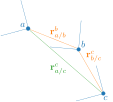
\includegraphics[width=\linewidth]{chap2_preliminaries/figures/vector_composition}
\caption{Illustration of a vector triangle}
\label{fig:vector_compose}
\end{marginfigure}
Figure~\ref{fig:vector_compose} shows three coordinate frames $a$, $b$, and $c$.
We would like to add the orange vectors $\rbf_{b/c}^c$ and $\rbf_{a/b}^b$.  
Vector addition applies, but only if the vectors are expressed in the same coordinate frame.  Therefore, to add the vectors we must first transform $\rbf_{a/b}^b$ into frame $c$ to get
\[
\rbf_{a/c}^{c}=\rbf_{b/c}^c + R_{b}^{c}\rbf_{a/b}^b.
\]
%
%
% as shown in Figure \ref{fig:vector_compose}.
%Let's also say that we have only the orange vectors. (the vector from
%$b\to a$ and the vector from $c\to b$) but we want the green vector
%(the one that goes all the way from $c\to a$).
%
%
%Well, this would be easy if they were all represented in the same
%coordinate frame
%
%\[
%\rbf_{a/c}=\rbf_{a/b}+\rbf_{b/c},
%\]
%but they aren't. However, we just have to remember that vectors can
%only be added or subtracted if they are in the same frame, so we just
%rotate them into a common frame before doing the additions, like this:
%
%\[
%\rbf_{a/c}^{c}=R_{b}^{c}\left(\rbf_{b/c}^{b}+R_{a}^{b}\rbf_{a/b}^{a}\right).
%\]
%From a theoretical perspective, the choice of coordinate frame doesn't
%matter, however in practice there is often a choice of frame that
%makes things easier.


%-----------------------------------------------------
\subsection{Cross product and skew symmetric matrices.}
The cross product of two vectors in $\mathbb{R}^3$ is defined as
\[
\begin{pmatrix} a_1 \\ a_2 \\ a_3 \end{pmatrix} \times \begin{pmatrix} b_1 \\ b_2 \\ b_3 \end{pmatrix} = \begin{pmatrix} a_2 b_3 - a_3 b_2 \\ a_3 b_1 - a_1 b_3 \\ a_1 b_2 - a_2 b_2 \end{pmatrix}.
\]
Direct manipulation shows that cross product satisfies the following identities:
\begin{align}
\abf \times \bbf = -\bbf \times \abf \label{eq:cross_product_1} \\
\abf \times (\bbf \times \cbf) = \abf^\top \cbf \bbf - \abf^\top\bbf \cbf \label{eq:cross_product_2} \\
\abf^\top(\bbf\times\cbf)=\cbf^\top(\abf\times\bbf)=\bbf^\top(\cbf\times\abf) \label{eq:cross_product_3} \\
(\abf\times\bbf)^\top(\cbf\times\dbf) = (\abf^\top\cbf)(\bbf^\top\dbf)-(\abf^\top\dbf)(\bbf^\top\cbf) \label{eq:cross_product_4} \\
\norm{\abf \times \bbf} = \norm{\abf}\norm{\bbf}\sin\phi, \quad \phi=\text{angle between $\abf$ and $\bbf$}\label{eq:cross_product_5} \\
\abf^\top (\bbf\times\cbf) = \text{det}\{\begin{pmatrix}\abf & \bbf & \cbf\end{pmatrix}\}. \label{eq:cross_product_6}
\end{align}
If $R$ is a rotation matrix, then 
\begin{equation} \label{eq:cross_product_7}
R(\abf\times\bbf) = (R\abf)\times(R\bbf).	
\end{equation}


It is straight forward to show that for any $\abf,\bbf\in\mathbb{R}^3$, 
\marginnote{The ``wedge'' operator is defined in Equation~\eqref{eq:wedge}.}  
\[
\ss{\abf}\bbf = \abf\times\bbf.
\]
Therefore $\ss{\abf}$ is a matrix implementation of the cross product operation.
From the properties of the cross product, we can derive the following properties for skew symmetric matrices:
\begin{align}
\ss{\abf} = -\ss{\abf}^\top \label{eq:skew_matrix_1}\\
\ss{\abf}\ss{\bbf} = \bbf\abf^\top - (\abf^\top\bbf)I \label{eq:skew_matrix_2}\\
\abf^\top\ss{\bbf} = (\ss{\abf}\bbf)^\top = -\bbf^\top\ss{\abf} \label{eq:skew_matrix_3}\\
(\ss{\abf}\bbf)^\top\ss{\cbf} = \abf^\top(\cbf\bbf^\top-\bbf^\top\cbf I).\label{eq:skew_matrix_4}
\end{align}
From property~\eqref{eq:skew_matrix_2}, we have that if $\nbf$ is a unit vector, then
\begin{equation}\label{eq:skew_matrix_5}
\ss{\nbf}^2 = \nbf\nbf^\top-I.
\end{equation}
\marginnote{
\begin{align*}
&R(\abf\times\bbf)=(R\abf)\times(R\bbf) \\
\iff & R\ss{\abf}\bbf = \ss{R\abf}R\bbf \\
\iff & R\ss{\abf} = \ss{R\abf}R \\
\iff & R\ss{\abf}R^\top = \ss{R\abf}
\end{align*}
}
From property~\eqref{eq:cross_product_7} we have
\begin{equation}\label{eq:skew_matrix_6}
\ss{R\abf} = R\ss{\abf}R^\top.
\end{equation}

Define the symmetric and skew-symmetric operators as
\begin{align}
\mathbb{P}_s (A) &\defeq \frac{1}{2}(A+A^\top) \label{eq:symmetric_operator} \\
\mathbb{P}_a (A) &\defeq \frac{1}{2}(A-A^\top), \label{eq:skew_symmetric_operator}
\end{align}
and note that $A=\mathbb{P}_s(A)+\mathbb{P}_a(A)$.  Therefore, any square matrix $A$ can be decomposed into a symmetric part, and a skew-symmetric part.

%++++++++++++++++++++++++++++++++++++++++++++++++++++++++++++
\subsection{Useful matrix identities}
In this section, we collect some useful matrix identities.

The trace of a matrix $A=\{a_{ij}\}\in\mathbb{R}^{m\times n}$ is defined as the sum of the the diagonal terms, i.e.,
\[
\trace{A} = \sum_{i=1}^{\min(m,n)} a_{ii}.
\]
The following properties of the trace of a matrix well known, where it is assumed that matrices have compatible dimensions:
\begin{align}
\trace{A^\top} =\trace{A}, \label{eq:trace_property_1} \\
\trace{AB} = \trace{BA}, \label{eq:trace_property_2} \\
\trace{\alpha A + \beta~B} = \alpha~\trace{A} + \beta~\trace{B}, \label{eq:trace_property_3} \\
A-\text{symmetric}, B-\text{skew symmetric} \implies \trace{AB} = 0, \label{eq:trace_property_4} \\
\trace{\ss{\abf} \ss{\bbf}} = -2\abf^\top \bbf. \label{eq:trace_property_5}
\end{align}


The Frobenius norm of matrix $A=\{a_{ij}\}\in\mathbb{R}^{n\times n}$ is defined as
\[
\norm{A}_F \defeq \sqrt{\trace{A^\top A}} = \sum_{ij} \abs{a_{ij}}^2.
\]
\begin{lemma} \label{lem:norm_to_trace}
If $R\in SO(3)$, then 
\begin{equation}\label{eq:frobenius_norm_to_trace}
\norm{I-R}_F^2 = 2~\trace{I-R}.
\end{equation}
\end{lemma}
\begin{proof}
\begin{align*}
\norm{I-R}_F^2 &= \trace{(I-R)^\top(I-R)} \\
  	&= \trace{I - R - R^\top + R^\top R}.
\end{align*}
Since $R\in SO(3)$ we have that $R^\top R = I$.  Therefore from properties~\eqref{eq:trace_property_1} and \eqref{eq:trace_property_3} we get Equation~\eqref{eq:frobenius_norm_to_trace}.
\end{proof}


%+++++++++++++++++++++++++++++++++++++++++++++++++++++++++++++
\section{The Rodrigues Formula}
\label{sec:rodrigues_formula}

In this section we derive the so-called {\em Rodrigues Formula} that describes a right handed rotation of angle $\theta$ about a vector $\mathbf{n}$. 
We will use this formula throughout the book. Our derivation
follows that given in {\em Stevens \& Lewis}~\cite{StevensLewis03}.  Consider the geometry shown in Figure~\ref{fig:rotation_formula}, where the vector $\mathbf{q}$ is obtained by a right-handed rotatation of the vector $\mathbf{p}$ about the unit vector $\mathbf{n}$ by an angle of $\theta$. 
%
\begin{marginfigure}[-5in]
  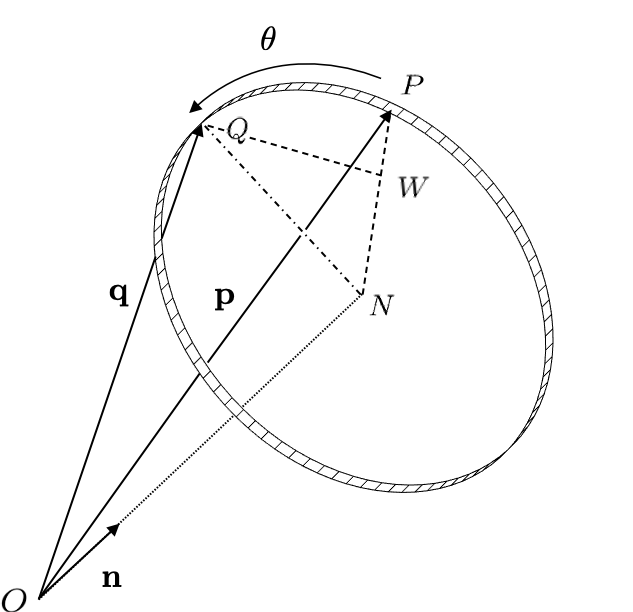
\includegraphics[width=\linewidth]{chap2_preliminaries/figures/rotation_formula}\\
  \caption{Right-handed rotation of a vector $\mathbf{p}$ about the unit
  vector $\mathbf{n}$ by an angle of $\theta$ to obtain the vector $\mathbf{q}$.}
  \label{fig:rotation_formula}
\end{marginfigure}
%
From the geometry, note that 
\begin{equation}\label{eq:frames-rot-formula-prelim}
\mathbf{q} = \vec{ON} + \vec{NW} + \vec{WQ}.
\end{equation}
The vector $\vec{ON}$ can be found by taking the projection of
$\mathbf{p}$ on the unit vector $\mathbf{n}$ in the direction of
$\mathbf{n}$, giving
\[
\vec{ON} = \left(\pbf\cdot\nbf\right)\nbf = (\nbf \nbf^\top) \pbf.
\]
The vector $\vec{NW}$ is in the direction of $\mathbf{p}-\vec{ON}$
with a length of $\norm{\vec{NQ}}\cos\theta$.  Noting that the length $NQ$ equals
the length $NP$ which is equal to $\norm{\mathbf{p}-\vec{ON}}$ we
get that
\begin{align*}
\vec{NW} &= \frac{\pbf-\left(\pbf \cdot \nbf\right)\nbf}
{\norm{\pbf-\left(\pbf\cdot\nbf\right)\nbf}}
\norm{\vec{NQ}}\cos\theta
\\
&=
\cos\theta\left(I-\nbf\nbf^\top\right)\pbf.
\end{align*}
The vector $\vec{WQ}$ is perpendicular to both $\mathbf{p}$ and
$\mathbf{n}$ and has length $\norm{\vec{NQ}}\sin\theta$.  Noting that
$\norm{\vec{NQ}}=\norm{\mathbf{p}}\sin\phi$ and that $\norm{\nbf\times\pbf}=\norm{\pbf}\sin\phi$, where $\phi$ is the angle between $\nbf$ and $\pbf$, we get
\begin{align*}
\vec{WQ} &=
\frac{\nbf\times\pbf}{\norm{\nbf\times\pbf}}\norm{\vec{NQ}}\sin\theta
\\
&= \mathbf{n}\times\mathbf{p}\sin\theta \\
&= \sin\theta \ss{\nbf}\pbf.
\end{align*}
Therefore Equation~\eqref{eq:frames-rot-formula-prelim} becomes
\[
\mathbf{q} = \left(\nbf \nbf^\top + \cos\theta (I-\nbf\nbf^\top) + \sin\theta \ss{\nbf} \right)\pbf.
\]
Let
\[
R(\nbf,\theta)=\nbf \nbf^\top + \cos\theta (I-\nbf\nbf^\top) + \sin\theta \ss{\nbf},
\]
and note that using Equation~\eqref{eq:skew_matrix_5} we can write
\marginnote{Equation~\eqref{eq:skew_matrix_5} is $(\ss{\nbf})^2 = \nbf\nbf^\top-I$.}
\begin{equation}\label{eq:rodrigues_1}
R(\nbf,\theta)=I + \sin\theta \ss{\nbf} + (1-\cos\theta)\ss{\nbf}^2,
\end{equation}
which is called the Rodrigues formula.
As described in the next section, we will often use angle-axis notation to define rotations.  In angle-axis notation, the rotation vector is given by
$\abf=\theta\nbf$.  Therefore, we will typically write the Rodrigues formula as 
\begin{equation}\label{eq:rodigues_2}
	R(\theta\nbf) = I + \sin\theta \ss{\nbf} + (1-\cos\theta)\ss{\nbf}^2.
\end{equation}
Note that for any vector $\abf$ we have $\abf=\norm{\abf}\frac{\abf}{\norm{\abf}}$.  Equating $\theta$ with $\norm{\abf}$ and $\nbf$ with the unit vector $\abf/\norm{\abf}$, the Rodrigues formula becomes
\marginnote{We have used the identity $1-\cos x = 2\sin^2(x/2)$ to get $\frac{1-\cos x}{x^2} = \frac{1}{2}\sinc^2(x/2)$, where $\sinc(x)=\frac{\sin(x)}{x}$.}
\begin{align}
R(\abf) &= I + \left(\frac{\sin\norm{\abf}}{\norm{\abf}}\right)\ss{\abf} + \left(\frac{1-\cos\norm{\abf}}{\norm{\abf}^2}\right)\ss{\abf}^2 \notag \\
		&= I + \sinc(\norm{\abf})\ss{\abf} + \frac{1}{2}\sinc^2\left(\frac{\norm{\abf}}{2}\right)\ss{\abf}^2.
		\label{eq:rodrigues_2}
\end{align}

As an illustration of the Rodrigues formula, we get that a rotation of $\phi$ about the vector $\ebf_1=(1,0,0)^\top$ is
\begin{align*}
R(\ebf_1,\phi) &= I + \sin\phi \ss{\ebf} + (1-\cos\phi)\ss{\ebf_1}^2	\\
&= \begin{pmatrix}1 & 0 & 0 \\ 0 & 1 & 0 \\ 0 & 0 & 1 \end{pmatrix}
   +\sin\phi \begin{pmatrix} 0 & 0 & 0 \\ 0 & 0 & -1 \\ 0 & 1 & 0\end{pmatrix} 
   + (1-\cos\phi)\begin{pmatrix}0 & 0 & 0 \\ 0 & -1 & 0 \\ 0 & 0 & -1 \end{pmatrix} \\
&= \begin{pmatrix} 1 & 0 & 0 \\ 0 & \cos\phi & -\sin\phi \\ 0 & \sin\phi & \cos\phi \end{pmatrix}.
\end{align*}
Similarly, the Rodrigues formula gives that rotations by $\theta$ about $\ebf_2$ and $\psi$ about $\ebf_3$ are
\begin{align*}
R(\ebf_2, \theta) &= \begin{pmatrix} \cos\theta & 0 & \sin\theta \\ 0 & 1 & 0 \\ -\sin\theta & 0 & \cos\theta \end{pmatrix} \\
R(\ebf_3, \psi) &= \begin{pmatrix} \cos\psi & -\sin\psi & 0 \\ \sin\psi & \cos\psi & 0 \\ 0 & 0 & 1 \end{pmatrix} \\
\end{align*}

One may wonder if all rotation can be described by the Rodrigues formula.  It turns out that Leonhard Euler proved in 1775 the following theorem.
\sidenote{\url{https://en.wikipedia.org/wiki/Euler\%27s_rotation_theorem}.}
\begin{theorem}[Euler's Rotation Theorem]
	In three dimensional space, any sequence of rotations is equivalent to a single rotation about a fixed vector.
\end{theorem}
Therefore, any rotation and any sequence of rotations, can be represented by a single rotation matrix with some angle $\theta$ and some unit vector $\nbf$, where the corresponding rotation is $R(\nbf,\theta)$.
It turns out that the eigenvalues and eigenvectors of any rotation $R(\nbf,\theta)$ can be derived analytically.
\begin{lemma}
Given a rotation matrix $R(\nbf,\theta)$ the eigenvalues are $\lambda=1, \exp(j\theta), \exp(-j\theta)$, with corresponding eigenvectors
$\nbf$, $\nbf_2+j\nbf_3$, and $\nbf_2-j\nbf_3$, where $\{\nbf, \nbf_2, \nbf_3\}$ form a right handed coordinate frame.
\end{lemma}
\begin{proof}
From the Rodrigues formula we get
\marginnote{We have used the fact that $\nbf\times\nbf=0$ implies that $\ss{\nbf}\nbf = 0$.}
\[
R(\nbf,\theta)\nbf = \nbf + \sin\theta \ss{\nbf}\nbf + (1-\cos\theta)\ss{\nbf}\ss{\nbf}\nbf
                   = 1\cdot\nbf.
\]
Therefore $\lambda=1$ is an eigenvector of $R(\nbf,\theta)$ with eigenvector $\nbf$.  Pick any $\nbf_2$ that is orthogonal to $\nbf$, and let $\nbf_3=\ss{\nbf}\nbf_2$ so that $\{\nbf, \nbf_2, \nbf_3\}$ form a right-handed coordinate system.  Then
\begin{align*}
	R(\nbf,\theta)\nbf_2 &= \nbf_2 + \sin\theta \ss{\nbf}\nbf_2 + (1-\cos\theta)\ss{\nbf}\ss{\nbf}\nbf_2 \\
	&= \nbf_2 + \sin\theta \nbf_3 - (1-\cos\theta)\nbf_2 \\
	&= \cos\theta \nbf_2 + \sin\theta \nbf_3.
\end{align*}
Similarly, it is straightforward to show that $R(\nbf,\theta)\nbf_3 = \cos\theta \nbf_3 - \sin\theta \nbf_2$.  Therefore
\begin{align*}
	R(\nbf,\theta)(\mathbf{n}_2 \pm j\mathbf{n}_3) &= (\cos\theta\mathbf{n}_2 + \sin\theta\mathbf{n}_3) \pm j(\cos\theta \mathbf{n}_3 - j\sin\theta\mathbf{n}_2) \\
		&= (\cos\theta \pm j\sin\theta)\mathbf{n}_2 \mp j(\cos\theta \pm j\sin\theta)\mathbf{n}_3 \\
		&= e^{\pm j\theta} (\mathbf{n}_2 \mp j\mathbf{n}_3).
\end{align*}
Therefore, the other two eigenvectors are $\mathbf{n}_2\pm j\mathbf{n}_3$ with associated eigenvalues of $e^{\mp j\theta}$.  
Conversely, it can be shown that all rotation matrices have a similar eigen-structure.  Therefore, every rotation matrix $R\in SO(3)$ will have eigenvalues of $1$ and $e^{\mp j\theta}$, and $R$ can be visualized as rotating a vector $\mathbf{p}$ by a left-handed rotation of angle $\theta$ about the eigenvector $\mathbf{n}$ associated with eigenvalue $1$. 
\end{proof}
It is standard convention to call $\nbf$ the eigen-axis of rotation.  

The Rodrigues formula also gives the following result for the trace of $R$.
\begin{lemma}\label{lem:prelim-trace-of-R}
For any $R(\nbf,\theta)\in SO(3)$ we have
\[
\trace{R} = 1+2\cos\theta.
\]	
\end{lemma}
\begin{proof}
Since $\ss{\nbf}^2 = \nbf \nbf^\top  - I$, we get that
\begin{align*}
\trace{R} &= \trace{I} + \sin\theta~\trace{\ss{\nbf}} + (1-\cos\theta)\trace{\nbf \nbf^\top - I} \\
          &= 3 + \sin\theta \cdot 0 + (1-\cos\theta)(n_1^2+n_2^2+n_3^2 - 3) \\
          &= 1 + 2\cos\theta,
\end{align*}
where $\nbf=(n_1, n_2, n_3)^\top$.
\end{proof}

We conclude this section by deriving an extremely useful expression for the Rodrigues formula.  Recall from linear algebra, that the exponential of a square matrix $A\in\mathbb{R}^{n\times n}$ is defined as
\begin{equation}\label{eq:matrix_exponential}
e^{A} = \exp(A) = I + A + \frac{1}{2!}A^2 + \frac{1}{3!}A^3 + \frac{1}{4!}A^4 + \dots.
\end{equation}
\begin{lemma}\label{lem:rodrigues_exponential}
For any unit vector $\nbf$ and scalar $\theta$,
\[
R(\nbf,\theta) = \exp(\theta\ss{\nbf}).
\]	
\end{lemma}
\begin{proof}
From Equation~\eqref{eq:skew_matrix_5} we have that
\begin{align*}
	\ss{\nbf}^3 &= \ss{\nbf}(\nbf\nbf^\top-I) \\
	            &= -\ss{\nbf},
\end{align*}
implying that for $m=0, 1, 2, \dots$, $\ss{\nbf}^{(2m+1)} = (-1)^m\ss{\nbf}$.
Therefore $\ss{\nbf}^4=-\ss{\nbf}^2$, implying that for $m=0, 1, 2, \dots$, 
$\ss{\nbf}^{(2m+2)} = (-1)^m\ss{\nbf}^2$. Using Equation~\eqref{eq:matrix_exponential} we get
\begin{align*}
\exp(\theta \ss{\nbf}) &= I + \theta \ss{\nbf} + \frac{\theta^2}{2!}\ss{\nbf}^2 + \frac{\theta^3}{3!}\ss{\nbf}^3 + \frac{\theta^4}{4!}\ss{\nbf}^4
                          + \dots \\
                      &= I + \theta \ss{\nbf} + \frac{\theta^2}{2!}\ss{\nbf}^2 - \frac{\theta^3}{3!} \ss{\nbf} - \frac{\theta^4}{4!}\ss{\nbf}^2 +\dots \\
                      &= I + \left(\theta - \frac{\theta^3}{3!} + \frac{\theta^5}{5!} - \dots \right)\ss{\nbf} + \left(\frac{\theta^2}{2!} - \frac{\theta^4}{4!} + \dots\right)\ss{\nbf}^2 \\
                      &= I + \sin\theta\ss{\nbf} -(\cos\theta -1)\ss{\nbf}^2 \\
                      &= R(\nbf, \theta).
\end{align*}
\end{proof}

We can also define the $\log$ of a rotation matrix as the inverse operation, where we require that $\log(\exp(R))=R$.
\begin{lemma}\label{lem:matrix_log}
Given any $R\in SO(3)$, the logarithm of $R$ is given by
\[
\log(R) = \frac{1}{2}\frac{R-R^\top}{\sinc{\theta}}
\]
where
\[
\theta = \cos^{-1}\left(\frac{\trace{R}-1}{2}\right).
\]
%\[
%\log(R) = \left(\frac{\cos^{-1}\left(\frac{\trace{R}-1}{2}\right)}{\sqrt{(3-\trace{R})(1+\trace{R})}}\right)(R-R^\top).
%\]
\end{lemma}
\begin{proof}
Euler's rotation theorem implies that there exist $\nbf$ and $\theta$ such that $R=\exp(\theta\ss{\nbf})$.  Therefore
\[
\log(R) = \log(\exp(\theta\ss{\nbf}))=\theta\ss{\nbf}.
\]
From Lemma~\ref{lem:prelim-trace-of-R} we have that
\[
\theta = \cos^{-1}\left(\frac{\trace{R}-1}{2}\right).
\]
Using the Rodrigues formula we have
\sidenote{We have used the fact that $\ss{\nbf}^\top = -\ss{\nbf}$ and $\ss{\nbf}^{\top 2} = \ss{\nbf}^2$.}
\begin{align*}
R - R^\top &= I + \sin\theta \ss{\nbf} + (1-\cos\theta)\ss{\nbf}^2 \\
		   &\qquad - I^\top - \sin\theta\ss{\nbf}^\top - (1-\cos\theta)\ss{\nbf}^{\top 2} \\
           &= 2\sin\theta \ss{\nbf},
\end{align*}
which implies that \sidenote{Note that this formula shows that an equivalent expression for the logarithm or $R$ is $\log(R) = \frac{1}{2}\frac{R-R^\top}{\sinc\theta}$ where $\sinc\theta = \frac{\sin\theta}{\theta}$.}
\[
\ss{\nbf} = \frac{R-R^\top}{2\sin\theta}.
\]
Therefore
\[
\log{R} = \theta\ss{\nbf} = \theta\frac{R-R^\top}{2\sin\theta} = \frac{1}{2}\frac{R-R^\top}{\sinc{\theta}}.
\]
%
%Using the fact that $\sin(\cos^{-1}(x))=\sqrt{1-x^2}$ gives
%\[
%\sin\left(\cos^{-1}\left(\frac{\trace{R}-1}{2}\right)\right) = \frac{\sqrt{(3-\trace{R})(1+\trace{R})}}{2},
%\]
%which gives the result.
\end{proof}


%-------------------------------------------------------------
\section{Attitude Representation}
\label{sec:attitude_representation}

In this section we describe four different attitude representations that will be used in the book.  The attitude or orientation of a multirotor can be described using Euler angles, a rotation matrix, a unit quaternion, or using a rotation vector, which is often called angle-axis representation.  The following subsection will describe each of these conventions and how they are used to describe the attitude of a multirotor, and the attitude of an attached camera.  We will find that each of these representations are convenient for different aspects of vision-based estimation and control, and so we also describe how to transform between the different representations.

%+++++++++++++++++++++++++++++++++++++++++++++++++++++++++++++
\subsection{Euler Angles}

The most common representation for attitude is the 3-2-1 Euler angles, often called the aircraft yaw, pitch, and roll angles.  
The body frame of a multirotor is defined as $\mathcal{F}_b = \{\ibf_b, \jbf_b, \kbf_b\}$.  The body $\ibf_b$-axis is in a plane parallel to the rotors, and points in a direction that is designated as the forward-direction for the multirotor. The body $\kbf_b$-axis is perpendicular to the rotor plane, and points opposite the direction of thrust, designated as the body down direction.  The body $\jbf_b$-axis is so that $\jbf=\kbf\times\ibf$ and points to the right in the body.

The yaw angle of a multirotor is defined as a right-handed rotation about the inertial $\kbf_i$ axis, as shown in Figure~\ref{fig:quadrotor_yaw}.  The resulting intermediary frame is called the body-1 frame in \cite{BeardMcLain12}.  The yaw angle is designated as $\psi$.
\begin{marginfigure}
  \centering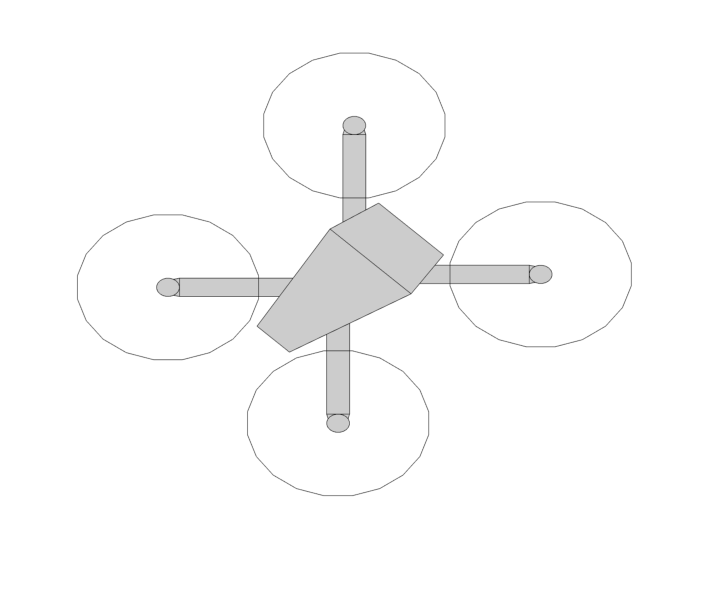
\includegraphics[width=\linewidth]{chap2_preliminaries/figures/quadrotor_yaw}
  \caption{The yaw angle is defined as a right-handed rotation about the inertial $\kbf_i$ axis.}
  \label{fig:quadrotor_yaw}  
\end{marginfigure}
%
The pitch angle of a multirotor is defined as a right-handed rotation about the $\jbf_1$ in the body-1 frame, as shown in Figure~\ref{fig:quadrotor_pitch}, and the resulting intermediary frame is called the body-2 frame in~\cite{BeardMcLain12}. The pitch angle is designated as $\theta$.
\begin{marginfigure}
  \centering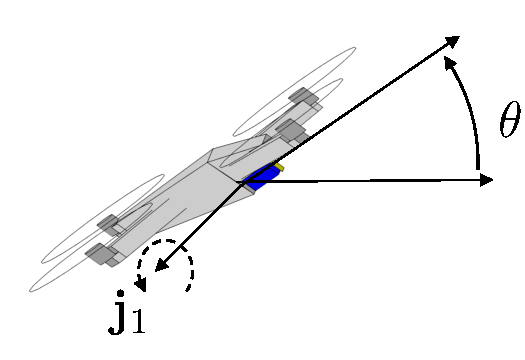
\includegraphics[width=\linewidth]{chap2_preliminaries/figures/quadrotor_pitch}
  \caption{The pitch angle is defined as a right-handed rotation about the body-1 $\jbf$ axis.}
  \label{fig:quadrotor_pitch}  
\end{marginfigure}
%
The roll angle of a multirotor is defined as a right-handed rotation about the body-2 $\ibf_2$ axis, as shown in Figure~\ref{fig:quadrotor_roll}.  The roll angle is designated as $\phi$.
\begin{marginfigure}
  \centering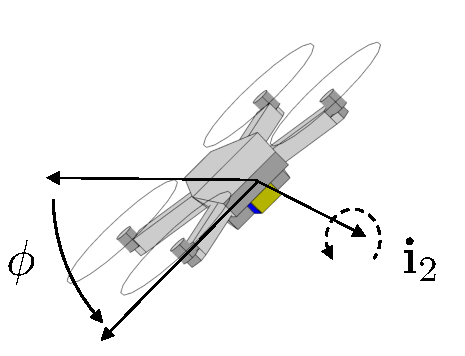
\includegraphics[width=\linewidth]{chap2_preliminaries/figures/quadrotor_roll}
  \caption{The roll angle is defined as a right-handed rotation about the body-2 $\ibf_2$ axis.}
  \label{fig:quadrotor_roll}  
\end{marginfigure}
Throughout the book, we will designate the vector of Euler angles by 
\[
\Theta = \begin{pmatrix} \phi \\ \theta \\ \psi \end{pmatrix}.
\]

Euler angle are often used because they are intuitive to understand and easy to visualize.  When attitude needs to be plotted in a graph, the Euler angles are typically used for convenience.  However, Euler angles represent a local representation of attitude and are rarely suitable for simulation, estimation, or control.  First note that Euler angles do not commute, i.e., a yaw followed by a pitch followed by a roll, is different than a roll followed by a pitch followed by a yaw.  This non-commutivity has many negative implications.  To understand that they are a local representation, consider the attitude that would result by first pitching the multirotor by 90 degrees, and then rolling by 90 degrees.  This is the same orientation that would result from first yawing by 90 degrees, and then pitching by 90 degrees.  Therefore Euler angle representations do not uniquely represent the attitude.


The pointing angle, or attitude of the camera relative to the multirotor can be describe by the azimuth and elevation angles.  
%
The azimuth angle of the camera is defined as a right-handed rotation about the multirotor body $\kbf_b$ axis, as shown in Figure~\ref{fig:quadrotor_azimuth}.  The resulting intermediary frame is called the gimbal-1 frame in \cite{BeardMcLain12}.  The azimuth angle is designated in this book as $\alpha$.
\begin{marginfigure}
  \centering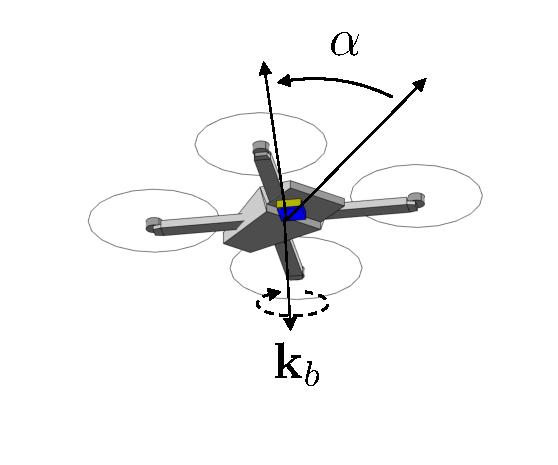
\includegraphics[width=\linewidth]{chap2_preliminaries/figures/quadrotor_azimuth}
  \caption{The azimuth angle of the camera is defined as a right-handed rotation about the multirotor body $\kbf_b$ axis.}
  \label{fig:quadrotor_azimuth}  
\end{marginfigure}
%
The elevation angle of the camera is defined as a right-handed rotation about the gimbal-1 $\jbf_{g1}$ axis, as shown in Figure~\ref{fig:quadrotor_elevation}.  The resulting frame is called the gimbal frame.  The elevation angle is designated in this book as $\beta$.
\begin{marginfigure}
  \centering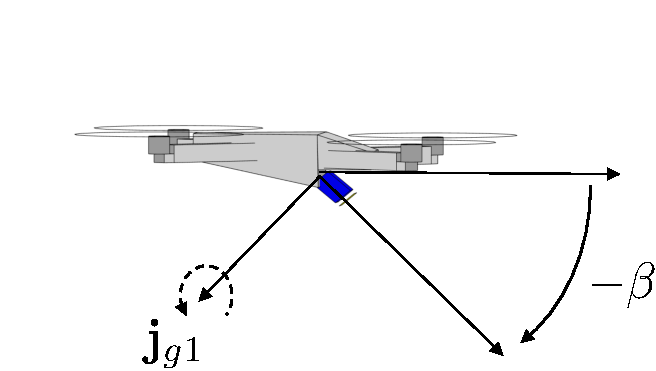
\includegraphics[width=\linewidth]{chap2_preliminaries/figures/quadrotor_elevation}
  \caption{The elevation angle of the camera is defined as a right-handed rotation about the gimbal-1 $\jbf_{g1}$ axis.}
  \label{fig:quadrotor_elevation}  
\end{marginfigure}


\subsection{Rotation Matrices}

As discussed previously, the attitude of a multirotor can also be represented by a rotation matrix.
A matrix $M\in\mathbb{R}^{n\times n}$ is said to be {\em orthogonal} if $MM^\top = M^\top M=I$, or equivalently if $M^{-1} = M^\top$.  The set of $n$-dimensional orthogonal matrices are designated by 
\[
O(n) = \{ M\in\mathbb{R}^{n\times n} | M^{-1}=M^\top \}.
\]
If $M=(\mbf_1, \mbf_2, \dots, \mbf_n)\in O(n)$, then 
\[
M^\top M =\begin{pmatrix} \mbf_1^\top \mbf_1 & \dots & \mbf_1^\top \mbf_n \\
\vdots & & \vdots \\
\mbf_n^\top \mbf_1 & \dots & \mbf_n^\top \mbf_n \end{pmatrix}=I
\]
implies that the columns of $M$ are orthogonal to each other and have unit length.  From properties of the determinate $\text{det}(M^\top)=\text{det}(M)$ and $\text{det}(I)=1$, we have that
\begin{align*}
& \text{det}(M^\top M) = \text{det}(I) \\
\iff & \text{det}^2(M) = 1 \\
\iff & \text{det}(M) = \pm 1.	
\end{align*}
For $3\times 3$ matrices, Equation~\eqref{eq:cross_product_6} implies that $\text{det}(M)=\mbf_1^\top(\mbf_2\times\mbf_3)$.  Therefore $\text{det}(M)=1$ if and only if the columns of $M$ form a right-handed coordinate system ($\mbf_2\times\mbf_3=\mbf_1$), otherwise the determinant is equal to $-1$.  
Therefore we define the set of special orthogonal matrices 
\[
SO(n) = \{M\in\mathbb{R}^{n\times n} | M\in O(n) \text{~and~} \text{det}(M)=1 \},
\]
and note that $R\in SO(3)$ implies that the columns of $R$ form a right-handed coordinate system.  Therefore, there is a one-to-one relationship between the orientation of right-handed coordinate systems and elements of $SO(3)$.  We say that $R$ is a rotation matrix if $R\in SO(3)$.  Note that the set $SO(3)$ does not form a vector space since $aR_1+bR_2\not\in SO(3)$ when $R_1,R_2\in SO(3)$.  We will see later that elements of $SO(3)$ form a {\em group}, and which is called the {\em special orthgonal group of order 3}.

Therefore, the orientation of a multirotor can be represented by an element of $SO(3)$.  If $\mathcal{F}_b = \{\ibf_b, \jbf_b, \kbf_b\}$ is a right-handed coordinate frame fixed in the multirotor body, then the attitude of $\mathcal{F}_b$ relative to another frame $\mathcal{F}_a = \{\ibf_a, \jbf_a, \kbf_a\}$ is given by
\[
R_b^a = \begin{pmatrix} \ibf_b^a & \jbf_b^a & \kbf_b^a \end{pmatrix}
\]
where the columns of $R_a^b$ are the unit vectors of frame $\mathcal{F}_b$ expressed relative to frame $\mathcal{F}_a$.  We will be particularly interested in $R_b^i$, the attitude of the multirotor body relative to the inertial frame, where $\ibf_b$ points out the nose of the multirotor, $\jbf_b$ points to the right, and $\kbf_b$ points down.  

To represent the attitude of the gimbal relative to the body, we need to assign a right-handed coordinate system to the gimbal.  Define $\mathcal{F}_g = \{\ibf_g, \jbf_g, \kbf_g\}$ such that $\ibf_g$ points along the optical axis of the camera, $\kbf_g$ points down when the gimbal is level, and $\jbf_g = \kbf_g\times\ibf_g$ points to the right.  The attitude of the gimbal relative to the body is given by
\[
R_g^b = \begin{pmatrix} \ibf_g^b & \jbf_g^b & \kbf_g^b \end{pmatrix}.
\]

To gain further insights into rotation matrices, note that any vector $\pbf$ can be represented in $\mathcal{F}_r$ and $\mathcal{F}_s$ as
\[
\pbf = \alpha_r\ibf_r + \beta_r\jbf_r + \gamma_r\kbf_r = \alpha_s\ibf_s + \beta_s\jbf_s + \gamma_s\kbf_s.
\]
Taking the inner product of both sides of this equation with the vectors $\ibf_r$, $\jbf_r$, and $\kbf_r$ gives
\begin{align*}
\alpha_r &= \alpha_s\ibf_r^\top \ibf_s + \beta_s\ibf_r^\top\jbf_s + \gamma_s\ibf_r^\top\kbf_s \\	
\beta_r &= \alpha_s\jbf_r^\top \ibf_s + \beta_s\jbf_r^\top\jbf_s + \gamma_s\jbf_r^\top\kbf_s \\
\gamma_r &= \alpha_s\kbf_r^\top \ibf_s + \beta_s\kbf_r^\top\jbf_s + \gamma_s\kbf_r^\top\kbf_s.
\end{align*}
Since $\pbf^r=(\alpha_r, \beta_r, \gamma_r)^\top$ and $\pbf^s=(\alpha_s, \beta_s, \gamma_s)^\top$ we have 
\[
\begin{pmatrix} \alpha_r \\ \beta_r \\ \gamma_r  \end{pmatrix} = 
\begin{pmatrix}
	\ibf_r^\top \ibf_s & \ibf_r^\top\jbf_s & \ibf_r^\top\kbf_s \\	
    \jbf_r^\top \ibf_s & \jbf_r^\top\jbf_s & \jbf_r^\top\kbf_s \\
    \kbf_r^\top \ibf_s & \kbf_r^\top\jbf_s & \kbf_r^\top\kbf_s
\end{pmatrix}
\begin{pmatrix}
	\alpha_s \\ \beta_s \\ \gamma_s
\end{pmatrix},
\]
\marginnote{The Cauchy-Schwartz equalty says that for any two vectors $\abf$ and $\bbf$, $\abf^\top \bbf = \norm{\abf}\norm{\bbf}\cos\theta$ where $\theta$ is the angle between $\abf$ and $\bbf$.}
or in other words $\pbf^r = R_s^r \pbf^s$, where we see that since $\nbf^\top\mbf=\cos\theta$ where $\theta$ is the angle between $\nbf$ and $\mbf$, that $R_s^r$ is a matrix of cosines of angles between the unit vectors of frame $r$ and frame $s$.  Therefore, rotation matrices are often called {\em direction cosine matrices.}  Therefore the vector
\[
\ibf_s^r = \begin{pmatrix}
 \text{angle between $\ibf_s$ and $\ibf_r$} \\	
 \text{angle between $\ibf_s$ and $\jbf_r$} \\	
 \text{angle between $\ibf_s$ and $\kbf_r$} \\	
 \end{pmatrix}.
\]

To emphasize some of the concept above, let $\mathcal{R}_r = \{\ibf_r, \jbf_r, \kbf_r\}$ and let $\mathcal{R}_s = \{\ibf_s, \jbf_s, \kbf_s\}$, 
then note that 
\[
\ibf_s^s = \begin{pmatrix} 1 \\ 0 \\ 0 \end{pmatrix}, \qquad 
\jbf_s^s = \begin{pmatrix} 0 \\ 1 \\ 0 \end{pmatrix}, \qquad 
\kbf_s^s = \begin{pmatrix} 0 \\ 0 \\ 1 \end{pmatrix}.
\]
Given the discussion above we have that
\[
R_s^r = \begin{pmatrix} \ibf_s^r & \jbf_s^r & \kbf_s^r \end{pmatrix},
\]
or 
\[
\ibf_s^r = R_s^r \ibf_s^s = \begin{pmatrix} \ibf_s^r & \jbf_s^r & \kbf_s^r \end{pmatrix} \begin{pmatrix} 1 \\ 0 \\ 0 \end{pmatrix}.
\]
Therefore the columns of $R_s^r$ are the unit axes of frame $\mathcal{F}_s$ expressed with respect to frame $\mathcal{F}_r$.

Let $\pbf_q$, $\pbf_r$ and $\pbf_s$ be the coordinates of $\pbf$ when expressed with respect to frames $\mathcal{F}_q$, $\mathcal{F}_r$, and $\mathcal{F}_s$, respectively. Then we can write
\begin{align*}
\pbf^r &= R_s^r \pbf^s \\
\pbf^q &= R_r^q \pbf^r.
\end{align*}
Therefore we have that $\pbf^q = R_r^q R_s^r \pbf^s$.  Since we also know that $\pbf_q = R_s^q \pbf_s$, we must have that
\[
R_s^q = R_r^q R_s^r.
\]

We have shown that rotation matrices satisfy the following properties
\begin{align}
& (R_r^s)^{-1} = (R_r^s)^T = R_s^r \label{eq:rotations_matrics_1} \\
& R_r^q R_s^r = R_s^q \label{eq:rotations_matrics_2} \\
& \det{R_r^s} = 1. \label{eq:rotations_matrics_3}
\end{align}

%+++++++++++++++++++++++++++++++++++++++++++++
\subsection{Passive Versus Active Rotations}

\begin{marginfigure}[-7in]
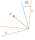
\includegraphics[width=0.8\linewidth]{chap2_preliminaries/figures/rotation_passive}
\caption{Illustration of a passive rotation.}
\label{fig:passive_rotation}
\end{marginfigure}

\begin{marginfigure}[-3in]
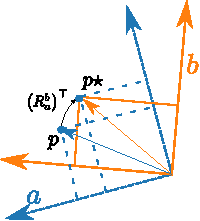
\includegraphics[width=0.8\linewidth]{chap2_preliminaries/figures/rotation_active}
\caption{Illustration of an active rotation.}
\label{fig:active_rotation}
\end{marginfigure}

We are using a convention here, where we define $R$ as a \emph{passive}
rotation. Consider Equation \ref{eq:rot_formula}. The vector quantity
$\rbf$ did not change during this rotation, it is simply being expressed
from another point of view. Some literature defines rotations as \emph{active}.
Figures~\ref{fig:passive_rotation} and~\ref{fig:active_rotation} illustrates the difference between
active and passive rotations. In the passive case, the point
$p$ does not change when rotating from frame $a$ to $b$. It remains
fixed while the perspective changes. In contrast, the active case, the point $p$ is moved to become a new object, point $\pbf^{\star}$.
This interpretation is much more common in the computer graphics literature,
where a common operation is to generate some asset at an arbitrary
origin, and then move that object to be rendered at some other location.
Engineering and robotics literature typically deal with passive rotations,
where the goal is often to reason about physical entities that are
not always directly controlled.

It can be shown that active and passive rotations are the transpose of
one another, as
\[
R_{active}=R_{passive}^{\top}.
\]
Throughout the book, we will always use passive rotations unless otherwise stated.

While rotation matrices are probably the most straight-forward method
to represent rotations, they have some shortcomings. The first is
that they require nine parameters to describe three degrees of freedom. This
causes larger memory requirements than strictly necessary, and requires
more operations than necessary when concatenating matrices.  With modern
computing resources, this is less of a problem, however the biggest
disadvantage is that numerical errors can accumulate in rotation matrices
and cause unwanted scaling and shearing as the matrix loses orthonormality.
This error can be corrected by Gram-Schmidt orthogonalization, but
doing so can be computationally expensive. As a result, rotation matrices
are still much more efficient than an Euler angle representation,
but they are not as efficient as unit quaternions.


%+++++++++++++++++++++++++++++++++++++++++++++++++++++++++++++
\subsection{Quaternions}

The material in this section loosely follows the notation in~\cite[-3in]{TrawnyRoumeliotis05}.

One of the disadvantages of rotation matrices is that they require nine parameters to represent a rotation, which is fundamentally a three dimensional entity.  Unit quaternions can be used to represent rotations using four parameters.  
Quaternions are hyper-complex numbers of the form 
\[
\mathbf{q} = q_0 + i q_x + j q_y + k q_z,
\]
where $i$, $j$, and $k$ are generalized complex numbers that satisfy 
\begin{equation}\label{eq:quaternion-complex-numbers}
i^2 = j^2 = k^2 = ijk = -1.
\end{equation}
\marginnote[-3in]{Because of the reverse order of concatenation, there is actually another
convention for quaternions, first used by NASA JPL, where the quaternion
imaginary numbers follow the \emph{left-hand} rule instead of the
right hand rule. This change makes unit quaternions concatenate right-to-left
(to match rotation matrices). The left-handed definition is known
as JPL notation, whereas the right-handed definition presented here
is known as Hamilton notation. While this change may seem innocent
on the surface, it has huge implications when we start talking about
Lie Groups. Modern scientific literature in robotics and computer
vision that use quaternions seem to almost always use Hamilton notation,
although JPL is used in some early quaternion papers relating to spacecraft
attitude observers.}

Equation~\eqref{eq:quaternion-complex-numbers} implies that $ijk^2=-k$ which implies that $ij=k$, which implies that $ij^2=kj$, which implies that $kj=-i$.  
By similar arguments we can show that $ij=-ji=k$, $jk=-kj=i$ and $ki=-ik=j$
Letting $\mathbf{p}=p_0 + ip_x + jp_y + kp_z$, we can multiply $\mathbf{p}$ and $\mathbf{q}$, and use the above relationships for $i, j, k$ to get
\begin{align}
\mathbf{p}\mathbf{q} &= (p_0 + ip_x + jp_y + kp_z)(q_0 + i q_x + j q_y + k q_z) \notag \\
&= (p_0q_0-p_xq_x-p_yq_y-p_zq_z) 
	+i(p_0q_x + p_xq_0 + p_yq_z - p_zq_y)
\\ &\quad
	+j(p_0q_y - p_xq_z + p_yq_0 + p_zq_x)
	+k(p_0q_z + p_xq_y - p_yq_x + p_zq_0)
\label{eq:quaternion-product-pre}
\end{align}

Throughout this book we will denote quaternions as a four vector
\[
\mathbf{q} = \begin{pmatrix} q_0 \\ \bar{q} \end{pmatrix},
\]
where $q_0$ is called the scalar part of the quaternion, and $\bar{q} = (q_x, q_y, q_z)^\top$, representing the complex elements, is called the vector part of the quaternion.  In vector notation, the quaternion product in Equation~\eqref{eq:quaternion-product-pre} becomes
\begin{align}
\mathbf{p}\otimes\mathbf{q} &= \begin{pmatrix} p_0 & -\bar{p}^\top \\ \bar{p} & p_0I + \ss{\bar{p}} \end{pmatrix}\begin{pmatrix}q_0 \\ \bar{q}\end{pmatrix} \label{eq:quaternion_multiplication_1}\\
&= \begin{pmatrix} q_0 & -\bar{q}^\top \\ \bar{q} & q_0I-\ss{\bar{q}} \end{pmatrix}\begin{pmatrix}p_0 \\ \bar{p}\end{pmatrix}.
\label{eq:quaternion_multiplication_2}
\end{align}

It turns out that attitude can be represented using unit quaternions.  Let
\[
S^3 = \{ \qbf\in\mathbb{R}^4 | \norm{\qbf}=1\}
\]
be the 3-dimensional unit sphere in $\mathbb{R}^4$.  Unit quaternions are elements of $S^3$.  
We showed in Section~\ref{sec:rotation_formula} that a rotation matrix $R\in SO(3)$ has eigenvalues at $1$, $e^{\mp j\theta}$, and that $R$ represents a right-handed rotation of angle $\theta$ about the unit length eigenvector $\nbf$ associated with the eigenvalue at $\lambda=1$.  The unit quaternion associated with $R(\mathbf{n},\theta)$ is given by
\[
\qbf = \begin{pmatrix} \cos\frac{\theta}{2} \\ \nbf\sin\frac{\theta}{2} \end{pmatrix}.
\]
Conversely, any unit length four vector $\bar{\mathbf{q}} = (q_0, q_x, q_y, q_z)^\top\in S^3$ can be thought of as a unit quaterion representing a rotation of angle $\theta = 2\cos^{-1} q_0$ about the axis given by $\mathbf{n} = (q_x, q_y, q_z)^\top/\sqrt{q_x^2+q_y^2+q_z^2}$.  Unit quaternions are therefore much easier to visualize than rotation matrices.  Unit quaternions however, represent a double cover of $SO(3)$ since a rotation $\theta$ about $\mathbf{n}$ is identical to a rotation of $2\pi-\theta$ about $-\mathbf{n}$.  Therefore the unit quaternion
\[
\mathbf{q} = \begin{pmatrix} \cos\frac{2\pi-\theta}{2} \\ (-\mathbf{n})\sin\frac{2\pi-\theta}{2}  \end{pmatrix} = \begin{pmatrix} -\cos\frac{\theta}{2} \\ - \mathbf{n}\sin\frac{\theta}{2} \end{pmatrix} = -\begin{pmatrix} \cos\frac{\theta}{2} \\ \mathbf{n}\sin\frac{\theta}{2} \end{pmatrix}
\]
represents the same rotation as $(\cos\frac{\theta}{2}, \mathbf{n}^\top \sin\frac{\theta}{2})^\top = -\mathbf{q}$.  To remove the ambiguity, by convention, we will use always use the quaternion with positive first element to represent the rotation.  

The unit quaternion conjugate, or inverse is equivalent to conjugating the complex portion of the quaternion to get
\[
\qbf^{-1}=\begin{pmatrix}q_0\\
-\bar{q}
\end{pmatrix}.
\]

Unit quaternions, unlike rotation matrices, multiply from left to
right, as 
\[
\qbf_{s}^{q}=\qbf_{s}^{r}\otimes\qbf_{r}^{q}.
\]

To rotate a vector using a unit quaternion, a non-unit quaternion is formed with zero real-part and where the imaginary part is equal to the vector.  If $\qbf_s^r$ represents a rotation from frame $s$ to frame $r$, then we have 
\begin{equation}
\begin{pmatrix} 0 \\ \rbf^{r}\end{pmatrix}=\left(\qbf_{s}^{r}\right)^{-1}\otimes\begin{pmatrix}0\\
\rbf^{s}
\end{pmatrix}\otimes\qbf_{s}^{r}.\label{eq:quat_rotation}
\end{equation}
Alternatively, Equation~\eqref{eq:quaternion_multiplication_1} can be used to obtain the following condensed expression
\begin{align*}
\rbf^{r} & =\text{rot} \left(\qbf_{s}^{r},\rbf^{s}\right)\\
 & =\rbf^s + 2q_0\ss{\rbf^s}\bar{\qbf}_s^r+2\ss{\ss{\rbf^s}\bar{\qbf}_s^r}\bar{\qbf}_s^r.
\end{align*}
If implemented efficiently, this method can be just as efficient as
the matrix-vector multiplication used when rotating a vector with
a rotation matrix.


%+++++++++++++++++++++++++++++++++++++++++++++++++++++++++++++
\subsection{Angle-axis Representation}
In robotics, and especially in computer vision\sidenote{\texttt{openCV} uses angle-axis representation for rotations in many of its routines.}, the so-called angle-axis representation is used extensively.  

We have seen in Section~\ref{sec:rodrigues_formula} that any rotation matrix can be expressed as
\[
R(\nbf,\theta) = I + \sin\theta\ss{\nbf} + (1-\cos\theta)\ss{\nbf}^2.  
\]
The angle-axis representation uses the {\em rotation vector}
\[
\rbf = \theta\nbf
\]
to represent rotations.  From Equation~\eqref{eq:rodrigues_2} we have
\begin{align}
R(\rbf) = I + \sinc(\norm{\rbf})\ss{\rbf} + \frac{1}{2}\sinc^2\left(\frac{\norm{\rbf}}{2}\right)\ss{\rbf}^2.
\end{align}
In addition, from Lemma~\ref{lem:rodrigues_exponential} we have
\[
R(\rbf) = \exp(\ss{\rbf}).
\]

The rotation vector $\rbf$ is straight forward to visualize since the direction of $\rbf$ is the rotation vector, and the length of $\rbf$ specifies the angle or rotation.
The disadvantage of using the rotation vector is that it represents a many-to-one mapping from $\mathbb{R}^3$ to $SO(3)$ since 
\[
\rbf = (\theta + 2\pi m)\nbf
\]
represents the same rotation for any integer $m$.  


%+++++++++++++++++++++++++++++++++++++++++++++++++++++++++++++
\subsection{Transforms between representations}

\begin{lemma}[Euler angles to rotation matrix] \label{lem:euler_to_rotmat}
Given the Euler angles $\phi$, $\theta$, $\psi$, the corresponding rotation matrix is
\[
R_b^i = \begin{pmatrix}
	c_\theta c_\psi & s_\phi s_\theta c_\psi - c_\phi s_\psi & c_\phi s_\theta c_\psi + s_\phi s_\psi \\
	c_\theta s_\psi & s_\phi s_\theta s_\psi + c_\phi c_\psi & c_\phi s_\theta s_\psi - s_\phi c_\psi \\
	-s_\theta & s_\phi c_\theta & c_\phi c_\theta
    \end{pmatrix},
\]
where $c_\phi \defeq \cos\phi$ and $s_\phi \defeq \sin\phi$.
\end{lemma}
\begin{proof}
The rotation matrix $R_b^i$ begins with a rotation of $\psi$ about the inertial $\kbf$ axis, followed by a rotation of $\theta$ about the body-1 $\jbf$ axis, followed by a rotation of $\phi$ about the body $\ibf$ axis.  
Therefore
{\footnotesize
\begin{align}
\mathcal{R}_b^i &= R(\ebf_1, \phi) R(\ebf_2, \theta) R(\ebf_3, \psi) \\
&=
    \begin{pmatrix}
        1 & 0 & 0 \\
        0 & \cos\phi & -\sin\phi \\
        0 & \sin\phi & \cos\phi
    \end{pmatrix}
    \begin{pmatrix}
        \cos\theta& 0 & \sin\theta \\
        0 & 1 & 0 \\
        -\sin\theta & 0 & \cos\theta
    \end{pmatrix}
    \begin{pmatrix}
        \cos\psi & -\sin\psi & 0 \\
        \sin\psi & \cos\psi & 0 \\
        0 & 0 & 1
    \end{pmatrix} \notag \\
&= \begin{pmatrix}
	c_\theta c_\psi & s_\phi s_\theta c_\psi - c_\phi s_\psi & c_\phi s_\theta c_\psi + s_\phi s_\psi \\
	c_\theta s_\psi & s_\phi s_\theta s_\psi + c_\phi c_\psi & c_\phi s_\theta s_\psi - s_\phi c_\psi \\
	-s_\theta & s_\phi c_\theta & c_\phi c_\theta
    \end{pmatrix}.  \label{eq:euler_to_rotmat}
\end{align}
}
\end{proof}


\begin{lemma}[Quaternion to rotation vector]
Given the quaternion $\qbf = (q_0, \bar{q}^\top)^\top$, the corresponding rotation vector is
\[
\rbf = \frac{2\cos^{-1}(q_0)}{\sqrt{1-q_0^2}}\bar{q}.
\]	
\end{lemma}
\begin{proof}
The quaternion is given by
\[
\qbf = \begin{pmatrix} q_0 \\ \bar{q} \end{pmatrix} = \begin{pmatrix} \cos(\theta/2) \\ \sin(\theta/2)\nbf \end{pmatrix}.
\]	
Therefore $\theta = 2\cos^{-1}(q_0)$ and $\nbf = \frac{1}{\sin(\theta/2)}\bar{q}$.  The result follows from the fact that $\rbf = \theta\nbf$ and $\sin(\cos^{-1}q_0)=\sqrt{1-q_0^2}$.
\end{proof}


\begin{lemma}[Euler angles to rotation vector]
Given the Euler angles $\phi$, $\theta$, $\psi$, the corresponding rotation vector is
\[
\rbf = \frac{2\cos^{-1}(q_0)}{\sqrt{1-q_0^2}}\bar{q}
\]
where 
\begin{align*}
q_0 &= \cos\frac{\psi}{2}\cos\frac{\theta}{2}\cos\frac{\phi}{2}+\sin\frac{\psi}{2}\sin\frac{\theta}{2}\sin\frac{\phi}{2} \\
\bar{q} &= \begin{pmatrix}
	\cos\frac{\psi}{2}\cos\frac{\theta}{2}\sin\frac{\phi}{2}-\sin\frac{\psi}{2}\sin\frac{\theta}{2}\cos\frac{\phi}{2} \\
	\cos\frac{\psi}{2}\sin\frac{\theta}{2}\cos\frac{\phi}{2}+\sin\frac{\psi}{2}\cos\frac{\theta}{2}\sin\frac{\phi}{2} \\
	\sin\frac{\psi}{2}\cos\frac{\theta}{2}\cos\frac{\phi}{2}-\cos\frac{\psi}{2}\sin\frac{\theta}{2}\sin\frac{\phi}{2}	 	
 \end{pmatrix}.
\end{align*}
\end{lemma}

\begin{lemma}[Rotation matrix to Euler angles]
\marginnote{
Proof given at \url{https://www.gregslabaugh.net/publications/euler.pdf}	.
}
Given the rotation matrix 
\[
R_b^i = \begin{pmatrix} 
	r_{11} &  r_{12} &  r_{13} \\ 		
	r_{21} &  r_{22} &  r_{23} \\ 		
	r_{31} &  r_{32} &  r_{33}		
 \end{pmatrix}
\]
the associated Euler angles are 
\begin{align*}
\phi &= \begin{cases} 
 \text{atan2}(\frac{r_{32}}{\sqrt{1-r_{31}^2}}, \frac{r_{33}}{\sqrt{1-r_{31}^2}}) & r_{31}\neq \pm 1 \\
 \text{atan2}(-r_{12}, -r_{13}) & r_{31} = +1 \\
 \text{atan2}(r_{12}, r_{13}) & r_{31} = -1
 \end{cases} \\
\theta &= \begin{cases}
 -\sin^{-1}(r_{31}) & 	r_{31}\neq \pm 1 \\
 -\frac{\pi}{2} & r_{31} = +1 \\
 \frac{\pi}{2} & r_{31} = -1
 \end{cases} \\
\psi &= \begin{cases}
 \text{atan2}(\frac{r_{21}}{\sqrt{1-r_{31}^2}}, \frac{r_{11}}{\sqrt{1-r_{31}^2}}) & r_{31}\neq \pm 1 \\
 0 & r_{31} = +1 \\
 0 & r_{31} = -1
 \end{cases}
\end{align*}
\end{lemma}

\begin{lemma}[Quaternion to rotation matrix] \label{lem:quat_to_rotmat}
Given the unit quaternion $\qbf = (q_0, \bar{q}^\top)^\top$, the associated rotation matrix is
\[
R = I + 2q_0\ss{\bar{q}} + 2\ss{\bar{q}}^2.
\]
\end{lemma}
\begin{proof}
Writing the quaternion as 
\[
\begin{pmatrix} q_0 \\ \bar{q}\end{pmatrix} = \begin{pmatrix}\cos(\theta/2) \\ \sin(\theta/2)\nbf \end{pmatrix},
\]	
we have that 
\begin{align*}
\sin(\Theta) &= \sin(\frac{\theta}{2}+\frac{\theta}{2}) \\
             &= \sin\frac{\theta}{2}\cos\frac{\theta}{2} + \cos\frac{\theta}{2}\sin\frac{\theta}{2} \\
             &= 2\sin\frac{\theta}{2}\cos\frac{\theta}{2}.
\end{align*}
Therefore $\sin\theta \ss{\nbf} = 2\cos\frac{\theta}{2}\ss{\sin\frac{\theta}{2}\nbf} = 2q_0\bar{q}$.
Similarly it is straightforward to show that $1-\cos\theta = 2\sin^2\frac{\theta}{2}$, and therefore that $(1-cos\theta)\ss{\nbf}^2 = 2\ss{\sin\frac{\theta}{2}\nbf}^2$.  The result then follows from the Rodrigues formula.
\end{proof}

\begin{lemma}[Quaternion to Euler angles] \label{lem:quat_to_euler}
Given the unit quaternion $\qbf_b^i = (q_0, \bar{q}^\top)^\top = (q_0, q_x, q_y, q_z)^\top$, the associated Euler angles are
\begin{align}
\phi &= \tan^{-1}\left(\frac{2(q_yq_z+q_0q_x)}{q_0^2-q_x^2-q_y^2+q_z^2}\right) \notag \\	
\theta &= \sin^{-1}\left(2(q_0q_y-q_xq_z)\right) \label{eq:quat_to_euler} \\
\psi &= \tan^{-1}\left(\frac{2(q_xq_y+q_0q_z)}{q_0^2+q_x^2-q_y^2-q_z^2}\right). \notag
\end{align}
%\rwbcomment{Need to check these equations to make sure they are correct for body to inertial.}
\end{lemma}
\begin{proof}
From Lemma~\ref{lem:quat_to_rotmat} we have
\begin{align}
R(\mathbf{q}) &= (2q_0^2-1)I-2q_0\bar{q}^\wedge + 2\bar{q}\bar{q}^\top \notag \\
&=\begin{pmatrix} 
q_0^2+q_x^2-q_y^2-q_z^2 & 2(q_x q_y+q_0 q_z) & 2(q_x q_z-q_0 q_y) \\
2(q_x q_y-q_0 q_z) & q_0^2-q_x^2+q_y^2-q_z^2 & 2(q_y q_z+q_0 q_x) \\
2(q_x q_z+q_0 q_y) & 2(q_ yq_z-q_0 q_x) & q_0^2-q_x^2-q_y^2+q_z^2
\end{pmatrix},\label{eq:quat_to_rotmat}
\end{align}
where $R(\mathbf{q})$ is the rotation matrix associated with the unit quaternion $\mathbf{q}$.
Equating equation $R(\mathbf{q})$ to Equation~\eqref{eq:euler_to_rotmat} gives
\begin{multline} \label{eq:quat_rotmat_1}
	\begin{pmatrix} 
q_0^2+q_x^2-q_y^2-q_z^2 & 2(q_x q_y+q_0 q_z) & 2(q_x q_z-q_0 q_y) \\
2(q_x q_y-q_0 q_z) & q_0^2-q_x^2+q_y^2-q_z^2 & 2(q_y q_z+q_0 q_x) \\
2(q_x q_z+q_0 q_y) & 2(q_ yq_z-q_0 q_x) & q_0^2-q_x^2-q_y^2+q_z^2
\end{pmatrix} \\ 
= \begin{pmatrix}
c_\theta c_\psi & c_\theta s_\psi & -s_\theta \\
s_\phi s_\theta c_\psi - c_\phi s_\psi & s_\phi s_\theta s_\psi+c_\theta c_\psi & s_\phi c_\theta \\
c_\phi s_\theta c_\psi+s_\phi s_\psi & c_\phi s_\theta s_\psi-s_\phi c_\psi & c_\phi c_\theta
 \end{pmatrix},
\end{multline}
and solving for Euler angles gives Equation~\eqref{eq:quat_to_euler}.
\end{proof}

\begin{lemma}[Euler angles to unit quaternion] \label{euler_to_quat}
Given the Euler angles $\phi$, $\theta$, $\psi$, the corresponding unit quaternion is
\begin{equation}\label{eq:euler_to_quat}
\qbf_b^i = \begin{pmatrix}
	\cos\frac{\psi}{2}\cos\frac{\theta}{2}\cos\frac{\phi}{2}+\sin\frac{\psi}{2}\sin\frac{\theta}{2}\sin\frac{\phi}{2} \\
	\cos\frac{\psi}{2}\cos\frac{\theta}{2}\sin\frac{\phi}{2}-\sin\frac{\psi}{2}\sin\frac{\theta}{2}\cos\frac{\phi}{2} \\
	\cos\frac{\psi}{2}\sin\frac{\theta}{2}\cos\frac{\phi}{2}+\sin\frac{\psi}{2}\cos\frac{\theta}{2}\sin\frac{\phi}{2} \\
	\sin\frac{\psi}{2}\cos\frac{\theta}{2}\cos\frac{\phi}{2}-\cos\frac{\psi}{2}\sin\frac{\theta}{2}\sin\frac{\phi}{2}	
\end{pmatrix}.
\end{equation}
\end{lemma}
\begin{proof}
Solving Equation~\eqref{eq:quat_rotmat_1} for the quaternion (after significant algebra) gives Equation~\eqref{eq:euler_to_quat}.
\end{proof}

\begin{lemma}[Rotation matrix to quaternion] \label{lem:rotmat_to_quaternion}
Given the rotation matrix 
\[
R = \begin{pmatrix} 
	r_{11} &  r_{12} &  r_{13} \\ 		
	r_{21} &  r_{22} &  r_{23} \\ 		
	r_{31} &  r_{32} &  r_{33}		
 \end{pmatrix}
\]
the associated quaternion is~\cite{SarabandiThomas18}
\begin{align*}
q_0 &= \begin{cases}
 \frac{1}{2}\sqrt{1+r_{11}+r_{22}+r_{33}}, & \text{~if~$r_{11}+r_{22}+r_{33}>0$} \\
 \frac{1}{2}\sqrt{\frac{(r_{12}-r_{21})^2+(r_{13}-r_{31})^2+(r_{23}-r_{32})^2}{3-r_{11}-r_{22}-r_{33}}}, & \text{~otherwise}	
 \end{cases} \\
q_x &= \text{sign}(r_{32}-r_{23})\begin{cases}
 \frac{1}{2}\sqrt{1+r_{11}-r_{22}-r_{33}}, & \text{~if~$r_{11}-r_{22}-r_{33}>0$} \\
 \frac{1}{2}\sqrt{\frac{(r_{12}+r_{21})^2+(r_{13}+r_{31})^2+(r_{23}-r_{32})^2}{3-r_{11}+r_{22}+r_{33}}}, & \text{~otherwise}	
 \end{cases} \\
q_y &= \text{sign}(r_{13}-r_{31})\begin{cases}
 \frac{1}{2}\sqrt{1-r_{11}+r_{22}-r_{33}}, & \text{~if~$-r_{11}+r_{22}-r_{33}>0$} \\
 \frac{1}{2}\sqrt{\frac{(r_{12}+r_{21})^2+(r_{13}-r_{31})^2+(r_{23}+r_{32})^2}{3+r_{11}-r_{22}+r_{33}}}, & \text{~otherwise}	
 \end{cases} \\
q_z &= \text{sign}(r_{21}-r_{12})\begin{cases}
 \frac{1}{2}\sqrt{1-r_{11}-r_{22}+r_{33}}, & \text{~if~$-r_{11}-r_{22}+r_{33}>0$} \\
 \frac{1}{2}\sqrt{\frac{(r_{12}-r_{21})^2+(r_{13}+r_{31})^2+(r_{23}+r_{32})^2}{3+r_{11}+r_{22}-r_{33}}}, & \text{~otherwise}	
 \end{cases}.
\end{align*}
\end{lemma}
\begin{proof}
The result follows by equation $R$ to Equation~\eqref{eq:quat_to_rotmat} and solving for the elements of $\qbf$.
\end{proof}

\begin{lemma}[Rotation matrix to rotation vector] \label{lem:rotmat_to_rotvec}
Given the rotation matrix $R$, the associated rotation vector is
\[
\rbf = \left(\frac{\cos^{-1}\left(\frac{1-\trace{R}}{2}\right)}{\sqrt{(3-\trace{R})(1+\trace{R})}}\right)(R-R^\top)^\vee.
\]
\end{lemma}
\begin{proof}
Follows from Lemma~\ref{lem:matrix_log}.
\end{proof}

\begin{lemma}[Rotation vector to quaternion] \label{eq:rotvec_to_quat}
Given the rotation vector $\rbf$, the associated quaternion is
\[
\qbf = \begin{pmatrix} \cos\left(\frac{\norm{\rbf}}{2}\right) \\ \sin\left(\frac{\norm{\rbf}}{2}\right) \frac{\rbf}{\norm{\rbf}} \end{pmatrix}.
\]
\end{lemma}
\begin{proof}
The result follows by writing $\rbf = \norm{\rbf}\frac{\rbf}{\norm{\rbf}} \doteq \theta \nbf$, and equating with the quaternion formula
\[
\qbf = \begin{pmatrix} \cos(\theta/2) \\ \sin(\theta/2)\nbf \end{pmatrix}.
\]
\end{proof}

\begin{lemma}[Rotation vector to Euler angles] \label{lem:rotvect_to_euler}
Given the rotation vector $\rbf=(r_x, r_y, r_z)^\top$, the associated Euler angles are
\begin{align*}
	\phi &= \tan^{-1}\left(\frac{r_x\norm{\rbf}\sin(\norm{\rbf})+r_yr_z(1-\cos(\norm{\rbf}))}{(r_x^2+r_y^2)\cos(\norm{\rbf})+r_z^2}\right) \\
	\theta &= \sin^{-1}\left(\frac{r_y\norm{\rbf}\sin(\norm{\rbf})-r_xr_z(1-\cos(\norm{\rbf}))}{\norm{\rbf}^2}\right) \\
	\psi &= \tan^{-1}\left(\frac{r_xr_y(1-\cos(\norm{\rbf})) + r_z\norm{\rbf}\sin(\norm{\rbf})}{r_x^2 + (r_y^2+r_z^2)\cos(\norm{\rbf})}\right).
\end{align*}
\end{lemma}
\begin{proof}
We will derive the result for $\phi$ and leave the derivation of the other angles to the reader.
From Lemma~\ref{eq:rotvec_to_quat} we have that
\[
\qbf^\top = (q_0, q_x, q_y, q_z) = \left(\cos(\norm{\rbf}/2), \frac{r_x}{\norm{\rbf}} \sin(\norm{\rbf}/2), \frac{r_y}{\norm{\rbf}} \sin(\norm{\rbf}/2), \frac{r_z}{\norm{\rbf}} \sin(\norm{\rbf}/2)\right)^\top,
\]
and from Lemma~\ref{lem:quat_to_euler} we have that
\[
\phi = \tan^{-1}\left(\frac{2(q_y q_z+q_0q_x)}{q_0^2-q_x^2-q_y^2+q_z^2}\right).
\]
Therefore
\begin{align*}
	2(q_yq_z+q_0q_x) &= 2\left( \frac{r_yr_z}{\norm{\rbf}^2}\sin^2(\norm{\rbf}/2) + \frac{r_x\norm{\rbf}}{\norm{\rbf}^2} \sin(\norm{\rbf}/2)\cos(\norm{\rbf}/2)  \right) \\ 
	&= \frac{1}{\norm{\rbf}^2}\left[r_yr_z(1-\cos(\norm{\rbf})) + r_x\norm{\rbf} \sin(\norm{\rbf})\right],
\end{align*}
where we have used the facts that $\sin(A/2)\cos(A/2) = \frac{1}{2}\sin(A)$ and $\sin^2(A/2)=\frac{1}{2}(1-\cos(A))$.  We also have that
\begin{align*}
	q_0^2-q_x^2-q_y^2+q_z^2 &= \cos^2(\norm{\rbf}/2) - \frac{r_x^2}{\norm{\rbf}^2} \sin^2(\norm{\rbf}/2) - \frac{r_y^2}{\norm{\rbf}^2} \sin^2(\norm{\rbf}/2) + \frac{r_z^2}{\norm{\rbf}^2} \sin^2(\norm{\rbf}/2) \\
	&= \frac{1}{\norm{\rbf}^2}\left[ \norm{\rbf}^2(1-\sin^2(\norm{\rbf}/2)) + \sin^2(\norm{\rbf}/2) \left(-r_x^2-r_y^2+r_z^2\right) \right] \\
	&= \frac{1}{\norm{\rbf}^2}\left[r_x^2+r_y^2+r_z^2 + \sin^2(\norm{\rbf}/2) \left(-2r_x^2-2r_y^2\right) \right] \\	
	&= \frac{1}{\norm{\rbf}^2}\left[r_x^2+r_y^2+r_z^2 + (1-\cos(\norm{\rbf})) \left(-2r_x^2-2r_y^2\right) \right] \\	
	&= \frac{1}{\norm{\rbf}^2}\left[(r_x^2+r_y^2)(1-\cos(\norm{\rbf})) + r_z^2 \right].
\end{align*}
\end{proof}


%--------------------------------------------------------------
\section{Rotational Kinematics}
\label{sec:rotational_kinematics}
In this section we discuss rotational kinematics, or how the rotational representation evolves in time, given the angular velocity of a frame.  We begin with the Equation of Coriolis.

%%+++++++++++++++++++
\subsection{Equation of Coriolis} \label{sec:nonlinear-coriolis}

In this section we derive the famous
equation of Coriolis.   We will follow the derivation given
in Stevens~\&~Lewis\cite{StevensLewis03}.

Suppose that we are given two coordinate frames $\mathcal{F}_r$ and
$\mathcal{F}_s$ as shown in Figure~\ref{fig:coriolis_formula}.  For
example, $\mathcal{F}_r$ might represent the inertial frame and
$\mathcal{F}_s$ might represent the body frame of a mulitrotor.
Suppose that the vector $\pbf$ is moving in $\mathcal{F}_s$
and that $\mathcal{F}_s$ is rotating and translating with respect to
$\mathcal{F}_r$.  Our objective is to find the time derivative of
$\pbf$ as seen from frame $\mathcal{F}_r$.

We will derive the appropriate equation through two steps.  Assume
first that $\mathcal{F}_s$ is not rotating with respect to
$\mathcal{F}_r$.  Denoting the time derivative of $\pbf$ in
frame $\mathcal{F}_r$ as $\frac{d\mathbf{p}}{dt_r}$, and the time derivative of $\mathbf{p}$ in
frame $\mathcal{F}_s$ as $\frac{d\mathbf{p}}{dt_s}$ we get
\begin{equation}\label{eq:coriolis1}
\frac{d\mathbf{p}}{dt_r} = \frac{d\mathbf{p}}{dt_s}.
\end{equation}
\begin{marginfigure}
  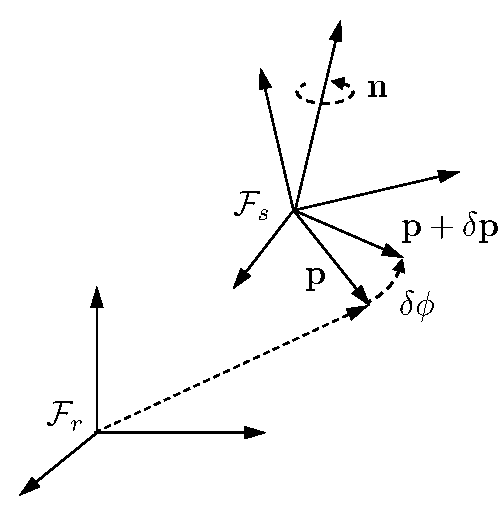
\includegraphics[width=\linewidth]{chap2_preliminaries/figures/coriolis_formula}\\
  \caption{Derivation of the equation of Coriolis.}
  \label{fig:coriolis_formula}
\end{marginfigure}
On the other hand, assume that $\mathbf{p}$ is fixed in
$\mathcal{F}_s$ but that $\mathcal{F}_s$ is rotating with respect to
$\mathcal{F}_r$, and let $\omegabf_{s/r}$ be the instantaneous axis of
rotation and $\delta\phi$ the (right-handed) rotation angle.  Then
the Rodrigues formula~\eqref{eq:rodrigues_1} gives
\begin{align*}
\mathbf{p}+\delta\mathbf{p} 
	&=\Big[I + \sin(\delta\phi)\ss{\nbf} + (1-\cos(\delta\phi))\ss{\nbf}^2\Big]\pbf \\
	&\approx \Big[I + \delta\phi \ss{\nbf} + (\delta\phi^2)\ss{\nbf}^2\Big]\pbf \\
	&\approx \Big[I + \delta\phi \ss{\nbf}\Big]\pbf \\
	&= \pbf + (\delta\phi\nbf)\times \pbf,
\end{align*}
which implies, after dividing both sides by $\delta t$ that
\[
\frac{\delta\mathbf{p}}{\delta t} \approx \frac{\delta\phi}{\delta
t}\nbf \times \mathbf{p}.
\]
Taking the limit as $\delta t \to 0$ and defining the angular
velocity of $\mathcal{F}_s$ with respect to $\mathcal{F}_r$ as
$\boldsymbol{\omega}_{s/r}
\defeq \dot{\phi}\nbf$ we get
\begin{equation}\label{eq:coriolis2}
\frac{d\mathbf{p}}{dt_r} = \omegabf_{s/r}\times\mathbf{p}.
\end{equation}
Since differentiation is a linear operator we can combine
Equations~\eqref{eq:coriolis1}
and~\eqref{eq:coriolis2} to obtain
\begin{equation}\label{eq:coriolis}
\frac{d\mathbf{p}}{dt_r} = \frac{d\mathbf{p}}{dt_s} + \boldsymbol{\omega}_{s/r}
\times\mathbf{p},
\end{equation}
which is the equation of Coriolis.

Note that the vectors in Equation~\eqref{eq:coriolis} have not yet been expressed with respect to a particular coordinate system.  In fact, we can express each vector in Equation~\eqref{eq:coriolis} with respect to any given coordinate frame.  However, care needs to be taken to express the vectors {\bf after} the differentiation operator. For example, expressing the equations in frame $\cal{F}_s$ we have 
\[
\left(\frac{d\mathbf{p}}{dt_r}\right)^s = \left(\frac{d\mathbf{p}}{dt_s}\right)^s + \omegabf_{s/r}^s \times \mathbf{p}^s.
\]
Note however that $\left(\frac{d\mathbf{p}}{dt_r}\right)^s$ is not necessarily equal to $\frac{d\left(\mathbf{p}^s\right)}{dt_r}$.  For example, suppose that $\ibf_s$ is the unit vector along the $x$-axis of the $s$-frame that is undergoing a pure rotation denoted by $\boldsymbol{\omega}_{s/r}$.  Then it is clear that $\left(\frac{d\ibf_s}{dt_r}\right)^s = \omegabf_{s/r}^s\times\ibf_s^s \neq 0$.  However, since $\ibf_s^s = (1, 0, 0)^\top$ is constant in the $s$-frame, $\frac{d\left(\ibf_s^s\right)}{dt_r}=0$.  
%
It is true however that $\left(\frac{d\mathbf{p}}{dt_s}\right)^s =  \frac{d\left(\mathbf{p}^s\right)}{dt_s}$. In general, if the time derivative of the vector is with respect to the same frame in which the vector is being expressed, then the derivative of the vector with respect to frame $s$ expressed in frame $s$ is equal to the derivative of the vector expressed in frame $s$ with respect to frame $s$. 


We also note that the derivative of a scalar is independent of the coordinate frame with which the derivative is being taken.  In this book we will use the dot-notation to mean differentiation with respect to time, only when the derivative is applied component wise, and each component is being differentiated as a scalar.  In that sense, if $\mathbf{p}^s = (x, y, z)^{\top}$, then 
\[
\frac{d\mathbf{p}^s}{dt_s} = \begin{pmatrix} \dot{x} \\ \dot{y} \\ \dot{z} \end{pmatrix}.
\]
When vectors are expressed relative to a coordinate frame, then Equation~\eqref{eq:coriolis} can be written as
\[
\left(\frac{d\mathbf{p}}{dt_r}\right)^q = \left(\frac{d\mathbf{p}}{dt_s}\right)^q+ \ss{\omegabf_{s/r}^q}\mathbf{p}^q.
\]

%%+++++++++++++++++++
\subsection{Rotational Kinematics} 

The Coriolis equation~\eqref{eq:coriolis}
facilitates the derivation of the rotational kinematics of a rigid body.  Defining coordinate frame $s$ as $\mathcal{F}_s = \{\ibf_s, \jbf_s, \kbf_s\}$,
and suppose that frame $s$ is rotated relative to frame $r$ by angular velocity $\omegabf_{s/r}$, then the Coriolis formula gives
\[
\frac{d\ibf_s}{dt_r} = \frac{d\ibf_s}{dt_s} + \omegabf_{s/r}\times\ibf_s, \qquad 
\frac{d\jbf_s}{dt_r} = \frac{d\jbf_s}{dt_s} + \omegabf_{s/r}\times\jbf_s, \qquad 
\frac{d\kbf_s}{dt_r} = \frac{d\kbf_s}{dt_s} + \omegabf_{s/r}\times\kbf_s.
\]
Since the coordinate axes are stationary in their own frame, $\frac{d\ibf_s}{dt_s}=\frac{d\jbf_s}{dt_s}=\frac{d\kbf_s}{dt_s}=0$, and we have
\[
\frac{d\ibf_s}{dt_r} = \omegabf_{s/r}\times\ibf_s, \qquad 
\frac{d\jbf_s}{dt_r} = \omegabf_{s/r}\times\jbf_s, \qquad 
\frac{d\kbf_s}{dt_r} = \omegabf_{s/r}\times\kbf_s.
\]
Expressing all vectors in frame $r$ and rewriting in matrix notation gives
\begin{align*}
\begin{bmatrix} \frac{d\ibf_s^r}{dt_r} & \frac{d\jbf_s^r}{dt_r} & \frac{d\kbf_s^r}{dt_r} \end{bmatrix} 
&= \begin{bmatrix} \ss{\omegabf_{s/r}^r}\ibf_s^r, & \ss{\omegabf_{s/r}^r}\jbf_s^r, & \ss{\omegabf_{s/r}^r}\kbf_s^r, \end{bmatrix}  \\
&= \ss{\omegabf_{s/r}^r} \begin{bmatrix} \ibf_s^r & \jbf_s^r & \kbf_s^r \end{bmatrix}  \\
&= \ss{\omegabf_{s/r}^r} R_s^r. 
\end{align*}
Defining 
\[
\dot{R}_s^r \defeq \begin{bmatrix} \frac{d\ibf_s^r}{dt_r} & \frac{d\jbf_s^r}{dt_r} & \frac{d\kbf_s^r}{dt_r} \end{bmatrix}
\]
gives the rotational kinematics as
\begin{equation}\label{eq:rotational_kinematics_1}
\dot{R}_s^r = \ss{\omegabf_{s/r}^r} R_s^r.
\end{equation}

Suppose that we equate the $s$-frame with the body frame $\mathcal{F}_b$ and the $r$-frame with the inertial frame $\mathcal{F}_i$, then Equation~\eqref{eq:rotational_kinematics_1} becomes
\[
\dot{R}_b^i = \ss{\omegabf_{b/i}^i} R_b^i,
\]
which is given in terms of the angular velocity $\omegabf_{b/i}$ expressed in the inertial frame.  However, the angular velocity can be measured with respect to the body frame using rate gyros.  Therefore, it is preferable to write the rotational kinematics in terms of $\omegabf_{b/i}^b$.  Noting that $\omegabf_{s/r}^r = R_s^r \omegabf_{s/r}^s$, we get
\marginnote{Note that we have used Equation~\eqref{eq:skew_matrix_6} $\ss{(R\abf)}=R\ss{\abf}R^\top$.}
\begin{align*}
\dot{R}_s^r &= \ss{\omegabf_{s/r}^r} R_s^r	\\
			&= \ss{R_s^r\omegabf_{s/r}^s} R_s^r \\
			&= R_s^r \ss{\omegabf_{s/r}^s} (R_s^r)^\top R_s^r \\
			&= R_s^r \ss{\omegabf_{s/r}^s}.
\end{align*}
We have therefore established the relationship for rotational kinematics as
\begin{align}
	\dot{R}_s^r &= R_s^r \ss{\omegabf_{s/r}^s} \label{eq:rotational_kinematics} \\
				&= \ss{\omegabf_{s/r}^r} R_s^r \label{eq:rotational_kinematics_alt}
\end{align}

Applying these formulas to the body and inertial frames we have
\begin{align}
\dot{R}_b^i &= R_b^i \ss{\omegabf_{b/i}^b} = \ss{\omegabf_{b/i}^i} R_b^i \label{eq:rotational_kinematics_b_i} \\
\dot{R}_i^b &= -\ss{\omegabf_{b/i}^b} R_i^b = - R_i^b \ss{\omega_{b/i}^i}.\label{eq:rotational_kinematics_i_b}
\end{align}
Applying these formulas to the gimbal and body frames we have
\begin{align*}
\dot{R}_g^b &= R_g^b \ss{\omegabf_{g/b}^g} = \ss{\omegabf_{g/b}^b} R_g^b \\
\dot{R}_b^g &= -\ss{\omegabf_{g/b}^g} R_b^g = - R_b^g \ss{\omega_{g/b}^b}.
\end{align*}

Using the conclusions of the previous section, we can get the following result.
\begin{lemma}
If $\mathbf{p}$ is a vector and $\mathcal{F}^s$ and $\mathcal{F}^r$ are coordinate frames, with $R_r^s\in SO(3)$ being the rotation between frames, then
\[
\left(\frac{d\mathbf{p}}{dt_r}\right)^s = R_r^s\frac{d (\mathbf{p}^r)}{dt_s}.
\]	
\end{lemma}
\begin{proof}
	\begin{align*}
			\left(\frac{d\mathbf{p}}{dt_r}\right)^s 
				&= \left(\frac{d\mathbf{p}}{dt_s}\right)^s + \omegabf_{s/r}^s \times \mathbf{p}^s \\
				&= \frac{d(\mathbf{p}^s)}{dt_s} + \ss{\omegabf_{s/r}^s} R_r^s \mathbf{p}^r \\
				&= \frac{d(R_r^s\mathbf{p}^r)}{dt_s} + \ss{\omegabf_{s/r}^s} R_r^s \mathbf{p}^r \\
				&= \frac{dR_r^s}{dt_s}\mathbf{p}^r + R_r^s \frac{d(\mathbf{p}^r)}{dt_s} +\ss{\omegabf_{s/r}^s} R_r^s \mathbf{p}^r \\
				&= -\ss{\omegabf_{s/r}^s} R_r^s\mathbf{p}^r + R_r^s \frac{d(\mathbf{p}^r)}{dt_s} +\ss{\omegabf_{s/r}^s} R_r^s \mathbf{p}^r \\
				&= R_r^s \frac{d(\mathbf{p}^r)}{dt_s}.
	\end{align*}
\end{proof}




%%+++++++++++++++++++
\subsection{Integrating the Rotational Kinematics}
In robotics and flying vehicle applications, we often need to integrate the rotational kinematics given samples of the rate gyros. 
In this section we describe numerical approximations to the equation
\begin{equation}\label{eq:Rdot-integrating-1}
\dot{R}=R\ss{\omegabf},
\end{equation}
assuming that $\omegabf$ is either piecewise constant, or piecewise linear between samples.  Since $R$ evolves on the set $SO(3)$, the simple Euler integration scheme $R[k]=R[k-1]+TR[k-1]\ss{\omegabf[k]}$ is particularly bad since $R$ immediately leaves $SO(3)$.  A common strategy is to re-orthonormalize $R$ after every integration step, but this is an ad~hoc scheme that may introduce additional drift in the integration process.  If $\omegabf$ is assumed to be piecewise constant or piecewise linear between samples, then the kinematics can be integrated exactly.  

We begin by solving the differential equation~\eqref{eq:Rdot-integrating-1}.
\begin{lemma} \label{eq:rotation_kinematics_solution}
The solution to Equation	~\eqref{eq:Rdot-integrating-1} with initial condition $R(t_0) = R_0$ is given by
\begin{equation}\label{eq:rotation_kinematics_solution}
R(t) = R(t_0)\exp\left(\ss{\int_{t_0}^t \omegabf(\tau) d\tau }\right).
\end{equation}
\end{lemma}
\begin{proof}
Rewrite Equation~\eqref{eq:Rdot-integrating-1} as
\[
\dot{R} - R\ss{\omegabf} = 0,
\]
and multiply on the left by the integrating factor $\exp\left(-\ss{\int_{t_0}^t\omegabf(\tau)d\tau}\right)$ to get
\begin{align*}
\left(\dot{R} - R\ss{\omegabf}\right)\exp\left(-\ss{\int_{t_0}^t \omegabf(\tau)d\tau}\right) &=\\
\frac{d}{dt}\left[R\exp\left(-\ss{\int_{t_0}^t \omegabf(\tau)d\tau}\right)\right] &= 0.
\end{align*}
Integrating both sides and applying the fundamental theorem of Calculus gives 
\marginnote{The fundamental theorem of Calculus states that $\int_a^b dF = F(b)-F(a)$.}
\begin{equation}\label{eq:rotation_kinematics_solution}
R(t)\exp\left(\ss{-\int_{t_0}^t \omegabf(\tau) d\tau} \right) - R(t_0)\exp\left(\ss{-\int_{t_0}^{t_0} \omegabf(\tau) d\tau} \right) = 0.
\end{equation}
\marginnote{In deriving this expression, we have used the fact that $\exp(-Mt)=(\exp(Mt))^{-1}$ and $\exp(Mt)\exp(-Mt_0)=\exp(M(t-t_0))$.}
Multiplying on the left by $\exp\left(\ss{\int_{t_0}^t \omegabf(\tau) d\tau }\right)$ gives the result.
\end{proof}

In the following, we let $T_s$ represent the sample rate, and we will use the notation $R[k]=R(kT_s)$ and $\omegabf[k]\defeq\omegabf(kT_s)$.  We say that $\omegabf$ is piecewise constant between samples if
\[
\omegabf(t) = \omegabf[k]
\]
for $(k-1)T_s < t \leq kT_s$, and we say that $\omegabf$ is piecewise linear between samples if
When $\omegabf$ is piecewise linear between samples, i.e., when
\[
 \omegabf(t) = \left(\frac{kT_s-t}{T_s}\right)\omegabf[k-1] + \left(\frac{(t-(k-1)T_s)}{T_s}\right)\omegabf[k]
\]
for $(k-1)T_s \leq t < kT_s$.
\begin{lemma}
 If the angular velocity is piecewise constant between samples, then from Equation~\eqref{eq:rotation_kinematics_solution} we get
\begin{equation}\label{eq:rotational_int_constant_omega}
R[k] = R[k-1] \exp\left(T_s \ss{\omegabf[k]} \right).
\end{equation}
Similarly, if the angular velocity is piecewise linear between samples, then 
\begin{equation}\label{eq:rotational_int_linear_omega}
R[k] = R[k-1] \exp\left(\frac{T_s}{2} \ss{\omegabf[k]+\omegabf[k-1]}\right).
\end{equation}
\end{lemma}
\begin{proof}
If the sample rate is $T_s$, then letting $t=kT_s$ and $t_0=(k-1)T_s$, and using the notation $R[k]=R(kT)$, we get
\[
R[k] = R[k-1] \exp\left(\ss{\int_{(k-1)T_s}^{kT_s} \omegabf(\tau) d\tau }\right).
\]
When $\omegabf$ is piecewise constant between samples we have
\[
\int_{(k-1)T_s}^{kT_s} \omegabf(\tau) d\tau = \omegabf[k]T_s,
\]
resulting in Equation~\eqref{eq:rotational_int_constant_omega}.
When $\omegabf$ is piecewise linear between samples we get 
\begin{align*}
\int_{(k-1)T_s}^{kT_s} \omegabf(\tau) d\tau
	&= \int_{(k-1)T_s}^{kT_s} \left[\left(\frac{kT_s-\tau}{T_s}\right)\omegabf[k-1] + \left(\frac{\tau-(k-1)T_s}{T_s}\right)\omegabf[k]\right] d\tau \\
	&= \frac{T_s}{2} \left(\omegabf[k]+\omegabf[k-1]\right),
\end{align*}
resulting in Equation~\eqref{eq:rotational_int_linear_omega}.
\end{proof}

%%+++++++++++++++++++
\subsection{Numerical Differentiation of the Rotation Matrix}
\label{sec:numerical_differentiation_of_R}
Similarly, if we are given samples of $R(t)$ at sample rate $T_s$, we would like to approximate the angular velocity $\omegabf(t)$.   
\begin{lemma}
Given the rotational kinematics in Equation~\eqref{eq:Rdot-integrating-1}, and measured rotation matrices $R[k]$ and $R[k-1]$, then
\begin{equation}\label{eq:rotational_diff}
\omegabf[k]\approx \left[\frac{1}{T_s}\log\left(R^\top[k-1]R[k]\right)\right]^{\vee}.
\end{equation}
\end{lemma}
\begin{proof}
From Equation~\eqref{eq:rotational_int_constant_omega} we have
\[
R[k] = R[k-1]\exp\left(T_s\ss{\omegabf[k]}\right).
\]
Solving for $\ss{\omegabf[k]}$ gives
\[
\ss{\omegabf[k]} = \frac{1}{T_s}\log\left(R^\top[k-1]R[k]\right)
\]
from which we obtain Equation~\eqref{eq:rotational_diff}.
\end{proof}



%++++++++++++++++++++++++++++++++++++++++++++++++++++++++++++++++
\subsection{Quaternion Kinematics}
\rwbcomment{Add this later.}

%++++++++++++++++++++++++++++++++++++++++++++++++++++++++++++++++
\subsection{Euler Angle Kinematics}
\rwbcomment{Add this later.}

%++++++++++++++++++++++++++++++++++++++++++++++++++++++++++++++++
\subsection{Rotation Vector Kinematics}
\rwbcomment{Add this later.}

%-----------------------------------------------------------
\section{Homogeneous Transformations}
\label{sec:homogeneous transformations}

In this section we discuss the use of homogeneous transformations to represent rigid body motion that includes both translation and rotation simultaneously.  We will show that $4\times 4$ matrices can be used to represent rigid body motion.
%
\begin{marginfigure}[-2in]
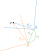
\includegraphics[width=\linewidth]{chap2_preliminaries/figures/transform_passive}
\caption{Illustration of a passive transformation}
\label{fig:passive_transform}
\end{marginfigure}
Considering Figure~\ref{fig:passive_transform}, 
suppose that a robot moves from a pose represented by frame $\mathcal{F}_a$ to a pose represented by frame $\mathcal{F}_b$.  If the robot measures the position of point $\pbf$ in frame $a$ and from odometry knows its relative motion represented by the rotation matrix $R_a^b$ and the translation vector $\tbf_{a/b}^b$, then the position of $\pbf$ relative to frame $\mathcal{F}_b$ is given by
\begin{equation}\label{eq:homogenenous_1}
\rbf_{p/b}^b = R_a^b \rbf_{p/a}^a + \tbf_{a/b}^b.
\end{equation}
We would like to represent this relative motion using a matrix.  
%
To do so, we introduce the use of {\em homogeneous coordinates} for position.  The homogeneous coordinates of the vector $\pbf^c$ expressed in a general frame $\mathcal{F}_c$ are given by
\[
\bar{\pbf}^c \defeq \begin{pmatrix} \pbf^c \\ 1 \end{pmatrix},
\]
where $1$ has been appended as the last coordinate.  
%
Using this notation, Equation~\eqref{eq:homogenenous_1} can be written as
\[
\bar{\rbf}_{p/b}^b = \begin{pmatrix} \rbf_{p/b}^b \\ 1 \end{pmatrix} = \begin{pmatrix} R_a^b & \tbf_{a/b}^b \\ 0 & 1 \end{pmatrix}\begin{pmatrix} \rbf_{p/a}^a \\ 1 \end{pmatrix} = T_a^b \bar{\rbf}_{p/a}^a,
\]
where
\[
T_a^b \defeq \begin{pmatrix} R_a^b & \tbf_{a/b}^b \\ 0 & 1 \end{pmatrix}
\]
is called a homogeneous transformation matrix.
%
It is important to note is that the translation
vector is defined in the \emph{destination} frame, rather than the
origin frame of the rotation matrix. 

%
%
%
%
%Now we venture into the world of rigid body transformations. These
%allow us to represent both translation and rotation simultaneously.
%As with rotations, there are two popular representations that I will
%consider in this document, the first is matrix-based, the set of $4\times4$
%matrices, commonly known as $SE(3)$. The second (like
%rotations) will be based on complex numbers, dual unit quaternions.
%There are actually other representations, but we will see later all
%of these groups share the same Lie Algebra! Therefore, we can choose
%the representation that we feel most comfortable with, or is the most
%efficient, etc... It really doesn't matter, which is a great thing.

\subsection{Homogeneous Transformation Matrices}

Define the set
\[
SE(3) = \left\{T\in\mathbb{R}^{4\times 4} ~|~ T=\begin{pmatrix} R & \tbf \\ 0 & 1\end{pmatrix}, R\in SO(3), \tbf\in\mathbb{R}^3 \right\},
\]
which is called the {\em Special Euclidean group of dimension 3}.  We can derive the following facts about elements of $SE(3)$.

\begin{lemma}[Closed under Multiplication]
If $T_1, T_2\in SE(3)$, then $T_3=T_2 T_1 \in SE(3)$.
\end{lemma}
\begin{proof}
	\begin{align*}
	T_3 &= \begin{pmatrix} R_2 & \tbf_2 \\ 0 & 1 \end{pmatrix} \begin{pmatrix} R_1 & \tbf_1 \\ 0 & 1 \end{pmatrix} \\
	    &= \begin{pmatrix} R_2 R_1 & R_2\tbf_1 + \tbf_2 \\ 0 & 1 \end{pmatrix},
	\end{align*}
	which is an element of $SE(3)$ since $SO(3)$ is closed under multiplication and $R_2\tbf_1 + \tbf_2\in\mathbb{R}^3$.
\end{proof}

\begin{lemma}[Inverse]
If 
\[
T=\begin{pmatrix} R & \tbf \\ 0 & 1\end{pmatrix} \in SE(3),
\]	
then 
\[
T^{-1} =\begin{pmatrix} R^\top & -R^\top\tbf \\ 0 & 1\end{pmatrix} \in SE(3).
\]
\end{lemma}
\begin{proof}
The fact that $TT^{-1} = T^{-1}T = I$ can be shown by direct calculation.  Since $R^\top\in S(3)$ when $R\in SO(3)$ and $-R^\top\tbf\in\mathbb{R}^3$ it follows that $T^{-1}\in SE(3)$.
\end{proof}

\begin{lemma} [Determinant]
If $T\in SE(3)$, then $\det(T)=1$.
\end{lemma}
\begin{proof}
Follows from $\det{T}=\det(R)\det(1)=1$.
\end{proof}
\begin{lemma} [Concatination]
If $T_a^b\in SE(3)$ and $T_b^c\in SE(3)$ are homogeneous transformations from frames $a$ to $b$ and $b$ to $c$, respectively, then the homogeneous transformation from frame $a$ to frame $c$ is given by
\begin{align*}
T_{a}^{c} & =T_{b}^{c}\cdot T_{a}^{b}\\
 & =\begin{pmatrix}R_{b}^{c} & \tbf_{c/b}^{c}\\
0 & 1
\end{pmatrix}\cdot\begin{pmatrix}R_{a}^{b} & \tbf_{b/a}^{b}\\
0 & 1
\end{pmatrix}\\
 & =\begin{pmatrix}R_{b}^{c}R_{a}^{b} & R_{b}^{c}\tbf_{b/a}^{b}+\tbf_{c/b}^{c}\\
0 & 1
\end{pmatrix}.
\end{align*}
\end{lemma}

%----------------------------------------
\subsection{Passive and Active Transformations}

The same notion of passive and active transformations discussed with
rotations applies here. To perform a passive transformation with $SE(3)$,
we just pad the vector to be rotated with an extra $1$ at the bottom,
and multiply by the homogeneous transformation matrix. 

\begin{marginfigure}
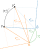
\includegraphics[width=\linewidth]{chap2_preliminaries/figures/transform_active}
\caption{Illustration of an active transformation.}
\label{fig:active_transform}
\end{marginfigure}

An active transformation occurs by multiplying by the inverse of the
passive transform as shown in Figure~\ref{fig:passive_transform}.
Just as with rotations, If you walk through the coordinate frames
of an active transformation, you'll see that the coordinate frames
don't line up right in our notation. This is because the active transformation
does not preserve the location. Instead we have defined a new location,
based on the coordinates of $p$ in frame $a$ projected into frame
$b$. This is represented by the $p^{\star}$ notation
in Figure~\ref{fig:active_transform}.

%Transform matrices are an obvious extension of rotation matrices.
%However, just like rotation matrices, the complex number representation
%is more efficient. This brings us to our next transform parameterization:
%dual unit quaternions.

%++++++++++++++++++++++++++++++++++++++++++++++++++++++++++++++
\subsection{Rigid body kinematics}
As we saw in Section~\ref{sec:rotational_kinematics}, the rotational kinematics are given by
\begin{equation}\label{eq:rotational_dynamics_kinematics}
\dot{R}_s^r = R_s^r \ss{\omegabf_{s/r}^s}.
\end{equation}
In this section we will derive a similar expression for homogeneous transformation matrices.  
Let
\[
T_s^r = \begin{pmatrix} R_s^r & \tbf_{s/r}^r \\ 0 & 1 \end{pmatrix},
\]
and differentiate to get
\begin{align*}
\dot{T}_s^r &= \begin{pmatrix} \dot{R}_s^r & \dot{\tbf}_{s/r}^r \\ 0 & 0 \end{pmatrix} \\
&= \begin{pmatrix} R_s^r\ss{\omegabf_{s/r}^s} & R_s^r\dot{\tbf}_{s/r}^s \\ 0 & 0 \end{pmatrix} \\
&= \begin{pmatrix} R_s^r & \tbf_{s/r}^r \\ 0 & 1 \end{pmatrix} \begin{pmatrix} \ss{\omegabf_{s/r}^s} & \dot{\tbf}_{s/r}^s \\ 0 & 0 \end{pmatrix}
\end{align*}
Define the relative velocity as
\[
\vbf_{s/r} \defeq \dot{\tbf}_{s/r},
\]
and the relative twist as
\[
\nubf_{s/r} = \begin{pmatrix} \vbf_{s/r} \\ \omegabf_{s/r} \end{pmatrix} \in \mathbb{R}^6.
\]
We also define the ``wedge'' operator for twist as 
\[
\begin{pmatrix} \vbf_{s/r} \\ \omegabf_{s/r} \end{pmatrix}^\wedge \defeq \begin{pmatrix} \ss{\omegabf_{s/r}} & \vbf_{s/r} \\ 0 & 0 \end{pmatrix},
\]
and we define $\se(3)$ to be the set of all ``wedged'' twist vectors:
\[
\se(3) = \left\{ \Omega = \begin{pmatrix}\ss{\omegabf} & \nubf \\ 0 & 0\end{pmatrix} ~|~ \nubf, \omegabf \in \mathbb{R}^3 \right\}.
\] 

We have that the homogeneous transformation matrix evolves as
\begin{equation}\label{eq:homogeneous_diffeq}
\dot{T}_s^r = T_s^r (\nubf_{s/r}^s)^\wedge,
\end{equation}
where $T_s^r\in SO(3)$ and $(\nubf_{s/r}^s)^\wedge\in\se(3)$, 
which has the same form as Equation~\eqref{eq:rotational_dynamics_kinematics}.  Analogous to Equations~\eqref{eq:rotational_kinematics_b_i} and~\eqref{eq:rotational_kinematics_i_b}, the kinematics of the multirotor body frame relative to the inertial frame are given by
\begin{align}
\dot{T}_b^i &= T_b^i (\nubf_{b/i}^b)^\wedge = (\nubf_{b/i}^i)^\wedge T_b^i \label{eq:homogeneous_kinematics_b_i} \\
\dot{T}_i^b &= -(\nubf_{b/i}^b)^\wedge T_i^b = - T_i^b (\nubf_{b/i}^i)^\wedge.\label{eq:homogeneous_kinematics_i_b}
\end{align}

The following lemma provide a solution to the differential equation~\eqref{eq:homogeneous_diffeq}.
\begin{lemma}
The solution to differential matrix equation
\[
\dot{T} = T\nubf^\wedge
\]
with initial condition $T(t_0)$ is given by
\begin{equation}\label{eq:homogeneous_kinematics_solution}
T(t) = T(t_0)\exp\left(\int_{t_0}^t \nubf(\tau)^\wedge d\tau \right).
\end{equation}
\end{lemma}
\begin{proof}
Similar to Lemma~\ref{eq:rotation_kinematics_solution}.	
\end{proof}

We now derive an expression for the exponential of a matrix $\Omega\in\se(3)$.
\begin{lemma}
If $\nubf^\wedge = \begin{pmatrix} \ss{\omegabf} & \vbf \\ 0 & 0 \end{pmatrix} \in \se(3)$, then
\[
\exp(\nubf^\wedge) = \begin{pmatrix} \exp(\ss{\omegabf}) & W(\ss{\omegabf})\vbf \\ 0 & 1 \end{pmatrix},
\]
where
\[
W(\ss{\omegabf}) \defeq I+\left(\frac{1-\cos\left(\norm{\omegabf}\right)}{\norm{\omegabf}^{2}}\right)\ss{\omegabf}+\left(\frac{\norm{\omegabf}-\sin\left(\norm{\omegabf}\right)}{\norm{\omegabf}^{3}}\right)(\ss{\omegabf})^{2}.
\]
Furthermore $\exp(\nubf^\wedge) \in SE(3)$.
\end{lemma}
\begin{proof}
\begin{align*}
\exp\begin{pmatrix}\ss{\omegabf} & \vbf\\
0 & 0
\end{pmatrix} & =I+\begin{pmatrix}\ss{\omegabf} & \vbf\\
0 & 0
\end{pmatrix}+\frac{1}{2!}\begin{pmatrix}\ss{\omegabf} & \vbf\\
0 & 0
\end{pmatrix}^{2}+\frac{1}{3!}\begin{pmatrix}\ss{\omegabf} & \vbf\\
0 & 0
\end{pmatrix}^{3}+\cdots\\
 & =I+\begin{pmatrix}\ss{\omegabf} & \vbf\\
0 & 0
\end{pmatrix}+\frac{1}{2!}\begin{pmatrix}(\ss{\omegabf})^{2} & \ss{\omegabf}\vbf\\
0 & 0
\end{pmatrix}+\frac{1}{3!}\begin{pmatrix}(\ss{\omegabf})^{3} & (\ss{\omegabf})^{2}\vbf\\
0 & 0
\end{pmatrix}+\cdots\\
 & =\begin{pmatrix}\exp\left(\ss{\omegabf}\right) & W(\ss{\omegabf}) \vbf\\
0 & 0
\end{pmatrix},
\end{align*}
where
\begin{align*}
W(\ss{\omegabf}) &= I+\frac{1}{2}\ss{\omegabf}+\frac{1}{3!}(\ss{\omegabf})^{2} + \ddots \\
	&= I + \sum_{k=0}^{\infty}\left(\frac{(\ss{\omegabf})^{\left(2k+1\right)}}{\left(2k+2\right)!}+\frac{(\ss{\omegabf})^{\left(2k+2\right)}}{\left(2k+3\right)!}\right).
\end{align*}
Recall from the proof of Lemma~\ref{lem:rodrigues_exponential} that 
\begin{align*}	
\ss{\nbf}^{(2m+1)} &= (-1)^m\ss{\nbf} \\
\ss{\nbf}^{(2m+2)} &= (-1)^m\ss{\nbf}^2,
\end{align*}
from which we get
\begin{align*}
W(\ss{\omegabf}) 
 & =I+\sum_{k=0}^{\infty}\left(\frac{\left(-1\right)^{k}\norm{\omegabf}^{2k}}{\left(2k+2\right)!}\right)\ss{\omegabf}+\sum_{k=0}^{\infty}\left(\frac{\left(-1\right)^{k}\norm{\omegabf}^{2k}}{\left(2k+3\right)!}\right)(\ss{\omegabf})^{2}\\
 & =I+\left(\frac{1}{2}-\frac{\norm{\omegabf}^{2}}{4!}+\frac{\norm{\omegabf}^{4}}{6!}+\cdots\right)\ss{\omegabf}+\left(\frac{1}{3!}-\frac{\norm{\omegabf}^{2}}{5!}+\frac{\norm{\omegabf}^{4}}{7!}+\cdots\right)(\ss{\omegabf})^{2}\\
 & =I+\left(\frac{1-\cos\left(\norm{\omegabf}\right)}{\norm{\omegabf}^{2}}\right)\ss{\omegabf}+\left(\frac{\norm{\omegabf}-\sin\left(\norm{\omegabf}\right)}{\norm{\omegabf}^{3}}\right)(\ss{\omegabf})^{2}.
\end{align*}
The fact that $\exp(\Omega)\in SE(3)$ follows from the definition of $SE(3)$ since $\exp(\ss{\omegabf})\in SO(3)$ and $W(\ss{\omegabf})\vbf\in\mathbb{R}^3.$
\end{proof}
Note that 
\begin{align*}
	\lim_{x\to 0}\frac{1-cos(x)}{x^2} &= \lim_{x\to 0}\frac{ 1-(1-\frac{x^2}{2!}+\frac{x^4}{4!}-\cdots}{x^2} 
        							  = \lim_{x\to 0} \frac{1}{2!}-\frac{x^2}{4!}+\cdots = \frac{1}{2} \\
   	\lim_{x\to 0}\frac{x-\sin(x)}{x^3} &= \lim_{x\to 0}\frac{x-(x-\frac{x^3}{3!}+\frac{x^5}{5!}-\cdots}{x^3}
   	                                    = \lim_{x\to 0} \frac{1}{3!} - \frac{x^2}{5!} + \cdots = \frac{1}{6},
\end{align*}
and therefore $W(\ss{\omegabf})$ is well defined as $\omegabf\to 0$.

The logarithm also has a closed form.
\begin{lemma}
If $R\in SO(3)$ and $\tbf\in\mathbb{R}^3$, then
\[
\log\begin{pmatrix} R & \tbf \\ 0 & 1 \end{pmatrix} = \begin{pmatrix}\log(R) & W^{-1}(R)\tbf \\ 0 & 0 \end{pmatrix},
\]
where
\[
W^{-1}(R) = I - \frac{1}{2}\ss{\omegabf} + \frac{1}{\norm{\omegabf}^2}\left(1-\frac{\norm{\omegabf}\sin(\norm{\omegabf})}{2(1-\cos(\norm{\omegabf}))}\right)\ss{\omegabf}^2,
\]
where $\omegabf = \log(R)^\vee$.
\end{lemma}
\begin{proof}
From the previous lemma we know that
\[
\log\begin{pmatrix} \exp(\ss{\omegabf}) & W\vbf \\ 0 & 1 \end{pmatrix} 
= \begin{pmatrix} \ss{\omegabf} & \vbf \\ 0 & 0 \end{pmatrix}.
\]
Equation $R=\exp(\ss{\nubf^\wedge})$ and $\tbf = W\vbf$ shows that $\omegabf=\log(R)^\vee$ and $\vbf=W^{-1}\tbf$.
\end{proof}
After multiple uses of L'Hopital's rule, it can be shown that 
\[
\lim_{\theta\to 0} \frac{1}{\theta^2}\left(1 - \frac{\theta\sin\theta}{2(1-\cos\theta)}\right) = \frac{1}{12},
\]
which implies that $W^{-1}(R)$ is well defined as $R\to I$ (i.e., $\omegabf\to 0$).


%%++++++++++++++++++++++++++++++++++++++++++++++++++++++++++++++++
%\subsection{Body-Centric vs Inertial Representation}
%
%In robotics or computer vision, we are typically concerned with rotations
%so that we can describe the movement of physical objects. When we
%do this, it turns out that choice of coordinate frame also introduces
%some interesting consequences that may or may not be intentional.
%Rotational dynamics of any arbitrary coordinate frame $j$ with respect
%to another coordinate frame $i$ is given by
%
%\[
%\dot{R}_{i}^{j}=R_{i}^{j}\ss{(\omegabf_{i/j}^{i})}.
%\]
%However, let's study a concrete example: the dynamics of some rigid
%body undergoing pure rotation. If we define some inertial frame $I$
%and the moving, body frame as $b$, then the dynamics of the \emph{body-centric}
%rotation matrix (i.e. body$\to$inertial), we get 
%
%\begin{equation}
%\dot{R}_{b}^{I}=R_{b}^{I}\ss{(\omegabf_{b/I}^{b})},\label{eq:body_rot_dyn}
%\end{equation}
%and the \emph{inertial} rotation matrix is (inertial$\to$body) evolves
%according to
%
%\begin{equation}
%\dot{R}_{I}^{b}=R_{I}^{b}\ss{(\omegabf_{I/b}^{I})}.\label{eq:inertial_rotation_dynamics}
%\end{equation}
%This is all fine, except that we typically measure angular velocity
%in the body coordinate frame $\omegabf_{b/I}^{b}.$ Therefore, it is much
%more convenient to express Eq. \ref{eq:inertial_rotation_dynamics}
%in terms of body angular rates. If we do this, then we get
%
%\begin{align*}
%\dot{R}_{I}^{b} & =R_{I}^{b}\ss{(-R_{b}^{I}\omegabf_{b/I}^{b})} & \text{(Negate and rotate $\omegabf$)}\\
% & =-\ss{(\omegabf_{b/I}^{b})}R_{I}^{b}, & \text{(Eq. \ref{eq:skew_trick_2})}
%\end{align*}
%which can also be easily derived as the transpose of Eq \ref{eq:body_rot_dyn}.
%The desire to express our angular rates in terms of the body frame
%induces a similar effect in unit quaternion dynamics, except that
%it is reversed due to the reversed order of concatenation:
%
%\begin{align}
%\dot{\qbf}_{I}^{b} & =\frac{1}{2}\qbf_{I}^{b}\cdot\begin{pmatrix}0\\
%\omegabf_{b/I}^{b}
%\end{pmatrix}\label{eq:quaternion_dynamics}\\
%\dot{\qbf}_{b}^{I} & =-\frac{1}{2}\begin{pmatrix}0\\
%\omegabf_{b/I}^{b}
%\end{pmatrix}\cdot\qbf_{b}^{I}.\nonumber 
%\end{align}
%
%Any advantage to expressing attitude in body-centric vs. inertial
%coordinates will be use-case specific, so both representations are
%used widely in literature. Because both representations are often
%used, however, it can sometimes be confusing to compare two works
%which may be expressing their attitude differently, especially if
%neither work is specific about their representation.


%\subsection{The Solution to the Rotational Dynamics Equation}
%
%Equations \ref{eq:body_rot_dyn} and \ref{eq:inertial_rotation_dynamics}
%are first-order matrix differential equations. These are solved with
%the matrix exponential we discussed in Section \ref{sec:mat_exp}.
%The solution to the body-centric equation is
%
%\[
%R_{b}^{I}\left(t\right)=R_{b}^{I}\left(t_{0}\right)\exp\left(\ss{(\omegabf_{b/I}^{b})}t\right)
%\]
%and the inertial dynamics are solved with
%
%\[
%R_{I}^{b}\left(t\right)=\exp\left(-\ss{(\omegabf_{b/I}^{b})}t\right)R_{I}^{b}\left(t_{0}\right).
%\]
%Quaternion dynamics are also easily solved in a similar fashion, as
%in
%
%\begin{align*}
%\qbf_{b}^{I}\left(t\right) & =\exp\begin{pmatrix}0\\
%-\omegabf_{b/I}^{b}t
%\end{pmatrix}\cdot\qbf_{b}^{I}\left(t_{0}\right)\\
%\qbf_{I}^{b}\left(t\right) & =\qbf_{I}^{b}\left(t_{0}\right)\cdot\exp\begin{pmatrix}0\\
%\omegabf_{b/I}^{b}t
%\end{pmatrix}.
%\end{align*}
%The infinite series Eq. \ref{eq:mat_exp_inf} can be used to compute
%these directly. However, efficient closed-form implementations are
%derived in Section \ref{sec:matrix_exp_closed_form}.

%---------------------------------------------
\section{Lie Groups}

Lie Group theory is a very old discipline deeply rooted in mathematics
and theoretical physics. It was developed to better understand and
model nature at the most fundamental levels. In fact, much of particle
physics can be modeled using Lie group theory, including special relativity
and quantum dynamics. While we don't often need to properly model
Minkowski space, we can learn a lot about modeling physical systems
by piggybacking on physics literature.

Robotics requires us to reason about different coordinate frames. We often need to
reason about how they move, and how they relate to one another. We
also find ourselves trying to infer things about these coordinate
frames given noisy sensor measurements. There are a variety of ways
that we could do this, but the real problems show up when we need
to this in real time under realistic computational limitations. 

To meet actual computational requirements, we generally want to be
able to leverage linear algebra and all of its tools. Unfortunately,
however, coordinate frame transformations are not vectors, so it's
not completely obvious how we can use these tools in a principled
manner. Luckily, we have Lie group theory that can bridge this gap.
We will see in this section how we can use Lie Groups to take non-vector
group objects, and map them into a vector space where we can perform
linear algebra and reason about things in an efficient manner, then
map our results back into the group so we can do useful things.

As a further motivating example, consider the case where we might
want to represent our uncertainty of some estimate of a rotation matrix.
In general, assuming that our uncertainty of some vector quantity
$\xbf$ can be represented with a multivariate Gaussian distribution,
the covariance of this distribution is computed as

\[
\Sigma_{\xbf}=E\left[\left(\xbf-\hat{\xbf}\right)\left(\xbf-\hat{\xbf}\right)^{\top}\right],
\]
where $\hat{\xbf}$ was our best estimate and $\xbf$ was the true value.
However, if we consider putting our rotation matrix $R$ into this
equation, what does $R-\hat{R}$ even mean? Subtraction is not a sensible
operation when talking about rotation matrices. First off, it would
no longer be a rotation matrix, as it would not longer have unit determinant,
and second, it would have nine parameters, when we expect there to
only be three\footnote{Using Euler angles doesn't get you out of this, either. It's just
more subtle. Think about what it really means to subtract two ``vectors''
of euler angles. The intermediate axes defining the Euler angle parameterization
will not line up, so it's not a sensible operation.}. Lie group theory solves this problem for us, as we will soon find
out.

%+++++++++++++++++++++++++++++++++++++++++++++++++++++++++
\subsection{Group Theory}

Before we launch into Lie groups, let us consider groups generically.
A group is a set of objects $\mathcal{G}$ together with an operation 
\[
\circ: \mathcal{G} \times \mathcal{G} \to \mathcal{G},
\]
with the following properties:
\begin{description}
\item[G.1] The groups is closed under $\circ$, meaning that if $G_1, G_2\in\mathcal{G}$, then $G_1\circ G_2\in \mathcal{G}$.
\item[G.2] There exists an identity element $E\in\mathcal{G}$ so that for any other $G\in\mathcal{G}$, $E\circ G = G\circ E = G$.
\item[G.3] For every $G\in\mathcal{G}$, there exists a $G^{-1}\in\mathcal{G}$ such that $G\circ G^{-1}=G^{-1}\circ G = E$.	
\end{description}

We use groups all the time, maybe without knowing it. Some commonly
used groups in robotics are vectors (closed under vector addition),
rotation matrices (closed under matrix multiplication), and quaternions
(closed under quaternion multiplication). Some more exotic groups
could include binary vectors closed under bit-wise-XOR, positive definite
matrices closed under matrix addition and integers closed under addition.\footnote{In case you need another reason to stop using Euler angles, Euler
angles aren't even a group, unless, of course, the group operator
is defined as ``convert to rotation matrix, multiply, and then convert
back to Euler angles''}

A {\em Lie group} is a group that is also a differentiable manifold. What
this means is that every group element $G$ induces a map from one
group element \textbf{$B$} to another $C=G\circ B$ and that this
mapping is differentiable. Of all the groups mentioned above, vectors,
rotation matrices, quaternions and positive definite matrices are
also Lie Groups, while binary vectors closed under XOR and integers
are not, because the mappings are not differentiable.

Each Lie groups has an associated Lie algebra, typically indicated
by using the fraktur font, (i.e. $\so\left(3\right)).$ A Lie algebra
is a vector space $\mathfrak{g}$ equipped with a binary operation
called the \emph{Lie bracket,} $[,]$. For matrix Lie algebras, the
Lie bracket is given as

\[
\left[A,B\right]=AB-BA.
\]
The Lie bracket abides by the following rules:
\begin{itemize}
\item Bilinearity: $\left[aX+bY,Z\right]=a\left[X,Z\right]+b\left[Y,Z\right]$
\item Anticommutativity: $\left[X,Y\right]=-\left[Y,X\right]\quad\forall X,Y\in\mathfrak{g}$
\item The Jacobi Identity: $\left[X,\left[Y,Z\right]\right]+\left[Z,\left[X,Y\right]\right]+\left[Y,\left[Z,X\right]\right]=0\quad\forall X,Y,Z\in\mathfrak{g}$
\end{itemize}
The Lie Algebra defines something equivalent to the basis of the Lie
Group, except instead of basis vectors, we have \emph{generators}.
The generators are the building blocks of the group, and typically
encode the degrees of freedom in a orthonormal way. Each member of
any Lie Algebra can be expressed as the exponential of a linear combination
of the generators.

There is an important theorem that we will use a little later called
the Baker-Campbell-Hausdorff Theorem (BCH). This theorem states that
the solution $Z$ to

\[
e^{X}e^{Y}=e^{Z},
\]
can be expressed as a power series involving commutators $X$ and
$Y$ in the Lie bracket. The first couple terms of this series is
given as

\[
Z=X+Y+\frac{1}{2}\left[X,Y\right]+\frac{1}{12}\left[X,\left[X,Y\right]\right]-\frac{1}{12}\left[Y,\left[X,Y\right]\right]+\dots.
\]
This formula is central to many proofs in the Lie group-Lie algebra
correspondence.

%++++++++++++++++++++++++++++++++++++++++++++++++++++++++
\subsection{$SO(2)$: A gentile introduction}
To get our feet wet, lets first consider the set of $2\times 2$ rotation matrices.
Define
\[
SO(2) = \left\{ M\in\mathbb{R}^{2\times 2} ~|~ M^\top M = MM^\top = I \text{~and~} \det(M)=1 \right\},
\]
and where $\circ$ is defined as matrix multiplication.  
Note that $M\in SO(2)$ implies that
\[
M = \begin{pmatrix} \cos\theta & -\sin\theta \\ \sin\theta & \cos\theta \end{pmatrix}
\]
for some $\theta\in\mathbb{R}$.  The set $SO(2)$ is closed under multiplication since
\[
\begin{pmatrix} \cos\phi & -\sin\phi \\ \sin\phi & \cos\phi \end{pmatrix} \begin{pmatrix} \cos\psi & -\sin\psi \\ \sin\psi & \cos\psi \end{pmatrix} = 
\begin{pmatrix} \cos(\phi+\psi) & -\sin(\phi + \psi) \\ \sin(\phi+\psi) & \cos(\phi+\psi) \end{pmatrix}.
\]
In addition, the identity matrix $I$ forms the identity element of $SO(2)$, and for any $M\in SO(2)$, $M^\top$ is the inverse of $M$ since $MM^\top = M^\top M = I$.  Therefore $SO(2)$ is a group under matrix multiplication.

We can visualize $R\in SO(2)$ as an element of the unit circle in $\mathbb{R}^2$ as shown in Figure
\begin{marginfigure}
  \centering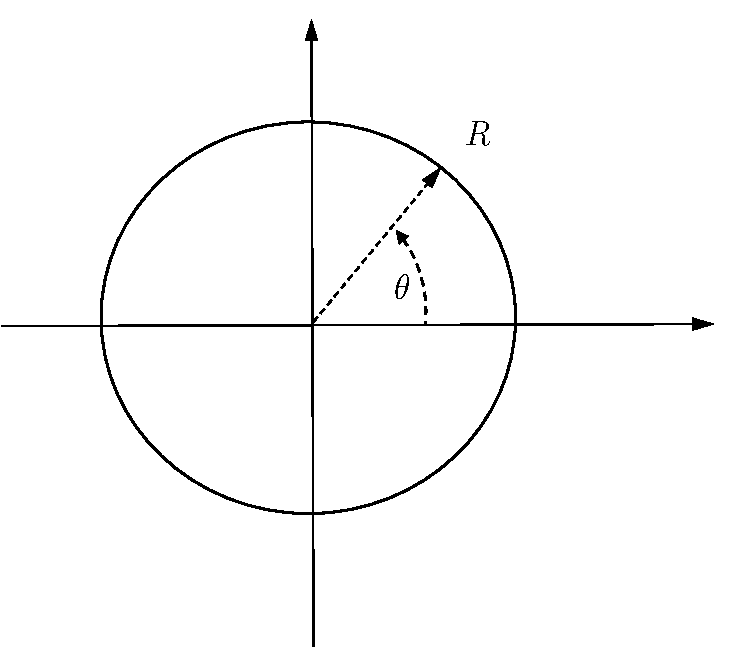
\includegraphics[width=\linewidth]{./chap2_preliminaries/figures/so_2}
  \caption{Visualization of $SO(2)$ as a point on the unit circle in $\mathbb{R}^2$.}
  \label{fig:so_2}  
\end{marginfigure}

The Lie algebra associated with $SO(2)$ is the set
\[
\so(2) = \left\{ M = \begin{pmatrix} 0 & -\theta \\ \theta & 0 \end{pmatrix} ~|~ \theta\in\mathbb{R} \right\},
\]
i.e., the set of skew-symmetric matrices in $\mathbb{R}^{2\times 2}$.  Define the ``wedge'' and ``vee'' operators as
\begin{align*}
\theta^\wedge &= \begin{pmatrix} 0 & -\theta \\ \theta & 0 \end{pmatrix} \\
\begin{pmatrix} 0 & -\theta \\ \theta & 0 \end{pmatrix}^\vee &= \theta.
\end{align*}
By straightforward manipulation, we can show that 
\begin{align*}
\exp(\theta^\wedge) &= I + \theta^\wedge + \frac{1}{2!}(\theta^\wedge)^2 + \frac{1}{3!}(\theta^\wedge)^3 + \dots \\
&= \begin{pmatrix} \cos\theta & -\sin\theta \\ \sin\theta & \cos\theta \end{pmatrix}.
\end{align*}
Similarly, the $\log$ of an element of $SO(2)$ is given by
\[
\log(R) = \cos^{-1}\left(\frac{\trace{R}}{2}\right)^\wedge.
\]
It is important to note that 
\begin{align*}
\exp: &~ \se(2) \to SO(2) \\	
\log: &~ SO(2) \to \se(2),
\end{align*}
therefore it is straightforward to move back and forth between the Lie group $SO(2)$ and its Lie algebra $\so(2)$.  Note that the exponential is a many-to-one map, but that the logarithm maps elements of $SO(2)$ onto only a subset of $\so(2)$ represented by $[0,\pi]$.

It is interesting to note that $\so(2)$ is a linear vector space since linear combinations of elements in $\so(2)$ are also elements of $\so(2)$, i.e.,
\[
a\begin{pmatrix} 0 & -\theta \\ \theta & 0 \end{pmatrix} + b\begin{pmatrix} 0 & -\psi \\ \psi & 0 \end{pmatrix} = \begin{pmatrix} 0 & -(a\theta+b\psi) \\ (a\theta+b\psi) & 0 \end{pmatrix}.
\]
Note also that $\so(2)$ only has dimension of one, and that its elementary basis matrix is 
\[
J_1 = \begin{pmatrix} 0 & -1 \\ 1 & 0 \end{pmatrix}.
\]
In Lie group lingo, the basis vector $J_1$ is called the generator of $SO(2)$, because any element of $SO(2)$ can be generated by the exponential of a linear combination of the generators, in our case, for any $M$, there exists a $\theta$ such that
\[
M = \exp(\theta J_1).
\]

Taking the derivative of $M\in SO(2)$ gives
\begin{align*}
\frac{d}{dt}\begin{pmatrix} \cos\theta & -\sin\theta \\ \sin\theta & \cos\theta \end{pmatrix} &=
	\begin{pmatrix} -\dot{\theta}\sin\theta & -\dot{\theta}\cos\theta \\ \dot{\theta}\cos\theta & -\dot{\theta}\sin\theta \end{pmatrix} \\
	&= \begin{pmatrix} \cos\theta & -\sin\theta \\ \sin\theta & \cos\theta \end{pmatrix} \begin{pmatrix} 0 & -\dot{\theta} \\ \dot{\theta} & 0 \end{pmatrix},
\end{align*}
or in other words
\[
\dot{R} = R\dot{\theta}^\wedge.
\]
If we define $\omega = \dot{\theta}$, then
\begin{equation}\label{eq:diff_eq_so_2}
\dot{R} = R\omega^\wedge,
\end{equation}
and the solution (as seen in previous sections) is
\[
R(t) = R(t_0)\exp\left(\int_{t_0}^t \omega(\tau)d\tau\right)^\wedge.
\]

Considering the differential equation $\dot{R}=R\omega^\wedge$ note that the right hand side of the equation represents a vector in the vector space that is tangent to $SO(2)$ at element $R$.  This can be visualized in Figure~\ref{fig:tangent_space_SO_2}.  Note that the tangent space is just a rotation by $R$ of the tangent space at the identity element $I$.  The tangent space at $I$ is simply $\se(2)$, which is the Lie algebra.
\begin{marginfigure}[1in]
  \centering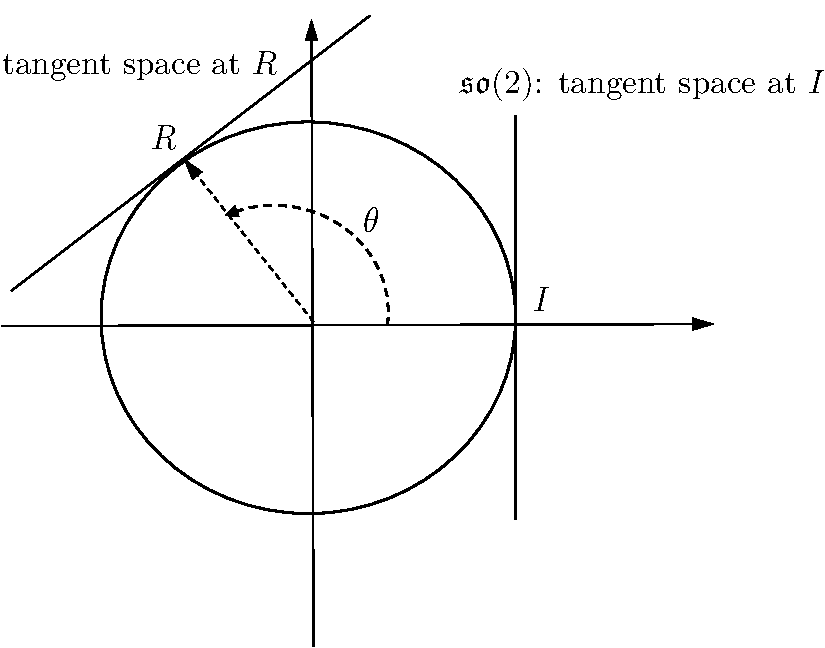
\includegraphics[width=\linewidth]{./chap2_preliminaries/figures/tangent_space_SO_2}
  \caption{Visualization of $\so(2)$ and the tangent space to $SO(2)$.}
  \label{fig:tangent_space_SO_2}  
\end{marginfigure}
This is a general property of the Lie algebra of a Lie group, it is the tangent space at the identity element.

Note also that if Equation~\eqref{eq:diff_eq_so_2} is multiplied on the left by a constant matrix $Q\in SO(2)$, and we let $S=QR$, then
\begin{align*}
\dot{S} &= \dot{QR} \\
        &= Q\dot{R} \\
        &= QR\omega^\wedge \\
        &= S\omega^\wedge.
\end{align*}
Therefore $S=QR$ satisfies exactly the same differential equation as $R$.  Dynamics that not affected by a left multiplication of a element of the group are said to be {\em left-invariant}.  Similarly, if $Q=R^\top$, then $Q$ satisfies $\dot{Q} = -\omega^\wedge Q$, which can be multiplied on the right by a constant matrix without affecting the dynamics, and are said to be {\em right-invariant}.

Note that $SO(2)$ is a one-dimensional group because it can be described by a single parameter $\theta$.  
We typically think of elements of $SO(2)$ as rotation matrices that rotate vectors.  Therefore, associated with the vector $\wbf\in\mathbb{R}^2$, we can define the {\em group action}
\[
f_{\wbf}(R) = R\wbf,
\]
where the output of $f(R)$ is a vector that represents a rotation of $\wbf$.  However, there is a slightly different perspective here, because we think of $f$ as a function of the group element $R$, with a fixed $\wbf$, instead of as a function of $\wbf$.  It is natural to ask whether we can take the Jacobian of the group action $f$ with respect to the group element $R$.  

Toward that end, recall that the Jacobian of a function $g: \mathbb{R}^n\to\mathbb{R}^m$ is given by
\[
\frac{\partial g}{\partial x} = \lim_{\varepsilon\to 0} \begin{pmatrix} \frac{g(x+\varepsilon\ebf_1)}{\varepsilon} & \dots & \frac{g(x+\varepsilon\ebf_n)}{\varepsilon}\end{pmatrix},
\]
where the $i^{th}$ row describes how  $g$ changes with incremental changes in $x$ along the basis vector $\ebf_i$.  We can define the $\frac{\partial f}{\partial R}$ similarly, where the $i^{th}$ row of the Jacobian would describe how the group action $f_\wbf(R)$ changes incrementally as $R$ changes incrementally along the basis vector, or generator $J_i$.  In our case, there is only one generator, thus
\begin{align*}
\frac{\partial f}{\partial R} &= \frac{\partial R\wbf}{\partial R} \\
  &= \lim_{\varepsilon\to 0} \frac{R\exp(\varepsilon J_1)\wbf - R\wbf}{\varepsilon} \\
  &= \lim_{\varepsilon\to 0} \frac{R\left(I + \varepsilon J_1 + \frac{\varepsilon^2}{2!}J_1^2 + \dots \right)\wbf - R\wbf}{\varepsilon} \\
  &= \lim_{\varepsilon\to 0} \frac{\varepsilon RJ_1\wbf}{\varepsilon} \\
  &= R J_1 \wbf.
\end{align*}
Note that $\frac{\partial f}{\partial R}$ is a $2\times 1$ vector that because $f_\wbf(R)$ maps to $\mathbb{R}^2$ (number of rows), and there is only one generator function (number of columns).
Therefore, knowing the structure (dimension and generators) of the Lie algebra is critical to the process of taking Jacobians of group actions.

\rwbcomment{add discussion on adjoints.}


%+++++++++++++++++++++++++++++++++++++++++++++++++++++++
\subsection{The Lie group $SO(3)$}

From the previous section, it should be clear that $SO(3)$ is a Lie group with matrix multiplication as the group operator.  The associated Lie algebra is $\so(3)$, the set of $3\times 3$ skew-symmetric matrices.

The exponential and logarithm functions are defined in Lemmas~\ref{lem:rodrigues_exponential} and~\ref{lem:matrix_log}.  The ``wedge'' and ``vee'' operations are defined as $\omegabf^\wedge = \ss{\omegabf}$ and Equation~\eqref{eq:vee_so_3}. Since $\Omega\in\so(3)$ implies that
\[
\Omega = \begin{pmatrix} 0 & -c & b \\ c & 0 & -b \\ -b & a & 0 \end{pmatrix},
\]
the basis vectors for $\so(3)$, or in other words, the generators for $SO(3)$ are
\begin{align*}
J_{1} & =\ebf_{1}^\wedge = \begin{pmatrix}0 & 0 & 0\\
0 & 0 & -1\\
0 & 1 & 0
\end{pmatrix}, & J_{2} &= \ebf_2^\wedge = \begin{pmatrix}0 & 0 & 1\\
0 & 0 & 0\\
-1 & 0 & 0
\end{pmatrix}, & J_{3} &= \ebf_3^\wedge = \begin{pmatrix}0 & -1 & 0\\
1 & 0 & 0\\
0 & 0 & 0
\end{pmatrix}.
\end{align*}
Therefore $\Omega\in\so(3)$ implies that
\[
\Omega = aJ_1 + bJ_2 + cJ_3,
\]
and any element $R\in SO(3)$ can be expressed as
\[
R = \exp\left( aJ_1 + bJ_2 + cJ_3 \right)
\]

If the group action is defined as $f_\wbf(R) = R\wbf$, then the Jacobian of $f$ with respect to $R$ can be computed as
\begin{align*}
\frac{\partial f}{\partial R} &= \lim_{\varepsilon \to 0} \begin{pmatrix} 
 	\frac{R\exp(\varepsilon J_1)\wbf - R\wbf}{\varepsilon} & 
 	\frac{R\exp(\varepsilon J_2)\wbf - R\wbf}{\varepsilon} &
 	\frac{R\exp(\varepsilon J_3)\wbf - R\wbf}{\varepsilon}
 \end{pmatrix} \\
 &= \lim_{\varepsilon \to 0} \begin{pmatrix} 
 	\frac{\varepsilon RJ_1\wbf}{\varepsilon} & 
 	\frac{\varepsilon RJ_2\wbf}{\varepsilon} &
 	\frac{\varepsilon RJ_3\wbf}{\varepsilon}
 \end{pmatrix}
  = R\begin{pmatrix} 
 	\ebf_1^\wedge\wbf & 
 	\ebf_2^\wedge\wbf & 
 	\ebf_3^\wedge\wbf 
 \end{pmatrix} \\
 &= R\begin{pmatrix} 
 	\wbf^\wedge\ebf_1 & 
 	\wbf^\wedge\ebf_2 & 
 	\wbf^\wedge\ebf_3 
 \end{pmatrix} 
  = R\wbf^\wedge \begin{pmatrix} 
 	\ebf_1 & 
 	\ebf_2 & 
 	\ebf_3 
 \end{pmatrix}\\
   &= -R\wbf^\wedge.
\end{align*}

\rwbcomment{Need to explain other Jacobians in table at end of section.}
\rwbcomment{Need to explain adjoint.}
\rwbcomment{Need to explain right Jacobian vs. left Jacobian.}


%
%
%As mentioned before, all members of a Lie group can be created by
%computing the exponential of a linear combination of the generators.
%Furthermore, because the generators are orthogonal, $\so\left(3\right)$
%is isomorphic to $\mathbb{R}^{3}$. Therefore, to keep things concise, we
%can actually form a vector whose coefficients are then multiplied
%by the generators. In the case of $SO(3)$, this is the
%same as computing the skew-symmetric matrix of a vector. But in general,
%the $\left(\cdot\right)^{\wedge}$ and $\left(\cdot\right)^{\vee}$
%notation is used to indicate this mapping. For example, for $\so\left(3\right):$
%
%\begin{align*}
%\left(\vbf^{\wedge}\right) & =\sum_{i}J_{i}\ebf_{i}^{\top}\vbf\\
% & =J_{1}\vbf_{x}+J_{2}\vbf_{y}+J_{3}\vbf_{z}\\
% & =\begin{pmatrix}0 & -\vbf_{z} & \vbf_{y}\\
%\vbf_{z} & 0 & -\vbf_{x}\\
%-\vbf_{y} & -\vbf_{x} & 0
%\end{pmatrix},
%\end{align*}
%
%\[
%\left(\vbf^{\wedge}\right)^{\vee}=\vbf.
%\]
%This notation is used in some literature \cite{Barfoot2019,Sola2019},
%but not in others \cite{Drummond2014,Ethan2019}. Since the two representations
%(the matrix algebra and the vector) are isomorphic, the mapping to
%the matrix Lie Algebra is often skipped notationally, and $\exp\left(\vbf\right)$
%is written while $\exp\left(\vbf^{\wedge}\right)$ would technically
%be more correct. As computing the matrix exponential of $\vbf\in\mathbb{R}^{3}$
%is actually not possible given the definition above, the mapping of
%the vector to the matrix Lie Algebra is implied in literature where
%the mapping is ignored.

%+++++++++++++++++++++++++++++++++++++++++++++++++++++++
\subsection{The Lie group $SE(3)$}

\rwbcomment{rewrite this section}

As mentioned before, $SE(3)$ is the set of rigid body
transforms. Lie Theory as developed by physicists has very little
to say about $SE(3)$, as it is actually a subset of the
set of $4\times4$ matrices, known classically as the Lorentz group.
The Lorentz group (or the complexified version, octonians) are used
to encode not only rigid body transforms, but also the dilation of
space and time due to relativistic effects. In robotics, we can usually
restrict ourselves to time and space-preserving transformations, so
we can use a simplified version of the Lorentz space generators.\footnote{The bottom row of the $4\times4$ matrix is used in the Lorentz group,
whereas is it not used in $SE(3).$ The Lorentz group
generators continue the skew-symmetric pattern we are used to in this
bottom row and right column. For more information about using Lie
groups to model spacetime, \cite{schwichtenberg_2015} is a phenomenal
introductory text to Lie groups in the context of theoretical physics.
It includes a very good explanation of the Lorentz group and its double-cover.} 

The generators of $SE(3)$ are just the basis of infinitesimal
transformations along each degree of freedom.

\begin{align*}
J_{1} & =\begin{pmatrix}0 & 0 & 0 & 0\\
0 & 0 & -1 & 0\\
0 & 1 & 0 & 0\\
0 & 0 & 0 & 0
\end{pmatrix} & J_{2} & =\begin{pmatrix}0 & 0 & 1 & 0\\
0 & 0 & 0 & 0\\
-1 & 0 & 0 & 0\\
0 & 0 & 0 & 0
\end{pmatrix} & J_{3} & =\begin{pmatrix}0 & -1 & 0 & 0\\
1 & 0 & 0 & 0\\
0 & 0 & 0 & 0\\
0 & 0 & 0 & 0
\end{pmatrix}\\
J_{4} & =\begin{pmatrix}0 & 0 & 0 & 1\\
0 & 0 & 0 & 0\\
0 & 0 & 0 & 0\\
0 & 0 & 0 & 0
\end{pmatrix} & J_{5} & =\begin{pmatrix}0 & 0 & 0 & 0\\
0 & 0 & 0 & 1\\
0 & 0 & 0 & 0\\
0 & 0 & 0 & 0
\end{pmatrix} & J_{6} & =\begin{pmatrix}0 & 0 & 0 & 0\\
0 & 0 & 0 & 0\\
0 & 0 & 0 & 1\\
0 & 0 & 0 & 0
\end{pmatrix}.
\end{align*}
The use of these generators defines the $\left(\cdot\right)^{\wedge}$
operator for $SE(3)$ as

\[
\begin{pmatrix}\omegabf\\
\vbf
\end{pmatrix}^{\wedge}=\begin{pmatrix}\ss{\omegabf} & \vbf\\
0 & 0
\end{pmatrix},
\]
and $\left(\cdot\right)^{\vee}$ as the inverse operation.



%+++++++++++++++++++++++++++++++++++++++++++++++++++++++
\subsection{The Lie group $S^3$}

\rwbcomment{rewrite this section}

%++++++++++++++++++++++++++++++++++++++
\subsection{Closed-Form Exponential for $\protect S^{3}$}

Let's start with the definition of the quaternion exponential

\begin{align}
\exp\left(\omegabf^{\wedge}\right) & =\sum_{k=0}^{\infty}\frac{\left(\omegabf^{\wedge}\right)^{k}}{k!}, & \omegabf^{\wedge} & =\begin{pmatrix}0\\
\omegabf
\end{pmatrix}\label{eq:quat_exp_series}
\end{align}
where the term $\left(\qbf\right)^{k}$ refers to multiplying $\qbf$
with itself $\left(\qbf\cdot\qbf\cdot\cdots\right)$ $k$ times. We also
note that

\begin{align*}
\left(\omegabf^{\wedge}\right)^{2} & =\left(\omegabf_{x}i+\omegabf_{y}j+\omegabf_{z}k\right)\cdot\left(\omegabf_{x}i+\omegabf_{y}j+\omegabf_{z}k\right)\\
 & =-\omegabf_{x}^{2}-\omegabf_{d}^{2}-\omegabf_{z}^{2}\\
 & =-\norm{\omegabf}^{2}
\end{align*}
Therefore, if $\theta=\norm{\omegabf}$, then

\begin{align*}
\left(\omegabf^{\wedge}\right)^{2} & =-\theta^{2}, & \left(\omegabf^{\wedge}\right)^{3} & =-\theta^{2}\omegabf^{\wedge} & \left(\omegabf^{\wedge}\right)^{4} & =\theta^{4}\cdots.
\end{align*}
Now, we can rewrite the series in Eq. \ref{eq:quat_exp_series} as

\begin{align}
\exp\left(\omegabf^{\wedge}\right) & =\sum_{k=0}^{\infty}\frac{\left(\omegabf^{\wedge}\right)^{k}}{k!}\nonumber \\
 & =1+\omegabf^{\wedge}-\frac{\theta^{2}}{2!}-\frac{\theta^{2}}{3!}\omegabf^{\wedge}+\frac{\theta^{4}}{4!}+\frac{\theta^{4}}{5!}\omegabf^{\wedge}-\cdots\nonumber \\
 & =1+\frac{\theta}{\theta}\omegabf^{\wedge}-\frac{\theta^{2}}{2!}-\frac{\theta^{3}}{3!\theta}\omegabf^{\wedge}+\frac{\theta^{4}}{4!}+\frac{\theta^{5}}{5!\theta}\omegabf^{\wedge}-\cdots\nonumber \\
 & =\left(1-\frac{\theta^{2}}{2!}+\frac{\theta^{4}}{4!}\cdots\right)+\frac{1}{\theta}\left(\theta-\frac{\theta^{3}}{3!}+\frac{\theta^{5}}{5!}\cdots\right)\omegabf^{\wedge}\nonumber \\
 & =\cos\left(\theta\right)+\frac{\sin\left(\theta\right)}{\theta}\omegabf^{\wedge}.\label{eq:quat_exp}
\end{align}
As with the rotation matrix exponential, we will want to use the Taylor
series approximation if $\theta\approx0$ to avoid numerical errors.
(See Table \ref{tab:taylor_series}).

Computing the closed-form logarithm is done by inverting Eq. \ref{eq:quat_exp}
and is given by

\[
\log\left(\qbf\right)=\textnormal{atan2}\left(\norm{\vec{\qbf}},q_{0}\right)\frac{\qbf}{\norm{\vec{\qbf}}}.
\]
Because of the fact that quaternion dynamics have a $\frac{1}{2}$
in front of them (See Eq. \ref{eq:quaternion_dynamics}), it is common
practice in both physics and robotics applications to embed the $\frac{1}{2}$
into the $\exp$ function itself such that\footnote{You might recognize this as the axis-angle conversion to unit quaternions
(Eq. \ref{eq:quat_axis_angle})}

\[
\boxed{\exp\left(\omegabf\right)=\cos\left(\frac{\norm{\omegabf}}{2}\right)+\sin\left(\frac{\norm{\omegabf}}{2}\right)\frac{\omegabf}{\norm{\omegabf}}}
\]

\[
\boxed{\log\left(\qbf\right)=2\tan^{-1}\left(\frac{\norm{\vec{\qbf}}}{q_{0}}\right)\cdot\frac{\vec{\qbf}}{\norm{\vec{\qbf}}}.}
\]
This is actually the same as if we redefined the generators of the
unit quaternion to all be $\frac{1}{2}J_{i}$. This is fine, and totally
proper, however we just need to be explicit about this choice.

\subsection{The Generators of $\protect SU\left(2\right)/\protect S^{3}$}

We can follow the same procedure that we performed to derive the generators
of $SO(3)$ to get the generators of $ SU\left(2\right)/ S^{3}$.
First, let's start with the conditions of $ SU\left(2\right)$

\[
U^{\dagger}U=UU^{\dagger}=1\qquad\qquad\det\left(U\right)=1.
\]
Now, as before, let us write these conditions in terms of the generators,
and use BCH in tandem with the fact that $\left[U^{\dagger},U\right]=0$
to get

\begin{align}
U^{\dagger}U & =1\nonumber \\
\left(\exp\left(iJ\right)\right)^{\dagger}\exp\left(iJ\right) & =1\nonumber \\
\exp\left(-iJ^{\dagger}\right)\exp\left(iJ\right) & =1\nonumber \\
\exp\left(-iJ^{\dagger}+iJ+\frac{1}{2}\text{\ensuremath{\left[J^{\dagger},J\right]}}\right)+\dots & =1 & \textnormal{(BCH)}\nonumber \\
\exp\left(-iJ^{\dagger}+iJ\right) & =1\nonumber \\
-iJ^{\dagger}+iJ & =0\nonumber \\
J^{\dagger} & =J.\label{eq:HermetianSU2}
\end{align}
Now, if we look at the second condition, (again, leveraging $\det\left(\exp\left(A\right)\right)=\exp\left(\textnormal{tr}\left(A\right)\right)$),
we can see

\begin{align}
\det\left(\exp\left(iJ\right)\right) & =1\nonumber \\
\exp\left(i\textnormal{tr}\left(J\right)\right) & =1\nonumber \\
\textnormal{tr}\left(J\right) & =0.\label{eq:tracelessSU2}
\end{align}
So the generators must be Hermetian (Eq. \ref{eq:HermetianSU2}),
and traceless (Eq. \ref{eq:tracelessSU2}) complex $2\times2$ matrices.
The standard basis for this set is

\begin{align*}
J_{1} & =\begin{pmatrix}0 & 1\\
1 & 0
\end{pmatrix} & J_{2} & =\begin{pmatrix}0 & -i\\
i & 0
\end{pmatrix} & J_{3} & =\begin{pmatrix}1 & 0\\
0 & -1
\end{pmatrix}.
\end{align*}
This choice of generators corresponds with infinitesimal rotations
in $ SU\left(2\right),$ and because of the isomorphism between $ SU\left(2\right)$
and $ S^{3}$ (unit quaternions), we have also just derived the generators
for unit quaternions as well:

\begin{align*}
J_{1} & =i & J_{2} & =j & J_{3} & =k.
\end{align*}
This means that the $\left(\cdot\right)^{\wedge}$ operations for
$ SU\left(2\right)$ and $ S^{3}$ are given as

\[
\omegabf^{\wedge}=\begin{pmatrix}\omegabf_{z} & \omegabf_{x}-\omegabf_{y}i\\
\omegabf_{x}+\omegabf_{y}i & \omegabf_{z}
\end{pmatrix},
\]
and

\[
\omegabf^{\wedge}=\begin{pmatrix}0\\
\omegabf
\end{pmatrix},
\]
respectively, while the $\left(\cdot\right)^{\vee}$operator is defined
as the inverse of either operation.

There is a very interesting relationship between $\su\left(2\right)$
and $\so\left(3\right)$. Both algebras have the following property:

\begin{align*}
\left[J_{1},J_{2}\right] & =J_{3} & \left[J_{2},J_{1}\right] & =-J_{3}\\
\left[J_{2},J_{3}\right] & =J_{1} & \left[J_{3},J_{2}\right] & =-J_{1}\\
\left[J_{3},J_{1}\right] & =J_{2} & \left[J_{1},J_{3}\right] & =-J_{2}.
\end{align*}
It turns out, this is indicative of a more fundamental result. One
can say that $ SU\left(2\right)$ and $SO(3)$ have the
same Lie algebra, because we define Lie algebras by their Lie bracket.
Forgive the extended quotation, but this summary from \emph{Physics
From Symmetry\cite{schwichtenberg_2015}} explains this concept in
detail, as well as giving a very nice motivation for why we use Lie
Algebras in the first place.
\begin{quote}
There is precisely one simply-connected Lie group corresponding to
each Lie algebra. This simply-connected group can be thought of as
the \textquotedbl mother\textquotedbl{} of all those groups having
the same Lie algebra, because there are maps to all other groups with
the same Lie algebra from the simply connected group, but not vice
versa. We could call it the mother group of this particular Lie algebra,
but mathematicians tend to be less dramatic and call it the covering
group. All other groups having the same Lie algebra are said to be
covered by the simply connected one. $SU(2)$ is the double cover
of $SO(3)$. This means there is a two-to-one map from $SU(2)$ to
$SO(3)$.

Furthermore, $SU(2)$ is the three sphere, which is a simply connected
manifold. Therefore, we have found the \textquotedbl most important\textquotedbl{}
group belonging to the Lie algebra. We can get all other groups belonging
to this Lie algebra through maps from $SU(2)$.

We can now understand what manifold $SO(3)$ is. The map from $SU(2)$
to $SO(3)$ identifies with two points of $SU(2)$, one point of $SO(3)$.
Therefore, we can think of $SO(3)$ as the top half of $ S^{3}$

We can see, from the point of view that Lie groups are manifolds that
$SU(2)$ is a more complete object than $SO(3)$. $SO(3)$ is just
\textquotedbl part\textquotedbl{} of the complete object.

...

To describe nature at the most fundamental level, we must use the
covering group, instead of any of the other groups that one can map
to from the covering group. We are able to derive the representations
of the most fundamental group, belonging to a given Lie algebra, by
deriving representations of the Lie algebra. We can then put the matrices
representing the Lie algebra elements (the generators) into the exponential
function to get matrices representing group elements. 

Herein lies the strength of Lie theory. By using pure mathematics
we are able to reveal something fundamental about nature. The standard
symmetry group of special relativity hides something from us {[}the
spin of elementary particles{]}, because it is not the most fundamental
group belonging to this symmetry. The covering group of the Poincar�
group is the fundamental group and therefore we will use it to describe
nature.
\end{quote}
What Schwichtenberg is talking about is the fact that the double cover
of the Lorentz group is able to represent the spin of a particle,
while the standard Lorentz group cannot. This is analogous to the
difference between the use of $ S^{3}/ SU\left(2\right)$ versus $SO(3)$.
In robotics, we are typically unconcerned with the bottom half of
the $ S^{3}$ unit sphere, so there is no fundamental drawback to
using $SO(3)$ like there is in particle physics. However,
there is something about nature and pure mathematics that encodes
rotations in a double cover, and $SO(3)$ only tells us
half of the story.

Finally, it's crucial to realize that the Lie groups arise from and
are defined by the Lie algebra, and therefore by the generators. Not
the other way around. By starting at the generators we can capture
at a more fundamental level what is going on in 3D rotations, and
what the manifold really is. 






\section{The Adjoint as the Jacobian of Group Action}

\rwbcomment{move this stuff up into the previous sections}

\label{sec:ad_as_jacobian}

Most people's first introduction to calculus typically focuses on
computing derivatives. For completeness, we're going to start here
and work our way to computing Jacobians of the Lie Group action. The
formula for computing the derivative of a scalar function $f$, is
given as
%
\sidenote{Note, to be consistent with the vast majority of literature on this
topic, I am using $\varepsilon$ to mean a small perturbation. This
is a separate and distinct concept from $\epsilon,$ the dual number.}
%
\[
\frac{\partial f}{\partial x}=\lim_{\varepsilon\to0}\frac{1}{\varepsilon}\left(f\left(x+\varepsilon\right)-f\left(x\right)\right).
\]
In conversational English, this means, ``How does the output of the
function $f$ change if I bump the input a tiny bit?'' This is very
naturally adapted for a vector function $g\in\mathbb{R}^{m}\to\mathbb{R}^{n}$
as

\begin{align*}
\frac{\partial g}{\partial\xbf} & =\lim_{\varepsilon\to0}\frac{1}{\varepsilon}\begin{bmatrix}\deltabf_{1}\left(\xbf,\varepsilon\right) & \deltabf_{2}\left(\xbf,\varepsilon\right)\cdots\deltabf_{m}\left(\xbf,\varepsilon\right)\end{bmatrix}\in\mathbb{R}^{n\times m}\\
\deltabf_{i}\left(\xbf,\varepsilon\right) & =g\left(\xbf+\ebf_{i}\varepsilon\right)-g\left(\xbf\right)
\end{align*}
Again, in conversational English, we're saying that $g$ is a function
that takes in $m$-vectors and produces $n$-vectors. We want to know
what $g$ looks like along each of the input axes, so we're going
to make a matrix where each column is the derivative along each of
these directions. This is known as the Jacobian matrix, and can also
be interpreted as, ``If I change the input in some way, what does
it do to the output?'' For example, if I go further along the $\ebf_{1}$-axis,
would I expect the output to go up or down? This would be captured
in the first column of the Jacobian. This relationship lets us look
at Jacobians as a sort of mapping from input space to output space,
and lets us quickly compute how changes in input should affect the
output of the function $g$.

The concept of differentiation works quite naturally with Lie groups
as well. For example, consider the case of some function $h\in SE(3)\to\mathbb{R}^{n}.$
What we want is a matrix that tells us how the output of $h$ behaves
as we tweak the argument of $h$ along the \emph{generators }of $\se\left(3\right).$
To compute this, we use the fact that every member of the group can
be described by the exponential of some linear combination of generators,
as in

\begin{align*}
T & =\exp\left(\xbf^{\wedge}\right), & \xbf^{\wedge} & =\log\left(T\right).
\end{align*}
When we write it this way, we can see how we might perturb $\xbf$ (and
therefore, $T$) in the $J_{i}$ direction:

\begin{align*}
T_{i}^{+} & =\exp\left(\xbf^{\wedge}+J_{i}\varepsilon\right)\\
 & =T\cdot\exp\left(J_{i}\varepsilon\right).
\end{align*}
Next, we need to think about how we might compute the difference between
$T_{i}^{+}$ and the original $T$. Again, looking to the Lie Algebra,
we should expect the difference $\deltabf_{i}\in\se\left(3\right)$ to
be

\begin{align}
\exp\left(\deltabf_{i}\right) & =T\cdot\exp\left(J_{i}\varepsilon\right)\cdot\exp\left(-\xbf^{\wedge}\right)\nonumber \\
\deltabf_{i} & =\log\left(T\cdot\exp\left(J_{i}\varepsilon\right)\cdot T^{-1}\right)^{\vee}.\label{eq:adjoint_start}
\end{align}
If we make a matrix out of the six $\deltabf_{i}$ for $\se\left(3\right)$,
take the limit as $\varepsilon\to0$ and attach coordinate frames
to our transform $T_{a}^{b}$, then we get a $6\times6$ matrix that
tells us how things change along the generators in the $b$ frame
if we perturb along the generators the $a$ frame. This has a special
name--the Adjoint--and it just so happens to be the Jacobian of
the group action by a member of the group.

We can come at the Adjoint in another way: because the Adjoint is
the Jacobian of the group action of a Lie group, we can use it to
map vectors from the ``output'' of a group action to the ``input'',
and vice-versa. In mathematical terms\footnote{for the rest of this section, I'm dropping the $\left(\cdot\right)^{\wedge}$
so we can focus on the coordinate frame notation. The mapping from
the vector to algebra should be implied by context.}:

\[
T\cdot\exp\left(\deltabf\right)=\exp\left(\Ad_{T}\cdot\deltabf\right)\cdot T.
\]
See how we have ``moved'' $\deltabf$ from the ``input'' of $T$ (the
right side) to the ``output'' (the left side)? If we attach coordinate
frames to $T$ this becomes even more clear: 

\begin{align}
T_{a}^{b}\cdot\exp\left(\deltabf^{a}\right) & =\exp\left(\Ad\left(T_{a}^{b}\right)\cdot\deltabf^{a}\right)\cdot T_{a}^{b}.\nonumber \\
 & =\exp\left(\deltabf^{b}\right)\cdot T_{a}^{b}.\label{eq:adjoint_show}
\end{align}
The Adjoint transforms $\deltabf$ from $a$ to $b.$

Remember all that talk about left-invariance and right-invariance?
This property of the Adjoint of the Lie Group lets us swap back and
forth however we need to. This is really helpful when computing Jacobians
of complex expressions involving Lie Groups.

\section{Closed-Form Expressions for the Adjoint}

In this section, I'm going to derive the Adjoint for each of our four
Lie Groups, but before we do that,\emph{ }let's first talk about a
concrete example of where the Adjoint is useful. 

Let's consider some kind of nonlinear controller that is computing
error on the Lie Algebra of $SE(3)$, where we have some
desired state $\check{T}$ and our current state $T.$ We're going
to form some control law around the error between these two states.
Naturally, we want to use linear algebra as the backbone of our implementation,
so we'd like to use $\se\left(3\right)^{\vee}$ to represent our error.
We could compute the error in one of 4 ways:

\begin{align*}
\deltabf_{a}^{\check{a}} & =\log\left(\check{\left(T_{a}^{b}\right)}^{-1}\cdot T_{a}^{b}\right)\\
\deltabf_{b}^{\check{b}} & =\log\left(\check{T_{a}^{b}}\cdot\left(T_{a}^{b}\right)^{-1}\right)\\
\deltabf_{\check{a}}^{a} & =\log\left(\left(T_{a}^{b}\right)^{-1}\cdot\check{T_{a}^{b}}\right)\\
\deltabf_{\check{b}}^{b} & =\log\left(\left(T_{a}^{b}\right)\cdot\left(\check{T}_{a}^{b}\right)^{-1}\right).
\end{align*}
The choice of error depends largely on which frames are moving, and
which are not. Let's assume that in this case the $a$ frame is shared
between the transform (i.e. perhaps $a$ refers to the inertial frame),
and that the $b$ and $\check{b}$ frames are the current and desired
body frame of a robot. The goal of the controller in this case is
to make $b=\check{b}.$ In this case, it makes the most sense to define
our error as one of the following two options (or else the coordinate
frames will not match up):

\begin{align*}
\deltabf_{b}^{\check{b}} & =\log\left(\check{T_{a}^{b}}\cdot\left(T_{a}^{b}\right)^{-1}\right),\\
\deltabf_{\check{b}}^{b} & =\log\left(T_{a}^{b}\cdot\left(\check{T}_{a}^{b}\right)^{-1}\right).
\end{align*}
Driving either of these errors to zero will achieve our control objectives.
However, watch what happens when we want to compute the Jacobian of
our error with respect to our current state. We can find these Jacobians
using the chain rule: 

\begin{align*}
\frac{\partial}{\partial T_{a}^{b}}\deltabf_{b}^{\check{b}} & =\left.\frac{\partial\log\left(\xbf\right)}{\partial\xbf}\right|_{\xbf=\left(T_{a}^{b}\cdot\left(T_{a}^{\check{b}}\right)\right)}\cdot\frac{\partial}{\partial T_{a}^{b}}\left(\check{T_{a}^{b}}\cdot\left(T_{a}^{b}\right)^{-1}\right) & =A\cdot B^{\check{b}}\\
\frac{\partial}{\partial T_{a}^{b}}\deltabf_{\check{b}}^{b} & =\left.\frac{\partial\log\left(\xbf\right)}{\partial\xbf}\right|_{\xbf=\left(T_{a}^{b}\cdot\left(T_{a}^{\check{b}}\right)\right)}\cdot\frac{\partial}{\partial T_{a}^{b}}\left(T_{a}^{b}\cdot\left(\check{T_{a}^{b}}\right)^{-1}\right) & =A\cdot B^{b}
\end{align*}

The expression for $A$ is in Table \ref{tab:lie_identities_group_vector-se3},
and it's the same for both parameterizations. However, we are left
with the two $B$ expressions. In the first case, we have to go through
our desired state to get to the current state. This isn't too bad,
we just look at Table \ref{tab:lie_identities_group_operations} to
get (using the left Jacobian):

\begin{align*}
B^{\check{b}} & =\frac{\partial}{\partial T_{a}^{b}}\left(\check{T_{a}^{b}}\cdot\left(T_{a}^{b}\right)^{-1}\right)\\
 & =-\Ad\left(\check{T_{a}^{b}}\cdot\left(T_{a}^{b}\right)^{-1}\right)
\end{align*}
for the first cast, and

\begin{align*}
B^{b} & =\frac{\partial}{\partial T_{a}^{b}}\left(T_{a}^{b}\cdot\left(\check{T_{a}^{b}}\right)^{-1}\right)\\
 & =I\in\mathbb{R}^{6\times6}.
\end{align*}
for the second. Having a closed form expression for the Adjoint makes
computing these kinds of expressions very straight-forward. 

Most modern forms of control and estimation rely heavily on quickly-computed
Jacobians. With a table of Jacobians for exp, log, Ad and a few other
Lie group expressions, plus the Matrix Cookbook \cite{Petersen2012},
it's pretty easy to chain-rule out even the hairiest Jacobians pretty
quickly to get analytical expressions. Appendix \ref{sec:Tables}
contains most of these Jacobians for easy reference.

\subsection{Adjoint for $SO(3)$}

For all four Lie groups, we can derive the Adjoint by finding the
closed-form expression of Eq. \ref{eq:adjoint_start}. $SO(3)$
is quite easy:

\begin{align*}
\Ad\left(R\right) & =\lim_{\varepsilon\to0}\frac{1}{\varepsilon}\begin{bmatrix}R\cdot\exp\left(J_{1}\varepsilon\right)\cdot R^{-1} & \cdots\end{bmatrix}\\
 & =\lim_{\varepsilon\to0}\frac{1}{\varepsilon}\begin{bmatrix}R\cdot\left(I+\ss{\ebf_{1}\epsilon}+\cdots\right)\cdot R^{-1} & \cdots\end{bmatrix}\\
 & =\lim_{\varepsilon\to0}\frac{1}{\varepsilon}\begin{bmatrix}R\cdot R^{-1}+R\cdot\ss{\ebf_{1}\epsilon}\cdot R^{-1} & \cdots\end{bmatrix}\\
 & =\begin{bmatrix}R\cdot\ss{\ebf_{1}}\cdot R^{-1} & \cdots\end{bmatrix} & R\cdot R^{-1}=I\\
 & =\begin{bmatrix}\ss{R\ebf_{1}} & \ss{R\ebf_{2}} & \ss{R\ebf_{3}}\end{bmatrix} & \textnormal{(Eq. \ref{eq:skew_trick_2})}\\
 & =R
\end{align*}
We see here that $SO(3)$ is \emph{self-adjoint}, and
it makes sense why. Consider an $SO(3)$ version of Eq.
\ref{eq:adjoint_show}. Rotating the vector is the natural way to
transform $\deltabf$ from the $a$ frame to the $b$ frame.

\[
\boxed{\Ad\left(R\right)=R}
\]


\subsection{Adjoint for Unit Quaternions}

Remember, the Adjoint action is given by 

\[
\Ad=\lim_{\varepsilon\to0}\frac{1}{\varepsilon}\begin{bmatrix}\log\left(\qbf\cdot\exp\left(J_{1}\varepsilon\right)\cdot\qbf^{-1}\right) & \cdots\end{bmatrix}.
\]
In the case of unit quaternions, we can see that they too, are self-adjoint.
To compute the adjoint of a quaternion, all we need to do is pre-
and post-multiply a pure quaternion of the lie algebra member by the
quaternion. 

\[
\Ad\left(\qbf\right)=\qbf\cdot\deltabf\cdot\qbf^{-1}.
\]
However, sometimes we might want the matrix form of the adjoint. This
can be computed as follows:

\begin{align*}
 & =\lim_{\varepsilon\to 0}\frac{1}{\varepsilon}\begin{bmatrix}\log\left(\qbf\cdot\begin{pmatrix}0\\
\ebf_{1}\sin\left(\frac{\varepsilon}{2}\right)
\end{pmatrix}\cdot\qbf^{-1}\right) & \cdots\end{bmatrix}\\
 & =\lim_{\varepsilon\to 0}\frac{1}{\varepsilon}\begin{bmatrix}\log\begin{pmatrix}0\\
\frac{R^{\top}\ebf_{1}\varepsilon}{2}
\end{pmatrix} & \cdots\end{bmatrix}\\
 & =\lim_{\varepsilon\to 0}\frac{1}{\varepsilon}\begin{bmatrix}R^{\top}\ebf_{1}\varepsilon & R^{\top}\ebf_{2}\varepsilon & R^{\top}\ebf_{3}\varepsilon\end{bmatrix}\\
 & =R^{\top}.
\end{align*}
You could probably come up with this only just from intuition as well.
If you remember that quaternions and rotation matrices share a Lie
Algebra, and that the order of concatenation is backwards, then $R^{\top}$
is the logical choice.

\[
\boxed{\Ad\left(\qbf\right)=R^{\top}\left(\qbf\right)}
\]


\subsection{Adjoint for $SE(3)$}

Computing this adjoint is more complicated than pure rotation. Unfortunately,
$SE(3)$ isn't self-adjoint,\footnote{This should be pretty obvious, seeing as $\se\left(3\right)$ is 6-dimensional
while $SE(3)$ is a group of $4\times4$ matrices.} so the limit gets a little more hairy. We have two main blocks: the
first three generators are the rotation generators, while the last
three are the translation generators. Let's consider these separately.
First, the rotation blocks

\begin{align*}
\Ad_{1-3} & =\lim_{\varepsilon\to0}\frac{1}{\varepsilon}\begin{bmatrix}\log\left(T\cdot\exp\left(J_{1}\varepsilon\right)\cdot T^{-1}\right) & \cdots\end{bmatrix}\\
 & =\lim_{\varepsilon\to0}\frac{1}{\varepsilon}\begin{bmatrix}\log\left(T\cdot\begin{bmatrix}\ss{\ebf_{1}\varepsilon} & 0\\
0 & 0
\end{bmatrix}\cdot T^{-1}\right) & \cdots\end{bmatrix}\\
 & =\lim_{\varepsilon\to0}\frac{1}{\varepsilon}\begin{bmatrix}\log\left(\begin{bmatrix}R & \tbf\\
0 & 1
\end{bmatrix}\cdot\begin{bmatrix}\ss{\ebf_{1}\varepsilon} & 0\\
0 & 0
\end{bmatrix}\cdot\begin{bmatrix}R^{\top} & -R^{\top}\tbf\\
0 & 1
\end{bmatrix}\right) & \cdots\end{bmatrix}\\
 & =\lim_{\varepsilon\to0}\frac{1}{\varepsilon}\begin{bmatrix}\log\left(\begin{bmatrix}R\ss{\ebf_{1}\varepsilon} & 0\\
0 & 0
\end{bmatrix}\cdot\begin{bmatrix}R^{\top} & -R^{\top}\tbf\\
0 & 1
\end{bmatrix}\right) & \cdots\end{bmatrix}\\
 & =\lim_{\varepsilon\to0}\frac{1}{\varepsilon}\begin{bmatrix}\log\left(\begin{bmatrix}R\ss{\ebf_{1}\varepsilon}R^{\top} & -R\ss{\ebf_{1}\varepsilon}R^{\top}\tbf\\
0 & 0
\end{bmatrix}\right) & \cdots\end{bmatrix}\\
 & =\lim_{\varepsilon\to0}\frac{1}{\varepsilon}\begin{bmatrix}\log\left(\begin{bmatrix}\ss{R\ebf_{1}\varepsilon} & -\ss{R\ebf_{1}\varepsilon}\tbf\\
0 & 0
\end{bmatrix}\right) & \cdots\end{bmatrix} & \textnormal{(Eq. \ref{eq:skew_trick_2})}\\
 & =\lim_{\varepsilon\to0}\frac{1}{\varepsilon}\begin{bmatrix}\log\left(\begin{bmatrix}\ss{R\ebf_{1}\varepsilon} & \ss{\tbf}R\ebf_{1}\varepsilon\\
0 & 0
\end{bmatrix}\right) & \cdots\end{bmatrix} & \textnormal{(Eq. \ref{eq:skew_trick_1})}\\
 & =\lim_{\varepsilon\to0}\frac{1}{\varepsilon}\begin{bmatrix}R\varepsilon\\
\ss{\tbf}R\varepsilon
\end{bmatrix}\\
 & =\begin{bmatrix}R\\
\ss{\tbf}R
\end{bmatrix}.
\end{align*}
Now for the translation blocks

\begin{align*}
\Ad_{4-6} & =\lim_{\varepsilon\to0}\frac{1}{\varepsilon}\begin{bmatrix}\log\left(T\cdot\exp\left(J_{4}\varepsilon\right)\cdot T^{-1}\right) & \cdots\end{bmatrix}\\
 & =\lim_{\varepsilon\to0}\frac{1}{\varepsilon}\begin{bmatrix}\log\left(\begin{bmatrix}R & \tbf\\
0 & 1
\end{bmatrix}\cdot\begin{bmatrix}0 & \ebf_{1}\varepsilon\\
0 & 0
\end{bmatrix}\cdot\begin{bmatrix}R^{\top} & -R^{\top}\tbf\\
0 & 1
\end{bmatrix}\right) & \cdots\end{bmatrix}\\
 & =\lim_{\varepsilon\to0}\frac{1}{\varepsilon}\begin{bmatrix}\log\left(\begin{bmatrix}0 & R\ebf_{1}\varepsilon\\
0 & 0
\end{bmatrix}\cdot\begin{bmatrix}R^{\top} & -R^{\top}\tbf\\
0 & 1
\end{bmatrix}\right) & \cdots\end{bmatrix}\\
 & =\lim_{\varepsilon\to0}\frac{1}{\varepsilon}\begin{bmatrix}\log\left(\begin{bmatrix}0 & R\ebf_{1}\varepsilon\\
0 & 0
\end{bmatrix}\right) & \cdots\end{bmatrix}\\
 & =\lim_{\varepsilon\to0}\frac{1}{\varepsilon}\begin{bmatrix}0 & 0 & 0\\
R\ebf_{1}\varepsilon & R\ebf_{2}\varepsilon & R\ebf_{3}\varepsilon
\end{bmatrix}\\
 & =\begin{bmatrix}0\\
R
\end{bmatrix}.
\end{align*}
We now concatenate these blocks to get the final Adjoint matrix:

\[
\boxed{\Ad\left(T\right)=\begin{pmatrix}R & 0\\
\ss{\tbf}R & R
\end{pmatrix}.}
\]
Note that some literature\cite{Drummond2014,Ethan2019} derives this
block-transposed. All that means is that they define generators 1-3
as the translation generators and 4-6 as the rotation generators.

Before moving on, let's take a second to develop a little bit of intuition
regarding the adjoint when it comes to rigid transforms. Consider
a rod rotating about a fixed origin, as shown in Figure \ref{fig:rotating_adjoint}.
Let us say we have the linear and angular velocity of coordinate frame
$a$, but we want the velocity of coordinate frame $b$. Because the
coordinate frames are fixed by some rigid transform, any angular rate
value of $a$ is the same for $b$, only rotated. However, to compute
the linear velocity of coordinate frame $b$, we must account for
the ``lever arm'' and the angular rate. This is what is going on
in the bottom-left corner of the Adjoint in $SE(3).$ 

\begin{marginfigure}
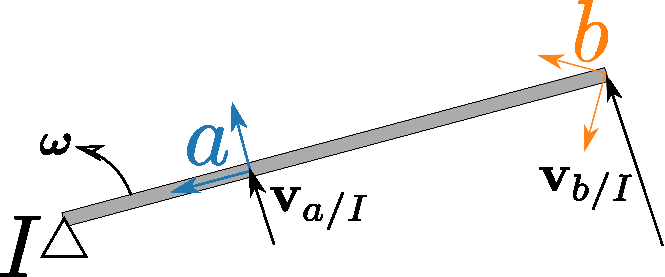
\includegraphics[width=\linewidth]{chap2_preliminaries/figures/rotating_bar}
\caption{Illustration of a rotating rigid body with two coordinate frames.
The Adjoint of $SE(3)$ will convert $\omegabf$
and $\vbf$ from frame $a$ to frame $b$, and account for the
change in translation. }
\label{fig:rotating_adjoint}
\end{marginfigure}

%++++++++++++++++++++++++++++++++++++++++++++++++++++++++
%\subsection{Adjoint of Dual Quaternions}
%
%As with unit quaternions, dual unit quaternions are also self-adjoint:
%
%\[
%\Ad\left(\Gamma\right)=\Gamma\cdot\exp\left(\dbf\right)\cdot\Gamma^{-1}.
%\]
%We have no problem dealing with six-vectors here (the problem with
%$SE(3),$which led us to compute that hairy limit). However,
%just like unit quaternions, we can compute the matrix form of the
%Adjoint using the limit expression. Again, let's split up the generators
%into two groups to help keep things a little more concise
%
%{\small{}
%\begin{align*}
%\Ad_{1-3} & =\lim_{\varepsilon\to0}\frac{1}{\varepsilon}\begin{bmatrix}\log\left(\Gamma\cdot\exp\left(J_{1}\varepsilon\right)\cdot\Gamma^{-1}\right) & \cdots\end{bmatrix}\\
% & =\lim_{\varepsilon\to0}\frac{1}{\varepsilon}\begin{bmatrix}\log\left(\begin{bmatrix}\qbf_{r}\\
%\epsilon\qbf_{d}
%\end{bmatrix}\cdot\begin{bmatrix}\begin{pmatrix}0\\
%\ebf_{1}\sin\left(\frac{\varepsilon}{2}\right)
%\end{pmatrix}\\
%0\epsilon
%\end{bmatrix}\cdot\begin{bmatrix}\qbf_{r}\\
%\epsilon\qbf_{d}
%\end{bmatrix}^{-1}\right) & \cdots\end{bmatrix}\\
% & =\lim_{\varepsilon\to0}\frac{1}{\varepsilon}\begin{bmatrix}\log\left(\begin{bmatrix}\qbf_{r}\\
%\epsilon\qbf_{d}
%\end{bmatrix}\cdot\begin{bmatrix}\ebf_{1}\varepsilon\\
%0\epsilon
%\end{bmatrix}\cdot\begin{bmatrix}\qbf_{r}\\
%\epsilon\qbf_{d}
%\end{bmatrix}^{-1}\right) & \cdots\end{bmatrix} & \sin\varepsilon\to\varepsilon\\
% & =\lim_{\varepsilon\to0}\frac{1}{\varepsilon}\begin{bmatrix}\log\left(\begin{bmatrix}\qbf_{r}\cdot\ebf_{1}^{\wedge}\varepsilon\\
%\epsilon\left(\ebf_{1}^{\wedge}\varepsilon\cdot\qbf_{d}\right)
%\end{bmatrix}\cdot\begin{bmatrix}\qbf_{r}\\
%\epsilon\qbf_{d}
%\end{bmatrix}^{-1}\right) & \cdots\end{bmatrix}\\
% & =\lim_{\varepsilon\to0}\frac{1}{\varepsilon}\begin{bmatrix}\log\left(\begin{bmatrix}\qbf_{r}\cdot\ebf_{1}^{\wedge}\varepsilon\cdot\qbf_{r}^{-1}\\
%\epsilon\left(\qbf_{r}\cdot\ebf_{1}^{\wedge}\varepsilon\cdot\qbf_{d}^{-1}+\qbf_{r}^{-1}\cdot\ebf_{1}^{\wedge}\varepsilon\cdot\qbf_{d}\right)
%\end{bmatrix}\right) & \cdots\end{bmatrix} & \ebf_{1}^{\wedge}=\begin{pmatrix}0\\
%\ebf_{1}
%\end{pmatrix}\\
% & =\lim_{\varepsilon\to0}\frac{1}{\varepsilon}\begin{bmatrix}\log\left(\begin{bmatrix}\qbf_{r}\cdot\ebf_{1}^{\wedge}\varepsilon\cdot\qbf_{r}^{-1}\\
%\epsilon\left(\qbf_{r}\cdot\ebf_{1}^{\wedge}\varepsilon\cdot\begin{pmatrix}\frac{1}{2}\t^{\wedge}\cdot\qbf_{r}\end{pmatrix}^{-1}+\qbf_{r}^{-1}\cdot\ebf_{1}^{\wedge}\varepsilon\cdot\frac{1}{2}\t^{\wedge}\cdot\qbf_{r}\right)
%\end{bmatrix}\right) & \cdots\end{bmatrix}\\
% & =\lim_{\varepsilon\to0}\frac{1}{\varepsilon}\begin{bmatrix}\log\left(\begin{bmatrix}\qbf_{r}\cdot\ebf_{1}^{\wedge}\varepsilon\cdot\qbf_{r}^{-1}\\
%\frac{1}{2}\epsilon\left(\qbf_{r}\cdot\ebf_{1}^{\wedge}\varepsilon\cdot\qbf_{r}^{-1}\cdot\left(-\t^{\wedge}\right)+\qbf_{r}^{-1}\cdot\ebf_{1}^{\wedge}\varepsilon\cdot\t^{\wedge}\cdot\qbf_{r}\right)
%\end{bmatrix}\right) & \cdots\end{bmatrix}\\
% & =\lim_{\varepsilon\to0}\frac{1}{\varepsilon}\begin{bmatrix}\log\left(\begin{bmatrix}\qbf_{r}\cdot\ebf_{1}^{\wedge}\varepsilon\cdot\qbf_{r}^{-1}\\
%\frac{1}{2}\epsilon\left(-\ss{R^{\top}\ebf_{1}\varepsilon}\tbf+R\ss{\ebf_{1}\varepsilon}\tbf\right)
%\end{bmatrix}\right) & \cdots\end{bmatrix} & \textnormal{(Eq. \ref{eq:quat_mult_matrix})}\\
% & =\lim_{\varepsilon\to0}\frac{1}{\varepsilon}\begin{bmatrix}\log\left(\begin{bmatrix}\qbf_{r}\cdot\ebf_{1}^{\wedge}\varepsilon\cdot\qbf_{r}^{-1}\\
%\frac{1}{2}\epsilon\left(-R^{\top}\ss{\ebf_{1}\varepsilon}R\tbf+R\ss{\ebf_{1}\varepsilon}\tbf\right)
%\end{bmatrix}\right) & \cdots\end{bmatrix} & \textnormal{(Eq. \ref{eq:skew_trick_2})}\\
% & =\lim_{\varepsilon\to0}\frac{1}{\varepsilon}\begin{bmatrix}\log\left(\begin{bmatrix}\qbf_{r}\cdot\ebf_{1}^{\wedge}\varepsilon\cdot\qbf_{r}^{-1}\\
%\frac{1}{2}\epsilon\left(R^{\top}\ss{R\t}\ebf_{1}\varepsilon-R\ss{\tbf}\ebf_{1}\varepsilon\right)
%\end{bmatrix}\right) & \cdots\end{bmatrix} & \textnormal{(Eq. \ref{eq:skew_trick_1})}\\
% & =\lim_{\varepsilon\to0}\frac{1}{\varepsilon}\begin{bmatrix}\log\left(\begin{bmatrix}\qbf_{r}\cdot\ebf_{1}^{\wedge}\varepsilon\cdot\qbf_{r}^{-1}\\
%\frac{1}{2}\epsilon\left(\ss{\tbf}R^{\top}\ebf_{1}\varepsilon-R\ss{\tbf}\ebf_{1}\varepsilon\right)
%\end{bmatrix}\right) & \cdots\end{bmatrix} & \textnormal{(Eq. \ref{eq:skew_trick_1})}\\
% & =\begin{bmatrix}R^{\top}\\
%\ss{\tbf}R^{\top}
%\end{bmatrix}.
%\end{align*}
%Whew! Luckily, the translation generators are much easier:}{\small\par}
%
%\begin{align*}
%\Ad_{4-6} & =\lim_{\varepsilon\to0}\frac{1}{\varepsilon}\begin{bmatrix}\log\left(\Gamma\cdot\exp\left(J_{1}\varepsilon\right)\cdot\Gamma^{-1}\right) & \cdots\end{bmatrix}\\
% & =\lim_{\varepsilon\to0}\frac{1}{\varepsilon}\begin{bmatrix}\log\left(\begin{bmatrix}\qbf_{r}\\
%\epsilon\qbf_{d}
%\end{bmatrix}\cdot\begin{bmatrix}0\\
%\ebf_{1}\epsilon
%\end{bmatrix}\cdot\begin{bmatrix}\qbf_{r}\\
%\epsilon\qbf_{d}
%\end{bmatrix}^{-1}\right) & \cdots\end{bmatrix}\\
% & =\lim_{\varepsilon\to0}\frac{1}{\varepsilon}\begin{bmatrix}\log\left(\begin{bmatrix}0\\
%\epsilon\left(\qbf_{r}\cdot\ebf_{q}\varepsilon\right)
%\end{bmatrix}\cdot\begin{bmatrix}\qbf_{r}\\
%\epsilon\qbf_{d}
%\end{bmatrix}^{-1}\right) & \cdots\end{bmatrix}\\
% & =\lim_{\varepsilon\to0}\frac{1}{\varepsilon}\begin{bmatrix}\log\begin{bmatrix}0\\
%\epsilon\left(\qbf_{r}\cdot\ebf_{q}\varepsilon\cdot\qbf_{r}^{-1}\right)
%\end{bmatrix} & \cdots\end{bmatrix}\\
% & =\lim_{\varepsilon\to0}\frac{1}{\varepsilon}\begin{bmatrix}\log\begin{bmatrix}0\\
%\epsilon\left(R^{\top}\ebf_{1}\varepsilon\right)
%\end{bmatrix} & \cdots\end{bmatrix}\\
% & =R^{\top}.
%\end{align*}
%Finally, we can write the full Adjoint for dual quaternions as
%
%\[
%\boxed{\Ad\left(\Gamma\right)=\begin{pmatrix}R^{\top} & 0\\
%\ss{\tbf}R^{\top} & R^{\top}
%\end{pmatrix}},
%\]
%which, unsurprisingly, is the same as the Adjoint of $SE(3)$,
%except with all the rotations transposed (due to the reverse order
%of quaternions rotation with respect to $SO(3).$) Note
%that this is also the matrix inverse of the Adjoint of $SE(3)$. 
%
%Now that we have each of the Adjoints, we can use the tables in Appendix
%\ref{sec:Tables} to find Jacobians for almost any arbitrary expression
%involving Lie groups!
%
%\section{Left vs Right Jacobians}
%
%For now, just read \cite{Sola2019}. They have a great discussion
%on this topic. 
%
%TL;DR: Most of the time, I end up using the left Jacobian. Depending
%on how you define error, however, you may want to use the right Jacobian.
%If things are still hazy after reading Sola, write unit tests of your
%implementations and make sure everything is self-consistent.

%++++++++++++++++++++++++++++++++++++++++++++++++++
\section{Useful Tables}

\label{sec:Tables}

\begin{table}[ht]
\caption{Common dual number formulae}
\label{tab:dual_trig_functions}
\bgroup
\def\arraystretch{1.5}
\begin{tabular}{cc}
	\toprule
	Expression & Dual number expansion \\
	\midrule
	$f\left(r+d\epsilon\right)$ & $f\left(r\right)+\epsilon d\left(f^{\prime}\left(r\right)\right)$ \\
	$\cos\left(r+d\epsilon\right)$ & $\cos r-\epsilon d\sin r$ \\
	$\sin\left(r+d\epsilon\right)$ & $\sin r+\epsilon d\cos r$ \\
	$\arctan\left(r+d\epsilon\right)$ & $\arctan r+\epsilon\frac{d}{r^{2}+1}$ \\
	$\left(r+d\epsilon\right)^{2}$ & $r^{2}+\epsilon 2 r d$ \\
	$\sqrt{r+d\epsilon}$ & $\sqrt{r}+\epsilon\frac{d}{2\sqrt{r}}$ \\
	\bottomrule
\end{tabular}
\egroup
\end{table}

\begin{table}[ht]
\caption{Taylor series expansions}
\label{tab:taylor_series}
\bgroup
\def\arraystretch{1.5}
\begin{tabular}{cc}
	\toprule
	Expression & Taylor series \\
	\midrule
	$\sin\left(\theta\right)$ & $\theta-\frac{1}{3!}\theta^{3}+\frac{1}{5!}\theta^{5}\cdots$ \\
	$\cos\left(\theta\right)$ & $1-\frac{1}{2}\theta^{2}+\frac{1}{4!}\theta^{4}\cdots$ \\
	$\cos\left(\frac{\theta}{2}\right)$ & $1-\frac{1}{8}\theta^{2}+\frac{1}{46080}\theta^{4}\cdots$ \\
	$\frac{\sin\left(\theta\right)}{\theta}$ & $1-\frac{1}{3!}\theta^{2}+\frac{1}{5!}\theta^{4}\cdots$ \\
	$\frac{\sin\left(\frac{\theta}{2}\right)}{\theta}$ & $\frac{1}{2}-\frac{1}{48}\theta^{2}+\frac{1}{3840}\theta^{4}+\cdots$ \\
	$\frac{\theta}{\sin\left(\theta\right)}$ & $1+\frac{1}{3!}\theta^{2}+\frac{7}{360}\theta^{4}\cdots$ \\
	$\frac{1-\cos\left(\theta\right)}{\theta^{2}}$ & $\frac{1}{2}-\frac{1}{24}\theta^{2}+\frac{1}{720}\theta^{4}\cdots$ \\
	$\frac{\cos\theta-\frac{\sin\theta}{\theta}}{\theta^{2}}$ & $-\frac{1}{3}+\frac{1}{30}\theta^{2}-\frac{1}{840}\theta^{4}\cdots$ \\
	$\frac{\frac{1}{2}\cos\frac{\theta}{2}-\frac{\sin\frac{\theta}{2}}{\theta}}{\theta^{2}}$ & $-\frac{1}{24}+\frac{1}{960}\theta^{2}-\frac{1}{107520}\theta^{4}\cdots$ \\
	$\frac{\tan^{-1}\left(\frac{\theta}{y}\right)}{\theta}$ & $\frac{1}{y}-\frac{1}{3y^{3}}\theta^{2}+\frac{1}{5y^{5}}\theta^{4}\cdots$ \\
	\bottomrule
\end{tabular}
\egroup
\end{table}

\begin{table}[ht]
\caption{Group-Group Jacobians.  \newline $\xbf, \ybf \in G$}
\label{tab:lie_identities_group_operations}
\bgroup
\def\arraystretch{2.0}
\begin{tabular}{ccc}
	\toprule
	Expression & Left Jacobian & Right Jacobian\\
	\midrule
	$\frac{\partial}{\partial\xbf}\ybf\cdot\xbf$ & $\Ad\left(\ybf\right)^{-1}$ & $I$ \\
	$\frac{\partial}{\partial\xbf}\xbf^{-1}\cdot\ybf$ & $-\Ad\left(\xbf\right)^{-1}$ & $-\Ad\left(\xbf^{-1}\cdot\ybf\right)^{-1}$ \\
	$\frac{\partial}{\partial\xbf}\ybf\cdot\xbf^{-1}$ & $-\Ad\left(\ybf\cdot\xbf^{-1}\right)$ & $-\Ad\left(\xbf\right)$ \\
	$\frac{\partial}{\partial\xbf}\xbf\cdot\ybf$ & $I$ & $\Ad\left(\ybf\right)^{-1}$ \\
	\bottomrule
\end{tabular}
\egroup
\end{table}

\begin{table}[ht]
\caption{Useful Jacobians for $SO(3)$.  \newline
		$R\in SO(3)$, $\vbf,\omegabf\in\mathbb{R}^{3}$, \newline
		$\deltabf=\log\left(R\right)$, $\theta=\norm{\deltabf}$, \newline
		$a=\frac{\sin\theta}{\theta}$, $b=\frac{1-\cos\left(\theta\right)}{\theta^{2}}$, $c=\frac{1-a}{\theta^{2}}$, $e=\frac{b-2c}{2a}$
		}
\label{tab:lie_identities_group_vector_s03}
\bgroup
\def\arraystretch{2.0}
\begin{tabular}{ccc}
	\toprule
	Expression & Left Jacobian & Right Jacobian\\
	\midrule
	$\frac{\partial}{\partial\xbf}R\cdot\vbf$ & $-\ss{(R\cdot\vbf)}$ & $-R\cdot\ss{\vbf}$ \\
	$\frac{\partial}{\partial\xbf}R^{\top}\cdot\vbf$ & $R^{\top}\ss{\vbf}$ & $\ss{(R^{\top}\cdot\vbf)}$\\
	$\frac{\partial}{\partial\omegabf}\exp\left(\ss{\omegabf}\right)$ & $aI+b\ss{\omegabf}+c\omegabf\omegabf^{\top}$ & $aI-b\ss{\omegabf}+c\omegabf\omegabf^{\top}$\\
	$\frac{\partial}{\partial R}\log\left(R\right)$ & $I-\frac{1}{2}\ss{\deltabf}+e\ss{\deltabf}^{2}$ & $I+\frac{1}{2}\ss{\deltabf}+e\ss{\deltabf}^{2}$ \\
	\bottomrule
\end{tabular}
\egroup
\end{table}

\begin{table}[ht]
\caption{Useful Jacobians Jacobians for $SE(3)$. \newline
         $T\in SE(3)$, $\vbf\in\mathbb{R}^{3}$, \newline
         $\boldsymbol{\xi}=(\omegabf^\top, \vbf^\top)^\top \in\se(3)$\newline
         $a=\frac{\sin\theta}{\theta}$, $b=\frac{1-\cos\theta}{\theta^{2}}$, \newline 
         $c=\frac{1-a}{\theta^{2}}$, $d=\omegabf^{\top}\vbf$ \newline
         $A=\frac{\partial}{\partial\omegabf}\exp\left(\ss{\omegabf}\right)$ \newline
		 $B=\omegabf\vbf^{\top}+\vbf\omegabf^{\top}$ \newline
		 $C=\left(c-b\right)I+\left(\frac{a-2b}{\theta^{2}}\right)\ss{\omegabf}+\left(\frac{b-3c}{\theta^{2}}\right)\omegabf\omegabf^{\top}$ \newline
		 $D=b\ss{\vbf}+cB+dC$ \newline
		 $E=\frac{\partial}{\partial R}\log\left(R\right)$
         }
\label{tab:lie_identities_group_vector-se3}
\bgroup
\def\arraystretch{2.0}
\begin{tabular}{ccc}
	\toprule
	Expression & Left Jacobian & Right Jacobian\\
	\midrule 
	$\frac{\partial}{\partial\xbf}T\cdot\vbf$ & $\begin{pmatrix}-\ss{(R\cdot\vbf+\tbf)} & I\end{pmatrix}$ & $\begin{pmatrix}-R\cdot\ss{\vbf} & R\end{pmatrix}$\\
	$\frac{\partial}{\partial\xbf}T^{-1}\cdot\vbf$ & $\begin{pmatrix}R^{\top}\cdot\ss{\vbf} & -R^{\top}\end{pmatrix}$ & $\begin{pmatrix}\ss{(R^{\top}\cdot\left(\vbf-\tbf\right))} & -I\end{pmatrix}$\\
	$\frac{\partial}{\partial\boldsymbol{\xi}}\exp\left(\boldsymbol{\xi}^{\wedge}\right)$ & $\begin{pmatrix}A & 0\\
	D & A
	\end{pmatrix}$ & $\begin{pmatrix}A^{\top} & 0\\
	D^{\top} & A^{\top}
	\end{pmatrix}$\\
	$\frac{\partial}{\partial T}\log\left(T\right)$ & $\begin{pmatrix}E & 0\\
	-E\cdot D\cdot E & E
	\end{pmatrix}$ & $\begin{pmatrix}E^{\top} & 0\\
	-\left(E\cdot D\cdot E\right)^{\top} & E^{\top}
	\end{pmatrix}$\\
	\bottomrule
\end{tabular}
\egroup
\end{table}

\begin{table}[ht]
\caption{Useful Jacobians for $S^{3}$. \newline
		$\qbf\in S^{3}$, $\vbf,\omegabf\in\mathfrak{s}^{3}$ \newline
		$\deltabf=\log\left(\qbf\right)$, $\theta=\norm{\deltabf}$ \newline
	    $a=\frac{\sin\theta}{\theta}$, $b=\frac{1-\cos\left(\theta\right)}{\theta^{2}}$ \newline
	    $c=\frac{1-a}{\theta^{2}}$, $e=\frac{b-2c}{2a}$
	    }
\label{tab:lie_identities_s3}
\bgroup
\def\arraystretch{2.0}
\begin{tabular}{ccc}
	\toprule
	Expression & Left Jacobian & Right Jacobian\\
	\midrule
	$\frac{\partial}{\partial\xbf}\qbf^{-1}\cdot\vbf^{\wedge}\cdot\qbf$ & $R\left(\qbf\right)^{\top}\cdot\ss{\vbf}$ & $\ss{(R\left(\qbf\right)^{\top}\cdot\vbf)}$\\
	$\frac{\partial}{\partial\xbf}\qbf\cdot\vbf^{\wedge}\cdot\qbf^{-1}$ & $-\ss{(R\left(\qbf\right))}\cdot\vbf$ & $-R\left(\qbf\right)\cdot\ss{\vbf}$\\
	$\frac{\partial}{\partial\omegabf}\exp\left(\omegabf^{\wedge}\right)$ & $aI+b\ss{\omegabf}+c\omegabf\omegabf^{\top}$ & $aI-b\ss{\omegabf}+c\omegabf\omegabf^{\top}$\\
	$\frac{\partial}{\partial\qbf}\log\left(\qbf\right)$ & $I-\frac{1}{2}\ss{\deltabf}+e\ss{\deltabf}^{2}$ & $I+\frac{1}{2}\ss{\deltabf}+e\ss{\deltabf}^{2}$\\
	\bottomrule
\end{tabular}
\egroup
\end{table}

\begin{table}[ht]
\caption{Useful Jacobians for $\mathbb{D} S^{3}$. \newline
	$\Gamma\in\mathbb{D} S^{3}$, $\boldsymbol{\xi}=(\omegabf^\top \vbf^\top)^{\top}\in\mathfrak{ds}^{3}$ \newline
	$a=\frac{\sin\theta}{\theta}$, $b=\frac{1-\cos\theta}{\theta^{2}}$, $c=\frac{1-a}{\theta^{2}}$, \newline 
	$d=\omegabf^{\top}\vbf$,  $A=\frac{\partial}{\partial\omegabf}\exp\left(\ss{\omegabf}\right)$ \newline
	$B=\omegabf\vbf^{\top}+\vbf\omegabf^{\top}$, \newline
	$C=\left(c-b\right)I+\left(\frac{a-2b}{\theta^{2}}\right)\ss{\omegabf}+\left(\frac{b-3c}{\theta^{2}}\right)\omegabf\omegabf^{\top}$ \newline
	$D=b\ss{\vbf}+cB+dC$, \newline
	$E=\frac{\partial}{\partial R}\log\left(R\right)$
    }
\label{tab:lie_identities_ds3}
\bgroup
\def\arraystretch{2.0}
\begin{tabular}{ccc}
	\toprule
		Expression & Left Jacobian & Right Jacobian\\
	\midrule 
	$\frac{\partial}{\partial\xbf}\Gamma^{-1}\cdot\vbf^{\wedge}\cdot\Gamma$ & $\begin{pmatrix}R\left(\qbf_{r}\right)\ss{\vbf} & R\left(\qbf\right)\end{pmatrix}$ & $\begin{pmatrix}\ss{(R\left(\qbf_{r}\right)\left(\vbf-\tbf\right))} & -I\end{pmatrix}$\tabularnewline[0.15cm]
	$\frac{\partial}{\partial\xbf}\Gamma\cdot\vbf^{\wedge}\cdot\Gamma^{-1}$ & $\begin{pmatrix}-\ss{(R\left(\qbf_{r}\right)^{\top})}\vbf+\tbf & I\end{pmatrix}$ & $\begin{pmatrix}R\left(\qbf_{r}\right)^{\top}\ss{-\vbf} & R\left(\qbf_{r}\right)^{\top}\end{pmatrix}$\tabularnewline[0.15cm]
	$\frac{\partial}{\partial\boldsymbol{\xi}}\exp\left(\boldsymbol{\xi^{\wedge}}\right)$ & $\begin{pmatrix}A & 0\\
	D & A
	\end{pmatrix}$ & $\begin{pmatrix}A^{\top} & 0\\
	D^{\top} & A^{\top}
	\end{pmatrix}$\tabularnewline[0.15cm]
	$\frac{\partial}{\partial T}\log\left(\Gamma\right)$ & $\begin{pmatrix}E & 0\\
	-E\cdot D\cdot E & E
	\end{pmatrix}$ & $\begin{pmatrix}E^{\top} & 0\\
	\left(-E\cdot D\cdot E\right)^{\top} & E^{\top}
	\end{pmatrix}$\tabularnewline[0.15cm]
	\bottomrule
\end{tabular}
\egroup
\end{table}

\clearpage


\section{Micro Lie Theory}
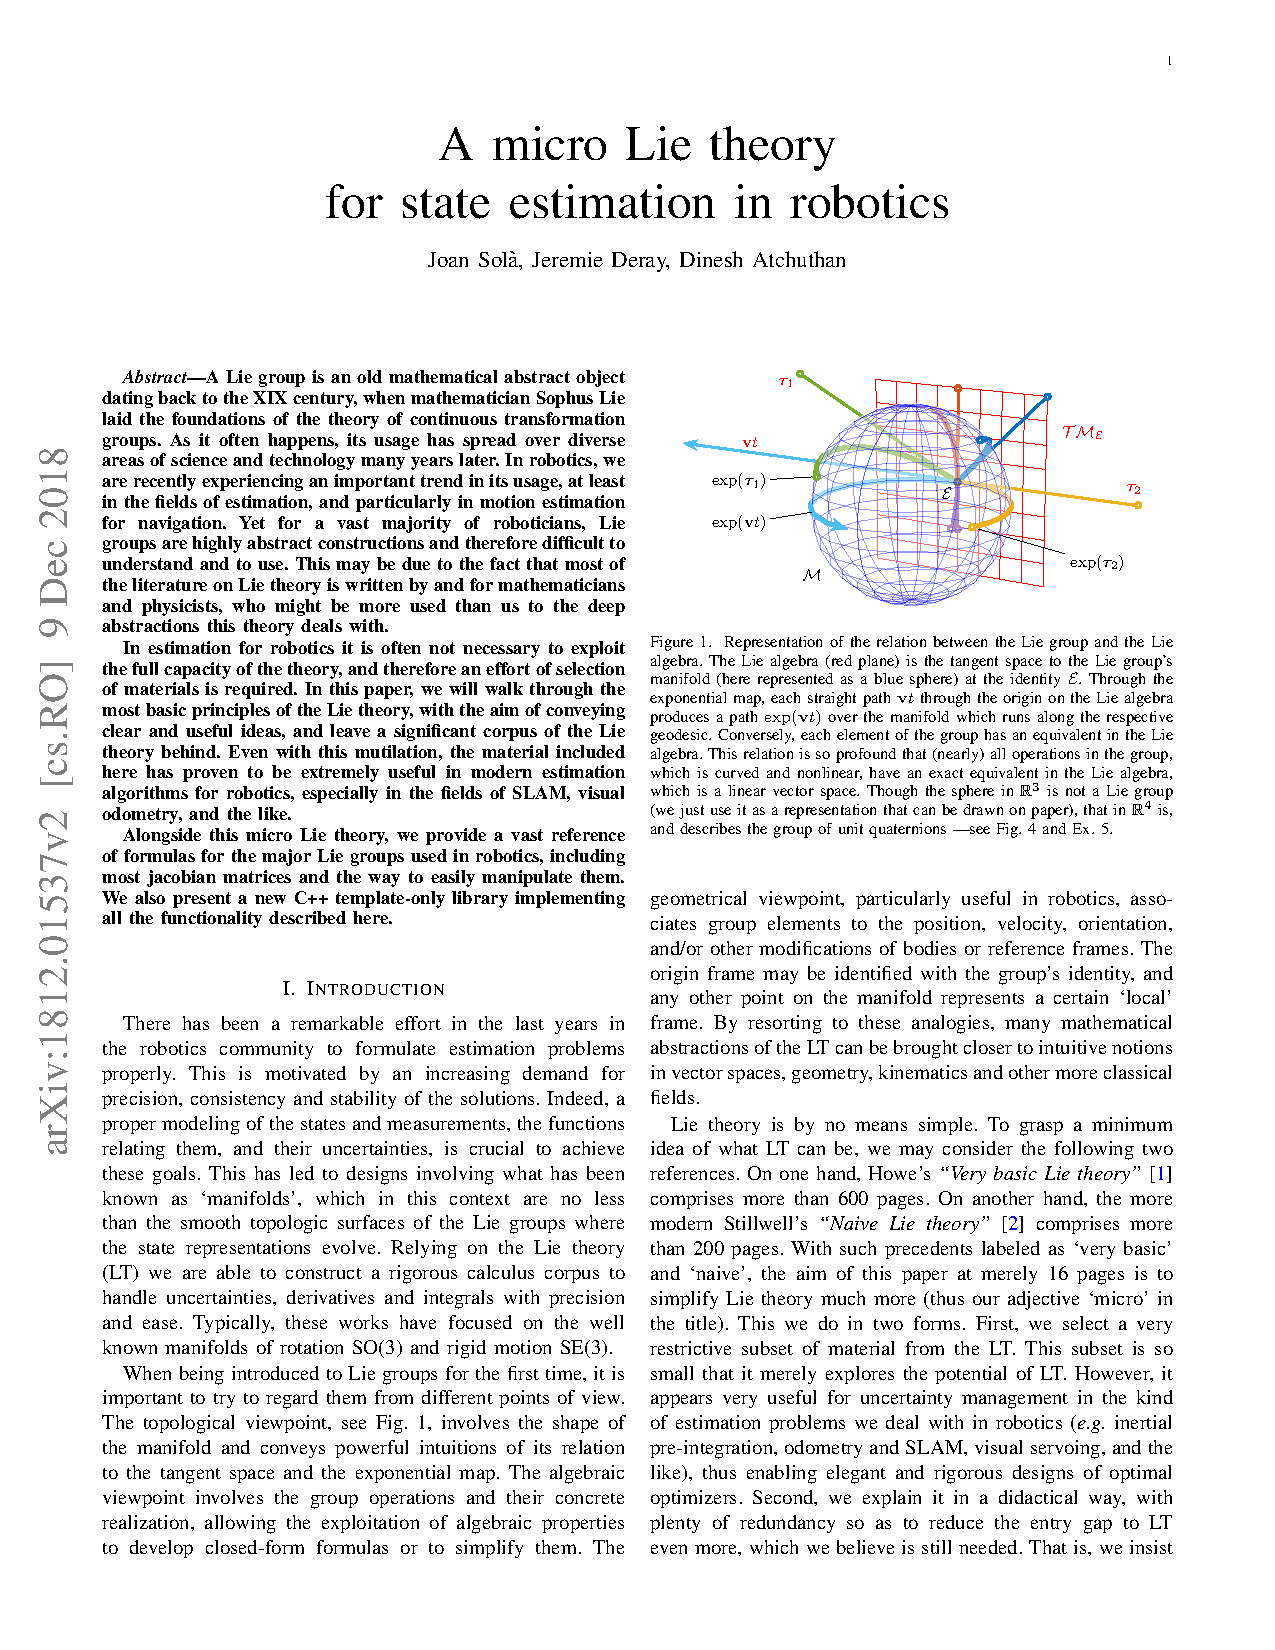
\includepdf[pages=-,scale=.8,pagecommand={}]{chap2_preliminaries/papers/micro_Lie_theory.pdf}




%!TEX root =../quadrotorbook.tex
\chapter{Multirotor Equations of Motion}
\label{chap:multirotor}

Author: Tim McLain, RWB

\section{Equations of Motion}
Let $\mathcal{F}_i$ denote an earth-fixed inertial reference frame with unit vectors $(\mathbf{i}_i,\mathbf{j}_i,\mathbf{k}_i)$ aligned with the north, east, and down directions. Let $\mathcal{F}_b$ denote a reference frame that is fixed with respect to the multirotor body having unit vectors $(\mathbf{i}_b,\mathbf{j}_b,\mathbf{k}_b)$ aligned with the forward, right, and down directions in the body frame. The orientation of the multirotor with respect to the inertial reference frame can be expressed by the rotation matrix $R_b^i \in \mathit{SO}(3)$ which can be expressed as\cite{BeardMcLain12}
\begin{equation}
R_b^i = 
\begin{pmatrix} c_{\theta} c_{\psi} & s_{\phi} s_{\theta} c_{\psi} - c_{\phi} s_{\psi}
& c_{\phi} s_{\theta} c_{\psi} + s_{\phi} s_{\psi} \\
c_{\theta} s_{\psi} &  s_{\phi} s_{\theta} s_{\psi} + c_{\phi} c_{\psi}
  & c_{\phi} s_{\theta} s_{\psi} - s_{\phi} c_{\psi}  \\
-s_{\theta} & s_{\phi} c_{\theta} & c_{\phi} c_{\theta}
\end{pmatrix},
\label{eq:eom_rot_1}
\end{equation}
where we have used the notation $c_x\defeq\cos x$ and $s_x\defeq \sin x$. The angles $(\phi,\theta,\psi)$ are the roll, pitch, and yaw Euler angles. The rotation matrix in equation~\eqref{eq:eom_rot_1} corresponds to the yaw-pitch-roll (3-2-1) rotation sequence.

We can represent the rigid-body dynamics of the multirotor with the equations of motion
\begin{align*}
	\dot{\mathbf{p}}_{b/i}^i &= \mathbf{v}_{b/i}^i \\
	\dot{\mathbf{v}}_{b/i}^i &= g \kbf_i^i + \frac{1}{m} R_b^i \mathbf{F}^b \\
	\dot{R}_b^i &= R_b^i \ss{\omegabf_{b/i}^b} \\
	J\dot{\omegabf}_{b/i}^b &= -\omegabf_{b/i}^b \times (\Jbf\omegabf_{b/i}^b) + \taubf^b.
\end{align*}
%
In these equations, $m$ denotes the mass of the multirotor and $\Jbf$ is the inertia matrix of the multirotor with respect to the body-frame axes. The vectors $\Fbf^b$ and $\taubf^b$ define the aerodynamic forces and moments experienced by the multirotor and are expressed in the body frame. The vectors $v_{b/i}^i$, $\omegabf_{b/i}^i$, and $p_{b/i}^i$ are the velocity, angular velocity, and position of the multirotor with respect to the inertial reference frame as expressed in the inertial frame, while the variable $g$ denotes the gravitational constant. The notation $\ss{\omegabf}$ represents the skew-symmetric matrix operator formed from the vector $\omegabf$ so that $\ss{\omegabf} \vbf = \omegabf \cross \vbf$ for the vector cross product $\cross$ and any vector $\vbf \in \mathbb{R}^3$.



%%%%%%%%%%%%%%%%% BEGIN OMIT
%
% This stuff is potentially useful. Just taking it out while we get main ideas in place
%
\OMIT{
In this chapter,  we derive expressions for the kinematics and the
dynamics of a rigid body.  While the expressions derived in this
chapter are general to any rigid body, we will use notation and
coordinate frames that are common in the aeronautics literature. In 
Section~\ref{sec:eom-state-variables}, we define the
notation that will be used for the state variables of a quadrotor.
In Section~\ref{sec:eom-kinematics} we derive expressions for
the kinematic equations of motion, and in Section~\ref{sec:eom-dynamics} we derive the
dynamic equations of motion from Newton's 2nd law.

\twmcomment{Later sections to introduce EOM using quaternions?}

\section{State Variables}
\label{sec:eom-state-variables}

\twmcomment{What is the generic name that we will use for the aircraft? Quadrotor doesn't seem right since we want to generalize to $N$ rotors. Multirotor seems fine, but it is a little long. What will our abbreviation be? MR? QR? MRA (for multirotor aircraft)? I think we should figure out what the mainstream folks are doing.}

State variables describe the energy state of the quadrotor as it flies about and include linear and angular positions, as well as linear and angular velocities. These state variables and their derivatives with respect to time represent the dynamic behavior of the quadrotor and are related to one another by ordinary differential equations that we call the equations of motion. A standard set of state variables for the quadrotor can be seen in table~\ref{tab:eom-state-varibles}. Some of the state variables are derived with respect to inertial reference frames, while others are derived with respect to reference frames fixed in the body of the quadrotor. We first introduce state variables and equations of motion that use Euler angles to represent the attitude of the quadrotor. In later sections we will express the attitude in terms of a quaternion representation along with the corresponding changes to the equations of motion..

The position of the quadrotor is represented with respect to a fixed (inertial) location on the earth using a north-east-down reference frame with the variables ($p_n$, $p_e$, $p_d$) as the position states. The attitude, or angular orientation, of the quadrotor is represented by the Euler angles ($\phi$, $\theta$, $\psi$), which are defined as described in section~\ref{sec:rotation_matrices}. The translational velocity of the quadrotor is represented by the variables ($u$, $v$, $w$), which are the components of the velocity vector in the directions of the body-frame ($\mathbf{i}^b$, $\mathbf{j}^b$, $\mathbf{k}^b$) axes of the quadrotor. The angular velocity of the quadrotor is represented by the variables ($p$, $q$, $r$), which are the components of the angular rates along these same body-frame axes. These state variables are depicted schematically in figure~\ref{fig:eom-state-variables}.
%
\begin{table}
\centering
\caption{State variables for MAV equations of motion.}
\label{tab:eom-state-variables}
\vspace{0.07in}
\begin{tabular}{|c|l|}
\hline
Name & Description \\
\hline \hline
$p_n$ & Inertial north position of quadrotor along $\mathbf{i}^i$ in $\mathcal{F}^i$.\\  \hline
$p_e$ & Inertial east position of quadrotor along $\mathbf{j}^i$ in $\mathcal{F}^i$.\\  \hline
$p_d$ & Inertial down position (negative of altitude) of quadrotor along $\mathbf{k}^i$ in $\mathcal{F}^i$.\\  \hline
$u$ & Body-frame velocity measured along $\mathbf{i}^b$ in $\mathcal{F}^b$.\\  \hline
$v$ & Body-frame velocity measured along $\mathbf{j}^b$ in $\mathcal{F}^b$.\\  \hline
$w$ & Body-frame velocity measured along $\mathbf{k}^b$ in $\mathcal{F}^b$.\\  \hline
$\phi$ & Roll angle defined with respect to $\mathcal{F}^{v2}$.\\  \hline
$\theta$ & Pitch angle defined with respect to $\mathcal{F}^{v1}$.\\  \hline
$\psi$ & Heading (yaw) angle defined with respect to $\mathcal{F}^v$. \\  \hline
$p$ & Roll rate measured along $\mathbf{i}^b$ in $\mathcal{F}^b$. \\  \hline
$q$ & Pitch rate measured along $\mathbf{j}^b$ in $\mathcal{F}^b$. \\  \hline
$r$ & Yaw rate measured along $\mathbf{k}^b$ in $\mathcal{F}^b$. \\
\hline
\end{tabular}
\end{table} \index{State Variables}
%
The body-frame axes of the quadrotor ($\mathbf{i}^b$, $\mathbf{j}^b$, $\mathbf{k}^b$) are commonly referred to as the roll, pitch, and yaw axes of the quadrotor respectively. The roll, pitch, and yaw rates ($p$, $q$, $r$) are measured about these axes. As explained in section~\ref{sec:frames-quadrotor-frames}, the Euler angles describing the yaw displacement $\psi$ and pitch displacement $\theta$ of the aircraft are defined by rotations about the $\mathbf{k}^{v}$ = $\mathbf{k}^{v1}$ and $\mathbf{j}^{v1}$ = $\mathbf{j}^{v2}$ axes that are not aligned with the body frame $\mathcal{F}^b$. Because of this, $\psi$ and $\theta$ cannot be expressed simply as rotations about the yaw and pitch axes of the aircraft. Furthermore, the pitch and yaw rates, $q$ and $r$, are not equivalent to the time derivatives of the pitch and yaw angles, $\theta$ and $\psi$. 
%
\begin{figure}[hhhhtb]
\begin{center}
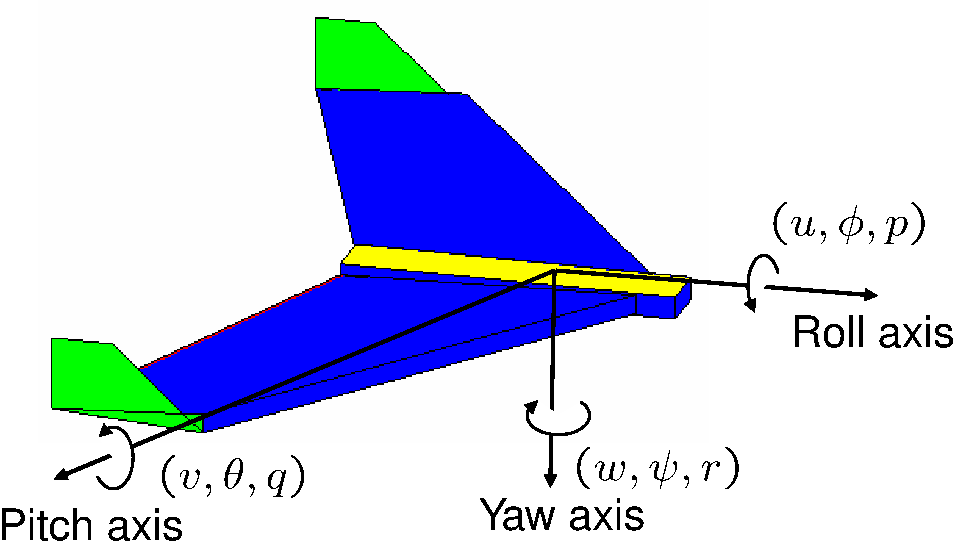
\includegraphics[width=3.5in]{chap3_multirotor/figures/kin-axis-definition}
\end{center}
\caption{Graphical definition of state variables.} \label{fig:eom-state-variables}
\end{figure}

\section{Kinematic Equations of Motion}
As we set out to derive equations of motion for the quadrotor, our goal is come up with relationships expressing derivatives of state variables in terms of state variables and inputs to the system. The kinematic equations describing the motion of the quadrotor, will involve relationships between derivatives of the position states and the velocity states without any consideration for the inputs to the system. In the sections that follow, we will first consider the translational kinematics, followed by the rotational kinematics.

\subsection{Translational Kinematics}
The translational kinematic equations of motion represent the relationship between the time derivatives of the position state variables ($\dot{p}_n$, $\dot{p}_e$, $\dot{p}_d$) that are defined with respect to a fixed inertial reference frame and the velocity state variables ($u$, $v$, $w$) that are defined with respect to the body frame of the quadrotor. Taking advantage of the rotational transformation between the body and vehicle (inertial) frame derived in equation~\eqref{eq:frames-Rvb}, the relationship between the translational positions and velocities is given by
\begin{equation*}
\frac{d}{dt} \begin{pmatrix} p_n \\ p_e \\ p_d \end{pmatrix} =
\mathcal{R}_{b}^{v} \begin{pmatrix} u \\ v \\ w \end{pmatrix}
= (\mathcal{R}_{v}^{b})^{\top} \begin{pmatrix} u \\ v \\ w \end{pmatrix} ,
\end{equation*}
which leads to
\begin{equation}
\begin{pmatrix} \dot{p}_n \\ \dot{p}_e \\ \dot{p}_d \end{pmatrix} = \begin{pmatrix} c_{\theta} c_{\psi} & s_{\phi} s_{\theta} c_{\psi} - c_{\phi} s_{\psi}
& c_{\phi} s_{\theta} c_{\psi} + s_{\phi} s_{\psi} \\
c_{\theta} s_{\psi} &  s_{\phi} s_{\theta} s_{\psi} + c_{\phi} c_{\psi}
  & c_{\phi} s_{\theta} s_{\psi} - s_{\phi} c_{\psi}  \\
-s_{\theta} & s_{\phi} c_{\theta} & c_{\phi} c_{\theta}
\end{pmatrix}
\begin{pmatrix} u \\ v \\ w \end{pmatrix},
\label{eq:kin-trans-1}
\end{equation}
where we have used the notation $c_x\defeq\cos x$ and $s_x\defeq \sin x$. These equations represent three of the 12 state equations that we will define.

\subsection{Rotational Kinematics} 
The rotational kinematic equations of motion relate the time derivatives of the Euler angles ($\dot{\phi}$, $\dot{\theta}$, $\dot{\psi}$) and the body-frame angular rates ($p$, $q$, $r$). While the angular motion represented by $\dot{\phi}$ can be thought of as a rotation about the body-frame $\mathbf{i}^b$ axis, the motions represented by $\dot{\theta}$ and $\dot{\psi}$ are not defined as rotations about unique body axes. Instead, they are defined in section~\ref{sec:rotation_matrices} as rotations about the intermediate axes $\mathbf{j}^{v2}$ and $\mathbf{k}^{v1}$ respectively. We can relate these Euler angle derivatives to the body-fixed angular rates by rotating the Euler angle derivatives into the body-fixed reference frame and summing them to give
\begin{align}
\begin{pmatrix} p \\ q \\ r \end{pmatrix} &=
\begin{pmatrix} \dot{\phi} \\ 0 \\ 0
\end{pmatrix}
+ \mathcal{R}_{v2}^{b}(\phi) \begin{pmatrix} 0 \\ \dot{\theta} \\
0 \end{pmatrix} + \mathcal{R}_{v2}^{b}(\phi) \mathcal{R}_{v1}^{v2}(\theta)
    \begin{pmatrix} 0 \\ 0 \\ \dot{\psi} \end{pmatrix}  \notag \\
&= \begin{pmatrix} \dot{\phi} \\ 0 \\ 0 \end{pmatrix}
+ \begin{pmatrix}
    1 & 0 & 0 \\
    0 & c_{\phi} & s_{\phi} \\
    0 & -s_{\phi} & c_{\phi}
  \end{pmatrix}
  \begin{pmatrix} 0 \\ \dot{\theta} \\ 0 \end{pmatrix}
+ \begin{pmatrix}
    1 & 0 & 0 \\
    0 & c_{\phi} & s_{\phi} \\
    0 & -s_{\phi} & c_{\phi}
  \end{pmatrix}
  \begin{pmatrix}
    c_{\theta} & 0 & -s_{\theta} \\
    0 & 1 & 0 \\
    s_{\theta} & 0 & c_{\theta}
  \end{pmatrix}
  \begin{pmatrix} 0 \\ 0 \\ \dot{\psi} \end{pmatrix}  \notag \\
&= \begin{pmatrix}
  1 & 0 & -s_{\theta} \\
  0 & c_{\phi} & s_{\phi} c_{\theta} \\
  0 & -s_{\phi} & c_{\phi} c_{\theta}
\end{pmatrix}
\begin{pmatrix} \dot{\phi} \\ \dot{\theta} \\ \dot{\psi} \end{pmatrix}.
\label{eq:kin-phithetapsidot-to-pqr}
\end{align}
Inverting this expression leads to the rotational kinematic equations of motion\index{Kinematics!Rotation}
\begin{equation} \label{eq:kin-rotational-kinematics}
\begin{pmatrix} \dot{\phi} \\ \dot{\theta} \\ \dot{\psi} \end{pmatrix}
= \begin{pmatrix}
  1 & \sin\phi\tan\theta & \cos\phi\tan\theta \\
  0 & \cos\phi & -\sin\phi \\
  0 & \sin\phi\sec\theta & \cos\phi\sec\theta
  \end{pmatrix}
  \begin{pmatrix} p \\ q \\ r \end{pmatrix} ,
\end{equation}
%
These equations express the derivatives of the three angular position states in terms of
the angular positions $\phi$ and $\theta$ and the body angular rates $p$, $q$, and $r$.

\twmcomment{I included the angular stuff for my own benefit. Once we have chapters 2 and 3 laid out, we can decide what goes where. I'd like to understand the new formulations of the EOM, so I will probably write about them to learn -- not trying to dictate what goes where.}

\twmcomment{START HERE!!!}

\section{Dynamic Equations of Motion}

- Do both translational and rotational dynamics

\subsection{Gravity Force}

}
%%%%%%%%%% END OMIT

%%%% Start here -- integrate induced drag into discussion

\subsection{Rotor Forces and Torques}
The aerodynamic forces and torques that enable the agile flight of a multirotor come from the dc-motor/propeller modules that we call the rotors. In hover, the rotors of a multirotor each provide a constant and equal thrust to overcome the effects of gravity. The rotors of a multirotor are usually configured in counter-rotating pairs, one rotating clockwise and the other counter-clockwise, so that the motor torques acting on the multirotor cancel out  when in a non-rotating hover state. As the rotors rotate, the drag on the propellers produce a torque on the body of the aircraft opposite to the direction of rotation. Figure~\ref{fig:eom-octo-std-def} depicts an octocopter with equally spaced counter-rotating rotors as an example of how a multirotor can be configured.

% Give marginfigures a try
\begin{marginfigure}
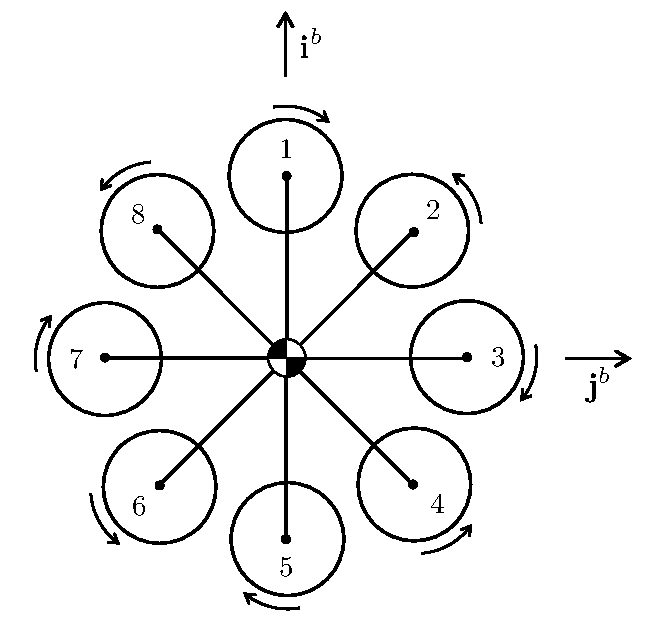
\includegraphics{chap3_multirotor/figures/eom-octo-std-def}
\caption{Octocopter example of a multirotor configuration.} 
\label{fig:eom-octo-std-def}
\end{marginfigure}
%

To accelerate the multirotor up or down, the speed of the rotors can be uniformly increased or decreased away from their nominal speed. To pitch up or down about the $\mathbf{j}_b$ axis, the speed differential between the fore and aft rotors can be sped up or slowed down. Similarly, to roll the aircraft right or left about the $\mathbf{i}_b$ axis the speed differential between the left and right rotors can be varied. To yaw the aircraft about the $\mathbf{k}_b$ axis, on the other hand, the speed differential between the clockwise-rotating props and counter-clockwise-rotating props is varied.

In modeling the aerodynamic forces and torques acting on the multirotor, we will consider thrust force $F_\text{thrust}$, the drag force $F_\text{drag}$, and the torque produced by the rotors. In this section, we will develop the relationship between the thrust force $F_{\text{thrust}}$, the roll, pitch, and yaw torques ($\tau_x$, $\tau_y$, $\tau_z$) and the individual rotor angular speeds. For an $N$-rotor aircraft, these angular speeds will be given by ($\omega_1$, $\omega_2$, $\ldots$, $\omega_N$) and specified in radians per second. From propeller theory, the thrust and torque produced by a single rotor in hover can be modeled as
\begin{align}
	T_i &= C_T \frac{\rho D^4}{4\pi^2} \omega_i^2	\\
	Q_i &= C_Q \frac{\rho D^5}{4\pi^2} \omega_i^2,	
\end{align}
where $\rho$ is the density of air, $D$ is the propeller diameter, and $C_T$ and $C_Q$ are non-dimensional aerodynamic coefficients specific to the propeller. 




The total rotor thrust for the multirotor is given by
\begin{equation}
   F_{\text{thrust}} = \sum\limits_{i=1}^N T_i ,
\end{equation}
where $F_i$ is the thrust force produced by rotor $i$.

%The negative sign takes into account that the thrust force is up in the body frame of the aircraft, while we have defined $F_z$ as positive down in the body frame. 

To define the torques produced by the rotors, we need to define the configuration of each rotor relative to the center of mass of the aircraft and its direction of rotation. Figure~\ref{fig:eom-rotor-definition} highlights a single rotor $i$ for an arbitrary multirotor configuration. The variable $\varphi_i$ is the angle between the forward direction of the multirotor, defined by the unit vector $\mathbf{i}^b$, and the radial direction of the $i^{\mathit{th}}$ rotor. The variable $\ell_i$ represents the radial distance from the center of mass to the $i^{\mathit{th}}$ rotor. The variable $d_i$ indicates the direction of rotation for each rotor as
%
%
\begin{marginfigure}
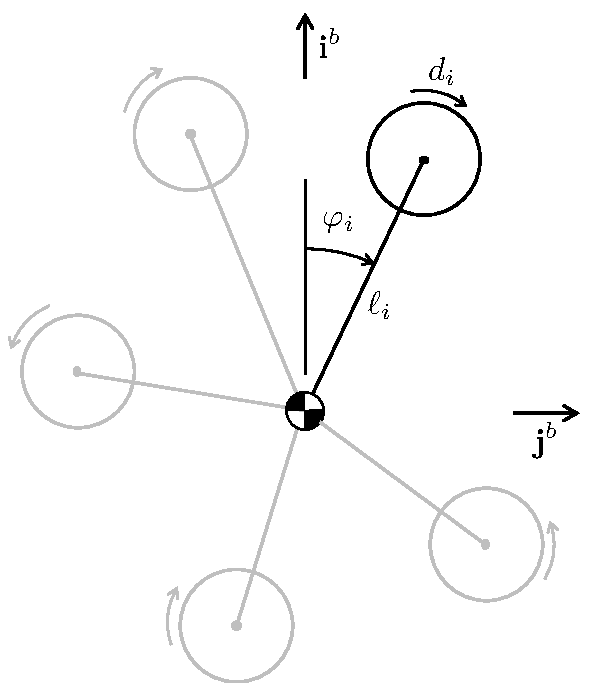
\includegraphics{chap3_multirotor/figures/eom-rotor-definition}
\caption{Definition of rotor configuration variables.} 
\label{fig:eom-rotor-definition}
\end{marginfigure}
%
%
\begin{equation}
   d_i = 
   \begin{cases}
      -1 	& \text{for CW rotation} \\
      +1 	& \text{for CCW rotation} .
   \end{cases}
\end{equation}
%
From the configuration geometry of Figure~\ref{fig:eom-rotor-definition}, the total roll torque about the $\mathbf{i}_b$ axis is given by
\begin{equation}
   \tau_x = - \sum\limits_{i=1}^N \left( \ell_i \sin \varphi_i \right) T_i .
\end{equation}
Similarly, the total pitch torque about the $\mathbf{j}_b$ axis can be calculated as
\begin{equation}
   \tau_y = \sum\limits_{i=1}^N \left( \ell_i \cos \varphi_i \right) T_i .
\end{equation}
Finally, the total yaw torque about the $\mathbf{k}_b$ axis, which depends on the direction of rotation of each rotor, is given by
\begin{equation}
   \tau_z = \sum\limits_{i=1}^N d_i Q_i .
\end{equation}
%
%
%\begin{marginfigure}
%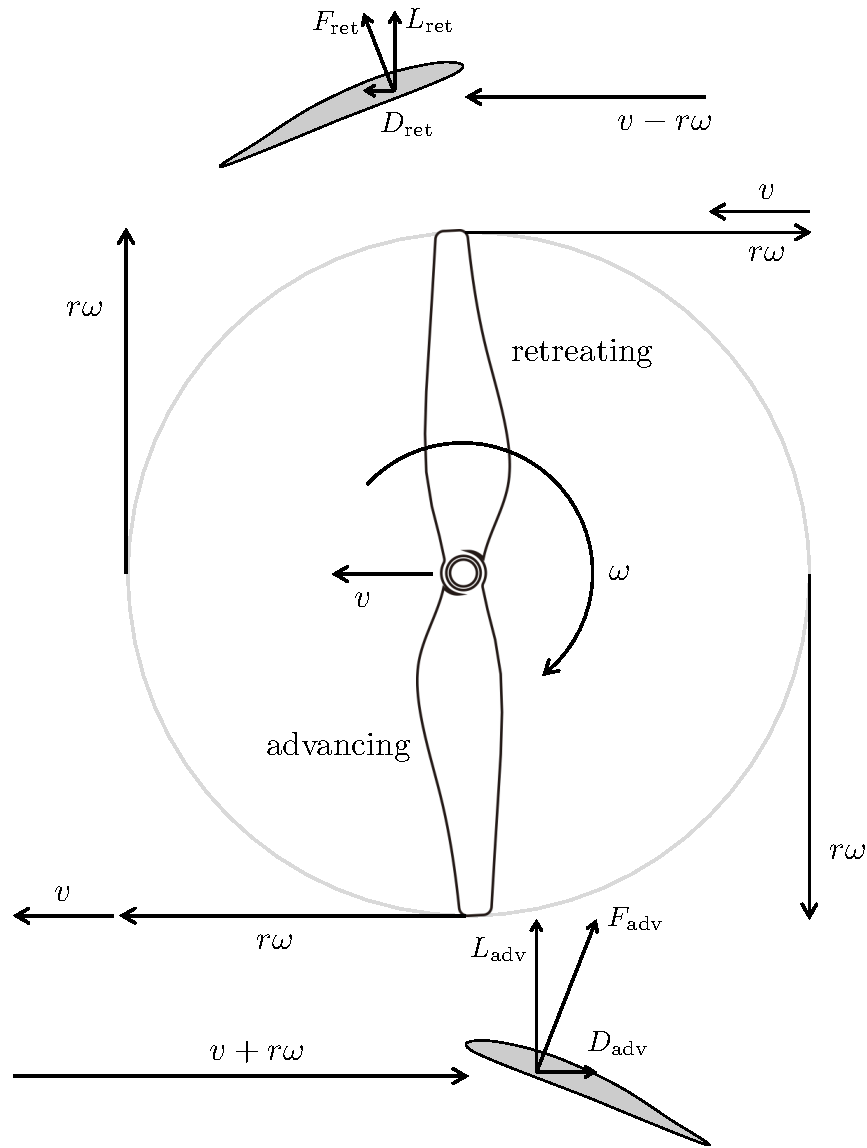
\includegraphics{chap3_multirotor/figures/eom-induced-drag}
%\caption{Induced rotor drag concept.} 
%\label{fig:eom-induced-drag}
%\end{marginfigure}
%
%

As with any lifting surface, induced drag forces are generated from the lift forces created by the rotating propellers. The direction of the drag force on a propeller blade at any instant is in the direction opposite of the velocity of the blade tip. Since the blade tip is moving much faster than the airspeed of the multirotor motion. When the blade is advancing into the oncoming apparent wind generated by the combination of multirotor motion and the wind, the induced drag is higher than when the blade is in the retreating portion of its circular motion and moving with the apparent wind. The net effect is that each of the rotors on the aircraft creates an induced drag force that is in the plane of the rotor and proportional to the projection of the lift force onto the plane of the rotor in magnitude and directed opposite to the airspeed vector. 
%
\begin{figure}[hhhhtb]
\begin{center}
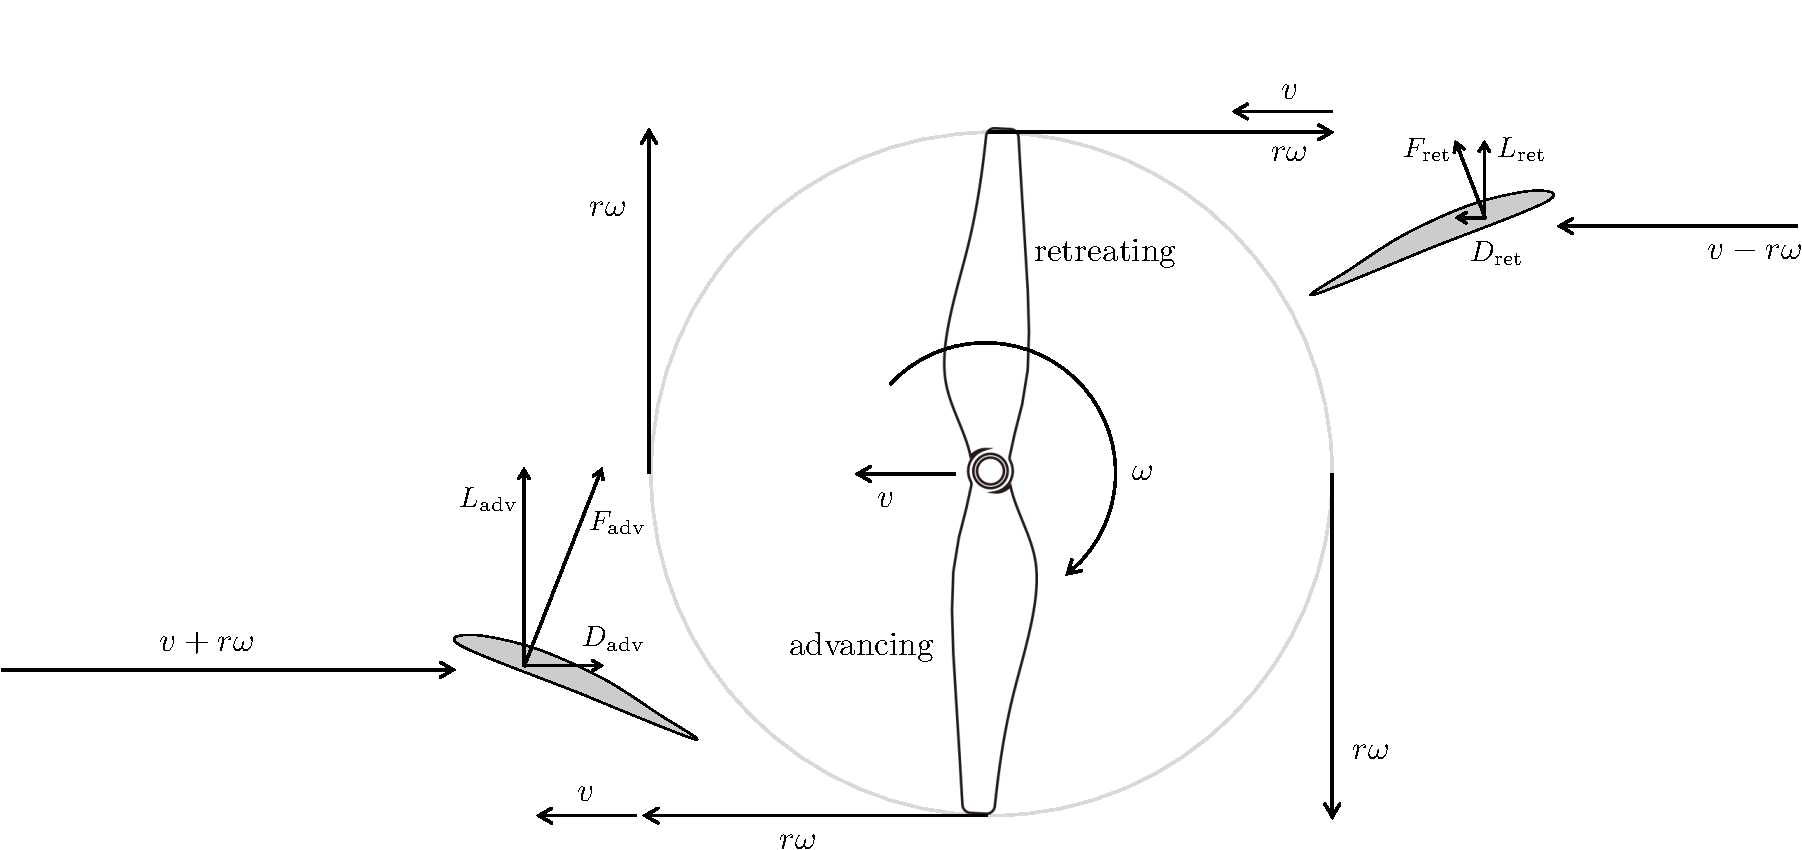
\includegraphics[width=6.5in]{chap3_multirotor/figures/eom-induced-drag2}
\end{center}
\caption{Induced drag.} \label{fig:eom-induced-drag}
\end{figure}
%
%
The drag force is also proportional to the component of the airspeed in the rotor plane.\cite{MahonyKC12} Accordingly, the drag force can be represented as 
\begin{align*}
	\Fbf_\text{drag}^b &\approx - F_\text{thrust} C_d \; \text{diag}(1,1,0) \vbf_{b/i}^b \\
	&= \begin{pmatrix} F_\text{thrust}C_d & 0 & 0 \\ 0 & F_\text{thrust}C_d & 0 \\ 0 & 0 & 0 \end{pmatrix}\vbf_{b/i}^b.
\end{align*}
Since the thrust force is approximately equal to $mg$, the weight of the aircraft, we can define
\[
D = \begin{pmatrix} gC_d & 0 & 0 \\ 0 & gC_d & 0 \\ 0 & 0 & 0 \end{pmatrix}
\]
and write induced drag in the body frame as
\begin{align*}
	\Fbf_\text{drag}^b &\approx mD R_b^{i\top} \vbf_{b/i}^i.	\label{eq:induced drag}
\end{align*}
In the following we write the thrust force as
\[
F_{\text{thrust}} = mT,
\]
where $T$ is the throttle setting.  
%
Therefore, the total aerodynamic force in the body frame is approximated as
\begin{align}
	\Fbf^b &\approx - mT \kbf_b^b + mD R_b^{i\top} \vbf_{b/i}^i.
\end{align}
In the inertial frame, the aerodynamic force is \sidenote{Recall that $\kbf_b^b = \ebf_3 = (0, 0, 1)^\top$}.
\begin{align}
	\Fbf^i &\approx - m T \ebf_3 + m R D R_b^{i\top} \vbf_{b/i}^i.
\end{align}


\section{Multirotor Mass Properties}
The mass properties of multirotors of particular interest to us are its mass $m$, center of mass location, and its inertia matrix $\Jbf$. The mass of a multirotor is distributed over the aircraft and the inertia matrix models how the mass is distributed and its effect on the rotational dynamics of the aircraft. Because the distribution of the mass of the aircraft is fixed in the body frame, $\Jbf$ is constant with respect to the body axes $(\ibf_b, \jbf_b, \kbf_b)$ and can be calculated as
\begin{align*}
\mathbf{J} &=
    \begin{pmatrix}
    \int (y^2 + z^2)\,dm & -\int xy\,dm         & -\int xz\,dm \\
    -\int xy\,dm         & \int (x^2 + z^2)\,dm &  -\int yz\,dm \\
    -\int xz\,dm         & -\int yz\,dm         & \int (x^2 + y^2)\,dm
    \end{pmatrix} \\
&\defeq
    \begin{pmatrix}
    J_{x}   & -J_{xy} & -J_{xz} \\
    -J_{xy} & J_{y}   & -J_{yz} \\
    -J_{xz} & -J_{yz} & J_{z}
    \end{pmatrix} .
\end{align*}

The diagonal terms of $\Jbf$ are called the moments of inertia and the off-diagonal terms are called the products of inertia. Multirotor aircraft tend to be symmetric in their shape and mass distribution and this results in significant simplification in the inertia matrix. In particular, if the aircraft is symmetric with respect to the $\ibf_b$-$\jbf$, $\ibf_b$-$\kbf$, and $\jbf_b$-$\kbf$ planes, then the products of inertia, $J_{xy}$, $J_{xz}$, and $J_{yz}=0$, are zero resulting in
\[
\mathbf{J} =
    \begin{pmatrix}
    J_{x}   & 0       & 0 \\
    0       & J_{y}   & 0 \\
    0 & 0       & J_{z}
    \end{pmatrix}.
\]
%
\begin{marginfigure}
	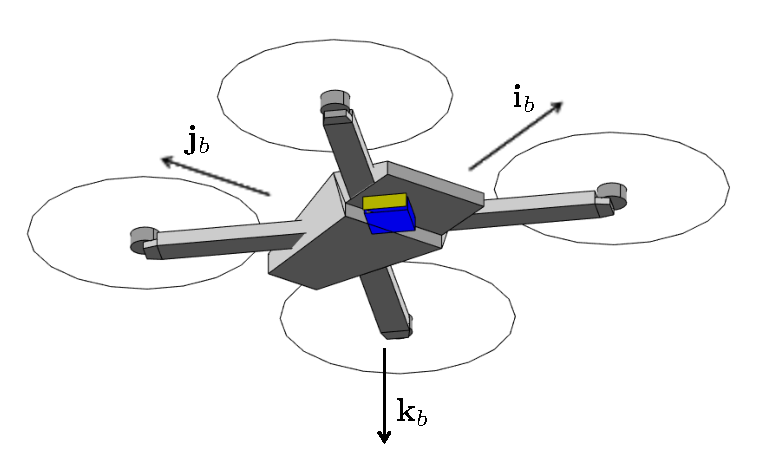
\includegraphics{chap3_multirotor/figures/eom-quad-axes}
	\caption{Quadrotor with body-frame axes that coincide at the center of mass.}
	\label{fig:eom-quad-axes}
\end{marginfigure}
%
Importantly, under these symmetry conditions, $\Jbf$ is easily inverted with its inverse expressed as
\begin{align*}
\mathbf{J}^{-1}
    &= \begin{pmatrix}
        \frac{1}{J_x} & 0 & 0 \\
        0 & \frac{1}{J_y} & 0 \\
        0 & 0 & \frac{1}{J_z}
       \end{pmatrix} .
\end{align*}

If a high-quality CAD model is available, the moments and products of inertia and the center of mass location can commonly be calculated numerically using the CAD software. Alternatively, moments of inertia and the center of mass location can be measured experimentally using equipment such as a bifilar pendulum. For simple geometries, the moments of inertia and center of mass can be calculated from moments of inertia of basic shapes and the parallel axis theorem. For example, the moments of inertia for the quadrotor shown in Figure~\ref{fig:eom-quad-axes} can be calculated by assuming that the quadrotor body is approximated by a cuboid with a specific length, width, mass, and uniform density. The rotor motors, arms, and propellers can be approximated as point masses located at the motor positions.

Summarizing, the equations of motion for the multirotor are given by
\begin{align}
	\dot{\pbf}_{b/i}^i &= \vbf_{b/i}^i \label{eq:eom_p} \\
	\dot{\vbf}_{b/i}^i &= g \ebf_3 - TR_b^i \ebf_3 + R_b^i D R_b^{i\top} \vbf_{b/i}^i  \label{eq:eom_v} \\
	\dot{R}_b^i &= R_b^i \ss{\omegabf_{b/i}^b} \label{eq:eom_R} \\
	J\dot{\omegabf}_{b/i}^b &= -\omegabf_{b/i}^b \times (J\omegabf_{b/i}^b) + \taubf^b. \label{eq:eom_omega}
\end{align}



%%%%%%%%%%%%%%%%%%%% Begin BIG omit
\OMIT{
%
%\begin{figure}[hhhhtb]
%\begin{center}
%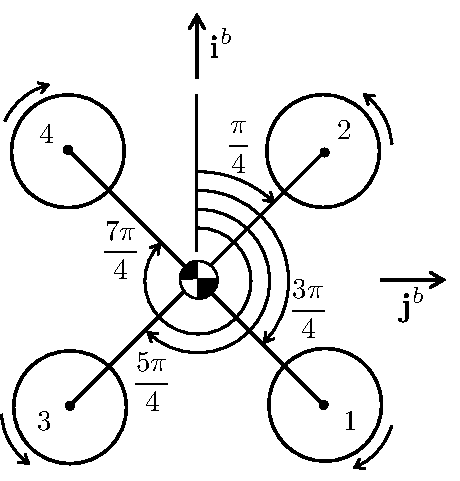
\includegraphics[width=3.0in]{chap3_multirotor/figures/eom-CF-quadX}
%\end{center}
%\caption{Definition of rotor variables for Cleanflight Quad X configuration.} \label{fig:eom-CF-quadX}
%\end{figure}
%

%
%\begin{figure}[hhhhtb]
%\begin{center}
%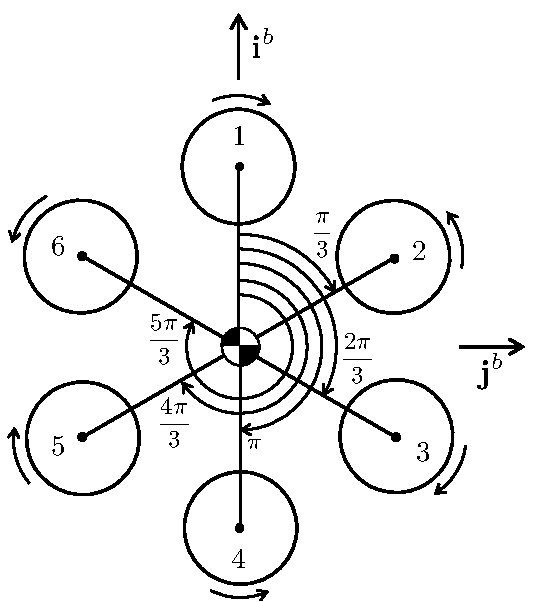
\includegraphics[width=3.0in]{chap3_multirotor/figures/eom-CF-hexa-plus}
%\end{center}
%\caption{Definition of rotor variables for Cleanflight Hexa Plus configuration.} \label{fig:eom-CF-hexa-plus}
%\end{figure}
%

%
%\begin{figure}[hhhhtb]
%\begin{center}
%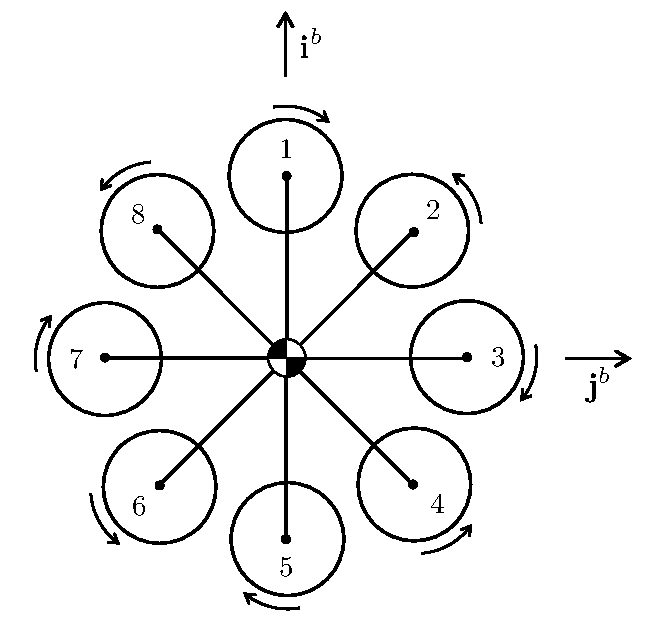
\includegraphics[width=3.5in]{chap3_multirotor/figures/eom-octo-std-def}
%\end{center}
%\caption{Recommended standard for rotor configuration variables.} \label{fig:eom-octo-std-def}
%\end{figure}
%


%- discuss the forces and moments due to different rotor configurations.   Make this part as general as possible to show how a variety of configurations can be handled.
%
%- Discussion of rotor drag term in translational dynamics
%
%- Rotor model (could get Andrew Ning to help out here)

\section{Body Frame Equations of Motion}

- Body relative equations of motion.  Provide some motivation for this model.

\section{Simplified Equations of Motion}

Show how certain assumptions lead to simplified equations of motion

- Euler angle models when roll and pitch angles are small

- equations of motion relative to a target, etc.


\section{Old stuff that might be useful}


%\chapter{Mathematical Preliminaries}
\section{Kinematics and Dynamics} \label{chap:kinematics}

In this chapter we derive the expressions for the kinematics and the
dynamics of a rigid body.  While the expressions derived in this
chapter are general to any rigid body, we will use notation and
coordinate frames that are typical in the aeronautics literature. In
particular, in Section~\ref{sec:kin-state-variables} we define the
notation that will be used for the state variables of a quadrotor.
In Section~\ref{sec:kin-kinematics} we derive the expressions for
the kinematics, and in Section~\ref{sec:kin-dynamics} we derive the
dynamics.



%%+++++++++++++++++++
\subsection{Quadrotor State Variables} %
\label{sec:kin-state-variables}

The state variables of the quadrotor are the following twelve
quantities
\begin{align*}
p_n &= \text{~the inertial (north) position of the quadrotor along $\hat{i}^i$ in $\mathcal{F}^i$,}\\
p_e &= \text{~the inertial (east) position of the quadrotor along $\hat{j}^i$ in $\mathcal{F}^i$,}\\
h &= \text{~the altitude of the aircraft measured along $-\hat{k}^i$ in $\mathcal{F}^i$,}\\
u &= \text{~the body frame velocity measured along $\hat{i}^b$ in $\mathcal{F}^b$,}\\
v &= \text{~the body frame velocity measured along $\hat{j}^b$ in $\mathcal{F}^b$,}\\
w &= \text{~the body frame velocity measured along $\hat{k}^b$ in $\mathcal{F}^b$,}\\
\phi &= \text{~the roll angle defined with respect to $\mathcal{F}^{v2}$,}\\
\theta &= \text{~the pitch angle defined with respect to $\mathcal{F}^{v1}$,}\\
\psi &= \text{~the yaw angle defined with respect to $\mathcal{F}^v$,} \\
p &= \text{~the roll rate measured along $\hat{i}^b$ in $\mathcal{F}^b$,}\\
q &= \text{~the pitch rate measured along $\hat{j}^b$ in $\mathcal{F}^b$,} \\
r &= \text{~the yaw rate measured along $\hat{k}^b$ in
$\mathcal{F}^b$.}
\end{align*}
The state variables are shown schematically in
Figure~\ref{fig:kin-axis-definition}.
%
\begin{figure}[hhhhtb]
\begin{center}
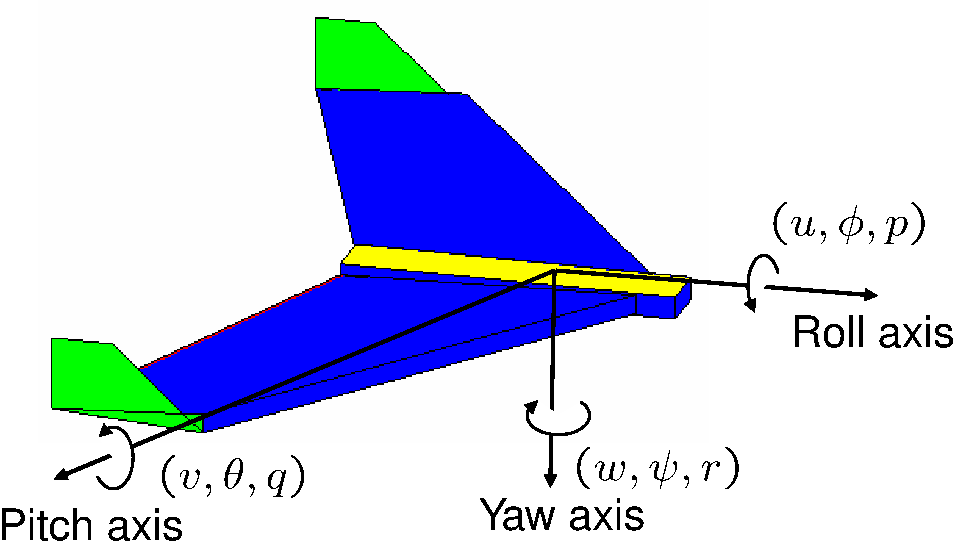
\includegraphics[width=3.0in]{chap3_multirotor/figures/kin-axis-definition}
\end{center}
\caption{Definition of Axes} \label{fig:kin-axis-definition}
\end{figure}
%
The position $(p_n, p_e, h)$ of the quadrotor is given in the
inertial frame, with positive $h$ defined along the negative $Z$
axis in the inertial frame.  The velocity $(u,v,w)$ and the angular
velocity $(p,q,r)$ of the quadrotor are given with respect to the
body frame.  The Euler angles (roll $\phi$, pitch $\theta$, and yaw
$\chi$) are given with respect to the vehicle 2-frame, the vehicle
1-frame, and the vehicle frame respectively.





%%+++++++++++++++++++
\subsection{Quadrotor Kinematics} %
\label{sec:kin-kinematics}

The state variables $p_n$, $p_e$, and $-h$ are inertial frame
quantities, whereas the velocities $u$, $v$, and $w$ are body frame
quantities. Therefore the relationship between position and
velocities is given by
\begin{align*}
\frac{d}{dt} \begin{pmatrix} p_n \\ p_e \\ -h \end{pmatrix} &=
R_{b}^{v} \begin{pmatrix} u \\ v \\ w \end{pmatrix} \\
&= (R_{v}^{b})^T \begin{pmatrix} u \\ v \\ w \end{pmatrix} \\
&= \begin{pmatrix} c\theta c\psi & s\phi s\theta c\psi - c\phi s\psi
& c\phi s\theta
c\psi + s\phi s\psi \\
c\theta s\psi &  s\phi s\theta s\psi + c\phi c\psi
  & c\phi s\theta s\psi - s\phi c\psi  \\
-s\theta & s\phi c\theta & c\phi c\theta
\end{pmatrix}
\begin{pmatrix} u \\ v \\ w \end{pmatrix}.
\end{align*}


The relationship between absolute angles $\phi$, $\theta$, and
$\psi$, and the angular rates $p$, $q$, and $r$ is also complicated
by the fact that these quantities are defined in different
coordinate frames.  The angular rates are defined in the body frame
$\mathcal{F}^b$, whereas the roll angle $\phi$ is defined in
$\mathcal{F}^{v2}$, the pitch angle $\theta$ is defined in
$\mathcal{F}_{v1}$, and the yaw angle $\psi$ is defined in the
vehicle frame $\mathcal{F}^{v}$.

We need to relate $p$, $q$, and $r$ to $\dot{\phi}$, $\dot{\theta}$,
and $\dot{\psi}$.  Since $\dot{\phi}$, $\dot{\theta}$, $\dot{\psi}$
are small and noting that
\[
R_{v2}^{b}(\dot{\phi}) = R_{v1}^{v2}(\dot{\theta}) =
R_{v}^{v1}(\dot{\psi}) = I,
\]
we get
\begin{align}
\begin{pmatrix} p \\ q \\ r \end{pmatrix} &=
R_{v2}^{b}(\dot{\phi}) \begin{pmatrix} \dot{\phi} \\ 0 \\ 0
\end{pmatrix}
+ R_{v2}^{b}(\phi)R_{v1}^{v2}(\dot{\theta}) \begin{pmatrix} 0 \\ \dot{\theta} \\
0 \end{pmatrix} + R_{v2}^{b}(\phi) R_{v1}^{v2}(\theta) R_{v\to
v1}(\dot{\psi})
    \begin{pmatrix} 0 \\ 0 \\ \dot{\psi} \end{pmatrix}  \notag \\
&= \begin{pmatrix} \dot{\phi} \\ 0 \\ 0 \end{pmatrix} +
\begin{pmatrix}
    1 & 0 & 0 \\
    0 & \cos\phi & \sin\phi \\
    0 & -\sin\phi & \cos\phi
  \end{pmatrix}
  \begin{pmatrix} 0 \\ \dot{\theta} \\ 0 \end{pmatrix}
+ \begin{pmatrix}
    1 & 0 & 0 \\
    0 & \cos\phi & \sin\phi \\
    0 & -\sin\phi & \cos\phi
  \end{pmatrix}
  \begin{pmatrix}
    \cos\theta & 0 & -\sin\theta \\
    0 & 1 & 0 \\
    \sin\theta & 0 & \cos\theta
  \end{pmatrix}
  \begin{pmatrix} 0 \\ 0 \\ \dot{\psi} \end{pmatrix}  \notag \\
&= \begin{pmatrix}
  1 & 0 & -s\theta \\
  0 & c\phi & s\phi c\theta \\
  0 & -s\phi & c\phi c\theta
\end{pmatrix}
\begin{pmatrix} \dot{\phi} \\ \dot{\theta} \\ \dot{\psi} \end{pmatrix}.
\label{eq:kin-phithetapsidot-to-pqr}
\end{align}
Inverting we get
\begin{equation} \label{eq:kin-rotational-kinematics}
\begin{pmatrix} \dot{\phi} \\ \dot{\theta} \\ \dot{\psi} \end{pmatrix}
= \begin{pmatrix}
  1 & \sin(\phi)\tan(\theta) & \cos(\phi)\tan(\theta) \\
  0 & \cos(\phi) & -\sin(\phi) \\
  0 & \sin(\phi)\sec(\theta) & \cos(\phi)\sec(\theta)
  \end{pmatrix}
  \begin{pmatrix} p \\ q \\ r \end{pmatrix}.
\end{equation}

%%+++++++++++++++++++
\subsection{Rigid Body Dynamics} %
\label{sec:kin-dynamics}

Let $\mathbf{v}$ be the velocity vector of the quadrotor. Newton's
laws only hold in inertial frames, therefore Newton's law applied to
the translational motion is
\[
m \frac{d\mathbf{v}}{dt_i} =  \mathbf{f},
\]
where $m$ is the mass of the quadrotor, $\mathbf{f}$ is the total
applied to the quadrotor, and $\frac{d}{dt_i}$ is the time
derivative in the inertial frame.  From the equation of Coriolis we
have
\begin{equation} \label{eq:newton_translation}
m \frac{d\mathbf{v}}{dt_i}
    = m \left(
        \frac{d\mathbf{v}}{dt_b} + \boldsymbol{\omega}_{b/i}\times\mathbf{v}
         \right) = \mathbf{f},
\end{equation}
where $\boldsymbol{\omega}_{b/i}$ is the angular velocity of the
airframe with respect to the inertial frame.  Since the control
force is computed and applied in the body coordinate system, and
since $\boldsymbol{\omega}$ is measured in body coordinates, we will
express Eq~\eqref{eq:newton_translation} in body coordinates, where
$\mathbf{v}^b \defeq (u, v, w)^T$, and $\omega^b_{b/i} \defeq (p, q,
r)^T$.  Therefore, in body coordinates,
Eq.~\eqref{eq:newton_translation} becomes
\begin{equation} \label{eq:kin-translational-dynamics}
\begin{pmatrix} \dot{u} \\ \dot{v} \\ \dot{w} \end{pmatrix}
= \begin{pmatrix} rv-qw \\ pw-ru \\ qu-pv \end{pmatrix} +
\frac{1}{m} \begin{pmatrix} f_x \\ f_y \\ f_z \end{pmatrix},
\end{equation}
where $\mathbf{f}^b \defeq (f_x,  f_y, f_z)^T$.

For rotational motion, Newton's second law states that
\[
\frac{d\mathbf{h}^b}{dt_i} = \mathbf{m},
\]
where $\mathbf{h}$ is the angular momentum and $\mathbf{m}$ is the
applied torque.  Using the equation of Coriolis we have
\begin{equation}\label{eq:newton_rotation}
\frac{d\mathbf{h}}{dt_i} = \frac{d\mathbf{h}}{dt_b} +
\boldsymbol{\omega}_{b/i}\times\mathbf{h}  = \mathbf{m}.
\end{equation}
Again, Eq.~\eqref{eq:newton_rotation} is most easily resolved in
body coordinates where $\mathbf{h}^b =
\mathbf{J}\boldsymbol{\omega^b_{b/i}}$ where $\mathbf{J}$ is the
constant inertia matrix given by
\begin{align*}
\mathbf{J} &=
    \begin{pmatrix}
    \int (y^2 + z^2)\,dm & -\int xy\,dm         & -\int xz\,dm \\
    -\int xy\,dm         & \int (x^2 + z^2)\,dm &  -\int yz\,dm \\
    -\int xz\,dm         & -\int yz\,dm         & \int (x^2 + y^2)\,dm
    \end{pmatrix} \\
&\defeq
    \begin{pmatrix}
    J_{x}   & -J_{xy} & -J_{xz} \\
    -J_{xy} & J_{y}   & -J_{yz} \\
    -J_{xz} & -J_{yz} & J_{z}
    \end{pmatrix}.
\end{align*}

\begin{figure}[hhhhtb]
  % Requires \usepackage{graphicx}
  \centering
  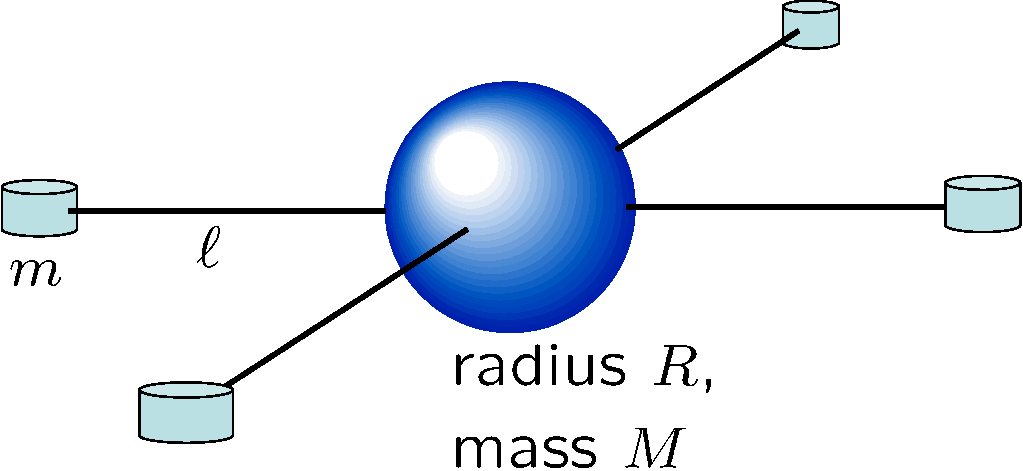
\includegraphics[width=0.6\textwidth]{chap3_multirotor/figures/quadrotor_inertia}\\
  \caption{The moments of inertia for the quadrotor are calculated
  assuming a spherical dense center with mass $M$ and radius $R$,
  and point masses of mass $m$ located at a distance of $\ell$ from
  the center.}%
  \label{fig:quadrotor_inertia}
\end{figure}
As shown in Figure~\ref{fig:quadrotor_inertia}, the quadrotor is
essentially symmetric about all three axes, therefore
$J_{xy}=J_{xz}=J_{yz}=0$ which implies that
\[
\mathbf{J} =
    \begin{pmatrix}
    J_{x}   & 0       & 0 \\
    0       & J_{y}   & 0 \\
    0 & 0       & J_{z}
    \end{pmatrix}.
\]
Therefore
\begin{align*}
\mathbf{J}^{-1}
    &= \begin{pmatrix}
        \frac{1}{J_x} & 0 & 0 \\
        0 & \frac{1}{J_y} & 0 \\
        0 & 0 & \frac{1}{J_z}
       \end{pmatrix}.
\end{align*}
The inertia for a solid sphere is given by
$J=2MR^2/5$\cite{HallidayResnick}.  Therefore
\begin{align*}
J_x &= \frac{2MR^2}{5} + 2\ell^2m \\
J_y &= \frac{2MR^2}{5} + 2\ell^2m \\
J_z &= \frac{2MR^2}{5} + 4\ell^2m.
\end{align*}


Defining $\mathbf{m}^b \defeq (\tau_{\phi}, \tau_{\theta},
\tau_{\psi})^T$ we can write Eq.~\eqref{eq:newton_rotation} in body
coordinates as
\begin{align*}
\begin{pmatrix} \dot{p} \\ \dot{q} \\ \dot{r} \end{pmatrix}
&= \begin{pmatrix}
        \frac{1}{J_x} & 0 & 0 \\
        0 & \frac{1}{J_y} & 0 \\
        0 & 0 & \frac{1}{J_z}
    \end{pmatrix}
    \left[
    \begin{pmatrix}
        0 & r & -q \\
        -r & 0 & p \\
        q & -p & 0
    \end{pmatrix}
    \begin{pmatrix}
    J_{x}   & 0       & 0 \\
    0       & J_{y}   & 0 \\
    0       & 0       & J_{z}
    \end{pmatrix}
    \begin{pmatrix} p \\ q \\ r \end{pmatrix}
    + \begin{pmatrix} \tau_{\phi} \\ \tau_{\theta} \\ \tau_{\psi} \end{pmatrix}
    \right] \\
&= \begin{pmatrix}
    \frac{J_y-J_z}{J_x} qr\\
    \frac{J_z-J_x}{J_y} pr\\
    \frac{J_x-J_y}{J_z} pq\\
    \end{pmatrix}
    + \begin{pmatrix}
    \frac{1}{J_x} \tau_{\phi} \\
    \frac{1}{J_y} \tau_{\theta} \\
    \frac{1}{J_z} \tau_{\psi}
    \end{pmatrix}.
\end{align*}


The six degree of freedom model for the quadrotor kinematics and
dynamics can be summarized as follows:
\begin{align}
\begin{pmatrix} \dot{p}_n \\ \dot{p}_e \\ \dot{h} \end{pmatrix}
&= \begin{pmatrix} c\theta c\psi & s\phi s\theta c\psi - c\phi s\psi
    & c\phi s\theta c\psi + s\phi s\psi \\
    c\theta s\psi &  s\phi s\theta s\psi + c\phi c\psi
    & c\phi s\theta s\psi - s\phi c\psi  \\
    s\theta & -s\phi c\theta & -c\phi c\theta
    \end{pmatrix}
    \begin{pmatrix} u \\ v \\ w \end{pmatrix}
    \label{eq:kin-eom-xyh} \\
\begin{pmatrix} \dot{u} \\ \dot{v} \\ \dot{w} \end{pmatrix}
&= \begin{pmatrix} rv-qw \\ pw-ru \\ qu-pv \end{pmatrix} +
    \frac{1}{m} \begin{pmatrix} f_x \\ f_y \\ f_z \end{pmatrix},
    \label{eq:kin-eom-v}\\
\begin{pmatrix} \dot{\phi} \\ \dot{\theta} \\ \dot{\psi} \end{pmatrix}
& = \begin{pmatrix}
    1 & \sin\phi\tan\theta & \cos\phi\tan\theta \\
    0 & \cos\phi & -\sin\phi \\
    0 & \frac{\sin\phi}{\cos\theta} & \frac{\cos\phi}{\cos\theta}
    \end{pmatrix}
    \begin{pmatrix} p \\ q \\ r \end{pmatrix}
    \label{eq:kin-eom-euler}\\
\begin{pmatrix} \dot{p} \\ \dot{q} \\ \dot{r} \end{pmatrix}
&= \begin{pmatrix}
    \frac{J_y-J_z}{J_x} qr\\
    \frac{J_z-J_x}{J_y} pr\\
    \frac{J_x-J_y}{J_z} pq\\
    \end{pmatrix}
    + \begin{pmatrix}
    \frac{1}{J_x} \tau_{\phi} \\
    \frac{1}{J_y} \tau_{\theta} \\
    \frac{1}{J_z} \tau_{\psi}
    \end{pmatrix}.
    \label{eq:kin-eom-omega}
\end{align}

%%%%%%%%%%%%%%%%%%%%%%%%%%%%%%%%%%%%%%%%%%%%%%%%%%%%%%%%%%%%%
\section{Forces and Moments} \label{chap:forces}
%%%%%%%%%%%%%%%%%%%%%%%%%%%%%%%%%%%%%%%%%%%%%%%%%%%%%%%%%%%%%

The objective of this section is to describe the forces and torques
that act on the quadrotor.  Since there are no aerodynamic lifting
surfaces, we will assume that the aerodynamic forces and moments are
negligible.

The forces and moments are primarily due to gravity and the four
propellers.

\begin{figure}[hhhhtb]
  % Requires \usepackage{graphicx}
  \centering
  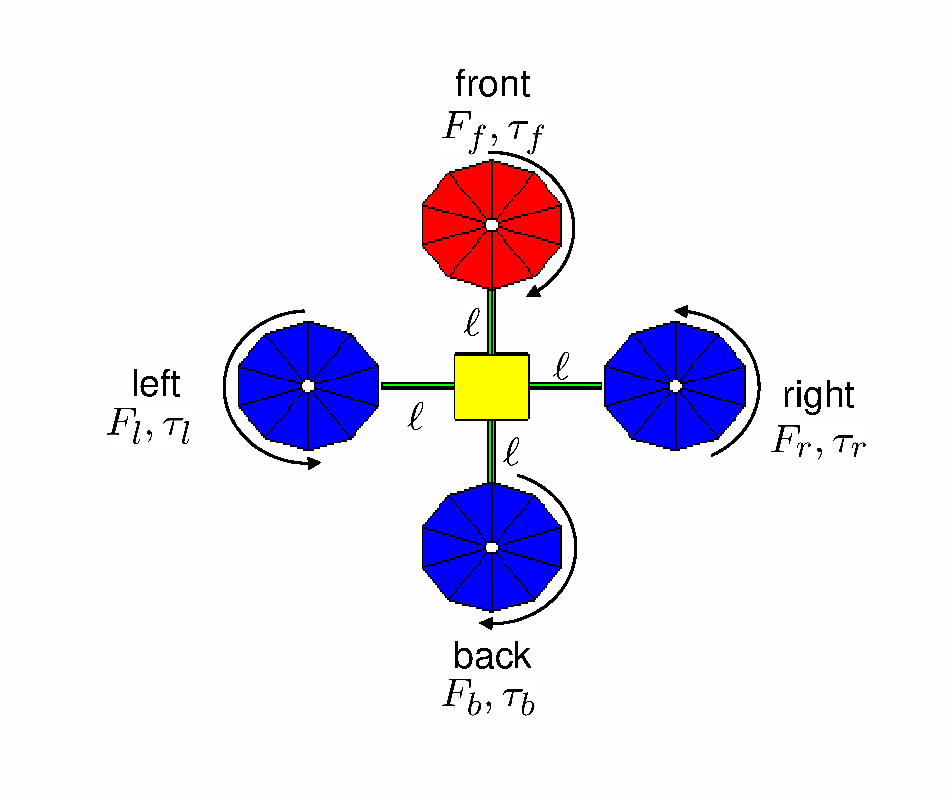
\includegraphics[width=0.6\textwidth]{chap3_multirotor/figures/quadrotor_top_view}\\
  \caption{The top view of the quadrotor.  Each motor produces an upward
  force $F$ and a torque $\tau$.  The front and back motors spin clockwise
  and the right and left motors spin counterclockwise.}%
  \label{fig:quadrotor_top_view}
\end{figure}


\begin{figure}[hhhhtb]
  % Requires \usepackage{graphicx}
  \centering
  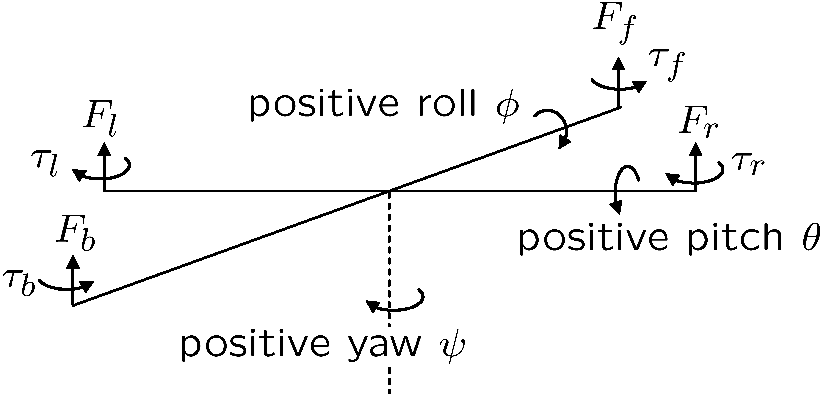
\includegraphics[width=0.6\textwidth]{chap3_multirotor/figures/quadrotor_define_angles}\\
  \caption{Definition of the forces and torques acting on the quadrotor.}%
  \label{fig:quadrotor_define_angles}
\end{figure}


Figure~\ref{fig:quadrotor_top_view} shows a top view of the
quadrotor systems.  As shown in
Figure~\ref{fig:quadrotor_define_angles}, each motor produces a
force $F$ and a torque $\tau$.  The total force acting on the
quadrotor is given by
\[
F = F_f + F_r + F_b + F_l.
\]
The rolling torque is produced by the forces of the right and left
motors as
\[
\tau_{\phi} = \ell(F_l - F_r).
\]
Similarly, the pitching torque is produced by the forces of the
front and back motors as
\[
\tau_{\theta} = \ell(F_f - F_b).
\]
Due to Newton's third law, the drag of the propellers produces a
yawing torque on the body of the quadrotor.  The direction of the
torque will be in the oppositive direction of the motion of the
propeller.  Therefore the total yawing torque is given by
\[
\tau_{\psi} = \tau_r + \tau_l - \tau_f - \tau_b.
\]

The lift and drag produced by the propellers is proportional to the
square of the angular velocity.  We will assume that the angular
velocity is directly proportional to the pulse width modulation
commend sent to the motor.  Therefore, the force and torque of each
motor can be expressed as
\begin{align*}
F_{\ast} &= k_1 \delta_{\ast} \\
\tau_{\ast} &= k_2 \delta_{\ast},
\end{align*}
where $k_1$ and $k_2$ are constants  that need to be determined
experimentally, $\delta_{\ast}$ is the motor command signal, and
$\ast$ represents $f$, $r$, $b$, and $l$.

Therefore, the forces and torques on the quadrotor can be written in
matrix form as
\[
\begin{pmatrix}
    F \\
    \tau_{\phi} \\
    \tau_{\theta} \\
    \tau_{\psi}
\end{pmatrix} =
\begin{pmatrix}
    k_1 & k_1 & k_1 & k_1 \\
    0 & -\ell k_1 & 0 & \ell k_1 \\
    \ell k_1 & 0 & -\ell k_1 & 0 \\
    -k_2 & k_2 & -k_2 & k_2
\end{pmatrix}
\begin{pmatrix}
    \delta_f \\
    \delta_r \\
    \delta_b \\
    \delta_l
\end{pmatrix}
\defeq \mathcal{M}
\begin{pmatrix}
    \delta_f \\
    \delta_r \\
    \delta_b \\
    \delta_l
\end{pmatrix}.
\]

The control strategies derived in subsequent sections will specify
forces and torques.  The actual motors commands can be found as
\[
\begin{pmatrix}
    \delta_f \\
    \delta_r \\
    \delta_b \\
    \delta_l
\end{pmatrix}
= \mathcal{M}^{-1}\emph{}
\begin{pmatrix}
    F \\
    \tau_{\phi} \\
    \tau_{\theta} \\
    \tau_{\psi}
\end{pmatrix}.
\]
Note that the pulse width modulation commands are required to be
between zero and one.


In addition to the force exerted by the motor, gravity also exerts a
force on the quadrotor.  In the vehicle frame $\mathcal{F}^v$, the
gravity force acting on the center of mass is given by
\[
\mathbf{f}_g^v = \begin{pmatrix} 0 \\ 0 \\ mg \end{pmatrix}.
\]
However, since $\mathbf{v}$ in Equation~\eqref{eq:kin-eom-v} is expressed
in $\mathcal{F}^b$, we must transform to the body frame to give
\begin{align*}
\mathbf{f}_g^b &= R_{v}^{b} \begin{pmatrix} 0 \\ 0 \\ mg \end{pmatrix} \\
&= \begin{pmatrix}
  -mg\sin\theta \\ mg\cos\theta\sin\phi \\ mg\cos\theta\cos\phi
  \end{pmatrix}.
\end{align*}

Therefore,
equations~\eqref{eq:kin-eom-xyh}--\eqref{eq:kin-eom-omega} become
\begin{align}
\begin{pmatrix} \dot{p}_n \\ \dot{p}_e \\ \dot{h} \end{pmatrix}
&= \begin{pmatrix} c\theta c\psi & s\phi s\theta c\psi - c\phi s\psi
    & c\phi s\theta c\psi + s\phi s\psi \\
    c\theta s\psi &  s\phi s\theta s\psi + c\phi c\psi
    & c\phi s\theta s\psi - s\phi c\psi  \\
    s\theta & -s\phi c\theta & -c\phi c\theta
    \end{pmatrix}
    \begin{pmatrix} u \\ v \\ w \end{pmatrix}
    \label{eq:kin-eom-xyh2} \\
\begin{pmatrix} \dot{u} \\ \dot{v} \\ \dot{w} \end{pmatrix}
&= \begin{pmatrix} rv-qw \\ pw-ru \\ qu-pv \end{pmatrix}
    + \begin{pmatrix}
  -g\sin\theta \\ g\cos\theta\sin\phi \\ g\cos\theta\cos\phi
  \end{pmatrix}+
    \frac{1}{m} \begin{pmatrix} 0 \\ 0 \\ -F \end{pmatrix},
    \label{eq:kin-eom-v2}\\
\begin{pmatrix} \dot{\phi} \\ \dot{\theta} \\ \dot{\psi} \end{pmatrix}
& = \begin{pmatrix}
    1 & \sin\phi\tan\theta & \cos\phi\tan\theta \\
    0 & \cos\phi & -\sin\phi \\
    0 & \frac{\sin\phi}{\cos\theta} & \frac{\cos\phi}{\cos\theta}
    \end{pmatrix}
    \begin{pmatrix} p \\ q \\ r \end{pmatrix},
    \label{eq:kin-eom-euler2}\\
\begin{pmatrix} \dot{p} \\ \dot{q} \\ \dot{r} \end{pmatrix}
&= \begin{pmatrix}
    \frac{J_y-J_z}{J_x} qr\\
    \frac{J_z-J_x}{J_y} pr\\
    \frac{J_x-J_y}{J_z} pq\\
    \end{pmatrix}
    + \begin{pmatrix}
    \frac{1}{J_x} \tau_{\phi} \\
    \frac{1}{J_y} \tau_{\theta} \\
    \frac{1}{J_z} \tau_{\psi}
    \end{pmatrix}.
    \label{eq:kin-eom-omega2}
\end{align}

%%%%%%%%%%%%%%%%%%%%%%%%%%%%%%%%%%%%%%%%%%%%%%%%%%%%%%%%%%%%%%%5
\section{Simplified Models}

Equations~\eqref{eq:kin-eom-xyh2}--\eqref{eq:kin-eom-omega2} are the
equations of motion to be used in our six degree-of-freedom
simulator.  However, they are not appropriate for control design for
several reasons. The first reason is that they are too complicated
to gain significant insight into the motion.  The second reason is
that the position and orientation are relative to the inertial world
fixed frame, whereas camera measurements will measure position and
orientation of the target with respect to the camera frame.

%----------------------------------------------------------------
\subsection{Model for estimation}
%----------------------------------------------------------------
For the quadrotor, we are not able to estimate the inertial position
or the heading angle $\psi$.  Rather, we will be interested in the
relative position and heading of the quadrotor with respect to a
ground target.  The relative position of the quadrotor will be
measured in the vehicle-1 frame, i.e., the vehicle frame after it
has been rotated by the heading vector $\psi$.  The vehicle-1 frame
is convenient since $x$, $y$, and $z$ positions are still measured
relative to a flat earth, but they are vehicle centered quantities
as opposed to inertial quantities.  Let $p_x$, $p_y$, and $p_z$
denote the relative position vector between the target and the
vehicle resolved in the $v1$ frame.  Therefore
Eq~\eqref{eq:kin-eom-xyh2} becomes
\begin{equation}     \label{eq:kin-eom-xyh3}
\begin{pmatrix} \dot{p}_x \\ \dot{p}_y \\ \dot{p}_z \end{pmatrix}
= \begin{pmatrix} c\theta & s\phi s\theta
    & c\phi s\theta \\
    0 &  c\phi
    & - s\phi  \\
    -s\theta & s\phi c\theta & c\phi c\theta
    \end{pmatrix}
    \begin{pmatrix} u \\ v \\ w \end{pmatrix}.
\end{equation}

%----------------------------------------------------------------
\subsection{Model for control design}
%----------------------------------------------------------------

Assuming that $\phi$ and $\theta$ are small,
Equation~\eqref{eq:kin-eom-euler2} can be simplified as
\begin{equation}\label{eq:kin-eom-euler3}
\begin{pmatrix} \dot{\phi} \\ \dot{\theta} \\ \dot{\psi} \end{pmatrix}
=  \begin{pmatrix} p \\ q \\ r \end{pmatrix}.
\end{equation}
Similarly, Equation~\eqref{eq:kin-eom-omega2} is simplified by
assuming that the Coriolis terms $qr$, $pr$, and $pq$, are small to
obtain
\begin{equation}\label{eq:kin-eom-omega3}
\begin{pmatrix} \dot{p} \\ \dot{q} \\ \dot{r} \end{pmatrix}
=   \begin{pmatrix}
    \frac{1}{J_x} \tau_{\phi} \\
    \frac{1}{J_y} \tau_{\theta} \\
    \frac{1}{J_z} \tau_{\psi}
    \end{pmatrix}.
\end{equation}
Combining Eq.~\eqref{eq:kin-eom-euler3}
and~\eqref{eq:kin-eom-omega3} we get
\begin{equation}\label{eq:kin-euler-ddot}
\begin{pmatrix} \ddot{\phi} \\ \ddot{\theta} \\ \ddot{\psi} \end{pmatrix}
=  \begin{pmatrix}
    \frac{1}{J_x} \tau_{\phi} \\
    \frac{1}{J_y} \tau_{\theta} \\
    \frac{1}{J_z} \tau_{\psi}
    \end{pmatrix}.
\end{equation}

Differentiating Eq.~\eqref{eq:kin-eom-xyh2} and neglecting
$\dot{R}_b^v$ gives
\begin{equation}\label{eq:kin-eom-xyh4}
\begin{pmatrix} \ddot{p}_n \\ \ddot{p}_e \\ \ddot{p}_d \end{pmatrix}
= \begin{pmatrix} c\theta c\psi & s\phi s\theta c\psi - c\phi s\psi
    & c\phi s\theta c\psi + s\phi s\psi \\
    c\theta s\psi &  s\phi s\theta s\psi + c\phi c\psi
    & c\phi s\theta s\psi - s\phi c\psi  \\
    -s\theta & s\phi c\theta & c\phi c\theta
    \end{pmatrix}
    \begin{pmatrix} \dot{u} \\ \dot{v} \\ \dot{w} \end{pmatrix}.
\end{equation}
Neglecting the Coriolis terms and plugging Eq.~\eqref{eq:kin-eom-v2}
into Eq.~\eqref{eq:kin-eom-xyh4} and simplifying gives
\begin{equation}\label{eq:kin-xyh-ddot}
\begin{pmatrix} \ddot{p}_n \\ \ddot{p}_e \\ \ddot{p}_d \end{pmatrix}
= \begin{pmatrix} 0 \\ 0 \\ g \end{pmatrix} +
\begin{pmatrix}
    -c\phi s\theta c\psi - s\phi s\psi \\
    -c\phi s\theta s\psi + s\phi c\psi  \\
    -c\phi c\theta
    \end{pmatrix}
    \frac{F}{m}.
\end{equation}

Therefore, the simplified inertial model is given by
\begin{align}
\ddot{p}_n    &= \left(-\cos\phi \sin\theta \cos\psi - \sin\phi
\sin\psi \right) \frac{F}{m}
\label{eq:quadrotor-simple-pn} \\
\ddot{p}_e    &= \left( -\cos\phi \sin\theta \sin\psi + \sin\phi
\cos\psi \right) \frac{F}{m}
\label{eq:quadrotor-simple-pe} \\
\ddot{p}_d      &= g - \left( \cos\phi \cos\theta \right)
\frac{F}{m}
\label{eq:quadrotor-simple-h} \\
\ddot{\phi}   &= \frac{1}{J_x} \tau_{\phi}
\label{eq:quadrotor-simple-phi} \\
\ddot{\theta} &= \frac{1}{J_y} \tau_{\theta}
\label{eq:quadrotor-simple-theta} \\
\ddot{\psi}   &= \frac{1}{J_z} \tau_{\psi}.
\label{eq:quadrotor-simple-psi} \\
\end{align}

The dynamics given in
Equations~\eqref{eq:quadrotor-simple-pn}--\eqref{eq:quadrotor-simple-psi}
are expressed in the inertial frame.  This is necessary for the
simulator.  However, we will be controlling position, altitude, and
heading using camera frame measurements of a target position.  In
this setting heading is irrelevant.  Therefore, instead of
expressing the translational dynamics in the inertial frame, we will
express them in the vehicle-1 frame $\mathcal{F}^{v1}$, which is
equivalent to the inertial frame after rotating by the heading
angle.

Differentiating Eq.~\eqref{eq:kin-eom-xyh3} and neglecting
$\dot{R}_b^{v1}$ gives
\begin{equation}\label{eq:kin-eom-xyh5}
\begin{pmatrix} \ddot{p}_x \\ \ddot{p}_y \\ \ddot{p}_z \end{pmatrix}
= \begin{pmatrix} c\theta & s\phi s\theta
    & c\phi s\theta \\
    0 &  c\phi
    & - s\phi  \\
    -s\theta & s\phi c\theta & c\phi c\theta
    \end{pmatrix}
    \begin{pmatrix} \dot{u} \\ \dot{v} \\ \dot{w} \end{pmatrix}.
\end{equation}
Neglecting the Coriolis terms and plugging Eq.~\eqref{eq:kin-eom-v2}
into Eq.~\eqref{eq:kin-eom-xyh5} and simplifying gives
\begin{equation}\label{eq:kin-xyh-ddot}
\begin{pmatrix} \ddot{p}_x \\ \ddot{p}_y \\ \ddot{p}_z \end{pmatrix}
= \begin{pmatrix} 0 \\ 0 \\ g \end{pmatrix} +
\begin{pmatrix}
    -c\phi s\theta \\
    s\phi \\
    -c\phi c\theta
    \end{pmatrix}
    \frac{F}{m}.
\end{equation}

Therefore, the simplified model in the vehicle-1 frame is given by
\begin{align}
\ddot{p}_x    &= -\cos\phi \sin\theta \frac{F}{m}
\label{eq:quadrotor-simple-px} \\
\ddot{p}_y    &= \sin\phi \frac{F}{m}
\label{eq:quadrotor-simple-py} \\
\ddot{p}_z    &= g - \cos\phi \cos\theta \frac{F}{m}
\label{eq:quadrotor-simple-pz} \\
\ddot{\phi}   &= \frac{1}{J_x} \tau_{\phi}
\label{eq:quadrotor-simple-phi2} \\
\ddot{\theta} &= \frac{1}{J_y} \tau_{\theta}
\label{eq:quadrotor-simple-theta2} \\
\ddot{\psi}   &= \frac{1}{J_z} \tau_{\psi}.
\label{eq:quadrotor-simple-psi2} \\
\end{align}

} 
%%%%%%%%%%%%%%%%%% End BIG omit

\section{Multirotor Aerial Vehicles, Mahony, Kumar, Corke, IEEE RA Mag, Sept, 2020.}
The model in this paper is nicely done.

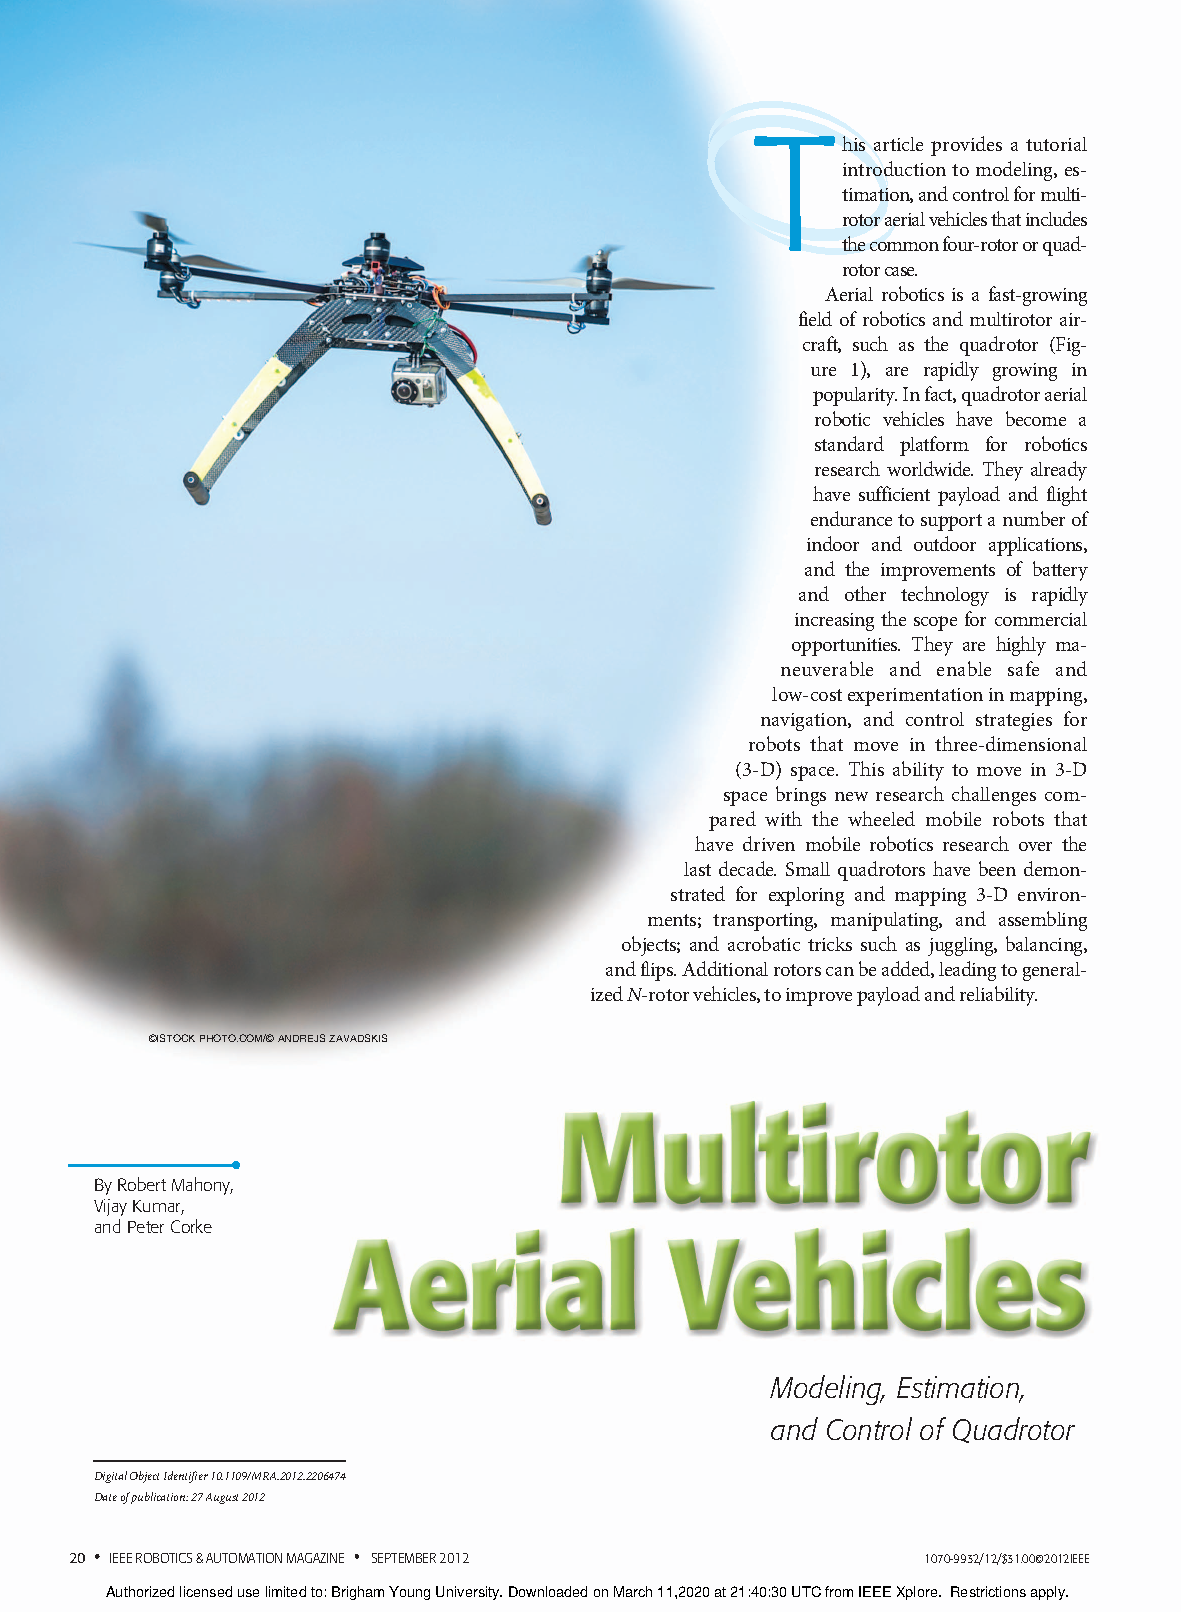
\includepdf[pages=-,scale=.8,pagecommand={}]{chap3_multirotor/papers/MahonyKumarCorke.pdf}





%!TEX root =../quadrotorbook.tex
\chapter{Trajectory Following}
\label{chap:trajectory_following}

In this chapter we discuss trajectory following algorithms for aircraft.  In particular, given an inertially defined trajectory 
\[
\Taubf(t) = \{\pbf_{d/i}^i(t), R_d^i(t)\}
\]
where $\mathcal{F}_d$ is the ``desired'' frame, and where $\pbf_{d/i}^i(t)\in\mathbb{R}^3$ is the desired trajectory of the center of the frame, and $R_d^i(t)\in SO(3)$ is the desired attitude.  The goal is to select the throttle $T$, and the torque $\taubf^b$ so that the multirotor follows the desired trajectory, i.e., 
\begin{align*}
\norm{\pbf_{b/i}^i(t) - \pbf_{d/i}^i} &\to 0, \\
R_d^{i\top} R_b^i \to I.
\end{align*}

For completeness we will discuss several options for trajectory stabilization.  


%%%%%%%%%%%%%%%%%%%%%%%%%%%%%%%%%%%%%%%%%%%%%%%%%%%%%%%%%%%%%%%
\section{A Primer on Lyapunov Stability Theory}

This section provides review of concepts from Lyapunov theory that will be needed to understand the developments in this book, and this chapter in particular.  An excellent resource for this material is (Khalil, 1992)~\cite{Khalil92}.  Given the controlled nonlinear systems 
\[
\dot{x}=\bar{f}(x,u),
\]
suppose that the control strategy is given by $u=k(x)$, then the system can be written as
\[
\dot{x} = \bar{f}(x,k(x)) = f(x).
\]
We say that $x_e$ is an equilibrium of the system if $f(x_e)=0$.

Let $\mathcal{X}$ be the state space, and let $\Omega\subset\mathcal{X}$.  If $x_e\in\Omega$, a function $V:\Omega\to\mathbb{R}$ is said to be {\em positive definite} on $\Omega$ if $V(x)>0$ for all $x\in\Omega\setminus\{x_e\}$ and $V(x_e)=0$.  The function $V$ is said to be {\em positive semi-definite} on $\Omega$ if $V(x)\geq 0$ for all $x\in\Omega$.  Define the level set
\[
\Omega_c = \left\{ x\in\mathcal{X} ~|~ V(x) \leq 0 \right\}.
\]

\begin{theorem}[Lyapunov Theorem] \label{thm:lyapunov_theorem}
If $c>0$ is selected so that $\Omega_c$ is closed and bounded, and if $\dot{V}(t)$ is negative definite on $\Omega_c$, then $\norm{x(t)}\to 0$ as $t\to\infty$.
\end{theorem}

As a simple example, let $x\in\mathbb{R}$, and let $\dot{x}=\sin(u)$, where $u=-kx$.  Note that $\sin(-k\cdot 0)=0$ and so $x_e=0$ is an equilibrium of the system.  Define the Lyapunov function candidate $V(x) = \frac{1}{2}x^2$, which results in 
\[
\dot{V} = x\dot{x} = x\sin(-kx) = -x\sin(kx)
\]
which is less than zero if $x\in (-\pi, \pi)$.  Therefore, pick any $0<c<\pi$, and let $\Omega_c = \{x\in\mathbb{R}  ~|~ \frac{1}{2}x^2 \leq c\}$.  Clearly $\Omega_c$ is closed and bounded, and $\dot{V}<0$ for all $x\in\Omega_c$.  Therefore Theorem~\ref{thm:lyapunov_theorem} guarantees that $\abs{x(t)}\to 0$.

However, there are many relatively straightforward controlled systems for which standard Lyapunov theory is deficient.  For example, consider the second order double integrator system 
$\ddot{y}=u$,
where the control input is the standard feedforward plus proportional-derivative control
\[
u = \ddot{y}_d + k_p(y_d-y) + k_d(\dot{y}_d-\dot{y}).
\]
It is well known that this control law ensures that $y(t)\to y_d(t)$.  Suppose that we would like to demonstrate this fact using Theorem~\ref{thm:lyapunov_theorem}.  Let $\tilde{y} = y-y_d$, and note that
\begin{equation}\label{eq:double_integrator_lasalle}
\dot{\tilde{y}} = \ddot{y}-\ddot{y}_d = u - \ddot{y}_d = -k_p\tilde{y} - k_d\dot{\tilde{y}}.
\end{equation}
Pick the Lyapunov function candidate
\[
V(\tilde{y},\dot{\tilde{y}}) = \frac{k_p}{2}\tilde{y}^2 + \frac{1}{2}\dot{\tilde{y}}^2,
\]
which is positive definite if $k_p>0$.  Differentiating we get
\begin{align*}
\dot{V} &= k_p \tilde{y}\dot{\tilde{y}} + \dot{\tilde{y}}\ddot{\tilde{y}} \\
 	&= \dot{\tilde{y}}\left( k_p	\tilde{y} - k_p\tilde{y} - k_d\dot{\tilde{y}} \right) \\
 	&= - k_d \dot{\tilde{y}}^2.
\end{align*}
If $k_d>0$, then $\dot{V}$ is negative semi-definite since $\tilde{y}$ can be nonzero when $\dot{V}=0$.  Letting 
\[
\Omega_c = \{ (\tilde{y}, \dot{\tilde{y}}) ~|~ V(\tilde{y},\dot{\tilde{y}}) \leq c \}
\]
we note that $\Omega_c$ is closed and bounded for any finite $c$, and that $\dot{V}(x)\leq 0$ on $\Omega_c$.  However, Theorem~\ref{thm:lyapunov_theorem} does not guarantee that $(\tilde{y}(t),\dot{\tilde{y}}(t))\to (0,0)$ because $V$ is not negative definite.  
%
Fortunately, the well known LaSalle Invariance Theorem provides an additional tool that helps in this situation. Before stating the theorem, we need two definitions.
\begin{definition}
The set $\Omega$ is said to be {\em positively invariant} with respect to the dynamics $\dot{x}=f(x)$ if when solutions $x(t)$ enter $\Omega$, they remain in $\Omega$ thereafter.  	
\end{definition}
\begin{definition}
The set $\Omega$ is said to be {\em invariant} with respect to the dynamics $\dot{x}=f(x)$ the solution begin in $\Omega$ at time $s$, i.e., $x(s)\in\Omega$ implies that $x(t)\in\Omega$ for all time $\in (-\infty, \infty)$.  In other words, the only way for $x(t)$ to be in $\Omega$ is if it started there.
\end{definition}
\begin{theorem}[LaSalle Invariance Theorem] \label{thm:lasalle_invariance_theorem}.  
Let $V:\mathcal{X} \mapsto \mathbb{R}$, and select $0<c<\infty$ so that $\Omega_c$ is closed and bounded, and suppose that $\dot{V}(x)\leq 0$ for all $x\in\Omega_c$.
Define $E=\Omega_c\cap \{x\in\Omega_c ~|~ \dot{V}(x) = 0 \}$, and define $M\subset E$ to be the set of all invariant points in $E$.  Then all solutions of the differential equation $\dot{x}=f(x)$ approach $M$ asymptotically as $t\to\infty$.
\end{theorem}

As an example, consider the previous double integrator problem, where we have shown that $\dot{V}=-k_d\dot{\tilde{y}}^2\leq 0$ for all $(\tilde{y},\dot{\tilde{y}})\in\Omega_c$, where $c$ is any finite number.  Therefore
\[
E = \Omega_c \cap \{(\tilde{y}, 0) ~|~ \tilde{y}\in\mathbb{R} \}.
\]
LaSalle's invariance theorem shows that all trajectories $(\tilde{y}(t), \dot{\tilde{y}}(t)) \to M$, where $M$ is the set of invariant points in $E$.  We will now show that $M=\{(0,0)\}$.  Indeed, if the trajectory $(\tilde{y}(t), \dot{\tilde{y}}(t)) \in M \subset E$, then we know that $\dot{\tilde{y}}(s)=0$ for all $s\in (-\infty, \infty)$.  Therefore $\ddot{\tilde{y}}(s)=0$ for all $s\in (-\infty, \infty)$.  From Equation~\eqref{eq:double_integrator_lasalle} we have that $k_d\tilde{y}(s)=0$ for all $s\in (-\infty, \infty)$.  Since $k_d>0$ this implies that $\tilde{y}(s)=0$ for all $s\in (-\infty, \infty)$.  Therefore $M=\{(0,0)\}$ and we have shown that $\norm{y(t)-y_d(t)}\to 0$ as $t\to\infty$.


%%%%%%%%%%%%%%%%%%%%%%%%%%%%%%%%%%%%%%%%%%%%%%%%%%%%%%%%%%%%%%%
\section{Angular Rate Regulation}
We begin by discussing angular rate stabilization.
Recall from Equations~\eqref{eq:eom_omega} that the angular dynamics of the multirotor are given by
\begin{equation}
	J\dot{\omegabf}_{b/i}^b = -\omegabf_{b/i}^b \times (J\omegabf_{b/i}^b) + \taubf^b. 
\end{equation}

Given a desired angular velocity $\omegabf_{d/i}^b$ expressed in the body frame, the objective is to select the torque $\taubf^b$ so that 
\[
\omegabf_{b/i}^b \to  \omegabf_{d/i}^b.
\]
\begin{theorem}\label{thm:angular_rate_regulation}
If the desired angular velocity is given as 	$\omegabf_{d/i}^b(t)$ and is differentiable, and the torque is given by
\begin{equation}\label{eq:torque_angular_velocity}
\taubf^b = \omegabf_{b/i}^b \times (J\omegabf_{b/i}^b) + J\dot{\omegabf}_{d/i}^b - JK\left(\omegabf_{b/i}^b-\omegabf_{d/i}^b\right),
\end{equation}
where $K=K>0$, then $\norm{\omegabf_{b/i}^b(t) -  \omegabf_{d/i}^b(t)} \to 0$.
\end{theorem}
\begin{proof}
Define
\[
\tilde{\omegabf}\defeq \omegabf_{b/i}^b -  \omegabf_{d/i}^b, 
\]
and define the Lyapunov function candidate as
\[
V = \frac{1}{2} \tilde{\omegabf}^\top J \tilde{\omegabf}.
\]
Differentiating we obtain
\begin{align*}
\dot{V} &= \tilde{\omegabf}^\top J \dot{\tilde{\omegabf}} \\
	&= \tilde{\omegabf}^\top \left( J\omegabf_{b/i}^b - J\omegabf_{d/i}^b \right) \\
	&= \tilde{\omegabf}^\top \left( -\omegabf_{b/i}^b \times (J\omegabf_{b/i}^b) + \taubf^b - J\dot{\omegabf}_{d/i}^b \right).
\end{align*}
Selecting the torque as in Equation~\eqref{eq:torque_angular_velocity}, gives
\[
\dot{V} = -\tilde{\omegabf}^\top K \tilde{\omegabf},
\]
implying from Theorem~\ref{thm:lyapunov_theorem}, that $\norm{\tilde{\omegabf}}\to 0$.
\end{proof}

Note that the desired angular velocity in Theorem~\ref{thm:angular_rate_regulation} is given in the body frame.  
Also note that control strategy~\eqref{eq:torque_angular_velocity} requires knowledge of the inertia matrix $J$.  


%%%%%%%%%%%%%%%%%%%%%%%%%%%%%%%%%%%%%%%%%%%%%%%%%%%%%%%%%%%%%%%
\section{Attitude Stabilization Using Euler Angles}

In near hover conditions, the attitude is adequately represented using the Euler angles, and the dynamics are given by
\begin{align*}
	\dot{\Theta} &= S(\Theta)\omegabf_{b/i}^b \\	
	J\dot{\omegabf}_{b/i}^b &= -\omegabf_{b/i}^b \times (J\omegabf_{b/i}^b) + \taubf^b,
\end{align*}
where
\[
S(\Theta)= \begin{pmatrix} 1, & \sin\phi\tan\theta, & \cos\phi\tan\theta \\
 0, & \cos\phi, & -\sin\phi \\
 0, & \sin\phi\sec\theta, & \cos\phi\sec\theta
 \end{pmatrix}
\]
is well defined and invertible for small $\Theta$.  When the roll angle $\phi$ and the pitch angle $\theta$ are small, we have that $S(\Theta)\approx I$, implying that $\dot{\Theta}\approx \omegabf_{b/i}^b$.  Assuming also that $\omega_{b/i}^b$ is small enough that $-\omegabf_{b/i}^b \times (J\omegabf_{b/i}^b)$ can be neglected gives
\[
J\ddot{\Theta} = \taubf^b.
\]
\rwbcomment{Need to add the the derivation of the top equation to the previous chapter.}
Given the desired attitude as $\dot{\Theta}_d(t)$, the objective is design $\taubf^b$ so that $\Theta(t)\to \Theta_d(t)$.

\begin{theorem}\label{thm:euler_attitude_stabilization}
	Given the desired Euler angles $\Theta^d(t)$, and assuming that $\dot{\Theta}^d$ and $\ddot{\Theta}^d$ are well defined, the control law
	\begin{equation}\label{eq:torque_euler_attitude_regulation}
	\taubf^b = J\ddot{\Theta}^d - K_p (\Theta-\Theta^d) - K_v (\dot{\Theta}-\dot{\Theta}^d),
	\end{equation}
	where $K_p=K_p^\top >0$ and $K_v=K_v^\top$, then $\Theta(t)\to\Theta^d(t)$ and $\dot{\Theta}(t)\to\dot{\Theta}^d(t)$.
\end{theorem}
\begin{proof}
Define
\[
\tilde{\Theta} \defeq \Theta - \Theta^d,
\]
and define the Lyapunov function
\[
V(\Theta, \dot{\Theta}) = \frac{1}{2}\tilde{\Theta}^\top K_p \tilde{\Theta} + \frac{1}{2}\dot{\tilde{\Theta}}^\top J \dot{\tilde{\Theta}}.
\]
Differentiating $V$ gives
\begin{align*}
\dot{V} &= \dot{\tilde{\Theta}}^\top K_p	 \tilde{\Theta} + \tilde{\Theta}^\top \left( J\ddot{\Theta} - J\ddot{\Theta}^d\right) \\
	&= \dot{\tilde{\Theta}}^\top \left( K_p	 \tilde{\Theta} + \taubf^b - J\ddot{\Theta}^d) \right).
\end{align*}
Using Equation~\eqref{eq:torque_euler_attitude_regulation} gives
\[
\dot{V} = -\dot{\tilde{\Theta}}^\top K_v \dot{\tilde{\Theta}}.
\]
Define the set $\Omega_c = \{ (\tilde{\Theta},\dot{\tilde{\Theta}}) ~|~ V(\Theta,\dot{\Theta}) < c\}$ and note that if the dynamics are satisfied, then all trajectories that start in $\Omega_c$ remain in $\Omega_c$.  Define
\[
E = \Omega_c \cap \{ (\tilde{\Theta}, \dot{\tilde{\Theta}}) ~|~ \dot{V}(\Theta, \dot{\Theta}) = 0 \},
\]
and let $M$ be the largest invariant set in $E$.  Then for all trajectories in $M$ we must have that $\dot{\Theta}\equiv 0$, which is true if and only if $\ddot{\Theta}\equiv 0$.  Therefore $J\ddot{\tilde{\Theta}} = \taubf^b - J\ddot{\Theta}^d \equiv 0$.  From Equation~\eqref{eq:torque_euler_attitude_regulation} we get that $K_p\tilde{\Theta}\equiv 0$, and therefore that $M = \{(\tilde{\Theta}, \dot{\tilde{\Theta}}) ~|~ \tilde{\Theta} = 0, \dot{\tilde{\Theta}}=0 \}.$, and Theorem~\ref{thm:lasalle_invariance_theorem} implies that all trajectories that start in $\Omega_c$ converge to $M$.
\end{proof}

Note that Equation~\eqref{eq:torque_euler_attitude_regulation} is a standard feedforward plus proportional-derivative feedback control law.  

For many multirotor systems, the low-level autopilot is providing rate feedback using a strategy similar to Theorem~\ref{thm:angular_rate_regulation}.  In that case, if we assume that the inner rate stabilization loop is much faster than the attitude kinematics, then we can assume that $\omegabf_{b/i}^b = \omegabf_c$, where $\omegabf_c$ is the commanded angular velocity, which implies that the equations of motion are simply
\[
\dot{\Theta} = \omegabf_c,
\]
leading to the following simplified strategy for attitude control.
\begin{theorem}\label{thm:euler_attitude_stabilization_simple}
	Given the desired Euler angles $\Theta^d(t)$, and assuming that $\dot{\Theta}^d$ is well defined, the control law
	\begin{equation}\label{eq:euler_attitude_regulation_simple}
	\omegabf_c = \dot{\Theta}^d - K_p (\Theta-\Theta^d),
	\end{equation}
	where $K_p=K_p^\top >0$, then $\Theta(t)\to\Theta^d(t)$.
\end{theorem}
\begin{proof}
Define
\[
\tilde{\Theta} \defeq \Theta - \Theta^d,
\]
and define the Lyapunov function
\[
V = \frac{1}{2}\tilde{\Theta}^\top K_p \tilde{\Theta}.
\]
Differentiating $V$ gives
\begin{align*}
\dot{V} &= \tilde{\Theta}^\top \left(\dot{\Theta} - \dot{\Theta}^d\right) \\
	&= \tilde{\Theta}^\top \left(\omegabf_c - \dot{\Theta}^d\right).
\end{align*}
Using Equation~\eqref{eq:euler_attitude_regulation_simple} gives
\[
\dot{V} = -\tilde{\Theta}^\top K_p \tilde{\Theta}.
\]
From Theorem~\ref{thm:lyapunov} we have that $\norm{\tilde{\Theta}}\to 0$.
\end{proof}

Note that Equation~\eqref{eq:euler_attitude_regulation_simple} is a standard feedforward plus proportional feedback control strategy.

%%%%%%%%%%%%%%%%%%%%%%%%%%%%%%%%%%%%%%%%%%%%%%%%%%%%%%%%%%%%%%%
\section{Attitude Stabilization Using Rotation Matrices}

This section derives a control strategy for attitude stabilization using a purely geometric approach. We assume the attitude dynamics given by
\begin{align}
\dot{R}_b^i &= R_b^i\ss{\omegabf_{b/i}^b} \\
J\dot{\omegabf}_{b/i}^b &= -\omegabf_{b/i}^b \times J\omegabf_{b/i}^b + \boldsymbol{\tau}^b.
\end{align}

Recall from the Rodrigues formula~\eqref{eq:rodrigues_1} that given a unit vector $\mathbf{n}$ and a scalar $\theta$, the associated rotation matrix is
\[
\exp(\theta\mathbf{n}) = R(\theta\mathbf{n}) \doteq I + \sin\theta \ss{\mathbf{n}} + (1-\cos\theta)\ss{\mathbf{n}}^2.
\]
When $\theta = \pi$ we have
\begin{align*}
\exp(\pi\mathbf{n}) &= I + \sin\pi \ss{\mathbf{n}} + (1-\cos\pi)\ss{\mathbf{n}}^2 \\
  &= I + 2(\nbf\nbf^\top - I) \\
  &= 2\nbf\nbf^\top - I.
\end{align*}
Define the set 
\[
U = \{ I\} \cup \left\{2\nbf\nbf^\top - I ~|~ \norm{\nbf}=1  \right\}
\]
to be the set consisting of the identity matrix, and the set of all rotations by an angle of $\pi$.
\begin{lemma}\label{lem:set_U}
If $R\in SO(3)$, then $\mathbb{P}_a(R)=0$ if and only if $R\in U$.
\sidenote{Recall that $\mathbb{P}_a(R) = \frac{1}{2}(R-R^\top)$.}
\end{lemma}
\begin{proof}
Using the Rodrigues formula, for rotation matrix $R$ can be expressed as 
\begin{equation}\label{eq:rodrigues-inner-loop}
R = \exp(\theta \mathbf{n}) = I + \sin\theta \ss{\nbf} + (1-\cos\theta)\ss{\nbf}^2,
\end{equation}
for some $\theta$ and unit vector $\mathbf{n}$.  Therefore 
\begin{align*}
\mathbb{P}_a(R) &= \frac{1}{2}(R-R^\top) \\
                &= \frac{1}{2}\big( I + \sin\theta \ss{\nbf} + (1-\cos\theta) \ss{\nbf}\ss{\nbf} \\
                &\qquad - I - \sin\theta \ss{\nbf}^\top - (1-\cos\theta) (\ss{\nbf}\ss{\nbf})^\top\big) \\
                &= 2 \sin\theta \ss{\nbf} 
\end{align*}
where we have used the fact that $\ss{\nbf}^\top=-\ss{\nbf}$.  If $R\in U$, then $\theta=\pi$ and $\mathbb{P}_a(R)=0$.  Alternatively, if $\mathbb{P}_a(R)=0$ then $\sin\theta=0$ implying that $\theta = m\pi$, where $m=0, \pm 1, \pm 2, \dots$.  Therefore from Equation~\eqref{eq:rodrigues-inner-loop} we have that
\[
R = R(m\pi\mathbf{n}) = I  + 2(\nbf\nbf^\top - I),
\]
which establishes the result.
\end{proof}

We will also need the following result.
\begin{lemma} \label{lem:trace_norm_bound}
If $R\in SO(3)$, then 
\begin{equation}\label{eq:trace_norm_bound}
0 \leq \frac{1}{2}\trace{I-R} \leq 2.
\end{equation}
Furthermore $\frac{1}{2}\trace{I-R}=0$ if and only if $R=I$, and $\frac{1}{2}\trace{I-R}=2$ if and only if $R\in\{2\nbf\nbf-I ~|~ \norm{\nbf}=1\}$.
\end{lemma}
\begin{proof}
Using the Rodrigues formula
\begin{align}
\frac{1}{2}\trace{I-R} &= \frac{1}{2}\trace{I-(I+\sin\theta\ss{\nbf}+(1-\cos\theta)\ss{\nbf}^2)} \notag \\
	&= \frac{1}{2}\trace{-\sin\theta\ss{\nbf}-(1-\cos\theta)(\nbf\nbf^\top-I)} \notag \\
	&= \frac{1}{2}\trace{(1-\cos\theta)(I-\nbf\nbf^\top)} \notag \\
	&= \frac{1}{2}(1-\cos\theta)(\trace{I}-\trace{\nbf\nbf^\top}) \notag \\
	&= \frac{1}{2}(1-\cos\theta)(3-1) \notag \\
	&= 1-\cos\theta. \label{eq:trace_norm_2}
\end{align}
Clearly Equation~\eqref{eq:trace_norm_bound} holds.  If $R=I$, then $\theta=0$ and $\frac{1}{2}\trace{I-R}=0$.  Conversely if $\frac{1}{2}\trace{I-R}=0$ then $\theta = 2\pi m$, where $m$ is even.  In that case, the Rodrigues formula implies that $R=I$.  On the other hand, Equation~\eqref{eq:trace_norm_2} implies that $\frac{1}{2}\trace{I-R}=2$ if and only if $\theta=\pi$, which from Rodrigues formula is true if and only if $R\in\{2\nbf\nbf^\top-I ~|~ \norm{\nbf}=1\}$.
\end{proof}

\begin{theorem}
Suppose that the attitude dynamics are given by
\begin{align}
\dot{R}_b^i &= R_b^i\ss{\omegabf_{b/i}^b} \\
J\dot{\omegabf}_{b/i}^b &= -\omegabf_{b/i}^ \times J\omegabf_{b/i}^b + \taubf^b,
\end{align}
and that the commanded attitude and angular velocity satisfy
\[
\dot{R}_d^i = R_d^i \ss{\omegabf_{d/i}^d}
\]
where $\dot{\omegabf}_{d/i}^d$ is continuous.  
Define 
\begin{align*}
	R_d^b &= R_b^{i\top} R_d^i, \\
	\tilde{\omegabf}&=\omegabf_{b/i}^b-R_d^b\omegabf_{d/i}^d
\end{align*}
 and define
\begin{align*}
V(R_d^b,\tilde{\omegabf}) &\defeq \frac{k_p}{2} \trace{I-R_d^b} + \frac{1}{2} \tilde{\omegabf}^\top  J \tilde{\omegabf} \\
\Omega_{c} &\defeq \left\{(R_d^b,\tilde{\omegabf}) ~|~ V(R_d^b,\omegabf)\leq c\right\},
\end{align*}
where $k_p>0$ and $0<c<2k_p$.
If the initial conditions satisfy $(R_d^b(0),\omegabf(0))\in \Omega_c$ and if the torque is given by
\begin{equation}\label{eq:inner-loop-rotation-torque}
\taubf^b = \omegabf_{b/i}^b \times J \omegabf_{b/i}^b + J\left(-\ss{\omegabf_{b/i}^b}R_d^b\omegabf_{d/i}^d + R_d^b\dot{\omegabf}_{d/i}^d\right) + k_p \mathbb{P}_a(R_d^b)^\vee - K_d\tilde{\omegabf} 
\end{equation}
where $K_d=K_d^\top >0$, then $(R_d^b(t), \tilde{\omegabf}(t)) \to (I, \zerobf)$ asymptotically.
\end{theorem}
\begin{proof}
It is clear that $V(R_d^b,\tilde{\omegabf})$ is positive definite and radially unbounded in $\tilde{\omegabf}$.
Differentiating $V$ we get
\begin{align*}
\dot{V} &= -\frac{k_p}{2} \trace{\dot{R}_b^{i\top} R_d^i + R_b^{i\top} \dot{R}_d^i}+ \tilde{\omegabf}^\top ( -\omegabf_{b/i}^b \times J\omegabf_{b/i}^b + \taubf^b - J\dot{\omegabf}_{d/i}^b) \\
        &= -\frac{k_p}{2} \trace{-\ss{\omegabf_{b/i}^b} R_b^{i\top} R_d^i + R_b^{i\top} R_d^i\ss{\omegabf_{d/i}^d} } + \tilde{\omegabf}^\top ( -\omegabf_{b/i}^b \times J\omegabf_{b/i}^b + \taubf^b - J\dot{\omegabf}_{d/i}^b) \\
        &= -\frac{k_p}{2} \trace{-\ss{\omegabf_{b/i}^b} R_d^b + R_d^b \ss{\omegabf_{d/i}^d}R_d^{b\top} R_d^b } + \tilde{\omegabf}^\top ( -\omegabf_{b/i}^b \times J\omegabf_{b/i}^b + \taubf^b - J\dot{\omegabf}_{d/i}^b) \\
        &= -\frac{k_p}{2} \trace{-\ss{\omegabf_{b/i}^b} R_d^b + \ss{R_d^b \omegabf_{d/i}^d} R_d^b } + \tilde{\omegabf}^\top ( -\omegabf_{b/i}^b \times J\omegabf_{b/i}^b + \taubf^b - J\dot{\omegabf}_{d/i}^b) \\
        &= -\frac{k_p}{2} \trace{-\ss{\tilde{\omegabf}} R_d^b } + \tilde{\omegabf}^\top ( -\omegabf_{b/i}^b \times J\omegabf_{b/i}^b + \taubf^b - J\dot{\omegabf}_{d/i}^b),
\end{align*}
where we note that
\begin{align*}
\dot{\omegabf}_{d/i}^b &= \frac{d}{dt}\left(R_b^{i\top}R_d^i\omegabf_{d/i}^d\right) \\
	&=	\dot{R}_b^{i\top}R_d^i\omegabf_{d/i}^d + R_b^{i\top}\dot{R}_d^i\omegabf_{d/i}^d + R_b^{i\top}R_d^i\dot{\omegabf}_{d/i}^d \\
	&=	-\ss{\omegabf_{b/i}^b} R_b^{i\top} R_d^i\omegabf_{d/i}^d + R_b^{i\top}R_d^i\ss{\omegabf_{d/i}^d}\omegabf_{d/i}^d + R_b^{i\top}R_d^i\dot{\omegabf}_{d/i}^d \\
	&=	-\ss{\omegabf_{b/i}^b} R_b^{i\top} R_d^i\omegabf_{d/i}^d  + R_b^{i\top}R_d^i\dot{\omegabf}_{d/i}^d.
\end{align*}
\marginnote{We have used the fact that $\ss{\omegabf}\omegabf = \omegabf \times \omegabf = 0$.}

Using the fact that $R_d^b=\mathbb{P}_s(R_d^b)+\mathbb{P}_a(R_d^b)$ we get
\begin{align*}
\dot{V} &= -\frac{k_p}{2} \trace{-\ss{\tilde{\omegabf}} (\mathbb{P}_s(R_d^b)+\mathbb{P}_a(R_d^b) } + \tilde{\omegabf}^\top ( -\omegabf_{b/i}^b \times J\omegabf_{b/i}^b + \taubf^b - J\dot{\omegabf}_{d/i}^b) \\
\dot{V} &= -\frac{k_p}{2} \trace{-\ss{\tilde{\omegabf}} \mathbb{P}_a(R_d^b) } + \tilde{\omegabf}^\top ( -\omegabf_{b/i}^b \times J\omegabf_{b/i}^b + \taubf^b - J\dot{\omegabf}_{d/i}^b) \\
\dot{V} &= -\tilde{\omegabf}^\top k_p\mathbb{P}_a(R_d^b)^\vee + \tilde{\omegabf}^\top ( -\omegabf_{b/i}^b \times J\omegabf_{b/i}^b + \taubf^b - J\dot{\omegabf}_{d/i}^b) \\
\dot{V} &= \tilde{\omegabf}^\top ( -\omegabf_{b/i}^b \times J \omegabf_{b/i}^b + \taubf^b - J\dot{\omegabf}_{d/i}^b - k_p\mathbb{P}_a(R_d^b)^\vee ),
\end{align*}
where we have used property~\eqref{eq:trace_property_4} to obtain the second line, and property~\eqref{eq:trace_property_5} to obtain the third line.
Using the torque in Equation~\eqref{eq:inner-loop-rotation-torque} gives
\[
\dot{V} = -\tilde{\omegabf}^\top K \tilde{\omegabf},
\]
which is negative semi-definite.  Define the sets
\begin{align*}	
E &= \Omega_c \cap \{(R_d^b,\tilde{\omegabf})| \tilde{\omegabf}^\top K \tilde{\omegabf}=0\}
\end{align*}
and let $M$ be the largest invariant set in $E$.  Since the system starts in $\Omega_c$, and $\dot{V}\leq 0$ in $\Omega_c$, all system trajectories remain in $\Omega_c$.  
Define $M$ to be the largest invariant set in $E$.  For trajectories in $M$, we must have that $\tilde{\omegabf}\equiv 0$ which implies that $J\dot{\tilde{\omegabf}}\equiv 0$,
which implies that
\begin{align*}
J(\dot{\omegabf}_{b/i}^b-\dot{\omegabf}_{d/i}^b) &= -\omegabf_{b/i}^b \times J\omegabf_{b/i}^b + \taubf - J\dot{\omegabf}_{d/i}^b \\
	&= -k_p\mathbb{P}_a(R_d^b)^\vee - K_d\tilde{\omegabf} \\
	&= -k_p\mathbb{P}_a(R_d^b)^\vee \\
	&\equiv 0.
\end{align*}
Therefore for all trajectories in $M$ we have that $\mathbb{P}_a(R_d^b)\equiv 0$, which implies that $M = \{I\} \times \{0\}$ from Lemmas~\ref{lem:set_U} and~\ref{lem:trace_norm_bound}.
The LaSalle's invariance theorem therefore guarantees that trajectories starting in $\Omega_c$ approach $M$ asymptotically. 
\end{proof}

For many multirotor systems, the low-level autopilot is providing rate feedback using a strategy similar to Theorem~\ref{thm:angular_rate_regulation}.  In that case, if we assume that the inner rate stabilization loop is much faster than the attitude kinematics, then we can assume that $\omegabf_{b/i}^b = \omegabf_c^b$, where $\omegabf_c^b$ is the commanded angular velocity expressed in the body frame, which implies that the rotational equations of motion are simply
\begin{equation}\label{eq:Rdot_commanded}
\dot{R}_b^i = R_b^i \ss{\omegabf_c^b}
\end{equation}
leading to the following simplified strategy for attitude control.
\begin{theorem}\label{thm:attitude_stabilization_rotation_simple}
	Suppose that the attitude dynamics are given by Equation~\eqref{eq:Rdot_commanded}, and that the desired attitude and angular velocity satisfy
	\[
	\dot{R}_d^i = R_d^i \ss{\omegabf_{d/i}^d}.
	\]
	Suppose that the initial conditions satisfy
	\[
	\frac{1}{2}\trace{I-R_b^{i\top}(0)R_d^i(0)} < 2
	\]
	and that the commanded angular velocity satisfies
	\begin{equation}\label{eq:attitude_stabilization_rotation_simple}
		\omegabf_c^b = R_b^{i\top}R_d^i \omegabf_{d/i}^d + K_p \mathbb{P}_a(R_b^{i\top}R_d^i)^\vee
	\end{equation}
	where $K=K^\top >0$, then $R_b^i(t) \to R_d^i(t)$ asymptotically.
\end{theorem}
\begin{proof}
Define the Lyapunov function
\[
V = \frac{1}{2}\trace{I-R_d^b},
\]
where $R_d^b=R_b^{i\top}R_d^i$,
and take the derivative to get
\begin{align*}
\dot{V} &= -\frac{1}{2}\trace{\dot{R}_d^b} \\
	&= 	-\frac{1}{2}\trace{\dot{R}_b^{i\top}R_d^i + R_b^{i\top}\dot{R}_d^i} \\
	&=  -\frac{1}{2}\trace{-\ss{\omegabf_c^b}R_b^{i\top}R_d^i + R_b^{i\top}R_d^i\ss{\omegabf_{d/i}^d}} \\
	&=  -\frac{1}{2}\trace{-\ss{\omegabf_c^b}R_b^{i\top}R_d^i + R_d^b\ss{\omegabf_{d/i}^d}R_d^{b\top}R_d^b} \\
	&=  -\frac{1}{2}\trace{-\ss{\omegabf_c^b}R_b^{i\top}R_d^i + \ss{R_d^b\omegabf_{d/i}^d}R_d^b} \\
	&=  -\frac{1}{2}\trace{\ss{R_d^b\omegabf_{d/i}^d-\omegabf_c^b}(\mathbb{P}_s(R_d^b)+\mathbb{P}_a(R_d^b))} \\
	&=  -\frac{1}{2}\trace{\ss{R_d^b\omegabf_{d/i}^d-\omegabf_c^b}\mathbb{P}_a(R_d^b)} \\
	&=  (R_d^b\omegabf_{d/i}^d-\omegabf_c^b)^\top \mathbb{P}_a(R_d^b)^\vee.
\end{align*}
Using Equation~\eqref{eq:attitude_stabilization_rotation_simple} gives
\[
\dot{V} = -(\mathbb{P}_a(R_d^b)^\vee)^\top K_p \mathbb{P}_a(R_d^b)^\vee,
\]
which implies that $\mathbb{P}_a(R_d^b) \to 0$.  The initial conditions and Lemma~\ref{lem:trace_norm_bound} ensures that 
$R_b^{i\top}R_d^i \to I$.
\end{proof}

Note that if $R_d^i(t)$ is given and $\dot{R}_d^i(t)$ is ether given or computed numerically, then $\omega_{d/i}^d$ can be computed as
\[
\omega_{d/i}^d(t) = \left( R_d^{i\top}(t) \dot{R}_d^i(t) \right)^\vee.
\]


%%%%%%%%%%%%%%%%%%%%%%%%%%%%%%%%%%%%%%%%%%%%%%%%%%%%%%%%%%%%%%%
\section{Attitude Stabilization Using Quaternions}



%%%%%%%%%%%%%%%%%%%%%%%%%%%%%%%%%%%%%%%%%%%%%%%%%%%%%%%%%%%%%%%
\section{Velocity controller}
\label{sec:velocity_controller}
\rwbcomment{Add proof and flesh out section}

\begin{theorem}
	Given the dynamics 
	\[
	\dot{\vbf}_{b/i}^i = g\ebf_3 - T_c R_d^i\ebf_3
	\]
	and the desired velocity $\vbf_{d/i}^i$ and heading direction $\sbf_{\psi_d}$,
	if the throttle and desired rotation matrix are selected as
	\begin{align*}
		T_c &= \left(g\ebf_3 - K_d\left(\vbf_{d/i}^i-\vbf_{b/i}^i\right)\right)^\top R_b^i\ebf_3 \\
		\rbf_{3d} &= \frac{g\ebf_3 - K_d\left(\vbf_{d/i}^i-\vbf_{b/i}^i\right)}{\norm{g\ebf_3 - K_d\left(\vbf_{d/i}^i-\vbf_{b/i}^i\right)}} \\
		\rbf_{2d} &= \frac{\rbf_{3d} \times \sbf_{\psi_d}}{\norm{\rbf_{3d} \times \sbf_{\psi_d}}} \\
		\rbf_{1d} &= \rbf_{2d} \times \rbf_{3d},
	\end{align*}
	where $K_d=K_d^\top > 0$, and where the desired angular velocity is given by
	\[
	\omegabf_{d/i}^d = (R_d^{i\top}\dot{R}_d^{i})^\vee,
	\]
	then $\norm{\vbf_{b/i}^i - \vbf_{d/i}^i} \to 0$ and $\psi \to \psi_d$.
\end{theorem}

\begin{proof}
	\rwbcomment{need to add, but similar to stuff we have done before.}
\end{proof}



%%%%%%%%%%%%%%%%%%%%%%%%%%%%%%%%%%%%%%%%%%%%%%%%%%%%%%%%%%%%%%%
\section{Trajectory Tracking Control}
Suppose that we are given a desired inertial frame trajectory given by
\[
\mathcal{T}(t) = \{ \pbf_d(t), \dot{\pbf}_d(t), \ddot{\pbf}_d(t), \psi_d(t), \dot{\psi}_d(t) \}
\]
the objective is to design a control strategy so that the multirotor follows the trajectory.


%+++++++++++++++++++++++++++++++++++++++++++++++++++++++++++++
\subsection{Cascaded Control}
We will first derive a control law based on the cascaded control architecture shown in Figure~\ref{fig:cascaded_trajectory_following}.
\begin{marginfigure}[1in]
  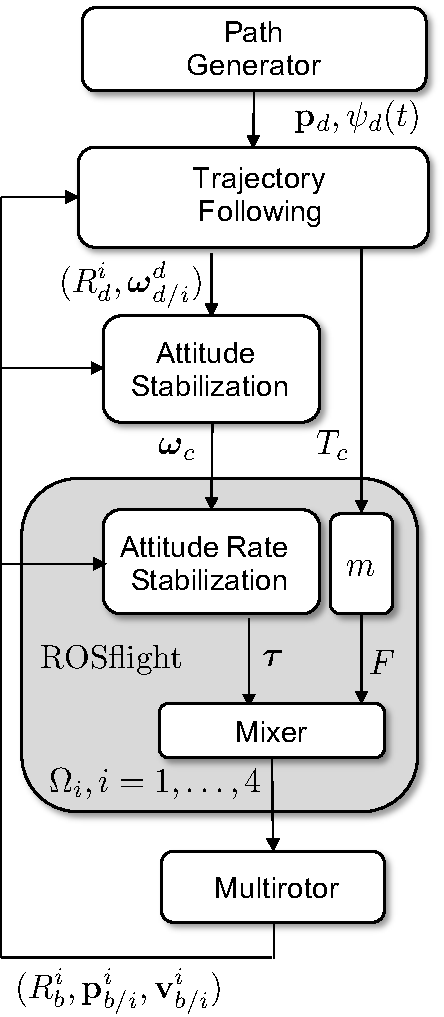
\includegraphics[width=\linewidth]{chap4_trajectory_following/figures/cascaded_trajectory_following}
  \caption{Cascade control architecture for trajectory following.}
  \label{fig:cascaded_trajectory_following}  
\end{marginfigure}
We will assume that the low-level autopilot (labeled ROSflight in Figure~\ref{fig:cascaded_trajectory_following}) implements attitude rate stabilization and accepts a commanded angular velocity $\omegabf_c$, which is the commanded angular velocity of the body relative to the inertial frame, expressed in the body frame, and the commanded throttle $T_c$, which is the commanded force divided by the mass $m$.
The commanded angular rate is supplied by an attitude stabilization loop similar to that derived in Theorem~\ref{thm:attitude_stabilization_rotation_simple}.  
In this section we derive the trajectory following algorithm, where the inputs are the desired inertial position of the multirotor $\pbf_d$, and the desired heading angle $\psi_d$, and their derivatives.

From Equations~\eqref{eq:eom_p}--\eqref{eq:eom_v}, the translational equations of motion are given by
\begin{align}
	\dot{\pbf}_{b/i}^i &= \vbf_{b/i}^i \label{eq:following_pdot_1} \\
	\dot{\vbf}_{b/i}^i &= g \ebf_3 - T_c R_d^i \ebf_3, \label{eq:following_vdot_1}
\end{align}
where we have replaced the throttle $T$ with the commanded throttle $T_c$, and the rotation matrix $R_b^i$ with the desired attitude $R_d^i$, and where we have ignored the induced drag term.
Define the position error as $\tilde{\pbf} \doteq \pbf_{b/i}^i - \pbf_d$, from which we obtain
\begin{equation} \label{eq:cascaded_pddot}
\ddot{\tilde{\pbf}} = g \ebf_3 - T_cR_d^i \ebf_3 - \ddot{\pbf}_d.
\end{equation}

Let the desired rotation matrix be given by
\[
R_d^i = \begin{pmatrix} \rbf_{1d} & \rbf_{2d} & \rbf_{3d} \end{pmatrix},
\]
from which we get
\[
\ddot{\tilde{\pbf}} = g \ebf_3 - T_c\rbf_{3d} - \ddot{\pbf}_d.
\]
The idea behind the trajectory following scheme is to set $T_c\rbf_{3d}$ to achieve PD-like following properties, and then to pick $\rbf_{2d}$ and $\rbf_{1d}$ to align the front of the multirotor with the direction vector
\[
\sbf_{\psi_d} \doteq \begin{pmatrix} \cos\psi_d \\ \sin\psi_d \\  0 \end{pmatrix}.
\]
Toward that end, we have the following scheme.
\begin{theorem}
Given the dynamics in Equation~\eqref{eq:following_pdot_1} and~\eqref{eq:following_vdot_1}, and the desired trajectory given by $\pbf_d(t)$, $\dot{\pbf}_d$, $\ddot{\pbf}_d$, $\psi_d$, $\dot{\psi}_d$, if the throttle and desired rotation matrix are selected as
\begin{align}
T_c &= \norm{\ddot{p}_d - g\ebf_3 - K_p \tilde{\pbf} - K_d\dot{\tilde{\pbf}}} \label{eq:cascaded_attitude_T_c} \\
\rbf_{3d} &= -\frac{\ddot{p}_d - g\ebf_3 - K_p \tilde{\pbf} - K_d\dot{\tilde{\pbf}}}{\norm{\ddot{p}_d - g\ebf_3 - K_p \tilde{\pbf} - K_d\dot{\tilde{\pbf}}}} \label{eq:cascaded_attitude_r_3} \\
\rbf_{2d} &= \frac{\rbf_{3d} \times \sbf_{\psi_d}}{\norm{\rbf_{3d} \times \sbf_{\psi_d}}} \label{eq:cascaded_attitude_r_2}\\
\rbf_{1d} &= \rbf_{2d} \times \rbf_{3d},\label{eq:cascaded_attitude_r_1}
\end{align}
where $K_p=K_p^\top > 0$ and $K_d=K_d^\top > 0$, and where the desired angular velocity is given by
\[
\omegabf_{d/i}^d = (R_d^{i\top}\dot{R}_d^{i})^\vee,
\]
then $\norm{\pbf_{b/i}^i - \pbf_d} \to 0$ and $\psi \to \psi_d$.
\end{theorem}
Note that $R_d^i = (\rbf_{1d}, \rbf_{2d}, \rbf_{3d})$ has been constructed so that the desired body $z$-axis is aligned with the desired acceleration vector, and the body $x$-axis has been aligned so that it is in plane defined by the desired heading direction and the desired acceleration vector.

\begin{proof}
Substituting Equations~\eqref{eq:cascaded_attitude_T_c} and~\eqref{eq:cascaded_attitude_r_3} into Equation~\eqref{eq:cascaded_pddot} gives
\begin{equation} \label{eq:cascaded_pddot}
\ddot{\tilde{\pbf}} = -K_p\tilde{\pbf} - K_d\dot{\tilde{\pbf}}.
\end{equation}
Define the Lyapunov function 
\[
V(\tilde{\pbf},\dot{\tilde{\pbf}}) = \frac{1}{2}\tilde{\pbf}^\top K_p \tilde{\pbf} + \frac{1}{2}\dot{\tilde{\pbf}}^\top \dot{\tilde{\pbf}},
\]
and differentiate to get,
\begin{align*}
\dot{V} &= \dot{\tilde{\pbf}}^\top K_p \tilde{\pbf} + \dot{\tilde{\pbf}}^\top \ddot{\tilde{\pbf}} \\
	&= \dot{\tilde{\pbf}}^\top \left(\ddot{\tilde{\pbf}} + K_p \tilde{\pbf} \right) \\
	&= -\dot{\tilde{\pbf}}^\top K_d \dot{\tilde{\pbf}}.
\end{align*}
Note that if there are no limits on throttle, then $\Omega_c = \{ (\tilde{\pbf}, \dot{\tilde{\pbf}}) ~|~ V \leq c \}$ can be defined by any $c$.  However, if there are throttle limits, then $\Omega_c$ is defined by those limits through Equation~\eqref{eq:cascaded_attitude_T_c}.  
Let 
\[
E=\Omega_c \cap \{(\tilde{\pbf},\dot{\tilde{\pbf}}) ~|~ \dot{V} = 0\} = \Omega_c \cap \{(\tilde{\pbf},\dot{\tilde{\pbf}}) ~|~ \dot{\tilde{\pbf}}\},
\]
and let $M$ be the set of invariant points in $E$.  Then $(\tilde{\pbf},\dot{\tilde{\pbf}})\in M $ implies that $\dot{\tilde{p}}(t)\equiv 0$, where the $\equiv$ symbol is used to mean that the equality holds for all time $t\in (-\infty, \infty)$.  This implies that $\ddot{\tilde{\pbf}}\equiv 0$, which implies from \eqref{eq:cascaded_pddot} that $\tilde{\pbf}\equiv 0$.  Therefore from Theorem~\ref{thm:lasalle_invariance_theorem} $\norm{\tilde{\pbf}}\to 0$.  The attitude stabilization block ensures that $R_b^i(t) \to R_d^i(t)$, and therefore that $\psi(t)\to\psi_d(t)$.
\end{proof}

Additional stuff:

Let 
\[
V=\frac{1}{2}\tilde{\pbf}^\top K_p \tilde{\pbf} + \frac{1}{2}\dot{\tilde{\pbf}}^\top \dot{\tilde{\pbf}}.
\]
Differentiate to get
\begin{align*}
\dot{V} &= \dot{\tilde{\pbf}}^\top \left[ K_p\tilde{\pbf} + g\ebf_3 - TR_b^i\ebf_3 -\ddot{\pbf}_d \right]
\dot{V} &= \dot{\tilde{\pbf}}^\top \left[ K_p\tilde{\pbf} + g\ebf_3 - T\rbf_3 -\ddot{\pbf}_d \right]
\end{align*}
Add and subtract $T\rbf_{3d}/(\rbf_3^\top \rbf_{3d})$ to get
\begin{align*}
\dot{V} &= \dot{\tilde{\pbf}}^\top \left[ K_p\tilde{\pbf} + g\ebf_3 - \frac{T\rbf_{3d}}{(\rbf_3^\top \rbf_{3d})}  -\ddot{\pbf}_d  \left(\frac{(\frac{T\rbf_{3d}}{(\rbf_3^\top \rbf_{3d})})T\rbf_{3}}{(\rbf_3^\top \rbf_{3d})}-\frac{T\rbf_{3d}}{(\rbf_3^\top \rbf_{3d})}\right)\right] \\
&= \dot{\tilde{\pbf}}^\top \left[ K_p\tilde{\pbf} + g\ebf_3 - \frac{T\rbf_{3d}}{(\rbf_3^\top \rbf_{3d})}  -\ddot{\pbf}_d  \left(\frac{T}{(\rbf_3^\top \rbf_{3d})}\right)(I-\rbf_3\rbf_3^\top)\rbf_{3d}\right].
\end{align*}
Now pick
\begin{align*}
\abf_d &= -\ddot{\pbf}_d + g\ebf_3 + K_p\tilde{\pbf} + K_d\dot{\tilde{\pbf}} \\	
\rbf_{3d} &= \frac{\abf_d}{\norm{\abf_d}} \\
T_c &= \abf_d^\top \rbf_3
\end{align*}
resulting in 
\[
\dot{V} = -\dot{\tilde{\pbf}}^\top K_v \dot{\tilde{\pbf}} + \dot{\tilde{\pbf}}^\top (I-\rbf_3\rbf_3^\top )\abf_d.
\]

\rwbcomment{Need to better explain the inner product with $R_b^i \ebf_3$.  Worst case, follow proof of attached paper, but simplify to rotational kinematics.}


%%%%%%%%%%%%%%%%%%%%%%%%%%%%%%%%%%%%%%%%%%%%%%%%%%%%%%%%%%%%%%%
\section{Geometric Tracking Control of a Quadrotor {UAV} on $SE(3)$.}
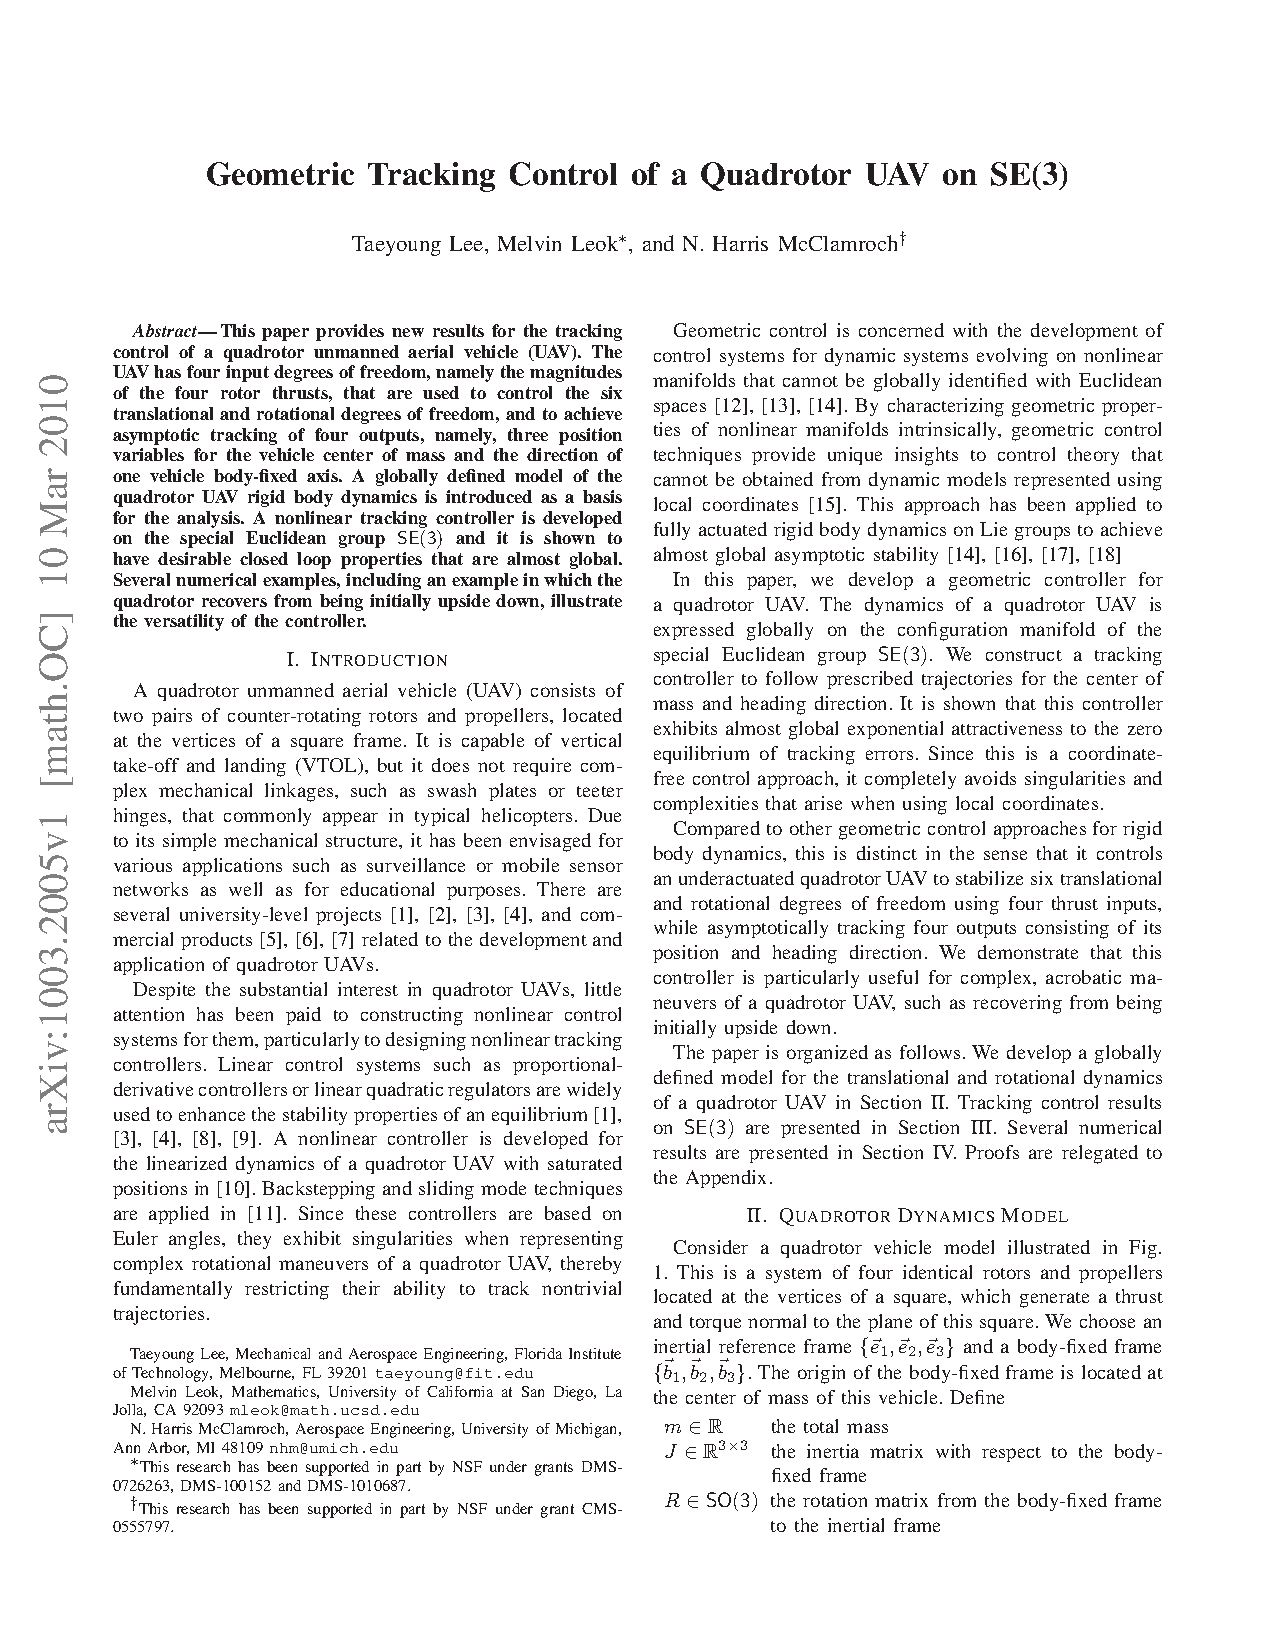
\includepdf[pages=-,scale=.8,pagecommand={}]{chap4_trajectory_following/papers/LeeLeokMcClamroch10_with_proofs.pdf}


%%%%%%%%%%%%%%%%%%%%%%%%%%%%%%%%%%%%%%%%%%%%%%%%%%%%%%%%%%%%%%%
\section{Trajectory following using LQR}

\rwbcomment{develop error state trajectory follower using LQR framework}





%!TEX root =../quadrotorbook.tex
\chapter{Trajectory Generation and Local Planning}
\label{chap:trajectory_planning}

The objective of this chapter is to plan trajectories through a map that represents a cluttered world environment.  The high-level architecture for this chapter is shown in Figure~\ref{fig:planning_architecture}.
\begin{marginfigure}[3in]
  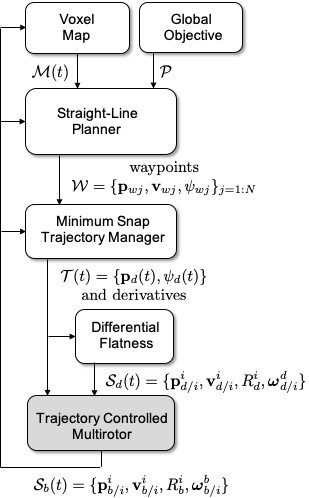
\includegraphics[width=\linewidth]{chap5_trajectory_planning/figures/planning_architecture}
  \caption{The path planning architecture outlined in this chapter.}
  \label{fig:planning_architecture}  
\end{marginfigure}
At the highest level is a voxel representation of the world, local the the multirotor.  The voxel grid will evolve dynamically so that the multirotor always remains in voxel at the center of the map.  A straight-line path planner is then used to plan paths through the voxel map that minimize the distance to the goal location as well as minimize the associated risk.  The output of the straight-line planner is a set of waypoints $\mathcal{W}$ specified as a sequence of desired positions, desired velocities, and desired heading directions.  The waypoints are processed by the {\em minimum-snap trajectory} block to produce a time trajectory of position and heading where the fourth derivative (snap) of the position trajectory is minimized.  The trajectory can be fed directly into the trajectory following framework discussed in Chapter~\ref{chap:trajectory_following}.  However, the framework in Chapter~\ref{chap:trajectory_following} also requires velocity, and angular velocity of the desired multirotor frame.  Those elements are naturally produced by the {\em differential flatness} block shown in Figure~\ref{fig:planning_architecture}.


%----------------------------------
\section{Differential Flatness}
\label{sec:differential_flatness}

Consider the nonlinear system
\begin{equation}\label{eq:flat-system}
\dot{x} = f(x,u),
\end{equation}
where $x$ is the state and $u\in\mathbb{R}^m$ is the control input, and the output mapping
\begin{equation}\label{eq:flat-output}
z = h(x),
\end{equation}
where $z\in\re^p$.  We say that the system~\eqref{eq:flat-system} is differentially flat with flat output $z$ if the following conditions hold~\cite{CowlingYakimenkoWhidborne07}:
\begin{enumerate}
\item The components of $z$ are not differentially related over time.
\item The states $x$ can be written as a function of the flat output and its derivatives, i.e., there exists a function $g_1$, and a finite scalar $m_1$ such that
    \begin{equation}\label{eq:flat-g1}
    x(t) = g_1\left(z(t),\frac{d}{dt}z(t),\cdots,\frac{d^{m_1}}{dt^{m_1}}z(t)\right).
    \end{equation}
\item The control inputs $u$ can be written as a function of the flat output and its derivatives, i.e., there exists a function $g_2$ and a finite scalar $m_2$ such that
    \begin{equation}\label{eq:flat-g2}
    u(t) = g_2\left(z(t),\frac{d}{dt}z(t),\cdots,\frac{d^{m_2}}{dt^{m_2}}z(t)\right).
    \end{equation}
\end{enumerate}

We now show that the multi-rotor system is differentially flat.

\begin{theorem}[Multirotor is Differentially Flat]

Suppose that the multirotor system is given by
\begin{align}
\dot{\pbf}_{d/i}^i &= \vbf_{d/i}^i \label{eq:flat-multirotor-1} \\
\dot{\vbf}_{d/i}^i &= g \ebf_3 + T_d R_d^i \ebf_3 \label{eq:flat-multirotor-2} \\
\dot{R}_d^i &= R_d^i \ss{\omegabf_{d/i}^d}, \label{eq:flat-multirotor-3}
\end{align}
and let $\psi$ be the heading angle, i.e., the body $x$-axis projected onto the inertial $x-y$ plane is 
$\sbf_\psi\doteq (\cos\psi, \sin\psi, 0)^\top$.  

Then the multirotor system is differentially flat with flat outputs $\{\pbf_d(t), \psi_d(t)\} \in\mathbb{R}^3 \times \mathbb{R}$.
\end{theorem}
\begin{proof}
To show that the system is differentially flat, the state variables $\pbf_{d/i}^i$, $\vbf_{d/i}^i$, $R_d^i$ and the input variables $T_d$ and $\omegabf_{d/i}^d$ must all be expressed in terms of the flat outputs $\{\pbf_d(t), \psi_d(t)\}$ and their derivatives.

The position states are directly expressed in the flat outputs as $\pbf_{d/i}^i = \pbf_d(t)$.  The velocity states are directly expressed in the derivative of the flat outputs as $\vbf_{d/i}^i = \dot{\pbf}_d(t)$.

Let the rotation matrix be expressed as 
\[
R_d^i = \begin{pmatrix} \rbf_{1d} & \rbf_{2d} & \rbf_{3d} \end{pmatrix},
\]
where $r_{jd}$ is the $j^{th}$ desired body axis of the multirotor expressed in the inertial frame. Therefore Equation~\eqref{eq:flat-multirotor-2} becomes
\[
T_d r_{3d} = \dot{\vbf}_{d/i}^i - g \ebf_3,
\]
which implies that 
\begin{align*}
T_d &= \norm{\dot{\vbf}_{d/i}^i - g \ebf_3^i} \\
\rbf_{3d} &= \frac{\dot{\vbf}_{d/i}^i - g \ebf_3}{\norm{\dot{\vbf}_{d/i}^i - g \ebf_3}}.
\end{align*}
Therefore the input $T_d$ and the third row of the rotation matrix can be expressed in terms of the flat output as
\begin{align*}
T_d &= \norm{\ddot{\pbf}_d - g \ebf_3} \\
\rbf_{3d} &= \frac{\ddot{\pbf}_d - g \ebf_3}{\norm{\ddot{\pbf}_d- g \ebf_3}}.
\end{align*}
The cross product between the body frame $z$-axis $\rbf_{3d}$ and the heading vector $\sbf_{\psi_d}$ will be in the direction of the body frame $y$-axis and should always be in the inertial $x-y$ plane.  Therefore, $\rbf_{2d}$ is expressed in terms of the flat outputs as
\[
\rbf_{2d} = \frac{\rbf_{3d} \times \sbf_{\psi_d}}{\norm{\rbf_{3d} \times \sbf_{\psi_d}}}.
\]
Since the body frame is a right-handed coordinate system, the body $x$-axis is given by
\[
\rbf_{1d} = \rbf_{2d} \times \rbf_{3d}.
\]
We have shown that $R_d^i$ can be expressed in terms of $\dot{\pbf}_d$ and $\psi_d$.  By differentiating $R_d^i$ it is clear that $\dot{R}_d^i$ can be expressed in terms of $\dot{\pbf}_d$, $\ddot{\pbf}_d$, $\psi_d$ and $\dot{\psi}_d$.  

From Equation~\eqref{eq:flat-multirotor-3}, the angular velocity vector is given by
\[
\omegabf_{d/i}^d = \left(R_d^{i\top} \dot{R}_d^i\right)^\vee. 
\]

Summarizing, the states and outputs are expressed in the flat outputs and their derivatives as
\begin{align}
\pbf_{d/i}^i(\pbf_d) &= \pbf_d(t) \notag \\
\vbf_{d/i}^i(\dot{\pbf}_d) &= \dot{\pbf}_d(t) \notag \\
\rbf_{3d}(\ddot{\pbf}_d) &= \frac{\ddot{\pbf}_d - g \ebf_3}{\norm{\ddot{\pbf}_d - g \ebf_3}} \notag \\
\rbf_{2d}(\ddot{\pbf}_d, \psi_d) &= \frac{\rbf_{3d} \times \sbf_{\psi_d}}{\norm{\rbf_{3d} \times \sbf_{\psi_d}}} \notag \\
\rbf_{1d}(\ddot{\pbf}_d, \psi_d) &= \rbf_{2d} \times \rbf_{3d} \label{eq:differential_flatness_equations} \\
R_d^i(\ddot{\pbf}_d, \psi_d) &= \begin{pmatrix} \rbf_{1d} & \rbf_{2d} & \rbf_{3d} \end{pmatrix} \notag \\
T_d(\ddot{\pbf}_d) &= \norm{\ddot{\pbf}_d - g \ebf_3} \notag \\	
\omegabf_{d/i}^d(\ddot{\pbf}_d, \dddot{\pbf}_d, \psi_d, \dot{\psi}_d) &= (R_d^{i\top}\dot{R}_d^i)^\vee.\notag 
\end{align}

Since all states and inputs can be expressed in terms of the flat outputs and their derivatives, the system is differentially flat.
\end{proof}

The inclusion of the induced drag term in the dynamics does not change the differential flatness property, although it does change equations expressions for the states and input variables.  The complete derivation is given in~\cite{FaesslerFranchiScaramuzza18.pdf}.


%\subsection{Differential Flatness of Quadrotor Dynamics Subject to Rotor Drag, RAL, 2018}
%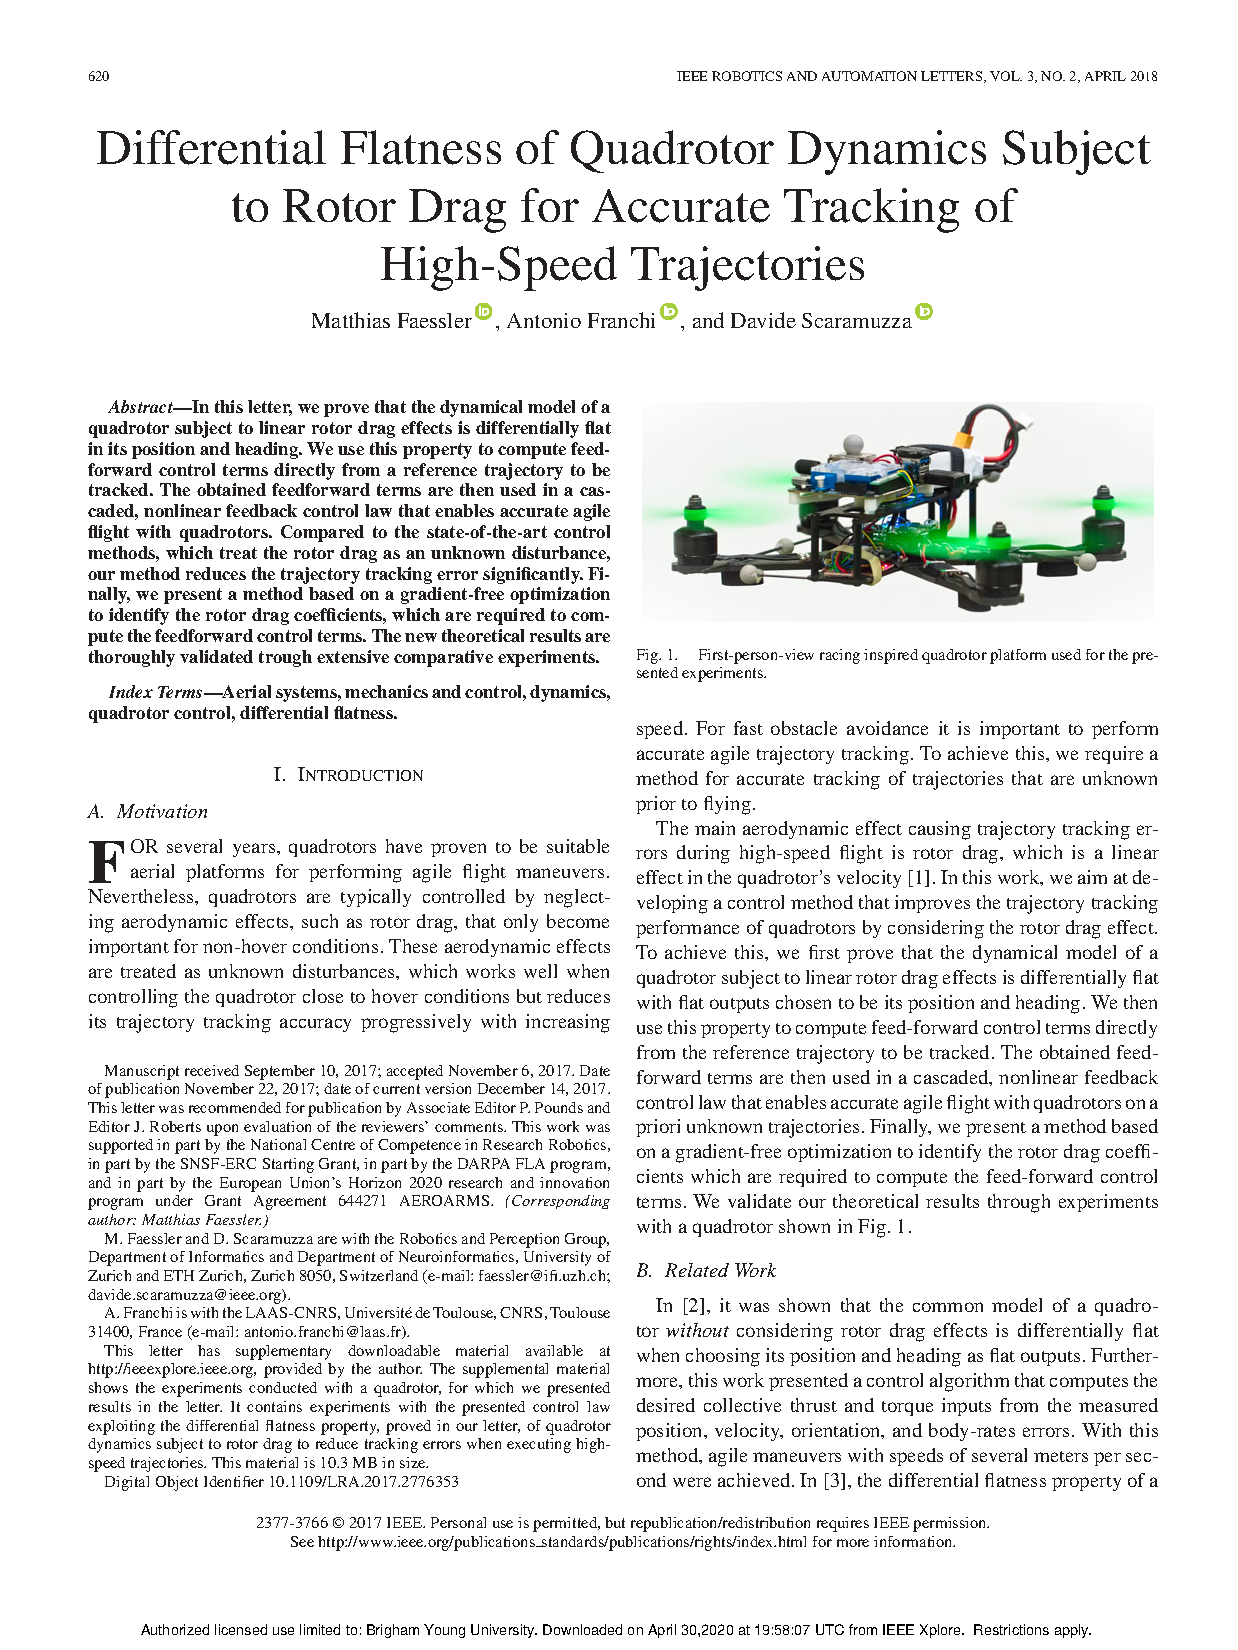
\includepdf[pages=-,scale=.8,pagecommand={}]{chap5_trajectory_planning/papers/FaesslerFranchiScaramuzza18.pdf}




%++++++++++++++++++++++++++++++++++++++++++++++++++++++++++++++
\subsection{Analytic calculation of desired angular velocity}
Author: Jacob Willis

%
%\usepackage[utf8]{inputenc}
%\usepackage{amsmath}
%\usepackage{amssymb}
%\usepackage{graphicx}
%\graphicspath{ {./figs/} }
%
%% \usepackage{theorem}
%\usepackage{amsthm}
%\newtheorem{theorem}{Theorem}
%\newtheorem{property}{Property}
%\def\proof{\hspace{1em}{\it Proof: }}
%\def\endproof{\hspace*{\fill}~$\blacksquare$\par\endtrivlist\unskip}
%
%\newtheorem*{remark}{Remark}
%
%\usepackage[hidelinks]{hyperref}
%\usepackage{color}
%\newcommand{\rwbcomment}[1]{{\color{red} RWB: #1}}
%\newcommand{\jbwcomment}[1]{{\color{blue} JBW: #1}}
%%\usepackage{cite}
%\usepackage{multirow}
%\usepackage[margin=1in]{geometry}
%
%\usepackage{biblatex}
%\addbibresource{bib_willis/references.bib}
%
%%\DeclareMathOperator{\mod}{mod}
%\DeclareMathOperator{\floor}{floor}
%\DeclareMathOperator{\rank}{rank}
%\DeclareMathOperator{\vspan}{span}
%\DeclareMathOperator*{\argmin}{arg min}
%
%\title{\LARGE Analytic Derivative of the Desired Rotation Matrix for Control}
%\author{Jacob Willis}
%
%\begin{document}
%\maketitle

Rather than numerically differentiating $R_d^i$ as described in Section~\ref{sec:numerical_differentiation_of_R}, this section shows how to find the time derivative of $R_d^i$ analytically.
First, recall that
\begin{equation}
	R_d^i = \begin{pmatrix} \mathbf{r}_{1d} & \mathbf{r}_{2d}&  \mathbf{r}_{3d} \end{pmatrix}
\end{equation}
and therefore that
\begin{equation}
	\dot{R}_d^i = \begin{pmatrix} \dot{\mathbf{r}}_{1d} & \dot{\mathbf{r}}_{2d} & \dot{\mathbf{r}}_{3d} \end{pmatrix}.
\end{equation}

To proceed, we need the following two properties.
\begin{property}
	The time derivative of the cross product of two time-dependent vectors $\mathbf{x}$ and $\mathbf{y}$ is
	\begin{equation}
		\label{eq:cross_derivative}
		\frac{d}{dt} (\mathbf{x} \times \mathbf{y}) = \dot{\mathbf{x}} \times \mathbf{y} + \mathbf{x} \times \dot{\mathbf{y}}
	\end{equation}
\end{property}
\proof
This is easiest to see by recalling that $\mathbf{x} \times \mathbf{y} = \mathbf{x}^\wedge \mathbf{y}$ where the result follows from the product rule.
\endproof

\begin{property} \label{prop:derivative_of_normal_vector}
	The time derivative of a normalized vector $\frac{\mathbf{x}}{\|\mathbf{x}\|}$ is
	\begin{equation}
		\label{eq:norm_derivative}
		\frac{d}{dt} \left(\frac{\xbf}{\norm{\xbf}}\right) = \Pi_{\frac{\xbf}{\norm{\xbf}}} \frac{\dot{\xbf}}{\norm{\xbf}},
	\end{equation}
	where $\Pi_{\nbf} \doteq I-\nbf\nbf^\top$ is the projection operator on to the plane orthogonal to the unit vector $\nbf$.
\end{property}
\proof
	By the quotient rule, we have
	\begin{equation}
		\frac{d}{dt} \frac{\mathbf{x}}{\|\mathbf{x}\|} = \frac{\dot{\mathbf{x}} \|\mathbf{x}\| - \mathbf{x} \frac{d}{dt}(\|\mathbf{x}\|)}{\|\mathbf{x}\|^2}.
	\end{equation}
	Now,
	\begin{align}
		\frac{d}{dt} \|\mathbf{x}\| 
		= \frac{d}{dt} \sqrt{\mathbf{x}^\top \mathbf{x}} 
		= \frac{1}{2 \sqrt{\mathbf{x}^\top \mathbf{x}}} (\dot{\mathbf{x}}^\top \mathbf{x} + \mathbf{x}^\top \dot{\mathbf{x}})
		= \frac{\dot{\mathbf{x}}^\top \mathbf{x}}{\|\mathbf{x}\|}
	\end{align}
	Plugging in, we get
	\begin{equation}
		\frac{d}{dt} \frac{\mathbf{x}}{\|\mathbf{x}\|} = \frac{\dot{\mathbf{x}}}{\|\mathbf{x}\|} - \mathbf{x} \frac{\dot{\mathbf{x}}^\top \mathbf{x}}{\|\mathbf{x}\|^3}.
	\end{equation}
	Rearranging gives
	\[
	\frac{d}{dt} \frac{\mathbf{x}}{\|\mathbf{x}\|} =  \left(I-\frac{\xbf}{\norm{\xbf}}\frac{\xbf^\top}{\norm{\xbf}}\right)\frac{\dot{\xbf}}{\norm{\xbf}}.
	\]

\endproof

The third column of the rotation matrix is given by
\begin{equation}
	\mathbf{r}_{3d} = - \frac{\ddot{\mathbf{p}}_d - g \mathbf{e}_3 - K_p \tilde{\mathbf{p}} - K_d \dot{\tilde{\mathbf{p}}}} {\norm{\ddot{\pbf}_d - g \ebf_3 - K_p \tilde{\pbf} - K_d \dot{\tilde{\pbf}}}}.
\end{equation}
Therefore, using the properties above we get that
\[
\dot{\rbf}_{3d} = \Pi_{\rbf_{3d}} \left(\frac{-\dddot{\pbf}_d + K_p \dot{\tilde{\pbf}} + K_d \ddot{\tilde{\pbf}}}{\norm{\ddot{\pbf}_d - g \ebf_3 - K_p \tilde{\pbf} - K_d \dot{\tilde{\pbf}}}}\right).
\]
The second column of the rotation matrix is given by
\[
\rbf_{2d} = \frac{\rbf_{3d}\times\sbf_{\psi_d}}{\norm{\rbf_{3d}\times\sbf_{\psi_d}}},
\]
which implies that
\[
\dot{\rbf}_{2d} = \Pi_{\rbf_{2d}}\left(\frac{\dot{\rbf}_{3d}\times\sbf_{\psi_d}+\dot{\psi}_d\rbf_{3d}\times (-\sin\psi_d,  \cos\psi_d, 0)^\top }{\norm{\rbf_{3d}\times\sbf_{\psi_d}}}\right).
\]
The first column of the rotation matrix is given by
\[
\rbf_{1d} = \rbf_{2d}\times\rbf_{3d},
\]
which implies that
\[
\dot{\rbf}_{1d} = \dot{\rbf}_{2d}\times\rbf_{3d} + \rbf_{2d}\times \dot{\rbf}_{3d}.
\]
The angular velocity can now be calculated as
\[
\omegabf_{d/i}^d(\pbf_d, \dot{\pbf}_d, \ddot{\pbf}_d, \dddot{\pbf}_d, \psi_d, \dot{\psi}_d) = \left[\begin{pmatrix}\rbf_{1d} & \rbf_{2d} & \rbf_{3d}\end{pmatrix}^\top \begin{pmatrix} \dot{\rbf}_{1d} & \dot{\rbf}_{2d} & \dot{\rbf}_{3d} \end{pmatrix}\right]^\vee.
\]





%----------------------------------
\section{An Introduction to b-Spline}


The objective of these notes is to explore spline methods for robotic applications. In general, the position of a robot in Euclidian space can be described by a time parametrized trajectory $\mathbf{p}(t)\in\mathbb{R}^3$, $t\in[a,b]$.  The time parametrized trajectory can be parameterized using a weighted sum of basis function as
\[
\mathbf{p}(t) = \sum_{m=0}^{N} \cbf_m \phi_m(t),
\]
where $\cbf_m\in\mathbb{R}^n$, and $\phi_m(t)$ are a set of basis functions.  For example, the basis functions could be the set of polynomial power function $\phi_m(t) = t^m/m!$, or the set of sinusoidal function $\phi_m(t) = \sin(\frac{2\pi m}{N}t)$.  The disadvantage of both the polynomial power functions and sinusoidal functions is that the basis functions are defined for all $t\in[a,b]$ and so each control points $\mathbf{c}_m$ influences the entire trajectory.  Another disadvantage is that a large number of basis functions may be required to represent complicated trajectories.  

In these notes, we will use B-spline basis functions which have a number of very nice properties that we will explore.  In particular, a {\em B-spline} trajectory has the following form
\[
\mathbf{p}(t) = \sum_{m=0}^{N} \cbf_m b_m^k(t;\mathbf{t}),
\]
where $\cbf_m\in\mathbb{R}^n$ are the control points,  $\mathbf{t}=(\tau_0, \tau_1, \tau_2, \dots, \tau_T)$ are called the knot points where $i<j \implies \tau_i\leq \tau_j$, and $b_m^k(t;\mathbf{t})$ are the B-spline basis functions of order $k$. The spline trajectories will be defined for $t$ in the span of the knot points, i.e., $t\in[\tau_0, \tau_T]$.  

Section~\ref{sec:b-spline-basis-functions} defines the B-spline basis function $b_m^k(t; \mathbf{t})$ and describes some of their properties that will be useful for path planning and for estimation.
Section~...
% overview of other sections

%---------------------------------------------------------------
\subsection{B-Spline Basis Functions}
\label{sec:b-spline-basis-functions}

The B-spline basis function are defined by the recursive formula:
\begin{align}
b_m^1(t; \mathbf{t}) &= \begin{cases} 1 & \text{~if~} \tau_m \leq t \leq \tau_{m+1} \\ 
 									 0 & \text{~otherwise} 
 					   \end{cases} 
	\label{eq:spline_basis_definition_0}\\	
b_m^k(t; \mathbf{t}) &= w_m^k(t; \mathbf{t}) b_m^{k-1}(t; \mathbf{t}) + \left[1-w_{m+1}^k(t; \mathbf{t})\right] b_{m+1}^{k-1}(t; \mathbf{t}),
	\label{eq:spline_basis_definition_k} \\
w_m^k(t; \mathbf{t}) &= \begin{cases}
                      		\frac{t-\tau_m}{\tau_{m+k}-\tau_m}, & \tau_{m+k}\neq \tau_m \\
                      		0, & \text{~otherwise} 
                        \end{cases}.
\end{align}

%+++++++++++++++++++++++++++++++
\par\noindent{\bf First order basis}

For example, if the knot vector is given by
\[
\mathbf{t} = [\tau_0, \tau_1, \tau_2] \defeq [0, 1, 2],
\]
then there are two basis function of order $k=1$ given by
\begin{align*}
b_0^1(t; \mathbf{t}) &= \begin{cases} 1 & \text{~if~} \tau_0 \leq t \leq \tau_1 \\ 
 									 0 & \text{~otherwise} 
 			\end{cases}
\\ 
b_1^1(t; \mathbf{t}) &= \begin{cases} 1 & \text{~if~} \tau_1 \leq t \leq \tau_2 \\ 
 									 0 & \text{~otherwise}
 			\end{cases}
\end{align*}
where $b_0^1(t)$ and $b_1^0=1(t)$ are shown in Figure~\ref{fig:spline_basis_0}.
\begin{figure}[hbt]
  \centering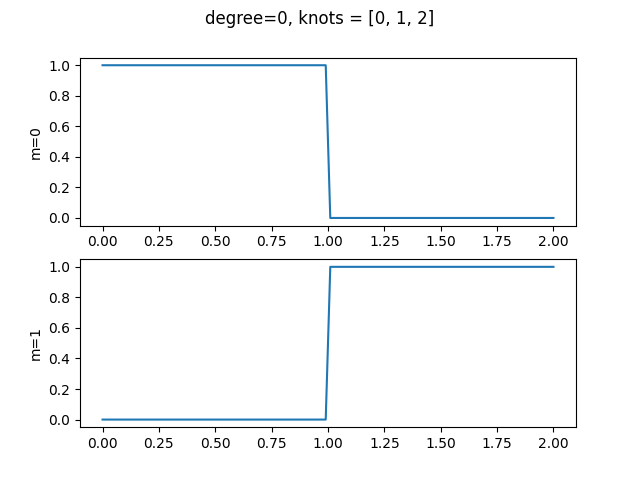
\includegraphics[width=0.5\textwidth]{./chap5_trajectory_planning/figures/spline_basis_0}
  \caption{First order spline basis}
  \label{fig:spline_basis_0}  
\end{figure}
Note that $b_1^1(t; \mathbf{t}) = b_0^1(t-1; \mathbf{t})$, or in other words, all first order basis functions are shifted versions of the central first order basis function $b_0^1(t; \mathbf{t})$.  Additional first order basis function can be defined by expanding the knot vector to $\mathbf{t}=[0, \dots, M]$, where $b_m^1(t; \mathbf{t})= b_0^1(t-m; \mathbf{t})$ for $m\leq M$.

\clearpage


%+++++++++++++++++++++++++++++++
\par\noindent{\bf Second order basis}

If the knot vector is given by
\[
\mathbf{t} = [\tau_0, \tau_1, \tau_2, \tau_3, \tau_4] \defeq [0, 0, 1, 2, 2],
\]
then there are $2k-1=3$ unique basis function of order $k=2$ given by
\begin{align*}
b_0^2(t; \mathbf{t}) &= \frac{t-\tau_0}{\tau_1-\tau_0} b_0^1(t;\mathbf{t}) + \frac{\tau_2-t}{\tau_2-\tau_1}b_1^1(t; \mathbf{t}) 
	= \begin{cases} 0   & \text{~if~} t_0=0 \leq t \leq t_1=0 \\
				    1-t & \text{~if~} t_1=0 \leq t \leq t_2=1 \\ 
 	  \end{cases}
\\ 
b_1^2(t; \mathbf{t}) &= \frac{t-\tau_1}{\tau_2-\tau_1} b_1^1(t;\mathbf{t}) + \frac{\tau_3-t}{\tau_3-\tau_2}b_2^1(t; \mathbf{t})
	= \begin{cases} t & \text{~if~} t_1=0 \leq t \leq t_2=1 \\ 
 									2-t & t_2=1 \leq t \leq t_3=2 \\
 									0 & \text{~otherwise}
 					    \end{cases}
\\ 
b_2^2(t; \mathbf{t}) &= \frac{t-\tau_2}{\tau_3-\tau_2} b_2^1(t;\mathbf{t}) + \frac{\tau_4-t}{\tau_4-\tau_3}b_3^1(t; \mathbf{t})
	= \begin{cases} t-1 & \text{~if~} t_2=1 \leq t \leq t_3=2 \\ 
 					0 & \text{~if~} t_3=2 \leq t \leq t_4=2 \\
 	  \end{cases}
\end{align*}
where $b_0^2(t; \mathbf{t})$, $b_1^2(t; \mathbf{t})$, and $b_2^2(t; \mathbf{t})$ are shown on the left in Figure~\ref{fig:spline_basis_1}.
\begin{figure}[hbt]
  \centering
  	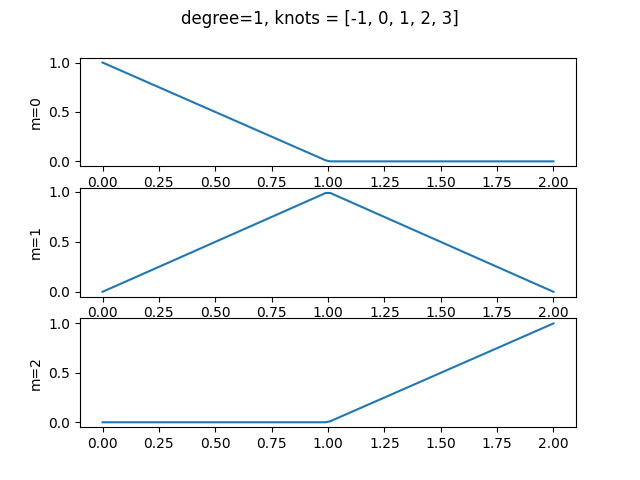
\includegraphics[width=0.45\textwidth]{./chap5_trajectory_planning/figures/spline_basis_1}
  	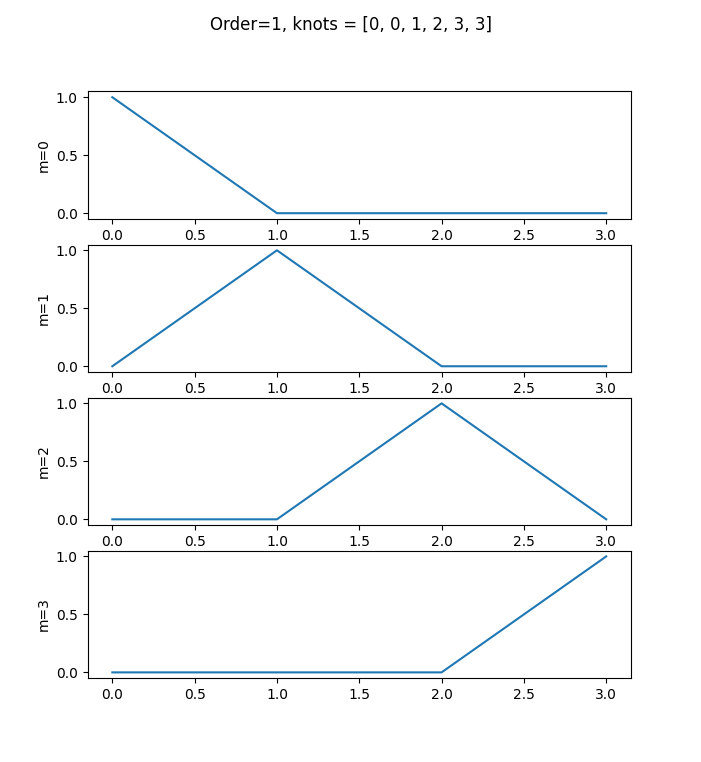
\includegraphics[width=0.45\textwidth]{./chap5_trajectory_planning/figures/spline_basis_1_extra_knot}
  \caption{Second order spline basis}
  \label{fig:spline_basis_1}  
\end{figure}
If the knot vector is expanded by one time unit to
\[
\mathbf{t}' = [\tau_0, \tau_1, \tau_2, \tau_3, \tau_4, \tau_5] \defeq [0, 0, 1, 2, 3, 3],
\]
then there are still only three unique basis vectors, but 
$b_2^2(t; \mathbf{t}')$ is a shifted version $b_1^2(t; \mathbf{t})$ and $b_3^2(t; \mathbf{t}')$ is a shifted version $b_2^2(t; \mathbf{t})$, as shown on the right in Figure~\ref{fig:spline_basis_1}.

\clearpage


%+++++++++++++++++++++++++++++++
\par\noindent{\bf Third order basis}

If the knot vector is given by
\[
\mathbf{t} = [\tau_0, \tau_1, \tau_2, \tau_3, \tau_4, \tau_5, \tau_6, \tau_7, \tau_8] \defeq [0, 0, 0, 1, 2, 3, 3, 3],
\]
then there are $2k-1=5$ unique basis function of order $k=3$ given by
\begin{align*}
b_0^3(t; \mathbf{t}) &= \frac{t-\tau_0}{\tau_2-\tau_0} b_0^2(t;\mathbf{t}) + \frac{\tau_3-t}{\tau_3-\tau_1}b_1^2(t; \mathbf{t}) 
	= \begin{cases} (1-t)^2   & \text{~if~} 0 \leq t \leq 1 \\
				    0 & \text{~otherwise~}  \\ 
 	  \end{cases}
\\ 
b_1^3(t; \mathbf{t}) &= \frac{t-\tau_1}{\tau_3-\tau_1} b_1^2(t;\mathbf{t}) + \frac{\tau_4-t}{\tau_4-\tau_2}b_2^2(t; \mathbf{t})
	= \begin{cases} t(2-\frac{3}{2}t) & \text{~if~} 0 \leq t \leq 1 \\ 
 									\frac{(2-t)^2}{2} & 1 \leq t \leq 2 \\
 									0 & \text{~otherwise}
 					    \end{cases}
\\ 
b_2^3(t; \mathbf{t}) &= \frac{t-\tau_2}{\tau_4-\tau_2} b_2^2(t;\mathbf{t}) + \frac{\tau_5-t}{\tau_5-\tau_3}b_3^2(t; \mathbf{t})
	= \begin{cases} \frac{t^2}{2} & \text{~if~} 0 \leq t \leq 1 \\ 
 					-\frac{3}{2}t^2 + \frac{7}{2}t - \frac{3}{2} & \text{~if~} 1 \leq t \leq 2 \\
 					\frac{(3-t)^2}{2} & \text{~if~} 2 \leq t \leq 3 \\
 					0 & \text{~otherwise}
 	  \end{cases}
\\ 
b_3^3(t; \mathbf{t}) &= \frac{t-\tau_2}{\tau_4-\tau_2} b_2^2(t;\mathbf{t}) + \frac{\tau_5-t}{\tau_5-\tau_3}b_3^2(t; \mathbf{t})
	= \begin{cases} \frac{(t-1)^2}{2} & \text{~if~} 1 \leq t \leq 2 \\ 
 					-\frac{3}{2}t^2 + \frac{15}{2}t-\frac{15}{2} & \text{~if~} 2 \leq t \leq 3 \\
 					0 & \text{~otherwise}
 	  \end{cases}
\\ 
b_4^3(t; \mathbf{t}) &= \frac{t-\tau_2}{\tau_4-\tau_2} b_2^2(t;\mathbf{t}) + \frac{\tau_5-t}{\tau_5-\tau_3}b_3^2(t; \mathbf{t})
	= \begin{cases} (t-2)^2 & \text{~if~} 2 \leq t \leq 3 \\ 
 					0 & \text{~otherwise}
 	  \end{cases}.	   	  
\end{align*}
The the unique third order basis function are shown on the left in Figure~\ref{fig:spline_basis_2}.
\begin{figure}[hbt]
  \centering
  	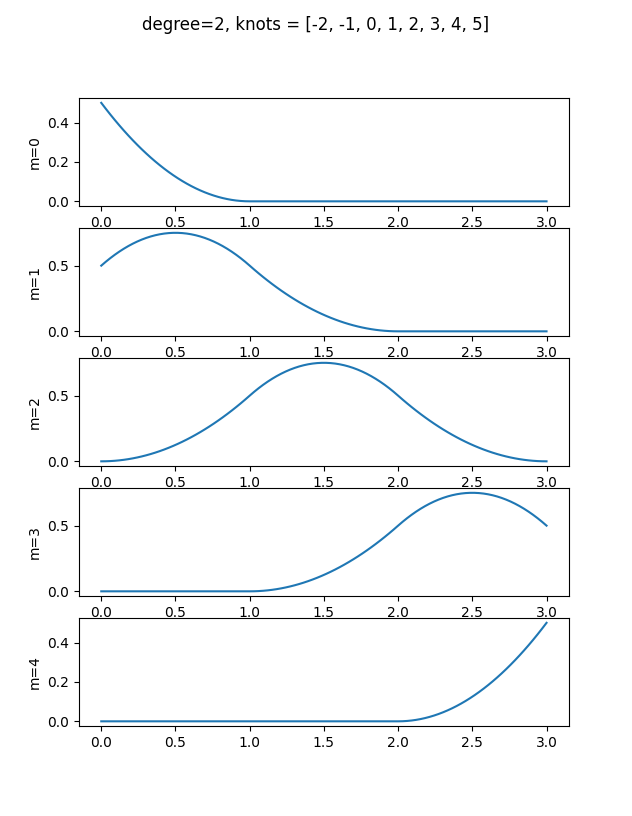
\includegraphics[width=0.45\textwidth]{./chap5_trajectory_planning/figures/spline_basis_2}
  	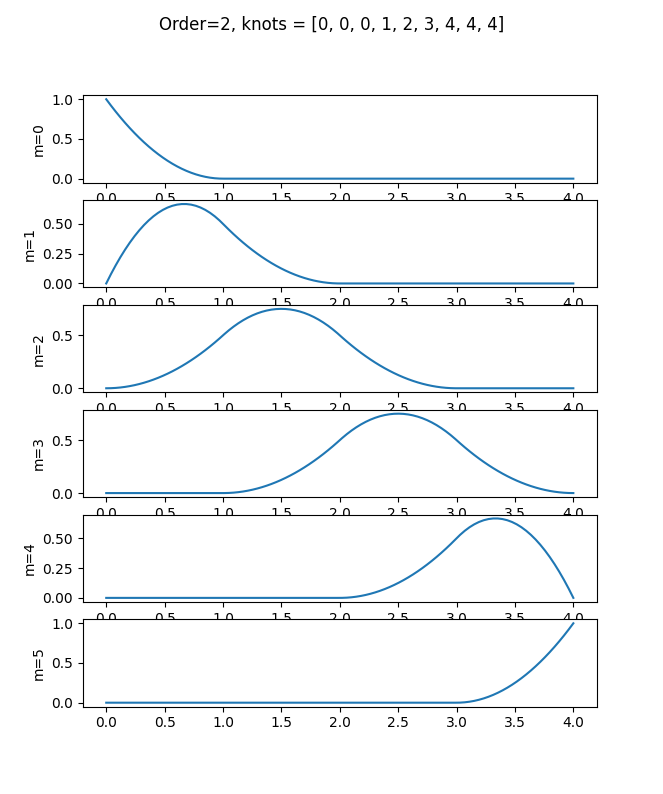
\includegraphics[width=0.45\textwidth]{./chap5_trajectory_planning/figures/spline_basis_2_extra_knot}
  \caption{Third order spline basis}
  \label{fig:spline_basis_2}  
\end{figure}
Expanding the knot vector by one time unit to 
\[
\mathbf{t}' = [\tau_0, \tau_1, \tau_2, \tau_3, \tau_4, \tau_5] \defeq [0, 0, 0, 1, 2, 3, 4, 4, 4],
\]
still results in $2k-1$ unique basis vectors, but $b_3^3(t; \mathbf{t}')$ is a right-shifted version of $b_2^3(t; \mathbf{t})$, and $b_4^3(t; \mathbf{t}')$ and $b_5^3(t; \mathbf{t})$ are a right-shifted versions of $b_3^3(t; \mathbf{t}')$ and $b_4^3(t; \mathbf{t})$, as shown on the right in Figure~\ref{fig:spline_basis_2}.

Similarly, the unique fourth order and ninth order basis functions are shown in Figures~\ref{fig:spline_basis_3} and~\ref{fig:spline_basis_8} respectively.

\begin{figure}[hbt]
  \centering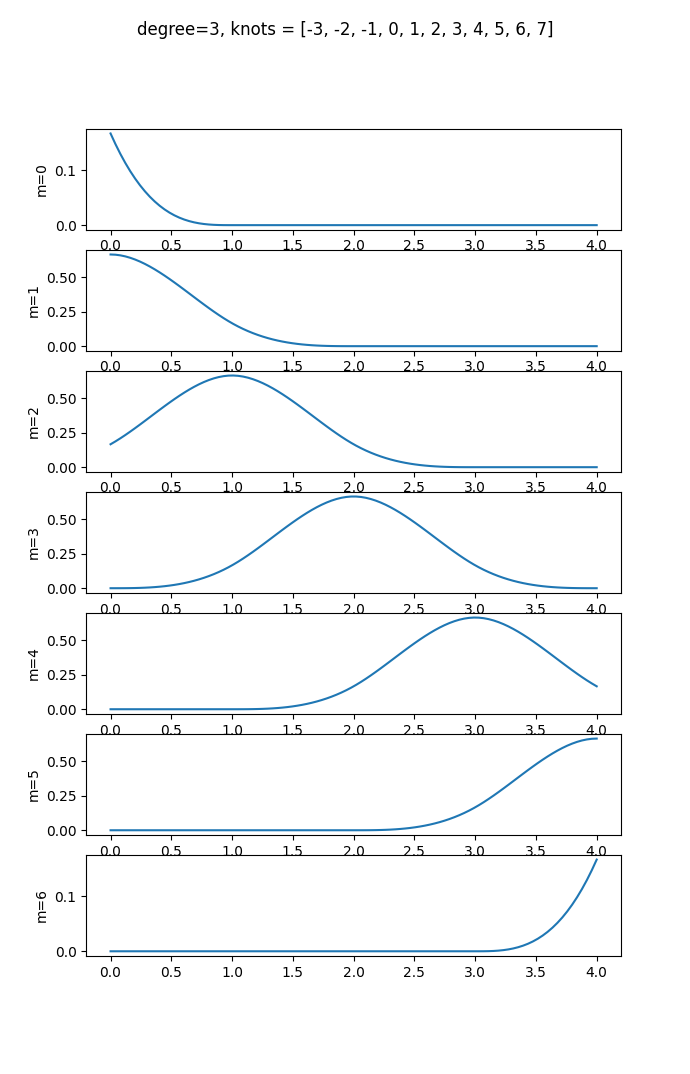
\includegraphics[width=0.99\textwidth]{./chap5_trajectory_planning/figures/spline_basis_3}
  \caption{Fourth order spline basis}
  \label{fig:spline_basis_3}  
\end{figure}

\begin{figure}[hbt]
  \centering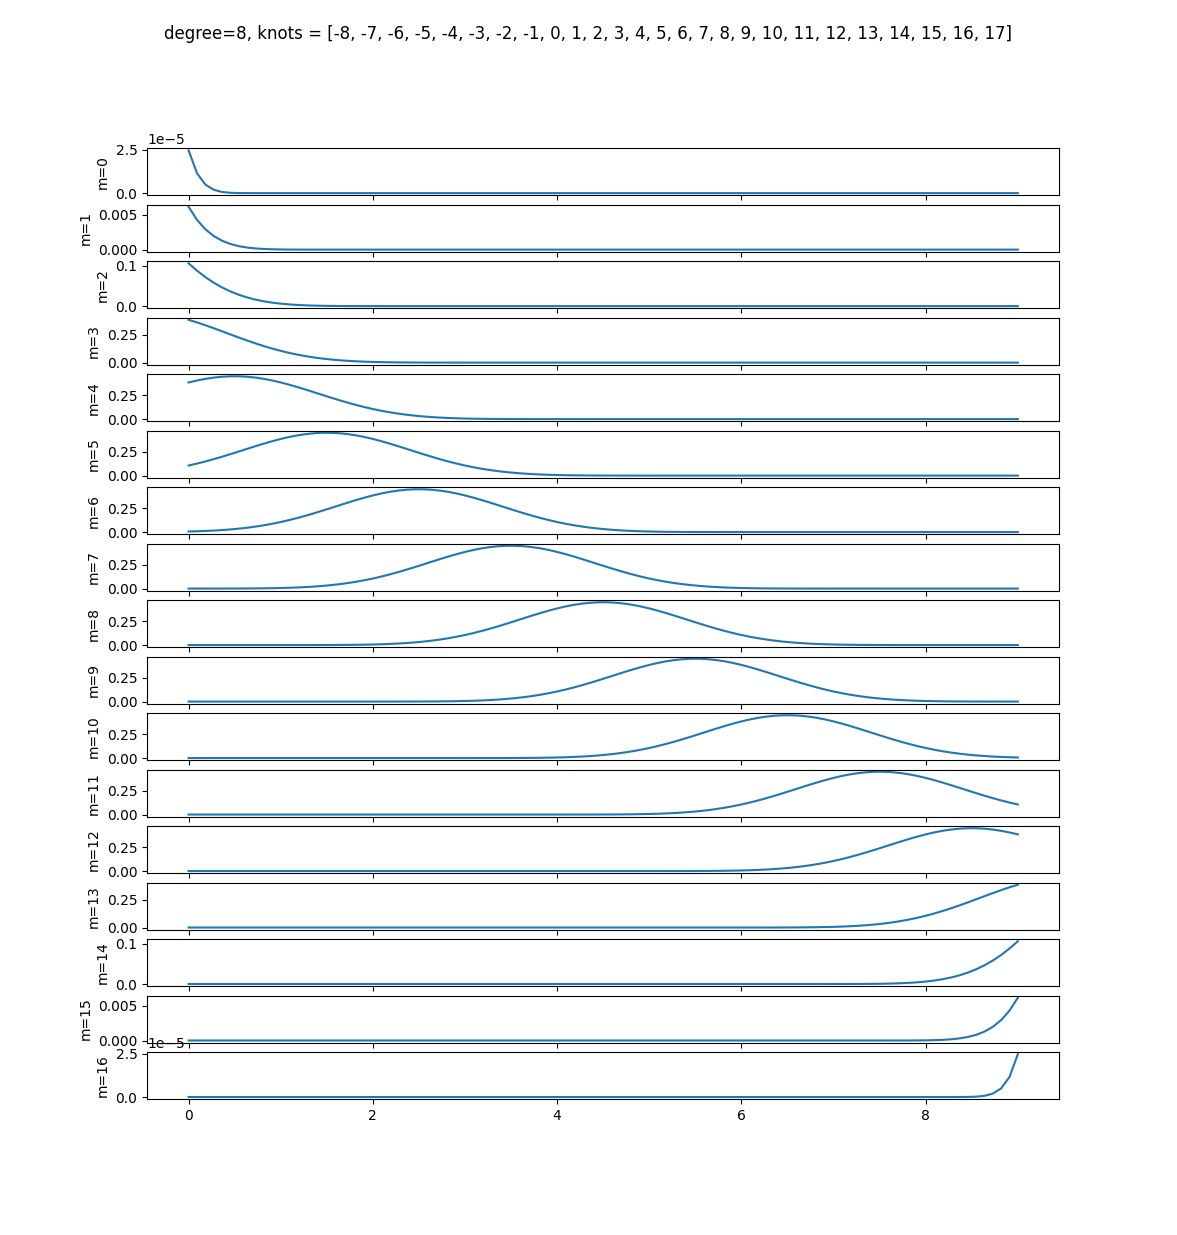
\includegraphics[width=0.99\textwidth]{./chap5_trajectory_planning/figures/spline_basis_8}
  \caption{Ninth order spline basis}
  \label{fig:spline_basis_8}  
\end{figure}

\clearpage

%---------------------------------------------------------------
\par\noindent{\bf Shift and Scale Invariance of the Knot Sequence}

\begin{lemma} \label{lem:basis_are_shift_invariant}
Given an arbitrary knot sequence
\[
\mathbf{t} = [\tau_0, \tau_1, \dots \tau_T],
\]
an arbitrary time shift $\Delta$, and the one-sequenc $\mathbf{1}\defeq[1, 1, \dots, 1]$, the B-spline basis functions are shift invariant in the sense that
if 
\[
\mathbf{t} + \Delta\mathbf{1} = [\tau_0+\Delta, \tau_1+\Delta, \dots \tau_T+\Delta]
\]
then
\[
b_j^k(t; \mathbf{t}+\Delta\mathbf{1}) = b_j^k(t-\Delta; \mathbf{t}),
\]
i.e., shifting the knot sequence forward in time is identical to shifting the original B-spline forward in time.
\end{lemma}
\begin{proof}
When the order is $k=1$, then equation~\eqref{eq:spline_basis_definition_0} gives
\begin{align*}
	b_j^1(t; \mathbf{t}+\Delta\mathbf{1}) &= \begin{cases} 1 & \text{~if~} \tau_j+\Delta \leq t \leq \tau_{j+1}+\Delta \\ 
 									 				   0 & \text{~otherwise} 
 					   					 \end{cases} \\
 					   				   &= \begin{cases} 1 & \text{~if~} \tau_j \leq t-\Delta \leq \tau_{j+1} \\ 
 									 				   0 & \text{~otherwise} 
 					   					 \end{cases} \\ 	
 					   				   &= b_j^1(t-\Delta; \mathbf{t}).
\end{align*}
Assuming that the statement holds when the order is $k-1\geq 0$, we get from 
Equation~\eqref{eq:spline_basis_definition_k} that
\begin{align*}
b_j^k(t; \mathbf{t}+\Delta\mathbf{1}) &= \frac{t-\tau_j-\Delta}{\tau_{j+k}+\Delta-
\tau_j-\Delta} b_j^{k-1}(t; \mathbf{t}+\Delta\mathbf{1}) + \frac{\tau_{j+k+1}+\Delta-t}{\tau_{j+k+1}+\Delta-\tau_{j+1}-\Delta} b_{j+1}^{k-1}(t; \mathbf{t}+\Delta\mathbf{1}) \\
&= \frac{(t-\Delta)-\tau_j}{\tau_{j+k}-
\tau_j} b_j^{k-1}(t-\Delta; \mathbf{t}) + \frac{\tau_{j+k+1}-(t-\Delta)}{\tau_{j+k+1}-\tau_{j+1}} b_{j+1}^{k-1}(t-\Delta; \mathbf{t}) \\
&= b_j^k(t-\Delta; \mathbf{t}).
\end{align*}
The proof therefore follows by induction.
\end{proof}


\begin{lemma}\label{lem:bases_are_scale_invariant}
Given an arbitrary knot sequence
\[
\mathbf{t} = [\tau_0, \tau_1, \dots \tau_T]
\]
and an arbitrary scaling constant $\alpha\in\mathbb{R}$, the B-spline basis functions are scale invariant in the sense that
if 
\[
\alpha\mathbf{t} = [\alpha\tau_0, \alpha\tau_1, \dots \alpha\tau_T]
\]
then
\[
b_j^k(t; \alpha\mathbf{t}) = b_j^k(t/\alpha; \mathbf{t}),
\]
i.e., scaling the knot sequence by $\alpha$ is identical to time scaling the original B-spline by $\frac{1}{\alpha}$.
\end{lemma}
\begin{proof}
When the order is $k=1$, then equation~\eqref{eq:spline_basis_definition_0} gives
\begin{align*}
	b_j^1(t; \alpha\mathbf{t}) &= \begin{cases} 1 & \text{~if~} \alpha\tau_j \leq t \leq \alpha\tau_{j+1} \\ 
 									 				   0 & \text{~otherwise} 
 					   					 \end{cases} \\
 					   				   &= \begin{cases} 1 & \text{~if~} \tau_j \leq \frac{t}{\alpha} \leq \tau_{j+1} \\ 
 									 				   0 & \text{~otherwise} 
 					   					 \end{cases} \\ 	
 					   				   &= b_j^1(t/\alpha; \mathbf{t}).
\end{align*}
Assuming that the statement holds when the order is $k-1\geq 0$, we get from 
Equation~\eqref{eq:spline_basis_definition_k} that
\begin{align*}
b_j^k(t; \alpha\mathbf{t}) &= \frac{t-\alpha\tau_j}{\alpha\tau_{j+k}-
\alpha\tau_j} b_j^{k-1}(t; \alpha\mathbf{t}) + \frac{\alpha\tau_{j+k+1}-t}{\alpha\tau_{j+k+1}-\alpha\tau_{j+1}} b_{j+1}^{k-1}(t; \alpha\mathbf{t}) \\
&= \frac{(t/\alpha)-\tau_j}{\tau_{j+k}-
\tau_j} b_j^{k-1}(t/\alpha; \mathbf{t}) + \frac{\tau_{j+k+1}-(t/\alpha)}{\tau_{j+k+1}-\tau_{j+1}} b_{j+1}^{k-1}(t/\alpha; \mathbf{t}) \\
&= b_j^k(t/\alpha; \mathbf{t}).
\end{align*}
The proof therefore follows by induction.
\end{proof}


%---------------------------------------------------------------
\subsection{Uniform B-Splines}

In the previous section we saw that there is a relationship between the knot point vector $\mathbf{t}$ and the basis functions.  We say that the knot vector $\mathbf{t}$ is {\em uniform} if the knot values are equally spaced, i.e., it has form
\begin{multline*}
\mathbf{t} = [\underbrace{\tau_0-(k-1)\Delta, \dots, \tau_0-\Delta,}_{(k-1)-terms} \\
			 \underbrace{\tau_0, \tau_0+\Delta, \tau_0+2\Delta, \dots, \tau_0+M\Delta,}_{M+1-terms} \\
			 \underbrace{\tau_0+(M+1)\Delta, \dots, \tau_0+(M+k-1)\Delta}_{(k-1)-terms}],	
\end{multline*}
where $\Delta>0$ and $M\geq k$.  
For example, the following knot vectors are uniform:
\begin{align*}
	(t_0=0, k=3, \Delta=1, M=3):\quad & \mathbf{t} = [-2, -1, \vdots~ 0, 1, 2, 3, \vdots~ 4, 5] \\
	(t_0=-3, k=4, \Delta=1, M=5):\quad & \mathbf{t} = [-6, -5, -4,\vdots~  -3, -2, -1, 0, 1, 2, \vdots~ 3, 4, 5] \\
	(t_0=0, k=4, \Delta=\frac{1}{5}, M=5):\quad & \mathbf{t} = [-\frac{3}{5}, -\frac{2}{5}, -\frac{1}{5}, \vdots~  0, \frac{1}{5}, \frac{2}{5}, \frac{3}{5}, \frac{4}{5}, 1, \vdots~  \frac{6}{5}, \frac{7}{5}, \frac{8}{5}].	
\end{align*}

 We say that the knot vector $\bar{\mathbf{t}}$ is {\em uniform and clamped} (the overbar is used to denote clamped) if the knot values are equally spaced and the first and last $(k-1)$-terms are repeated, i.e., it has form
\begin{multline*}
\bar{\mathbf{t}} = [\underbrace{\tau_0, \tau_0, \dots, \tau_0,}_{(k-1)-terms} \\
			 \underbrace{\tau_0, \tau_0+\Delta, \tau_0+2\Delta, \dots, \tau_0+M\Delta,}_{M+1-terms} \\
			 \underbrace{\tau_0+M\Delta, \dots, \tau_0+M\Delta}_{(k-1)-terms}],	
\end{multline*}
where $\Delta>0$ and $M\geq k$.  

For example, the following knot vectors are clamped and uniform:
\begin{align*}
	(t_0=0, k=3, \Delta=1, M=3):\quad & \bar{\mathbf{t}} = [0, 0, \vdots~ 0, 1, 2, 3, \vdots~ 3, 3] \\
	(t_0=-3, k=4, \Delta=1, M=5):\quad & \bar{\mathbf{t}} = [-3, -3, -3, \vdots~ -3, -2, -1, 0, 1, 2, \vdots~ 2, 2, 2] \\
	(t_0=0, k=4, \Delta=\frac{1}{5}, M=5):\quad & \bar{\mathbf{t}} = [0, 0, 0, \vdots~ 0, \frac{1}{5}, \frac{2}{5}, \frac{3}{5}, \frac{4}{5}, 1, \vdots~ 1, 1, 1].	
\end{align*}
Similarly, the knot vectors shown in Figures~\ref{fig:spline_basis_0}, \ref{fig:spline_basis_1}, \ref{fig:spline_basis_2}, \ref{fig:spline_basis_3}, and~\ref{fig:spline_basis_8} are all clamped and uniform.  

The length of uniform, and uniform and clamped knot vectors is 
\[
\text{length}(\mathbf{t}) = M+1 + 2(k-1) = M+2k-1,
\]
and, in both cases, the time interval of interest is $t\in[t_0, t_0+M\Delta$, where there are $M$ evenly spaced time intervals. 

B-splines associated with uniform knot vectors are called uniform b-splines, and they are only valid on the time interval $t\in[t_0, t_0+M\Delta]$, similarly B-splines associated with uniform and clamped knot vectors are called uniform and clamped b-splines, and they are also only valid on the time interval $t\in[t_0, t_0+M\Delta]$.

In the rest of this tutorial, we will focus on the knot vectors
\begin{align}
	\mathbf{t}^k_M &\defeq [-(k-1), \dots, -1, 0, 1, 2, \dots, M, M+1, \dots, M+k-1],
		\label{eq:knot_vector_t_M} \\ 
	\bar{\mathbf{t}}^k_M &\defeq [\underbrace{0, 0, \dots, 0}_{(k-1)-\text{terms}}, 0, 1, 2, \dots, M, \underbrace{M, \dots, M}_{(k-1)-\text{terms}}], 
	\label{eq:knot_vector_tbar_M}
\end{align}
and use Lemmas~\ref{lem:basis_are_shift_invariant} and~\ref{lem:bases_are_scale_invariant} to adapt the results to any desired time interval by shifting and scaling.

There are several important properties of the B-spline basis functions for uniform and clamped knot vectors, which we will lay out in the next several lemmas.

\begin{lemma} \label{lem:shifted_central_basis}
Let $\mathbf{t}_M^k$ be the uniform knot vector defined in Equation~\eqref{eq:knot_vector_t_M} with $M\geq k$, then the basis function $b_k^{k-1}(t; \mathbf{t}_M^k)$ plays a central role in the sense that
\[
	b_{k-1+m}^{k}(t; \mathbf{t}_M^k) = b_{k-1}^k(t-m; \mathbf{t}_M^k), \qquad m=-k, \dots, M-1.
\]
\end{lemma}
\begin{proof}
From Equation~\eqref{eq:spline_basis_definition_0} we give that
\begin{align*}
	b_m^1(t; \mathbf{t}_M^k) &= \begin{cases} 1 & \text{~if~} m \leq t \leq m+1 \\ 
 									 		  0 & \text{~otherwise} 
 					   			\end{cases} 
 					   		\\
 					   		 &= \begin{cases} 1 & \text{~if~} 0 \leq t-m \leq 1 \\ 
 									 		  0 & \text{~otherwise} 
 					   			\end{cases} 
 					   		\\
 					   		&= b_0^1(t-m; \mathbf{t}_M^k).
\end{align*}
Suppose that $b_{k-2+m}^{k-1}(t; \mathbf{t}_M^k) = b_{k-2}^{k-1}(t-m; \mathbf{t}_M^k)$, then
\begin{align*}
b_{k-1+m}^{k}(t; \mathbf{t}_M^k) 
	&= \frac{t-(k+m)}{m+2k-(m+k)} b_{k-1+m}^{k-1}(t; \mathbf{t}_M^k) + \frac{m+2k+1-t}{m+2k+1-(m+k+1)} b_{k+m}^{k-1}(t; \mathbf{t}_M^k),
	\\	
	&= \frac{(t-m)-k)}{k} b_{k-1}^{k-1}(t-m; \mathbf{t}_M^k) + \frac{2k+1-(t-m)}{k} b_{k1}^{k-1}(t-m; \mathbf{t}_M^k),
	\\
	&= b_{k-1}^k(t-m; \mathbf{t}_M^k).
\end{align*}
Therefore, the lemma holds by induction.
\end{proof}



\begin{lemma} \label{lem:nonzero_basis_vectors}
	Let $\mathbf{t}_M^k$ be a uniform clamped knot vector defined in Equation~\eqref{eq:knot_vector_t_M} with $M\geq k$.
	Then there are exactly $M+k-1$ non-zero basis function of order $k$, namely $b_m^k(t;\mathbf{t}_M^k)$, $m=0, \dots, M+k-1$.
	Furthermore, the basis of support for $b_m^k(t;\mathbf{t}_M^k)$, i.e., the time interval where $b_m^k(t;\mathbf{t}_M^k)$ is non-zero is given by
		\[
				b_m^k(t;\mathbf{t}_M^k) \neq 0 
				\quad \text{~if~} \quad
				\begin{cases}
				t \in [0, m+1] & 0\leq m \leq k-1 \\
				t \in [m-k+1, m+1] & k \leq m \leq M-1 \\
				t \in [m-k+1, M] & M \leq m \leq M+k-2
				\end{cases}.
		\]	
\end{lemma}
\begin{proof}  The proof follows from a careful, but straight-forward accounting using Equations~\eqref{eq:spline_basis_definition_0} and~\eqref{eq:spline_basis_definition_k}.	
\end{proof}

A graphical depiction of the region of support for the set of basis functions $\{b_m^k(t;\mathbf{t}_M^k)\}_{m=0}^{M+k-2}$ is shown in Figure~\ref{fig:region_of_support} for $k=4$ and $M=8$.
\begin{figure}[hbt]
  \centering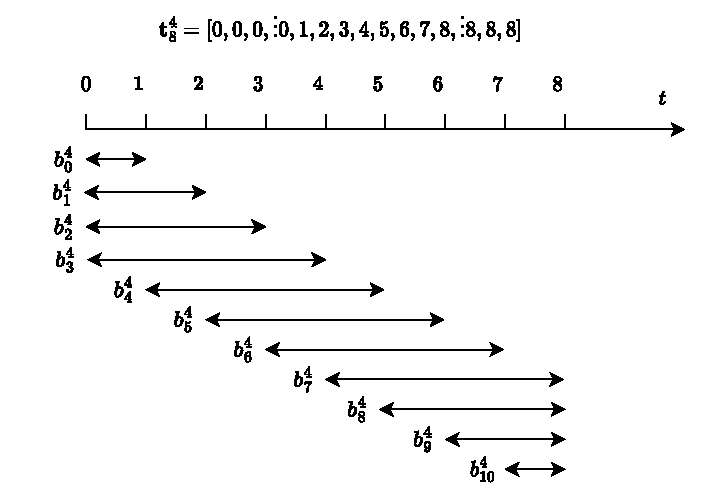
\includegraphics[width=0.99\textwidth]{./chap5_trajectory_planning/figures/region_of_support}
  \caption{Region of support for the B-spline basis functions of order $k=4$ with knot vector $\mathbf{t}_8^4$.}
  \label{fig:region_of_support}  
\end{figure}

\begin{lemma} \label{lem:basis_vectors_sum_to_1}
	Let $\mathbf{t}_M^k$ be a uniform clamped knot vector defined in Equation~\eqref{eq:knot_vector_t_M} with $M\geq k$. For any instant of time $t\in[0,M]$, the basis vectors at that time sum to unity, i.e., for $t\in[0, M]$,
	\[
	\sum_{m=0}^{M+k-2} b_m^k(t; \mathbf{t}_M^k) = 1.
	\]
\end{lemma}
\begin{proof}  The proof again follows from a careful, but straight-forward accounting using Equations~\eqref{eq:spline_basis_definition_0} and~\eqref{eq:spline_basis_definition_k}.	
\end{proof}

\begin{definition}
Let $\{\cbf_0, \cbf_1, \dots, \cbf_{M+k-2}\}$ be a set of control point vectors in $\mathbb{R}^n$, and let $\mathbf{t}_M^k$ be a clamped and uniform knot vector, then the function 
\begin{equation}\label{eq:clamped_uniform_spline}
\mathbf{p}(t) = \sum_{m=0}^{M+k-2} \cbf_m b_m^k(t; \mathbf{t}_M^k), \qquad t\in[0, M]
\end{equation}
is said to be a $k^{th}$ order clamped and uniform B-spline. 
\end{definition}

One of the most important properties of B-splines is the so-called finite-support property, which states that at any instant of time, only a few control points influence the B-spline.  This property is formalized in the following lemma.
\begin{lemma}\label{lem:finite_num_control_points}
	Let $\mathbf{t}_M^k$ be a uniform clamped knot vector defined in Equation~\eqref{eq:knot_vector_t_M} with $M\geq k$. If $0\leq j < M$ is an integer, then for any instant of time $t\in[j, j+1]\subset [0, M]$ we have that
	\[
	\mathbf{p}(t) = \sum_{m=0}^{M+k-2} \cbf_m b_m^k(t; \mathbf{t}_M^k) = \sum_{m=j}^{j+k-1} \cbf_m b_m^k(t; \mathbf{t}_M^k).
	\]
	In other words, over the interval $t\in[j, j+1]$ there are only $k$ control points that influence $\mathbf{p}(t)$, namely
	$\{\cbf_j, \dots, \cbf_{j+k-1}\}$.
\end{lemma}
\begin{proof}
The proof follows directly from Lemma~\ref{lem:nonzero_basis_vectors}.	
\end{proof}



Another important property of B-splines, is that the spline $\mathbf{p}(t)$ is contained in the convex hull of its supporting control points.  
\begin{definition}
We say that the vector $\xbf$ is in the convex hull of the vectors $\{\mathbf{q}_1, \dots, \mathbf{q}_n\}$ if 
\[
\xbf = \sum_{j=1}^n \alpha_j \mathbf{q}_j, \qquad \text{where} \qquad \sum_{j=1}^n \alpha_j = 1.
\]	
\end{definition}

\begin{lemma}\label{lem:spline_in_convex_hull}
	Let $\mathbf{t}_M^k$ be a uniform or uniform clamped knot vector defined in Equation~\eqref{eq:knot_vector_t_M} with $M\geq k$. If $0\leq j < M$ is an integer, then for any instant of time $t\in[j, j+1]\subset [0, M]$ we have that the B-spline
	\[
	\mathbf{p}(t) = \sum_{m=0}^{M+k-2} \cbf_m b_m^k(t; \mathbf{t}_M^k) = \sum_{m=j}^{j+k-1} \cbf_m b_m^k(t; \mathbf{t}_M^k)
	\]
	is in the convex hull of the control points $\{\cbf_j, \dots, \cbf_{j+k-1}\}$.
\end{lemma}
\begin{proof}
	The lemma follows from Lemma~\ref{lem:basis_vectors_sum_to_1} and~\ref{lem:finite_num_control_points}.
\end{proof}
Lemma~\ref{lem:spline_in_convex_hull} is an important result for path planning since we can guarantee collision-free paths by simply checking that the convex hull of control points is collision free.


To simplify notation we will stack the basis function in a vector as
\begin{equation}\label{eq:basis_vector}
\bbf_M^k(t) \defeq \begin{pmatrix} b_0^k(t;\mathbf{t}_M^k) \\ b_1^k(t;\mathbf{t}_M^k) \\ \vdots \\ b_{M+k-2}^k(t;\mathbf{t}_M^k) \end{pmatrix}, 
\end{equation}
and the control points as a matrix 
\[
\Cbf = \begin{pmatrix} \cbf_0 & \cbf_1 & \dots & \cbf_{M+k-2} \end{pmatrix}
\]
allowing Equation~\eqref{eq:clamped_uniform_spline} to be written as
\[
\mathbf{p}(t) = \Cbf \bbf_M^k(t), \qquad t\in[0, M].
\]
Given the shift and scale invariance of the B-spline basis functions, $\mathbf{p}(t)$ can be shifted and scaled to represent functions over arbitrary finite time intervals.

%For parameterized paths $\mathbf{p}(\sigma)$, where the path parameter $\sigma\in[0,1]$ we set the knot vector as $\frac{1}{M}\mathbf{t}_{M}^k$
%and the parameterized B-spline is given by
%\[
%\mathbf{p}(\sigma) = \Cbf \bbf_M^k(\sigma; \frac{1}{M}\mathbf{t}_{M}^k), \qquad \sigma\in[0, 1].
%\]
%Abusing notation, we will use $\bbf_M^k(\sigma)$ to mean $\bbf_M^k(\sigma; \frac{1}{M}\mathbf{t}_{M}^k)$, and parameterized paths with always be defined for $\sigma\in[0,1]$

%---------------------------------------------------------
\par\noindent{\bf SciPy BSpline library}
The SciPy library has a B-spline library.  

The following commands will create a cubic spline.
\begin{lstlisting}
import numpy as np
from scipy.interpolate import BSpline
	
	
def uniform_clamped_knots(k, M, t0=np.inf, tf=np.inf):
    # k is the order, M is the number of time intervals
    knots = [0] * k + list(range(0, M + 1)) + [M] * k
    knots = np.asarray(knots)  # convert knots to an NP array
    if t0 != np.inf:
        if (tf != np.inf) & (tf > t0):
            knots = (tf-t0)/M * knots
        knots = knots + t0
    return knots	

t0 = 1 # initial time
tf = 5 # final time
k = 3  # spline order
M = 3  # number of time intervals
knots = uniform_clamped_knots(k=order, M=M, t0=t0, tf=tf)
# need M+k control points
ctrl_pts = np.array([[0, 0, 0],  
                     [0, 1, 0],
                     [0, 0, 1],
                     [0, 1, 1],
                     [1, 1, 0],
                     [1, 1, 1]])
spl = BSpline(t=knots, c=ctrl_pts, k=order)
plot_spline(spl)
\end{lstlisting}

Where {\tt plot\_spline} is given below.
\begin{lstlisting}
from math import ceil
from scipy.interpolate import BSpline
import matplotlib.pyplot as plt

def plot_spline(spl):
    t0 = spl.t[0]  # first knot is t0
    tf = spl.t[-1]  # last knot is tf
    # number of points in time vector so spacing is 0.01
    N = ceil((tf - t0)/0.01)
    t = np.linspace(t0, tf, N)  # time vector
    position = spl(t)
    # 3D trajectory plot
    fig = plt.figure(1)
    ax = fig.add_subplot(111, projection='3d')
    # plot control points (convert YX(-Z) -> NED)
    ax.plot(spl.c[:, 1], spl.c[:, 0], -spl.c[:, 2],
            '-o', label='control points')
    # plot spline (convert YX(-Z) -> NED)
    ax.plot(position[:, 1], position[:, 0], -position[:, 2],
            'b', label='spline')
    ax.legend()
    ax.set_xlabel('x', fontsize=16, rotation=0)
    ax.set_ylabel('y', fontsize=16, rotation=0)
    ax.set_zlabel('z', fontsize=16, rotation=0)
    #ax.set_xlim3d([-10, 10])
    plt.show()
\end{lstlisting}

The resulting spline is shown in Figure~\ref{fig:example_spline_curve}.
\begin{figure}[hbt]
  \centering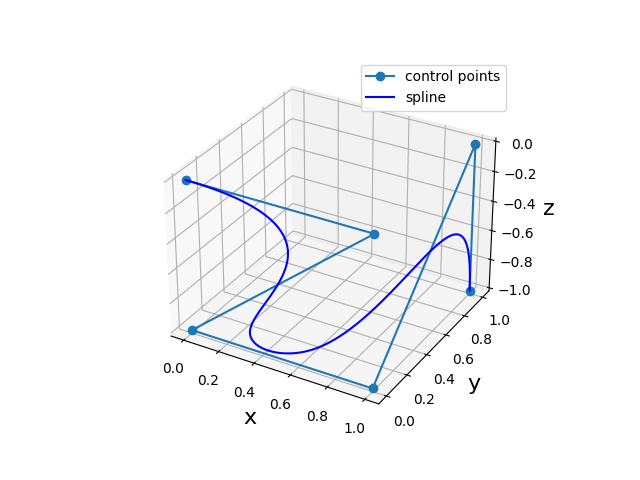
\includegraphics[width=0.5\textwidth]{./chap5_trajectory_planning/figures/example_spline_curve}
  \caption{Example spline curve}
  \label{fig:example_spline_curve}  
\end{figure}

%+++++++++++++++++++++++++++++++
\subsection{Derivatives of B-splines}

We begin this section by noting that the basis functions and the knot vector do not have to be of the same order.  In fact, if the knot vector has higher order than the basis functions, then the first several basis functions will simply be zero.  
For example, let $\mathbf{t}_3^3 = [0, 0\vdots, 0, 1, 2, 3, \vdots 3, 3]$, then from Equation~\eqref{eq:spline_basis_definition_0} $b_0^1(t; \mathbf{t}_3^3)$, $b_1^1(t; \mathbf{t}_3^3)$, $b_5^1(t; \mathbf{t}_3^3)$, $b_1^1(t; \mathbf{t}_3^3)$, and $b_5^2(t; \mathbf{t}_3^3)$ are equal to zero since the knot intervals in the denominator for those functions are zero.  The remaining basis functions are shown in Figure~\ref{fig:shifting_property}.
\begin{figure}[hbt]
  \centering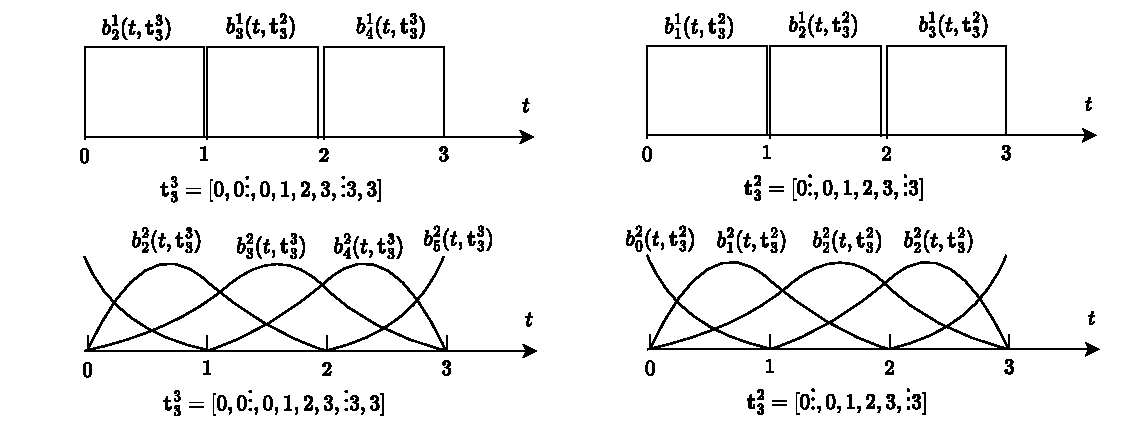
\includegraphics[width=0.99\textwidth]{./chap5_trajectory_planning/figures/shifting_property}
  \caption{Shifting property of uniform clamped B-spline basis functions.}
  \label{fig:shifting_property}  
\end{figure}
If on the other hand, the knot vector has one order lower, i.e., $\mathbf{t}_3^2 = [0\vdots, 0, 1, 2, 3, \vdots 3]$, then the basis vectors are also shown to the right in Figure~\ref{fig:shifting_property}.  It is clear that reducing the order of the knot vector by one, shifts the index of the basis vectors by one.  We can formalize these observations in the following lemma.
\begin{lemma} \label{lem:shifting_property}
For uniform or clamped uniform knot vectors $\mathbf{t}_M^k \in \mathbb{R}^{M+2k-1}$ and $\mathbf{t}_M^{k-1}\in\mathbb{R}^{M+2k-1}$ we have
\[
b_m^j(t; \mathbf{t}_M^k) = b_{m-1}^j(t; \mathbf{t}_M^{k-1}), \qquad j \leq k, \qquad m = 1, \dots, 2k+M.
\]	
Using vector notation we have that
\[
\underbrace{\bbf_M^{k-1}(t; \mathbf{t}_M^{k-1})}_{(M+k-1)\times 1} = S_{M+k} \underbrace{\bbf_M^{k-1}(t; \mathbf{t}_M^k)}_{(M+k)\times 1},
\]
where
\[
	S_{N} \defeq \begin{bmatrix} \mathbf{0}_{(N-1)\times 1}, & \mathbf{I}_{(N-1) \times (N-1)} \end{bmatrix}.
\]
\end{lemma}

We have the following lemma which gives the general formula for the derivative of the spline basis.
\begin{lemma}\label{lem:derivative_basis_functions}
If $\mathbf{t}$ is a general knot vector, then the $\ell^{th}$ derivative of the $k^{th}$ order spline function with  $0\leq \ell \leq k$, is given by
\[
\frac{d^\ell}{dt^\ell}b_m^k(t; \mathbf{t}) = (k-1)\left(\frac{\frac{d^{\ell-1}}{dt^{\ell-1}}b_m^{k-1}(t; \mathbf{t})}{\tau_{m+k-1}-\tau_m} - \frac{\frac{d^{\ell-1}}{dt^{\ell-1}}b_{m+1}^{k-1}(t; \mathbf{t})}{\tau_{m+k}-\tau_{m+1}} \right).
\]	
\end{lemma}
\marginnote{
The proof of Lemma~\ref{lem:derivative_basis_functions} is in~\cite{PieglTiller95}.
}

Using vector notation, we have the following formula for the derivative of a spline function.
\begin{lemma} \label{lem:derivative_of_spline}
Given the $k^{th}$-order uniform clamped spline function
\[
\mathbf{p}(t) = \Cbf \bbf_M^k(t), \quad t\in[0, M]
\]
we have that
\[
\frac{d\mathbf{p}}{dt}(t) = \Cbf D_M^k \bbf_M^{k-1}(t), \quad t\in[0, M]
\]	
where $D_M^k$ is the $(M+k-1)\times (M+k-2)$ derivative matrix given by
\begin{equation}\label{eq:D_k}
D_M^k = -\begin{bmatrix}\bar{D}_M^k \\ \mathbf{0}_{1\times(M+k-2)} \end{bmatrix} + \begin{bmatrix}\mathbf{0}_{1\times(M+k-2)} \\ \bar{D}_M^k \end{bmatrix},
\end{equation}
where
\begin{equation}\label{eq:D_k_bar}
\bar{D}_M^k = \text{diag}\left(\frac{k-1}{1}, \frac{k-1}{2}, \dots, \frac{k-2}{k-1}, \underbrace{1, \dots, 1}_{M-k}, \frac{k-1}{k-2}, \dots, \frac{k-1}{2}, \frac{k-1}{1}\right),
\end{equation}
is an $(M+k-2)\times(M+k-2)$ diagonal matrix.
\end{lemma}
\begin{proof}
Noting that
\[
\mathbf{p}(t) = \Cbf \bbf_M^k(t)
              = \sum_{m=0}^{M+k-2} \cbf_m b_m^k(t; \bar{\mathbf{t}}_M^k),
\]
we have that
\[
\frac{d\mathbf{p}}{dt} = \sum_{m=0}^{M+k-2} \cbf_m \frac{d b_m^k(t; \bar{\mathbf{t}}_M^k)}{dt}.
\]
From Lemma~\ref{lem:derivative_basis_functions} we get
\begin{align*}
\frac{d\mathbf{p}}{dt} &= \sum_{m=0}^{M+k-2} \cbf_m (k-1)\left(\frac{b_m^{k-1}(t; \bar{\mathbf{t}}_M^k)}{\tau_{m+k-1}-\tau_m} - \frac{b_{m+1}^{k-1}(t; \bar{\mathbf{t}}_M^k)}{\tau_{m+k}-\tau_{m+1}} \right) \\
&= \sum_{m=0}^{M+k-2} \cbf_m \left[ \left(\frac{k-1}{\tau_{m+k-1}-\tau_m}\right) b_m^{k-1}(t; \bar{\mathbf{t}}_M^k) - \left(\frac{k-1}{\tau_{m+k}-\tau_{m+1}}\right)  b_{m+1}^{k-1}(t; \bar{\mathbf{t}}_M^k) \right] \\
&= \left(\frac{k-1}{\tau_{k-1}-\tau_0}\right)\cbf_0 b_0^{k-1}(t; \bar{\mathbf{t}}_M^k) + \sum_{m=1}^{M+k-2} \left(\frac{k-1}{\tau_{m+k-1}-\tau_m}\right) \left(  \cbf_m - \cbf_{m-1}  \right) b_m^{k-1}(t; \bar{\mathbf{t}}_M^k) \\
&\qquad - \left(\frac{k-1}{\tau_{M+2k-2}-\tau_{M+k-2}}\right)\cbf_{M+k-2}b_{M+k-1}^{k-1}(t; \bar{\mathbf{t}}_M^k).
\end{align*}
Now note that since the first $k$ terms in the knot vector $\mathbf{t}_M^k$ are equal to zeros, and the last $k$ terms are equal to $M$, that $\tau_{k-1}-\tau_0 = \tau_{M+2k-2}-\tau_{M+k-2} = 0$, and therefore the first and last terms are zero.  Using the shifting property from Lemma~\ref{lem:shifting_property}, and changing the index by one, we get
\begin{equation}\label{eq:spline_deriviative_1}
\frac{d\mathbf{p}}{dt} = \sum_{m=0}^{M+k-3} \left(\frac{k-1}{\tau_{m+k-2}-\tau_{m}}\right) \left( \cbf_{m+1} - \cbf_{m}  \right) b_{m}^{k-1}(t; \bar{\mathbf{t}}_M^{k-1}),
\end{equation}
where $\tau_\ast$ now corresponds to the knot vector 
\[
\bar{\mathbf{t}}_M^{k-1} = [\underbrace{0, 0, \dots, 0}_{k-2}, 0, 1, 2, \dots, M, \underbrace{M, \dots, M}_{k-2}].
\]
From the definition of $\bar{\mathbf{t}}_M^{k-1}$ we note that
\begin{align*}
& \frac{k-1}{\tau_{k-1}-\tau_0} = \frac{k-1}{1}, \quad
\frac{k-1}{\tau_{k}-\tau_1} = \frac{k-1}{2}, \quad
\dots \quad
\frac{k-1}{\tau_{2k-3}-\tau_{k-3}} = \frac{k-1}{k-2},  \\
&\frac{k-1}{\tau_{2k-2}-\tau_{k-2}} = \frac{k-1}{k-1}, \quad
\dots \quad
\frac{k-1}{\tau_{M+k-2} - \tau_{M-1}} = \frac{k-1}{k-1}, \\
& \frac{k-1}{\tau_{M+k-1} - \tau_{M}} = \frac{k-1}{k-2}, \quad
\dots \quad
\frac{k-1}{\tau_{M+2k-3} - \tau_{M+k-3}} = \frac{k-1}{1}
\end{align*}
Define the $(M+k-2)\times(M+k-2)$ diagonal matrix $\bar{D}_M^k$ in Equation~\eqref{eq:D_k_bar}, and the $(M+k-1)\times (M+k-2)$ derivative matrix $D_M^k$ in Equation~\eqref{eq:D_k},
then Equation~\eqref{eq:spline_deriviative_1} can be written as
\[
\frac{d\mathbf{p}}{dt} = \Cbf D_M^k \bbf_M^{k-1}(t).
\]
\end{proof}

\begin{lemma} \label{lem:derivative_of_spline_not_clamped}
Given the $k^{th}$-order uniform spline function
\[
\mathbf{p}(t) = \Cbf \bbf_M^k(t), \quad t\in[0, M]
\]
we have that
\[
\frac{d\mathbf{p}}{dt}(t) = \Cbf D_M^k \bbf_M^{k-1}(t), \quad t\in[0, M]
\]	
where $D_M^k$ is the $(M+k-1)\times (M+k-2)$ derivative matrix given by
\begin{equation}\label{eq:D_k}
D_M^k = \begin{pmatrix} -1 & 0 & 0 & \dots & 0 & 0 \\ 
 						 1 & -1 & 0 & \dots & 0 & 0 \\
 						 0 & 1 & -1 & \dots & 0 & 0\\
 						 \vdots & & & & & \vdots \\
 						 0 & 0 & 0 & \vdots & 1 & -1 \\
 						 0 & 0 & 0 & \vdots & 0 & 1
 		\end{pmatrix}.
\end{equation}
\end{lemma}


From Lemma~\ref{lem:derivative_of_spline} we can derive a number of useful results, which we summarize in the corollary below.
\begin{corollary} \label{cor:derivatives_clamped_splines}
	Given the $k^{th}$-order uniform clamped B-spline function
	\[
	\mathbf{p}(t) = \Cbf \bbf_M^k(t), \quad t\in[0, M]
	\]
	we can make the following statements:
	\begin{description}
	\item[(i)] The derivative  $\frac{d\mathbf{p}}{dt}$ is a $(k-1)^{th}$-order uniform clamped B-spline function.
	\item[(ii)] The control points of $\frac{d\mathbf{p}}{dt}$ are given by
		\[
		C^{'} \defeq C D_M^k = \begin{pmatrix}
				\frac{k-1}{1} (\cbf_1 - \cbf_0)^\top \\
				\vdots \\
				\frac{k-1}{k-2} (\cbf_{k-2} - \cbf_{k-3})^\top \\
				(\cbf_{k-1} - \cbf_{k-2})^\top \\
				\vdots \\
				(\cbf_{M+1} - \cbf_{M})^\top \\
				\frac{k-1}{k-2} (\cbf_{M+2}-\cbf_{M+1})^\top \\
				\vdots \\
				\frac{k-1}{1} (\cbf_{M+k-2} - \cbf_{M+k-3})^\top
 				\end{pmatrix}^\top
 			\defeq \begin{pmatrix}
 			        \cbf_0^{'\top} \\
 			        \vdots \\
 			        \cbf_{M+k-3}^{'\top}
 				   \end{pmatrix}^\top.
		\]
	\item[(iii)] The $\ell^{th}$ derivative of $\mathbf{p}(t)$ for $0\leq\ell\leq k-2$ is given by
		\begin{align*}
			\frac{d^{\ell}\mathbf{p}}{dt^{\ell}} 
			&= C D_M^k D_M^{k-1} \dots D_M^{k-\ell} \bbf_M^{k-\ell-1}(t), \quad t\in [0, M] \\
			&= C^{(\ell)} \bbf_M^{k-\ell-1}(t), \quad t\in [0, M] \\
			&= C \boldsymbol{\psi}^{(\ell)}(t), \quad t\in [0, M] \\
		\end{align*}
		where the control points of the $(k-\ell-1)^{th}$ order spline are given by
		\[
			C^{(\ell)} = C D_M^k D_M^{k-1} \dots D_M^{k-\ell}
		\]
		or alternatively, the $\ell^{th}$ derivative of the basis vector $\bbf_M^k(t)$ is given by
		\[
			\boldsymbol{\psi}^{(\ell)} \defeq \frac{d^{\ell}\bbf_M^k(t)}{dt^{\ell}} = D_M^k D_M^{k-1} \dots D_M^{k-\ell} \bbf_M^{k-\ell-1}(t), \quad t\in [0, M].
		\]
	\item[(iv)] The derivative of $\mathbf{p}(t)$ at $t=0$ is given by the difference of the first two control points as
		\[
			\frac{d\mathbf{p}}{dt}(0) = (k-1)(\cbf_1 - \cbf_0).
		\]
	\item[(v)] The derivative of $\mathbf{p}(t)$ at $t=M$ is given by the difference of the last two control points as
		\[
			\frac{d\mathbf{p}}{dt}(M) = (k-1)(\cbf_{M+k-2} - \cbf_{M+k-3}).
		\]
	\item[(vi)] If the desired B-spline trajectory with $k\geq 4$ has the following desired endpoint conditions:
		\begin{align*}
			\text{Initial position:} &\quad \mathbf{p}(0) \stackrel{des}{=} \mathbf{p}_0 \\	
			\text{Final position:} &\quad \mathbf{p}(M) \stackrel{des}{=} \mathbf{p}_f \\
			\text{Initial velocity:} &\quad \frac{d\mathbf{p}}{dt}(0) \stackrel{des}{=} \mathbf{v}_0 \\	
			\text{Final velocity:} &\quad \frac{d\mathbf{p}}{dt}(M) \stackrel{des}{=} \mathbf{v}_f, \\
			\text{Initial acceleration:} &\quad \frac{d^2\mathbf{p}}{dt^2}(0) \stackrel{des}{=} \mathbf{a}_0 \\	
			\text{Final acceleration:} &\quad \frac{d^2\mathbf{p}}{dt^2}(M) \stackrel{des}{=} \mathbf{a}_f,
		\end{align*}
		then the first and last three control points satisfy
		\begin{align*}
			\cbf_0 &= \mathbf{p}_0 \\
			\cbf_1 &= \mathbf{p}_0 + \frac{1}{k-1} \mathbf{v}_0 \\
			\cbf_2 &= \mathbf{p}_0 + \frac{3}{k-1} \mathbf{v}_0 + \frac{2}{(k-1)(k-2)}\mathbf{a}_0 \\
			\cbf_{M+k-4} &= \mathbf{p}_f - \frac{3}{k-1}\mathbf{v}_f + \frac{2}{(k-1)(k-2)}\mathbf{a}_f \\
			\cbf_{M+k-3} &= \mathbf{p}_f - \frac{1}{k-1}\mathbf{v}_f \\
			\cbf_{M+k-2} &= \mathbf{p}_f.
		\end{align*}
	\end{description}
\end{corollary}



%---------------------------------------------------------------
\subsection{B-Spline Planning for Chains of Integrators}

%---------------------------------------------------------------
\subsection{B-Splines on Lie Groups}

%---------------------------------------------------------------
\subsection{B-Splines Surfaces}

Suppose that the objective is to create a one dimensional surface over a two dimensional domain.  For example, a terrain map is a one dimensional surface of altitudes over the north-east plane.  In this section we will explore the use of B-splines to accomplish this objective. Many of the ideas and notation in this section come from~\cite{RodriguesTsiogkasAguiar20}.

If $\mathbf{t}_M^k$ and $\mathbf{t}_N^k$ are two different $k^{th}$ order uniform knot vectors of length $M$ and $N$ understood to define knots in the $x$ and $y$ directions, then following Equation~\eqref{eq:clamped_uniform_spline}, a clamped uniform B-spline surface is defined as 
\begin{equation}\label{eq:spline_surface1}
S(x, y) \defeq \sum_{m=0}^{M+k-2} \sum_{n=0}^{N+k-2} c_{m,n} b^k_m(x; \mathbf{t}_M^k) b^k_n(y; \mathbf{t}_N^k), \quad x\in[0,M], y\in[0, N],
\end{equation}
where $c_{m, n}$, $m=0, \dots, M+k-2$, $n=0, \dots, N+k-2$ are the control points of the surface.  Defining the matrix $\Cbf=\{c_{m,n}\}$, and defining the spatial variable $\sbf = (s_1, s_2)^\top$, we can write Equation~\eqref{eq:spline_surface1} as
\begin{equation}\label{eq:spline_surface2}
S(\sbf) = \bbf^k_M(s_1)^\top \Cbf \bbf^k_N(s_2), \quad \sbf\in[0, M]\times[0, N],
\end{equation}
This equation is linear in the spline coefficients $\Cbf$.  In other words, if $S_1(\sbf)=\bbf^k_M(s_1)^\top \Cbf_1 \bbf^k_N(s_2)$, and $S_1(\sbf)=\bbf^k_M(s_1)^\top \Cbf_2 \bbf^k_N(s_2)$ are two different spline surfaces, then 
\[
S(\sbf)\defeq \alpha S_1(\sbf) + \beta S_2(\sbf) = \bbf^k_M(s_1)^\top \left(\alpha\Cbf_1 + \beta\Cbf_2\right) \bbf^k_N(s_2),
\]
is also a spline surface.

Suppose that instead of defining the surface over the set $[0, M]\times[0, N]$ we instead would like to define the surface over the set $[\underline{X}, \overline{X}]\times[\underline{Y}, \overline{Y}]$.  Given the shift and scaling properties is Lemmas~\ref{lem:basis_are_shift_invariant} and~\ref{lem:bases_are_scale_invariant} we have 
\begin{equation}\label{eq:spline_surface3}
S(\sbf) = \bbf^k_M\left(\frac{M(s_1-\underline{X})}{\overline{X}-\underline{X}}\right)^\top \Cbf \bbf^k_N\left(\frac{N(s_2-\underline{Y})}{\overline{Y}-\underline{Y}}\right), \quad \sbf\in[\underline{X}, \overline{X}]\times[\underline{Y}, \overline{Y}].
\end{equation}

\begin{figure}[hbt]
  \centering\includegraphics[width=0.9\textwidth]{./chap5_trajectory_planning/figures/spline_surface_basis}
  \caption{A single second order spline bases function $b_3^2(s_1)b_3^2(s_2)$.}
  \label{fig:spline_surface_bases}  
\end{figure}


%
%The basic idea is to create two-dimensional bases vectors as the tensor product of the one-dimensional bases vectors introduced in Section~\ref{sec:b-spline-basis-functions}.  For example, replacing the time variable $t$ with the spacial variables $x$ and $y$, the $k^{th}$-order two dimensional basis vectors are defined as
%\[
%b^k_{m,n}(x,y) = b^k_m(x; \mathbf{t}_1) b^k_n(y; \mathbf{t}_2), 
%\]
%where $T=\mathbf{t}_1 \times \mathbf{t}_2$ is the two-dimensional knot array, and $b^{k}_m(x; \mathbf{t}_1)$ is the $k^{th}$-order spline function with index $m$ and knot vector $\mathbf{t}_1$, and similarly for $b^k_n(y; \mathbf{t}_2)$.
%
%
%If $\mathbf{t}_M^k$ and $\sbf_N^k$ are $k^{th}$ order uniform clamped knot vectors of length $M$ and $N$, then 
%$\mathbf{T}^k_{M,N}\defeq \mathbf{t}_M^k \times \sbf_M^k$ is a $k^{th}$ order uniform clamped knot array of size (M,N).  For example, if $\mathbf{t}_3^2 = [0, 0, 0, 1, 2, 3, 3, 3]$, and $\sbf_2^2 = [0, 0, 0, 1, 2, 2, 2]$, then
%\[
%\mathbf{T}^2_{3,2} = \begin{bmatrix} 
%						(0, 0) & (0, 0) & (0, 0) & (0, 1) & (0, 2) & (0, 2) & (0, 2) \\
%						(0, 0) & (0, 0) & (0, 0) & (0, 1) & (0, 2) & (0, 2) & (0, 2) \\
%						(0, 0) & (0, 0) & (0, 0) & (0, 1) & (0, 2) & (0, 2) & (0, 2) \\
%						(1, 0) & (1, 0) & (1, 0) & (1, 1) & (1, 2) & (1, 2) & (1, 2) \\
%						(2, 0) & (2, 0) & (2, 0) & (2, 1) & (2, 2) & (2, 2) & (2, 2) \\
%						(3, 0) & (3, 0) & (3, 0) & (3, 1) & (2, 2) & (3, 2) & (3, 2) \\
%						(3, 0) & (3, 0) & (3, 0) & (3, 1) & (2, 2) & (3, 2) & (3, 2) \\
%						(3, 0) & (3, 0) & (3, 0) & (3, 1) & (2, 2) & (3, 2) & (3, 2)
% 					 \end{bmatrix}.
%\]
%
%
%Recall that if $\mathbf{A}$ is an $m\times n$ matrix and $\bbf$ is $p\times q$ matrix, then the Kronecker product of $\mathbf{A}$ and $\bbf$ is defined as 
%\[
%\mathbf{A}\otimes\bbf \circeq \begin{pmatrix} 
% 										a_{11}B & a_{12}B & \dots & a_{1n}B \\	
% 										a_{21}B & a_{22}B & \dots & a_{2n}B \\
% 										\vdots & \vdots & \dots & \vdots \\
% 										a_{m1}B & a_{m2}B & \dots & a_{mn}B \\	
% 									\end{pmatrix}.
%\]
%We will use the Kronecker product to simplify the notation associated with spline surfaces.  Let $\xbf=(x_1, x_2)^\top\in\mathbb{R}^2$, and let $\bbf^k_M(x_1; \mathbf{t}_M^k)$ and $\bbf^k_N(x_2; \sbf_N^k$ be $k^{th}$ order basis vectors as defined in Equation~\eqref{eq:basis_vector} and $T^k_{M,N}=\mathbf{t}_M^k \times \sbf_N^k$, then define the basis vector 
%\[
%\bbf^k_{M,N}(\xbf; T^k_{M,N}) = \bbf^k_M(x_1; \mathbf{t}_M^k) \otimes \bbf^k_N(x_2; \sbf_N^k), 
%\]
%where we will drop to inclusion of the knot array and write simply $\bbf^k_{M,N}(\xbf)\circeq\bbf^k_{M,N}(\xbf; T^k_{M,N})$.
%Similarly, defining the control vector 
%\[
%\cbf \circeq \begin{pmatrix} c_{1,1} & c_{1,2} & \dots & c_{1,N} & \dots & c{M,1} & \dots & c_{M,N} \end{pmatrix}^\top,
%\]
%we get that
%\[
%S^k(\xbf) = \cbf^\top  \bbf^k_{M,N}(\xbf), \qquad \xbf \in [0,M]\times[0,N].
%\]

The Python code below plots a randomly defined terrain map over the domain $[-\pi, \pi]\times[-2\pi, 2\pi]$.
\begin{lstlisting}
import numpy as np
import splipy as sp
import matplotlib.pyplot as plt
from bspline_tools import uniform_clamped_knots

def draw_random_surface(order=2, M=10, N=10,
                        Xmin=-3.14159, Xmax=3.14159,
                        Ymin=-2*3.14159, Ymax=2*3.14159):
    # define the spline surface
    knots_x = uniform_clamped_knots(k=order, M=M)
    knots_y = uniform_clamped_knots(k=order, M=N)
    basis_x = sp.BSplineBasis(order + 1, knots_x)
    basis_y = sp.BSplineBasis(order + 1, knots_y)
    C = np.random.rand(M + order, N + order)  # random control points
    surface = sp.Surface(basis_x, basis_y,
                         np.reshape(C, ((M + order) * (N + order), 1)))
    # plot the spline surface
    x = np.linspace(Xmin, Xmax, 10 * M)
    y = np.linspace(Ymin, Ymax, 10 * N)
    S = surface(M*(x-Xmin)/(Xmax-Xmin),
                N*(y-Ymin)/(Ymax-Ymin))  # surface points
    fig = plt.figure()
    ax = fig.add_subplot(111, projection='3d')
    plt.xlabel('x')
    plt.ylabel('y')
    x_pts, y_pts = np.meshgrid(x, y)  # grid points
    ax.plot_surface(x_pts, y_pts, S[:, :, 0])
    plt.show()
\end{lstlisting}
The result of running this code is shown in Figure~\ref{fig:random_spline_surface}
\begin{figure}[hbt]
  \centering\includegraphics[width=0.9\textwidth]{./chap5_trajectory_planning/figures/random_spline_surface}
  \caption{Spline surface with randomly generated control points.}
  \label{fig:random_spline_surface}  
\end{figure}




%----------------------------------
\section{Minimum Snap Trajectories}

Because multirotor dynamics are differentially flat, their motion can be completely parametrized by trajectories in position and heading.  It is argued in (Mellinger \& Kumar, 2011)~\cite{MellingerKumar11} that since acceleration is dependent on third derivative of position, and torque is dependent on the derivative of heading, that smooth trajectories for quadrotors should minimize the fourth derivative (snap) of the position spline, and the second derivative of the yaw spline.  In this section, will show to derive quadratic cost functions on the spline coefficients that minimize the appropriate derivative.  

Let the position and heading trajectories be defined by $k^{th}$ order splines over the time interval $t\in[0,M]$ as
\begin{align*}
	\mathbf{p}_d(t) &= \mathbf{C}_p b_M^k(t) \\	
	\psi_d(t) &= \mathbf{C}_{\psi} b_M^k(t),
\end{align*}
where $\mathbf{C}_p \in \mathbb{R}^{3\times M+k-1}$, and $\mathbf{C}_{\psi} \in \mathbb{R}^{1\times M+k-1}$.
As shown in Lemma~\ref{cor:derivatives_clamped_splines}, the fourth derivative of position and second derivative of heading are given by
\begin{align*}
	\mathbf{p}^{(4)}_d(t) &= \mathbf{C}_p D_M^k D_M^{k-1} D_M^{k-2} D_M^{k-3}	\mathbf{b}_M^{k-4}(t) \\
	\psi^{(2)}_d(t) &= \mathbf{C}_{\psi} D_M^k D_M^{k-1} \mathbf{b}_M^{k-2}(t).
\end{align*}
Defining
\[
S_M^{k,j} \defeq D_M^k D_M^{k-1}\cdots D_M^{k-j}
\]
gives
\begin{align*}
	\mathbf{p}^{(4)}_d(t) &= \mathbf{C}_p S_M^{k,3} 	\mathbf{b}_M^{k-4}(t) \\
	\psi^{(2)}_d(t) &= \mathbf{C}_{\psi} S_M^{k,1} \mathbf{b}_M^{k-2}(t).
\end{align*}

The normed integral square of the fourth derivative of $\mathbf{p}(t)$ is given by
\begin{align*}
	\int_0^M \norm{\mathbf{p}^{(4)}(t)}^2 \, dt
		&= 	\int_0^M \mathbf{p}^{(4)\top}(t)\mathbf{p}^{(4)}(t) \, dt \\
		&= 	\int_0^M 	{\mathbf{b}_M^{k-4}(t)}^\top {S_M^{k,3}}^\top 
				\mathbf{C}_p^\top \mathbf{C}_p S_M^{k,3} 	\mathbf{b}_M^{k-4}(t) \, dt \\
		&= 	\trace{\int_0^M 	{\mathbf{b}_M^{k-4}(t)}^\top {S_M^{k,3}}^\top 
				\mathbf{C}_p^\top \mathbf{C}_p S_M^{k,3} 	\mathbf{b}_M^{k-4}(t) \, dt } \\
		&= 	\trace{\int_0^M 	\mathbf{C}_p S_M^{k,3} 	\mathbf{b}_M^{k-4}(t) {\mathbf{b}_M^{k-4}(t)}^\top {S_M^{k,3}}^\top 
				\mathbf{C}_p^\top  \, dt } \\
		&= 	\trace{ \mathbf{C}_p S_M^{k,3} \int_0^M 	\mathbf{b}_M^{k-4}(t) {\mathbf{b}_M^{k-4}(t)}^\top \, dt~~ {S_M^{k,3}}^\top 
				\mathbf{C}_p^\top }.
\end{align*}
Define
\[
W_M^{k,j} \defeq S_M^{k,j} \int_0^M 	\mathbf{b}_M^{k-j}(t) {\mathbf{b}_M^{k-j}(t)}^\top \, dt~~ {S_M^{k,3}}^\top,
\]
and note that $W_M^{k,j}$ are constant matrices that can be pre-computed and stored in memory,
then 
\begin{align*}
\int_0^M \norm{\mathbf{p}^{(4)}(t)}^2 \, dt &= \trace{\mathbf{C}_p W_M^{k,4} \mathbf{C}_p^\top } \\
\int_0^M \abs{\psi^{(2)}(t)}^2 \, dt &= \trace{\mathbf{C}_\psi W_M^{k,1} \mathbf{C}_\psi^\top }.
\end{align*}

The initial and final conditions place constraints on the control points as shown in Corollary~\ref{cor:derivatives_clamped_splines}.  These conditions can be stated as matrix equality constraints on the control points.  For example, for fourth order splines, where the initial and final position, velocity, and acceleration are specified, we have from Corollary~\ref{cor:derivatives_clamped_splines} that
\begin{align*}
			\cbf_0 &= \mathbf{p}_0 \\
			\cbf_1 &= \mathbf{p}_0 + \frac{1}{k-1} \mathbf{v}_0 \\
			\cbf_2 &= \mathbf{p}_0 + \frac{3}{k-1} \mathbf{v}_0 + \frac{2}{(k-1)(k-2)}\mathbf{a}_0 \\
			\cbf_{M+k-4} &= \mathbf{p}_f - \frac{3}{k-1}\mathbf{v}_f + \frac{2}{(k-1)(k-2)}\mathbf{a}_f \\
			\cbf_{M+k-3} &= \mathbf{p}_f - \frac{1}{k-1}\mathbf{v}_f \\
			\cbf_{M+k-2} &= \mathbf{p}_f.
\end{align*}
which can be written in matrix form as
\begin{multline*}
	\underbrace{\begin{pmatrix}\mathbf{c}_0 & \dots \mathbf{c}_{M+k-2} \end{pmatrix}}_{\mathbf{C}_p}
	\underbrace{\begin{pmatrix} \mathbf{e}_1 & \mathbf{e}_2 & \mathbf{e}_3 & \mathbf{e}_{M+k-3} & \mathbf{e}_{M+k-2} & \mathbf{e}_{M+k-1} \end{pmatrix}}_{U_1}
	\\ = 
	\underbrace{\begin{pmatrix}\mathbf{p}_0 & \mathbf{v}_0 & \mathbf{a}_0 & \mathbf{p}_f & \mathbf{v}_f & \mathbf{a}_f \end{pmatrix}}_{A_p}
	\underbrace{\begin{pmatrix} 1 & 1 & 1 & 0 & 0 & 0 \\ 0 & \frac{1}{k-1} & \frac{3}{k-1} & 0 & 0 & 0 \\ 0 & 0 & \frac{2}{(k-1)(k-2)} & 0 & 0 & 0 \\ 0 & 0 & 0 & \frac{2}{(k-1)(k-2)} & 0 & 0 \\ 0 & 0 & 0 & \frac{-3}{k-1} & \frac{-1}{k-1} & 0 \\ 0 & 0 & 0 & 1 & 1 & 1 \end{pmatrix}}_{B^{k,4}}.
\end{multline*}


The minimum-snap problem without obstacles, can therefore be written as
\begin{equation}
	\label{eq:min_snap_no_obstacles}
	\begin{aligned}
	&\min_{\mathbf{C}_p} \trace{\mathbf{C}_p W_M^{k,4} \mathbf{C}_p^\top} \\
	&\text{subject to } \: \mathbf{C}_p U_1 = A_p B^{k,4}. 
	\end{aligned}
\end{equation}

%---------------------------------------------------
\subsection{Minimum snap trajectories without obstacles}

Without obstacles, the minimum-snap problem has an analytic solution as derived in the next theorem.
\begin{theorem}
	The optimization problem given in Equation~\eqref{eq:min_snap_no_obstacles} has an analytic solution given by
	\begin{equation}
		\mathbf{C}_p^\star  = A_p B^{k,4} U_1^\top \left(I-W_M^{k,4}U_2(U_2^\top W_M^{k,4} U_2)^{-1}U_2^\top\right),
	\end{equation}
	where
	\[
	U_2 = \begin{pmatrix} \mathbf{e}_4, \dots, \mathbf{e}_{M+k-4} \end{pmatrix}.
	\]
\end{theorem}
\proof
	We begin by noting that $U_1^\top U_1=I_{6\times 6}$ and that $U_2^\top U_1 = 0$.  Let $\check{\mathbf{C}}_p= A_pB^{k,4} U_1^\top + Z U_2^\top$ and note that
	\begin{align*}
		\check{\mathbf{C}}_pU_1 
			&= \left(	A_p B^{k,4} U_1^\top + Z U_2^\top \right) U_1 \\
			&= A_p B^{k,4} U_1^\top U_1 + Z U_2^\top U_1  \\
			&= A_p B^{k,4}.
	\end{align*}
	Therefore $\check{\mathbf{C}}_p$ satisfies the inequality constraints and implies that the optimal solution has the form of 
	\[
		\mathbf{C}_p^\ast = A_p B^{k,4} U_1^\top + Z^\ast U_2^\top.
	\]
	We have therefore transformed the constrained optimization problem in~\ref{eq:min_snap_no_obstacles} to the unconstrained optimization problem
	\begin{align*}
	&\min_{Z} \trace{\left(A_pB^{k,4} U_1^\top + Z U_2^\top\right) W_M^{k,4} \left(A_pB^{k,4} U_1^\top + Z U_2^\top\right)^\top} \\
	= &\min_{Z} \trace{A_pB^{k,4} U_1^\top W_M^{k,4} U_1 B^{k,4\top} A_p^\top + Z U_2^\top W_M^{k,4} U_1 B^{k,4\top}A_p^\top +  A_p B^{k,4} U_1\top W_M^{k,4} U_2 Z^\top + Z U_2^\top W_M^{k,4} U_2 Z^\top} \\
	= &\min_{Z} \trace{A_p B^{k,4} U_1^\top W_M^{k,4} U_1 B^{k,4\top}A_p^\top + 2Z U_2^\top W_M^{k,4} U_1 B^{k,4\top}A_p^\top + Z U_2^\top W_M^{k,4} U_2 Z^\top},
	\end{align*}
	where we have used the fact that $\trace{M^\top}=\trace{M}$.
	Letting
	\[
		J = \trace{A_p B^{k,4} U_1^\top W_M^{k,4} U_1 B^{k,4\top}A_p^\top + 2Z U_2^\top W_M^{k,4} U_1 B^{k,4\top}A_p^\top + Z U_2^\top W_M^{k,4} U_2 Z^\top}
	\]
	and recalling that for matrix equations
	\begin{align*}
		\frac{\partial}{\partial X}\trace{MX} &= M^\top \\	
		\frac{\partial}{\partial X}\trace{XMX^\top} &= X(M+M^\top),
	\end{align*}
	we get that
	\[
	\frac{\partial J}{\partial Z} = 2 A_pB^{k,4} U_1^\top W_M^{k,4} U_2 + 2 Z U_2^\top W_M^{k,4} U_2, 
	\]
	where we have used the fact that $W_M^{k,j}$ is symmetric.  Setting $\frac{\partial J}{\partial Z}$ to zero and solving for the optimal $Z$ gives
	\[
	Z^\ast = -A_p B^{k,4} U_1^\top W_M^{k,4} U_2 (U_2^\top W_M^{k,4} U_2)^{-1}.
	\]
	Therefore
	\begin{align*}
		\mathbf{C}_p^\ast 
			&= A_p B^{k,4} U_1^\top + Z^\ast U_2^\top \\	
			&= A_p B^{k,4} U_1^\top + \left(-A_p B^{k,4} U_1^\top W_M^{k,4} U_2 (U_2^\top W_M^{k,4} U_2)^{-1}\right) U_2^\top \\	
			&= A_p B^{k,4} U_1^\top \left( I - W_M^{k,4} U_2 (U_2^\top W_M^{k,4} U_2)^{-1} U_2^\top \right).	
	\end{align*}
\endproof
This is a very nice result in the sense that the matrix
\[
S_M^{k,4} = B^{k,4} U_1^\top \left(I-W_M^{k,4}U_2(U_2^\top W_M^{k,4} U_2)^{-1}U_2^\top\right)
\]
is a constant, problem independent matrix that can be pre-computed and stored in memory, and the optimal control points can be computed simply from the initial and final conditions as 
\[
\mathbf{C}_p^\ast = A_p S_M^{k,4}.
\]

For the heading spline, we assume constraints on the initial and final heading as
\begin{align*}
	\psi_0 &= \psi_d(0) = \mathbf{C}_\psi b_M^k(0) = c_{\psi,0}	\\
	\psi_f &= \psi_d(M) = \mathbf{C}_\psi b_M^k(M) = c_{\psi,M+k-2},
\end{align*}
which can be written in matrix form as
\[
	\underbrace{\begin{pmatrix}c_{\psi,0} & \dots c_{\psi,M+k-2} \end{pmatrix}}_{\mathbf{C}_\psi}
	\underbrace{\begin{pmatrix} \mathbf{e}_1 & \mathbf{e}_{M+k-1} \end{pmatrix}}_{U_{1,\psi}}
	 = 
	\underbrace{\begin{pmatrix}\psi_0 & \psi_f \end{pmatrix}}_{A_\psi}
	\underbrace{I_{2\times 2}}_{B^{k,2}}.
\]
Using the same logic as above, we have the following theorem for the heading spline.

\begin{theorem}
	The solution to the optimization problem
	\begin{equation}
		\label{eq:min_snap_no_obstacles_heading}
		\begin{aligned}
		&\min_{\mathbf{C}_\psi} \trace{\mathbf{C}_\psi W_M^{k,2} \mathbf{C}_\psi^\top} \\
		&\text{subject to } \: \mathbf{C}_\psi U_{1,\psi} = A_\psi
		\end{aligned}
	\end{equation}
	is given by
	\begin{equation}
		\mathbf{C}_\psi^\star  = A_\psi S_M^{k,2} ,
	\end{equation}
	where
	\begin{align*}
	S_M^{k,2} &= U_{1,\psi}^\top \left(I-W_M^{k,2}U_{2,\psi}(U_{2,\psi}^\top W_M^{k,2} U_{2,\psi})^{-1}U_{2,\psi}^\top\right) \\
	U_{2,\psi} &= \begin{pmatrix} \mathbf{e}_2, \dots, \mathbf{e}_{M+k-2} \end{pmatrix}.
	\end{align*}
\end{theorem}

%---------------------------------------------------
\subsection{Minimum snap trajectories with obstacles}



%--------------------------------------------------------------------------------
\section{Ensuring dynamic feasibility using time scaling}
The dynamics of a differentially flat system can be satisfied by planning in the flat output space. 
However, these dynamic models typically neglect system limitations such as actuator saturation. 
It is possible to include system limits in the trajectory optimization. The idea is to first plan the trajectory over the time horizon $[0,M]$ and then to check the force and torque constraints and then scale the trajectory so that the constraints are not violated.  

\begin{description}
	\item[Step 1.]  Plan the position and trajectories
		\begin{align*}
			\mathbf{p}_d(t) &= \mathbf{C}_p b_M^k(t) \\	
			\psi_d(t) &= \mathbf{C}_{\psi} b_M^k(t),
		\end{align*}	
		to ensure collision avoidance constraints and objective satisfaction.
	\item[Step 2.]  Set the scaling coefficient to $\alpha = 1$, and set $\bar{\alpha}=1$, $\underline{\alpha}=0$
	\item[Step 3.]  Using the trajectories 
		\begin{align*}
			\mathbf{p}_d(t) &= \mathbf{C}_p b_M^k(t/\alpha) \\	
			\psi_d(t) &= \mathbf{C}_{\psi} b_M^k(t/\alpha),
		\end{align*}	
		compute the maximum thrust and torque using the differential flatness equations~\eqref{eq:differential_flatness_equations}.
	\item[Step 4.]  If maximum thrust and torque are too large, set 
		\begin{align*}
			\underline{\alpha} &\leftarrow \alpha \\
			\bar{\alpha} &\leftarrow 2\alpha \\
			alpha &\leftarrow 2\alpha,
		\end{align*}
 		and go to Step 3.
		If the maximum thrust and torque are too small, go to Step 5.
	\item[Step 5.] Using the trajectories 
		\begin{align*}
			\mathbf{p}_d(t) &= \mathbf{C}_p b_M^k(t/\alpha) \\	
			\psi_d(t) &= \mathbf{C}_{\psi} b_M^k(t/\alpha),
		\end{align*}	
		compute the maximum thrust and torque using the differential flatness equations~\eqref{eq:differential_flatness_equations}.
	\item[Step 6.] If maximum thrust and torque are too large, set
		\begin{align*}
			\underline{\alpha} &\leftarrow \alpha \\
			\alpha &\leftarrow \frac{\bar{\alpha}+\underline{\alpha}}{2},
		\end{align*}
		and go to Step 5 until convergence.
		
		If the maximum thrust and torque are too small, 
		\begin{align*}
			\bar{\alpha} &\leftarrow \alpha \\
			\alpha &\leftarrow \frac{\bar{\alpha}+\underline{\alpha}}{2},
		\end{align*}
		and go to Step 5 until convergence.
\end{description}

This is an example of a golden, or bi-section search for the optimal $\alpha$.
    


%+++++++++++++++++++++++++++++++++++++++++++++++++
\subsection{Curvature constraints}


If $N>4$, then $\Phi^\top$ has a non-trivial null space that can be exploited to satisfy additional constraints.  As an example, we may want to minimize the curvature of the path.  

The curvature of $p(\sigma)$ is defined by the formula
\[
\kappa(\sigma) = \frac{p^{'}(\sigma)\times p^{''}(\sigma)}{\norm{p^{'}(\sigma)}^3}.
\]
\rwbcomment{Figure out how this constraints the control points.}


%\subsection{Minimum Snap Trajectory Generation and Control for Quadrotors, ICRA, 2011}
%\includepdf[pages=-,scale=.8,pagecommand={}]{chap5_trajectory_planning/papers/MellingerKumar11.pdf}


%----------------------------------
\section{Path Planning using a Digital Elevation Map}

Add a discussion similar to this paper.

This paper uses a delaney trangulation to parameterize the free space, and then moves control points within the delayney triangles to satisfy constraints.

\includepdf[pages=-,scale=.8,pagecommand={}]{chap5_trajectory_planning/papers/ManyamCasbeerWeintraub21.pdf}

This paper gets a quick and dirty path using the fast marching method, and then creates boxes around the desired trajectory produces a safe path corridor.  The b-spline paths are then optimized to stay within the corridor.
\includepdf[pages=-,scale=.8,pagecommand={}]{chap5_trajectory_planning/papers/GaoWuLin18.pdf}


This paper shows how to get quick and dirty paths using the Fast Marching Method (FMM).


\includepdf[pages=-,scale=.8,pagecommand={}]{chap5_trajectory_planning/papers/PetresPailhasPatron.pdf}


Collision avoidance constraints, as describe in~\cite{LutzMeurer21}.
If the obstacles are ellipsoids:  Suppose that the world is modeled by a set of ellipsoidal obstacles
\[
\mathcal{O}_i = \{x\in\mathbf{R}^3: x^\top P_i x \leq 1}
\]
and the total set of obstacles in the world is 
\[
\mathcal{W} = \bigcup_{i=1}^{M} \mathcal{O}_i.
\]
In this case, we want to ensure that none of the control points is in an obstacle, i.e., that

This paper shows how to formulate the obstacle avoidance problem as a convex problem using dual variables.
\includepdf[pages=-,scale=.8,pagecommand={}]{chap5_trajectory_planning/papers/LutzMeurer21.pdf}





%%----------------------------------
%\section{Voxel map}
%
%\rwbcomment{Add Thane's stuff here.}
%
%\subsection{OctoMaps}
%\includepdf[pages=-,scale=.8,pagecommand={}]{chap5_trajectory_planning/papers/Octomap.pdf}


%%----------------------------------
%\section{Waypoint planning in a voxel map}
%
%\subsection{Graph searching methods}
%%
%\begin{marginfigure}
%  \includegraphics[width=\linewidth]{chap5_trajectory_planning/figures/plan-graph}
%  \caption{General graph structure for path planning.}
%  \label{fig:plan-graph}  
%\end{marginfigure}
%%
%We can model our world efficiently using discrete graphs where the nodes of the graph represent locations and the edges represent paths between locations. Typically we associate a cost with traveling along an edge from one node to the next. Figure~\ref{fig:plan-graph} shows a simple graph with a start node $n_s$, an end node $n_e$, and intermediate nodes $n_i$ and $n_j$. The cost for traveling along the edge from node $n_i$ to node $n_j$ is given by $e_{ij}$. Although not labeled, each edge has an associated cost. Edges can be unidirectional or bidirectional with with a uniform or different edge cost for each traversal direction. Edge costs can be used to represent proximity to obstacles, the physical distance between the two nodes, or other features of the environment. 
%
%The voxel maps described in the prior section can be represented as a graph structure where the center of the voxel is the node and cost for moving between adjacent voxels is the associated edge cost. To plan paths from a starting location in the voxel map to the specified goal location, we will utilize graph searching methods including widely used approaches such as Djikstra's algorithm and A* search.
%
%\vspace{1.0in}
%
%\rwbcomment{Add something like the following:}
%
%\href{https://www.redblobgames.com/pathfinding/a-star/introduction.html}{Introduction to A*}
%\href{https://brilliant.org/wiki/dijkstras-short-path-finder/}{Dijkstra's Algorithm}






% part II
\part{Vision Based Flight}
%!TEX root =../quadrotorbook.tex

\chapter{Camera Models and Feature Detection}
\label{chap:camera_features}

Figure~\ref{fig:image_pixels} shows a simple representation of a grayscale image.  The image is $M_x$ pixels wide, and $M_y$ pixels in height.  Image arrays are typically index from the top-left corner.  For example in \texttt{openCV} the $(0,0)$ pixel is the top-left pixel of the image, and the $(M_x, M_y)$ pixel is in the bottom right.  The center pixel will be denoted $(c_x, c_y)\approx (M_x/2, M_y/2)$. 
\begin{marginfigure}
  \includegraphics[width=\linewidth]{chap6_camera_features/figures/image_pixels}
  \caption{Image formation represented as pixels}
  \label{fig:image_pixels}  
\end{marginfigure}
The intensity of a grayscale image at pixel $(m_x, m_y)$ will be denoted $I(M_x,m_y)$ and is typically represented as an integer value between $0$ (black) and $255$ (white).  
\marginnote{In this book we will work exclusively with grayscale images.  Most cameras return color image, which consists of three $M_x\times M_y$ arrays representing, for example B(blue), G(green), R(red).  In \texttt{openCV} BGR images can be converted to grayscale using the command \texttt{grayimage=cv2.cvtColor(colorimage, cv2.COLOR\_BGR2GRAY)}.}


%------------------------------------------------------------
\section{Pinhole model}
\label{sec:pin_hole_model}

The geometry of camera is shown in Figure~\ref{fig:pin_hole_camera}.
The camera frame is represented as $\mathcal{F}_c = \{\ibf_c, \jbf_c, \kbf_c\}$, where $\ibf_c$ is aligned with the $m_x$-direction in the image plane, i.e., to the right when looking at the image, $\ibf_y$ is aligned with $m_y$-direction in the image plane, i.e., down when looking at the image, and $\kbf_c$ is aligned along the optical axis, or in the pointing direction of the camera, and so that a scaled version of $\kbf_c$ would intersect the image plane at the center of the image.  The image plane is located at a distance $Sf$ from the center of the camera frame, where $f$ is the focal length in units of pixels, and $S$ is a scale factor that converts pixels to meters.  
\begin{figure}
  \centering
  \includegraphics[width=\linewidth]{chap6_camera_features/figures/pin_hole_camera}
  \caption{Pin hole camera model}
  \label{fig:pin_hole_camera}
\end{figure}

Let $\pbf_{f/c}^c = (p_x, p_y, p_z)^\top$ be the 3D Euclidian position of a feature point in the environment relative to the camera frame, expressed in the camera frame, as shown in Figure~\ref{fig:pin_hole_camera}.  Suppose that the projection of the point $\pbf_{f/c}^c$ on to the camera frame is at  the pixel $(m_x, m_y)$.  The vector that represents the project of $\pbf_{f/c}^c$ on the image plane is given by
\[
\begin{pmatrix} S(m_x-c_x) \\ S(m_y-c_y) \\ Sf \end{pmatrix}.
\]

From Figure\ref{fig:pin_hole_camera} and using similar triangles, we get that
\begin{align*}
\frac{S(m_x-c_x)}{Sf} &= \frac{p_x}{p_z} \\	
\frac{S(m_y-c_y)}{Sf} &= \frac{p_y}{p_z},
\end{align*}
or equivalently
\begin{align*}
m_x &= c_x + f\frac{p_x}{p_z} \\	
m_y &= c_y + f\frac{p_y}{p_z}.
\end{align*}
In order to write the pixel location as vector, we introduce {\em normalized homogeneous coordinates} to write
\begin{align}
\begin{pmatrix}m_x \\ m_y \\ 1\end{pmatrix} 
	&= \begin{pmatrix} c_x(p_z/p_z) + f\frac{p_x}{p_z} \\ c_y(p_z/p_z) + f\frac{p_y}{p_z} \\ (p_z/p_z) \end{pmatrix} \notag \\
	&= \frac{1}{p_z}\begin{pmatrix} f & 0 & c_x \\ 0 & f & c_y \\ 0 & 0 & 1 \end{pmatrix}\begin{pmatrix}p_x \\ p_y \\ p_z \end{pmatrix}.
	\label{eq:intrinsic_parameters_1}
\end{align}

For real-world cameras, the focal length can be different in the $x$ and $y$ directions.  Consider Figure~\ref{fig:focal_length_calculation}.
\begin{marginfigure}
  \includegraphics[width=\linewidth]{chap6_camera_features/figures/focal_length_calc}
  \caption{Calculation of the focal length in the image $x$-direction.}
  \label{fig:focal_length_calculation}  
\end{marginfigure}
Suppose that the camera field of view in the $x$ direction is $\varphi_x$, and that the size of image array in the $x$-direction is $M_x$.  Then we have 
\begin{align*}
& \tan\left(\frac{\varphi_x}{2}\right) = \frac{(M_x/2)}{f_x} \\
\implies & f_x = \frac{M_x}{2\tan\left(\frac{\varphi_x}{2}\right)}.
\end{align*}
Therefore Equation~\eqref{eq:intrinsic_parameters_1} becomes
\[
\begin{pmatrix}m_x \\ m_y \\ 1\end{pmatrix} 
	= \frac{1}{p_z}\begin{pmatrix} f_x & 0 & c_x \\ 0 & f_y & c_y \\ 0 & 0 & 1 \end{pmatrix}\begin{pmatrix}p_x \\ p_y \\ p_z \end{pmatrix}.
\]
It turns out that for real cameras, not only are the pixels not square, but they can also be skewed.  The skew factor can be represented by\cite{MaSoattoKoseckaSastry03}
\[
\begin{pmatrix}m_x \\ m_y \\ 1\end{pmatrix} 
	= \frac{1}{p_z}\begin{pmatrix} f_x & f_\theta & c_x \\ 0 & f_y & c_y \\ 0 & 0 & 1 \end{pmatrix}\begin{pmatrix}p_x \\ p_y \\ p_z \end{pmatrix}.
\]
where $f_\theta$ is also in units of pixels.  
Defining 
\[
K_c \doteq \begin{pmatrix}f_x & f_\theta & c_x \\ 0 & f_y & c_y \\ 0 & 0 & 1\end{pmatrix}
\]
to be the intrinsic parameters of the camera, we have shown that 
\begin{equation}\label{eq:pin_hole_pixel}
\lambda_f \begin{pmatrix} m_x \\ m_y \\ 1 \end{pmatrix} = K_c \pbf_{f/c}^c,
\end{equation}
where $\lambda_f = p_z$ is the distance to the feature along the camera $z$-axis.  
\marginnote{In \texttt{ROSflight-Holodeck}, the horizontal field-of-view of the camera is $90$ degrees from which $f_x$ can be computed.  Assume that $f_y=f_x$ and $f_\theta=0$.  The optical center can be computed as $c_\ast = M_\ast/2$.}

The intrinsic parameters $K_c$ (in addition to radial distortion parameters) can be found through a process known as camera calibration.  If the camera has been calibrated, then $K_c$ is known.  When $K_c$ is known, then pixel coordinated returned via $\texttt{openCV}$ can be converted to calibrated pixel coordinates as 
\begin{equation}\label{eq:calibrated_normalized_homogeneous_coord}
\begin{pmatrix} \epsilon_x \\ \epsilon_y \\ 1 \end{pmatrix} = K_c^{-1} \begin{pmatrix} m_x \\ m_y \\ 1 \end{pmatrix},
\end{equation}
where we have the simplified formula
\sidenote{Note that in this formula $\epsilon_x$ and $\epsilon_y$ are unitless since $K_c$, $m_x$, and $m_y$ have units of pixels.}
\[
\lambda_f \bar{\epsilonbf}_{f/c}^c = \pbf_{f/c}^c.
\]

If pixel coordinates are in the form $\mbf = (m_x, m_y, m_z)^\top$ where $m_z$ is arbitrary, then we say that the pixel is represented in {\em homogeneous coordinates}.  If the last element is equal to one, then we say that the pixel is in {\em normalized homogeneous coordinates}. If the pixel coordinates have been calibrated as in Equation~\eqref{eq:calibrated_normalized_homogeneous_coord}, then we say that the pixel is in {\em calibratated normalized homogeneous coordinates}.
%
Unless otherwise stated, we will assume pixel coordinates are represented using calibrated normalized homogeneous coordinates.

Recall from Section~\ref{sec:homogeneous transformations} that position vectors can be presented in homogeneous coordinates by appending a $1$ as the fourth element.  In homogeneous coordinates we have\cite{MaSoattoKoseckaSastry03}
\[
\lambda_f \bar{\epsilonbf}_{f/c}^c = \Pi_0\bar{\pbf}_{f/c}^c,
\]
where
\[
\Pi_0 \doteq \begin{pmatrix} 1 & 0 & 0 & 0 \\ 0 & 1 & 0 & 0 \\ 0 & 0 & 1 & 0 \end{pmatrix}.
\]
Recall also from Section~\ref{sec:homogeneous transformations} that the position of the feature in the camera frame, can be related to the position of the feature in the inertial frame via the homogeneous transformation
\[
\bar{\pbf}_{f/c}^c = T_i^c \bar{\pbf}_{f/i}^i = \begin{pmatrix} R_i^c & \tbf_{i/c}^c \\ 0 & 1 \end{pmatrix} \bar{\pbf}_{f/i}^i.
\]
Therefore, the calibrated camera model becomes
\begin{equation}\label{eq:pin_hole_calibrated}
\lambda_f \bar{\epsilonbf}_{f/c}^c = \Pi_0 T_i^c \bar{\pbf}_{f/i}^i.
\end{equation}

%------------------------------------------------------------
\section{Camera Field of View}
\label{sec:field_of_view}

Figure~\ref{fig:field_of_view} shows the field of view of a pin-hole camera.  
\begin{figure}
  \centering
  \includegraphics[width=0.8\textwidth]{chap6_camera_features/figures/field_of_view}
  \caption{The field of view of a pin-hole camera is a pyramidal frustum.}
  \label{fig:field_of_view}
\end{figure}
The view frustum originates at the origin of the camera coordinate frame $\mathcal{F}_c$.  The field of view can be represented as the intersection of four half planes in $\mathbb{R}^3$.  The half planes are described by the equations
\begin{align*}
\mathbf{n}_{\text{right}}^{i\top}(\mathbf{r}-\mathbf{p}_{c/i}^i) &\leq 0 \\
\mathbf{n}_{\text{left}}^{i\top}(\mathbf{r}-\mathbf{p}_{c/i}^i) &\leq 0 \\
\mathbf{n}_{\text{top}}^{i\top}(\mathbf{r}-\mathbf{p}_{c/i}^i) &\leq 0 \\
\mathbf{n}_{\text{bottom}}^{i\top}(\mathbf{r}-\mathbf{p}_{c/i}^i) &\leq 0 
\end{align*}
where $\mathbf{p}_{c/i}^i$ is the position of the origin of the camera frame with respect to the inertial frame, expressed in the inertial frame, and $\mathbf{n}_{\ast}^i$ are unit vectors that are perpendicular to the sides of the view frustum, expressed in the inertial frame.  

Since the unit vectors $\mathbf{n}_{\ast}$ are fixed in the camera frame, we can write
\[
\mathbf{n}_{\ast}^i = R_c^i \mathbf{n}_{\ast}^c.
\]
%
Defining the matrix
\[
N = \begin{pmatrix} \mathbf{n}_{\text{right}}^c & \mathbf{n}_{\text{left}}^c & \mathbf{n}_{\text{top}}^c & \mathbf{n}_{\text{bottom}}^c \end{pmatrix},
\]
then the view frustum $\mathcal{F}$ is given by
\[
\mathcal{F}(\mathbf{p}_{c/i}^i, R_c^i) = \{\mathbf{r}\in\mathbb{R}^3: N^\top (R_c^i)^\top  (\mathbf{r}-\mathbf{p}_{c/i}^i)\leq \mathbf{0} \}.
\]

To find the unit vectors $\mathbf{n}_{\ast}$, consider the top down view of the camera field of view shown in Figure~\ref{fig:field_of_view_top_down}.  
\begin{marginfigure}
  \includegraphics[width=\linewidth]{chap6_camera_features/figures/fov_calc}
  \caption{A top down view of the field of view.}
  \label{fig:fov_calc}
\end{marginfigure}
Let $M_x$ be the number of pixels along the camera $x$-direction, and let $f$ be the focal length given in pixels.  Then the angular arc defining the field of view in the $x$-direction is given by
\[
\varphi_x = 2\tan^{-1}\left(\frac{M_x}{2f}\right).
\]
Accordingly, from geometry we have 
\begin{align*}
\mathbf{n}_{\text{right}} &= \left(\cos\left(\frac{\varphi_x}{2}\right), 0, -\sin\left(\frac{\varphi_x}{2}\right) \right)^\top \\
\mathbf{n}_{\text{left}} &= \left(-\cos\left(\frac{\varphi_x}{2}\right), 0, -\sin\left(\frac{\varphi_x}{2}\right) \right)^\top.
\end{align*}
Similar arguments give
\begin{align*}
\mathbf{n}_{\text{top}} &= \left(0, -\cos\left(\frac{\varphi_y}{2}\right), -\sin\left(\frac{\varphi_x}{2}\right) \right)^\top \\
\mathbf{n}_{\text{bottom}} &= \left(0, \cos\left(\frac{\varphi_y}{2}\right), -\sin\left(\frac{\varphi_y}{2}\right) \right)^\top,
\end{align*}
where
\[
\varphi_y = 2\tan^{-1}\left(\frac{M_y}{2f}\right),
\]
and $M_y$ is the number of pixels in the camera $y$-direction.

\begin{lemma}
	If the size of the pixel array is given by $M_x \times M_y$, and the camera calibration matrix is given by
	\[
	K_c = \begin{pmatrix} f_x & 0 & c_x \\ 0 & f_y & c_y \\ 0 & 0 & 1 \end{pmatrix}
	\]
	then the normalized homogeneous coordinates
	\[
	\epsilonbf = (\epsilon_x, \epsilon_y, 1)^\top
	\]
	 are in the camera field of view if and only if
	\begin{align*}
	-\frac{c_x}{f_x} \leq &\epsilon_x \leq \frac{M_x - c_x}{f_x} \\
	-\frac{c_y}{f_y} \leq &\epsilon_y \leq \frac{M_y - c_y}{f_y}.
	\end{align*}
\end{lemma}
\begin{proof}
	The pixel $m_\ast$ is in the field of view if and only if
	\[
	0 \leq m_\ast \leq M_\ast.
	\]
	The result follow from simple manipulation using the fact that
	$m_\ast = f_\ast \epsilon_\ast + c_\ast$.
\end{proof}


%------------------------------------------------------------
\section{Some notes on Points and lines in images}
See~\cite{MaSoattoKoseckaSastry03} 

A point in an image is actually a line in 3D space.  Figure~\ref{fig:point_and_line} shows a normalized pixel $\epsilonbf$ 
in the image plane.  Note that in fact the point $\epsilonbf$ defines a line (or linear space) in $\mathbb{R}^3$ given by $k\epsilonbf$ that originates at the origin of $\mathcal{F}_c$ and passes through $\epsilonbf$.  We say that two points given in homogenous coordinates are equivalent if they are equal up to a scale factor, i.e., we write $\xbf = \ybf$ if $\xbf = \lambda \ybf$ for some $\lambda$.  

Define the two dimensional projective space $\mathbb{P}^2$ to be the set of all homogeneous coordinates.\cite{HartleyZisserman03}  Therefore if $\xbf, \ybf \in \mathbb{P}^2$, then $\xbf=\ybf$ if $\xbf = \lambda \ybf$ for some $\lambda\in\mathbb{R}$.  
Note that if $\xbf=\ybf$, then their vector components will be equal if they are placed in normalized homogeneous coordinates.  
\begin{figure}
	\centering
	\includegraphics[width=0.8\textwidth]{chap6_camera_features/figures/point_and_line}
	\caption{A point $\epsilonbf$ in the image is a linear space in $\mathbb{R}^3$, and a line $\ellbf$ is the image.}
	\label{fig:point_and_line}
\end{figure}

The equation for a line in the image plane is given by
\[
\epsilon_y = m\epsilon_x + b,
\]
where $m$ is the slope and $b$ is the intercept with the $y$-axis.  More generally, a line in the image plane is given by
\[
a \epsilon_x + b\epsilon_y + c = 0,
\]
thee the slope is $-a/b$ and the $y$-intercept is $-c/b$.  The line is depicted graphically in Figure~\ref{fig:point_and_line}.  Let $\ellbf \defeq (a, b, c)^\top$ and note that $\epsilonbf$ is on the line $\ellbf$ if and only if
\[
\ellbf^\top \epsilonbf = 0.
\]
In 3D space, the line $\ellbf$ in the image plane is the projection of a 2D plane in 3D that passes through the origin of $\mathcal{F}_c$ and intersects the image plane at the line.  The 3D vector $\ellbf$ is normal to this plane.  For example, the line along the image $x$-axis is given by $\epsilon_y=0$, and the corresponding line is 
\[
0\epsilon_x + 1 \epsilon_y + 0 = \begin{pmatrix}0 \\ 1 \\ 0\end{pmatrix}^\top \begin{pmatrix}\epsilon_x \\ \epsilon_y \\ 1 \end{pmatrix}=0.
\]
The line $\ellbf=(0, 1, 0)^\top$ is perpendicular to the plane that intersects the image plane along the $x$-axis.  Since the scaling of $\ellbf$ doesn't change the fact that it is parallel to the corresponding plane, we see that $\ellbf \in \mathbb{P}^2$ defines a line in the image (i.e., for any scale).  Therefore, both lines and points can be represented by homogenous coordinates.  

Suppose that there are two lines in the image given by $\ellbf_1, \ellbf_2\in\mathbb{P}^2$, then if the lines are not parallel, the associated planes will intersect at a line given by $\ellbf_1 \times \ellbf_2$ which corresponds to the image point $\epsilonbf = \ellbf_1\times\ellbf_2$, where $\epsilonbf\in\mathbb{P}^2$ is given in homogeneous coordinates.  If the lines are parallel, then their slopes are equal, but the $y$-intercept may be different.  Therefore, parallel lines will have the form
\[
\ellbf_1 = \begin{pmatrix} a \\ b \\ c_1 \end{pmatrix}, \qquad \qquad \ellbf_2 = \begin{pmatrix} ka \\ kb \\ kc_2 \end{pmatrix},
\]
and the cross product is given by
\[
\ellbf_1 \times \ellbf_2 =  \begin{pmatrix} kb (c_2-c_1) \\ ka(c_1-c_2) \\ 0 \end{pmatrix}.
\]
Therefore, in homogeneous coordinates, a zero in the third element represents point at infinity.~\cite{HartleyZisserman03}

Given two image points represented in homogeneous coordinates $\epsilonbf_1, \epsilonbf_2\in\mathbb{P}^2$, the line in the image that contains both of these points will be defined by a plane that contains both rays.  A perpendicular vector to that plane is therefore given by
\[
\ellbf = \epsilonbf_1 \times \epsilonbf_2 \in \mathbb{P}^2.
\]

We have therefore shown the following theorem.
\begin{theorem}
	Let $\epsilonbf_1, \epsilonbf_2\in\mathbb{P}^2$ represent two points in the image plane, and let $\ellbf_1, \ellbf_2\in\mathbb{P}^2$ represent two lines in the image plane.  Then
	\begin{enumerate}
		\item The point $\epsilonbf_1$ is on the line $\ellbf_1$ if and only iff $\epsilonbf_1^\top \ellbf_1 = 0$.
		\item The line that contains both $\epsilonbf_1$ and $\epsilonbf_2$ is given in homoogeneous coordinates as $\ellbf = \epsilonbf_1 \times \epsilonbf_2$.
		\item The lines $\ellbf_1$ and $\ellbf_2$ intersect at the point given in homogeneous coordinates as $\epsilonbf = \ellbf_1 \times \ellbf_2$.
	\end{enumerate} 
\end{theorem}


%------------------------------------------------------------
\section{Feature Detection}
\label{sec:feature_detection}

\rwbcomment{Need to add some images with features to this section.}

The image based control and estimation schemes that we will consider in this book will primarily be based on feature detection and feature tracking.  In this section we discuss the Harris corner detector and the related Shi-Tomasi corner detector. 
\marginnote{The \texttt{openCV} function \texttt{goodfeaturestotrack} uses the Shi-Tomasi algorithm to find good features to track.}
%
\marginnote{A nice overview of Features and the Shi-Tomasi feature detector is given at \url{https://aishack.in/tutorials/features}.}
	
The Harris corner detector attempts to find positions in the image that have strong gradients in both the $x$ and $y$ directions. Consider the function
\[
E'(u,v) = \abs{I(m_x + u, m_y+v) - I(m_x, m_y)}^2
\]
which is a function of pixel deviations $(u,v)$.  For example, if $E'(1,0)$ is large, then the image intensity undergoes a large change for one pixel deviation along the $x$-direction in the image.  
It is desireable to find features that are well-defined over a window $W$ of pixels.  For example, noise may cause strong gradients at one pixel in the image, but the gradient in each direction does not persist for more than a few pixels.  Define the window $W(\mbf)$ to be an $(N+1)\times(N+1)$ box around the pixel $\mbf$.  Consider the cost function
\[
E(u,v) = \sum_{(x,y)\in W(\mbf)} \abs{ I(x+u, y+v)-I(x,y) }^2,
\]
then good features will those pixels $\mbf$ where $E$ is large.
Using the Taylor series approximation of image intensity $I(x,y)$ we get
\begin{equation}\label{eq:image_gradient_1}
I(x+u, y+v) = I(x,y) + \frac{\partial I}{\partial x}(x,y)u + \frac{\partial I}{\partial y}(x,u) v + H.O.T.
\end{equation}

Given an image $I(m_x, m_y)$, the gradient image along the $x$-direction can be found by convolving the image with the so-called Sobel edge detector
\[
G_x = \left[ \begin{array}{c|c|c}
-1 & 0 & 1 \\\hline -2 & 0 & 2 \\\hline -1 & 0 & 1
\end{array} \right]
\]

Similarly, the gradient along the $y$-direction can be found by convolving the image with
\[
G_y = \left[\begin{array}{c|c|c}
-1 & -2 & -1  \\\hline 0 & 0 & 0  \\\hline 1 & 2 & 1
\end{array} \right].
\]
Equivalently, the gradient $\frac{\partial I}{\partial \mbf}$ of an image at pixel $\mbf=(m_x, m_y)$ is given by
\begin{equation}\label{eq:image_gradient}
\frac{\partial I}{\partial \mbf}(m_x, m_y) \defeq
\begin{pmatrix} I_x \\ I_y \end{pmatrix}
= \left(\begin{array}{c}
[I(m_x+1, m_y-1)-I(m_x-1,m_y-1)] \\
+ 2[I(m_x+1, m_y)-I(m_x-1,m_y)] \\
+ [I(m_x+1, m_y+1)-I(m_x-1,m_y+1)] \\\hline
 [I(m_x-1, m_y+1)-I(m_x-1,m_y-1)] \\
+ 2[I(m_x, m_y+1)-I(m_x,m_y-1)] \\
+ [I(m_x+1, m_y+1)-I(m_x+1,m_y-1)]
\end{array}\right).
\end{equation}

Therefore, dropping all be the constant and linear terms in Equation~\eqref{eq:image_gradient_1} gives
\begin{align*}
E(u,v) &\approx \sum_{(x,y)\in W(\mbf)} \abs{I_x(x,y)u +I_y(x,y) v }^2,\\
&= \sum_{(x,y)\in W(\mbf)} \begin{pmatrix} u & v \end{pmatrix}\begin{pmatrix}\left(I_x(x,y)\right)^2 & I_x(x,y) I_y(x,y) \\
I_x(x,y)I_y(x,y) & (I_y(x,y))^2 \end{pmatrix}\begin{pmatrix}u \\ v\end{pmatrix} \\
&= \begin{pmatrix} u & v \end{pmatrix} G(\mbf) \begin{pmatrix}u \\ v\end{pmatrix},
\end{align*}
where
\begin{equation}\label{eq:G_mbf}
G(\mbf) = \sum_{(x,y)\in W(\mbf)} \begin{pmatrix}\left(I_x(x,y)\right)^2 & I_x(x,y) I_y(x,y) \\
I_x(x,y)I_y(x,y) & (I_y(x,y))^2 \end{pmatrix}.
\end{equation}
We are therefore interested in pixels $\mbf$ where $\xbf^\top G(\mbf) \xbf$ is large, where $\xbf\in\mathbb{R}^2$ is a unit vector.  Since $G(\mbf)$ is symmetric, its eigen-decomposition is given by
\[
G = U\begin{pmatrix} \lambda_1 & 0 \\ 0 & \lambda_2 \end{pmatrix} U^\top,
\] 
where $U$ is orthogonal.  Therefore $\xbf^\top G(\mbf) \xbf$ is large for all $\xbf$ when both of the eigenvalues of $G(\mbf)$ are large.  

\subsection{Harris Corner Detector}
The so-called Harris corner detector, originally proposed by (Harris \& Stephens)\cite{HarrisStephen88} proposed to use the metric
\[
R_h = \det{G} - k\trace{G}
\]
to distinguish good features.  
Since for any matrix
\begin{align*}
\det{A} &= \Pi \lambda_i \\
\trace{A} &= \sum \lambda_i,
\end{align*}
it follows that 
\[
R(G) = \lambda_1\lambda_2 - k(\lambda_1+\lambda_2),
\]
where $k$ is typically small.  Therefore $R$ will be large when both $\lambda_1$ and $\lambda_2$ are relatively large and close to the same size.

\subsection{Shi-Tomasi Corner Detector}
The Shi-Tomasi corner detector, originally proposed in (Shi \& Tomasi)~\cite{ShiTomasi94} proposes instead to use the metric
\[
R_{st}(G) = \min\{\lambda_1, \lambda_2\}
\]
to distinguish good features.  In this case, $R(G)$ will be above a threshold when both eigenvalues are above that threshold.  The eigenvalues of $G$ can be found explicitly as 
\begin{align*}
\lambda_1 &= \frac{1}{2}\left(\sum_W I_x^2 + \sum_W I_y^2\right) + \frac{1}{2}\sqrt{(\sum_W I_x^2 - \sum_W I_y^2)^2+4(\sum_W I_x)^2(\sum_W I_y)^2}\\
\lambda_2 &=\frac{1}{2}\left(\sum_W I_x^2 + \sum_W I_y^2\right) - \frac{1}{2}\sqrt{(\sum_W I_x^2 - \sum_W I_y^2)^2+4(\sum_W I_x)^2(\sum_W I_y)^2},
\end{align*}
which implies that
\[
R_{st}(G(\mbf)) = \frac{1}{2}\left(\sum_W I_x^2 + \sum_W I_y^2\right) - \frac{1}{2}\sqrt{(\sum_W I_x^2 - \sum_W I_y^2)^2+4(\sum_W I_x)^2(\sum_W I_y)^2}.
\]



Python code for finding good features to track is shown here~
\sidenote{\href{https://docs.opencv.org/master/d4/d8c/tutorial_py_shi_tomasi.html}{OpenCV function}}

%
%\begin{lstlisting}[language=Python]
%import numpy as np
%import cv2 as cv
%from matplotlib import pyplot as plt
%from matplotlib import pyplot as plt
%img = cv.imread('image.jpg')
%gray = cv.cvtColor(img,cv.COLOR_BGR2GRAY)
%corners = cv.goodFeaturesToTrack(gray,25,0.01,10)
%corners = np.int0(corners)
%for i in corners:
%x,y = i.ravel()
%cv.circle(img,(x,y),3,255,-1)
%plt.imshow(img),plt.show()
%\end{lstlistng}


















%!TEX root =../quadrotorbook.tex

\chapter{Optical Flow and Feature Tracking}
\label{chap:optical_flow}

This chapter discusses two related algorithms.  The first, discussed in Section~\ref{sec:optical_flow}, is the computation of optical flow at a pixel.  The optical flow field can then be computed by finding the optical flow at a set of pixel locations.  The second algorithm discussed in Section~\ref{sec:klt_feature_tracking} is the KLT feature tracking algorithm, that uses an iterated computation of optical flow, to find how specific features have moved from one frame to the next.  Section~\ref{sec:klt_feature_tracking_with_imu} describes an extension of the KLT algorithm that uses the IMU to enable tracking across large camera motion, as might occur during aggressive flight.  The final section in this chapter, Section~\ref{sec:optical_flow_guidance} describes simple guidance algorithms for multirotors that use the optical flow field to maneuvers through canyons and around obstacles.

%-----------------------------------------------
\section{Levenberg-Marquardt (LM) Optimization}
\label{sec:LM_optimization}

\rwbcomment{Probably put this somewhere else.  Maybe in the preliminaries chapter.}

The Levenberg-Marquart (LM) algorithm is a standard technique for solving nonlinear least squares problems of the form
\[
\beta^\ast = \arg\min r(z, \beta)^\top r(z, \beta),
\]
where $z\in Z$ is a known data vector, $\beta \in B$ is a parameter vector, and $r:Z\times B\to \mathbb{R}^N$ is a residual vector to be minimized.  
The optimization problem is solved by iteratively incrementing $\beta$ by a small $\delta$ in a direction that decreases the squared residual
\[
S(\beta) = r(x, \beta)^\top r(z, \beta).
\]

Using the approximation 
\[
r(z, \beta+\delta) \approx r(z, \beta) + J(z, \beta)\delta,
\]
where 
\[
J(z, \beta) \defeq \frac{\partial r}{\partial \beta} (z, \beta)
\]
is the Jacobian of $r$ with respect to the parameters $\beta$, we get that
\[
S(\beta+\delta) \approx [r(z, \beta) - J(z, \beta)\delta]^\top [r(z, \beta)- J(z, \beta)\delta].
\]
Taking the partial of $S(\beta+\delta)$ with respect to $\delta$ and setting equal to zero gives
\begin{equation}\label{eq:gauss-newton}
J^\top r = J^\top J \delta.
\end{equation}
Solving for $\delta$ from this equation results in the Gauss-Newton optimization method.  In contrast, gradient descent replaces the right hand side of Equation~\eqref{eq:gauss-newton} by $\lambda\delta$, where $\lambda$ is a scalar. The LM algorithm is a hybrid between Gauss Newton and gradient descent, requiring $\delta$ to satisfy
\begin{equation}\label{eq:LM_lambda}
J^\top r = (J^\top J + \lambda I) \delta.
\end{equation}
The general LM optimization algorithm is therefore given by the iteration
\begin{equation}\label{eq:general_lm_alg}
\beta_{\ell+1} = \beta_\ell + \delta_\ell,
\end{equation}
where
\[
\delta_\ell = \left[J(z,\beta_\ell)^\top J(z,\beta_\ell) + \lambda_\ell I\right]^{-1} J(z,\beta_\ell)^\top r(z, \beta_\ell),
\]
where $\lambda_\ell$ is selected at each iteration to ensure that the residual $r(z, \beta)$ decreases.

%------------------------------------------------------------
\section{Optical Flow}
\label{sec:optical_flow}

Suppose that a camera attached to a multirotor collects image $I_k$ at time $k$ and image $I_{k+1}$ at time $I_{k+1}$, and suppose that $\mbf_0 = (m_x, m_y)^\top$ is a pixel of interest in image $I_k$.  The objective is to find the corresponding pixel in image $I_{k+1}$ using only image data.  We assume that lighting qualities in the scene do not change between images $I_k$ and $I_{k+1}$.  

Let $\deltabf = (\delta_x, \delta_y)^\top$ be a small change in pixel locations, then the objective is to find $\deltabf$ to minimize the residual
\begin{equation}\label{eq:optical_flow_1}
r(I_k, I_{k+1}, \mbf_0, \deltabf) = I_{k+1}(\mbf_0+\deltabf) - I_k(\mbf_0),
\end{equation}
where $\mbf_0+\deltabf$ is the pixel location in the new image of the feature located at $\mbf_0$ in the old image.  It turns out that finding the optical flow at a single pixel is under-determined and susceptible to noise  Therefore, the residual function is modified to minimize the intensity values over a window surrounding $\mbf_0$ as
\begin{equation}\label{eq:optical_flow_1}
r(I_k, I_{k+1}, \mbf_0, \deltabf) = \begin{pmatrix} \left(I_{k+1}(\xbf_1+\deltabf) - I_k(\xbf_1)\right) \\
\vdots \\
\left(I_{k+1}(\xbf_n+\deltabf) - I_k(\xbf_n)\right)
\end{pmatrix}
\end{equation}
where $\xbf_1, \dots, \xbf_n$ are the pixels in the window $W(\mbf_0)$ around the pixel $\mbf_0$.  


%The solution is perhaps easiest to derive in continuous time.  Let $I(\mbf_0, t)$ be the image intensity at $\mbf_0$ at time $t$, then equation~\eqref{eq:optical_flow_1} can becomes
%\[
%I(\mbf_0 + \deltabf dt, t+dt) = I(\mbf_0, t).
%\]
Following the previous section and taking the Taylor series expansion of the residual gives
\begin{align*}
r(I_k, I_{k+1}, \mbf_0, \deltabf) &\approx \begin{pmatrix} I_k(\xbf_1) + \frac{\partial I_k}{\partial t}(\xbf_1) + \frac{\partial I_k^\top}{\partial \mbf}(\xbf_1)\deltabf + H.O.T. - I_k(\xbf_1) \\
\vdots \\
I_k(\xbf_n) + \frac{\partial I_k}{\partial t}(\xbf_n) + \frac{\partial I_k^\top}{\partial \mbf}(\xbf_n)\deltabf + H.O.T. - I_k(\xbf_n)
\end{pmatrix} \\
	&\approx \begin{pmatrix} \frac{\partial I_k}{\partial t}(\xbf_1) + \frac{\partial I_k^\top}{\partial \mbf}(\xbf_1)\deltabf \\
	\vdots \\
	\frac{\partial I_k}{\partial t}(\xbf_n) + \frac{\partial I_k^\top}{\partial \mbf}(\xbf_n)\deltabf
	\end{pmatrix}
\end{align*}
where the computation of $\frac{\partial I}{\partial \mbf}$ is given in Equation~\eqref{eq:image_gradient}, and where 
\[
\frac{\partial I_k}{\partial t}(\xbf_i) \approx I_{k+1}(\xbf_i) - I_k(\xbf_i),
\]
where the units of $\frac{\partial I_k}{\partial t}$ is intensity/sample, the units of $\frac{\partial I_k}{\partial \mbf}$ is intensity/pixels, and the units of $\deltabf$ is pixels/sample.  

The optical flow problem can now be stated as the problem of finding the optical flow vector $\deltabf$ to minimize the squared error of the residual function.  
Letting $S = r^\top r$ we get 
\begin{align*}
S(I_k, I_{k+1}, \mbf_0, \deltabf) &= \sum_{\xbf\in M(\mbf_0)} \left(\frac{\partial I_k}{\partial t}(\xbf) + \frac{\partial I_k^\top}{\partial \mbf}(\xbf)\deltabf\right)^\top \left(\frac{\partial I_k}{\partial t}(\xbf) + \frac{\partial I_k^\top}{\partial \mbf}(\xbf)\deltabf\right) \\
&= \deltabf^\top \left(\sum_{\xbf\in M(\mbf_0)}\frac{\partial I_k}{\partial \mbf}(\xbf)\frac{\partial I_k^\top}{\partial \mbf}(\xbf)\right) \deltabf
	+ 2\left(\sum_{\xbf\in M(\mbf_0)}\frac{\partial I_k}{\partial t}(\xbf)\frac{\partial I_k}{\partial \mbf}(\xbf)\right)^\top \deltabf 
	+ \left(\sum_{\xbf\in M(\mbf_0)}\frac{\partial I_k^2}{\partial t}(\xbf) \right) \\
&= 	\deltabf^\top G(\mbf_0) \deltabf + 2b^\top(\mbf_0) \deltabf + c,
\end{align*}
where $G(\mbf_0)$ is given in Equation~\eqref{eq:G_mbf}, and where 
\begin{align*}
b(\mbf_0) &\defeq \left(\sum_{\xbf\in W(\mbf_0)} \frac{\partial I}{\partial\mbf}(\xbf) \frac{\partial I}{\partial t}\right), \\
c(\mbf_0) &\defeq \sum_{\xbf\in M(\mbf_0)}\frac{\partial I_k^2}{\partial t}(\xbf).
\end{align*}
Taking the partial of $S$ with respect to $\deltabf$ and setting equal to zero gives
\begin{equation}\label{eq:optical_flow_4}
\delta = G^{-1}(\mbf_0) b(\mbf_0).
\end{equation} 
%
%
%
%
%Equation~\eqref{eq:optical_flow_2} is one equation in two unknowns. Since the computation of image gradients is susceptible to noise, the optical flow vector $\deltabf$ is found as the solution to a least squares problem, where Equation~\eqref{eq:optical_flow_2} is evaluated on a window centered at $\mbf_0$.  Let $\xbf_1, \dots, \xbf_n$ be the pixels in the window $W(\mbf_0)$, then the optical flow vector $\deltabf$ is the least squares solution to 
%\[
%\begin{pmatrix}
%\frac{\partial I^\top}{\partial\mbf}(\xbf_1) \\
%\vdots \\
%\frac{\partial I^\top}{\partial\mbf}(\xbf_n)
%\end{pmatrix} \deltabf
%+ \begin{pmatrix}
%\frac{\partial I}{\partial t}(\xbf_1) \\
%\vdots \\
%\frac{\partial I^\top}{\partial t}(\xbf_n).
%\end{pmatrix} = 0
%\]
%Multiplying both sides by 
%\[
%\begin{pmatrix} 
%\frac{\partial I}{\partial\mbf}(\xbf_1), &
%\cdots, &
%\frac{\partial I}{\partial\mbf}(\xbf_n)
%\end{pmatrix}
%\]
%gives
%\begin{equation}\label{eq:optical_flow_3}
%\left(\sum_{\xbf\in W(\mbf_0)} \frac{\partial I}{\partial\mbf}(\xbf)\frac{\partial I^\top}{\partial\mbf}(\xbf)\right)\deltabf 
%+ \left(\sum_{\xbf\in W(\mbf_0)} \frac{\partial I}{\partial\mbf}(\xbf) \frac{\partial I}{\partial t}\right) = 0.
%\end{equation}
%Define 
%\[
%b(\mbf_0) \defeq \left(\sum_{\xbf\in W(\mbf_0)} \frac{\partial I}{\partial\mbf}(\xbf) \frac{\partial I}{\partial t}\right),
%\]
%and note that first matrix in Equation~\eqref{eq:optical_flow_3} is equal to $G(\mbf_0)$ in Equation~\eqref{eq:G_mbf}.  Therefore, the optical flow vector at pixel $\mbf_0$ is given by\cite{MaSoattoKoseckaSastry03}
%\begin{equation}\label{eq:optical_flow_4}
%\deltabf(\mbf_0) = - G^{-1}(\mbf_0) b(\mbf_0).
%\end{equation}
Of course this equation requires that $G(\mbf_0)$ is full rank, i.e., $\rank{G(\mbf_0)}=2$.  If $\mbf_0$ is a \texttt{goodfeaturetotrack} then the eigenvalues are both positive and $G(\mbf_0)$ is full rank.  However, for pixel locations that do not have gradients in both directions, $G(\mbf_0)$ will lose rank and the optical flow vector cannot be computed at that point.  

As described in the previous section, the Gauss-Newton iteration gives
\[
\mbf_{\ell+1} = \mbf_\ell + G^{-1}(\mbf_\ell) b(\mbf_\ell).
\]

The method described above assumes that the intensity at pixel $\mbf_0$ moves a small distance that is at least contained in the window $W(\mbf_0)$, and the method can fail for large motions.  
\rwbcomment{Need to describe image pyramids}.
One method for compensating for this problem is to compute the a set of image pyramids and to compute the optical flow vector on a lower resolution image in the pyramid, where small optical flow vector now correspond to larger motions in the image.  The optical flow algorithm is then computed at higher resolutions using the seed from the lower resolution image.  

The \texttt{openCV} function \texttt{calcOpticalFlowPyrLK()} computes the optical flow at a set of points passed into the function.
\sidenote{\href{https://docs.opencv.org/3.4/d4/dee/tutorial_optical_flow.html}{\texttt{openCV code example}}.}

Our discussion to this point has used uncalibrated pixel coordinates $\mbf = (m_x, m_y)^\top$.  Equation~\eqref{eq:optical_flow_4} gives the optical flow vector and can be written as
\[
\dot{\mbf} = (\dot{m}_x, \dot{m}_y)^\top = \deltabf(\mbf).
\]
In calibrated normalized pixel coordinated we have
\[
\bar{\epsilonbf} = K_c^{-1}\bar{\mbf} = K_c^{-1}\begin{pmatrix} m_x \\ m_y \\ 1 \end{pmatrix}.
\]
Therefore, the optic flow vector in calibrated normalized pixel coordinates is given by
\begin{align*}
	\dot{\bar{\epsilonbf}} 
		&= \begin{pmatrix} \dot{\epsilon}_x \\ \dot{\epsilon}_y \\ 0 \end{pmatrix}  
		= K_c^{-1} \begin{pmatrix} \dot{m}_x \\ \dot{m}_y \\ 0 \end{pmatrix} 
		= K_c^{-1} \dot{\bar{\mbf}},
\end{align*}
and the units of $\dot{\bar{\epsilonbf}}$ are $\text{seconds}^{-1}$.

%------------------------------------------------------------
\section{KLT Feature Tracking}
\label{sec:klt_feature_tracking}.

The KLT feature tracking method, which was first reported in (Lucas \& Kanade)~\cite{LucasKanade81}, is different than the optical flow method described in Section~\ref{sec:optical_flow} in two ways. 
\marginnote{KLT stands for "Kanade, Lucas, Tomasi" and represents the fact that the method explicitly uses Shi-Tomasi features.}
First, the optical flow vector is computed at a good-feature-to-track.  Therefore, it has already been determined that $G(\mbf)$ is invertible.  The second difference is that the optical flow vector is iteratively refined, rather than simply solving Equation~\eqref{eq:optical_flow_4} one time.  

Beginning with the good feature point $\mbf$, Equation~\eqref{eq:optical_flow_4} is solved to find the estimated new pixel location 
\[
\mbf_1 = \mbf + \deltabf(\mbf) = \mbf + G^{-1}(\mbf)b(\mbf).  
\]
The gradient data $G$ and $b$ are then evaluated at $\mbf_1$ and the process is repeated interatively.  The KLT feature tracking algorithm can be described using the equation
\[
\mbf_{\ell+1} = \mbf_\ell + G^{-1}(\mbf_\ell)b(\mbf_\ell)  
\]

The \texttt{openCV} implementation of \texttt{calcOpticalFlowPyrLK()} iterative computes the optical flow vector at specified points.  When \texttt{calcOpticalFlowPyrLK()} is used in conjunction with \texttt{goodFeaturesToTrack}, the resulting algorithm is the KLT feature tracker.


%------------------------------------------------------------
\section{KLT Feature Tracking with IMU}
\label{sec:klt_feature_tracking_with_imu}

In this section we address the question of whether an IMU can be used to assist optical flow algorithm.  The basic idea is the seed the iteration
\[
\mbf_{\ell+1} = \mbf_\ell + G^{-1}(\mbf_\ell)b(\mbf_\ell)
\]
with a best guess from the IMU, rather than the feature location $\mbf_0$.  

\rwbcomment{come back to this.  The notation is not quite adequate since $I_t$ has to be computed at both $\mbf_0$ and $\mbf_\ell$.}


In this section, we address the issue of initializing the optical flow algorithm  optimization given in Algorithm~\ref{alg:LM_optimization}.  We are particularly interested in the robotic situation where an IMU, synchronized to the camera, is available to resolve the scale ambiguity.  We will also discuss the case where IMU measurements are not available.  The discussion in this section follows in some respects, the development in~\cite{ForsterCarloneDellaert17}.  

For the sake of clarity, in this section we will again explicitly specify the different coordinate frames.  Let $R_k^I\in SO(3)$ be the rotation from the camera frame at time $k$, $\mathcal{F}^k$ to the inertial frame $\mathcal{F}^I$, and let $\xi_{k/I}^k$ and $v_{k/I}^k$ be the position and velocity of the camera at time $k$ relative to the inertial frame, expressed in the camera frame $\mathcal{F}^k$, let $a_{k/I}^k$ be the measured specific acceleration of the camera expressed in $\mathcal{F}_k$, and $\omega_{k/I}^k$ be the measured angular velocity of the camera relative to the inertial frame, as expressed in the camera frame $\mathcal{F}^k$, where we have assumed that the IMU biases are known and have been removed from the measurements.  Then the kinematics for the camera are given by
\begin{align}
\dot{R}_k^I &= R_k^I \left(\omega_{k/I}^k\right)_\times \notag \\
\dot{v}_{k/I}^k &= R_k^{I\top} g^I + a_{k/I}^k, \label{eq:kinematics} \\
\dot{\xi}_{k/I}^k &= v_{k/I}^k  \notag
\end{align}
where $g^I$ is the gravity vector in the inertial frame.  Let $T_s$ be the sample period of the IMU, and assume that there are $m$ IMU samples between camera frames.  We will use the notation $\kappa_0, \kappa_1, \kappa_2, \dots, \kappa_m$ to denote the intermediate sample from $k-1$ to $k$, implying that the time instance $\kappa_0$ corresponds to the time at image frame $k-1$, and $\kappa_m$ corresponds to the time at image frame $k$.  Then, integrating over one sample of the IMU and assuming that the measurements are constant over the sample period, we get
\begin{align*}
R_{\kappa_{i+1}}^I &= R_{\kappa_i}^I \exp\left((\omega_{\kappa_i/I}^{\kappa_i})_\times T_s \right) \\
v_{\kappa_{i+1}/I}^{\kappa_{i+1}} &= R_{\kappa_i}^{\kappa_{i+1}}v_{\kappa_i/I}^{\kappa_i} + R_{\kappa_{i+1}}^{I\top} g^I T_s +R_{\kappa_i}^{\kappa_{i+1}} a_{\kappa_i/I}^{\kappa_i} T_s \\
\xi_{\kappa_{i+1}/I}^{\kappa_{i+1}} &= R_{\kappa_i}^{\kappa_{i+1}} \xi_{\kappa_i/I}^{\kappa_i} + v_{\kappa_{i+1}/I}^{\kappa_{i+1}} T_s,
\end{align*}
where 
\[
R_{\kappa_i}^{\kappa_{i+1}} = R_{\kappa_{i+1}}^{I\top} R_{\kappa_i}^I = \exp\left((\omega_{\kappa_i/I}^{\kappa_i})_\times T_s\right)^\top.
\]
The predicted pose after $m$ IMU samples is therefore
\begin{align}
\tilde{R} &= R_{\kappa_0}^{\kappa_m} = R_{\kappa_m}^{I\top} R_{\kappa_0}^I 
\label{eq:Rtilde} \\
\tilde{q} &= \frac{R_{\kappa_0}^{\kappa_m} \xi_{\kappa_0/I}^{\kappa_0} - \xi_{\kappa_m/I}^{\kappa_m}}{\norm{R_{\kappa_0}^{\kappa_m} \xi_{k_0/I}^{k_0} - \xi_{k_m/I}^{k_m}}}.
\label{eq:qtilde}
\end{align}
The predicted relative pose $(\tilde{R}, \tilde{q})$ is used to initialize Algorithm~\ref{alg:LM_optimization}.

When an IMU is not available, Algorithm~\ref{alg:LM_optimization} can be seeded with 
the identity rotation $\tilde{R}=I$ and a randomly selected translation unit vector $\tilde{q}$. This method we will call the ``random initialization'' method.
Another alternative is to initialize Algorithm~\ref{alg:LM_optimization} with the best hypothesis from the previous time step. We will denote this method as the ``prior'' method.  
A third alternative, that can also be used with or without the IMU, is to initialize Algorithm~\ref{alg:LM_optimization} with the best RANSAC/LMedS hypothesis that has been found so far from previous LM iterations. Since each hypothesis depends on the 
previous best hypothesis, when the first hypothesis is selected randomly, we will denote this method as the ``random recursive'' method.  When the first hypothesis is the best hypothesis from the IMU, or the prior time step in the case of no IMU, we call it the ``prior recursive'' method.  In Section~\ref{sec:results} we will show results using each of these initialization techniques.  


M. Hwangbo, J.-S. Kim, and T. Kanade, "Inertial-aided KLT feature tracking for a moving camera," in Proceedings of the IEEE/RSJ International Conference on Intelligent Robots and Systems, (St. Louis), pp. 1909--1916, October, 2009.

\includepdf[pages=-,scale=.8,pagecommand={}]{chap6_camera_features/papers/HwangboKimKanade09.pdf}

%------------------------------------------------------------
\section{Multirotor guidance algorithms using optical flow}
\label{sec:optical_flow_guidance}

The objective of this section is to develop guidance strategies for the multirotor that use optical flow.  The interface to the multirotor is using a velocity controller as described in Section~\ref{sec:velocity_controller}.

%-----------------------------------------------------------------
\subsection{Simple relationships between moving camera and optical flow}
\rwbcomment{I moved the more complicated relationships to the visual servoing chapter.  Could move it back here.}

We begin by deriving several relationships between a moving camera and the optical flow. 
%
Consider the picture shown in Figure~\ref{fig:optical_flow_forward_looking}, where the multirotor is moving parallel to a wall that contains features, with a front-looking camera.  
\begin{marginfigure}
	\includegraphics[width=\linewidth]{chap7_optical_flow/figures/optical_flow_forward_looking}
	\caption{Optical flow of a wall for forward looking camera.}
	\label{fig:optical_flow_forward_looking}
\end{marginfigure}
Features on the wall will move in the camera $x$-direction.
\begin{theorem}\label{thm:epsilon_x_dot_forward_looking}
	Suppose that a multirotor is moving at velocity $\mathbf{v}^i = v\kbf_c$ parallel to a wall that contains a feature at $\pbf_{f/c}^c$.  Then the calibrated optical flow of the feature in the $x$-direction is given by
	\begin{equation}\label{eq:epsilon_x_dot_forward_looking}
%	\dot{\epsilon}_x = \frac{v}{\norm{\Pi_{\ebf_3}\pbf_{f/c}^c}}\frac{\epsilon_x}{\norm{\Pi_{\ebf_3}\epsilonbf_f}},
	\dot{\epsilon}_x = \frac{v}{D}\frac{\epsilon_x}{\sqrt{\epsilon_x^2 + 1}},
	\end{equation}
	where $D$ is the distance to the feature projected on to the camera $x-z$ plane.
\end{theorem}
\begin{proof}
  The distance from the camera frame to the world feature in the horizontal plane is $D$ and the distance from the camera frame to the projection of the feature on the image plane in the horizontal plane is $d=\sqrt{\epsilon_x^2+1}$.
	From Figure~\ref{fig:optical_flow_forward_looking} we see that
	\[
	\dot{\varphi} = \frac{\dot{\epsilon}_x}{d\cos\varphi} = \frac{v\sin\varphi}{D}.
	\]
	Therefore
	\[
	\dot{\epsilon}_x = \frac{d v \cos\varphi \sin\varphi}{D}.
	\]
	Since the distance from the camera center to the image plane is equal to one, we have that $\cos\varphi = 1/d$ and $\sin\varphi = \epsilon_x/d$.  Therefore
	\[
	\dot{\epsilon}_x = \frac{v \epsilon_x}{D d}=\frac{v \epsilon_x}{D\sqrt{\epsilon_x^2+1}}.
	\]
\end{proof}

%
Consider the picture shown in Figure~\ref{fig:optical_flow_forward_looking_ground}, where the multirotor is moving parallel to the ground that contains features, with a forward-looking camera.  
\begin{marginfigure}
	\includegraphics[width=\linewidth]{chap7_optical_flow/figures/optical_flow_forward_looking_ground}
	\caption{Optical flow of a feature on the ground for forward looking camera.}
	\label{fig:optical_flow_forward_looking_ground}
\end{marginfigure}
Features on the ground will move in the camera $y$-direction.  
\begin{theorem} \label{thm:epsilon_y_dot_forward_looking}
	Suppose that a multirotor is moving at velocity $\mathbf{v}^i = v\kbf_c$ parallel to the ground that contains a feature at $\pbf_{f/c}^c$.  Then the calibrated optical flow of the feature in the $y$-direction is given by
	\begin{equation}\label{eq:epsilon_y_dot_forward_looking}
	\dot{\epsilon}_y = \frac{v}{D}\frac{\epsilon_y}{\sqrt{\epsilon_y^2+1}},
	\end{equation}
	where $D$ is the distance to the feature projected on to the camera $y-z$ plane.
\end{theorem}
\begin{proof}
Similar to the proof of Theorem~\ref{thm:epsilon_x_dot_forward_looking}.
\end{proof}

%
Consider the picture shown in Figure~\ref{fig:optical_flow_time_to_collision}, where the multirotor is moving toward a flat wall that contains features, with a forward-looking camera.  Define the {\em time-to-collision $\tau_c$} to be the time that it will take for the multirotor to intersect the wall.
\begin{marginfigure}
	\includegraphics[width=\linewidth]{chap7_optical_flow/figures/optical_flow_time_to_collision}
	\caption{Optical flow of a feature on a wall for forward looking camera.}
	\label{fig:optical_flow_time_to_collision}
\end{marginfigure}  
\begin{theorem}
	Suppose that a multirotor is moving at velocity $\mathbf{v}^i = v\kbf_c$ and let $\mathbb{P}$ be the plane in $\mathbb{R}^3$ with normal vector $\kbf_c$ that contains a feature $\pbf_{f/c}^c$, and let $\tau_c$ be the time at which the multirotor will intersect $\mathbb{P}$.  Then if $\pbf_{f/c}^c$ is not on the ray defined by $\kbf_c$, then
	\begin{equation}\label{eq:optical_flow_time_to_collision}
	\tau_c = \frac{\epsilon_x}{\dot{\epsilon}_x} =  \frac{\epsilon_y}{\dot{\epsilon}_y}.
	\end{equation}
\end{theorem}
\begin{proof}
	Let $\pbf_{f/c}^c = (p_x, p_y, p_z)^\top$.  Then the calibrated pixel in the $x$-direction is given by
	\[
	\epsilon_x = \frac{p_x}{p_z}.
	\]
	Differentiating we get
	\begin{align}
	\dot{\epsilon}_x &= \frac{p_z\dot{p}_x - p_x\dot{p}_z}{p_z^2} \notag \\
		&= -\frac{p_x}{p_z}\left(\frac{\dot{p}_z}{p_z}\right) \\
		&= -\epsilon_x \frac{\dot{p}_z}{p_z}
		\label{eq:optical_flow_time_to_collision_1}
	\end{align}
	where the second line follows from the fact that the object does not move perpendicular to the motion, i.e., $\dot{p}_x = 0$.  Similarly it can be shown that
	\[
	\dot{\epsilon}_y = -\epsilon_y \frac{\dot{p}_z}{p_z}
	\]
	
	The time-to-collision will be the distance to the plane divided by the closing velocity, i.e., 
	\[
	\tau_c = -\frac{p_z}{\dot{p}_z},
	\]
	where we note that $\dot{p}_z$ is negative since $p_z$ is decreasing.
	Equation~\eqref{eq:optical_flow_time_to_collision} follows from Equation~\eqref{eq:optical_flow_time_to_collision_1}.
\end{proof}

If instead of tracking feature points, the computer vision algorithm tracks the area of an object, then time to collision with the plane containing the object can also be computed as shown in the next theorem.

\begin{marginfigure}
	\includegraphics[width=\linewidth]{chap7_optical_flow/figures/optical_flow_time_to_collision_area}
	\caption{Time-to-collision calculation for an object with area $A$}
	\label{fig:optical_flow_time_to_collision_area}
\end{marginfigure}  
\begin{theorem}
	Suppose that a multirotor is moving at velocity $\mathbf{v}^i = v\kbf_c$ toward a plane defined by the normal vector $\kbf_c$, that contains an object of area $A$.  Let $\epsilon_A$ be the calibrated pixel area on the image plane, and let $\dot{\epsilon}_A$ be the expansion rate of the pixel area.  Then the time-to-collision with the plane containing the object is
	\begin{equation}\label{eq:optical_flow_time_to_collision_area}
	\tau_c = \frac{\epsilon_A}{\dot{\epsilon}_A}.
	\end{equation}
\end{theorem}
\begin{proof}
	The pixel area is given by
	\[
	\frac{\epsilon_A}{1} = \frac{A}{p_z}.
	\]
	Differentiating we get
	\begin{align*}
	\dot{\epsilon}_A &= -\frac{A}{p_z}\left(\frac{\dot{p}_z}{p_z}\right) \\
	&= -\epsilon_A \frac{\dot{p}_z}{p_z}.
	\end{align*}
	Therefore, the time-to-collision is
	\[
	\tau_c = -\frac{p_z}{\dot{p}_z} = \frac{\epsilon_A}{\dot{\epsilon}_A}.
	\]
\end{proof}

\begin{marginfigure}
	\includegraphics[width=\linewidth]{chap7_optical_flow/figures/optical_flow_time_to_land}
	\caption{Time-to-land calculation.}
	\label{fig:optical_flow_time_to_land}
\end{marginfigure}  
An obvious extension of the previous to theorems is the following corollary.
\begin{corollary}\label{cor:optical_flow_time_to_land}
	With reference to Figure~\ref{fig:optical_flow_time_to_land} suppose that a multirotor is moving with velocity $\vbf^i = v\kbf_c^i=v\kbf_b^i$ with a downward looking camera, and suppose that it is tracking either a feature at $\pbf_{f/c}^c$ that is not on the optical axis, or an area $A$, both on a horizontal ground plane, then the time-to-land is given by
	\[
	\tau_L = \frac{\epsilon_A}{\dot{\epsilon}_A} = \frac{\epsilon_x}{\dot{\epsilon}_x} = \frac{\epsilon_y}{\dot{\epsilon}_y}.
	\]
\end{corollary}
Note that if $e_A[k]$ is the area of the object in frame $k$, then 
\[
\dot{e}_A \approx \frac{e_A[k]-e_A[k-1]}{T_s},
\]
where $T_s$ is the sample time between frames.  Then the time to collision at frame $k$ can be approximated as
\[
\tau_c[k] \approx T_s\frac{e_A[k]}{e_A[k]-e_A[k-1]}.
\]


%-----------------------------------------------------------------
\subsection{Landing strategy}
From Corollary~\ref{cor:optical_flow_time_to_land} we can derive the following landing strategy. 

Assuming a downward facing camera where $\kbf_c$ is aligned with the body $z$-axis, let the commanded velocity be given by
\[
\vbf_d^i = (\alpha \tau_L + \beta) \kbf_c^i,
\]
where $\alpha$ has units of $m/s^2$ and defines the descent rate, and $\beta$ has units of $m/s$ and defines the landing velocity when the multirotor contacts the ground.

%-----------------------------------------------------------------
\subsection{Collision avoidance strategy}


\begin{marginfigure}
	\includegraphics[width=\linewidth]{chap7_optical_flow/figures/collision_avoidance_strategy}
	\caption{Region of interest for collision avoidance.}
	\label{fig:collision_avoidance_stragegy}
\end{marginfigure}  

Consider the region of interest (ROI) shown in Figure~\ref{fig:collision_avoidance_stragegy}.

Let $\vbf_{d,nom}^i$ be a desired nominal velocity.

\begin{description}
	\item[Step 0.] Set $\vbf_d^i\leftarrow \vbf_{d,nom}^i$.
	\item[Step 1.] Find \texttt{goodFeaturesToTrack} in ROI and compute optical flow at those features.
	\item[Step 2.]  Compute time-to-collision for all features in the ROI, and find feature $\epsilonbf_{\text{min}}$ with smallest time-to-collision, $\tau_{\text{min}}$.
	\item[Step 3.]
	If $\tau_{\text{min}}<\tau_{\text{threshold}}$ and  $\epsilonbf_{\text{min}}\in ROI_r$, set
	\[
	\vbf_d^i \leftarrow \vbf_{d,nom}^i - v_s \jbf_b^i.
	\]
	If $\tau_{\text{min}}<\tau_{\text{threshold}}$ and  $\epsilonbf_{\text{min}}\in ROI_\ell$, set
	\[
	\vbf_d^i \leftarrow \vbf_{d,nom}^i + v_s \jbf_b^i.
	\]
	where $v_s$ is a side velocity to avoid the obstacle.  
\end{description}

%-----------------------------------------------------------------
\subsection{Terrain following strategy}


\begin{marginfigure}
	\includegraphics[width=\linewidth]{chap7_optical_flow/figures/terrain_following_strategy}
	\caption{Region of interest for terrain following.}
	\label{fig:terrain_following_stragegy}
\end{marginfigure}  

Consider the region of interest (ROI) shown in Figure~\ref{fig:terrain_following_stragegy}.


From Theorem~\ref{thm:epsilon_y_dot_forward_looking} we have seen that 
\[
	\dot{\epsilon}_y = \frac{v}{D}\frac{\epsilon_y}{\sqrt{\epsilon_y^2+1}}.
\]
where $D$ is the distance to feature in the camera $x-y$ plane.  Therefore
\[
\frac{D}{v} = \frac{\epsilon_y}{\dot{\epsilon}_y\sqrt{\epsilon_y^2+1}}.
\]
The idea with terrain following is to regulate this value to some constant $(D/v)_d$. When $v$ increases, multirotor will rise, when $v$ decreases, multirotor will descend.  If $v$ is known, then we could regulate $D$ directly.  

\begin{description}
	\item[Step 1.] Find \texttt{goodFeaturesToTrack} in ROI and compute optical flow at those features.
	\item[Step 1.]  Compute the average $D/v$ as
		\[
		\left(\frac{D}{v}\right)_{\text{ave}} = \sum_{\epsilonbf\in ROI} \frac{\epsilon_y}{\dot{\epsilon}_y\sqrt{\epsilon_y^2+1}}
		\]
	\item[Step 2.] Adjust the desired velocity as
		\[
		\vbf_d^i \leftarrow \vbf_{d,nom}^i - k\left[\left(\frac{D}{v}\right)_d - \left(\frac{D}{v}\right)_{\text{ave}}\right] \kbf_b^i,
		\]
		where $k>0$ is a tunable control gain.
\end{description}

%-----------------------------------------------------------------
\subsection{Wall following strategy}


\begin{marginfigure}
	\includegraphics[width=\linewidth]{chap7_optical_flow/figures/wall_following_strategy}
	\caption{Region of interest for wall following.}
	\label{fig:wall_following_stragegy}
\end{marginfigure}  

Consider the region of interest (ROI) shown in Figure~\ref{fig:wall_following_stragegy}.


From Theorem~\ref{thm:epsilon_x_dot_forward_looking} we have seen that 
\[
\dot{\epsilon}_x = \frac{v}{D}\frac{\epsilon_x}{\sqrt{\epsilon_x^2+1}}.
\]
where $D$ is the distance to the wall feature in the camera $x-z$ plane.  Therefore
\[
\frac{D}{v} = \frac{\epsilon_x}{\dot{\epsilon}_x\sqrt{\epsilon_x^2+1}}.
\]
The idea with wall following is to regulate this value to some constant $(D/v)_d$. When $v$ increases, multirotor will move away from the wall, when $v$ decreases, the multirotor will move closer to the wall.  If $v$ is known, then we could regulate $D$ directly.  

\begin{description}
	\item[Step 1.] Find \texttt{goodFeaturesToTrack} in ROI and compute optical flow at those features.
	\item[Step 1.]  Compute the average $D/v$ as
	\[
	\left(\frac{D}{v}\right)_{\text{ave}} = \sum_{\epsilonbf\in ROI_r} \frac{\epsilon_x}{\dot{\epsilon}_x\sqrt{\epsilon_x^2+1}}
	\]
	\item[Step 2.] Adjust the desired velocity as
	\[
	\vbf_d^i \leftarrow \vbf_{d,nom}^i - k\left[\left(\frac{D}{v}\right)_d - \left(\frac{D}{v}\right)_{\text{ave}}\right] \jbf_b^i,
	\]
	where $k>0$ is a tunable control gain.
\end{description}

%-----------------------------------------------------------------
\subsection{Canyon following strategy}


\begin{marginfigure}
	\includegraphics[width=\linewidth]{chap7_optical_flow/figures/canyon_following_strategy}
	\caption{Region of interest for canyon following.}
	\label{fig:canyon_following_stragegy}
\end{marginfigure}  

Consider the region of interest (ROI) shown in Figure~\ref{fig:canyon_following_stragegy}.

The idea is to balance the average optical flow in $ROI_\ell$ and $ROI_r$.

\begin{description}
	\item[Step 1.] Find \texttt{goodFeaturesToTrack} in $ROI_\ell$ and $ROI_r$ and compute optical flow at those features.
	\item[Step 1.]  Compute the average optical flow in each region
	\begin{align*}
		\dot{\epsilonbf}_{\ell,\text{ave}} &= \frac{1}{N}\sum_{\epsilonbf\in ROI_\ell} \dot{\epsilonbf} \\
		\dot{\epsilonbf}_{r,\text{ave}} &= \frac{1}{N}\sum_{\epsilonbf\in ROI_r} \dot{\epsilonbf},
	\end{align*}
	where $N$ is the number of pixels in $ROI$.
	\item[Step 2.] Adjust the desired velocity as
	\[
	\vbf_d^i \leftarrow \vbf_{d,nom}^i + k\left[\frac{\norm{\dot{\epsilonbf}_{\ell,\text{ave}}}-\norm{\dot{\epsilonbf}_{r,\text{ave}}}}{\norm{\dot{\epsilonbf}_{\ell,\text{ave}}}+\norm{\dot{\epsilonbf}_{r,\text{ave}}}}\right] \jbf_b^i,
	\]
	where $k$ is a control gain.
\end{description}

\section{Fly-Inspired Visual Steering of an Ultralight Indoor Aircraft, TRO, 2006}
\includepdf[pages=-,scale=.8,pagecommand={}]{chap7_optical_flow/papers/ZuffereyFloreano06.pdf}


%%------------------------------------------------------------
%\subsection{Optic Flow Guidance through canyons}
%\includepdf[pages=-,scale=.8,pagecommand={}]{chap7_optical_flow/papers/AgrawalRatnooGhose17.pdf}
%
%%------------------------------------------------------------
%\subsection{Landing on boat using optic flow}
%\includepdf[pages=-,scale=.8,pagecommand={}]{chap7_optical_flow/papers/HerisseHamelMahony12.pdf}








%!TEX root =../quadrotorbook.tex
\chapter{Scene Reconstruction}
\label{chap:scene_reconstruction}

In this chapter we will consider the problem of reconstruction a local voxel grid representation of the world based on a video sequence collected by the camera.  A high-level architecture for scene reconstruction is shown in Figure~\ref{fig:scene_reconstruction_architecture}.
%
\begin{marginfigure}[0in]
	\includegraphics[width=\linewidth]{chap8_scene_reconstruction/figures/scene_reconstruction_architecture}
	\caption{Architecture for Scene Reconstruction}
	\label{fig:scene_reconstruction_architecture}  
\end{marginfigure}
%
The camera image at time $k-1$ is used to identify good features in the image.  Those features are then tracked to the image $I_k$ to produce a set of feature pairs in calibrated normalized homogeneous coordinates, denoted $\mathcal{P}_k = \{(\bar{\epsilonbf}_i^{k-1},\bar{\epsilonbf}_i^{k}), i=1,\dots, N\}$.  The feature pairs are then used to reconstruct the 3D points corresponding to the feature points.  In this chapter we will assume that the camera's rotation and translation between images is known, and therefore the 3D reconstruction algorithm as access to these quantities denoted in Figure~\ref{fig:scene_reconstruction_architecture} as $(R_{k-1}^k \pbf_{k-1/k}^k)$.  The 3D scene points are used to update the rolling voxel grid described in Chapter~\ref{chap:trajectory_planning}.
	
In Section~\ref{sec:imu_integration} we review how IMU integration can be used to obtain the relative pose $(R_{k-1}^k \pbf_{k-1/k}^k)$.  
%	
Section~\ref{sec:essential_matrix} derives  the essential matrix and discusses some of its properties. 
%
Section~\ref{sec:homography_matrix} describes the homography matrix and some of its properties.  
%
Section~\ref{sec:point_reconstruction} gives several simple point reconstruction algorithms.
%
Section~\ref{sec:voxel_map_updates} describes how to update the rolling voxel map given point cloud information.

Embedded papers describe more sophisticated reconstruction techniques.



%------------------------------------------------
\section{IMU Integration}
\label{sec:imu_integration}
The methods used in this chapter will depend on knowledge of the relative pose between camera frames.  Let $\mathcal{F}_{k}$ be the camera frame at time $k$, then the relative pose is given by $(R_{k-1}^k, \pbf_{k-1/k}^k)$, where $R_{k-1}^k\in SO(3)$ is the rotation matrix from $\mathcal{F}_{k-1}$ to $\mathcal{F}_k$, and $\pbf_{k-1/k}^k\in\mathbb{E}^3$ is the position of $\mathcal{F}_{k-1}$ relative to $\mathcal{F}_k$, expressed in $\mathcal{F}_k$. 

In this section we show how the relative pose $(R_{k-1}^k, \pbf_{k-1/k}^k)$ can be obtained from an IMU rigidly attached to the camera.  The discussion in this section follows in some respects, the development in (Forster 2017)\cite{ForsterCarloneDellaert17}.  
We will assume in this section that the IMU is rigidly attached to the camera and that the IMU has been calibrated and the biases have been removed.  Then the output of the IMU is the 
angular velocity $\omegabf_{c/i}^c$ and the specific acceleration $\abf_{c/i}^c$, 
where $\mathbf{F}_c$ is the camera frame and $\mathcal{F}_i$ is the inertial frame. 
We will assume that the camera moves according to 
\begin{align}
\dot{\pbf}_{c/i}^i &= \vbf_{c/i}^i  \label{eq:camera_motion_p} \\
\dot{\vbf}_{c/i}^i &= g \ebf_3 + R_c^i\abf_{c/i}^c, \label{eq:camera_motion_v} \\
\dot{R}_c^i &= R_c^i \ss{\omegabf_{c/i}^c}. \label{eq:camera_motion_R}
\end{align}
We begin by developing a sampled-data version of the equations of motion.
\begin{lemma}
	Suppose that the camera evolves according to \eqref{eq:camera_motion_p}--\eqref{eq:cam_motion_R} and suppose that over one sample period $(t_\ell, t_{\ell+1})$ of length $T_s=t_{\ell+1}-t_\ell$, that the angular velocity $\omegabf_{\ell/i}^{\ell}\defeq\omegabf_{c/i}^c(t_\ell)$ and the specific acceleration $\abf_{\ell/i}^{\ell}\defeq \abf_{c/i}^c(t_\ell)$ are constant.  Then the discrete evolution equations are given by
	\begin{align}
	R_{\ell+1}^i &= R_{\ell}^i \exp\left(\ss{\omegabf_{\ell/i}^{\ell}} T_s \right)
	\label{eq:R_imu_int_1} \\
	\vbf_{\ell+1/i}^{i} &= \vbf_{\ell/i}^{i} + T_s g \ebf_3 + T_s R_{\ell}^i \abf_{\ell/i}^{\ell} \label{eq:v_imu_int_1} \\
	\pbf_{\ell+1/i}^{i} &= \pbf_{\ell/i}^{i} + T_s\vbf_{\ell/i}^i + \frac{T_s^2}{2} g\ebf_3 + \frac{T_s^2}{2} R_{\ell}^i \abf_{\ell/i}^{\ell} \label{eq:p_imu_int_1}.
	\end{align}
\end{lemma}
\begin{proof}
	We have shown in Lemma~\ref{} that for a constant angular velocity, the solution of Equation~\eqref{eq:camera_motion_R} is \eqref{eq:R_imu_int_1}.
	For a constant input, integrating~\eqref{eq:camera_motion_v} gives
	\begin{align*}
	\vbf_{c/i}^i(t) &= \vbf_{c/i}^i(t_0) + \int_{t_0}^t \left(g\ebf_3 + R_c^i \abf_{c/i}^c\right)d\tau \\
		&= \vbf_{c/i}^i(t_0) + \int_{t_0}^t d\tau \left(g\ebf_3 + R_c^i \abf_{c/i}^c\right) \\
		&= \vbf_{c/i}^i(t_0) + (t-t_0) \left(g\ebf_3 + R_c^i \abf_{c/i}^c\right).
	\end{align*}
	Letting the camera frame at time $t_\ell$ be denoted as $\mathcal{F}_\ell$, and letting $t=t_{\ell+1}$ and $t_0=t_{\ell}$ gives Equation~\eqref{eq:v_imu_int_1}.  Similarly, integrating Equation~\eqref{eq:camera_motion_p} gives
	\begin{align*}
	\pbf_{c/i}^c(t) &= \pbf_{c/i}^c(t_0) + \int_{t_0}^t \vbf_{c/i}^i(\tau)d\tau \\
		&= \pbf_{c/i}^c(t_0) + \int_{t_0}^t \left(\vbf_{c/i}^i(t_0) + \int_{t_0}^\tau \left(g\ebf_3 + R_c^i \abf_{c/i}^c\right)d\sigma \right) d\tau \\
		&= \pbf_{c/i}^c(t_0) + (t-t_0)\vbf_{c/i}^i(t_0) + \frac{(t-t_0)^2}{2}\left(g\ebf_3 + R_c^i \abf_{c/i}^c\right),
	\end{align*}
	and Equation~\eqref{eq:p_imu_int_1} follows by letting $t=t_{\ell+1}$ and $t_0=t_{\ell}$.
\end{proof}
Since the relative pose does not include the inertial frame, we would like to remove references to the inertial frame in Equations~\eqref{eq:p_imu_int_1}--\eqref{eq:R_imu_int_1}.  The next lemma does so.
\begin{lemma}
	Suppose that the camera evolves according to \eqref{eq:camera_motion_p}--\eqref{eq:camera_motion_R} and suppose that over one sample period $(t_\ell, t_{\ell+1})$ of length $T_s=t_{\ell+1}-t_\ell$, that the angular velocity $\omegabf_{\ell/i}^{\ell}\defeq\omegabf_{c/i}^c(t_\ell)$ and the specific acceleration $\abf_{\ell/i}^{\ell}\defeq \abf_{c/i}^c(t_\ell)$ are constant.  Then the discrete evolution from IMU sample $\ell$ to IMU sample $\ell+1$ is given by
	\begin{align}
	R_{\ell}^{\ell+1} &= \exp\left(-\ss{\omegabf_{\ell/i}^{\ell}} T_s \right)
		\label{eq:R_imu_int_2} \\
	\vbf_{\ell/\ell+1}^{\ell+1} &= R_{\ell}^{\ell+1}\left( \vbf_{\ell-1/\ell}^{\ell} 
		+ T_s \left(R_{\ell-1}^\ell \abf_{\ell-1/i}^{\ell-1} - \abf_{\ell/i}^\ell \right) \right)  \label{eq:v_imu_int_2} \\
	\pbf_{\ell/\ell+1}^{\ell+1} &= R_{\ell}^{\ell+1}\left(\pbf_{\ell-1/\ell}^{\ell} 
		+T_s\vbf_{\ell-1/\ell}^{\ell} + \frac{T_s^2}{2}\left(R_{\ell-1}^\ell \abf_{\ell-1/i}^{\ell-1} - \abf_{\ell/i}^{\ell}\right)\right).
		\label{eq:p_imu_int_2}
\end{align}
\end{lemma}
\begin{proof}
	The relative pose between IMU measurements is given by
	\[
	R_{\ell}^{\ell+1} = R_{\ell+1}^{i\top}R_{\ell}^i 
		= \exp\left(-\ss{\omegabf_{\ell/i}^{\ell}} T_s \right)
	\]
	where the second equation follow from Equation~\eqref{eq:R_imu_int_1}.
	For the relative velocity, we have from Equation~\eqref{eq:v_imu_int_1} that
	\begin{align*}
	\vbf_{\ell/\ell+1}^{\ell+1} 
	&= R_{\ell+1}^{i\top}\left(\vbf_{\ell/i}^i - \vbf_{\ell+1/i}^i\right) \\
	&= 	R_{\ell+1}^{i\top}\Big(\vbf_{\ell-1/i}^i + T_s g\ebf_3 + T_s R_{\ell-1}^i 
		\abf_{\ell-1/i}^{\ell-1} 
		\\ &\qquad\qquad
		- \vbf_{\ell/i}^i - T_s g\ebf_3 - T_s R_{\ell}^i \abf_{\ell/i}^{\ell} \Big)  \\
	&= 	R_{\ell}^{\ell+1} \Big(\vbf_{\ell-1/\ell}^{\ell}
		+ T_s \left( R_{\ell-1}^{\ell} \abf_{\ell-1/i}^{\ell-1}
		- \abf_{\ell/i}^{\ell} \right) \Big).
	\end{align*}
	Similarly, the relative translation vector is given by
	\begin{align*}
	\pbf_{\ell/\ell+1}^{\ell+1} 
	&= R_{\ell+1}^{i\top}\left(\pbf_{\ell/i}^i - \pbf_{\ell+1/i}^i\right) \\
	&= R_{\ell+1}^{i\top}\Big(\pbf_{\ell-1/i}^{i} + T_s\vbf_{\ell-1/i}^i + \frac{T_s^2}{2} g\ebf_3 + \frac{T_s^2}{2} R_{\ell-1}^i \abf_{\ell-1/i}^{\ell-1}
	\\ &\qquad\qquad
	-\pbf_{\ell/i}^{i} - T_s\vbf_{\ell/i}^i - \frac{T_s^2}{2} g\ebf_3 - \frac{T_s^2}{2} R_{\ell}^i \abf_{\ell/i}^{\ell} \Big) \\
	&= R_{\ell}^{\ell+1}\Big(\pbf_{\ell-1/\ell}^{\ell} 
	+ T_s \vbf_{\ell-1/\ell}^{\ell} 
	+\frac{T_s^2}{2}\left(R_{\ell-1}^{\ell}\abf_{\ell-1/i}^{\ell-1} - \abf_{\ell/i}^{\ell}\right)\Big).
	\end{align*}
\end{proof}

If there are $m$ IMU samples between camera frame $k-1$ and camera frame $k$, then the relative pose can be estimated using the following algorithm.
\begin{description}
	\item[Initialization.] At frame $k-1$, upon receiving IMU measurement $\ell=0$ at time $t_{k-1}$ initialize the relative pose as
	\begin{align*}
	R_{k-1}^1 &= \exp\left(-\ss{\omegabf_{0/i}^0}T_s\right) \\
	\vbf_{k-1/1}^1 &= 0 \\
	\pbf_{k-1/1}^1 &= 0.
	\end{align*}
	\item[Iteration.] For the $\ell^{th}$ IMU measurement $(\omegabf_{\ell/i}^\ell, \abf_{\ell/i}^\ell)$, $\ell=1,\dots,m$ let 
	\begin{align*}
	R_{k-1}^{\ell+1} &= R_\ell^{\ell+1} R_{k-1}^{\ell} \\
	\vbf_{k-1/\ell+1}^{\ell+1} &=  R_{\ell}^{\ell+1}\vbf_{k-1/\ell}^{\ell} + \vbf_{\ell/\ell+1}^{\ell+1} \\
	\pbf_{k-1/\ell+1}^{\ell+1} &= R_{\ell}^{\ell+1}\pbf_{k-1/\ell}^{\ell} + \pbf_{\ell/\ell+1}^{\ell+1},
	\end{align*} 
	where $R_{\ell}^{\ell+1}$, $\vbf_{\ell/\ell+1}^{\ell+1}$, and $\pbf_{\ell/\ell+1}^{\ell+1}$ are given by Equations~\eqref{eq:R_imu_int_2}--\eqref{eq:p_imu_int_2}.
\end{description}
When $\ell=m$, then $t_m=t_k$ and the algorithm has determined the relative pose $(R_{k-1}^k, \pbf_{k-1/k}^k)$.

\rwbcomment{Note that this is different than other IMU integration methods in that the method uses the difference of accelerometer measurements.  It will be interesting to see if this work!}

\rwbcomment{Add a description of a VIO approach.  The above is just inertial odometry (IO), to correct for biases, need to add the visual correction.}

%------------------------------------------------
\section{Essential Matrix}
\label{sec:essential_matrix}
%Author: Jake Johnson
%
%Recall from Equations~\eqref{eq:pin_hole_pixel} and \eqref{eq:pin_hole_calibrated}, that the relationship between the 3D-position of a feature $\pbf_{f/c}^c = (p_x, p_y, p_z)^\top$, the homogeneous pixel coordinates $\bar{\mbf}_f = (m_x, m_y, 1)^\top$, and the homogeneous normalized (calibrated) coordinates $\epsilonbf_f = (\epsilon_x, \epsilon_y, 1)$ is given by
%\[
%\lambda_f K_c^{-1} \mbf_f = \lambda_f \epsilonbf_f = \pbf_{f/c}^c, 
%\]
%where $\lambda_f=p_z$ is the distance to the feature along the optical axis $\kbf_c$.

Figure~\ref{fig:epipolar_geometry} shows the essence of epipolar geometry.  
Let $\pbf_f$ be the 3D position of a feature point in the world, and let $\pbf_{f/a}^a$ be the position vector of the feature point relative to frame $\mathcal{F}_a$ expressed in frame $\mathcal{F}_a$, and similarly for $\pbf_{f/b}^b$.
	\begin{figure}
		\includegraphics[width=\linewidth]{chap8_scene_reconstruction/figures/epipolar_geometry_quad}
		\caption{Epipolar Geometry}
		\label{fig:epipolar_geometry}
	\end{figure}
The relationship between $\pbf_{f/a}^a$ and $\pbf_{f/b}^b$ is given by
\begin{equation}\label{eq:scene_geometric_relation}
\pbf_{f/b}^b = R_a^b \pbf_{f/a}^a + \pbf_{a/b}^b,
\end{equation}
as shown in Figure~\ref{fig:epipolar_geometry}.  Multiplying both sides of  Equation~\eqref{eq:scene_geometric_relation} on the left by $\ss{\pbf_{a/b}^b}$ gives
\[
\ss{\pbf_{a/b}^b} \pbf_{f/b}^b = \ss{\pbf_{a/b}^b} R_a^b \pbf_{f/a}^a,
\]
where we have used the fact that $\ss{\pbf_{a/b}^b}\pbf_{a/b}^b = \pbf_{a/b}^b \times \pbf_{a/b}^b = 0$. Since $\ss{\pbf_{a/b}^b} \pbf_{f/b}^b = \pbf_{a/b}^b \times \pbf_{f/b}^b$ must be orthogonal to $\pbf_{f/b}^b$ we have that 
\begin{equation}\label{eq:scene_epipolar_1}
\pbf_{f/b}^{b\top} \ss{\pbf_{a/b}^b} R_a^b \pbf_{f/a}^a = 0.
\end{equation}
Dividing Equation~\eqref{eq:scene_epipolar_1} by the norm of $\pbf_{a/b}^b$, and defining
\[
\nbf_{a/b}^b\defeq \frac{\pbf_{a/b}^b}{\norm{\pbf_{a/b}^b}}
\]
gives
\begin{equation}\label{eq:scene_epipolar_2}
\pbf_{f/b}^{b\top} \ss{\nbf_{a/b}^b} R_a^b \pbf_{f/a}^a = 0.
\end{equation}
The matrix 
\begin{equation}\label{eq:scene_essential_matrix}
E = \ss{\nbf_{a/b}^b} R_a^b
\end{equation}
is called the essential matrix, and is completely defined by the relative pose $(R_a^b, \pbf_{a/b}^b)$.  
\begin{theorem}
	Given the geometry shown in Figure~\ref{fig:epipolar_geometry} with relative pose $(R_a^b, \pbf_{a/b}^b)$, and the associated essential matrix given in Equation~\eqref{eq:essential_matrix}.  Every pair of matching feature points  $(\bar{\epsilonbf}_{f/a}^a, \bar{\epsilonbf}_{f/b}^b)$ in frames $a$ and $b$, expressed in normalized (calibrated) coordinates satisfies the so-called {\em epipolar constraint}
	\begin{equation}\label{eq:scene_epipolar_3}
	\bar{\epsilonbf}_{f/b}^{b\top} ~E~ \bar{\epsilonbf}_{f/a}^a = 0.
	\end{equation}
\end{theorem}
\begin{proof}
The normalized pixel coordinates of the feature point projected on to image $a$ and image $b$ satisfy
\begin{align*}
\lambda_a \bar{\epsilonbf}_{f/a}^a &= \pbf_{f/a}^a \\
\lambda_b \bar{\epsilonbf}_{f/b}^b &= \pbf_{f/b}^b,
\end{align*}
where $\lambda_a$ and $\lambda_b$ are the distances to the feature point along the optical axes in frame $a$ and $b$, respectively.  Substituting into Equation~\eqref{eq:scene_epipolar_2} gives
\begin{equation}\label{eq:scene_epipolar_3}
\bar{\epsilonbf}_{f/b}^{b\top} E \bar{\epsilonbf}_{f/a}^a = 0.
\end{equation}
\end{proof}

There is a related result for uncalibrated coordinates.
\begin{theorem}
	Define the {\em fundamental matrix} as
	\begin{equation}\label{eq:scene_fundamental_matrix}
	F = K_c^{-\top} E K_c^{-1},
	\end{equation}
	where $K_c$ is the camera calibration matrix.  Then every set of matching pixels $(\bar{\mbf}_{f/a}^a, \bar{\mbf}_{f/b}^b)$ in homogeneous (uncalibrated) coordinates satisfies
	\begin{equation}\label{eq:scene_epipolar_4}
	\bar{\mbf}_{f/b}^{b\top} ~F~ \bar{\mbf}_{f/a}^a = 0.
	\end{equation}
\end{theorem}
\begin{proof}
	Follows directly from Equation~\eqref{eq:scene_epipolar_3} and the fact that $\bar{\epsilonbf} = K_c^{-1} \bar{\mbf}$.
\end{proof}

The essential matrix invokes several interesting geometrical relationships.  For example, consider the relationship
\begin{align*}
\ellbf_a &= E^\top \bar{\epsilonbf}^b\\
	&= R_a^{b\top} \ss{\nbf_{a/b}^b}^\top \bar{\epsilonbf}^b \\
	&= R_b^a (\bar{\epsilonbf}^b \times \nbf_{a/b}^b),
\end{align*}
from which it is clear that $\ellbf_a$ is a vector (expressed in frame $a$) that is perpendicular to both $\bar{\epsilonbf}^b$ and $\nbf_{a/b}^b$.  Therefore $\ellbf_a$ is perpendicular to the epipolar plane containing $\pbf_{a/b}$, $\pbf_{f/a}$ and $\pbf_{f/b}$.  Since $\ellbf_a$ is in homogenous coordinates, it defines the line in image $a$ where the epipolar plane intersects image $a$.  
%
Similarly, consider the relationship
\begin{align*}
\ell_b &= E \bar{\epsilonbf}^a \\
       &= \ss{\nbf_{a/b}^b}R_a^b \bar{\epsilonbf}^a \\
       &= R_a^b R_a^{b\top} \ss{\nbf_{a/b}^b}R_a^b \bar{\epsilonbf}^a \\
       &= R_a^b \ss{R_a^{b\top}\nbf_{a/b}^b} \bar{\epsilonbf}^a\\
       &= R_a^b \ss{\nbf_{a/b}^a} \bar{\epsilonbf}^a \\
       &= R_a^b (\nbf_{a/b}^a \cross \bar{\epsilonbf}^a),
\end{align*}
from which it is clear that $\ell_b$ is a vector (expressed in frame $b$) that is perpendicular to both $\bar{\epsilonbf}^a$ and $\nbf_{a/b}^a$.  Therefore $\ellbf_b$ is also perpendicular to the epipolar plane containing $\pbf_{a/b}$, $\pbf_{f/a}$ and $\pbf_{f/b}$.  Since $\ellbf_b$ is in homogenous coordinates, it defines the line in image $b$ where the epipolar plane intersects image $b$.  
%
The lines $\ellbf_a$ and $\ellbf_b$ are called the epipolar lines.  

As shown in Figure~\ref{fig:epipolar_geometry}, the vector $\pbf_{a/b}^b$ intersects the two image planes (typically outside the field-of-view) at the points $\bar{\ebf}_a$ and $\bar{\ebf}_b$ which are called the epipoles.  Since any line in the image can be defined by the cross product of two points on the line, the epipoles are defined by the relationship
\begin{align*}
\ellbf_a &= \bar{\epsilonbf}^a \times \bar{\ebf}^a \\
\ellbf_b &= \bar{\epsilonbf}^b \times \bar{\ebf}^b.
\end{align*}

\rwbcomment{Add:  (1) How to compute $E$ from matching image points. (2) Given $E$, how to fine $R$ and $\nbf$. (3) Other interesting facts about epipolar geometry.}  
	
%-------------------------------------------------------
\subsection{Point Triangulation}
	
	We desire to recover point locations in 3-space given two camera views of the same point. In the ideal case where there is no noise or discretization in pixel coordinates of the imaged point, this can be done using a simple triangulation method. However, consider the case shown in Fig.~\ref{fig:noise}. If there is any noise in homogeneous image coordinates in either of the images, the rays from camera centers through the noisy image coordinates will never intersect, and the epipolar constraint will not be satisfied. A simple way to overcome this issue is to pick the midpoint of the line segment of minimum length that connects the two rays as the 3D point. However, this method of error minimization is not projective-invariant \cite{Hartley2004}. A more suitable method is presented in Section \ref{sec:mle_triang}.
	
	\begin{figure}
		\includegraphics[width=\linewidth]{chap8_scene_reconstruction/figures/epipolar_noise}
		\caption{Effect of noise on epipolar geometry.}
		\label{fig:noise}
	\end{figure}
	
%--------------------------------------------------------	
\subsection{Naive Point Triangulation}
\label{sec:naive}
In this section we will describe a simple method for point triangulation when the relative pose $(R_a^b, \pbf_{a/b}^b)$ are known.
\begin{theorem}
	Suppose that the relative pose $(R_a^b, \pbf_{a/b}^b)$ is known, and that the normalized (calibrated) pixel coordinates of a feature are known, i.e.,
	\begin{align*}
	\bar{\epsilonbf}_{f/a}^a &= \lambda_a \pbf_{f/a}^a \\
	\bar{\epsilonbf}_{f/b}^b &= \lambda_b \pbf_{f/b}^b.
	\end{align*}
	Then the unknown scales are given by
	\begin{align*}
	\lambda_a &= -\norm{\pbf_{a/b}^b}\frac{(R_a^b\bar{\epsilonbf}_{f/a}^a)^\top \ss{\bar{\epsilonbf}_{f/b}^b} E R_a^{b\top} \bar{\epsilonbf}_{f/b}^b}
	{\norm{\ss{\bar{\epsilonbf}_{f/b}^b}R_a^b\bar{\epsilonbf}_{f/a}^a}},
	\\
	\lambda_b &= \norm{\pbf_{a/b}^b} \frac{\bar{\epsilonbf}_{f/b}^{b\top}\ss{R_a^b\bar{\epsilonbf}_{f/a}^a} E \bar{\epsilonbf}_{f/a}^a}
	{\norm{\ss{R_a^b\bar{\epsilonbf}_{f/a}^a}\bar{\epsilonbf}_{f/b}^b}},
	\end{align*}
	where $E=\ss{\frac{\pbf_{a/b}^b}{\norm{\pbf_{a/b}^b}}}R_a^b$ is the essential matrix.
\end{theorem}
\begin{proof}
	From Equation~\eqref{eq:scene_geometric_relation}  we have
	\[
	\pbf_{f/b}^b = R_a^b \pbf_{f/a}^a + \pbf_{a/b}^b.
	\]
	In terms of calibrated pixel coordinates we have
	\[
	\lambda_b \epsilonbf_{f/b}^b = \lambda_a R_a^b \epsilonbf_{f/a}^a + \pbf_{a/b}^b,
	\]	
	where $\lambda_a$ and $\lambda_b$ are unknown scales.  
	Multiplying both sides by $\ss{R_a^b \epsilonbf_{f/a}^a}$ gives
	\[
	\lambda_b \ss{R_a^b \epsilonbf_{f/a}^a} \epsilonbf_{f/b}^b  = \ss{R_a^b \epsilonbf_{f/a}^a} \pbf_{a/b}^b.
	\]	
	Multiplying booth sides by $(\ss{R_a^b \epsilonbf_{f/a}^a} \epsilonbf_{f/b}^b)^\top$, and solving for the scale $\lambda_b$ gives
	\[
	\lambda_b = \frac{(\ss{R_a^b \epsilonbf_{f/a}^a} \epsilonbf_{f/b}^b)^\top \ss{R_a^b \epsilonbf_{f/a}^a} \pbf_{a/b}^b}{\norm{\ss{R_a^b \epsilonbf_{f/a}^a} \epsilonbf_{f/b}^b}^2}.
	\]
	The numerator can be simplified as
	\begin{align*}
	& (\ss{R_a^b \epsilonbf_{f/a}^a} \epsilonbf_{f/b}^b)^\top \ss{R_a^b \epsilonbf_{f/a}^a} \pbf_{a/b}^b \\
	=& -\epsilonbf_{f/b}^{b\top} \ss{R_a^b \epsilonbf_{f/a}^a}  \ss{R_a^b \epsilonbf_{f/a}^a} \pbf_{a/b}^b \\
	=& \epsilonbf_{f/b}^{b\top} \ss{R_a^b \epsilonbf_{f/a}^a} \ss{\pbf_{a/b}^b} R_a^b \epsilonbf_{f/a}^a  \\
	=& \norm{\pbf_{a/b}^b} \epsilonbf_{f/b}^{b\top} \ss{R_a^b \epsilonbf_{f/a}^a} E \epsilonbf_{f/a}^a.
	\end{align*}
	The formula for $\lambda_a$ is derived similarly.
\end{proof}

\rwbcomment{Revise stuff below to fit notation.}

	Let $\pbf_{f/a}^a$ and $\pbf_{f/b}^b$ be the position vector of a feature in frames $a$ and $b$ respectively.  Then
	\[
	\pbf_{f/b}^b = R_a^b \pbf_{f/a}^a + \pbf_{a/b}^b.
	\]
	In terms of calibrated pixel coordinates we have
	\[
	\lambda_b \epsilonbf_{f/b}^b = \lambda_a R_a^b \epsilonbf_{f/a}^a + \gamma \nbf_{a/b}^b,
	\]	
	where $\lambda_a$, $\lambda_b$, and $\gamma$ are unknown scales.  Multiplying both sides by $\ss{\epsilonbf_{f/b}^b}$ gives
	\begin{align*}
	& \lambda_a \ss{\epsilonbf_{f/b}^b} R_a^b \epsilonbf_{f/a}^a + \gamma \ss{\epsilonbf_{f/b}^b} \nbf_{a/b}^b = 0 \\
	\implies & \begin{pmatrix} \ss{\epsilonbf_{f/b}^b} R_a^b \epsilonbf_{f/a}^a & \ss{\epsilonbf_{f/b}^b} \nbf_{a/b}^b\end{pmatrix}\begin{pmatrix} \lambda_a \\  \gamma \end{pmatrix}  = 0.
	\end{align*}
	
	Suppose not that there are $n$ features tracked between frames $a$ and $b$, and let $\epsilonbf_{f_i/b}^b$ and $\epsilonbf_{f_{i/a}}^a$ be the corresponding feature locations in normalized calibrated pixels.  Then the depth factors $\lambda_{i/a}$ relative to frame $a$ and the depth factor $\gamma$ satisfy
	\[
	M\lambdabf \defeq \begin{pmatrix}
 					  	\ss{\epsilonbf_{f_1/b}^b} R_a^b \epsilonbf_{f_1/a}^a & \mathbf{0} & \cdots & \mathbf{0} & \ss{\epsilonbf_{f_1/b}^b} \nbf_{a/b}^b \\
 					  	\mathbf{0} & \ss{\epsilonbf_{f_2/b}^b} R_a^b \epsilonbf_{f_2/a}^a & \cdots & \mathbf{0} & \ss{\epsilonbf_{f_2/b}^b} \nbf_{a/b}^b \\
 					  	\vdots & \vdots & \ddots & \vdots & \vdots \\
 					  	\mathbf{0} & \mathbf{0} & \cdots & \ss{\epsilonbf_{f_n/b}^b} R_a^b \epsilonbf_{f_n/a}^a & \ss{\epsilonbf_{f_n/b}^b} \nbf_{a/b}^b
 					  \end{pmatrix}
 					  \begin{pmatrix} \lambda_{1/a} \\ \lambda_{2/a} \\ \vdots \\ \lambda_{n/a} \\ \gamma \end{pmatrix} = \mathbf{0}.
	\]
	Therefore, the unknown scale factors $\lambdabf$ are in the null space of the $n\times(n+1)$ matrix $M$.  Let
	\[
		M = \begin{pmatrix}U_1 & U_2 \end{pmatrix}\begin{pmatrix}\Sigma & 0 \\ 0 & 0 \end{pmatrix} \begin{pmatrix} V_1^\top \\ V_2^\top \end{pmatrix}
	\]
	be the singular value decomposition of $M$, then $\lambdabf = V_2\in\mathbb{R}^{(n+1)\times 1}$.  Note that any scaled version of $V_2$ is also a solution.  Therefore, to use this method we require one of the parameters $\lambda_{1/a}, \dots, \lambda_{n/a}, \gamma$ to be known.  If for example, the translation $\gamma$ is known via, e.g., IMU integration, then $V_2$ is scaled so that its last element equals $\gamma$, and the rest of the scale factors are recovered.
		
	\begin{theorem}
		The matrix $M$ defined above has a null space with dimension one if and only iff the pixel pairs $(\epsilonbf_{f_i/b}^b, \epsilonbf_{f_{i/a}}^a)$ satisfy the epipolar constraint, and the originating point $\mathbf{p}_f$ does not lie along the epipolar baseline.
	\end{theorem}
	
	\begin{proof}
		If $(\epsilonbf_{f_i/b}^b, \epsilonbf_{f_{i/a}}^a)$ do not satisfy the epipolar constraint, i.e.
		\[
		\epsilonbf_{f_{i/b}}^{b\top} E_{a}^b \epsilonbf_{f_{i/a}}^a = \mu, 
		\]
		where $\mu \neq 0$.  It is clear that the first $n$ columns of $M$ are linearly independent.  Therefore $M$ is at least rank $n$, and will be rank $n+1$ iff the last column can be written as linear combination of the first $n$ columns.  		
		 Considering only rows associated with the $i^{th}$ pixel pair,  there must exist a non-zero constant $c$ such that 
		\[
		c \ss{\epsilonbf_{f_{i/b}}^b} R_a^b \epsilonbf_{{f_i}/a}^a = \ss{\epsilonbf_{f_{i/b}}^b} \nbf_{a/b}^b.
		\]
		Multiplying both sides by $\nbf_{a/b}^{b\top}$ gives
		\begin{align*}
		&c \nbf_{a/b}^{b\top} \ss{\epsilonbf_{f_i/b}^b} R_a^b \epsilonbf_{f_{i/a}}^a = \nbf_{a/b}^{b\top}\ss{\epsilonbf_{f_i/b}^b} \nbf_{a/b}^b \\
		\implies & = -c \epsilonbf_{f_i/b}^{b\top} \ss{\nbf_{a/b}^{b}} R_a^b \epsilonbf_{f_{i/a}}^a = 0 \\
		&\quad = -c \epsilonbf_{f_i/b}^{b\top} E_a^b \epsilonbf_{f_{i/a}}^a = 0  \\
		&\quad = -c \mu = 0.
		\end{align*}
		Therefore, if the epipolar constraint is not satisfied for the $i^{th}$, then $c$ must be 0 to satisfy this relationship. 
		If $c=0$, then we must have that
		\[
		\ss{\epsilonbf_{f_i/b}^b} \nbf_{a/b}^b = 0
		\]
		which is true only when $\epsilonbf_{f_i/b}^b$ is imaged at the epipole in frame $b$. 		
	\end{proof}
		
	
%--------------------------------------------------------	
	\subsection{Point Triangulation Using Maximum Likelihood Estimation}
	\label{sec:mle_triang}
	
	\rwbcomment{Revise to fit notation.}
	
	The solution obtained in section \ref{sec:naive} assumed that the normalized image points $\mathbf{\bar{x}_a}$ and $\mathbf{\bar{x}_b}$ satisfy the epipolar constraint. However, image coordinates are likely to be subject to noise caused by imperfect feature matching, discretization, imperfect camera models, inaccurate distortion correction, etc. This noise causes the epipolar constraint to not be satisfied. 
	
	We seek to obtain a new point correspondence $\mathbf{\hat{\bar{x}}_a}$, $\mathbf{\hat{\bar{x}}_b}$ that minimizes the distance between measured and new points such that the epipolar constraint is satisfied, as shown in Fig. \ref{fig:noise_corr}. This results in the problem
	\begin{equation}
	\min_{\mathbf{\hat{\bar{x}}_a},\mathbf{\hat{\bar{x}}_b}} \quad d(\mathbf{\bar{x}_a}, \mathbf{\hat{\bar{x}}_a})^2 + d(\mathbf{\bar{x}_b}, \mathbf{\hat{\bar{x}}_b})^2 \quad \text{s.t.} \quad \mathbf{\hat{\bar{x}}_b}^\top E_{ab} \mathbf{\hat{\bar{x}}_a} = 0,
	\label{eq:cost}
	\end{equation}
	where $d(*,*)$ is the 2-norm between the two points. 
	
	This problem can be solved using any iterative minimization strategy. However, section 12.5 of \cite{Hartley2004} presents an analytical solution that involves finding the roots of a six-degree polynomial. Additionally, section 12.4 presents the solution to the first order approximation of Eq. \ref{eq:cost} that can be used so long as the error in image coordinates is around 1 pixel.
	
	After a solution to Eq. \ref{eq:cost} is obtained, the method presented in section \ref{sec:naive} can be used to obtain the triangulation for $\mathbf{X_a}$.
	
	\begin{figure}
		\includegraphics[width=\linewidth]{chap8_scene_reconstruction/figures/epipolar_noise_corr}
		\caption{Maximum likelihood estimate of image correspondence that satisfies the epipolar constraint.}
		\label{fig:noise_corr}
	\end{figure}



%------------------------------------------------
\section{Simple point reconstruction methods}
\label{sec:point_reconstruction}

The point reconstruction problem is depicted graphically in Figure~\ref{fig:scene_reconstruction}, where the airc

\begin{figure}[h]
	\includegraphics[width=0.8\linewidth]{chap8_scene_reconstruction/figures/point_reconstruction}
	\caption{The point reconstruction problem.}
	\label{fig:point_reconstruction}
\end{figure}

%------------------------------------------------
\section{Visual Inertial Odometry }
\label{sec:vio}

In this section we outline a method for combining visual and IMU measurements to estimate the position of the vehicle as well as the position of features in the environment, assuming no IMU biases.  We will assume that the camera moves according to \eqref{eq:camera_motion_p}--\eqref{eq:camera_motion_R} which we repeat here for convenience
\begin{align*}
\dot{\pbf}_{b/i}^i &= \vbf_{b/i}^i   \\
\dot{\vbf}_{b/i}^i &= \gbf^i \ebf_3 + R_b^i (\abf_{b/i}^b-\bbf_a),  \\
\dot{R}_b^i &= R_b^i \ss{\omegabf_{b/i}^b-\bbf_\omega} \\
\dot{\bbf}_a &= 0 \\
\dot{\bbf}_\omega &= 0 \\
\dot{\ellbf}_1 &= 0 \\
&\vdots \\ 
\dot{\ellbf}_N &= 0,
\end{align*}
where we assumed that the body and camera frames are aligned, and where we have assumed a set of $N$ stationary landmarks in the environment $\{\ellbf_i\}_{i=1}^N$, where $\ellbf_i\in\mathbb{R}^3$.

In this section we derive an error state extended Kalman filter that uses the state prediction equations
\begin{align*}
\dot{\hat{\pbf}}_{b/i}^i &= \hat{\vbf}_{b/i}^i   \\
\dot{\hat{\vbf}}_{b/i}^i &= \gbf^i \ebf_3 + \hat{R}_b^i (\abf_{b/i}^b -\hat{\bbf}_a),  \\
\dot{\hat{R}}_b^i &= \hat{R}_b^i \ss{\omegabf_{b/i}^b-\hat{\bbf}_\omega} \\
\dot{\hat{\bbf}}_a &= 0 \\
\dot{\hat{\bbf}}_\omega &= 0 \\
\dot{\hat{\ellbf}}_i &= 0.
\end{align*}

Following the development of the Invariant Kalman Filter~\cite{}, we define the errors in the inertial frame as
\begin{align*}
    \tilde{\pbf} &= \hat{\pbf}^{\hat{i}}-\hat{R}_b^{\hat{i}}R_b^{i\top} \pbf^i \\
    \tilde{\vbf} &= \hat{\vbf}^{\hat{i}}-\hat{R}_b^{\hat{i}}R_b^{i\top} \vbf^i \\
    \tilde{\rbf} &= \log(\hat{R}_b^{\hat{i}} R_b^{i\top})^\vee \\
    \tilde{\bbf}_a &= \hat{\bbf}_a - \bbf_a \\
	\tilde{\bbf}_\omega &= \hat{\bbf}_\omega - \bbf_\omega \\
    \tilde{\ellbf}_i &= \hat{\ellbf}_i^{\hat{i}}-\hat{R}_b^{\hat{i}}R_b^{i\top} \ellbf_i^i
\end{align*}

Differentiating the position errors gives
\begin{align*}
    \dot{\tilde{\pbf}} &= \dot{\hat{\pbf}}^{\hat{i}}-\dot{\hat{R}}_b^{\hat{i}} R_b^{i\top}\pbf^i - \hat{R}_b^{\hat{i}}\frac{d}{dt}(R_b^{i\top}) \pbf^i - \hat{R}_b^{\hat{i}}R_b^{i\top} \dot{\pbf}^i \\
     &= \hat{\vbf}^{\hat{i}} - \hat{R}_b^{\hat{i}}\ss{\omegabf^b-\hat{\bbf}_\omega} R_b^{i\top} \pbf^i + \hat{R}_b^{\hat{i}} R_b^{i\top} R_b^i\ss{\omega^b-\bbf_\omega} R_b^{i\top} \pbf^i - \hat{R}_b^{\hat{i}} R_b^{i\top} \vbf^i \\
     &= \hat{\vbf}^{\hat{i}} - \hat{R}_b^{\hat{i}}R^{i\top} \vbf^i   - \hat{R}_b^{\hat{i}}\ss{\tilde{\bbf}_\omega} R_b^{i\top} \pbf^i \\ 
    &= \tilde{\vbf}^{\hat{i}}  - \ss{\hat{R}_b^{\hat{i}}\tilde{\bbf}_\omega}\hat{R}_b^{\hat{i}}R^{i\top} (\hat{R}_b^{\hat{i}}R^{i\top})^\top(\hat{\pbf}-\tilde{\pbf}) \\
    &= \tilde{\vbf}^{\hat{i}}  - \ss{\hat{R}_b^{\hat{i}}\tilde{\bbf}_\omega}\hat{\pbf} + \ss{\hat{R}_b^{\hat{i}}\tilde{\bbf}_\omega}\tilde{\pbf} \\   
    &\approx \tilde{\vbf}^{\hat{i}}  + \ss{\hat{\pbf}} \hat{R}_b^{\hat{i}}\tilde{\bbf}_\omega \\     
\end{align*}
Differentiating the velocity errors gives
\begin{align*}
    \dot{\tilde{\vbf}}^{\hat{i}} &= \dot{\hat{\vbf}}^{\hat{i}}-\dot{\hat{R}}_b^{\hat{i}} R_b^{i\top} \vbf^i - \hat{R}_b^{\hat{i}} \frac{d}{dt}(R_b^{i\top}) \vbf^i -\hat{R}_b^{\hat{i}} R_b^{i\top} \dot{\vbf}^i \\
    &= (\gbf^i + \hat{R}_b^{\hat{i}} (\abf^b+\hat{\bbf}_a)-\hat{R}_b^{\hat{i}} \ss{\omegabf^b-\hat{\bbf}_\omega} R_b^{i\top} \vbf^i - \hat{R}_b^{\hat{i}} R_b^{i\top} R_b^i \ss{\omegabf^b-\bbf_\omega} R_b^{i\top} \vbf^i -\hat{R}_b^{\hat{i}} R_b^{i\top}(\gbf^i + R_b^i (\abf^b-\bbf_a) \\
    &= (I-\hat{R}_b^{\hat{i}}R_b^{i\top})\gbf^i + \hat{R}_b^{\hat{i}}\tilde{\bbf}_a - \hat{R}_b^{\hat{i}}\ss{\tilde{\bbf}_\omega} R_b^{i\top} \vbf^i  \\
    &\approx (I - \exp(\ss{\tilde{\rbf}}) ) \gbf^i + \hat{R}_b^{\hat{i}}\tilde{\bbf}_a - \ss{\hat{R}_b^{\hat{i}}\tilde{\bbf}_\omega} \hat{R}_b^{\hat{i}} R_b^{i\top} (\hat{R}_b^{\hat{i}} R_b^{i\top})^\top ( \hat{\vbf}^i - \tilde{\vbf})  \\
    &\approx -\ss{\tilde{\rbf}} \gbf^i + \hat{R}_b^{\hat{i}}\tilde{\bbf}_a - \ss{\hat{R}_b^{\hat{i}}\tilde{\bbf}_\omega}\hat{\vbf}^i  \\
    &= \ss{\gbf^i} \tilde{\rbf} + \hat{R}_b^{\hat{i}}\tilde{\bbf}_a + \ss{\hat{\vbf}^i} \hat{R}_b^{\hat{i}}\tilde{\bbf}_\omega.
\end{align*} 
For the evolution of the attitude error we use the fact that
\[
\frac{d}{dt}\exp(\ss{\tilde{\rbf}}) 
    \approx \frac{d}{dt}(I + \ss{\tilde{\rbf}}) = \ss{\dot{\tilde{\rbf}}},
\]
to get that 
\begin{align*}
    \dot{\tilde{\rbf}}
        &= \left(\dot{\hat{R}}_b^i R_b^{i\top} + \hat{R}_b^i\frac{d}{dt}(R_b^{i\top})\right)^\vee \\
        &= \left(\hat{R}_b^i\ss{\omegabf^b-\hat{\bbf}_\omega} R_b^{i\top} - \hat{R}_b^iR_b^{i\top} R_b^i \ss{\omegabf^b-\bbf_\omega} R_b^{i\top}\right)^\vee \\
        &= -\left(\hat{R}_b^i\ss{\hat{\bbf}_\omega} R_b^{i\top} + \hat{R}_b^i \ss{\bbf_\omega} R_b^{i\top}\right)^\vee \\
        &= -\left(\ss{\hat{R}_b^i\tilde{\bbf}_\omega} \hat{R}_b^i R_b^{i\top}\right)^\vee \\        
        &\approx -\left(\ss{\hat{R}_b^i\tilde{\bbf}_\omega} (I + \ss{\tilde{\rbf}})\right)^\vee \\
        &\approx -\left(\ss{\hat{R}_b^i\tilde{\bbf}_\omega} \right)^\vee \\
        &= \hat{R}_b^i\tilde{\bbf}_\omega
\end{align*}
The evolution of a landmark error is given by
\begin{align*}
    \dot{\tilde{\ellbf}} &= \dot{\hat{\ellbf}}^{\hat{i}}-\dot{\hat{R}}_b^{\hat{i}} R_b^{i\top}\ellbf^i - \hat{R}_b^{\hat{i}}\frac{d}{dt}(R_b^{i\top}) \ellbf^i - \hat{R}_b^{\hat{i}}R_b^{i\top} \dot{\ellbf}^i \\
     &=  -\hat{R}_b^{\hat{i}}\ss{\omegabf^b-\hat{\bbf}_\omega} R_b^{i\top} \ellbf^i + \hat{R}_b^{\hat{i}} R_b^{i\top} R_b^i\ss{\omega^b-\bbf_\omega} R_b^{i\top} \ellbf^i  \\
     &=  \hat{R}_b^{\hat{i}}\ss{\tilde{\bbf}_\omega} R_b^{i\top} \ellbf^i  \\
     &=  \ss{\hat{R}_b^{\hat{i}}\tilde{\bbf}_\omega} \hat{R}_b^{\hat{i}}R_b^{i\top} (\hat{R}_b^{\hat{i}}R_b^{i\top})^\top (\hat{\ellbf}^i - \tilde{\ellbf})  \\
     &\approx  \ss{\hat{R}_b^{\hat{i}}\tilde{\bbf}_\omega} \hat{\ellbf}^i  \\
     &\approx  -\ss{\hat{\ellbf}^i} \hat{R}_b^{\hat{i}} \tilde{\bbf}_\omega.
\end{align*}
Therefore, the error state satisfies
\[
\begin{pmatrix} \dot{\tilde{\pbf}}^{\hat{i}} \\ \dot{\tilde{\vbf}}^{\hat{i}} \\ \dot{\tilde{\rbf}} \\ \dot{\tilde{\bbf}}_a} \\ \dot{\tilde{\bbf}}_\omega} \\  \dot{\tilde{\ellbf}}_1 \\ \vdots \\ \dot{\tilde{\ellbf}}_N \end{pmatrix}
    = \begin{pmatrix} 0 & I & 0 & 0 & \ss{\hat{\pbf}}\hat{R}_b^{\hat{i}} & 0 & \dots & 0 \\ 
                      0 & 0 & -\ss{\gbf^i} & \hat{R}_b^{\hat{i}} & \ss{\hat{\vbf}^i} \hat{R}_b^{\hat{i}} & 0 & \dots & 0 \\ 
                      0 & 0 & 0 & 0 & \hat{R}_b^{\hat{i}} & 0 & \dots & 0 \\ 
                      0 & 0 & 0 & 0 & 0 & 0 & \dots & 0 \\
                      0 & 0 & 0 & 0 & -\ss{\hat{\ellbf}_1^i}\hat{R}_b^{\hat{i}} & 0 & \dots & 0 \\
                      \vdots &  &  &  & \dots & \vdots \\ 
                      0 & 0 & 0 & 0 & -\ss{\hat{\ellbf}_N^i}\hat{R}_b^{\hat{i}} & 0 & \dots & 0 
      \end{pmatrix}
      \begin{pmatrix} \tilde{\pbf}^{\hat{i}} \\ \tilde{\vbf}^{\hat{i}} \\ \tilde{\rbf}_r \\ \tilde{\bbf}_a \\ \tilde{\bbf}_\omega \\ \tilde{\ellbf}_1 \\ \vdots \\ \tilde{\ellbf}_N \end{pmatrix}.
\]

For the measurement update, we assume that at each sample we observe a subset of the landmarks through the camera.  Therefore, if the $j^{th}$ landmark is observed, then the associated measurement model is
\[
\epsilonbf_j = h(x) \triangleq \pi\left(R_b^{i\top} (\ellbf_j^i - \pbf^i)\right),
\]
where $\pi:\mathbb{R}^3\to\mathbb{R}^2$ is the projection operator from an inertial vector relative to the camera frame to calibrated pixel locations via
\[
\pi((x, y, z)^\top) \triangleq \begin{pmatrix} \frac{x}{z} \\ \frac{y}{z} \end{pmatrix}.
\]
Expressing the measurement in error states gives
\begin{align*}
    \epsilonbf_j &= \pi\left(R_b^{i\top} (\ellbf^i - \pbf^i)\right) \\
      &= \pi\left(R_b^{i\top} \left( (\hat{R}_b^{\hat{i}} R_b^{i\top})^\top (\hat{\ellbf}_j^i - \tilde{\ellbf}_j) - (\hat{R}_b^{\hat{i}} R_b^{i\top})^\top (\hat{\pbf}^{\hat{i}} - \tilde{\pbf}^{\hat{i}})\right) \right) \\
      &= \pi\left(\hat{R}_b^{\hat{i}\top} (\hat{\ellbf}_j - \hat{\pbf}^{\hat{i}}) + \hat{R}_b^{\hat{i}\top} (\tilde{\pbf}-\tilde{\ellbf}_j) \right) \\
      &\approx \pi\left(\hat{\zbf}_j\right) + \frac{\partial\pi}{\partial \zbf}\Big|_{\zbf=\hat{\zbf}_j} \hat{R}_b^{\hat{i}\top} (\tilde{\pbf}-\tilde{\ellbf}_j) ,
\end{align*}
where $\hat{\zbf}_j \triangleq \hat{R}_b^{\hat{i}\top} (\hat{\ellbf}_j - \hat{\pbf}^{\hat{i}})$, and
\[
\frac{\partial\pi}{\partial\zbf}((p_x, p_y, p_z)^\top) = \begin{pmatrix} \frac{1}{p_z} & 0 & -\frac{p_x}{p_z^2} \\ 0 & \frac{1}{p_y} & -\frac{p_y}{p_z^2} \end{pmatrix}.
\]


%------------------------------------------------
\clearpage
\section{Inverse Depth Parametrization for Monocular SLAM, TRO, 2008}
\includepdf[pages=-,scale=.8,pagecommand={}]{chap8_scene_reconstruction/papers/CiveraDavisonMartinez08.pdf}

%------------------------------------------------
\clearpage
\section{Visual Inertial Odometry:  Robust Visual Inertial Odometry Using a Direct EKF-Based Approach, IROS, 2015}
\includepdf[pages=-,scale=.8,pagecommand={}]{chap8_scene_reconstruction/papers/BloeschOmariHutter15.pdf}

%------------------------------------------------
\section{Building a Voxel Map}
\label{sec:voxel_map_updates}

\rwbcomment{Need to rewrite this section.}

\marginnote{This section is inspired by a similar discussion in (Thrun, 2006)\cite{ThrunBurgardFox06}.}
Associated with every voxel in the rolling voxel world is a probability that the voxel is occupied by an object.  The probability that a voxel is occupied at time $k$ will be a function of the output of the vision sensor at times $k, k-1, \dots, 0$.  Let $X_\ell[k]$ be a binary random variable representing the state of the $\ell^{th}$ voxel at time $k$, with the following possible values:
\[
X_\ell[k] = \begin{cases}
	\text{O} & \text{~meaning voxel $\ell$ is occupied with an object at time $k$} \\
	\text{E} & \text{~meaning voxel $\ell$ is empty at time $k$}
\end{cases}. 
\]
Let $Z_{\ell}[k]$ be a binary random variable representing the measurement of the $\ell^{th}$ voxel at time $k$ with the following possible value:
\[
Z_\ell[k] = \begin{cases}
\text{O} & \text{~meaning the sensor measures an object in voxel $\ell$ at time $k$} \\
\text{E} & \text{~meaning the sensor does not measure an object in voxel $\ell$ at time $k$}
\end{cases}.
\]

Let
\[
\pi_\ell[k] = P(X_\ell[k] = \text{O}|Z_\ell[k:0]).
\]
Using Bayes law $P(A|B,C) = \frac{P(B|A,C)P(A|C)}{P(B|C)}$ we get that
\begin{align*}
P(X_\ell[k] = \text{O}~|~Z_\ell[k:0]) &= \frac{P(Z_\ell[k] ~|~ X_\ell[k] = \text{O}, Z_\ell[k-1:0])P(X_\ell[k] = \text{O}~|~ Z_\ell[k-1:0])}{P(Z_\ell[k] ~|~ Z_\ell[k-1:0])} \\
&= \frac{P(Z_\ell[k] ~|~ X_\ell = \text{O})P(X_\ell[k] = \text{O}~|~ Z_\ell[k-1:0])}{P(Z_\ell[k] ~|~ Z_\ell[k-1:0])},
\end{align*}
where
\begin{align*}
P(Z_\ell[k] ~|~ Z_\ell[k-1:0]) 
	&= P(Z_\ell[k] ~|~ X_\ell[k] = \text{O}, Z_\ell[k-1:0])P(X_\ell[k] = \text{O}~|~ Z_\ell[k-1:0]) 
	\\ &\quad
	+ P(Z_\ell[k] ~|~ X_\ell = \text{E}, Z_\ell[k-1:0])P(X_\ell[k] = \text{E}~|~ Z_\ell[k-1:0]) \\
	&= P(Z_\ell[k] ~|~ X_\ell[k] = \text{O})P(X_\ell[k] = \text{O}~|~ Z_\ell[k-1:0]) 
	\\ &\quad
	+ P(Z_\ell[k] ~|~ X_\ell[k] = \text{E})P(X_\ell[k] = \text{E}~|~ Z_\ell[k-1:0]),
\end{align*}
and where we have used the assumption that the measurement at time $k$ only depends on the state at time $k$.
Define the {\em a priori} probability as
\[
\bar{\pi}_\ell[k] \defeq P(X_\ell[k] = \text{O}|Z_\ell[k-1:0]),
\]
and also define the probability of detection and probability of false alarm as
\begin{align*}
p_D &\defeq P(Z_\ell[k]=\text{O} ~|~ X_\ell[k]=\text{O}) \\
p_{FA} &\defeq P(Z_\ell[k]=\text{O} ~|~ X_\ell[k]=\text{E}),
\end{align*}
then the probability update law becomes
\[
\pi_\ell[k] = \begin{cases}
\frac{p_D \bar{\pi}_\ell[k]}{p_D\bar{\pi}_\ell[k]+p_{FA}(1-\bar{\pi}_\ell[k])} &\quad Z_k=\text{O} \\
\frac{(1-p_D) \bar{\pi}_\ell[k]}{(1-p_D)\bar{\pi}_\ell[k]+(1-p_{FA})(1-\bar{\pi}_\ell[k])} &\quad Z_k=\text{E}
\end{cases}.
\]
The {\em a priori} probability of occupancy is given by
\begin{align*}
\bar{\pi}_\ell[k] &= P(X_\ell[k] = \text{O}|Z_\ell[k-1:0]) \\
&= P(X_\ell[k] = \text{O}~|~ X_\ell[k-1]=\text{O}, Z_\ell[k-1:0])
   P(X_\ell[k-1] = \text{O}~|~Z_\ell[k-1:0]) 
   \\ &\quad
 + P(X_\ell[k] = \text{O}~|~ X_\ell[k-1]=\text{E}, Z_\ell[k-1:0])
   P(X_\ell[k-1] = \text{E}~|~Z_\ell[k-1:0]) \\
&= P(X_\ell[k] = \text{O}~|~ X_\ell[k-1]=\text{O})
   \pi_\ell[k-1]
   \\ &\quad
 + P(X_\ell[k] = \text{O}~|~ X_\ell[k-1]=\text{E})
   (1-\pi_\ell[k-1]),
\end{align*}
where we have used the assumption that state transitions do not depend on the measurements.  Define the static and transition probabilities as
\begin{align*}
p_{s} &= P(X_\ell[k] = \text{O}~|~ X_\ell[k-1]=\text{O}) \\
p_ {t}&= P(X_\ell[k] = \text{O}~|~ X_\ell[k-1]=\text{E}),
\end{align*}
then the {\em a priori} probability is given as
\[
\bar{\pi}_\ell[k] = p_{s}\pi_\ell[k-1] + p_{t}(1-\pi_\ell[k-1]).
\]
If voxel $\ell$ is not measured at time $k$, then 
\[
P(X_\ell[k]=O ~|~ Z_\ell[0:k]) = P(X_\ell[k]=O ~|~ Z_\ell[0:k-1]),
\]
which implies that
\[
\pi_\ell[k] = \bar{\pi}_\ell[k].
\]

In summary we have the following result.
\begin{lemma}
	Define the probability of detection $p_{_D}$, the probability of false alarm $p_{_{FA}}$, the probability of a static voxel $p_{s}$, and the probability of a transitioning voxel $p_{t}$ as
	\begin{align*}
		p_{_D} &= P(Z_\ell[k]=\text{O} ~|~ X_\ell[k]=\text{O}) \\
		p_{_{FA}} &= P(Z_\ell[k]=\text{O} ~|~ X_\ell[k]=\text{E}), \\
		p_s &= P(X_\ell[k] = \text{O}~|~ X_\ell[k-1]=\text{O}) \\
		p_t &= P(X_\ell[k] = \text{O}~|~ X_\ell[k-1]=\text{E}).
	\end{align*}
	Then the optimal Bayes filter for the $\ell^{th}$ voxel cell is given by
	\begin{align*}
		\bar{\pi}_\ell[k] &= p_{s}\pi_\ell[k-1] + p_{t}(1-\pi_\ell[k-1]) \\
		\pi_\ell[k] &= \begin{cases}
		\frac{p_{_D} \bar{\pi}_\ell[k]}{p_{_D}\bar{\pi}_\ell[k]+p_{_{FA}}(1-\bar{\pi}_\ell[k])} &\quad Z_\ell[k]=\text{O} \\
		\frac{(1-p_{_D}) \bar{\pi}_\ell[k]}{(1-p_{_D})\bar{\pi}_\ell[k]+(1-p_{_{FA}})(1-\bar{\pi}_\ell[k])} &\quad Z_\ell[k]=\text{E}  \\
		\bar{\pi}_\ell[k] &\quad \text{no measurement}
		\end{cases}.
	\end{align*}
	
	
\end{lemma}










%!TEX root =../quadrotorbook.tex

\chapter{Flight Control using Visual Servoing}
\label{chap:visual_servoing}

This chapter will describe vision-based flight control based on visual servoing concepts.  The basic idea is that the motion of the multi-rotor is commanded based on the desired motion of features in the image plane.  


%----------------------------------------------------------
\section{Feature motion related to vehicle motion}

In this section we derive an expression that relates the velocity and angular velocity of the multirotor, and the motion of features on the image plane.
%
We assume calibrated normalized pixel coordinates
\[
\lambda_f \epsilonbf_f = \lambda_f \begin{pmatrix}\epsilon_x \\ \epsilon_y\end{pmatrix} = p_z \begin{pmatrix} \frac{p_x}{p_z} \\ \frac{p_y}{p_z} \end{pmatrix},
\]
where
\[
\pbf_{f/c}^c = \begin{pmatrix} p_x \\ p_y \\ p_z \end{pmatrix}=\pbf_{f/i}^c - \pbf_{c/i}^c
\]
is the location of the feature relative to the camera, expressed in the camera frame. 
%
The following lemma relates the translational and rotational motion of the camera to the pixel motion.
\begin{lemma}
	If the feature $f$ is moving relative to the camera with velocity $\vbf_{f/c}^c$, and suppose that the camera is rotating with angular velocity $\omegabf_{c/i}^c$, then the pixel motion of the feature is given by
	\begin{equation}\label{eq:optic_flow}
	\dot{\epsilonbf}_f = \lambda_f V(\epsilonbf_f)\vbf_{c/f}^c + \boldsymbol{\Omega}(\epsilonbf_f)\omegabf_{c/i}^c,
	\end{equation}
	where 
	\begin{align}
	V(\epsilonbf_f) &\defeq 	\begin{pmatrix} 
	-1 & 0 & \epsilon_x \\
	0 & -1 & \epsilon_y 
	\end{pmatrix} \label{eq:V(epsilon)}\\
	\boldsymbol{\Omega}(\epsilonbf_f) &\defeq \begin{pmatrix}
	\epsilon_x\epsilon_y & -\left(1 + \epsilon_x^2\right) & \epsilon_y \\
	\left(1 + \epsilon_y^2\right) & -\epsilon_x\epsilon_y & -\epsilon_x
	\end{pmatrix}.
	\label{eq:Omega(epsilon)}
	\end{align}
\end{lemma}
\begin{proof}
	The position of the feature relative to the camera, expressed in the camera frame is
	\[
	\pbf_{f/c}^c = R_i^c (\pbf_{f/i}^i - \pbf_{c/i}^i).
	\]
	Differentiating with respect to time gives
	\begin{align*}
	\dot{\pbf}_{f/c}^c &= \dot{R}_i^c (\pbf_{f/i}^i - \pbf_{c/i}^i) + R_i^c (\dot{\pbf}_{f/i}^i - \dot{\pbf}_{c/i}^i) \\
	&= -\ss{\omegabf_{i/c}^c}R_i^c (\pbf_{f/i}^i - \pbf_{c/i}^i) + R_i^c (\vbf_{f/i}^i - \vbf_{c/i}^i) \\
	&= \ss{\omegabf_{c/i}^c}\pbf_{f/c}^c  + \vbf_{f/i}^c - \vbf_{c/i}^c \\
	&= \begin{pmatrix} v_{fx} - \omega_{cy} p_z + \omega_{cz} p_y \\
	v_{fy} - \omega_{cz} p_x + \omega_{cx} p_z \\
	v_{fz} - \omega_{cx} p_y + \omega_{cy} p_x
	\end{pmatrix},
	\end{align*}
	where $\vbf_{f/c}^i=(v_{fx}, v_{fy}, v_{fz})^\top$ and $\omegabf_{c/i}^i=(\omega_{cx}, \omega_{cy}, \omega_{cz})^\top$.
	
	The optical flow, or pixel motion of the feature is therefore given by
	\begin{align*}
	\dot{\epsilonbf}_f &= \frac{d}{dt}\begin{pmatrix} 
	\frac{p_x}{p_z} \\ 
	\frac{p_y}{p_z}
	\end{pmatrix} \\
	&= \begin{pmatrix}  
	\frac{\dot{p}_x}{p_z} - \frac{p_x}{p_z}\frac{\dot{p}_z}{p_z} \\ 
	\frac{\dot{p}_y}{p_z} - \frac{p_y}{p_z}\frac{\dot{p}_z}{p_z} 
	\end{pmatrix} \\
	&= \begin{pmatrix}
	\left(-\frac{v_{fx} - \omega_{cy} p_z + \omega_{cz} p_y}{p_z} - \frac{p_x}{p_z}\frac{-v_{fz} - \omega_{cx} p_y + \omega_{cy} p_x}{p_z}\right) \\ 
	\left(\frac{-v_{fy} - \omega_{cz} p_x + \omega_{cx} p_z}{p_z} - \frac{p_y}{p_z}\frac{-v_{fz} - \omega_{cx} p_y + \omega_{cy} p_x}{p_z}\right)  		
	\end{pmatrix} \\
	&= \begin{pmatrix}
	\frac{1}{p_z}(-v_{fx} - \omega_{cy} p_z + \omega_{cz} p_y) - \epsilon_x\frac{-v_{fz} - \omega_{cx} p_y + \omega_{cy} p_x}{p_z} \\ 
	\frac{1}{p_z}(-v_{fy} - \omega_{cz} p_x + \omega_{cx} p_z) - \epsilon_y\frac{-v_{fz} - \omega_{cx} p_y + \omega_{cy} p_x}{p_z}
	\end{pmatrix} \\
	&= \begin{pmatrix}
	\frac{1}{p_z}(-v_{fx}) - \omega_{cy} + \omega_{cz} \epsilon_y  - \epsilon_x\frac{-v_{fz}}{p_z} + \omega_{cx} \epsilon_x\epsilon_y - \omega_{cy} \epsilon_x^2 \\ 
	\frac{1}{p_z}(-v_{fy}) - \omega_{cz} \epsilon_x + \omega_{cx} - \epsilon_y\frac{-v_{fz}}{p_x} + \omega_{cx} \epsilon_y^2 - \omega_{cy} \epsilon_x\epsilon_y
	\end{pmatrix} \\
	&= \lambda_f \begin{pmatrix} 
	-1 & 0 & \epsilon_x \\
	0 & -1 & \epsilon_y 
	\end{pmatrix} \begin{pmatrix} v_{fx} \\ v_{fy} \\ v_{fz} \end{pmatrix}
	+ \begin{pmatrix}
	\epsilon_x\epsilon_y & -\left(1 + \epsilon_x^2\right) & \epsilon_y \\
	\left(1 + \epsilon_y^2\right) & -\epsilon_x\epsilon_y & -\epsilon_x
	\end{pmatrix}\begin{pmatrix} \omega_{cx} \\ \omega_{cy} \\ \omega_{cz} \end{pmatrix} \\
	&=\lambda_f V(\epsilonbf_f)\vbf_{c/f}^c + \boldsymbol{\Omega}(\epsilonbf_f)\omegabf_{c/i}^c).	
	\end{align*}
\end{proof}
	
Now consider the case where a gimbaled camera is mounted to a multirotor.  The relationship between the camera frame, the gimbal frame, and the body frame is illustrated in Figure~\ref{fig:body_gimbal_camera}, where $\dbf_{g/b}$ is the position vector of the gimbal frame $\mathcal{F}_g$ with respect to the body frame $\mathcal{F}_b$, and $R_b^g$ is the rotation matrix that transforms coordinates in the body frame into the gimbal frame. Also, $\dbf_{c/g}^g$ is the position of the camera relative to the gimbal, expressed in the gimbal frame, and $R_g^c$ is the rotation matrix from the gimbal to the camera frame. 
\begin{marginfigure}
	\includegraphics[width=\linewidth]{chap9_visual_servoing/figures/body_gimbal_camera}
	\caption{The relationship between the body frame, the gimbal frame, and the camera frame.}
	\label{fig:body_gimbal_camera}
\end{marginfigure}
The camera frame $\mathcal{F}_c = \{\ibf_c, \jbf_c, \kbf_c\}$ is defined so that $\ibf_c$ points to the right in the image, $\jbf_c$ points down, and $\kbf_c$ points along the optical axis.  The gimbal frame $\mathcal{F}_g = \{\ibf_g, \jbf_g, \kbf_g\}$ is defined so that $\ibf_g$ points along the optical axis, $\jbf_g$ points to the right in the image, and $\kbf_g$ points down in the image.  Therefore
\[
R_g^c = \begin{pmatrix}0 & 1 & 0 \\ 0 & 0 & 1 \\ 1 & 0 & 0 \end{pmatrix}.
\]

The gimbal frame $\mathcal{F}_g$ is obtained by first rotating about the body $z$-axis by the azimuth angle $\alpha$ to obtain the gimbal-1 frame, and then rotating about the gimbal-1 frame by the elevation angle $\beta$ to obtain the gimbal frame. Therefore
\begin{align*}
R_b^g &= R_{g1}^g R_b^{g1} \\
	  &= \begin{pmatrix} \cos\beta & 0 & \sin\beta \\ 0 & 1 & 0 \\ -\sin\beta & 0 & 1 \end{pmatrix} \begin{pmatrix} \cos\alpha & -\sin\alpha & 0 & \\ \sin\alpha & \cos\alpha & 0 \\ 0 & 0 & 1 \end{pmatrix} \\
	  &= \begin{pmatrix}
	  \cos\beta\cos\alpha & -\cos\beta\sin\alpha & \sin\beta \\
	  \sin\alpha & \cos\alpha & 0 \\
	  -\sin\beta\cos\alpha & \sin\beta\sin\alpha & \cos\beta
	  \end{pmatrix}.
\end{align*}

The follow theorem gives the most general result.
\begin{theorem}
	If the inertial position of the feature is moving with velocity $\vbf_{f/i}^i$, and suppose that the multirotor is moving with velocity $\vbf_{b/i}^i$ and angular velocity $\omegabf_{b/i}^b$, and that the gimbal is rotating with angular velocity $\omegabf_{g/b}^g$, then the pixel motion of the feature satisfies
	\begin{equation} \label{eq:optic_flow_full}
	\dot{\epsilonbf}_f =G_1(\epsilonbf_f, \lambda_f, t) (\vbf_{b/i}^i-\vbf_{f/i}^i)
	+ G_2(\epsilonbf_f, \lambda_f, t) \omegabf_{b/i}^b
	+ G_3(\epsilonbf_f, \lambda_f) \omegabf_{g/b}^g.
	\end{equation}
	where
	\begin{align*}
	G_1(\boldsymbol{\epsilon}_f, \lambda_f, t) & \defeq 	\lambda_f V(\boldsymbol{\epsilon}_f) R_g^c R_b^g(t) R_i^b(t) \\
	G_2(\epsilonbf_f, \lambda_f, t) & \defeq  \boldsymbol{\Omega}(\epsilonbf_f)R_g^c R_b^g(t) - \lambda_f V(\epsilonbf_f) R_g^c R_b^g(t) \ss{\dbf_{g/b}^b+R_g^b(t) \dbf_{c/g}^g} \\
	G_3(\epsilonbf_f, \lambda_f) & \defeq 	\boldsymbol{\Omega}(\epsilonbf_f) R_g^c - \lambda_f V(\epsilonbf_f) R_g^c \ss{\dbf_{c/g}^g}.
	\end{align*}
\end{theorem}
\begin{proof}
Using Figure~\ref{fig:body_gimbal_camera} we see that the inertial position of the camera frame, expressed in the inertial frame is given by
\begin{align}
\pbf_{c/i}^i &= \pbf_{b/i}^i + \dbf_{g/b}^i + \dbf_{c/g}^i \notag \\
&= \pbf_{b/i}^i + R_b^i\dbf_{g/b}^b + R_b^i R_g^b \dbf_{c/g}^g. \label{eq:pos_camera_inertial}
\end{align}
And that the rotation matrices satisfy
\[
R_i^c = R_g^c R_b^g R_i^b.
\]
Since the vectors are expressed in the inertial frame, we can differentiate with respect to time to obtain
\[
\mathbf{v}_{c/i}^i = \mathbf{v}_{b/i}^i + \dot{R}_b^i\mathbf{d}_{g/b}^b + R_b^i\dot{\mathbf{d}}_{g/b}^b 
+ \dot{R}_b^i R_g^b \mathbf{d}_{c/g}^g + R_b^i \dot{R}_g^b \mathbf{d}_{c/g}^g + R_b^i R_g^b \dot{\mathbf{d}}_{c/g}^g.
\]
Since the position of the gimbal is fixed in the body frame, we have $\dot{\mathbf{d}}_{g/b}^b=0$, and since the position of the camera is fixed in the gimbal frame we have that $\dot{\mathbf{d}}_{c/g}^g=0$.  From Equation~\eqref{eq:dR_dti} we have that $\dot{R}_b^i=R_b^i(\boldsymbol{\omega}_{b/i}^b)^\times$ and $\dot{R}_g^b = R_g^b (\boldsymbol{\omega}_{g/b}^g)^\times$.  Therefore we have 
\[
\mathbf{v}_{c/i}^i = \mathbf{v}_{b/i}^i + R_b^i(\boldsymbol{\omega}_{b/i}^b)^\times\mathbf{d}_{g/b}^b  
+ R_b^i(\boldsymbol{\omega}_{b/i}^b)^\times R_g^b \mathbf{d}_{c/g}^g + R_b^i R_g^b (\boldsymbol{\omega}_{g/b}^g)^\times \mathbf{d}_{c/g}^g,
\]
or expressed in the camera frame
\[
\mathbf{v}_{c/i}^c = R_g^c R_b^g R_i^b\mathbf{v}_{b/i}^i + R_g^c R_b^g(\boldsymbol{\omega}_{b/i}^b)^\times\mathbf{d}_{g/b}^b  
+ R_g^c R_b^g(\boldsymbol{\omega}_{b/i}^b)^\times R_g^b \mathbf{d}_{c/g}^g + R_g^c (\boldsymbol{\omega}_{g/b}^g)^\times \mathbf{d}_{c/g}^g.
\]
Using the fact that $\mathbf{a}^\times \mathbf{b} = - \mathbf{b}^\times \mathbf{a}$ we gives
\begin{align}
\mathbf{v}_{c/i}^c &= R_g^c R_b^g R_i^b \mathbf{v}_{b/i}^i - R_g^c R_b^g(\mathbf{d}_{g/b}^b)^\times \boldsymbol{\omega}_{b/i}^b  
- R_g^c R_b^g(R_g^b \mathbf{d}_{c/g}^g)^\times \boldsymbol{\omega}_{b/i}^b  - R_g^c (\mathbf{d}_{c/g}^g)^\times \boldsymbol{\omega}_{g/b}^g \notag \\
&= \left[R_g^c R_b^g R_i^b\right]\mathbf{v}_{b/i}^i - \left[ R_g^c R_b^g(\mathbf{d}_{g/b}^b+R_g^b \mathbf{d}_{c/g}^g)^\times \right] \boldsymbol{\omega}_{b/i}^b  
- \left[R_g^c (\mathbf{d}_{c/g}^g)^\times \right] \boldsymbol{\omega}_{g/b}^g. \label{eq:v_c_^c}
\end{align}

Also, since angular velocities add, we have 
\[
\boldsymbol{\omega}_{c/i}^c = \boldsymbol{\omega}_{c/g}^c + \boldsymbol{\omega}_{g/b}^c + \boldsymbol{\omega}_{b/i}^c.
\]
Assuming that the camera is stationary with respect to the gimbal, i.e., $\boldsymbol{\omega}_{c/g}^c=0$ gives
\begin{equation} \label{eq:omega_c^c}
\boldsymbol{\omega}_{c/i}^c = R_g^c \boldsymbol{\omega}_{g/b}^g + R_g^c R_b^g \boldsymbol{\omega}_{b/i}^b.	
\end{equation}

Using Equations~\eqref{eq:v_c_^c} and~\eqref{eq:omega_c^c} in Equation~\eqref{eq:optic_flow} gives the following expression for the pixel motion
\begin{multline} \label{eq:optic_flow_full_pre}
\dot{\boldsymbol{\epsilon}}_f = \lambda_f \left[V(\epsilonbf_f) R_g^c R_b^g R_i^b \right] (\vbf_{b/i}^i-\vbf_{f/i}^i) \\
+ \left[\boldsymbol{\Omega}(\boldsymbol{\epsilon}_f)R_g^c R_b^g - \lambda_f V(\boldsymbol{\epsilon}_f) R_g^c R_b^g (\dbf_{g/b}^b+R_g^b \dbf_{c/g}^g)^\times \right] \omegabf_{b/i}^b \\
+ \left[\boldsymbol{\Omega}(\epsilonbf_f) R_g^c - \lambda_f V(\epsilonbf_f) R_g^c (\dbf_{c/g}^g)^\times \right] \omegabf_{g/b}^g.
\end{multline}

\end{proof}

\begin{corollary}
	If the distance to the feature is large relative to the lengths $\dbf_{g/b}^b$ and $\dbf_{c/g}^g$, then the pixel motion is
	\[
	\dot{\epsilonbf}_f =G_1(\epsilonbf_f, \lambda_f, t) (\vbf_{b/i}^i-\vbf_{f/i}^i)
	+ G_2'(\epsilonbf_f, t) \omegabf_{b/i}^b
	+ G_3'(\epsilonbf_f) \omegabf_{g/b}^g.
	\]
	where
	\begin{align*}
	G_2'(\epsilonbf_f, t) & \defeq  \boldsymbol{\Omega}(\epsilonbf_f)R_g^c R_b^g(t)  \\
	G_3'(\epsilonbf_f, \lambda_f) & \defeq 	\boldsymbol{\Omega}(\epsilonbf_f) R_g^c.
	\end{align*}
\end{corollary}
\begin{proof}
	If the distance to the feature is large relative to the lengths $\dbf_{g/b}^b$ and $\dbf_{c/g}^g$ then 
	\begin{align*}
	\lambda_f\ss{\dbf_{g/b}^b + R_g^b\dbf_{c/g}^g} &\approx 0 \\
	\lambda_f \ss{\dbf_{c/g}^g} &\approx 0.
	\end{align*}
\end{proof}

\begin{corollary} \label{cor:visual_servoing_no_gimbal}
	If the camera is fixed in the body frame (no gimbal), and the distance to the feature is large relative to the lengths $\dbf_{c/b}^b$, then the pixel motion is
	\[
	\dot{\epsilonbf}_f = \lambda_f V(\epsilonbf_f)R_b^c R_i^b(t)(\vbf_{b/i}^i - \vbf_{f/i}^i) + \boldsymbol{\Omega}(\epsilonbf_f) R_b^c \omegabf_{b/i}^b.
	\]
\end{corollary}

\begin{lemma}
	The rank of the matrices $V(\epsilonbf_f)$ and $\boldsymbol{\Omega}(\epsilonbf_f)$ is two for all $\epsilonbf_f$.  If the gimbal is stationary, and $\lambda_z\neq\infty$ (feature depth of zero), then 
	\[
	\text{rank}(G_1) = \text{rank}(G_2) = \text{rank}(G_3) = 2.
	\]	
\end{lemma}
\begin{proof}
	From Equation~\eqref{eq:V(epsilon)} it is clear that $\text{rank}(V(\boldsymbol{\epsilon}_\ell))=2$ for any $\boldsymbol{\epsilon}_\ell$.  To show that $\Omega(\boldsymbol{\epsilon}_\ell)$ also has rank of two, note from Equation~\eqref{eq:Omega(epsilon)} that if $\epsilon_x=\epsilon_y=0$, then the rows of $\Omega(\boldsymbol{\epsilon}_\ell)$ are $(0, -1, 0)$ and $(1, 0, 0)$ which are linearly independent.  Now suppose that $\epsilon_y\neq 0$, then
	\[
	c_1\begin{pmatrix} \epsilon_x\epsilon_y \\ 1 + \epsilon_y^2 \end{pmatrix} + c_2 \begin{pmatrix} \epsilon_y \\ -\epsilon_x \end{pmatrix} = 0,
	\]
	implies that $c_2 = -c_1\epsilon_x$ and therefore $c_1(1 + \epsilon_x^2 + \epsilon_y^2)=0$, which implies that $c_1=c_2=0$, and therefore the first and last columns of $\Omega(\epsilonbf_f)$ are linearly independent.  A similar argument can be made for the case of $\epsilon_x\neq 0$.  Therefore $\text{rank}(\Omega(\epsilonbf_f))=2$ for any $\epsilonbf_f$.
	Since $R_a^b$ are rotation matrices, Sylvester's inequality and assumption A3 imply that $\text{rank}(G_1)=2$.  

	The matrix $G_2$ can be written as
	\[
	G_2 = \begin{pmatrix} \boldsymbol{\Omega}R_g^cR_b^g, & \lambda_f V R_g^cR_b^g \end{pmatrix} \begin{pmatrix} I_3 \\ -(\mathbf{d}_{g/b}^b+R_g^b(t) \mathbf{d}_{c/g}^g)^\times \end{pmatrix},
	\]
	where the first matrix is rank two following an argument similar to the previous paragraph, and the second matrix is clearly rank 3.  Therefore $\text{rank}(G_2)=2$ by Sylvester's inequality.
 	A similar argument can be made for $G_3$.
\end{proof}

%-----------------------------------------------------------
\section{The Body-Level Frame}
\label{sec:body_level_frame}

\begin{marginfigure}
	\includegraphics[width=\linewidth]{chap9_visual_servoing/figures/body_level_frame}
	\caption{The body-level frame results by rotating the body frame by the negative roll and pitch angles.  The only rotation in the body-level frame is due to yaw.}
	\label{fig:body_level_frame}
\end{marginfigure}

The landing and target following problem will be cast in the body-level frame.  The basic idea is that the body-level frame is the un-rolled and un-pitched body frame.  The heading direction for the body frame and the body-level frame will be identical, but the $z$-axis of the body level frame will always point down along the gravity vector.
Letting $\ell$ denote the body-level frame, we have that
\[
R_b^i = R_\ell^i R_b^\ell,
\]
or 
\[
R_\ell^i =  R_b^i (R_b^\ell)^\top.
\]
To make things concrete, if $\phi$, $\theta$, and $\psi$ are the roll, pitch, and yaw Euler angles, then 
\begin{align*}
R_b^i &= R_z(\psi) R_y(\theta) R_x(\phi) \\
&\defeq \begin{pmatrix} \cos\psi & -\sin\psi & 0 \\ \sin\psi & \cos\psi & 0 \\ 0 & 0 & 1 \end{pmatrix}
\begin{pmatrix} \cos\theta & 0 & \sin\theta \\ 0 & 1 & 0 \\ -\sin\theta & 0 & \cos\theta \end{pmatrix}
\begin{pmatrix} 1 & 0 & 0 \\ 0 & \cos\phi & -\sin\phi \\ 0 & \sin\phi & \cos\phi \end{pmatrix}.
\end{align*}
In this case $R_\ell^i = R_z(\psi)$ and $R_b^\ell = R_y(\theta)R_x(\phi)$.

Since the origin of the body-level frame is coincident with the origin of the body frame, we have that
\begin{align*}
\mathbf{p}_{\ell/i} &= \mathbf{p}_{b/i} \\	
\mathbf{v}_{\ell/i} &= \mathbf{v}_{b/i}.
\end{align*}

\begin{lemma} \label{lem:pixels_in_level_frame}
	The normalized pixel coordinates in the camera frame $\bar{\epsilonbf}_f^c$, and the scaling factor $\lambda_f^c$ are transformed to the body-level frame as 
	\begin{align*}
	\bar{\epsilonbf}_f^\ell &= \frac{R_b^\ell R_c^b \bar{\epsilonbf}_f^c}{\ebf_3^\top R_b^\ell R_c^b \bar{\epsilonbf}_f^c} \\
	\lambda_f^\ell &= \lambda_f^c \ebf_3^\top R_b^\ell R_c^b \bar{\epsilonbf}_f^c,
	\end{align*}
	where 
	\[
	\lambda_f^\ell \bar{\epsilonbf}_f^\ell = \pbf_{f/\ell}^\ell.
	\]
\end{lemma}
\begin{proof}
	The normalized pixel coordinates in the camera frame $\bar{\epsilonbf}_f^c$ can be transformed to the level frame as
	\[
	\epsilonbf_f^\ell = R_b^\ell R_c^b\bar{\epsilonbf}_f^c,
	\]
	but in this case the last element of $\epsilonbf_f^\ell$ will not necessarily be equal to unity.  Therefore, to obtain normalized coordinates we use
	\[
	\bar{\epsilonbf}_f^\ell = \frac{R_b^\ell R_c^b\bar{\epsilonbf}_f^c}{\ebf_3^\top R_b^\ell R_c^b\bar{\epsilonbf}_f^c}.
	\]
	Noting that
	\begin{align*}
	\lambda_f^\ell \bar{\epsilonbf}_f^\ell 
		&= \lambda_f^\ell \left(\frac{R_b^\ell R_c^b\bar{\epsilonbf}_f^c}{\ebf_3^\top R_b^\ell R_c^b\bar{\epsilonbf}_f^c} \right) \\
		&= \pbf_{f/\ell}^\ell \\
		&= R_b^\ell R_c^b \pbf_{f/c}^c \\
		&= \lambda_f^c R_b^\ell R_c^b \bar{\epsilonbf}_f^c
	\end{align*}
	which implies that
	\[
	\frac{\lambda_f^\ell}{\ebf_3^\top R_b^\ell R_c^b \bar{\epsilonbf}_f^c}(R_b^\ell R_c^b \bar{\epsilonbf}_f^c) = \lambda_f^c R_b^\ell R_c^b \bar{\epsilonbf}_f^c
	\]
	which gives the results.
\end{proof}

The pixel motion in the body-level frame becomes particularly simply.
\begin{lemma} \label{lem:visual_servoing_multirotor}
	Let $\vbf_{b/f}^i$ be the velocity of the body relative to the feature, and let $\omegabf_{\ell/i}^\ell =\omegabf_{\ell/i}^i = (0, 0, \omega_z)^\top$ be the angular velocity of the level frame,
	then the pixel motion in the body-level frame virtual camera is given by
	\[
	\dot{\epsilonbf}_f^\ell = G_f \nubf^\ell,
	\]
	where
	\begin{align*}
	\nubf^\ell &= (\vbf_{b/f}^{i\top}, ~\omega_z)^\top \\
	G_f &= \begin{pmatrix}
			\lambda_f^\ell V(\epsilonbf_f^\ell) R_i^\ell, & \boldsymbol{\Omega}(\epsilonbf_f^\ell)\ebf_3
		   \end{pmatrix}.
	\end{align*}
	
\end{lemma}
\begin{proof}
	From Corollary~\ref{cor:visual_servoing_no_gimbal}, replacing the body frame with the body-level frame, we have
		\[
		\dot{\epsilonbf}_f^\ell = \lambda_f V(\epsilonbf_f^\ell)R_\ell^c R_i^\ell(t)(\vbf_{\ell/i}^i - \vbf_{f/i}^i) + \boldsymbol{\Omega}(\epsilonbf_f^\ell) R_\ell^c \omegabf_{\ell/i}^\ell.
		\]
		Noting that the virtual camera frame and the body-level frame are identical, i.e., $R_\ell^c=I$ gives
		\[
		\dot{\epsilonbf}_f^\ell = \lambda_f V(\epsilonbf_f^\ell) R_i^\ell(t)(\vbf_{\ell/i}^i - \vbf_{f/i}^i) + \boldsymbol{\Omega}(\epsilonbf_f^\ell) \omegabf_{\ell/i}^\ell.
		\]
		The result follows by noting that 
		\begin{align*}
		\boldsymbol{\Omega}(\epsilonbf_f^\ell) \omegabf_{\ell/i}^\ell 
			&= \boldsymbol{\Omega}(\epsilonbf_f^\ell) \begin{pmatrix} 0 \\ 0 \\ \omega_z \end{pmatrix} \\
			&= \boldsymbol{\Omega}(\epsilonbf_f^\ell)\ebf_3 \omega_z.
		\end{align*}		
\end{proof}

%----------------------------------------------------------------
\section{Landing and target following using visual servoing}

This section describes how Lemma~\ref{lem:visual_servoing_multirotor} can be used to design algorithms for landing a multirotor on a moving target, and for following a moving target.

The basic idea is to maneuver the multirotor so that a set of feature points move to specified locations in the image plane.  Let 
\begin{equation}\label{eq:visual_servoing_sbf}
\sbf \defeq \begin{pmatrix}
\epsilonbf_{f_1}^\ell \\
\epsilonbf_{f_2}^\ell \\
\vdots \\
\epsilonbf_{f_m}^\ell
\end{pmatrix},
\end{equation}
be a set of feature point and let 
\begin{equation}\label{eq:visual_servoing_sbf_d}
\sbf_d(t) = \begin{pmatrix}
\epsilonbf_{d_1}^{\ell}(t) \\
\epsilonbf_{d_2}^{\ell}(t) \\
\vdots \\
\epsilonbf_{d_m}^{\ell}(t)
\end{pmatrix},
\end{equation}
be the set of time-varying desired feature locations, and let $\tilde{\sbf} \defeq \sbf - \sbf_d$.  Differentiating $\tilde{\sbf}$ gives
\begin{align*}
\dot{\tilde{\sbf}} &= \dot{\sbf} - \dot{\sbf}_d \\
		   &= \begin{pmatrix} G_{f_1} \\ \dots \\ G_{f_m} \end{pmatrix} \nubf^\ell - \dot{\sbf}_d \\
		   &= G_m \nubf^\ell - \dot{\sbf}_d,
\end{align*}
where 
\[
G_m \defeq \begin{pmatrix} G_{f_1} \\ \dots \\ G_{f_m} \end{pmatrix}.
\]

\begin{lemma} \label{lem:G_rank_4}
	Let $\{\epsilonbf_{f_1}, \dots, \epsilonbf_{f_m}\}$ be a set of 2D normalized pixel locations, where at least two points are not scaled version of each other, i.e., there exists $i\neq j$, such that $\epsilonbf_{f_j} \neq \mu\epsilonbf_{f_j}$ for any $\mu$, then $\text{rank}(G_m)=4$.
\end{lemma}
\begin{proof}
	Without loss of generality, let $\epsilonbf_{f_1}$ and $\epsilonbf_{f_2}$ be two features points that are not scaled version of each other.  Consider the matrix 
	\[
	\hat{G} = \begin{pmatrix} G_{f_1} \\ G_{f_2} \end{pmatrix}.
	\]
	We will show that $\text{rank}(\hat{G})=4$, which implies that $\text{rank}(G_m)=4$, since adding additional rows cannot decrease the rank. 
	Toward that end, note that 
	\begin{align*}
	G_{f_i} &= \begin{pmatrix} \lambda_{f_i} V(\epsilonbf_{f_i})R_\ell^i, & \boldsymbol{\Omega}(\epsilonbf_{f_i})\ebf_3
			\end{pmatrix} \\
			&= \begin{pmatrix} \lambda_{f_i} \begin{pmatrix} -I_{2\times 2}, & \epsilonbf_{f_i}\end{pmatrix}\begin{pmatrix} R_\psi & \mathbf{0}_{2\times 1} \\ \mathbf{0}_{1\times 2} & 1 \end{pmatrix}, & J\epsilonbf_{f_i} \end{pmatrix}\\
			&= \begin{pmatrix} -\lambda_{f_i} R_\psi, & \lambda_{f_i} \epsilonbf_{f_i}, & J\epsilonbf_{f_i} \end{pmatrix},
	\end{align*}
	where $R_\psi\in SO(2)$ is the $2\times 2$ rotation matrix in the N-E plane, and $J=\begin{pmatrix} 0 & 1 \\ -1 & 0 \end{pmatrix}$ corresponds to a rotation in the image plane by $-\pi/2$.  
	Therefore
	\begin{align*}
	\hat{G} &= \begin{pmatrix} -\lambda_{f_1} R_\psi, & \lambda_{f_1} \epsilonbf_{f_1}, & J\epsilonbf_{f_1} \\ -\lambda_{f_2} R_\psi, & \lambda_{f_2} \epsilonbf_{f_2}, & J\epsilonbf_{f_2} \end{pmatrix} \\
	&= \begin{pmatrix} -\lambda_{f_1} I_{2\times 2}, & \lambda_{f_1} \epsilonbf_{f_1}, & J\epsilonbf_{f_1} \\ -\lambda_{f_2} I_{2\times 2}, & \lambda_{f_2} \epsilonbf_{f_2}, & J\epsilonbf_{f_2} \end{pmatrix} \begin{pmatrix}R_\psi & \mathbf{0}_{2\times 2} \\ \mathbf{0}_{2\times 2} & I_{2\times 2}\end{pmatrix} \\
	&= \begin{pmatrix} -\lambda_{f_1} I_{2\times 2}, & H(\lambda_{f_1}, \epsilonbf_{f_1}) \\ -\lambda_{f_2} I_{2\times 2}, & H(\lambda_{f_2}, \epsilonbf_{f_2}) \end{pmatrix} \begin{pmatrix}R_\psi & \mathbf{0}_{2\times 2} \\ \mathbf{0}_{2\times 2} & I_{2\times 2}\end{pmatrix},	
	\end{align*}
	where 
	\[
	H(\lambda, \epsilonbf) \defeq \begin{pmatrix} \lambda \epsilonbf, & J\epsilonbf \end{pmatrix}.
	\]
	Therefore $\text{rank}(\hat{G})=4$ if 
	\[
	\det{\begin{pmatrix} -\lambda_{f_1} I_{2\times 2}, & H(\lambda_{f_1}, \epsilonbf_{f_1}) \\ -\lambda_{f_2} I_{2\times 2}, & H(\lambda_{f_2}, \epsilonbf_{f_2}) \end{pmatrix}} \neq 0.
	\]
	Using the Schur identity 
	\[
	\det{\begin{pmatrix} A & B \\ C & D \end{pmatrix}} = \det{A}\det{(D-CA^{-1}B)}
	\]
	we get that
	\begin{align*}
	\det{\begin{pmatrix} -\lambda_{f_1} I_{2\times 2}, & H(\lambda_{f_1}, \epsilonbf_{f_1}) \\ -\lambda_{f_2} I_{2\times 2}, & H(\lambda_{f_2} \epsilonbf_{f_2}) \end{pmatrix}}
		&= -\lambda_{f_1} \det{\left(H(\lambda_{f_2},\epsilonbf_{f_2}) - \frac{\lambda_{f_2}}{\lambda_{f_1}}H(\lambda_{f_1},\epsilonbf_{f_1})\right)} \\
		&= -\lambda_{f_1} \det{\begin{pmatrix}\lambda_{f_2}\epsilon_{2x}, & \epsilon_{2y} \\ \lambda_{f_2}\epsilon_{2y}, & -\epsilon_{2x} \end{pmatrix}-\frac{\lambda_{f_2}}{\lambda_{f_1}}\begin{pmatrix}\lambda_{f_1}\epsilon_{1x}, & \epsilon_{1y} \\ \lambda_{f_1}\epsilon_{1y}, & -\epsilon_{1x}\end{pmatrix}} \\
		&= -\lambda_{f_1} \det{\begin{pmatrix}\lambda_{f_2}(\epsilon_{2x}-\epsilon_{1x}), & \epsilon_{2y}-\frac{\lambda_{f_2}}{\lambda_{f_1}}\epsilon_{1y} \\ \lambda_{f_2}(\epsilon_{2y}-\epsilon_{1y}), & \epsilon_{2x}-\frac{\lambda_{f_2}}{\lambda_{f_1}}\epsilon_{1x}\end{pmatrix}} \\
		&=-\lambda_{f_2}\left((\epsilon_{2x}-\epsilon_{1x})(\lambda_{f_2}\epsilon_{1x}-\lambda_{f_1}\epsilon_{2x}) -(\epsilon_{2y}-\epsilon_{1y})(\lambda_{f_1}\epsilon_{2y}-\lambda_{f_2}\epsilon_{1y}) \right) \\
		&= -\lambda_{f_2}\begin{pmatrix} \lambda_{f_1} & \lambda_{f_2}\end{pmatrix}^\top \begin{pmatrix} -\epsilon_{2x} & \epsilon_{2y} \\ \epsilon_{1x} & -\epsilon_{1y} \end{pmatrix}(\epsilonbf_{f_2}-\epsilonbf_{f_1}),
	\end{align*}
	which requires that both $\epsilonbf_{f_2}\neq\epsilonbf_{f_1}$ and that $E=\begin{pmatrix}-\epsilon_{2x} & \epsilon_{2y} \\ \epsilon_{1x} & -\epsilon_{1y} \end{pmatrix}$ is full rank.  But $E$ loses rank when
	\[
	\det{\begin{pmatrix}-\epsilon_{2x} & \epsilon_{2y} \\ \epsilon_{1x} & -\epsilon_{1y} \end{pmatrix}} 
		= \epsilon_{2x}\epsilon_{1y}-\epsilon_{1x}\epsilon_{2y}
		= \epsilonbf_{f_1}^\top J \epsilonbf_{f_2} = 0.
	\]
	Since $J$ represents a rotation in the image of $\pi/2$, $E$ loses rank only when $\epsilonbf_{f_1}=\mu\epsilonbf_{f_2}$ for some $\mu$.
\end{proof}

We can now state the main result for visual servoing control.
\begin{theorem}
	Let $\sbf$ and $\sbf_d(t)$ be defined as in Equations~\eqref{eq:visual_servoing_sbf} and~\eqref{eq:visual_servoing_sbf_d}, with $m=2$ feature points that are not scaled versions of each other, if the desired body velocity and desired heading vector are given by
	\begin{align*}
	\vbf_{d/i}^i &= \begin{pmatrix} I_{3\times 3}, 0_{3\times 1} \end{pmatrix} \nubf^\ell \\
	\sbf_{\psi_d} &= R_\ell^i \ebf_1,
	\end{align*}
	where $R_\ell^i$ satisfies
	\[
	\dot{R}_\ell^i = R_\ell^i \ss{ \begin{pmatrix} 0_{3\times 3}, \ebf_3 \end{pmatrix}\nubf^\ell},
	\]
	where
	\begin{equation}\label{eq:visual_servoing_nubf}
	\nubf^\ell = G_2^{-1}\left(\dot{\sbf}_d - K \tilde{\sbf}\right),
	\end{equation}
	where $K=K^\top>0$ is a positive definite gain matrix, then 
	\[
	\tilde{\sbf}(t) \to 0.
	\]
\end{theorem}
\begin{proof}
	Defining the Lyapunov function $V = \frac{1}{2}\norm{\tilde{s}}$ and differentiating gives
	\begin{align*}
	\dot{V} &= \tilde{\sbf}^\top\dot{\tilde{\sbf}} \\
			&= \tilde{\sbf}^\top(G_2\nubf^\ell - \dot{\sbf}_d).
	\end{align*}
	Since the feature points are not co-linear, $G_2$ is invertible by Lemma~\ref{lem:G_rank_4}.  
	Selecting $\nubf^\ell$ according to Equation~\eqref{eq:visual_servoing_nubf}
	gives $\dot{V} = -\tilde{\sbf}^\top K \tilde{\sbf}$ from which we conclude that $\tilde{\sbf}\to 0$.
	Since $\nubf^\ell = (\vbf_{b/i}^{i\top}, \omega_z)^\top$ we have that
	\begin{align*}
	\vbf_{b/i}^i &= \begin{pmatrix} I & 0 \end{pmatrix} \nubf^\ell \\
	\omegabf_{\ell/i}^i &= \begin{pmatrix} 0_{3\times 3} & \ebf_3 \end{pmatrix}\nubf^\ell.
	\end{align*}
    The theorem is completed by noting that 
    \[
    \sbf_{\psi} = \begin{pmatrix}\cos\psi \\ \sin\psi \\ 0 \end{pmatrix} = \begin{pmatrix} \cos\psi & -\sin\psi & 0 \\ \sin\psi & \cos\psi & 0 \\ 0 & 0 & 1 \end{pmatrix}\ebf_1 = R_\ell^i \ebf_1.
    \]
\end{proof}

If we have more than two features in the image plane, then we have the following corollary.
\begin{corollary}
	Let $\sbf$ and $\sbf_d(t)$ be defined as in Equations~\eqref{eq:visual_servoing_sbf} and~\eqref{eq:visual_servoing_sbf_d}, with $m>2$ feature points, where at least two points are not scaled versions of each other.  If the desired body velocity and desired heading vector are given by
	\begin{align*}
	\vbf_{d/i}^i &= \begin{pmatrix} I_{3\times 3}, 0_{3\times 1} \end{pmatrix} \nubf^\ell \\
	\sbf_{\psi_d} &= R_\ell^i \ebf_1,
	\end{align*}
	where $R_\ell^i$ satisfies
	\[
	\dot{R}_\ell^i = R_\ell^i \ss{ \begin{pmatrix} 0_{3\times 3}, \ebf_3 \end{pmatrix}\nubf^\ell},
	\]
	where
	\[
	\nubf^\ell = G_2^{\dagger}\left(\dot{\sbf}_d - K \tilde{\sbf}\right),
	\]
	where $K=K^\top>0$ is a positive definite gain matrix and $A^\dagger$ is the pseudo-inverse of $A$, then 
	\[
	\lim_{t\to\infty}\norm{\tilde{s}(t)}
	\]
	is minimized.
\end{corollary}

\section{Multiple View Geometry-Transformations of a plane}
\rwbcomment{Add the stuff about affine homography transformations to show how to manipulate the desired pixels $\sbf_d$.  Use a discussion similar to the following pages from Multiple View Geometry.}
\includepdf[pages=-,scale=0.8,pagecommand={}]{chap9_visual_servoing/papers/HartleyZisserman00_homography2.pdf}

\section{Visual Servo Control Part I: Basic Approaches, RAM, 2006}
\includepdf[pages=-,scale=.8,pagecommand={}]{chap9_visual_servoing/papers/ChaumetteHutchinson06.pdf}

\section{Visual Servo Control Part II: Advanced Approaches, RAM, 2007}
\includepdf[pages=-,scale=.8,pagecommand={}]{chap9_visual_servoing/papers/ChaumetteHutchinson07.pdf}

\section{Autonomous Landing of a VTOL UAV on a Moving Platform Using Image-based Visual Servoing, ICRA, 2012}
\includepdf[pages=-,scale=.8,pagecommand={}]{chap9_visual_servoing/papers/LeeRyanKim12.pdf}



%----------------------------------------------------------------------------
\section{Using visual servoing to point the gimbal at a target}
\rwbcomment{Do something similar to the paper below.}
\includepdf[pages=-,scale=.8,pagecommand={}]{chap9_visual_servoing/papers/HurakRezac12.pdf}

%%----------------------------------
%\section{Collision Avoidance}
%\label{sec:collision_avoidance}
%
%\section{Vision-Based Local-Level Frame Mapping and Planning in Spherical Coordinates for Miniature Air Vehicles, TCST, 2013}
%\includepdf[pages=-,scale=.8,pagecommand={}]{chap9_visual_servoing/papers/YuBeard13a.pdf}
%
%\section{Vision-Based UAV Collision Avoidance with 2D Dynamic Safety Envelop, AESM, 2016}
%\includepdf[pages=-,scale=.8,pagecommand={}]{chap9_visual_servoing/papers/LyuPanZhao16.pdf}


%!TEX root =../quadrotorbook.tex

\chapter{Visual Tracking}
\label{chap:tracking}

In this chapter we will introduce algorithms for target tracking and target following.  Target tracking algorithms produce an estimate state of moving targets in the environment, in addition to their uncertainty.  Target following algorithms maneuver the multirotor to follow one of the targets.  The architecture discussed in this chapter is shown in Figure~\ref{fig:tracking_architecture}.
\begin{marginfigure}
	\includegraphics[width=\linewidth]{chap10_tracking/figures/tracking_architecture.pdf} 
	\caption{The architecture for target tracking and following.}
	\label{fig:tracking_architecture}
\end{marginfigure}
As shown in Figure~\ref{fig:tracking_architecture}, the KLT tracker produces a set of feature pairs.  The feature pairs are used to estimate the homography transformation that maps features from the image at time $k-1$ to the image at time $k$.  The feature pairs are also used to estimate the essential matrix between frames.  The homography and essential matrix are used to segment the feature pairs into pairs that move in the image due to the ego-motion of the multi-rotor, and pairs that are actually moving in the scene.  The homography matrix is then used to transform all moving feature pairs, as well all target tracks to the current camera frame.  Moving features are processed by the Recursive-RANSAC multiple target tracker to produce states (position, velocity, acceleration) and covariances of all moving tracks, no the image plane.  The tracks are then processed by a track selection block to select the specific track to follow.  The target follower commands a velocity and heading vector that forces the multirotor to follow the target.  The velocity controller then controls the multirotor to follow that velocity.

Section~\ref{sec:homography_matrix} discusses the homography matrix, and how it can be estimated. Section~\ref{sec:essential_matrix} discusses the essential matrix estimation.
The segmentation algorithm is discussed in Section~\ref{sec:moving_segmentation}, and feature propagation is discussed in Section~\ref{sec:feature_track_propagation}.
Section~\ref{sec:RRANSAC} describes the R-RANSAC tracking algorithm.  Track selection is discussed in Section~\ref{sec:track_selection}, and target following algorithms are described in Section~\ref{sec:target_following}.

%----------------------------------------------------------------------------
\section{The Euclidian homography matrix}
\label{sec:homography_matrix}


This section gives a brief derivation of the Euclidian homography matrix between two camera poses.  The relevant geometry is shown in Figure~\ref{fig:homography_quad}.  
\begin{marginfigure}
	\includegraphics[width=\linewidth]{chap10_tracking/figures/homography_quad.pdf} 
	\caption{The geometry for the derivation of the homography matrix between two camera poses.}
	\label{fig:homography_quad}
\end{marginfigure}
Suppose that $\pbf_f$ is a feature point that lies on a plane defined by the normal (unit) vector $\nbf$.  Let $\pbf_{f/a}^a$ and $\pbf_{f/b}^b$ be the position of $\pbf_f$ relative to frames $a$ and $b$, expressed in those frames respectively. Then as shown in Figure~\ref{fig:homography_quad} we have
\[
\pbf_{f/b}^b = R_a^b \pbf_{f/a}^a + \pbf_{a/b}^b,
\]
where $R_a^b$ is the rotation matrix from frame $a$ to frame $b$, and $\pbf_{a/b}^b$ is the position of frame $a$ relative to frame $b$ expressed in frame $b$.

Let $d_a$ be the distance from the origin of frame $a$ to the planar scene, and observe that
\[
d_a = \nbf^\top \pbf_{f/a}^a \qquad \implies \qquad \frac{\nbf^\top \pbf_{f/a}^a}{d_a} = 1.
\]
Therefore, we get that
\begin{align}
\pbf_{f/b}^b &= R_a^b \pbf_{f/a}^a + \pbf_{a/b}^b \notag \\
			 &= R_a^b \pbf_{f/a}^a + \pbf_{a/b}^b\left(\frac{\nbf^\top \pbf_{f/a}^a}{d_a}\right) \notag \\
			 &= \left(R_a^b  + \frac{\pbf_{a/b}^b}{d_a}\nbf^\top \right) \pbf_{f/a}^a.
			 \label{eq:homography_transformation_1}
\end{align}
Let $\pbf_{f/a}^a = (p_{xa}, p_{ya}, p_{za})^\top$ and $\pbf_{f/b}^b = (p_{xb}, p_{yb}, p_{zb})^\top$, and let $\bar{\epsilonbf}^a = (p_{xa}/p_{za}, p_{ya}/p_{za}, 1)^\top$ represent the normalized homogeneous coordinates of $\pbf_{f/a}^a$ projected onto image plane $a$, and similarly for $\bar{\epsilonbf}^b$.  Then Equation~\eqref{eq:homography_transformation_1} can be written as
\begin{equation}\label{eq:homography_transformation_2}
\frac{p_{zb}}{p_{za}} \bar{\epsilonbf}^b = \left(R_a^b  + \frac{\pbf_{a/b}^b}{d_a}\nbf^\top \right)\bar{\epsilonbf}^a.
\end{equation}
Defining the scalar $\gamma = p_{zb}/p_{za}$ we get
\begin{equation}\label{eq:homography_transformation_3}
\gamma \bar{\epsilonbf}^b = \mathring{H}_a^b\bar{\epsilonbf}^a,
\end{equation}
where 
\begin{equation}\label{eq:euclidian_homography}
\mathring{H}_a^b \defeq \left(R_a^b  + \frac{\pbf_{a/b}^b}{d_a}\nbf^\top \right)
\end{equation}
is called the Euclidian homography matrix between frames $a$ and $b$~\cite{KaiserGansDixon10}.
Equation~\eqref{eq:homography_transformation_3} demonstrates that the Euclidian homography matrix $\mathring{H}_a^b$ transforms the normalized homogeneous pixel location of $\pbf$ in frame $a$ into a homogeneous pixel location of $\mathbf{p}$ in frame $b$.  The scaling factor $\gamma$, which is feature point dependent, is required to put $\epsilonbf^b$ in normalized homogeneous coordinates, where the third element is unity.


%The scale factor $\gamma$ is often selected so that $\text{tr}(H)=1$~\cite{HamelMahonyTrumph11}.  


If the camera is not calibrated, then the actual pixel location is given by 
\[
\bar{\mbf} = K_c \bar{\epsilonbf}
\]
where $K_c$ is the camera calibration matrix~\cite{MaSoattoKoseckaSastry03}.  In the uncalibrated case the homography equation becomes
\begin{equation}\label{eq:homography_transformation_uncalibrated}
\gamma \bar{\mbf}^b = H_a^b \bar{\mbf}^a,
\end{equation}
where 
\[
H_a^b = K_c \mathring{H}_a^b K_c^{-1}
\] 
is called the homography matrix.  

From Equation~\eqref{eq:homography_transformation_3}, we see that since $R_a^b$ has three degrees of freedom, $\nbf$ has two degrees of freedom, and $\pbf_{a/b}^b/d_a$ has three degrees of freedom, that $H_a^b\in\mathbb{R}^{3\times 3}$ has eight degree of freedom.  The extra degree of freedom is absorbed in the scale factor $\gamma$.  Therefore,  the homography matrix can only be determined up to a scale factor.  With eight degrees of freedom, the most common algorithms for determining $H$ from image data require at least four point correspondences~\cite{HartleyZisserman03}.  Since point correspondence is an inherently noisy process, where the noise may not be structured (i.e., the noise contains mismatches that are not zero mean Gaussian), a RANSAC process is typically used to determine the homography from several hundred potential point correspondences.  

%------------------------------------------------
\subsection{Computation of the homography matrix}

In this section we will describe how the homography matrix can be computed from four matching features.  Let $(\bar{\mbf}^a, \bar{\mbf}^b)$ be a matching pair of pixels from frames $a$ and $b$ respectively.  Then the features are related through the homography matrix as
\[
\gamma_m \bar{\mbf}^b = H_a^b \bar{\mbf}^a.
\]
Note that $H_a^b \in \mathbf{R}^{3\times 3}$ implies that there are nine elements, or nine degrees of freedom in $H_a^b$.  However, note that if $H_a^b$ is scaled by a non-zero scalar $\lambda$ that
\[
(\lambda\gamma_m) \bar{\mbf}^b = (\lambda H_a^b) \bar{\mbf}^a,
\]
and therefore that $(\lambda H_a^b)$ represents the same homography relationship between pixels.  Therefore $H_a^b$ is only unique up to a scale factor, implying that there are only eight degrees of freedom in $H_a^b$.

Taking the cross product of both sides with $\bar{\mbf}^b$ gives
\begin{equation}\label{eq:homography_calculation_1}
\ss{\bar{\mbf}^b} H_a^b \bar{\mbf}^a = 0.
\end{equation}
Let $\bar{\mbf}^b = (m_{xb}, m_{yb}, 1)^\top$, and let 
\[
H_a^b = \begin{pmatrix} \hbf_1^\top \\ \hbf_2^\top \\ \hbf_3^\top \end{pmatrix},
\]
then Equation~\eqref{eq:homography_calculation_1} can be written as
\[
\begin{pmatrix}
0_{1\times 3}, & -m_{zb}\bar{\mbf}^{a\top}, & m_{yb}\bar{\mbf}^{a\top} \\
m_{zb} \bar{\mbf}^{a\top} & 0_{1\times 3}, & -m_{xb} \bar{\mbf}^{a\top} \\
-m_{yb} \bar{\mbf}^{a\top}, & m_{xb} \bar{\mbf}^{a\top} & 0_{1\times 3}
\end{pmatrix}\begin{pmatrix} \hbf_1 \\ \hbf_2 \\ \hbf_3 \end{pmatrix} = 0,
\]
where the matrix is rank two.  Taking the first two rows gives
\[
\begin{pmatrix}
0_{1\times 3}, & -m_{zb}\bar{\mbf}^{a\top}, & m_{yb}\bar{\mbf}^{a\top} \\
m_{zb} \bar{\mbf}^{a\top} & 0_{1\times 3}, & -m_{xb} \bar{\mbf}^{a\top} 
\end{pmatrix}\begin{pmatrix} \hbf_1 \\ \hbf_2 \\ \hbf_3 \end{pmatrix} = 0,
\]
which represents two equations in nine unknowns.  We can obtain eight equations in nine unknowns using four matching pairs.  The resulting equation will be of the form
\begin{equation}\label{eq:homography_calculation_2}
A \hbf = 0,
\end{equation}
where $A\in\mathbf{R}^{8\times 9}$ and $\hbf\in\mathbf{R}^9$ are the stacked rows of $H_a^b$.  Therefore $\hbf$ is in the null space of $A$.  Since the null space is a vector space $\lambda\hbf$ is also in the null space of $A$, and solving Equation~\eqref{eq:homography_calculation_2} results in $H_a^b$ that is unique up to a scale factor.  Equation~\eqref{eq:homography_calculation_2} can be solved by finding the SVD of $A$ as 
\[
U\begin{bmatrix} \Sigma & \mathbf{0} \end{bmatrix} \begin{bmatrix} V_1^\top \\ \vbf_2^\top \end{bmatrix} = \text{svd}(A),
\]
and setting $\hbf = \vbf_2$.  

\marginnote{
The homography can be calculated using the \texttt{openCV} function \texttt{findHomography}.  The \texttt{findHomography} function scales the elements of $H$ so that the $(3,3)$ element is equal to one.
}

\marginnote{Given the homography matrix $H_a^b$, the Euclidian homography can be found (up to a scale factor) as $\lambda \mathring{H}_a^b = K_c^{-1} H_a^b K_c$.  The scale factor $\lambda$ is usually selected so that $\det(\mathring{H}_a^b) = 1$, implying that $\mathring{H}_a^b\in SL(3)$, the special linear group.}


\rwbcomment{add details to the following paragraph}
Given the homography matrix, the relative pose $R_a^b$, the unit vector $\nbf$, and the vector $\tbf_{a/b}^b = \pbf_{a/b}^b/d_a$ can be reconstructed.  Details are found in (Malis \& Varga)~\cite{MalisVarga07}, and are implemented in the \texttt{openCV} function \texttt{decomposeHomographyMat}.






%------------------------------------------------
\subsection{Group Velocity}
\rwbcomment{This doesn't fit.}
The objective of this section is to derive the kinematic evolution equations for the homography matrix given the linear and angular velocity vectors of the camera.  The discussion in this section closely follows~\cite{HamelMahonyTrumpf11}.  We will show that the homography evolves according to the equation
\[
\dot{H}=HA,
\]
where $H\in SL(3)$ is the homography matrix $A\in\mathfrak{sl}(3)$ is called the group velocity.  The objective of this section is to relate the group velocity $A$ to the linear velocity $v$ and the angular velocity $\omega$ of the platform. If $p\in\mathbf{R}^3$ is the position in inertial coordinates, and $R$ is the rotation matrix from the inertial to the body frame,  we assume that the position and rotation of the platform evolve according to 
\begin{align*}
\dot{p}^i &= R_{i/b}v^b \\
\dot{R}_{i/b} &= R_{i/b}(\omega_{b/i}^b)^\times,
\end{align*}
where $\omega_{b/i}^b = (p, q, r)^\top$ and 
\[
\omega^\times = \begin{pmatrix} 0 & r & -q \\ -r & 0 & p \\ q & -p & 0 \end{pmatrix}. 
\]

Using Equation~\eqref{eq:euclidian_homography}, the time derivative of the Euclidian homography matrix is given by
\begin{align*}
\dot{H} &= \gamma \left(\dot{R} + \frac{h(\dot{\mathbf{d}}\mathbf{n}^\top+\mathbf{d}\dot{\mathbf{n}}^\top-\mathbf{d}\mathbf{n}^\top \dot{h})}{h^2} \right) + \dot{\gamma}(R+\frac{\mathbf{d}\mathbf{n}^\top}{h}) \\
&= \gamma \left(R\Omega^\times + \frac{\dot{\mathbf{d}}\mathbf{n}^\top+\mathbf{d}\dot{\mathbf{n}}^\top}{h}-\frac{\mathbf{d}\mathbf{n}^\top}{h}\frac{\dot{h}}{h} \right) + \frac{\dot{\gamma}}{\gamma}H.
\end{align*}
Using the fact that $\dot{\mathbf{d}} = R\mathbf{v}$, that $\dot{h} = -\mathbf{n}^\top\mathbf{v}$, and $\dot{\mathbf{n}} = (\Omega^\times)^\top\mathbf{n}$ \rwbcomment{Need to explain these relationships}, we have 
\begin{align*}
\dot{H} &= \gamma \left(R\Omega^\times + \frac{R\mathbf{v}\mathbf{n}^\top+\mathbf{d}\mathbf{n}^\top\Omega^\times}{h}+\frac{\mathbf{d}\mathbf{n}^\top}{h}\frac{\mathbf{n}^\top\mathbf{v}}{h} \right) + \frac{\dot{\gamma}}{\gamma}H \\
&= \gamma \left( \left(R+\frac{\mathbf{d}\mathbf{n}^\top}{h}\right)\Omega^\times + \left(R+\frac{\mathbf{d}\mathbf{n}^\top}{h}\right)\frac{\mathbf{v}\mathbf{n}^\top}{h} \right) + \frac{\dot{\gamma}}{\gamma}H \\
&= H \left( \Omega^\times + \frac{\mathbf{v}\mathbf{n}^\top}{h} + \frac{\dot{\gamma}}{\gamma}I \right).
\end{align*}
Therefore 
\[
A = \Omega^\times + \frac{\mathbf{v}\mathbf{n}^\top}{h} + \frac{\dot{\gamma}}{\gamma}I.
\]
However, we also know that since $H\in SL(3)$, that $A\in\mathfrak{sl}(3)$, which implies that $\text{tr}(A)=0$.  Since
\[
\text{tr}\left(\Omega^\times + \frac{\mathbf{v}\mathbf{n}^\top}{h} + \frac{\dot{\gamma}}{\gamma}I \right) = \frac{\mathbf{n}^\top\mathbf{v}}{h} + 3\frac{\dot{\gamma}}{\gamma},
\]
we have that
\[
\frac{\dot{\gamma}}{\gamma} = -\frac{1}{3}\frac{\mathbf{n}^\top\mathbf{v}}{h},
\]
which gives
\[
A = \Omega^\times + \frac{\mathbf{v}\mathbf{n}^\top}{h} -\frac{1}{3}\frac{\mathbf{n}^\top\mathbf{v}}{h} I.
\]



%------------------------------------------------
\subsection{Homography Filter}
\rwbcomment{This doesn't fit.}
A complementary filter for homographies is proposed in \cite{MahonyHamelMorinMalis12}.  The derivation of the filter is not included in the paper.  The purpose of this note is to include a derivation.  

The adjoint operator is defined in~\cite{MahonyHamelMorinMalis12} as
\[
Ad_HX = HXH^{-1},
\]
where $H\in SL(3)$ and $X\in\mathfrak{sl}(3)$. 

For $H\in SL(3)$, the projection onto $\mathfrak{sl}(3)$ is given by
\[
\mathbb{P}(H)=\left(H-\frac{\trace{H}}{3}I\right)
\].

The natural evolution of the homography matrix is given by
\[
\dot{H} = HA.
\]

Define the estimate of the homography by $\hat{H}$ and let the homography error be $\tilde{H}=\hat{H}^{-1}H$.  The the complementary filter suggested in~\cite{MahonyHamelMorinMalis12} is given by
\begin{equation}\label{eq:homography_filter}
\dot{\hat{H}} = \hat{H} Ad_{\tilde{H}}\left(A-k\mathbb{P}(\tilde{H}^{\top}(I-\tilde{H}))\right).
\end{equation}

The filter can be derived by recalling that if $A$ is invertible then
\[
\frac{d}{dt}A^{-1} = - A^{-1}\dot{A}A^{-1}.
\]
Then 
\begin{align*}
\dot{\hat{H}} &= \dot{H}\tilde{H}^{-1} + H\frac{d}{dt}\tilde{H}^{-1} \\
&= HA\tilde{H}^{-1} - H\tilde{H}^{-1}\dot{\tilde{H}}\tilde{H}^{-1} \\
&= \hat{H}\tilde{H}A\tilde{H}^{-1} - \hat{H}\tilde{H}\tilde{H}^{-1}\dot{\tilde{H}}\tilde{H}^{-1} \\
&= \hat{H}\tilde{H}\left(A-\tilde{H}^{-1}\dot{\tilde{H}}\right)\tilde{H}^{-1} \\
&= \hat{H}Ad_{\tilde{H}}\left(A-\tilde{H}^{-1}\dot{\tilde{H}}\right).
\end{align*}
The idea is to approximate $\tilde{H}^{-1}\dot{\tilde{H}}$ in a way that results in filter convergence.  We note that since $\tilde{H}\in SL(3)$ that 
\[
\dot{\tilde{H}}= \tilde{H}\tilde{A},
\]
where $\tilde{A}\in\mathfrak{sl}(3)$.  Therefore, in approximating $\tilde{H}^{-1}\dot{\tilde{H}}$, the projection operator in Equation~\eqref{eq:homography_filter} ensures that the approximation is in $\mathfrak{sl}(3)$.  Therefore, a first guess at a homography filter might be
\[
\dot{\hat{H}} = \hat{H} Ad_{\tilde{H}}\left(A-k\mathbb{P}(X)\right).
\]
Now, as outlined in~\cite{MahonyHamelMorinMalis12}, choose the Lypunov function
\[
L = \frac{1}{2}\norm{\tilde{H}-I}_F^2 = \frac{1}{2} 
\trace{(\tilde{H}-I)^{\top}(\tilde{H}-I)}.
\]
Differentiating we have
\[
\dot{L} = \trace{(\tilde{H}-I)^\top \dot{\tilde{H}}},
\]
where 
\begin{align*}
\dot{\tilde{H}} &= \frac{d}{dt}(\hat{H}^{-1}H) \\
&= \hat{H}^{-1}\dot{H} + \frac{d}{dt}(\hat{H}^{-1})H \\
&= \hat{H}^{-1}HA - \hat{H}^{-1}\dot{\hat{H}}\hat{H}^{-1}H \\
&= \tilde{H}A - \hat{H}^{-1}(\hat{H} Ad_{\tilde{H}}\left(A-k\mathbb{P}(X)\right))\tilde{H} \\
&= \tilde{H}A - \tilde{H}(A-k\mathbb{P}(X))\tilde{H}^{-1}\tilde{H} \\
&= -k\tilde{H}\mathbb{P}(X).
\end{align*}
Therefore
\[
\dot{L} = -k \trace{(\tilde{H}-I)^\top\tilde{H}\mathbb{P}(X)},
\]
which motivates the choice of 
\[
X = \tilde{H}^\top(\tilde{H}-I)
\]
to give
\begin{align*}
\dot{L} = -k \trace{(\tilde{H}-I)^\top\tilde{H}\mathbb{P}(\tilde{H}^\top(\tilde{H}-I))},
\end{align*}
which can be shown to be negative unless $\tilde{H}=I$.

Note that when using the filter~\eqref{eq:homograph_filter}, $\tilde{H}$ is computed using the measurement of $H$, which we will denote as $H_m$.  Therefore, the homography filter is
\begin{equation}\label{eq:homography_filter2}
\dot{\hat{H}} = H_m\left(A-k\mathbb{P}(H_m^\top\hat{H}^{-\top}(I-\hat{H}^{-1}H_m)\right)H_m^{-1}\hat{H}.
\end{equation}

%----------------------------------------------------------------------------
\section{Relative pose estimation}
\label{sec:essential_matrix}

\rwbcomment{Just pull out what we need from this paper.}

\includepdf[pages=-,scale=.8,pagecommand={}]{chap10_tracking/papers/WhiteBeard20.pdf}


%----------------------------------------------------------------------------
\section{Moving feature segmentation}
\label{sec:homography_matrix}

\rwbcomment{need to write this up}.

\begin{description}
	\item[Step 1.] Find homography $H_a^b$ between frames using matching feature pairs, and the RANSAC algorithm to identify outliers as $\bar{\mathcal{P}}$
	\item[Step 2.]  Find the essential matrix $E_a^b$ between frames using matching pairs.
	\item[Step 3.]  Find all pairs in $\bar{\mathcal{P}}$ that do not satisfy the epipolar constraint $\bar{\epsilonbf}^{b\top} E_a^b \bar{\epsilonbf}^a = 0$, and label them as $\mathcal{P}$.  
	\item[Step 4.] Return the set $\mathcal{P}$ as the set of potentially moving tracks.
\end{description}


%----------------------------------------------------------------------------
\section{Feature and track propagation}
\label{sec:feature_track_propagation}.

We have shown uncalibrated pixel are transformed between frames by the homography matrix as
\[
\gamma_m \bar{\mbf}^b = H_a^b \bar{\mbf}^a.
\]
The visual multiple target tracking algorithm produces pixel velocities, pixel accelerations, and $2\times 2$ covariance matrices associated with each of these quantities.  In this section, we show how to transform pixel velocities, accelerations, and covariances using the homography matrix.  

Throughout this section we will use the following notation.  The homography matrix will be decomposed into block elements as
\[
\begin{pmatrix} H_1 & \hbf_2 \\ \hbf_3^\top & h_4 \end{pmatrix} \defeq H_a^b,
\]
and the homogeneous pixel coordinates are decomposed as
\[
\begin{pmatrix} \hat{\mbf} \\ 1 \end{pmatrix} \defeq \bar{\mbf}.
\]

Given the relationship 
\[
\gamma_m \begin{pmatrix}\hat{\mbf}^b \\ 1 \end{pmatrix} = \begin{pmatrix} H_1 & \hbf_2 \\ \hbf_3^\top & h_4 \end{pmatrix} \begin{pmatrix} \hat{\mbf}^a \\ 1 \end{pmatrix},
\]
it is tempting to compute the pixel velocity $\dot{\hat{\mbf}}^b$ as
\[
\gamma_m\begin{pmatrix}\dot{\hat{\mbf}}^b \\ 0 \end{pmatrix} = \begin{pmatrix} H_1 & \hbf_2 \\ \hbf_3^\top & h_4 \end{pmatrix} \begin{pmatrix} \dot{\hat{\mbf}}^a \\ 0 \end{pmatrix},
\]
and conclude that $\gamma_m \dot{\hat{\mbf}}^b = H_1 \dot{\hat{\mbf}}^a$, or even that $\dot{\hat{\mbf}}^b = H_1 \dot{\hat{\mbf}}^a$.  However, doing so ignores the fact that $\gamma_m$ is dependent on the pixel $\hat{\mbf}^a$.  

To derive the correct relationship, observe that
\begin{align*}
& \gamma_m\begin{pmatrix}\hat{\mbf}^b \\ 1 \end{pmatrix} = \begin{pmatrix} H_1 & \hbf_2 \\ \hbf_3^\top & h_4 \end{pmatrix} \begin{pmatrix} \hat{\mbf}^a \\ 1 \end{pmatrix} \\
&\iff \begin{pmatrix}\gamma_m\hat{\mbf}^b \\ \gamma_m \end{pmatrix} = \begin{pmatrix} H_1 \hat{\mbf}^a + \hbf_2 \\ \hbf_3^\top\hat{\mbf}^a + h_4 \end{pmatrix},
\end{align*}
which implies that
\begin{align*}
\gamma_m &= \hbf_3^\top\hat{\mbf}^a + h_4 \\
\hat{\mbf}^b &= \frac{ H_1 \hat{\mbf}^a + \hbf_2}{\hbf_3^\top\hat{\mbf}^a + h_4}.
\end{align*}
Defining the function
\begin{equation}\label{eq:homography_g}
g(\hat{\mbf}, H) \defeq \frac{H_1\hat{\mbf} + \hbf_2}{\hbf_3^\top \hat{\mbf} + h_4},
\end{equation}
we have that 2D-pixels are transformed between frames as
\[
\hat{\mbf}^b = g(\hat{\mbf}^a, H_a^b).
\]
Therefore, the 2D pixel velocity is transformed as
\begin{align}
\dot{\hat{\mbf}}^b &= \frac{\partial g}{\partial \hat{\mbf}}\Big|_{\hat{\mbf}=\hat{\mbf}^a} \dot{\hat{\mbf}}^a \notag \\
&= G(\hat{\mbf}_a, H_a^b)\dot{\hat{\mbf}}^a,
\label{eq:homography_velocity_transform}
\end{align}
where
\begin{align}
G(\hat{\mbf}^a, H_a^b) &= \frac{\partial g}{\partial \hat{\mbf}}\Big|_{\hat{\mbf}^a} \notag \\
&= \frac{(\hbf_3^\top \hat{\mbf} + h_4)H_1 - (H_1\hat{\mbf}+\hbf_2)\hbf_3^\top}{(\hbf_3^\top \hat{\mbf} + h_4)^2}\Big|_{\hat{\mbf}=\hat{\mbf}^a} \notag \\
&=\frac{(\hbf_3^\top \hat{\mbf}^a + h_4)H_1 - (H_1\hat{\mbf}^a+\hbf_2)\hbf_3^\top}{(\hbf_3^\top \hat{\mbf}^a + h_4)^2}.
\label{eq:homography_G}
\end{align}

By similar logic, we get that accelerations transform as
\[
\ddot{\hat{\mbf}}^b = G(\hat{\mbf}^a, H_a^b)\ddot{\hat{\mbf}}^a + \dot{G}(\hat{\mbf}^a, \dot{\hat{\mbf}}^a, H_a^b) \dot{\hat{\mbf}}^a,
\]
where 
\begin{align*}
\dot{G}(\hat{\mbf}^a, \dot{\hat{\mbf}}, H_a^b) &= \frac{-(2\hbf_3^\top\dot{\hat{\mbf}}^a + h_4)H_1}{(\hbf^\top\hat{\mbf}^a + h_4)^2} + \frac{2(\hbf_3^\top\dot{\hat{\mbf}}^a+h_4)(H_1\hat{\mbf}^a+\hbf_2)\hbf_3^\top}{(\hbf^\top\hat{\mbf}^a + h_4)^3}.
\end{align*}

The next lemma shows how position covariances are transformed between images.
\begin{lemma}
	Suppose that $H_a^b$ is the homography matrix between frames $a$ and $b$ and that $\hat{\mbf}^a$ is a random variable representing pixel locations in frame $a$ with mean $\hat{\mubf}^a$ and covariance $\Sigma_p^a$. Suppose that $\hat{\mbf}^a$ is transformed according to $\hat{\mbf}^b = g(\hat{\mbf}^a, H_a^b)$ where $g$ is defined in Equation~\eqref{eq:homography_g}, then the mean and covariance of $\hat{\mbf}^b$ are given by
	\begin{align*}
	\hat{\mubf}^b &= g(\hat{\mubf}^a, H_a^b) \\
	\Sigma_p^b &= G(\hat{\mubf}^a, H_a^b) \Sigma_p^a G^\top(\hat{\mubf}^a,H_a^b)
	\end{align*}
	where $G$ is defined in Equation~\eqref{eq:homography_G}.
\end{lemma}
\begin{proof}
	Since pixel locations transform through $g$, it is clear that the mean transforms as
	\[
	\hat{\mubf}^b = g(\hat{\mubf}^a).
	\]
	For small deviations from the mean, we have that
	\[
	g(\hat{\mbf}^a) \approx g(\hat{\mubf}^a) + G(\hat{\mubf}^a)(\hat{\mbf}^a - \hat{\mubf}^a).
	\]
	Since the covariance of $\hat{\mbf}^a$ is given by
	\[
	\Sigma_p^a = E\{(\hat{\mbf}^a-\hat{\mubf}^a)(\hat{\mbf}^a-\hat{\mubf}^{a})^\top\},
	\]
	we get that
	\begin{align*}
	\Sigma_p^b &= E\{(\hat{\mbf}^b-\hat{\mubf}^b)(\hat{\mbf}^b-\hat{\mubf}^{b})^\top\} \\
	&= E\{(g(\hat{\mbf}^a)-g(\hat{\mubf}^a))(g(\hat{\mbf}^a)-g(\hat{\mubf}^{a}))^\top\} \\
	&\approx E\{(g(\hat{\mubf}^a) + G(\hat{\mubf}^a)(\hat{\mbf}^a - \hat{\mubf}^a)-g(\hat{\mubf}^a))(g(\hat{\mubf}^a) + G(\hat{\mubf}^a)(\hat{\mbf}^a - \hat{\mubf}^a)-g(\hat{\mubf}^{a}))^\top\} \\
	&= E\{(G(\hat{\mubf}^a)(\hat{\mbf}^a - \hat{\mubf}^a))(G(\hat{\mubf}^a)(\hat{\mbf}^a - \hat{\mubf}^a))^\top\} \\
	&= G(\hat{\mubf}^a)E\{(\hat{\mbf}^a - \hat{\mubf}^a)(\hat{\mbf}^a - \hat{\mubf}^a)^\top\}G^\top(\hat{\mubf}^a) \\
	&= G(\hat{\mubf}^a)\Sigma^a G^\top(\hat{\mubf}^a).
	\end{align*}
\end{proof}

Similarly, the next lemma shows how the covariance of the velocity is transformed between images.
\begin{lemma}
	Suppose that $H_a^b$ is the homography matrix between frames $a$ and $b$ and that $\dot{\hat{\mbf}}^a$ is a random variable representing pixel velocity in frame $a$ at pixel location $\hat{\mbf}^a$ with mean $\dot{\hat{\mubf}}^a$ and covariance $\Sigma_v^a$. Suppose that the pixel locations $\hat{\mbf}^a$ is transformed according to $\hat{\mbf}^b = g(\hat{\mbf}^a, H_a^b)$ where $g$ is defined in Equation~\eqref{eq:homography_g}, then the mean and covariance of $\dot{\hat{\mbf}}^b$ are given by
	\begin{align}
	\dot{\hat{\mubf}}^b &= G(\hat{\mubf}^a, H_a^b) \dot{\hat{\mubf}}^a 
	\label{eq:homography_mean_velocity} \\
	\Sigma_v^b &= G(\hat{\mubf}^a, H_a^b) \Sigma_v^a G^\top(\hat{\mubf}^a,H_a^b)
	\end{align}
	where $G$ is defined in Equation~\eqref{eq:homography_G}.
\end{lemma}
\begin{proof}
	From Equation~\eqref{eq:homography_velocity_transform} it is clear that the mean velocity transforms according to Equation~\eqref{eq:homography_mean_velocity}.
	The covariance calculation is standard for linear transformations and is given by
	\begin{align*}
	\Sigma_v^b &= E\{(\dot{\hat{\mbf}}^b-\dot{\hat{\mubf}}^b)(\dot{\hat{\mbf}}^b-\dot{\hat{\mubf}}^{b})^\top\} \\
	&= E\{(G\dot{\hat{\mbf}}^a-G\dot{\hat{\mubf}}^a)(G\dot{\hat{\mbf}}^a-G\dot{\hat{\mubf}}^{a})^\top\} \\
	&= E\{G(\hat{\mbf}^a - \hat{\mubf}^a)(\hat{\mbf}^a - \hat{\mubf}^a)^\top G^\top \} \\
	&= G E\{(\hat{\mbf}^a - \hat{\mubf}^a)(\hat{\mbf}^a - \hat{\mubf}^a)^\top\}G^\top \\
	&= G \Sigma_v^a G^\top.
	\end{align*}
\end{proof}





%----------------------------------------------------------------------------
\section{Recursive-RANSAC}
\label{sec:RRANSAC} 

\rwbcomment{Need a clear explanation of the R-RANSAC algorithm}.  Use this paper as a starting point.

\includepdf[pages=-,scale=.8,pagecommand={}]{chap10_tracking/papers/NiedfeldtBeard14.pdf}


%----------------------------------------------------------------------------
\section{Track Selection}
\label{sec:track_selection}

The R-RANSAC multiple target tracking algorithm returns a set of track, together with covariance information.  One of these tracks needs to be selected to follow.  In the following, we list several posssible options for target following.

%++++++++++++++++
\subsection{Target closest to the image center}
One option is to follow the track that is closest to the image center.  If visual-MTT returns a set of normalized pixel coordinates $\epsilonbf_i$ for the tracks, then select the track that minimizes $\norm{\epsilonbf_i}$.

%++++++++++++++++
\subsection{Template matching}
Suppose that we have a template image of the target that we desire to follow.  The idea is to do a template match located at each potential track.
\sidenote{The \texttt{openCV} function \texttt{matchTemplate} can be used for template matching.}
The template image will be of a certain size and rotation.  Unfortunately, the \texttt{openCV} function \texttt{matchTemplate} is not scale and rotation invariant.  Therefore, given a track location $\epsilonbf_i$, extract a set of scaled and rotated image blocks centered at $\epsilonbf_i$.  The template is then compared to each of these scaled and rotated images, and the best score is assigned to that track.  The track with the best overall score is selected as the track to follow.

A variation of this scheme is when the template, is actually a set of templates, and the scaled and rotated windows from the image are compared to each member of the set.  As the target is followed, additional images of the target can be added to the set of templates to facilitate future tracking.  

Template matching does not need to be performed at each time step, but only at initialization, or when tracks are lost.

%++++++++++++++++
\subsection{Machine learning}
A variation of template matching is to use a machine learning algorithm to identify the track that best matches a learned model.  As with template matching, scale and translation invariance needs to be insured.

%++++++++++++++++
\subsection{User input}
A final method for track selection is to query a user about which track should be followed.  After the user has been queried, templates of the track can be stored in memory, and template matching can be used for continued tracking.


%----------------------------------------------------------------------------
\section{Target following}
\label{sec:target_following}

The tracking problem is best formulated in the body-level frame, as discussed in Section~\ref{sec:body_level_frame}.  

\begin{marginfigure}
	\includegraphics[width=\linewidth]{chap10_tracking/figures/target_following}
	\caption{Definitions and geometry for target following.}
	\label{fig:following}
\end{marginfigure}


Recall that in the body-level frame, the kinematics are given simply as
\[
\dot{\pbf}_{\ell/i}^i = \vbf_{b/i}^i,
\]
where $\vbf_{b/i}^i$ is considered as the input signal to the velocity controller, in addition to the heading vector $\sbf_{\psi} = R_\ell^i \ebf_1$.  

For the target following problem, we will assume that the position of the target in the inertial frame is given by $\pbf_{t/i}^i$, with velocity $\vbf_{t/i}^i$.  The objective is to follow the target at some desired stand-off vector $\pbf_{d/\ell}^\ell$.  
We will assume that the desired stand-off vector $\pbf_{d/\ell}^\ell$ is constant in the level frame.  For example, if the camera is fixed in the body frame, and is oriented so that it points down from the nose with an elevation angle of $-\alpha_0$~degrees, then a stand-off vector of
\[
\pbf_{d/\ell}^\ell = D\begin{pmatrix} \cos\alpha_0 \\ 0 \\ \sin\alpha_0 \end{pmatrix}
\]
is equivalent to commanding the multirotor to follow the target from a slant-range of length $D$.  When perfect tracking is achieved, the set of all possible positions for the multirotor would form a cone about the target with side length $D$.


Let the relative position of the target to the multirotor is given by
\[
\pbf_{t/\ell}^\ell = R_i^\ell \pbf_{t/i}^i - R_i^\ell \pbf_{\ell/i}^i.
\]
The control objective is to maneuver the vehicle so that
\begin{equation}\label{eq:tracking_error}
\pbf_{d/t}^\ell \defeq \pbf_{d/\ell}^\ell - \pbf_{t/\ell}^\ell
\end{equation}
approaches zero asymptotically, or is ultimately uniformly bounded.

Differentiating Equation~\eqref{eq:tracking_error} gives
\begin{align*}
\dot{\pbf}_{d/t}^\ell &= \dot{\pbf}_{d/\ell}^\ell - \dot{\pbf}_{t/\ell}^\ell \\
					  &= - \dot{\pbf}_{t/\ell}^\ell \\
					  &= \vbf_{\ell/i}^\ell - \vbf_{t/i}^\ell \\
					  &= \vbf_{b/i}^\ell - \vbf_{t/i}^\ell,
\end{align*}
where have used the fact that $\pbf_{d/\ell}^\ell$ is constant, and the fact that the position and velocity of the body and body-level frame are identical. 

If the target velocity in the body-level frame is known, and if $\pbf_{t/\ell}^\ell$ can be estimated, then the appropriate body velocity would be
\begin{equation} \label{eq:tracking_body_velocity}
\vbf_{b/i}^\ell = \vbf_{t/i}^\ell - K(\pbf_{d/\ell}^\ell - \pbf_{t/\ell}^\ell),
\end{equation}
where $K=K^\top>0$ so that $\dot{\pbf}_{d/t}^\ell = -k\pbf_{d/t}^\ell$ implies that $\pbf_{d/t}^\ell(t)\to 0$.  

Suppose that the pixel center of the object begin tracked is transformed to the body-level frame according to Lemma~\ref{lem:pixels_in_level_frame}, and is given by $\bar{\epsilon}_{t/\ell}^\ell$, then 
\[
\pbf_{t/\ell}^\ell = \lambda \bar{\epsilon}_{t/\ell}^\ell.
\]
Suppose that the size $S$ of the object being tracked is known, and that the (calibrated) size in the image $\epsilonbf_S$ can be estimated using image processing techniques, then from similar triangles we have $S/lambda = \epsilon_S/1$, or 
\[
\lambda = \frac{S}{\epsilon_S}.
\]
Therefore $\pbf_{t/\ell}^\ell$ can be estimated from image data.  If the target velocity is not known, or cannot be estimated, then implement
\begin{equation}\label{eq:target_following_velocity}
\vbf_{b/i}^i = - R_\ell^i K(\pbf_{d/\ell}^\ell - \frac{S}{\epsilon_S}\bar{\epsilon}_{t/\ell}^\ell).
\end{equation}

The orientation $\sbf_\psi$ is currently a free variable, and we could think of different schemes to select the orientation.  If the objective is to do a tail-chase, then $\sbf_\psi$ should be selected to align with the target velocity $\vbf_{t/i}^i$. 

If $\vbf_{t/i}^i$ is known, then $\sbf_\psi$ can be selected by projecting $\vbf_{t/i}^i$ on to the North-East plane as $\Pi_{\ebf_3}\vbf_{t/i}^i$ and then normalizing to obtain
\begin{equation}\label{eq:tracking_heading_vector}
\sbf_{\psi} = \frac{\Pi_{\ebf_3}\vbf_{t/i}^i}{\norm{\Pi_{\ebf_3}\vbf_{t/i}^i}}.
\end{equation}
\marginnote{Recall that $\Pi_\xbf = I-\xbf\xbf^\top$.  If $\xbf$ is a unit vector, the $\Pi_\xbf$ is a projection matrix on to the plane orthogonal to $\xbf$.}

If $\vbf_{t/i}^i$ is not known, then it can be approximated from image data as follows.  When $\vbf_{b/i}^i$ is selected as in Equation~\eqref{eq:target_following_velocity} then
\[
\dot{\pbf}_{d/t}^i = -R_\ell^i K (\pbf_{d/\ell}^\ell - \pbf_{t/\ell}^\ell) - \vbf_{t/i}^i.
\]
Therefore,
\begin{align*}
\vbf_{t/i}^i &= -R_\ell^i K (\pbf_{d/\ell}^\ell - \pbf_{t/\ell}^\ell) - \dot{\pbf}_{d/t}^i \\
	&= -R_\ell^i \left[ K (\pbf_{d/\ell}^\ell - \frac{S}{\epsilon_S}\bar{\epsilon}_{t/\ell}^\ell) - (\dot{\pbf}_{d/\ell}^\ell - \dot{\lambda}\bar{\epsilonbf}_{t/\ell}^\ell - \lambda\dot{\bar{\epsilonbf}}_{t/\ell}^\ell) \right] \\
	&= -R_\ell^i \left[ K (\pbf_{d/\ell}^\ell - \frac{S}{\epsilon_S}\bar{\epsilon}_{t/\ell}^\ell)  - \frac{S\dot{\epsilon}_S}{\epsilon_S^2}\bar{\epsilonbf}_{t/\ell}^\ell + \frac{S}{\epsilon_S}\dot{\bar{\epsilonbf}}_{t/\ell}^\ell) \right].
\end{align*}
The heading vector is then selected using Equation~\eqref{eq:tracking_heading_vector}.


%----------------------------------------------------------------------------
\section{Target following 2.0}
\label{sec:target_following_2}

The tracking problem is best formulated in the body-level frame, as discussed in Section~\ref{sec:body_level_frame}.  

\begin{marginfigure}
	\includegraphics[width=\linewidth]{chap10_tracking/figures/target_following}
	\caption{Definitions and geometry for target following.}
	\label{fig:following}
\end{marginfigure}

Recall that in the body-level frame, the kinematics are given simply as
\begin{equation}\label{eq:multirotor_tracking_eom}
\dot{\pbf}_{\ell/i}^i = \vbf_{b/i}^i,
\end{equation}
where $\vbf_{b/i}^i$ is considered as the input signal to the velocity controller, in addition to the heading vector $\sbf_{\psi} = R_\ell^i \ebf_1$.  

The normalized line-of-sight vector between the multirotor and the target is given by
\[
\mbf_t \defeq \frac{\pbf_{t/i} - \pbf_{b/i}}{\norm{\pbf_{t/i} - \pbf_{b/i}}}.
\]
Note that the normalized line of sight vector can be computed from the calibrated pixel coorinates as 
\[
\mbf_t = \frac{\epsilonbf_t}{\norm{\epsilonbf_t}}.
\]
Recall from Property~\ref{prop:derivative_of_normal_vector} that 
\begin{align}
\frac{d\mbf_t}{dt} &= \Pi_{\mbf_t} \frac{\dot{\pbf}_{t/i} - \dot{\pbf}_{b/i}}{\norm{\pbf_{t/i} - \pbf_{b/i}}} \notag \\
	&= \Pi_{\mbf_t} \frac{\dot{\pbf}_{t/i} - \vbf_{b/i}}{\norm{\pbf_{t/i} - \pbf_{b/i}}}, \label{eq:mbf_t_dot}
\end{align}
where $\Pi_\nbf = I-\nbf\nbf^\top$ is the projection operator onto the plane orthogonal to the normal vector $\nbf$.  


The tracking objective is to maneuver the multirotor so that the normalized line-of-sight vector $\mbf_t$ is equal to a desired normalized line-of-sight vector $\mbf_d$, as shown in Figure~\ref{fig:following}.  For example, if the camera is fixed in the body frame, and is oriented so that it points down from the nose with an elevation angle of $-\alpha_0$~degrees, and the objective is to keep the target in the center of the field of view, then the desired normalized line-of-sight vector would be
\[
\mbf_d = \begin{pmatrix} \cos\alpha_0 \\ 0 \\ \sin\alpha_0 \end{pmatrix}.
\]

\begin{marginfigure}
	\includegraphics[width=\linewidth]{chap10_tracking/figures/target_following_geometry}
	\caption{target following goemetry}
	\label{fig:target_following_geometry}
\end{marginfigure}
The intuition behind the control law introduced below is illustrated in Figure~\ref{fig:target_following_geometry}.
The error between the line-of-sight vector $\mbf_t$ and the desired line-of-sight vector $\mbf_d$ can be expressed as
\[
\nubf_1 = \Pi_{\mbf_d^v} \mbf_t^v
\]
where $\nubf_1$ is the projection of $\mbf_t$ onto the plane orthogonal to $\mbf_d$.  Note that when $\mbf_t=\mbf_d$, then $\nubf_1=0$.  

We will assume for the moment that the multirotor will only be commanded to perform lateral motion.  Therefore, projecting $\nubf_1$ onto the lateral plane gives the error vector
\[
\nubf = \Pi_{\ebf_3}\Pi_{\mbf_d^v}\mbf_t^v. 
\]
The multirotor velocity is selected to be proportional to this error as 
\begin{equation} \label{eq:multirotor_tracking_velocity}
\vbf_{b/i}^i = k \Pi_{\ebf_3} \Pi_{\mbf_d^v} \mbf_t^v.
\end{equation}

\begin{theorem}
	Suppose that the equations of motion for the multirotor are given in Equation~\eqref{eq:multirotor_tracking_eom}, and that the target velocity satisfies $\vbf_{t/i}^i=0$, and the vehicle velocity is given by Equation~\eqref{eq:multirotor_tracking_velocity}.
	If the altitude of the multi-rotor is greater than the altitude of the target, and if the desired line-of-sight vector points down, i.e., $\ebf_3^\top \mbf_d^v$, 	
	then $\mbf_t(t) \to \mbf_d$.
	
\end{theorem}
\begin{proof}
	Consider the Lyapunov function candidate
	\begin{align*}
		V &= \frac{1}{2} \norm{\mbf_d \times \mbf_t}^2 \\
	  	&= \frac{1}{2} \norm{\ss{\mbf_d} \mbf_t}^2 \\
	  	&= \frac{1}{2} \mbf_t^\top \ss{\mbf_d}^\top \ss{\mbf_d} \mbf_t \\
	  	&= -\frac{1}{2} \mbf_t^\top \ss{\mbf_d}^2 \mbf_t \\ 
	  	&= \frac{1}{2} \mbf_t^\top \Pi_{\mbf_d} \mbf_t,
	\end{align*}
	where we have used the fact that $\ss{\xbf}^2 = \xbf\xbf^\top - \xbf^\top\xbf I$, implying that $\ss{\mbf_d}^2 = -\Pi_{\mbf_d}$.  
	Taking the derivative of $V$ gives
	\begin{align*}
		\dot{V} &= \mbf_t^\top \Pi_{\mbf_d} \dot{\mbf}_t \\
			    &= \mbf_t^\top \Pi_{\mbf_d} \Pi_{\mbf_t} \frac{\dot{\pbf}_{t/i} - \vbf_{b/i}}{\norm{\pbf_{t/i} - \pbf_{b/i}}} \\
			    &= -\mbf_t^\top \Pi_{\mbf_d} \Pi_{\mbf_t} \frac{\vbf_{b/i}}{\norm{\pbf_{t/i} - \pbf_{b/i}}} \\
			    &= -\frac{k}{\norm{\pbf_{t/i} - \pbf_{b/i}}}\mbf_t^\top \Pi_{\mbf_d} \Pi_{\mbf_t} \Pi_{\ebf_3} \Pi_{\mbf_d^v} \mbf_t^v,
	\end{align*}
	where we have used Equations~\eqref{eq:mbf_t_dot} and~\eqref{eq:multirotor_tracking_velocity}.
	Using the definition of $\Pi_\nbf$, after some algebra, we get that
	\begin{align*}
		\dot{V} &=  -\frac{k}{\norm{\pbf_{t/i} - \pbf_{b/i}}} \mbf_t^\top (I-\mbf_d\mbf_d^\top) (I-\mbf_t\mbf_t^\top) (I-\ebf_3\ebf_3^\top) (I-\mbf_d\mbf_d^\top)  \mbf_t^v, \\
				&= -\frac{k}{\norm{\pbf_{t/i} - \pbf_{b/i}}} (1-(\mbf_t^\top\mbf_d)^2)(\mbf_t^\top \mbf_d)(1+(\ebf_3^\top \mbf_t)(\ebf_3^\top \mbf_d)).  
	\end{align*}
	If the altitude of the multirotor is greater than the altitude of the target, then $\ebf_3^\top \mbf_t > 0$.   In addition, since both $\mbf_t$ and $\mbf_d$ point down, we have that $\mbf_t^\top \mbf_d > 0$.  And since $\mbf_t$ and $\mbf_d$ are both unit vectors, Cauchy's inequality gives that $(\mbf_t^\top \mbf_d)^2 \leq 1$ where equality hold only when $\mbf_t=\mbf_d$.  Therefore $\dot{V}$ is negative definite, implying that $\mbf_t \to \mbf_d$.  
	
\end{proof}



The orientation $\sbf_\psi$ is currently a free variable, and we could think of different schemes to select the orientation.  If the objective is to do a tail-chase, then $\sbf_\psi$ should be selected to align with the target velocity $\vbf_{t/i}^i$. 

If $\vbf_{t/i}^i$ is known, then $\sbf_\psi$ can be selected by projecting $\vbf_{t/i}^i$ on to the North-East plane as $\Pi_{\ebf_3}\vbf_{t/i}^i$ and then normalizing to obtain
\begin{equation}\label{eq:tracking_heading_vector}
\sbf_{\psi} = \frac{\Pi_{\ebf_3}\vbf_{t/i}^i}{\norm{\Pi_{\ebf_3}\vbf_{t/i}^i}}.
\end{equation}
\marginnote{Recall that $\Pi_\xbf = I-\xbf\xbf^\top$.  If $\xbf$ is a unit vector, the $\Pi_\xbf$ is a projection matrix on to the plane orthogonal to $\xbf$.}



%----------------------------------------------------------------------------
\section{Autonomous Flight for Detection, Localization, and Tracking of Moving Targets with Small Quadrotor, RA-L, 2017 (in review)}
\includepdf[pages=-,scale=.8,pagecommand={}]{chap10_tracking/papers/ThomasWeldeLoianno16.pdf}





% part III
\part{Vision Based Estimation}
%!TEX root =../quadrotorbook.tex
\chapter{Attitude Estimation}
\label{chap:attitude_estimation}

- overview of IMU sensors

- complementary filter

- EKF for Euler angles - include biases

- MEKF using quaternions
	- attitude only


%%%%%%%%%%%%%%%%%%%%%%%%%%%%%%%%%%%%%%%%%%%%%%%%%%%%%%%%%%%%%%%5
\section{Inertial Measurement Unit (IMU)}

%---------------------------
\subsection{Accelerometers}
\index{Accelerometers}
Acceleration transducers (accelerometers) typically employ a proof mass held in place by a compliant suspension as shown in Figure~\ref{fig:sensors-accel}. When the casing around the accelerometer experiences an acceleration, the proof mass moves relative to the casing through a distance proportional to the acceleration. The acceleration experienced by the proof mass is converted to a displacement by the springs in the suspension.  A simple force balance analysis of the proof mass yields the relationship
\[
m\ddot{x} + kx = ky(t) ,
\]
where $x$ is the inertial position of the proof mass and $y(t)$ is the inertial position of the housing -- the acceleration of which we want to sense. Given that the deflection of the suspension is $\delta = y-x$, this relation can be expressed as
\[
\ddot{x} = \frac{k}{m} \delta .
\]
Thus, the acceleration of the proof mass is proportional to the deflection of the suspension. At frequencies below the resonant frequency, the acceleration of the proof mass is the same as the acceleration of the housing. This can be seen by examining the transfer function from the housing position input to the proof mass position output
\[
\frac{X(s)}{Y(s)} = \frac{1}{\frac{m}{k}s^2+1} ,
\]
or equivalently, the transfer function from the housing acceleration input to the proof mass acceleration output
\[
\frac{A_X(s)}{A_Y(s)} = \frac{1}{\frac{m}{k}s^2+1} .
\]
At frequencies corresponding to $\omega\ll\sqrt{k/m}$, the transfer function $A_X(s)/A_Y(s) \approx 1$ and the displacement of the proof mass is an accurate indicator of the acceleration of the body to which the accelerometer is attached.

\begin{figure}[htb]
  \centering
  \includegraphics[width=0.55\textwidth]{chap11_attitude_estimation/figures/sensors-accel}\\
  \caption{Conceptual depiction of MEMS accelerometer.}
  \label{fig:sensors-accel}
\end{figure}

The accelerometer in Figure~\ref{fig:sensors-accel} is shown with a capacitive transducer to convert the proof mass displacement into a voltage output as is common in many MEMS devices. Other approaches to convert the displacement to a usable signal include piezoelectric, reluctive, and strain-based designs. As with other analog devices, accelerometer measurements are subject to signal bias and random uncertainty. The output of an
accelerometer can be modeled as
\[
\Upsilon_{\text{accel}} = k_{\text{accel}} A + \beta_{\text{accel}} + \eta_{\text{accel}}',
\]
where $\Upsilon_{\text{accel}}$ is in volts, $k_{\text{accel}}$ is a gain, $A$ is the
acceleration in meters per second squared, $\beta_{\text{accel}}$ is a bias term,
and $\eta_{\text{accel}}'$ is zero-mean Gaussian noise.  The gain $k_{\text{accel}}$
may be found on the data sheet of the sensor. Due to
variations in manufacturing, however, it is imprecisely known. A one-time lab calibration is
usually done to accurately determine the calibration constant, or gain, of the sensor.
The bias term $\beta_{\text{accel}}$ is dependent on temperature and should
be calibrated prior to each flight.

For quadrotors, three accelerometers are required to measure the specific acceleration of the body.  The accelerometers are mounted near the center of mass of the vehicle, with the sensitive axes the accelerometer aligned with the body axes. Accelerometers measure the specific force in the body frame of the
vehicle.  Another interpretation is that they measure the difference between the acceleration of the UAV and the gravitational acceleration. To understand this phenomena, imagine that the device shown in Figure~\ref{fig:sensors-accel} were to be turned ninety degrees and set on a table.  The forces acting on the casing will be gravity pulling down, and an equal and opposite normal force pushing up to keep the casing on the table.  Therefore, the total acceleration on the casing will be zero.  However, since the normal force of the table does not act on the proof mass, it will deflect under the force of gravity and the sensor will measure an acceleration equal to one $g$.   Therefore the measured acceleration is the total acceleration of the casing minus gravity.

If $\mathbf{a}^b$ is the specific acceleration measured in the body frame, and $\mathbf{f}^b$ is the total on the quadrotor as measured in the body frame, then 
\begin{equation*}
\mathbf{a}^b = \frac{1}{m}\mathbf{f}^b - g R_i^b \mathbf{e}_3,
\end{equation*}
where $g$ is the force of gravity of a unit mass at sea level, and $\mathbf{e}_3=(0, 0, 1)^\top$.
%
%which can be expressed in component form as
%\begin{align*}
%a_x &= \dot{u} + qw-rv + g\sin\theta \\
%a_y &= \dot{v} + ru-pw - g\cos\theta\sin\phi \\
%a_z &= \dot{w} + pv-qu - g\cos\theta\cos\phi.
%\end{align*}
%It can be seen that each accelerometer measures elements of linear acceleration, Coriolis acceleration, and gravitational acceleration.

The voltage output of the accelerometer is sampled by an analog-to-digital converter at a sample rate $T_s$. Through calibration, this voltage can be converted to a numerical representation of the acceleration in meters per second squared. The measured output of the accelerometer is therefore given by
\begin{align}
\mathbf{y}_{\text{accel}} &= \mathbf{a}^b + \mathbf{b}_{\text{accel}} + \boldsymbol{\eta}_{\text{accel}} \notag \\
                          &= \frac{1}{m}\mathbf{f}^b - g R_i^b \mathbf{e}_3 + \mathbf{b}_{\text{accel}} + \boldsymbol{\eta}_{\text{accel}},
                          \label{eq:accelerometer_measurement}
\end{align}
where $\mathbf{b}_{\text{accel}}$ represents the bias, and $\boldsymbol{\eta}_{\text{accel}}$ represents the sensor noise, which is typically modeled as a zero mean Gaussian random process.

As shown in Chapter~\ref{chap:eom} the equations of motion for the velocity of a quadrotor are given by
\begin{align}
\dot{\mathbf{v}}^b &= \mathbf{v}^b\times\boldsymbol{\omega}_{b/i}^b +\frac{1}{m}\mathbf{f}^b \label{eq:quadrotor_vdot} \\
             &= \mathbf{v}^b\times\boldsymbol{\omega}_{b/i}^b + gR_i^b \mathbf{e}^3 - \frac{T}{m}\mathbf{e}_3 - \frac{\mu}{m}\Pi_{\mathbf{e}_3}\mathbf{v}^b,
             \notag
\end{align}
where $T$ is the throttle and $\Pi_{\mathbf{e}_3} = I-\mathbf{e}_3\mathbf{e}_3^\top$.  Therefore, the accelerometer measurement can be expressed as
\[
\mathbf{y}_{\text{accel}} = - \frac{T}{m}\mathbf{e}_3 - \frac{\mu}{m}\Pi_{\mathbf{e}_3}\mathbf{v}^b + \mathbf{b}_{\text{accel}} + \boldsymbol{\eta}_{\text{accel}}.
\]
Alternatively, Equation~\eqref{eq:quadrotor_vdot} implies that $\frac{1}{m}\mathbf{f}^b = \dot{\mathbf{v}}^b - \mathbf{v}^b\times\boldsymbol{\omega}_{b/i}^b$ and therefore, the output of the accelerometer can be expressed as
\begin{equation} \label{eq:accelerometer_measurement_3}
\mathbf{y}_{\text{accel}} = \dot{\mathbf{v}}^b - \mathbf{v}^b\times\boldsymbol{\omega}_{b/i}^b - gR_i^b\mathbf{e}_3 + \mathbf{b}_{\text{accel}} + \boldsymbol{\eta}_{\text{accel}}.
\end{equation}
In subsequent sections and chapters, we will find both expressions to be useful.

%
%
%Assuming that the biases can be removed through the calibration process, the accelerometer signals inside the autopilot can be modeled as
%\begin{align}
%y_{\text{accel},x} &= \dot{u} + qw-rv + g\sin\theta + \eta_{\text{accel},x} \notag \\
%y_{\text{accel},y} &= \dot{v} + ru-pw - g\cos\theta\sin\phi + \eta_{\text{accel},y}  \label{eq:sensors-accelerometers} \\
%y_{\text{accel},z} &= \dot{w} + pv-qu - g\cos\theta\cos\phi + \eta_{\text{accel},z} , \notag
%\end{align}
%where $\eta_{\text{accel},x}$, $\eta_{\text{accel},y}$, and $\eta_{\text{accel},z}$ are zero mean Gaussian processes with variance $\sigma_{\text{accel},x}^2$, $\sigma_{\text{accel},y}^2$, and $\sigma_{\text{accel},z}^2$ respectively. Because of the calibration, the units of $y_{\text{accel},x}$, $y_{\text{accel},y}$, and $y_{\text{accel},z}$ are in m/s$^2$.
%
%Depending on the organization of the simulation software, the terms $\dot{u}$, $\dot{v}$, and $\dot{w}$ (state derivatives), may be inconvenient to calculate for inclusion in  Equation~\eqref{eq:sensors-accelerometers}.  As an alternative, we can substitute from Equations~\eqref{eq:linear-udot}, \eqref{eq:linear-vdot}, and~\eqref{eq:linear-wdot} to obtain
%\begin{align}
%y_{\text{accel},x} &= 	
%             \frac{\rho V_a^2 S}{2m} \left[
%	          C_{X} (\alpha)
%	        + C_{X_{q}} (\alpha) \frac{\bar{c} q}{2 V_a}
%	        + C_{X_{\delta_e}}(\alpha) \delta_e
%	        \right]
%	        + \frac{\rho S_{\text{prop}}C_{\text{prop}}}{2m}\left[
%	        \left(k_{\text{motor}}\delta_t\right)^2-V_a^2
%	        \right]
%	      + \eta_{\text{accel},x} \notag \\
%y_{\text{accel},y} &= 			
%                \frac{\rho V_a^2 S}{2m}\left[
%			    C_{Y_0} + C_{Y_{\beta}} \beta + C_{Y_p} \frac{b p}{2V_a} + C_{Y_r} \frac{b
%			    r}{2V_a} +
%			    C_{Y_{\delta_a}} \delta_a + C_{Y_{\delta_r}} \delta_r
%			    \right]
%			 + \eta_{\text{accel},y}  \label{eq:sensors-accelerometers-forces} \\
%y_{\text{accel},z} &= 			
%                    \frac{\rho V_a^2 S}{2m} \left[
%			        C_{Z}(\alpha)
%			        + C_{Z_{q}}(\alpha) \frac{\bar{c} q}{2 V_a}
%			        + C_{Z_{\delta_e}}(\alpha) \delta_e
%			        \right]
%  + \eta_{\text{accel},z} . \notag
%\end{align}
%However, since the forces are already calculated as part of the dynamics, the best way to organize the simulation files is to use the forces to compute the output of the accelerometers.  The resulting equations are
%\begin{align}
%y_{\text{accel},x} &= \frac{f_x}{m} + g\sin\theta + \eta_{\text{accel},x} \notag \\
%y_{\text{accel},y} &= \frac{f_y}{m} - g\cos\theta\sin\phi + \eta_{\text{accel},y}  \label{eq:sensors-accelerometers-2} \\
%y_{\text{accel},z} &= \frac{f_z}{m} - g\cos\theta\cos\phi + \eta_{\text{accel},z}, \notag
%\end{align}
%where $f_x$, $f_y$, and $f_z$ are given in Equation~\eqref{eq:forces-force1}.
%%
%With the exception of the noise terms, the terms on the right hand sides of Equation~\eqref{eq:sensors-accelerometers-2} represent the specific force experienced by the aircraft. The acceleration of the aircraft is commonly expressed in units of $g$, the gravitational constant. To express the acceleration measurements in $g$'s, Equation~\eqref{eq:sensors-accelerometers-2} can be divided by $g$. The choice of units is up to the preference of the engineer, however, maintaining consistent units reduces the potential for mistakes in implementation.
%


%---------------------------
\subsection{Rate Gyros}
\index{Rate Gyros}

MEMS rate gyros typically operate based on the principle of the Coriolis acceleration. In the early 19th century, French scientist G.G. de Coriolis discovered that a point translating on a rotating rigid body experiences an acceleration, now called Coriolis acceleration, that is proportional to the velocity of the point and the rate of rotation of the body
\begin{equation}
\mathbf{a}_C = 2\boldsymbol{\Omega} \times \mathbf{v} ,
\label{eq:sensors-aC}
\end{equation}
where $\boldsymbol{\Omega}$ is the angular velocity of the body in an inertial reference frame, and $\mathbf{v}$ is the velocity of the point in the reference frame of the body. 
%In this case, $\boldsymbol{\Omega}$ and $\mathbf{v}$ are both vector quantities and $\times$ represents the vector cross product.

MEMS rate gyros commonly consist of a vibrating proof mass as depicted in Figure~\ref{fig:sensors-rate-gyro}. In this figure, the cantilever and proof mass are actuated at their resonant frequency to cause oscillation in the vertical plane. The cantilever is actuated so that the velocity of the proof mass due to these oscillations is a constant amplitude sinusoid
\[
v = A\omega_n\sin(\omega_n t) ,
\]
where $A$ is the amplitude of the oscillation and $\omega_n$ is the natural frequency of the oscillation. If the sensitive axis of the rate gyro is configured to be the longitudinal axis of the undeflected cantilever, then rotation about this axis will result in a Coriolis acceleration in the horizontal plane described by Equation~\eqref{eq:sensors-aC} and shown in Figure~\ref{fig:sensors-rate-gyro}. Similar to the accelerometer, the Coriolis acceleration of the proof mass results in a lateral deflection of the cantilever. This lateral deflection of the cantilever can be detected in several ways: by capacitive coupling, through a piezoelectrically generated charge, or through a change in piezoresistance of the cantilever. Whatever the transduction method, a voltage proportional to the lateral Coriolis acceleration is produced.

With the sensing axis orthogonal to direction of vibration, the ideal output voltage of the rate gyro is proportional to the amplitude of Coriolis acceleration, and is given by
\begin{align*}
	V_{\text{gyro}} &= k_C |\mathbf{a}_C| \\
	&= 2 k_C |\boldsymbol{\Omega} \times \mathbf{v}|.
\end{align*}
Since $\boldsymbol{\Omega}$, the angular rate of rotation about the sensitive axis of the gyro, and $\mathbf{v}$ are orthogonal
\[
  |\boldsymbol{\Omega} \times \mathbf{v}| = \Omega |\mathbf{v}| ,
\]
and
\begin{align*}
	V_{\text{gyro}} &= 2 k_C \Omega |A\omega_n\sin(\omega_n t)| \\
	&= 2 k_C A \omega_n \Omega\\
	&= K_C \Omega ,
\end{align*}
where $K_C$ is a calibration constant and $\Omega$ represents the magnitude and direction (sign) of the angular velocity about the sensitive axis.

\begin{figure}
  \centering
  \includegraphics[width=0.45\textwidth]{chap11_attitude_estimation/figures/sensors-rate-gyro}\\
  \caption{Conceptual depiction of proof mass rate gyro. $\boldsymbol{\Omega}$ is the angular velocity of the sensor package to be measured. $\mathbf{v}$ is the actuated vibration velocity of the cantilever. $\mathbf{a}_C$ is the Coriolis acceleration that results as the sensor package undergoes an angular velocity.}
  \label{fig:sensors-rate-gyro}
\end{figure}

The output of a rate gyro can be modeled as
\[
\Upsilon_{\text{gyro}} = k_{\text{gyro}} \Omega + \beta_{\text{gyro}} + \eta_{\text{gyro}}',
\]
where $\Upsilon_{\text{gyro}}$ corresponds to the measured rate of rotation in volts,
$k_{\text{gyro}}$ is a gain converting the rate in radians per second to Volts, $\Omega$ is
the angular rate in radians per second, $\beta_{\text{gyro}}$ is a bias
term, and $\eta_{\text{gyro}}'$ is zero mean Gaussian noise.  An approximate value for the gain
$k_{\text{gyro}}$ should be given on the spec sheet of the sensor.  To ensure accurate measurements,
the value of this gain should be determined through experimental calibration.  The bias
term $\beta_{\text{gyro}}$ is strongly dependent on temperature and should be calibrated prior
to each flight. For low-cost MEMS gyros, drift in this bias term can be significant and so it should be estimated during flight and subtracted from the measurement.  

If the sensitive axes of the gyroscope are aligned with the body axes of the UAS, then the measured output of the gyro is given by
\begin{equation}
\mathbf{y}_{\text{gyro}} = \boldsymbol{\omega}_{b/i}^b + \mathbf{b}_{\text{gyro}} + \boldsymbol{\eta}_{\text{gyro}},
                          \label{eq:gyro_measurement}
\end{equation}
where $\mathbf{b}_{\text{gyro}}$ represents the bias, and $\boldsymbol{\eta}_{\text{gyro}}$ represents the sensor noise, which is typically modeled as a zero mean Gaussian random process.

%---------------------------
\subsection{Magnetometer}

The earth's magnetic field has been used as a navigational aid for centuries. The first magnetic compasses are believed to have originated with the Chinese around the first century A.D.. Compasses appeared in Europe around the 11th century A.D. and were used by Christopher Columbus and other world explorers in the late 15th century. The earth's magnetic field continues to provide a means for navigation for a variety of vehicles, including unmanned aircraft.

The magnetic field around the earth behaves similarly to that of a common magnetic dipole with the magnetic field lines running normal to the earth's surface at the poles and parallel to the earth's surface near the equator. Except near the poles, the earth's magnetic field points to magnetic North. A compass measures the direction of the magnetic field locally and provides an indication of heading relative to magnetic North, $\psi_m$. This is depicted schematically in Figure~\ref{fig:sensors-compass}. The declination angle $\delta$ is the angle between true North and magnetic North.

\begin{figure}[htb]
  \centering
  \includegraphics[width=0.5\textwidth]{chap11_attitude_estimation/figures/sensors-compass}\\
  \caption{Magnetic field and compass measurement.}
  \label{fig:sensors-compass}
\end{figure}

The earth's magnetic field is three dimensional, with North, East, and Down components that vary with location along the earth's surface. For example, in Provo, Utah, the North component ($X$) of the magnetic field is 21,053~nT, the East component ($Y$) is 4520~nT, and the Down component ($Z$) is 47,689~nT. The declination angle is 12.12~degrees. Figure~\ref{fig:sensors-magnetic-declination} shows the declination angle over the surface of the earth and illustrates the significant dependence of the magnetic North direction on location. The inclination angle is the angle that the magnetic field makes with the horizontal plane. In Provo, the inclination is 65.7~degrees.

%\begin{figure}[htb]
%  \centering
%  \includegraphics[width=1.0\textwidth]{chap11_attitude_estimation/figures/sensors-magnetic-declination}\\
%  \caption{Magnetic field declination according to the U.S/U.K. World Magnetic Model. Adapted from~\cite{WMM2010}.}
%  \label{fig:sensors-magnetic-declination}
%\end{figure}

The vector corresponding to the magnetic field at any location can be determined using, for example, the World Magnetic Model (WMM), available from the National Geophysical Data Center (NGDC)~\cite{WMM2010}.  Let $\mathbf{m}^i$ be the value of this vector resolved in inertial coordinates.  A magnetometer will measure $\mathbf{m}^i$ resolved in body coordinates, in addition to a bias term, that may be introduced due to magnetic material in the environment, as well as noise.  Therefore, the output of the magnetometer is given by
\begin{equation}\label{eq:magnetometer_measurement}
\mathbf{y}_{\text{mag}} = R_i^b \mathbf{m}^i + \mathbf{b}_{\text{mag}} + \boldsymbol{\eta}_{\text{mag}},
\end{equation}
where the bias term $\mathbf{b}_{\text{mag}}$ is assumed to be constant, and $\boldsymbol{\eta}_{\text{mag}}$ is a zero mean Gaussian random process.


%%%%%%%%%%%%%%%%%%%%%%%%%%%%%%%%%%%%%%%%%%%%%%%%%%%%%%%%%%%%%%%
\section{Wahba's Problem}

Estimating the attitude of the quadrotor in frame $\mathcal{F}^b$ relative to frame $\mathcal{F}^a$ will require that we can measure a set of unit vector $\{\mathbf{u}_i\}_{i=1}^N$ in both frames.  Given measurements of $\{\mathbf{u}_i^a\}_{i=1}^N$ and $\{\mathbf{u}_i^b\}_{i=1}^N$, Wahba's problem is the determine the rotation matrix $R_a^b\in SO(3)$ to minimize
\[
J(R_a^b) = \sum_{i=1}^N \alpha_i\norm{\mathbf{u}_i^b - R_a^b\mathbf{u}_i^a}_2,
\]
where $\alpha_i$ are weights.  
When $N=1$ the problem is underdetermined and a one-dimensional family of rotations can be found.  When $N=2$ and the unit vectors are not co-linear, a unique rotation can be found.  When $N>2$, $R_a^b$ is interpreted as a least squares match that best fits the available data.  
In the following sections we will present solutions for Wahba's problem in the case when $N=1$ and when $N\geq 2$.

%--------------------------------------------------------------
\subsection{Single vector measurement}

Recall from Equation~\eqref{eq:rotation_about_vector} that a rotation about a unit vector $\mathbf{n}$ by an angle of $\mu$ is given by
\[
R_{\mathbf{n},\mu} = I + (\sin\mu) \mathbf{n}^\wedge + (1-\cos\mu)(\mathbf{n}^\wedge)^2.  
\]
Given the unit vectors $\mathbf{u}_1^a$ and $\mathbf{u}_1^b$, the axis of rotation that rotates $\mathbf{u}_1^a$ by a right-handed rotation into $\mathbf{u}_1^b$ is given by 
\[
\mathbf{n} = \frac{\mathbf{u}_1^a \times \mathbf{u}_1^b}{\norm{\mathbf{u}_1^a \times \mathbf{u}_1^b}}.
\]  
The angle of rotation is given $\mu = \cos^{-1}(\mathbf{u}_1^{a\top}\mathbf{u}_1^b)$.  Therefore, a rotation matrix that rotates $\mathbf{u}_1^a$ into $\mathbf{u}_1^b$ is given by 
\begin{align*}
R_a^b &= I + \sin\left(\cos^{-1}(\mathbf{u}_1^{a\top}\mathbf{u}_1^b)\right) \left(\frac{\mathbf{u}_1^a \times \mathbf{u}_1^b}{\norm{\mathbf{u}_1^a \times \mathbf{u}_1^b}}\right)^\wedge + \left(1-\mathbf{u}_1^{a\top}\mathbf{u}_1^b\right)\left(\frac{\mathbf{u}_1^a \times \mathbf{u}_1^b}{\norm{\mathbf{u}_1^a \times \mathbf{u}_1^b}}^\wedge\right)^2 \\
&= I + \sin\left(\cos^{-1}(\mathbf{u}_1^{a\top}\mathbf{u}_1^b)\right) \left(\frac{\mathbf{u}_1^a \times \mathbf{u}_1^b}{\sin\left(\cos^{-1}(\mathbf{u}_1^{a\top}\mathbf{u}_1^b)\right)}\right)^\wedge + \left(1-\mathbf{u}_1^{a\top}\mathbf{u}_1^b\right)\left(\frac{\mathbf{u}_1^a \times \mathbf{u}_1^b}{\sin\left(\cos^{-1}(\mathbf{u}_1^{a\top}\mathbf{u}_1^b)\right)}\right)^{\wedge 2} \\
&= I + \left(\mathbf{u}_1^a \times \mathbf{u}_1^b\right)^\wedge + \left(\frac{1-\mathbf{u}_1^{a\top}\mathbf{u}_1^b}{1+(\mathbf{u}_1^{a\top}\mathbf{u}_1^b)^2}\right) (\mathbf{u}_1^a \times \mathbf{u}_1^b)^{\wedge 2}, 
\end{align*}
where we have used the fact that $\norm{\mathbf{u}\times\mathbf{v}}=\norm{\mathbf{u}}\norm{\mathbf{v}}\sin\theta$, where $\theta$ is the angle between $\mathbf{u}$ and $\mathbf{v}$, and the fact that $\sin(\cos^{-1}x)=\sqrt{1-x^2}$ when $\abs{x}\leq 1$.

Since any subsequent rotation about $\mathbf{u}_1^b$ does not change $\mathbf{u}_1^b$, the one-dimensional family of rotation matrices parameterized by the angle $\mu$ is given by
\begin{multline*}
R_a^b(\mu) = \left(I + (\sin\mu) \mathbf{u}_1^{b\wedge} + (1-\cos\mu)(\mathbf{u}_1^{b\wedge})^2\right) \cdot \\
		\left(I + \left(\mathbf{u}_1^a \times \mathbf{u}_1^b\right)^\wedge + \left(\frac{1-\mathbf{u}_1^{a\top}\mathbf{u}_1^b}{1+(\mathbf{u}_1^{a\top}\mathbf{u}_1^b)^2}\right) (\mathbf{u}_1^a \times \mathbf{u}_1^b)^{\wedge 2}\right).
\end{multline*}


%--------------------------------------------------------------
\subsection{Multiple vector measurements}




%%%%%%%%%%%%%%%%%%%%%%%%%%%%%%%%%%%%%%%%%%%%%%%%%%%%%%%%%%%%%%%
\section{Complementary Filter}

%----------------------------------------------------------------
\subsection{Model Free Complementary Filter}

The objective of the complementary filter described in this section is to produce estimates of the Euler angles $\phi$, $\theta$, and $\psi$, when the roll angle $\phi$ and the pitch angle $\theta$ are small.  The complementary filter fuses two types of measurements.  The first measurement for each angle comes from the rate gyros which measure the angular rates plus a bias.  From Equation~\eqref{eq:kin-eom-omega3}, we see that when $\phi$ and $\theta$ are small that
\begin{align*}
\dot{\phi} &\approx p \\
\dot{\theta} &\approx q \\
\dot{\psi} &\approx r,
\end{align*}
where $\boldsymbol{\omega}_{b/i}^b = (p, q, r)^\top$ is the angular rate of the vehicle resolved in the body frame.  Resolving Equation~\eqref{eq:gyro_measurement} along each body axes we get
\begin{align*}
y_{gyro,x} &= p + b_p + \eta_p \\	
y_{gyro,y} &= q + b_q + \eta_q \\	
y_{gyro,z} &= r + b_r + \eta_r,	
\end{align*}
where $b_\ast$ is a slowly varying bias term, and $\eta_\ast$ is a zero mean Gaussian random variable with known variance.  Integrating the output of the rate gyros gives
\begin{align*}
\hat{\phi}_{gyro}(t) &\defeq \int_{-\infty}^t y_{gyro,x}(\tau)d\tau = \phi(t) + \int_{-\infty}^t \left(b_p(\tau) + \eta_p(\tau)\right)d\tau \\
	&= \phi(t) + \beta_\phi(t)	\\
\hat{\theta}_{gyro}(t) &\defeq \int_{-\infty}^t y_{gyro,y}(\tau)d\tau = \theta(t) + \int_{-\infty}^t \left(b_q(\tau) + \eta_q(\tau)\right)d\tau \\
	&= \theta(t) + \beta_\theta(t)	\\
\hat{\psi}_{gyro}(t) &\defeq \int_{-\infty}^t y_{gyro,z}(\tau)d\tau = \psi(t) + \int_{-\infty}^t \left(b_r(\tau) + \eta_r(\tau)\right)d\tau \\
	&= \psi(t) + \beta_\psi(t),	
\end{align*}
where $\beta_\ast(t)$ are slowly varying signals, or signals with low frequency content.

The second measurement that will be used in the model-free complementary filter either comes from the accelerometers in the case of the roll and pitch angles, or from a magnetometer, in the case of the yaw angle. Letting $\mathbf{v}^b = (u, v, w)^\top$, using Equation~\eqref{eq:frames-Rvb} for the rotation matrix in terms of the Euler angles, and resolving Equation~\eqref{eq:accelerometer_measurement_3} along each body axis, we get
\begin{align*}
y_{accel,x} &= \dot{u} + qw - rv + g\sin\theta + b_x + \eta_x \\
y_{accel,y} &= \dot{v} + ru - pw + g\cos\theta\sin\phi + b_y + \eta_y \\
y_{accel,z} &= \dot{w} + pv - qu + g\cos\theta\cos\phi + b_z + \eta_z,
\end{align*}
where $b_\ast$ are slowly varying biases, and $\eta_\ast$ represent zero mean Gaussian noise.  If the bias terms are known, for example through pre-flight calibration, then the roll and pitch angles can be approximated as
\begin{align*}
\hat{\phi}_{accel}(t) &\defeq \tan^{-1}\left(\frac{y_{accel,y}-b_y}{y_{accel,z}-b_z}\right) 
	= \tan^{-1}\left(\frac{\dot{v}+ru-pw+g\cos\theta\sin\phi+\eta_y}{\dot{w}+pv-qu+g\cos\theta\cos\phi+\eta_z}\right) \\
	&= \phi(t) + \nu_\phi(t) + \eta_\phi \\
\hat{\theta}_{accel}(t) &\defeq \sin^{-1}\left(\frac{y_{accel,x}-b_x}{g}\right) = \sin^{-1}\left(\frac{\dot{u}+qw-rv+g\sin\theta+\eta_x}{g}\right) \\
	&= \theta(t) + \nu_\theta(t) + \eta_\theta.
\end{align*}
The approximation of $\phi$ and $\theta$ given by the accelerometers will be most accurate when the vehicle is not accelerating, i.e., when $\dot{u}+qw-rv=\dot{v}+ru-pw=\dot{w}+pv-qu=0$.  Since these terms are high frequency signals that are linked through the dynamics to the true roll and pitch angles,  $\phi_{accel}$ and $\theta_{accel}$ are only good approximations at low frequencies.  Therefore, we assume that $\nu_\phi$ and $\nu_\theta$ are signals with high frequency content.  We note that this assumption is violated in many flight scenarios for fixed wing aircraft like when the vehicle is in a fixed loiter configuration where $\nu_\phi$ and $\nu_\theta$ are constant.    

In the case of the magnetometer, the measurement is first processed by subtracting any known biases, rotating to remove the inclination and declination angles, and then rotating to the body level frame as
\begin{align}
\mathbf{m}^{v1} &= R_b^{v1}(\phi, \theta) R_z^\top(\delta) R_y^\top(\iota) (\mathbf{y}_{\text{mag}}-\mathbf{b}_{\text{mag}}) \\
                &= R_b^{v1}(\phi, \theta) R_y(\iota) R_z(\delta) \left(\mathbf{m}^b + \boldsymbol{\nu}_{\text{mag}} + \boldsymbol{\eta}_{\text{mag}}\right) \\
                &= \begin{pmatrix}
    					c_\theta & s_\theta s_\phi & s_\theta c_\phi \\
					    0 & c_\phi & -s_\phi \\
					    -s_\theta & c_\theta s_\phi & c_\theta c_\phi \end{pmatrix}
					    \begin{pmatrix} c_\delta & s_\delta & 0 \\ -s_\delta & c_\delta & 0 \\ 0 & 0 & 1 \end{pmatrix}
					    \begin{pmatrix} c_\iota & 0 & s_\iota \\ 0 & 1 & 0 \\ -s_\iota & 0 & c_\iota \end{pmatrix}
					    \left(\mathbf{m}^b + \boldsymbol{\nu}_{\text{mag}} + \boldsymbol{\eta}_{\text{mag}}\right),
\end{align}
where $\delta$ is the declination angle, $\iota$ is the inclination angle, $\boldsymbol{\eta}$ is zero mean Gaussian noise, and $\boldsymbol{\nu}$ represents all other magnetic interference that comes from, for example, the motor of the vehicle or flying over power lines, etc.
The estimate of the heading $\psi$ is therefore given by
\begin{align*}
	\hat{\psi}_{\text{mag}}(t) &= - \text{atan2}(m_{y}^{v1},m_{x}^{v1}) \\
	                       &= \psi(t) + \nu_\psi(t) + \eta_\psi.
\end{align*}
%where $\eta_\psi$ is zero mean Gaussian noise, and $\nu_\psi$ represents all other magnetic interference that comes from, for example, the motor of the vehicle or flying over power lines, etc.  
We will assume that $\nu_\psi$ is a high frequency signal, and therefore, that a low pass filtered version of $\hat{\psi}_{\text{mag}}$ is essentially $\psi$ over low frequencies.

We will present the derivation of the simple complementary filter for the roll angle $\phi$.  The derivation for the pitch and yaw angles is similar. 
The intuitive idea of the complementary filter is to estimate the roll angle by blending a high pass version of $\hat{\phi}_{gyro}$ and a low pass version of $\hat{\phi}_{accel}$ as 
$$
\hat{\phi} = H_{\mathit{HPF}}(s) \hat{\phi}_{gyro} + H_{\mathit{LPF}}(s) \hat{\phi}_{accel}
$$
where $H_{\mathit{HPF}}(s)$ is a high pass filter and $H_{\mathit{LPF}}(s)$ is a low pass filter.  Since
\begin{align*}
\hat{\phi} &= H_{\mathit{HPF}}(s) \hat{\phi}_{gyro} + H_{\mathit{LPF}}(s) \hat{\phi}_{accel} \\
&= H_{\mathit{HPF}}(s) \left[\phi + \beta_\phi \right] + H_{\mathit{LPF}}(s) \left[\phi + \nu_\phi + \eta_{\phi}\right] \\
&= \left[ H_{\mathit{HPF}}(s) + H_{\mathit{LPF}}(s) \right] \phi + H_{\mathit{HPF}}(s) \beta_\phi + H_{\mathit{LPF}}(s) \left[\nu_\phi + \eta_\phi\right],
\end{align*}
if the frequency content of $\beta_\phi$ is below the cut-off frequency of $H_{\mathit{HPF}}$ and the frequency content of $\nu_\phi+\eta_\phi$ is above the cut-off frequency of $H_{\mathit{LPF}}$ then
\[
\hat{\phi}= \left[ H_{\mathit{HPF}}(s) + H_{\mathit{LPF}}(s) \right] \phi,
\]
which implies that the filters $H_{\mathit{HPF}}$ and $H_{\mathit{LPF}}$ need to be selected so that
$$
H_{\mathit{HPF}}(s) + H_{\mathit{LPF}}(s) = 1.
$$
For example, if $H_{\mathit{LPF}}(s) = \frac{k_p}{s+k_p}$ then we need to select $H_{\mathit{HPF}}(s) = \frac{s}{s+k_p}$.  The block diagram for a naive implementation of the complementary filter is shown in Figure~\ref{fig:complementary_filter_naive}.
\begin{figure}[hhhhtb]
  \centering
  \includegraphics[width=0.7\textwidth]{chap11_attitude_estimation/figures/complementary_filter_naive}\\
  \caption{Naive complementary filter for roll angle estimation}%
  \label{fig:complementary_filter_naive}
\end{figure}

The implementation of the complementary filter shown in Figure~\ref{fig:complementary_filter_naive} has several drawbacks that include the need to implement two filters and also the fact that bias rejection properties are not obvious.  A better implementation strategy is to use a feedback configuration, as explained below.  Consider the feedback loop show in Figure~\ref{fig:feedback_loop}.
\begin{figure}[hhhhtb]
  \centering
  \includegraphics[width=0.7\textwidth]{chap11_attitude_estimation/figures/feedback_loop}\\
  \caption{Standard feedback loop}%
  \label{fig:feedback_loop}
\end{figure}
Following standard block diagram manipulation we get that
$$
y(s) = \left(\frac{1}{1+PC}\right) d_o(s) + \left(\frac{P}{1+PC}\right) d_i(s) + \left(\frac{PC}{1+PC}\right) r(s)
$$
where $y$ is the output, $r$ is the reference input, $d_o$ is an output disturbance, and $d_i$ is an input disturbance.  The transfer function 
$$
S=\frac{1}{1+PC}
$$ 
is called the sensitivity function, and the tranfer function 
$$
T=\frac{PC}{1+PC}
$$ 
is called the complementary sensitivity function.  Note that 
$$
S(s) + T(s) = 1.
$$
If $P(s) C(s)$ is a standard loopshape that is large ($>> 1$) at low frequency and small ($<< 1$) at high frequency, then the sensitivity function $S(s)$ is a high pass filter and the complementary sensitivity function $T(s)$ is a low pass filter.  Therefore, the feedback structure can be used to implement a complementary filter for the roll angle as shown in Figure~\ref{fig:complementary_filter_roll_1}.
\begin{figure}[hhhhtb]
  \centering
  \includegraphics[width=0.7\textwidth]{chap11_attitude_estimation/figures/complementary_filter_roll_1}\\
  \caption{Feedback loop implementation of the complementary filter.}%
  \label{fig:complementary_filter_roll_1}
\end{figure}

In order to get a first-order filter where 
$$ 
S(s) = \frac{1}{1+PC} = \frac{s}{s+k_p} = \frac{1}{1+\frac{k_p}{s}}
$$
we set $P(s) = 1/s$ and $C(s)=k_p$ as shown in Figure~\ref{fig:complementary_filter_roll_2}.  
\begin{figure}[hhhhtb]
  \centering
  \includegraphics[width=0.7\textwidth]{chap11_attitude_estimation/figures/complementary_filter_roll_2}\\
  \caption{Feedback loop implementation of the complementary filter.}%
  \label{fig:complementary_filter_roll_2}
\end{figure}
Figure~\ref{fig:complementary_filter_roll_2} also indicates that $\hat{\phi}_{gyro}$ is the integral of the measurement $y_{gyro,x}$.  Clearly, the output disturbance of $\hat{\phi}_{gyro}$ is equivalent to an input disturbance of $y_{gyro,x}$ as shown in Figure~\ref{fig:complementary_filter_roll_3}.
\begin{figure}[hhhhtb]
  \centering
  \includegraphics[width=0.7\textwidth]{chap11_attitude_estimation/figures/complementary_filter_roll_3}\\
  \caption{Feedback loop implementation of the complementary filter.}%
  \label{fig:complementary_filter_roll_3}
\end{figure}

As mentioned above, the gyro measurement contains the true roll rate $p$ plus a nearly constant bias $b_\phi$.  We can use the final value theorem to determine the response of the feedback system shown above to a constant $b_\phi$ as the input disturbance.  The relevant transfer function is
$$
\hat{\phi}(s) = \frac{P}{1+PC} b_\phi(s).
$$
The final value theorem gives
\begin{align*}
\hat{\phi}_{ss} &= \lim_{t\to\infty} \hat{\phi}(t) \\
                &= \lim_{s\to 0} s\left(\frac{P}{1+PC}\right)\frac{b}{s} \\
                &= \lim_{s\to 0} \frac{bP}{1+PC}.
\end{align*}
When $P=\frac{1}{s}$ and $C=k_p$ we get
\begin{align*}
\hat{\phi}_{ss} &= \lim_{s\to 0} \frac{\frac{b}{s}}{1+\frac{k_p}{s}} \\
                &= \lim_{s\to 0} \frac{b}{s+k_p} \\
                &= \frac{b}{k_p}.
\end{align*}
Therefore, the effect of the bias can be reduced by increasing $k_p$ but cannot be eliminated.  However, using a PI structure for $C(s)$ we can completely remove the effect of the bias.  The resulting architecture is shown in Figure~\ref{fig:complementary_filter_roll}.
\begin{figure}[hhhhtb]
  \centering
  \includegraphics[width=0.7\textwidth]{chap11_attitude_estimation/figures/complementary_filter_roll}\\
  \caption{Feedback loop implementation of the complementary filter.}%
  \label{fig:complementary_filter_roll}
\end{figure}
When $C(s) = k_p + k_i/s$ the steady state response to a constant bias is 
\begin{align*}
\hat{\phi}_{ss} &= \lim_{s\to 0} \frac{\frac{b}{s}}{1+\frac{k_p+k_i/s}{s}} \\
                &= \lim_{s\to 0} \frac{bs}{s^s+k_p s + k_i} \\
                &= 0.
\end{align*}
From the block diagram, we see that the differential equations that describe the complementary filter are given by
\begin{align}
\dot{\hat{\phi}} &= (y_{gyro,x}-\hat{b}_\phi) + k_p e_\phi \notag \\
\dot{\hat{b}}_\phi &= -k_ie_\phi \label{eq:complementary_filter_phi} \\
e_\phi &= \hat{\phi}_{accel}-\hat{\phi}. \notag
\end{align}
Note that we have introduced negative signs in the implementation of the integrator to emphasize the fact that the role of the integrator is to estimate the bias and to subtract the bias from the gyro measurement.  

We also note that a Lyapunov argument can be used to prove the stability of the complementary filter given in Equation~\eqref{eq:complementary_filter_phi} in the absence of noise.  Indeed, consider the Lyapunov function candidate
$$
V = \frac{1}{2}(\phi-\hat{\phi})^2 + \frac{1}{2k_i}(b_\phi-\hat{b}_\phi)^2.
$$
Differentiating and using the system and filter dynamics gives
\begin{align*}
\dot{V} &= (\phi - \hat{\phi})(\dot{\phi}-\dot{\hat{\phi}}) + \frac{1}{k_i}(b_\phi-\hat{b}_\phi)(\dot{b}_\phi - \dot{\hat{b}}_\phi) \\
&= (\phi - \hat{\phi})(p - (y_{gyro,x}-\hat{b}) - k_p (\hat{\phi}_{accel}-\hat{\phi})) - \frac{1}{k_i}(b_\phi-\hat{b}_\phi)(-k_i)(\hat{\phi}_{accel}-\hat{\phi}) \\
&= (\phi - \hat{\phi})((y_{gyro,x}-b) - (y_{gyro,x}-\hat{b}) - k_p (\phi + \nu_\phi -\hat{\phi})) + (b_\phi-\hat{b}_\phi)(\phi + \nu_\phi -\hat{\phi}) \\
&\leq -k_p (\phi-\hat{\phi})^2 + \gamma |\nu_\phi|\left\|\begin{pmatrix}\phi-\hat{\phi} \\ b-\hat{b}\end{pmatrix}\right\|.
\end{align*}
If $\nu_\phi=0$ then LaSalle's invariance principle can be used to show asymptotic convergence of the complementary filter.  For non-zero $\nu_\phi$, the filter error is bounded by a function of the size of $\nu_\phi$.

We note also that for Euler angle representation for pitch and yaw, a similar derivation results in the complementary filters
\begin{align}
\dot{\hat{\theta}} &= (y_{gyro,y}-\hat{b}_\theta) + k_p e_\theta \notag \\
\dot{\hat{b}}_\theta &= -k_i e_\theta \label{eq:complementary_filter_theta} \\
e_\theta &= \hat{\theta}_{accel}-\hat{\theta}, \notag
\end{align}
\begin{align}
\dot{\hat{\psi}} &= (y_{gyro,z}-\hat{b}_\psi) + k_p e_\psi \notag \\
\dot{\hat{b}}_\psi &= -k_i e_\psi \label{eq:complementary_filter_psi} \\
e_\psi &= \hat{\psi}_{mag}-\hat{\psi}.
\end{align}


%+++++++++++++++++++++++++++++++++++++++++++++++++++++
\paragraph{Digital Implementation of the Simple Complementary Filter}

Using the Euler approximation
\[
\dot{z}(t) \approx \frac{z(t)-z(t-T_s)}{T_s}
\]
where $T_s$ is the sample rate, the simple complementary filter can be implemented using the following pseudo-code.

\par\noindent{\bf Inputs:}
\begin{itemize}
\item The rate gyro measurements $y_{gyro,x}$, $y_{gyro,y}$, $y_{gyro,z}$.
\item The accelerometer measurements $y_{accel,x}$, $y_{accel,y}$, and $y_{accel,z}$.
\item The (processed) magnetometer measurement $y_{mag,\psi}$.
\item Accelerometer and magnetometer biases $b_x$, $b_y$, $b_z$, $b_\psi$.
\item The sample rate $T_s$.
\end{itemize}

\par\noindent{\bf Initialization:}
\begin{itemize}
\item Initialize the estimate of the biases $\hat{b}_\phi[0]$, $\hat{b}_\theta[0]$, $\hat{b}_\psi[0]$.
\item Initialize the estimate of the Euler angles $\hat{\phi}[0]$, $\hat{\theta}[0]$, $\hat{\psi}[0]$.
\end{itemize}


\par\noindent{\bf Step 1: Process the accelerometers and magnetometer:}
\begin{itemize}
\item $\hat{\phi}_{accel}[n] = \tan^{-1}\left(\frac{y_{accel,y}[n]-b_y}{y_{accel,z}[n]-b_z}\right)$ \\
\item $\hat{\theta}_{accel}[n] = \sin^{-1}\left(\frac{y_{accel,x}[n]-b_x}{g}\right)$ \\
\item $\hat{\psi}_{mag}[n] = y_{mag,\psi}[n]-b_\psi$.
\end{itemize}

\par\noindent{\bf Step 2: Compute the errors}
\begin{itemize}
\item $e_\phi[n] = \hat{\phi}_{accel}[n]-\hat{\phi}[n-1]$
\item $e_\theta[n] = \hat{\theta}_{accel}[n]-\hat{\theta}[n-1]$
\item $e_\psi[n] = \hat{\psi}_{mag}[n]-\hat{\psi}[n-1]$
\end{itemize}

\par\noindent{\bf Step 3: Update the bias estimates:}
\begin{itemize}
\item $\hat{b}_\phi[n] = \hat{b}_\phi[n-1] - T_s k_i e_\phi[n]$
\item $\hat{b}_\theta[n] = \hat{b}_\theta[n-1] - T_s k_i e_\theta[n]$
\item $\hat{b}_\psi[n] = \hat{b}_\psi[n-1] - T_s k_i e_\psi[n]$
\end{itemize}

\par\noindent{\bf Step 4: Update Euler angle estimates:}
\begin{itemize}
\item $\hat{\phi}[n] = \hat{\phi}[n-1] = T_s \left((y_{gyro,x}[n]-\hat{b}_\phi[n]) + k_p e_\phi[n]\right)$
\item $\hat{\theta}[n] = \hat{\theta}[n-1] = T_s \left((y_{gyro,y}[n]-\hat{b}_\theta[n]) + k_p e_\theta[n]\right)$
\item $\hat{\psi}[n] = \hat{\psi}[n-1] = T_s \left((y_{gyro,z}[n]-\hat{b}_\psi[n]) + k_p e_\psi[n]\right)$
\end{itemize}

%+++++++++++++++++++++++++++++++++++++++++++++++++++++
\paragraph{Simulation Results}

%here

<Need some simulation results here.>




{\color{red}
%%%%%%%%%%%%%%%%%%%%%%%%%%%%%%%%%%%%%%%%%%%%%%%%%%%%%%%%%%%%%%%5
\section{Old Stuff that might be useful}

%%%%%%%%%%%%%%%%%%%%%%%%%%%%%%%%%%%%%%%%%%%%%%%%%%%%%%%%%%%%%%%5
\section{Sensors}

%----------------------------------------------------------------
\subsection{Camera}
%----------------------------------------------------------------

The control objective is to hold the position of the quadrotor over
a ground based target that is detected using the vision sensor.  In
this section we will briefly describe how to estimate $p_x$ and
$p_y$ in the vehicle 1-frame.

We will assume that the camera is mounted so that the optical axis
of the camera is aligned with the body frame $z$-axis and so that
the $x$-axis of the camera points out the right of the quadrotor and
the $y$-axis of the camera points to the back of the quadrotor.

The camera model is shown in Figure~\ref{fig:camera_model}.  The
position of the target in the vehicle-1 frame is $(p_x, p_y, p_z)$.
The pixel location of the target in the image is $(\epsilon_x,
\epsilon_y)$.
\begin{figure}[hhhhtb]
  % Requires \usepackage{graphicx}
  \centering
  \includegraphics[width=0.9\textwidth]{chap11_attitude_estimation/figures/camera_model}\\
  \caption{Camera model for the quadrotor.}%
  \label{fig:camera_model}
\end{figure}


The geometry for $p_y$ is shown in Figure~\ref{fig:vision_lateral}.
From the geometry shown in Figure~\ref{fig:vision_lateral}, we can
see that
\begin{equation} \label{eq:camera_py}
p_y = p_z \tan\left( \phi - \epsilon_x\frac{\eta}{M_y} \right),
\end{equation}
where $\eta$ is the camera field-of-view, and $M_y$ is the number of
pixels along the camera $y$-axis.  In
Figure~\ref{fig:vision_lateral}, both $p_y$ and $\epsilon_x$ are
negative.  Positive values are toward the right rotor.
\begin{figure}[hhhhtb]
  % Requires \usepackage{graphicx}
  \centering
  \includegraphics[width=0.9\textwidth]{chap11_attitude_estimation/figures/vision_lateral}\\
  \caption{The geometry introduced by the vision system.  The height
  above ground is given by $-p_z$, the lateral position error is
  $p_y$, the roll angle is $\phi$, the field-of-view of the
  camera is $\eta$, the lateral pixel location of the target in the image is
  $\epsilon_x$, and the total number of pixels along the lateral
  axis of the camera is $M_x$.
  }%
  \label{fig:vision_lateral}
\end{figure}
A similar equation can be derived for $p_x$ as
\begin{equation} \label{eq:camera_px}
p_x = -p_z \tan\left( \theta - \epsilon_y\frac{\eta}{M_y} \right).
\end{equation}


%%%%%%%%%%%%%%%%%%%%%%%%%%%%%%%%%%%%%%%%%%%%%%%%%%%%%%%%%%%%%%%
\section{State Estimation}

The objective of this section is to describe techniques for
estimating the state of the quadrotor from sensor measurements.  We
need to estimate the following states:  $p_x$, $p_y$, $p_z$, $u$,
$v$, $w$, $\phi$, $\theta$, $\psi$, $p$, $q$, $r$.

The angular rates $p$, $q$, and $r$ can be obtained by low pass
filtering the rate gyros.  The remain states require a Kalman
filter.  Both are discussed below.

%------------------------------------------------------------
\subsection{Low Pass Filters}

The Laplace transforms representation of a simple low-pass filter is
given by
\[
Y(s) = \frac{a}{s+a} U(s),
\]
were $u(t)$ is the input of the filter and $y(t)$ is the output.
Inverse Laplace transforming we get
\begin{equation} \label{eq:estimation_continuous_lpf}
\dot{y} = -ay + au.
\end{equation}
Using a zeroth order approximation of the derivative we get
\[
\frac{y(t+T)-y(t)}{T} = -ay(t) + au(t),
\]
where $T$ is the sample rate.  Solving for $y(t+T)$ we get
\[
y(t+T) = (1-aT)y(t) + aTu(t).
\]
For the zeroth order approximation to be valid we need $aT\ll 1$. If
we let $\alpha = aT$ then we get the simple form
\[
y(t+T) = (1-\alpha)y(t) + \alpha u(t).
\]
Note that this equation has a nice physical interpretation: the new
value of $y$ (filtered value) is a weighted average of the old value
of $y$ and $u$ (unfiltered value).  If $u$ is noisy, then
$\alpha\in[0,1]$ should be set to a small value.  However, if $u$ is
relatively noise free, then $\alpha$ should be close to unity.

In the derivation of the discrete-time implementation of the
low-pass filter, it is possible to be more precise. In particular,
returning to Equation~\eqref{eq:estimation_continuous_lpf}, from
linear systems theory, it is well known that the solution is given
by
\[
y(t+T) = e^{-aT} y(t) + a\int_0^T e^{-a(T-\tau)}u(\tau)\,d\tau.
\]
Assuming that $u(t)$ is constant between sample periods results in
the expression
\begin{align}
y(t+T) &= e^{-aT} y(t) + a\int_0^T e^{-a(T-\tau)}\,d\tau u(t) y(t+T)
        \notag \\
       &= e^{-aT} y(t) + (1-e^{-aT}) u(t).
        \label{eq:estimation_lpf}
\end{align}
Note that since $e^x = 1 + x + \frac{x^2}{2!} + \dots$ we have that
$e^{-aT}\approx 1-aT$ and $1-e^{-aT}\approx aT$.

Therefore, if the sample rate is not fixed (common for micro
controllers), and it is desired to have a fixed cut-off frequency,
then Equation~\eqref{eq:estimation_lpf} is the preferable way to
implement a low-pass filter in digital hardware.

We will use the notation $LPF(\cdot)$ to represent the low-pass
filter operator.  Therefore $\hat{x} = LPF(x)$ is the low-pass
filtered version of $x$.



%++++++++++++++++
\subsection{Angular Rates $p$, $q$, and $r$.}

The angular rates $p$, $q$, and $r$ can be estimated by low-pass
filtering the rate gyro signals:
\begin{align}
\hat{p} &= LPF(y_{\text{gyro,x}})
    \label{eq:estimation_simple_p}
\\
\hat{q} &= LPF(y_{\text{gyro,y}})
    \label{eq:estimation_simple_q}
\\
\hat{r} &= LPF(y_{\text{gyro,z}})
    \label{eq:estimation_simple_r}.
\end{align}



%------------------------------------------------------------
\subsection{Dynamic Observer Theory}

The objective of this section is to briefly review observer theory.

Suppose that we have a linear time-invariant system modeled by the
equations
\begin{align*}
\dot{x} &= Ax + Bu \\
y&= Cx.
\end{align*}
A continuous-time observer for this system is given by the equation
\begin{align}
\dot{\hat{x}} &=
    \underbrace{A\hat{x} + Bu}
    \qquad + \qquad \underbrace{L\left( y - C\hat{x} \right)},
    \label{eq:estimation_continuous_observer} \\
    & \text{copy of the model} ~~~~ \text{correction due to sensor
    reading}
    \notag
\end{align}
where $\hat{x}$ is the estimated value of $x$.  Letting $\tilde{x} =
x-\hat{x}$ we observer that
\[
\dot{\tilde{x}} = (A-LC)\tilde{x}
\]
which implies that the observation error decays exponentially to
zero if $L$ is chosen such that the eigenvalues of $A-LC$ are in the
open left half of the complex plane.

In practice, the sensors are usually sampled and processed in
digital hardware at some sample rate $T_s$.  How do we modify the
observer equation shown in
Equation~\eqref{eq:estimation_continuous_observer} to account for
sampled sensor readings?

The typical approach is to propagate the system model between
samples using the equation
\begin{equation}\label{eq:estimation_propagate_model}
\dot{\hat{x}} = A\hat{x} + Bu
\end{equation}
and then to update the estimate when a measurement is received using
the equation
\[
\hat{x}^+ = \hat{x}^- + L(y(t_k) - C\hat{x}^-),
\]
where $t_k$ is the instant in time that the measurement is received
and $\hat{x}^-$ is the state estimate produced by
Equation~\eqref{eq:estimation_propagate_model} at time $t_k$.
Equation~\eqref{eq:estimation_propagate_model} is then
re-instantiated with initial conditions given by $\hat{x}^+$. The
continuous-discrete observer is summarized in
Table~\ref{table:estimation_continuous-discrete}.

\begin{table}[hhhhtb]
\begin{center}
\begin{tabular}{l}
\hline
\textbf{System model:} \\
~~~~~~~$\dot{x}=Ax+Bu$ \\
~~~~~~~$y(t_k)=Cx(t_k)$ \\
~~~~~~~Initial Condition $x(0)$. \\
\textbf{Assumptions:} \\
~~~~~~~Knowledge of $A$, $B$, $C$, $u(t)$. \\
~~~~~~~No measurement noise. \\
\textbf{Prediction: In between measurements $(t\in[t_{k-1}, t_k))$:} \\
~~~~~~~Propagate $\dot{\hat{x}}=A\hat{x} + Bu$. \\
~~~~~~~Initial condition is $\hat{x}^+(t_{k-1}).$  \\
~~~~~~~Label the estimate at time $t_k$ as $\hat{x}^-(t_k)$.
\\
\textbf{Correction: At sensor measurement $(t=t_k)$:} \\
~~~~~~~$\hat{x}^+(t_k) = \hat{x}^-(t_k) + L\left( y(t_k) - C\hat{x}^-(t_k) \right).$ \\
\hline
\end{tabular}
\end{center}
\label{table:estimation_continuous-discrete}
\caption{Continuous-Discrete Linear Observer.}
\end{table}

The observation process is shown graphically in
Figure~\ref{fig:estimation_continuous_discrete}.
\begin{figure}
  \centering
  \includegraphics[width=0.8\textwidth]{chap11_attitude_estimation/figures/estimation-continuous-discrete}\\
  \caption{sdf}
  \label{fig:estimation_continuous_discrete}
\end{figure}
Note that it is not necessary to have a fixed sample rate.  The
continuous-discrete observer can be implemented using
Algorithm~\ref{alg:estimation_continuous_discrete}.

\begin{algorithm}
\caption{Continuous-Discrete Observer}
\label{alg:estimation_continuous_discrete}
\begin{algorithmic}[1]
    \STATE Initialize:  $\hat{x} = 0$.
    \STATE Pick an output sample rate $T_{out}$ which is much less than
    the sample rates of the sensors.
    \STATE At each sample time $T_{out}$:
    \FOR[Prediction: Propagate the state equation.]{$i=1$ to $N$}
        \STATE $\hat{x} = \hat{x} + \left(\frac{T_{out}}{N}\right) \left(
        A\hat{x} + B u\right)$
    \ENDFOR
    \IF[Correction: Measurement Update]{A measurement has been received from
    sensor $i$}
        \STATE $\hat{x} = \hat{x} +  L_i\left( y_i - C_i \hat{x} \right)$
    \ENDIF
\end{algorithmic}
\end{algorithm}

Note that we did not use the fact that the process was linear.
Suppose instead that we have a nonlinear system of the form
\begin{align}
\dot{x} &= f(x,u) \\
y &= c(x)
\end{align},
then the continuous discrete observer is given in
table~\ref{table:estimation_continuous-discrete-nonlinear}.
\begin{table}[hhhhtb]
\begin{center}
\begin{tabular}{l}
\hline
\textbf{System model:} \\
~~~~~~~$\dot{x}=f(x,u)$ \\
~~~~~~~$y(t_k)=c(x(t_k))$ \\
~~~~~~~Initial Condition $x(0)$. \\
\textbf{Assumptions:} \\
~~~~~~~Knowledge of $f$, $c$, $u(t)$. \\
~~~~~~~No measurement noise. \\
\textbf{Prediction: In between measurements $(t\in[t_{k-1}, t_k))$:} \\
~~~~~~~Propagate $\dot{\hat{x}}=f(\hat{x},u)$. \\
~~~~~~~Initial condition is $\hat{x}^+(t_{k-1}).$  \\
~~~~~~~Label the estimate at time $t_k$ as $\hat{x}^-(t_k)$.
\\
\textbf{Correction: At sensor measurement $(t=t_k)$:} \\
~~~~~~~$\hat{x}^+(t_k) = \hat{x}^-(t_k) + L\left( y(t_k) - c(\hat{x}^-(t_k)) \right).$ \\
\hline
\end{tabular}
\end{center}
\label{table:estimation_continuous-discrete-nonlinear}
\caption{Continuous-Discrete Nonlinear Observer.}
\end{table}

The real question is how to pick the observer gain $L$.


%------------------------------------------------------------
\subsection{Essentials from Probability Theory}

Let $X = (x_1, \dots, x_n)^T$ be a random vector whose elements are
random variables.  The mean, or expected value of $X$ is denoted by
\[
\boldsymbol{\mu} = \begin{pmatrix} \mu_1 \\ \vdots \\ \mu_n
\end{pmatrix}
= \begin{pmatrix} E\{x_1\} \\ \vdots \\ E\{x_n\} \end{pmatrix} =
E\{X\},
\]
where
\[
E\{x_i\} = \int \xi f_i(\xi) \,d\xi,
\]
and $f(\cdot)$ is the probability density function for $x_i$. Given
any pair of components $x_i$ and $x_j$ of $X$, we denote their
covariance as
\[
\text{\em cov}(x_i, x_j) = \Sigma_{ij} = E\{ (x_i-\mu_i)(x_j-\mu_j) \}.
\]
The covariance of any component with itself is the variance, i.e.,
\[
\text{\em var}(x_i) = \text{\em cov}(x_i,x_i) = \Sigma_{ii} = E\{ (x_i-\mu_i)(\xi-\mu_i)
\}.
\]
The standard deviation of $x_i$ is the square root of the variance:
\[
\text{\em stdev}(x_i) = \sigma_i = \sqrt{\Sigma_{ii}}.
\]
The covariances associated with a random vector $X$ can be grouped
into a matrix known as the covariance matrix:
\[
\Sigma = \begin{pmatrix}
    \Sigma_{11} & \Sigma_{12} & \cdots & \Sigma_{1n} \\
    \Sigma_{21} & \Sigma_{22} & \cdots & \Sigma_{2n} \\
    \vdots      &             & \ddots & \vdots      \\
    \Sigma_{n1} & \Sigma_{n2} & \cdots & \Sigma_{nn}
    \end{pmatrix}
    = E\{ (X-\boldsymbol{\mu})(X-\boldsymbol{\mu})^T \}
    = E\{ XX^T \} - \boldsymbol{\mu}\boldsymbol{\mu}^T.
\]
Note that $\Sigma = \Sigma^T$ so that $\Sigma$ is both symmetric and
positive semi-definite, which implies that its eigenvalues are real
and nonnegative.

The probability density function for a Gaussian random variable is
given by
\[
f_x(x) = \frac{1}{\sqrt{2\pi}\sigma_x}
e^{-\frac{(x-\mu_x)^2}{\sigma_x^2}},
\]
where $\mu_x$ is the mean of $x$ and $\sigma_x$ is the standard
deviation. The vector equivalent is given by
\[
f_X(X) = \frac{1}{\sqrt{2\pi\det{\Sigma}}} \exp \left[ -\frac{1}{2}
(X-\boldsymbol{\mu})^T \Sigma^{-1} (X-\boldsymbol{\mu}) \right],
\]
in which case we write
\[
X\sim \mathcal{N}\left(\boldsymbol{\mu}, \Sigma \right),
\]
and say that $X$ is normally distributed with mean
$\boldsymbol{\mu}$ and covariance $\Sigma$.

Figure~\ref{fig:estimation_gaussian_level_curves} shows the level
curves for a 2D Gaussian random variable with different covariance
matrices.
\begin{figure}
  \centering
  \includegraphics[width=0.6\textwidth]{chap11_attitude_estimation/figures/estimation-gaussian-level-curves}\\
  \caption{Level curves for the pdf of a 2D Gaussian random variable.}
  \label{fig:estimation_gaussian_level_curves}
\end{figure}


%------------------------------------------------------------
\subsection{Derivation of the Kalman Filter}

In this section we assume the following state model:
\begin{align*}
\dot{x} &= Ax + Bu + G\xi \\
y_k &= Cx_k + \eta_k,
\end{align*}
where $y_k = y(t_k)$ is the $k^{\text{th}}$ sample of $y$, $x_k =
x(t_k)$ is the $k^{\text{th}}$ sample of $x$, $\eta_k$ is the
measurement noise at time $t_k$, $\xi$ is a zero-mean Gaussian
random process with covariance $Q$, and $\eta_k$ is a zero-mean
Gaussian random variable with covariance $R$.  Note that the sample
rate does not need to be be fixed.

The observer will therefore have the following form:

\begin{tabular}{l}
\textbf{Prediction: In between measurements:} $(t\in[t_{k-1},t_k])$ \\
~~~~~~~Propagate $\dot{\hat{x}}=A\hat{x} + Bu$. \\
~~~~~~~Initial condition is $\hat{x}^+(t_{k-1}).$  \\
~~~~~~~Label the estimate at time $t_k$ as $\hat{x}^-(t_k)$.
\\
\textbf{Correction: At sensor measurement $(t=t_k)$:} \\
~~~~~~~$\hat{x}^+(t_k) = \hat{x}^-(t_k) + L\left( y(t_k) - C\hat{x}^-(t_k) \right).$ \\
\end{tabular}

\par\noindent Our objective is to pick $L$ to minimize $\text{tr}(P(t))$.

\paragraph{Between Measurements.}

Differentiating $\tilde{x}$ we get
\begin{align*}
\dot{\tilde{x}} &= \dot{x} - \dot{\hat{x}} \\
&= Ax + Bu + G\xi - A\hat{x} - Bu \\
&= A\tilde{x} + G\xi.
\end{align*}
Therefore we have that
\[
\tilde{x}(t) = e^{At}\tilde{x}_0 + \int_0^t
e^{A(t-\tau)}G\xi(\tau)\,d\tau.
\]
We can therefore compute the evolution for $P$ as
\begin{align*}
\dot{P} &= \frac{d}{dt} E\{\tilde{x}\tilde{x}^T\} \\
&= E\{ \dot{\tilde{x}}\tilde{x}^T + \tilde{x}\dot{\tilde{x}}^T \} \\
&= E\left\{ A\tilde{x}\tilde{x}^T + G\xi\tilde{x}^T +
\tilde{x}\tilde{x}^TA^T + \tilde{x}\xi^TG^T \right\} \\
&= AP + PA^T + GE\{\xi\tilde{x}^T\}^T + E\{\tilde{x}\xi^T\}G^T.
\end{align*}
As in the previous section we get
\begin{align*}
E\{\xi\tilde{x}^T\} &= E\left\{ \xi(t) \tilde{x}_0 e^{A^Tt} +
\int_0^t \xi(t)\xi^T(\tau)G^Te^{A^T(t-\tau)}\,d\tau \right\} \\
&= \frac{1}{2} QG^T,
\end{align*}
which implies that
\[
\dot{P} = AP + PA^T + GQG^T.
\]

\paragraph{At Measurements.}
At a measurement we have that
\begin{align*}
\tilde{x}^{+} &= x-\hat{x}^{+} \\
&= x-\hat{x}^{-} - L\left(Cx + \eta - C\hat{x}^{-}\right) \\
&= \tilde{x}^{-} - LC\tilde{x}^{-} - L\eta.
\end{align*}
Therefore
\begin{align}
P^{+} &= E\{ \tilde{x}^{+}\tilde{x}^{+T} \} \notag \\
&= E\left\{ \left( \tilde{x}^{-} - LC\tilde{x}^{-} - L\eta \right)
\left( \tilde{x}^{-} - LC\tilde{x}^{-} - L\eta \right)^T \right\} \notag \\
&= E\left\{ \tilde{x}^{-}\tilde{x}^{-T} -
\tilde{x}^{-}\tilde{x}^{-T} C^T L^T - \tilde{x}^{-} \eta^T L^T
\right. \notag \\
&\qquad -LC\tilde{x}^{-}\tilde{x}^{-T} + LC
\tilde{x}^{-}\tilde{x}^{-T} C^T L^T + LC\tilde{x}^{-}\eta^TL^T \notag \\
&=\qquad \left. -L\eta\tilde{x}^{-T} + L\eta\tilde{x}^{-T}C^TL^T +
L\eta\eta^TL^T \right\} \notag \\
&= P^{-} - P^{-}C^TL^T - LCP^{-} + LCP^{-}C^TL^T + LRL^T.
\label{eq:estimationPplus}
\end{align}
Our objective is to pick $L$ to minimize $\text{tr}(P^{+})$.  A
necessary condition is
\begin{align*}
\frac{\partial}{\partial L} \text{tr}(P^{+}) &= -P^{-}C^T - P^{-}C^T
+ 2LCP^{-}C^T + 2LR = 0 \\
\implies & 2L(R+CP^{-}C^T)=2P^{-}C^T \\
\implies & L = P^{-}C^T(R+CP^{-}C^T)^{-1}.
\end{align*}
Plugging back into Equation~\eqref{eq:estimationPplus} give
\begin{align*}
P^{+} &= P^{-} + P^{-}C^T(R+CP^{-}C^T)^{-1}CP^{-} -
P^{-}C^T(R+CP^{-}C^T)^{-1}CP^{-} \\
&\qquad +
P^{-}C^T(R+CP^{-}C^T)^{-1}(CP^{-}C^T+R)(R+CP^{-}C^T)^{-1}CP^{-} \\
&= P^{-} - P^{-}C^T(R+CP^{-}C^T)^{-1}CP^{-} \\
&= (I-P^{-}C^T(R+CP^{-}C^T)^{-1}C)P^{-} \\
&= (I-LC)P^{-}.
\end{align*}

For linear systems, the continuous-discrete Kalman filter is
summarized in Table~\ref{table:kf}
\begin{table}[hhhhtb]
\begin{center}
\begin{tabular}{l}
\hline
\textbf{System model:} \\
~~~~~~~$\dot{x}=Ax+Bu + \xi$ \\
~~~~~~~$y_i(t_k)=C_ix(t_k) + \eta_k$ \\
~~~~~~~Initial Condition $x(0)$. \\
\textbf{Assumptions:} \\
~~~~~~~Knowledge of $A$, $B$, $C_i$, $u(t)$. \\
~~~~~~~Process noise satisfies $\xi\sim\mathcal{N}(0,Q)$. \\
~~~~~~~Measurement noise satisfies $\eta_k\sim\mathcal{N}(0,R)$. \\
\textbf{Prediction: In between measurements $(t\in[t_{k-1}, t_k))$:} \\
~~~~~~~Propagate $\dot{\hat{x}}=A\hat{x} + Bu$. \\
~~~~~~~Propagate $\dot{P}=AP + PA^T + Q$. \\
\\
\textbf{Correction: At the $i^{th}$ sensor measurement $(t=t_k)$:} \\
~~~~~~~$L_i = P^{-}C_i^T(R_i + C_iPC_i^T)^{-1},$ \\
~~~~~~~$P^{+} = (I-L_iC_i)P^{-}$, \\
~~~~~~~$\hat{x}^+(t_k) = \hat{x}^-(t_k) + L\left( y(t_k) - C\hat{x}^-(t_k) \right).$ \\
\hline
\end{tabular}
\end{center}
\label{table:kf} \caption{Continuous-Discrete Kalman Filter.}
\end{table}

If the system is nonlinear, then the Kalman filter can still be
applied but we need to linearize the nonlinear equations in order to
compute the error covariance matrix $P$ and the Kalman gain $L$. The
extended Kalman filter (EKF)  is given in Table~\ref{table:ekf}, and
an algorithm to implement the EKF is given in
Algorithm~\ref{alg:ekf}.


\begin{table}[hhhhtb]
\begin{center}
\begin{tabular}{l}
\hline
\textbf{System model:} \\
~~~~~~~$\dot{x}=f(x,u) + \xi$ \\
~~~~~~~$y_i(t_k)=c_i(x(t_k)) + \eta_k$ \\
~~~~~~~Initial Condition $x(0)$. \\
\textbf{Assumptions:} \\
~~~~~~~Knowledge of $f$, $c_i$, $u(t)$. \\
~~~~~~~Process noise satisfies $\xi\sim\mathcal{N}(0,Q)$. \\
~~~~~~~Measurement noise satisfies $\eta_k\sim\mathcal{N}(0,R)$. \\
\textbf{Prediction: In between measurements $(t\in[t_{k-1}, t_k))$:} \\
~~~~~~~Propagate $\dot{\hat{x}}=f(\hat{x}, u)$, \\
~~~~~~~Compute $A = \left.\pde{f}{x}\right|_{x=\hat{x}(t)}$, \\
~~~~~~~Propagate $\dot{P}=AP + PA^T + Q$. \\
\\
\textbf{Correction: At the $i^{th}$ sensor measurement $(t=t_k)$:} \\
~~~~~~~$C_i = \left.\pde{c_i}{x}\right|_{x=\hat{x}^{-}}$ \\
~~~~~~~$L_i = P^{-}C_i^T(R_i + C_iPC_i^T)^{-1},$ \\
~~~~~~~$P^{+} = (I-L_iC_i)P^{-}$, \\
~~~~~~~$\hat{x}^+(t_k) = \hat{x}^-(t_k) + L\left( y(t_k) - c_i(\hat{x}^-(t_k)) \right).$ \\
\hline
\end{tabular}
\end{center}
\label{table:ekf} \caption{Continuous-Discrete Extended Kalman
Filter.}
\end{table}

\begin{algorithm}
\caption{Continuous-Discrete Extended Kalman Filter} \label{alg:ekf}
\begin{algorithmic}[1]
    \STATE Initialize:  $\hat{x} = 0$.
    \STATE Pick an output sample rate $T_{out}$ which is much less than
    the sample rates of the sensors.
    \STATE At each sample time $T_{out}$:
    \FOR[Prediction: Propagate the equations.]{$i=1$ to $N$}
        \STATE $\hat{x} = \hat{x} + \left(\frac{T_{out}}{N}\right) \left(
        f(\hat{x}, u)\right)$
        \STATE $A = \pde{f}{x}$
        \STATE $P = P + \left(\frac{T_{out}}{N}\right)
        \left(AP+PA^T + GQG^T\right)$
    \ENDFOR
    \IF[Correction: Measurement Update]{A measurement has been received from
    sensor $i$}
        \STATE $C_i = \pde{c_i}{x}$
        \STATE $L_i = PC_i^T(R_i+C_iPC_i^T)^{-1}$
        \STATE $P = (I-L_iC_i)P$
        \STATE $\hat{x} = \hat{x} +  L_i\left( y_i - c_i( \hat{x})
        \right)$.
    \ENDIF
\end{algorithmic}
\end{algorithm}

%------------------------------------------------------------
\subsection{Application to the quadrotor}

In this section we will discuss the application of
Algorithm~\ref{alg:ekf} to the quadrotor.

We would like to estimate the state
\[
\hat{x} = \begin{pmatrix} \hat{p}_x \\ \hat{p}_y \\ \hat{p}_z \\
\dot{\hat{p}}_x \\ \dot{\hat{p}}_y \\ \dot{\hat{p}}_z \\ \hat{\phi} \\
\hat{\theta} \\ \hat{\psi}
\end{pmatrix},
\]
where the rate gyros and accelerometers will be used to drive the
prediction step, and an ultrasonic altimeter and camera will be used
in the correction step.

The propagation model is obtained from
Equations~\eqref{eq:quadrotor-simple-px}--\eqref{eq:quadrotor-simple-pz},
and \eqref{eq:kin-eom-euler2} as
\[
f(x,u) = \begin{pmatrix}
    \dot{p}_x \\
    \dot{p}_y  \\
    \dot{p}_z \\
    \cos\phi\sin\theta a_z \\
    -sin\phi a_z\\
     g + \cos\phi\cos\theta a_z \\
    p + q\sin\phi\tan\theta + r\cos\phi\tan\theta \\
    q\cos\phi -r\sin\phi \\
    q\frac{\sin\phi}{\cos\theta} + r\frac{\cos\phi}{\cos\theta} \\
    \end{pmatrix},
\]
where we have used the fact that the $z$-axis of the accelerometer
measures $a_z = -F/m$.  Differentiating we obtain
\[
A = \begin{pmatrix}
    0 & 0 & 0 & 1 & 0 & 0 & 0 & 0 & 0 \\
    0 & 0 & 0 & 0 & 1 & 0 & 0 & 0 & 0 \\
    0 & 0 & 0 & 0 & 0 & 1 & 0 & 0 & 0 \\
    0 & 0 & 0 & 0 & 0 & 0 & -s_{\phi}s_{\theta} a_z &
        c_{\phi}c_{\theta}a_z & 0 \\
    0 & 0 & 0 & 0 & 0 & 0 & -c_{\phi} a_z & 0 & 0 \\
    0 & 0 & 0 & 0 & 0 & 0 & -s_{\phi}c_{\theta} a_z &
        -c_{\phi}s_{\theta}a_z & 0 \\
    0& 0& 0& 0& 0& 0& q c\phi t\theta -r s\phi t\theta&
            (q s\phi + r c\phi )/c^2\theta & 0 \\
    0& 0& 0& 0& 0& 0& -q s\phi -r c\phi & 0 & 0\\
    0& 0& 0& 0& 0& 0& \frac{q c\phi -r s\phi}{c\theta} &
            -(qs\phi+rc\phi)\frac{t\theta}{c\theta} & 0\\
\end{pmatrix}
\]

Note that it may be adequate (not sure) to use a small angle
approximation in the model resulting in
\[
f(x,u) = \begin{pmatrix}
    \dot{p}_x \\
    \dot{p}_y  \\
    \dot{p}_z \\
    \theta a_z \\
    -\phi a_z\\
    g + a_z \\
    p  \\
    q \\
    r \\
    \end{pmatrix},
\]
and
\[
A = \begin{pmatrix}
    0 & 0 & 0 & 1 & 0 & 0 & 0 & 0 & 0 \\
    0 & 0 & 0 & 0 & 1 & 0 & 0 & 0 & 0 \\
    0 & 0 & 0 & 0 & 0 & 1 & 0 & 0 & 0 \\
    0 & 0 & 0 & 0 & 0 & 0 & 0 & a_z & 0 \\
    0 & 0 & 0 & 0 & 0 & 0 & -a_z & 0 & 0 \\
    0 & 0 & 0 & 0 & 0 & 0 & 0 & 0 & 0 \\
    0 & 0 & 0 & 0 & 0 & 0 & 0 & 0 & 0 \\
    0 & 0 & 0 & 0 & 0 & 0 & 0 & 0 & 0 \\
    0 & 0 & 0 & 0 & 0 & 0 & 0 & 0 & 0 \\
\end{pmatrix}.
\]
If this form works, then the update equation for $P$ can be coded by
hand, significantly reducing the computational burden. Note also
that $f(x,u)$ does not take into account the motion of the target. A
feedforward term can be added to $f$ to account for the target
motion as
\[
f(x,u) = \begin{pmatrix}
    \dot{p}_x - \dot{m}_x \\
    \dot{p}_y - \dot{m}_y \\
    \dot{p}_z \\
    \theta a_z - \ddot{m}_x \\
    -\phi a_z - \ddot{m}_y \\
    g + a_z \\
    p  \\
    q \\
    r \\
    \end{pmatrix},
\]
where $(\dot{m}_x, \dot{m}_y)$ is the velocity of the target in the
vehicle-1 frame, and $(\ddot{m}_x, \ddot{m}_y)$ is the acceleration
of the target in the vehicle-1 frame.


Let the relative position between the quadrotor and the target be
denoted by $\mathbf{p}^{v1} = (p_x, p_y, p_z)^T$.  We can tranform
to the camera frame as
\[
\mathbf{p}^c = R_g^c R_b^g R_{v1}^b \mathbf{p}^{v1},
\]
where
\[
R_g^c = \begin{pmatrix}
    0 & 1 & 0 \\
    0 & 0 & 1 \\
    1 & 0 & 0 \\
\end{pmatrix}
\]
is the rotation matrix from gimbal coordinates to camera
coordinates,
\[
R_b^g = \begin{pmatrix}
    0 & 0 & 1 \\
    0 & 1 & 0 \\
    -1 & 0 & 0 \\
\end{pmatrix}
\]
transforms body coordinates to gimbal coordinates, and
\[
R_{v1}^b = \begin{pmatrix}
    c\theta c\psi & s\phi s\theta c\psi - c\phi s\psi
    & c\phi s\theta c\psi + s\phi s\psi \\
    c\theta s\psi &  s\phi s\theta s\psi + c\phi c\psi
    & c\phi s\theta s\psi - s\phi c\psi  \\
    -s\theta & s\phi c\theta & c\phi c\theta
\end{pmatrix}
\]
transforms vehicle-1 coordinates to body coordinates. Using the
small angle approximation for $\phi$ and $\theta$ we get
\[
\mathbf{p}^c = \begin{pmatrix}
    \phi\theta p_x + p_y + \phi p_z \\
    -p_x + \theta p_z \\
    \theta p_x - \phi p_y + p_z
\end{pmatrix}.
\]
The model for the pixel coordinates are therefore computed as
\begin{align*}
\epsilon_x &= c_{\epsilon_x}(x) \defeq f\frac{\phi\theta p_x + p_y +
\phi
p_z}{\theta p_x -\phi p_y + p_z} \\
\epsilon_2 &= c_{\epsilon_y}(x) \defeq f\frac{-p_x + \theta
p_z}{\theta p_x - \phi p_y + p_z}.
\end{align*}

We therefore have the following sensors available to correct the
state estimate:
\begin{align}
\text{sensor 1: altimeter~~} & y_1 = c_{alt}(x) \defeq -p_z + \eta_1[k] \\
\text{sensor 2: vision x-pixel~~} & y_2 = c_{\epsilon_x}(x) + \eta_2[k]. \\
\text{sensor 3: vision y-pixel~~} & y_3 = c_{\epsilon_y}(x) + \eta_3[k] \\
\text{sensor 4: vision heading~~} & y_4 = c_{\epsilon_{\psi}}(x)
\defeq \pi/2 + \psi + \eta_4[k].
\end{align}

The linearization of the first and fourth output functions are given
by
\begin{align}
C_1 &= \begin{pmatrix} 0 & 0 & -1 & 0 & 0 & 0 & 0 & 0 \end{pmatrix} \\
C_4 &= \begin{pmatrix} 0 & 0 & 0 & 0 & 0 & 0 & 0 & 1 \end{pmatrix}.
\end{align}
The linearization of the expression for the pixel coordinates is
messy and can easily be computed numerically using the approximation
\[
\pde{f(x_1, \cdots, x_i, \ddots, x_n)}{x_i} \approx
\frac{f(x_1,\cdots,x_i+\Delta,\cdots,x_n) - f(x_1, \cdots, x_i,
\cdots, x_n)}{\Delta},
\]
where $\Delta$ is a small constant.

} % end color red

%!TEX root =../quadrotorbook.tex
\chapter{Trajectory Estimation}
\label{chap:trajectory_estimation}


- overview of other sensors: GPS, magnetometer, barometer, laser altimeter, sonar altimeter, optic flow

- EKF assuming attitude is known

- MEKF for full state using quaternions


%!TEX root =../quadrotorbook.tex

\chapter{Visual Odometry}
\label{chap:visual_odometry}

Stuff from paper with Dan.


\section{Visual Odometry Tutorial PI, RAM, 2011}
\includepdf[pages=-,scale=.8,pagecommand={}]{chap13_visual_odometry/papers/ScaramuzzaFraundorfer11.pdf}

\section{Visual Odometry Tutorial PII, RAM, 2012}
\includepdf[pages=-,scale=.8,pagecommand={}]{chap13_visual_odometry/papers/ScaramuzzaFraundorfer12.pdf}


\section{SVO: Fast Semi-Direct Monocular Visual Odometry, ICRA, 2014}
\includepdf[pages=-,scale=.8,pagecommand={}]{chap13_visual_odometry/papers/ForsterPizzoliScaramuzza14.pdf}

\section{Robust Visual Inertial Odometry Using a Direct EKF-Based Approach, IROS, 2015}
\includepdf[pages=-,scale=.8,pagecommand={}]{chap13_visual_odometry/papers/BloeschOmariHutter15.pdf}

%!TEX root =../quadrotorbook.tex

\chapter{Vision Based SLAM}
\label{chap:visual_SLAM}

Do relative-state SLAM. James, Tim, Dan.


%\section{SLAM Tutorial, RAM 2006}
%\includepdf[pages=-,scale=.8,pagecommand={}]{chap14_slam/papers/Durrant-WhyteBailey06.pdf}
%
%
%\section{View-based Maps, IJRR, 2010}
%\includepdf[pages=-,scale=.8,pagecommand={}]{chap14_slam/papers/KonoligeBowmanChen10.pdf}


%%%%%%%%%%%%%%%%%%%%%%%%%%%%%%%%%%%%%%%%%%%%%%%%%%%%%%%%%%%%%%%%%%%%%
\appendix
%\include{appendix_holodeck/holodeck}


%%%%%%%%%%%%%%%%%%%%%%%%%%%%%%%%%%%%%%%%%%%%%%%%%%%%%%%%%%%%%%%%%%%%
\backmatter %
\bibliographystyle{plainnat}
\bibliography{refs_tmp.bib,library_Beard,library_Jackson}
%\bibliographystyle{ieeetr}
%\addcontentsline{toc}{chapter}{Bibliography}

%\makeindex
\printindex

\end{document}